

%%%%%%%%%%%%%%%%%%%%%%%%%%%%%%%%%%%%%%%%%
% The Legrand Orange Book
% LaTeX Template
% Version 2.4 (26/09/2018)
%
% This template was downloaded from:
% http://www.LaTeXTemplates.com
%
% Original author:
% Mathias Legrand (legrand.mathias@gmail.com) with modifications by:
% Vel (vel@latextemplates.com)
%
% License:
% CC BY-NC-SA 3.0 (http://creativecommons.org/licenses/by-nc-sa/3.0/)
%
% Compiling this template:
% This template uses biber for its bibliography and makeindex for its index.
% When you first open the template, compile it from the command line with the 
% commands below to make sure your LaTeX distribution is configured correctly:
%
% 1) pdflatex main
% 2) makeindex main.idx -s StyleInd.ist
% 3) biber main
% 4) pdflatex main x 2
%
% After this, when you wish to update the bibliography/index use the appropriate
% command above and make sure to compile with pdflatex several times 
% afterwards to propagate your changes to the document.
%
% This template also uses a number of packages which may need to be
% updated to the newest versions for the template to compile. It is strongly
% recommended you update your LaTeX distribution if you have any
% compilation errors.
%
% Important note:
% Chapter heading images should have a 2:1 width:height ratio,
% e.g. 920px width and 460px height.
%
%%%%%%%%%%%%%%%%%%%%%%%%%%%%%%%%%%%%%%%%%

%----------------------------------------------------------------------------------------
%	PACKAGES AND OTHER DOCUMENT CONFIGURATIONS
%----------------------------------------------------------------------------------------

\documentclass[11pt,fleqn]{book} % Default font size and left-justified equations





\usepackage[dvipsnames]{xcolor}






%%%%%%%%%%%%%%%%%%%%%%%%%%%%%%%%%%%%%%%%%
% The Legrand Orange Book
% Structural Definitions File
% Version 2.1 (26/09/2018)
%
% Original author:
% Mathias Legrand (legrand.mathias@gmail.com) with modifications by:
% Vel (vel@latextemplates.com)
% 
% This file was downloaded from:
% http://www.LaTeXTemplates.com
%
% License:
% CC BY-NC-SA 3.0 (http://creativecommons.org/licenses/by-nc-sa/3.0/)
%
%%%%%%%%%%%%%%%%%%%%%%%%%%%%%%%%%%%%%%%%%

%----------------------------------------------------------------------------------------
%	VARIOUS REQUIRED PACKAGES AND CONFIGURATIONS
%----------------------------------------------------------------------------------------

\usepackage{graphicx} % Required for including pictures
\graphicspath{{Pictures/}} % Specifies the directory where pictures are stored

\usepackage{lipsum} % Inserts dummy text

\usepackage{tikz} % Required for drawing custom shapes

\usepackage[english]{babel} % English language/hyphenation

\usepackage[shortlabels]{enumitem}


% \usepackage{enumitem} % Customize lists
\setlist{nolistsep} % Reduce spacing between bullet points and numbered lists

\usepackage{booktabs} % Required for nicer horizontal rules in tables

\usepackage{xcolor} % Required for specifying colors by name
\definecolor{ocre}{RGB}{243,102,25} % Define the orange color used for highlighting throughout the book

%----------------------------------------------------------------------------------------
%	MARGINS
%----------------------------------------------------------------------------------------

\usepackage{geometry} % Required for adjusting page dimensions and margins

\geometry{
	paper=a4paper, % Paper size, change to letterpaper for US letter size
	top=3cm, % Top margin
	bottom=3cm, % Bottom margin
	left=3cm, % Left margin
	right=3cm, % Right margin
	headheight=14pt, % Header height
	footskip=1.4cm, % Space from the bottom margin to the baseline of the footer
	headsep=10pt, % Space from the top margin to the baseline of the header
	%showframe, % Uncomment to show how the type block is set on the page
}




\usepackage[normalem]{ulem}
\usepackage{amsmath}
\usepackage[english]{babel}
\usepackage{graphicx}
\usepackage{tabulary}
\usepackage{tabularx}
\usepackage{cancel}
\usepackage{pagecolor}
\usepackage{afterpage}
\usepackage{soul}
\usepackage{fixltx2e}
\usepackage[utf8]{inputenc}
\usepackage{siunitx} %degrees for Laboratory
\usepackage{pdflscape} %sidescape figure in Laboratory
\usepackage{float}
\usepackage{xcolor}
\usepackage{framed}
\usepackage{soul}
%\textsubscript{this}
\usepackage{lastpage}
\usepackage[utf8]{inputenc}
\usepackage{ifthen}
\usepackage{amsmath}
\usepackage{fancyhdr}
\usepackage[document]{ragged2e}
% \usepackage[margin=1in,top=1.2in,headheight=57pt,headsep=0.1in]{geometry}
\usepackage{fancyhdr}
\usepackage{caption}
\usepackage{subcaption}
%Chapter 2
\usetikzlibrary{calc}
\usetikzlibrary{arrows}
\usepackage{rotating}%for sidewaysfigure
\usepackage[final]{pdfpages}
\usepackage{tcolorbox}
%\usepackage[dvipsnames]{xcolor}
\usepackage{colortbl}
\usepackage{chemfig}
\usepackage{lscape}
\usepackage{wrapfig}
%\usepackage[table]{xcolor}
%----------------------------------------------------------------------------------------
%	FONTS
%----------------------------------------------------------------------------------------

\usepackage{avant} % Use the Avantgarde font for headings
%\usepackage{times} % Use the Times font for headings
\usepackage{mathptmx} % Use the Adobe Times Roman as the default text font together with math symbols from the Sym­bol, Chancery and Com­puter Modern fonts

\usepackage{microtype} % Slightly tweak font spacing for aesthetics
\usepackage[utf8]{inputenc} % Required for including letters with accents
\usepackage[T1]{fontenc} % Use 8-bit encoding that has 256 glyphs

%----------------------------------------------------------------------------------------
%	BIBLIOGRAPHY AND INDEX
%----------------------------------------------------------------------------------------

\usepackage[style=numeric,citestyle=numeric,sorting=nyt,sortcites=true,autopunct=true,babel=hyphen,hyperref=true,abbreviate=false,backref=true,backend=biber]{biblatex}
\addbibresource{bibliography.bib} % BibTeX bibliography file
\defbibheading{bibempty}{}

\usepackage{calc} % For simpler calculation - used for spacing the index letter headings correctly
\usepackage{makeidx} % Required to make an index
\makeindex % Tells LaTeX to create the files required for indexing

%----------------------------------------------------------------------------------------
%	MAIN TABLE OF CONTENTS
%----------------------------------------------------------------------------------------
\usepackage{titletoc} % Required for manipulating the table of contents

\contentsmargin{0cm} % Removes the default margin

% Part text styling (this is mostly taken care of in the PART HEADINGS section of this file)
\titlecontents{part}
	[0cm] % Left indentation
	{\addvspace{5pt}\bfseries} % Spacing and font options for parts
	{}
	{}
	{}

% Chapter text styling
\titlecontents{chapter}
	[1.25cm] % Left indentation
	{\addvspace{16pt}\large\sffamily\bfseries} % Spacing and font options for chapters
	{\color{ocre!60}\contentslabel[\Large\thecontentslabel]{1.25cm}\color{ocre}} % Formatting of numbered sections of this type
	{\color{ocre}} % Formatting of numberless sections of this type
	{\color{ocre!60}\normalsize\;\titlerule*[.5pc]{.}\;\thecontentspage} % Formatting of the filler to the right of the heading and the page number

% Section text styling
\titlecontents{section}
	[1.25cm] % Left indentation
	{\addvspace{1.5pt}\sffamily\bfseries} % Spacing and font options for sections
	{\contentslabel[\thecontentslabel]{1.25cm}} % Formatting of numbered sections of this type
	{} % Formatting of numberless sections of this type
	{\hfill\color{black}\thecontentspage} % Formatting of the filler to the right of the heading and the page number

% Subsection text styling
\titlecontents{subsection}
	[1.25cm] % Left indentation
	{\addvspace{1pt}\sffamily\small} % Spacing and font options for subsections
	{\contentslabel[\thecontentslabel]{1.25cm}} % Formatting of numbered sections of this type
	{} % Formatting of numberless sections of this type
	{\ \titlerule*[.5pc]{.}\;\thecontentspage} % Formatting of the filler to the right of the heading and the page number

% Figure text styling
\titlecontents{figure}
	[1.25cm] % Left indentation
	{\addvspace{1pt}\sffamily\small} % Spacing and font options for figures
	{\thecontentslabel\hspace*{1em}} % Formatting of numbered sections of this type
	{} % Formatting of numberless sections of this type
	{\ \titlerule*[.5pc]{.}\;\thecontentspage} % Formatting of the filler to the right of the heading and the page number

% Table text styling
\titlecontents{table}
	[1.25cm] % Left indentation
	{\addvspace{1pt}\sffamily\small} % Spacing and font options for tables
	{\thecontentslabel\hspace*{1em}} % Formatting of numbered sections of this type
	{} % Formatting of numberless sections of this type
	{\ \titlerule*[.5pc]{.}\;\thecontentspage} % Formatting of the filler to the right of the heading and the page number

%----------------------------------------------------------------------------------------
%	MINI TABLE OF CONTENTS IN PART HEADS
%----------------------------------------------------------------------------------------

% Chapter text styling
\titlecontents{lchapter}
	[0em] % Left indentation
	{\addvspace{15pt}\large\sffamily\bfseries} % Spacing and font options for chapters
	{\color{ocre}\contentslabel[\Large\thecontentslabel]{1.25cm}\color{ocre}} % Chapter number
	{}  
	{\color{ocre}\normalsize\sffamily\bfseries\;\titlerule*[.5pc]{.}\;\thecontentspage} % Page number

% Section text styling
\titlecontents{lsection}
	[0em] % Left indentation
	{\sffamily\small} % Spacing and font options for sections
	{\contentslabel[\thecontentslabel]{1.25cm}} % Section number
	{}
	{}

% Subsection text styling (note these aren't shown by default, display them by searchings this file for tocdepth and reading the commented text)
\titlecontents{lsubsection}
	[.5em] % Left indentation
	{\sffamily\footnotesize} % Spacing and font options for subsections
	{\contentslabel[\thecontentslabel]{1.25cm}}
	{}
	{}

%----------------------------------------------------------------------------------------
%	HEADERS AND FOOTERS
%----------------------------------------------------------------------------------------

\usepackage{fancyhdr} % Required for header and footer configuration

\pagestyle{fancy} % Enable the custom headers and footers

\renewcommand{\chaptermark}[1]{\markboth{\sffamily\normalsize\bfseries\chaptername\ \thechapter.\ #1}{}} % Styling for the current chapter in the header
\renewcommand{\sectionmark}[1]{\markright{\sffamily\normalsize\thesection\hspace{5pt}#1}{}} % Styling for the current section in the header

\fancyhf{} % Clear default headers and footers
\fancyhead[LE,RO]{\sffamily\normalsize\thepage} % Styling for the page number in the header
\fancyhead[LO]{\rightmark} % Print the nearest section name on the left side of odd pages
\fancyhead[RE]{\leftmark} % Print the current chapter name on the right side of even pages
%\fancyfoot[C]{\thepage} % Uncomment to include a footer

\renewcommand{\headrulewidth}{0.5pt} % Thickness of the rule under the header

\fancypagestyle{plain}{% Style for when a plain pagestyle is specified
	\fancyhead{}\renewcommand{\headrulewidth}{0pt}%
}

% Removes the header from odd empty pages at the end of chapters
\makeatletter
\renewcommand{\cleardoublepage}{
\clearpage\ifodd\c@page\else
\hbox{}
\vspace*{\fill}
\thispagestyle{empty}
\newpage
\fi}

%----------------------------------------------------------------------------------------
%	THEOREM STYLES
%----------------------------------------------------------------------------------------

\usepackage{amsmath,amsfonts,amssymb,amsthm} % For math equations, theorems, symbols, etc

\newcommand{\intoo}[2]{\mathopen{]}#1\,;#2\mathclose{[}}
\newcommand{\ud}{\mathop{\mathrm{{}d}}\mathopen{}}
\newcommand{\intff}[2]{\mathopen{[}#1\,;#2\mathclose{]}}
\renewcommand{\qedsymbol}{$\blacksquare$}
\newtheorem{notation}{Notation}[chapter]

% Boxed/framed environments
\newtheoremstyle{ocrenumbox}% Theorem style name
{0pt}% Space above
{0pt}% Space below
{\normalfont}% Body font
{}% Indent amount
{\small\bf\sffamily\color{ocre}}% Theorem head font
{\;}% Punctuation after theorem head
{0.25em}% Space after theorem head
{\small\sffamily\color{ocre}\thmname{#1}\nobreakspace\thmnumber{\@ifnotempty{#1}{}\@upn{#2}}% Theorem text (e.g. Theorem 2.1)
\thmnote{\nobreakspace\the\thm@notefont\sffamily\bfseries\color{black}---\nobreakspace#3.}} % Optional theorem note

\newtheoremstyle{blacknumex}% Theorem style name
{5pt}% Space above
{5pt}% Space below
{\normalfont}% Body font
{} % Indent amount
{\small\bf\sffamily}% Theorem head font
{\;}% Punctuation after theorem head
{0.25em}% Space after theorem head
{\small\sffamily{\tiny\ensuremath{\blacksquare}}\nobreakspace\thmname{#1}\nobreakspace\thmnumber{\@ifnotempty{#1}{}\@upn{#2}}% Theorem text (e.g. Theorem 2.1)
\thmnote{\nobreakspace\the\thm@notefont\sffamily\bfseries---\nobreakspace#3.}}% Optional theorem note

\newtheoremstyle{blacknumbox} % Theorem style name
{0pt}% Space above
{0pt}% Space below
{\normalfont}% Body font
{}% Indent amount
{\small\bf\sffamily}% Theorem head font
{\;}% Punctuation after theorem head
{0.25em}% Space after theorem head
{\small\sffamily\thmname{#1}\nobreakspace\thmnumber{\@ifnotempty{#1}{}\@upn{#2}}% Theorem text (e.g. Theorem 2.1)
\thmnote{\nobreakspace\the\thm@notefont\sffamily\bfseries---\nobreakspace#3.}}% Optional theorem note

% Non-boxed/non-framed environments
\newtheoremstyle{ocrenum}% Theorem style name
{5pt}% Space above
{5pt}% Space below
{\normalfont}% Body font
{}% Indent amount
{\small\bf\sffamily\color{ocre}}% Theorem head font
{\;}% Punctuation after theorem head
{0.25em}% Space after theorem head
{\small\sffamily\color{ocre}\thmname{#1}\nobreakspace\thmnumber{\@ifnotempty{#1}{}\@upn{#2}}% Theorem text (e.g. Theorem 2.1)
\thmnote{\nobreakspace\the\thm@notefont\sffamily\bfseries\color{black}---\nobreakspace#3.}} % Optional theorem note
\makeatother

% Defines the theorem text style for each type of theorem to one of the three styles above
\newcounter{dummy} 
\numberwithin{dummy}{section}
\theoremstyle{ocrenumbox}
\newtheorem{theoremeT}[dummy]{Theorem}
\newtheorem{problem}{Problem}[chapter]
\newtheorem{exerciseT}{Exercise}[chapter]
\theoremstyle{blacknumex}
\newtheorem{exampleT}{Example}[chapter]
\theoremstyle{blacknumbox}
\newtheorem{vocabulary}{Vocabulary}[chapter]
\newtheorem{definitionT}{Definition}[section]
\newtheorem{corollaryT}[dummy]{Corollary}
\theoremstyle{ocrenum}
\newtheorem{proposition}[dummy]{Proposition}

%----------------------------------------------------------------------------------------
%	DEFINITION OF COLORED BOXES
%----------------------------------------------------------------------------------------

\RequirePackage[framemethod=default]{mdframed} % Required for creating the theorem, definition, exercise and corollary boxes

% Theorem box
\newmdenv[skipabove=7pt,
skipbelow=7pt,
backgroundcolor=black!5,
linecolor=ocre,
innerleftmargin=5pt,
innerrightmargin=5pt,
innertopmargin=5pt,
leftmargin=0cm,
rightmargin=0cm,
innerbottommargin=5pt]{tBox}

% Exercise box	  
\newmdenv[skipabove=7pt,
skipbelow=7pt,
rightline=false,
leftline=true,
topline=false,
bottomline=false,
backgroundcolor=ocre!10,
linecolor=ocre,
innerleftmargin=5pt,
innerrightmargin=5pt,
innertopmargin=5pt,
innerbottommargin=5pt,
leftmargin=0cm,
rightmargin=0cm,
linewidth=4pt]{eBox}	

% Definition box
\newmdenv[skipabove=7pt,
skipbelow=7pt,
rightline=false,
leftline=true,
topline=false,
bottomline=false,
linecolor=ocre,
innerleftmargin=5pt,
innerrightmargin=5pt,
innertopmargin=0pt,
leftmargin=0cm,
rightmargin=0cm,
linewidth=4pt,
innerbottommargin=0pt]{dBox}	

% Corollary box
\newmdenv[skipabove=7pt,
skipbelow=7pt,
rightline=false,
leftline=true,
topline=false,
bottomline=false,
linecolor=gray,
backgroundcolor=black!5,
innerleftmargin=5pt,
innerrightmargin=5pt,
innertopmargin=5pt,
leftmargin=0cm,
rightmargin=0cm,
linewidth=4pt,
innerbottommargin=5pt]{cBox}

% Creates an environment for each type of theorem and assigns it a theorem text style from the "Theorem Styles" section above and a colored box from above
\newenvironment{theorem}{\begin{tBox}\begin{theoremeT}}{\end{theoremeT}\end{tBox}}
\newenvironment{exercise}{\begin{eBox}\begin{exerciseT}}{\hfill{\color{ocre}\tiny\ensuremath{\blacksquare}}\end{exerciseT}\end{eBox}}				  
\newenvironment{definition}{\begin{dBox}\begin{definitionT}}{\end{definitionT}\end{dBox}}	
\newenvironment{example}{\begin{exampleT}}{\hfill{\tiny\ensuremath{\blacksquare}}\end{exampleT}}		
\newenvironment{corollary}{\begin{cBox}\begin{corollaryT}}{\end{corollaryT}\end{cBox}}	

%----------------------------------------------------------------------------------------
%	REMARK ENVIRONMENT
%----------------------------------------------------------------------------------------

\newenvironment{remark}{\par\vspace{10pt}\small % Vertical white space above the remark and smaller font size
\begin{list}{}{
\leftmargin=35pt % Indentation on the left
\rightmargin=25pt}\item\ignorespaces % Indentation on the right
\makebox[-2.5pt]{\begin{tikzpicture}[overlay]
\node[draw=ocre!60,line width=1pt,circle,fill=ocre!25,font=\sffamily\bfseries,inner sep=2pt,outer sep=0pt] at (-15pt,0pt){\textcolor{ocre}{R}};\end{tikzpicture}} % Orange R in a circle
\advance\baselineskip -1pt}{\end{list}\vskip5pt} % Tighter line spacing and white space after remark

%----------------------------------------------------------------------------------------
%	SECTION NUMBERING IN THE MARGIN
%----------------------------------------------------------------------------------------

\makeatletter
\renewcommand{\@seccntformat}[1]{\llap{\textcolor{ocre}{\csname the#1\endcsname}\hspace{1em}}}                    
\renewcommand{\section}{\@startsection{section}{1}{\z@}
{-4ex \@plus -1ex \@minus -.4ex}
{1ex \@plus.2ex }
{\normalfont\large\sffamily\bfseries}}
\renewcommand{\subsection}{\@startsection {subsection}{2}{\z@}
{-3ex \@plus -0.1ex \@minus -.4ex}
{0.5ex \@plus.2ex }
{\normalfont\sffamily\bfseries}}
\renewcommand{\subsubsection}{\@startsection {subsubsection}{3}{\z@}
{-2ex \@plus -0.1ex \@minus -.2ex}
{.2ex \@plus.2ex }
{\normalfont\small\sffamily\bfseries}}                        
\renewcommand\paragraph{\@startsection{paragraph}{4}{\z@}
{-2ex \@plus-.2ex \@minus .2ex}
{.1ex}
{\normalfont\small\sffamily\bfseries}}

%----------------------------------------------------------------------------------------
%	PART HEADINGS
%----------------------------------------------------------------------------------------

% Numbered part in the table of contents
\newcommand{\@mypartnumtocformat}[2]{%
	\setlength\fboxsep{0pt}%
	\noindent\colorbox{ocre!20}{\strut\parbox[c][.7cm]{\ecart}{\color{ocre!70}\Large\sffamily\bfseries\centering#1}}\hskip\esp\colorbox{ocre!40}{\strut\parbox[c][.7cm]{\linewidth-\ecart-\esp}{\Large\sffamily\centering#2}}%
}

% Unnumbered part in the table of contents
\newcommand{\@myparttocformat}[1]{%
	\setlength\fboxsep{0pt}%
	\noindent\colorbox{ocre!40}{\strut\parbox[c][.7cm]{\linewidth}{\Large\sffamily\centering#1}}%
}

\newlength\esp
\setlength\esp{4pt}
\newlength\ecart
\setlength\ecart{1.2cm-\esp}
\newcommand{\thepartimage}{}%
\newcommand{\partimage}[1]{\renewcommand{\thepartimage}{#1}}%
\def\@part[#1]#2{%
\ifnum \c@secnumdepth >-2\relax%
\refstepcounter{part}%
\addcontentsline{toc}{part}{\texorpdfstring{\protect\@mypartnumtocformat{\thepart}{#1}}{\partname~\thepart\ ---\ #1}}
\else%
\addcontentsline{toc}{part}{\texorpdfstring{\protect\@myparttocformat{#1}}{#1}}%
\fi%
\startcontents%
\markboth{}{}%
{\thispagestyle{empty}%
\begin{tikzpicture}[remember picture,overlay]%
\node at (current page.north west){\begin{tikzpicture}[remember picture,overlay]%	
\fill[ocre!20](0cm,0cm) rectangle (\paperwidth,-\paperheight);
\node[anchor=north] at (4cm,-3.25cm){\color{ocre!40}\fontsize{220}{100}\sffamily\bfseries\thepart}; 
\node[anchor=south east] at (\paperwidth-1cm,-\paperheight+1cm){\parbox[t][][t]{8.5cm}{
\printcontents{l}{0}{\setcounter{tocdepth}{1}}% The depth to which the Part mini table of contents displays headings; 0 for chapters only, 1 for chapters and sections and 2 for chapters, sections and subsections
}};
\node[anchor=north east] at (\paperwidth-1.5cm,-3.25cm){\parbox[t][][t]{15cm}{\strut\raggedleft\color{white}\fontsize{30}{30}\sffamily\bfseries#2}};
\end{tikzpicture}};
\end{tikzpicture}}%
\@endpart}
\def\@spart#1{%
\startcontents%
\phantomsection
{\thispagestyle{empty}%
\begin{tikzpicture}[remember picture,overlay]%
\node at (current page.north west){\begin{tikzpicture}[remember picture,overlay]%	
\fill[ocre!20](0cm,0cm) rectangle (\paperwidth,-\paperheight);
\node[anchor=north east] at (\paperwidth-1.5cm,-3.25cm){\parbox[t][][t]{15cm}{\strut\raggedleft\color{white}\fontsize{30}{30}\sffamily\bfseries#1}};
\end{tikzpicture}};
\end{tikzpicture}}
\addcontentsline{toc}{part}{\texorpdfstring{%
\setlength\fboxsep{0pt}%
\noindent\protect\colorbox{ocre!40}{\strut\protect\parbox[c][.7cm]{\linewidth}{\Large\sffamily\protect\centering #1\quad\mbox{}}}}{#1}}%
\@endpart}
\def\@endpart{\vfil\newpage
\if@twoside
\if@openright
\null
\thispagestyle{empty}%
\newpage
\fi
\fi
\if@tempswa
\twocolumn
\fi}

%----------------------------------------------------------------------------------------
%	CHAPTER HEADINGS
%----------------------------------------------------------------------------------------

% A switch to conditionally include a picture, implemented by Christian Hupfer
\newif\ifusechapterimage
\usechapterimagetrue
\newcommand{\thechapterimage}{}%
\newcommand{\chapterimage}[1]{\ifusechapterimage\renewcommand{\thechapterimage}{#1}\fi}%
\newcommand{\autodot}{.}
\def\@makechapterhead#1{%
{\parindent \z@ \raggedright \normalfont
\ifnum \c@secnumdepth >\m@ne
\if@mainmatter
\begin{tikzpicture}[remember picture,overlay]
\node at (current page.north west)
{\begin{tikzpicture}[remember picture,overlay]
\node[anchor=north west,inner sep=0pt] at (0,0) {\ifusechapterimage\includegraphics[width=\paperwidth]{\thechapterimage}\fi};
\draw[anchor=west] (\Gm@lmargin,-9cm) node [line width=2pt,rounded corners=15pt,draw=ocre,fill=white,fill opacity=0.5,inner sep=15pt]{\strut\makebox[22cm]{}};
\draw[anchor=west] (\Gm@lmargin+.3cm,-9cm) node {\huge\sffamily\bfseries\color{black}\thechapter\autodot~#1\strut};
\end{tikzpicture}};
\end{tikzpicture}
\else
\begin{tikzpicture}[remember picture,overlay]
\node at (current page.north west)
{\begin{tikzpicture}[remember picture,overlay]
\node[anchor=north west,inner sep=0pt] at (0,0) {\ifusechapterimage\includegraphics[width=\paperwidth]{\thechapterimage}\fi};
\draw[anchor=west] (\Gm@lmargin,-9cm) node [line width=2pt,rounded corners=15pt,draw=ocre,fill=white,fill opacity=0.5,inner sep=15pt]{\strut\makebox[22cm]{}};
\draw[anchor=west] (\Gm@lmargin+.3cm,-9cm) node {\huge\sffamily\bfseries\color{black}#1\strut};
\end{tikzpicture}};
\end{tikzpicture}
\fi\fi\par\vspace*{270\p@}}}

%-------------------------------------------

\def\@makeschapterhead#1{%
\begin{tikzpicture}[remember picture,overlay]
\node at (current page.north west)
{\begin{tikzpicture}[remember picture,overlay]
\node[anchor=north west,inner sep=0pt] at (0,0) {\ifusechapterimage\includegraphics[width=\paperwidth]{\thechapterimage}\fi};
\draw[anchor=west] (\Gm@lmargin,-9cm) node [line width=2pt,rounded corners=15pt,draw=ocre,fill=white,fill opacity=0.5,inner sep=15pt]{\strut\makebox[22cm]{}};
\draw[anchor=west] (\Gm@lmargin+.3cm,-9cm) node {\huge\sffamily\bfseries\color{black}#1\strut};
\end{tikzpicture}};
\end{tikzpicture}
\par\vspace*{270\p@}}
\makeatother

%----------------------------------------------------------------------------------------
%	LINKS
%----------------------------------------------------------------------------------------

\usepackage{hyperref}
\hypersetup{hidelinks,backref=true,pagebackref=true,hyperindex=true,colorlinks=false,breaklinks=true,urlcolor=ocre,bookmarks=true,bookmarksopen=false}

\usepackage{bookmark}
\bookmarksetup{
open,
numbered,
addtohook={%
\ifnum\bookmarkget{level}=0 % chapter
\bookmarksetup{bold}%
\fi
\ifnum\bookmarkget{level}=-1 % part
\bookmarksetup{color=ocre,bold}%
\fi
}
}
 % Insert the commands.tex file which contains the majority of the structure behind the template

%\hypersetup{pdftitle={Title},pdfauthor={Author}} % Uncomment and fill out to include PDF metadata for the author and title of the book

%----------------------------------------------------------------------------------------

\begin{document}

%----------------------------------------------------------------------------------------
%	TITLE PAGE
%----------------------------------------------------------------------------------------

\begingroup
\thispagestyle{empty} % Suppress headers and footers on the title page
%\begin{center}
%
\includegraphics[scale=0.6]{Blank.png}\\
%
\includegraphics[scale=0.6]{SCC_Logo_Primary.png}
%\end{center}
\newpagecolor{blue!20!white!10}\afterpage{\restorepagecolor}
\begin{tikzpicture}[remember picture,overlay]
%\node[inner sep=0pt] (background) at (current page.center) {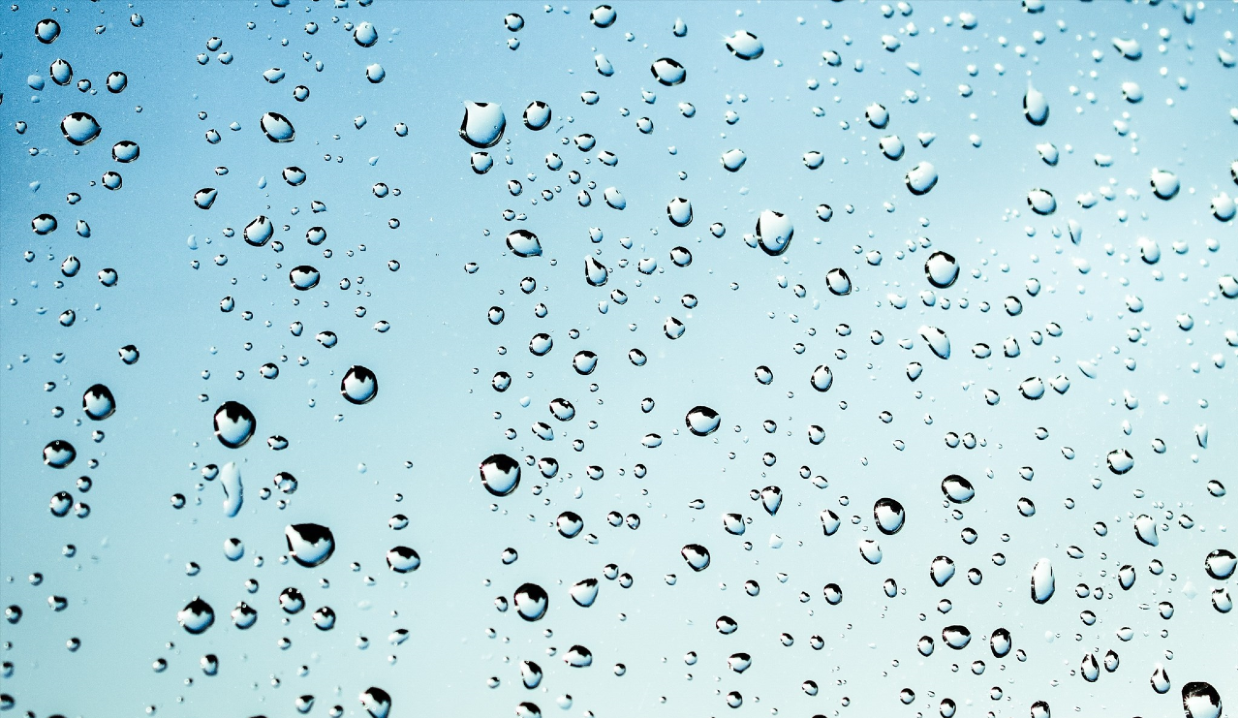
\includegraphics[width=\paperwidth]{Water3.png}};

\node[inner sep=0pt] (background) at (current page.center) {
\includegraphics[width=\paperwidth]{WaterBackground1R.png}};



\draw (current page.north west)node [fill=blue!5!white!10,fill opacity=.03,text opacity=1,inner sep=2cm]at (8,-16){ \Huge\centering\bfseries\sffamily\parbox[c][][t]{\paperwidth}{\centering \textcolor{Bittersweet}{Wastewater Treatment} \\\textcolor{BurntOrange}{Operations}\\[15pt] % Book title
% {\Large A Profound Subtitle}\\[20pt] % Subtitle
{}}}; % Author name
\end{tikzpicture}
%\begin{center}
%
\includegraphics[scale=0.5]{SCC_Logo_Primary.png}
%\end{center}
\vfill
\endgroup

%----------------------------------------------------------------------------------------
%	COPYRIGHT PAGE
%----------------------------------------------------------------------------------------

\newpage
~\vfill
\thispagestyle{empty}

\noindent Copyright \copyright\ 2021 Shabbir Basrai\\ % Copyright notice
%
%\noindent \textsc{Published by Publisher}\\ % Publisher
%
%\noindent \textsc{book-website.com}\\ % URL
%
%\noindent Licensed under the Creative Commons Attribution-NonCommercial 3.0 Unported License (the ``License''). You may not use this file except in compliance with the License. You may obtain a copy of the License at \url{http://creativecommons.org/licenses/by-nc/3.0}. Unless required by applicable law or agreed to in writing, software distributed under the License is distributed on an \textsc{``as is'' basis, without warranties or conditions of any kind}, either express or implied. See the License for the specific language governing permissions and limitations under the License.\\ % License information, replace this with your own license (if any)

\noindent \textit{Revision Date: November 8, 2021} % Printing/edition date

%----------------------------------------------------------------------------------------
%	TABLE OF CONTENTS
%----------------------------------------------------------------------------------------

%\usechapterimagefalse % If you don't want to include a chapter image, use this to toggle images off - it can be enabled later with \usechapterimagetrue

\chapterimage{WastewaterTreatmentPlantAerialBandW.jpg} % Table of contents heading image

\pagestyle{empty} % Disable headers and footers for the following pages

\tableofcontents % Print the table of contents itself

\cleardoublepage % Forces the first chapter to start on an odd page so it's on the right side of the book

\pagestyle{fancy} % Enable headers and footers again

\chapterimage{Water1.png} % Chapter heading image

\chapter{Why Treat Wastewater?}

\section{Definition of Wastewater}\index{Definition of Wastewater}


Wastewater is human-polluted water from home and industries. This includes water from:
\begin{itemize}
\item Flushing toilets and urinals  - blackwater.
\item Bathing, showering, and washing clothes and dishes  - greywater.
\item Commercial and industrial activities.
\item ...and often included is stormwater which contain pollutants washed off from inhabited areas - roads, parking lots, and rooftops.
\end{itemize}

\section{Why Treat Wastewater}\index{Why Treat Wastewater}
Although nature has an inherent capability to breakdown pollutants, given the large quantity generated from human activities, there is a need for centralized wastewater treatment plants to treat wastewater before releasing it back to the environment.  Wastewater from homes, businesses, and industries are collected in sewers for delivery to the treatment plant and subsequently discharged to a water body like a lake, river or ocean, or land, or reused. 

Wastewater treatment is designed to remove:
\begin{itemize}
\item organic matter
\item inorganic  pollutants including plant nutrients - nitrogen and phosphorous\\
\item pathogenic (disease causing) organisms\\
\end{itemize}

\section{Benefits of Treating Wastewater}\index{Benefits of Treating Wastewater}
Wastewater treatment protects:
\begin{itemize}
\item The environment
\item Human health
\end{itemize}

Specifically, wastewater treatment allows for the following:

\begin{enumerate}
\item \textbf{Mitigates deterioration of the receiving waters' ecosystem }\\
The discharge of inadequately treated wastewater will cause oxygen levels in the receiving waters to be depleted, due to:

\begin{itemize}

\item Wastewater containing nitrogen and phosphorus based pollutants (plant nutrients) entering a water body such as a lake or river will promote plant and algae growth which will seriously impact its normal aquatic life including fish through a process similar to the following:

\begin{itemize}
\item Nutrient promote algae bloom
\item Algae bloom prevent sunlight to the native plant spieces below the water's surface causing native plants to die
\item The organic material from the dead plants and algae promote growth of aerobic bacteria which will consume the dissolved oxygen in the water resulting in oxygen depletion.
\item The natural aquatic life including fish, frogs, and turtles will not be able to survive under oxygen depleted conditions and will die or leave that zone.
\end{itemize}
\item Other organic material present in wastewater will similarly promote growth of aerobic bacteria, intensifying the eutrophication of the receiving waters.
\end{itemize}

Thus, proper treatment of wastewater will prevent \hl{eutrophication} - which is the depletion of dissolved oxygen of the receiving water, consequently impacting/destroying its normal aquatic life.

\item \textbf{Removal of other harmful pollutants}\\
Organic and inorganic pollutants, including metals such as mercury, lead, cadmium, chromium and arsenic can have acute and chronic toxic effects on aquatic species and wildlife including migratory birds, are removed during the wastewater treatment process.
\item \textbf{Removal of pathogens}\\
Wastewater treatment removes parasites and disease-causing pathogens including bacteria and viruses for:
\begin{itemize}
\item People to continue enjoying recreational activities in the receiving bodies of waters such as lakes and rivers
\item Preventing the contamination of fish and other consumable products obtained from the waters
\item Allow the water body to remain as the source of potable water
\end{itemize}

\item \textbf{Reclaim water for recycle or reuse}\\
Besides protecting human health and the environment, wastewater treatment paves way for establishing the reuse or recycle of treated wastewater.  This benefit is particularly important for densely populated areas with limited access to fresh water supplies.  
\end{enumerate}

%
%can pollute beaches and contaminate shellfish populations, leading to restrictions on human recreation, drinking water consumption and shellfish consumption;
%Metals, such as mercury, lead, cadmium, chromium and arsenic can have acute and chronic toxic effects on species.
%Other substances such as some pharmaceutical and personal care products, primarily entering the environment in wastewater effluents, may also pose threats to human health, aquatic life and wildlife.
%\end{enumerate}
%In the receiving waters, inadequately treated wastewater discharge depletes dissolved oxygen levels - \hl{Eutrophication}, potentially .  Wastewater discharge promotes eutrophication due to:
%
%\begin{itemize}
%
%\item Nitrogen and phosphorus are essential for plant growth and are common ingredients in fertilizers. However, nutrient-rich wastewater entering a water body such as a lake or river will promote plant and algae growth which will seriously impact its normal aquatic life including fish through a process similar to the following:
%
%\begin{itemize}
%\item Nutrient promote algae bloom
%\item Algae bloom prevent sunlight to the native plant spieces below the water's surface causing native plants to die
%\item The organic material from the dead plants and algae promote growth of aerobic bacteria which will consume the dissolved oxygen in the water resulting in oxygen depletion - \hl{Eutrophication}.
%\item The natural aquatic life including fish, frogs, and turtles will not be able to survive under oxygen depleted conditions and will die or leave that zone.
%\end{itemize}
%
%
%\item Other organic material in present in wastewater, will similarly promote growth of aerobic bacteria intensifying the eutrophication of the receiving waters.  
%
%
%
%\end{itemize}
%
%
%%\end{enumerate)
%What is wastewater, and why treat it?
%Aerial view of a sewage treatment plant.
%The Central Wastewater Treatment Plant, Nashville, Tennessee.
%
%We consider wastewater treatment as a water use because it is so interconnected with the other uses of water. Much of the water used by homes, industries, and businesses must be treated before it is released back to the environment.
%
%If the term "wastewater treatment" is confusing to you, you might think of it as "sewage treatment." Nature has an amazing ability to cope with small amounts of water wastes and pollution, but it would be overwhelmed if we didn't treat the billions of gallons of wastewater and sewage produced every day before releasing it back to the environment. Treatment plants reduce pollutants in wastewater to a level nature can handle.
%
%Wastewater also includes storm runoff. Although some people assume that the rain that runs down the street during a storm is fairly clean, it isn't. Harmful substances that wash off roads, parking lots, and rooftops can harm our rivers and lakes.
%
% 
%
%Why Treat Wastewater?
%It's a matter of caring for our environment and for our own health. There are a lot of good reasons why keeping our water clean is an important priority:
%
%FISHERIES: Clean water is critical to plants and animals that live in water. This is important to the fishing industry, sport fishing enthusiasts, and future generations.
%
%WILDLIFE HABITATS: Our rivers and ocean waters teem with life that depends on shoreline, beaches and marshes. They are critical habitats for hundreds of species of fish and other aquatic life. Migratory water birds use the areas for resting and feeding.
%
%RECREATION AND QUALITY OF LIFE: Water is a great playground  for us all. The scenic and recreational values of our waters are reasons many people choose to live where they do. Visitors are drawn to water activities such as swimming, fishing, boating and picnicking.
%
%HEALTH CONCERNS: If it is not properly cleaned, water can carry disease. Since we live, work and play so close to water, harmful bacteria have to be removed to make water safe.
%
% 
%
%Effects of wastewater pollutants
%Stormsewer flowing both storm flow and sewage overflow during a major storm.
%Epic September 2009 flooding around Atlanta, Georgia. An overflowing sewer on Riverside Road, Roswell, Georgia. Likely this is a storm sewer, designed to carry stormwater runoff off of streets, that cannot handle the volume of runoff.
%In older sections of Atlanta there are combined sewer systems that are sewers that are designed to collect rainwater runoff, domestic sewage, and industrial wastewater in the same pipe. These overflows, called combined sewer overflows (CSOs) contain not only stormwater but also untreated human and industrial waste, toxic materials, and debris. They are a major water pollution concern for the approximately 772 cities in the U.S. that have combined sewer systems (EPA). The City of Atlanta is spending about \$3 billion dollars to put in separate storm and waste systems in the metro Atlanta area.
%
%Credit: Alan Cressler, USGS
%
%If wastewater is not properly treated, then the environment and human health can be negatively impacted. These impacts can include harm to fish and wildlife populations, oxygen depletion, beach closures and other restrictions on recreational water use, restrictions on fish and shellfish harvesting and contamination of drinking water. Environment Canada provides some examples of pollutants that can be found in wastewater and the potentially harmful effects these substances can have on ecosystems and human health:
%
%Decaying organic matter and debris can use up the dissolved oxygen in a lake so fish and other aquatic biota cannot survive;
%Excessive nutrients, such as phosphorus and nitrogen (including ammonia), can cause eutrophication, or over-fertilization of receiving waters, which can be toxic to aquatic organisms, promote excessive plant growth, reduce available oxygen, harm spawning grounds, alter habitat and lead to a decline in certain species;
%Chlorine compounds and inorganic chloramines can be toxic to aquatic invertebrates, algae and fish;
%Bacteria, viruses and disease-causing pathogens can pollute beaches and contaminate shellfish populations, leading to restrictions on human recreation, drinking water consumption and shellfish consumption;
%Metals, such as mercury, lead, cadmium, chromium and arsenic can have acute and chronic toxic effects on species.
%Other substances such as some pharmaceutical and personal care products, primarily entering the environment in wastewater effluents, may also pose threats to human health, aquatic life and wildlife.
% 
%
%Wastewater treatment
%The major aim of wastewater treatment is to remove as much of the suspended solids as possible before the remaining water, called effluent, is discharged back to the environment. As solid material decays, it uses up oxygen, which is needed by the plants and animals living in the water.
%
%"Primary treatment" removes about 60 percent of suspended solids from wastewater. This treatment also involves aerating (stirring up) the wastewater, to put oxygen back in. Secondary treatment removes more than 90 percent of suspended solids.
%
%
%In the simplest terms, wastewater is any amount of water that has been polluted by humans. This includes water contaminated as a result of:
%
%flushing toilets and urinals (this waste is known as blackwater)
%bathing, showering, and washing clothes and dishes (greywater)
%commercial and industrial activities
% 
%As you would expect, wastewater is almost entirely water. The remaining portion — roughly 0.1% — contains organic matter, inorganic compounds, nutrients, and microorganisms that need to be explored in more detail.
% 
%
%Organic matter
%Salmo trutta, commonly known as brown trout, spawning in a shallow river.
%Organic matter in wastewater includes proteins, carbohydrates, fats, oils, greases, and synthetic compounds found in certain detergents.
%
%Without proper treatment, organic matter enters lakes and rivers and becomes a food source for the microorganisms that live there. The problem is that these tiny creatures pull dissolved oxygen from water when they break down pollutants. The more pollutants there are in the water, the greater their demand for oxygen.
%
%This process spins out of control in lakes and rivers with large amounts of organic matter. In these watercourses, oxygen levels fall so low that animals like fish, frogs, and turtles suffocate and die.
% 
%
%Inorganic compounds
%Wastewater sampling and testing equipment in a laboratory.
%Inorganics in wastewater include compounds with copper, lead, magnesium, nickel, potassium, sodium, or zinc. In many cases, these harmful substances are the byproducts of commercial and industrial activities.
%
%Inorganics do not break down easily. If they enter lakes or rivers via untreated wastewater, they remain there. As their concentrations increase over time, the water quality becomes a hazard for humans and animals alike.
% 
%
%Nutrients
%A cyanobacteria blue-green algae bloom in a river.
%Nutrients in wastewater include nitrogen and phosphorus compounds. These often come from human waste and cleaning products like laundry detergent and dishwasher soap.
%
%It is no secret that nitrogen and phosphorus are common ingredients in fertilizers. They work wonders when we want to make plants grow and reproduce. But this advantage becomes a serious threat if we allow untreated and nutrient-rich wastewater to enter lakes and rivers.
%
%High concentrations of nitrogen or phosphorus can lead to "dead zones" in watercourses. The process goes like this:
%
%Excess nutrients feed the growth of large algae blooms.
%Algae blooms prevent sunlight from reaching plants below the water's surface.
%Native plant species die without sunlight.
%Bacteria that feed on decaying plant matter multiply.
%Growing populations of bacteria consume more and more dissolved oxygen in the water.
%Fish and other aquatic species that need oxygen leave the watercourse or die.
% 
%Nitrogen in untreated wastewater can cause another problem. If nitrate (a nitrogen compound) pollutes our drinking water, it can reduce our blood's ability to transport oxygen. For infants, this can lead to what is commonly known as blue baby syndrome. In extreme cases, the condition is fatal.
% 
%
%Microorganisms
%Microscopic view of E. coli bacteria in a wastewater sample.
%Some microorganisms in wastewater are helpful because they break down organic matter that would otherwise pollute the environment.
%
%Pathogens in untreated wastewater are a different story. These bacteria, parasites, and viruses can contaminate clean water sources. If they do, they undermine human health by causing serious and sometimes deadly illnesses.
%
%Perhaps the best-known example took place in Walkerton, Ontario, Canada. In May 2000, the town's drinking water supply was tainted with E. coli bacteria because municipal wastewater was not properly treated. More than 2,300 residents became ill and seven people died.
% 
%
%Why is wastewater treatment important?
%A closer look at wastewater makes it easy to see why effective treatment is so important.
%
%Think of your on-site wastewater treatment plant as a water conservation tool. By removing suspended solids and other pollutants, your system prevents groundwater and water pollution that could lead to:
%
%tainted drinking water
%water scarcity and water shortages
%foul lakes and rivers
%lower numbers of aquatic species
%dangers to livestock
%reduced waterfront property values
% 
%Now that you understand the basics of wastewater, take your knowledge to next level. Discover our range of treatment systems and find out how they protect your property, our communities, and planet we share.


% \pagebreak
% \begin{center}
% \phantom{A}
% \vspace{10cm}

% BLANK PAGE
% \end{center}
% \pagebreak
\chapterimage{RegulationsChapterImage.png} % Chapter heading image
\chapter{Regulations}
\section{Regulations Related to Wastewater Treatment}\index{Regulations Related to Wastewater Treatment}
The main objective of these regulations is to ensure appropriate quality of the treated wastewater.  

\subsection{Treated Wastewater - NPDES Permit}\index{Treated Wastewater - NPDES Permit}
The National Pollutant Discharge Elimination System (NPDES) permit program program addresses water pollution by regulating point sources that discharge pollutants to waters of the United States.

\begin{itemize}
\item The NPDES permit program was created in 1972 by the Clean Water Act (CWA)and is administered by the federal USEPA.
\item Applies to sources that discharge pollutants to waters of the United States.
\item Requires all facilities discharging “pollutants” into any body of water in the USA to obtain and comply with a \hl{NPDES permit}.
\item NPDES permit \hl{establishes} \textul{discharge limits}, \textul{monitoring} and \textul{reporting} \hl{requirements}\\
\item In California, the responsibility of implementing the federal NPDES program is delegated to the State of California through the State Water Resources Control Board (State Water Board or SWRCB) and finally to the nine Regional Water Quality Control Boards (Regional Water Boards or RWQCB), collectively known as Water Boards. 
\item The RWQCB issues the NPDES permit.
\end{itemize}

\subsection{Influent Wastewater - National Pretreatment Program}\index{Influent Wastewater - National Pretreatment Program}
Municipal wastewater treatment plants also known as Publicly Owned Treatment Works (POTWs) implement and enforce their Pretreatment or Industrial Discharge Control programs to meet Federal and State regulations requirements related to wastewater discharges from industrial sources.  The national pretreatment program is a component of the NPDES program and is also known as the Source Control Program\\

The Pretreatment/Source Control program is for controlling industrial (non-domestic) wastewater discharges with the following objectives:
\begin{enumerate}
\item Protect the treatment plant operations so that the industrial discharge does not contain pollutants or have certain characteristics (including pH, temperature) which could adversely effect the treatment process or impact public safety and the safety of the people working at the treatment plant.
\item Prevent the introduction of pollutants that could pass through untreated and into the receiving body of water.

\item Improve opportunities for reuse or recycling of wastewater and sewage sludge.

\end{enumerate}

In California:
\begin{enumerate}
\item Wastewater treatment plants are required to have a Pretreatment Program when their total design flows are greater than five million gallons per day (5 mgd). 
\item Facilities with smaller flows (5 mgd or less) may also be required to implement a Pretreatment Program if they receive industrial waste and pretreatment is warranted.
\item The Pretreatment Program for a wastewater treatment entity is reviewed and approved by the State and Regional Water Boards, and 
\item The Pretreatment Program's monitoring and reporting requirements are incorporated in the facility's NPDES permit.
\end{enumerate}

\section{Sewage Sludge/Biosolids Regulations}\index{Sewage Sludge/Biosolids Regulations}
Sewage sludge or biosolids is a byproduct of wastewater treatment.  The biosolids produced are disposed or used using methods including land application, landfill and incineration.  Federal Regulation 40CFR Part 503 also known as Rule 503 establishes the standards for the use or disposal of wastewater biosolids - as stipulated under the Clean Water Act.  The facility's NPDES permit incorporates the applicable federal, state and local requirements as they apply to its biosolids.
			\begin{itemize}
				\item Part 503 rule applies to any person who applies biosolids to the land or fires biosolids in a biosolids incinerator, and to the owner/operator of a surface disposal site, or to any person who is a preparer or generator of biosolids for use, incineration, or disposal.
				\item Part 503 standard includes:
					\begin{enumerate}
						\item General requirements which establishes the purpose and applicability of the rule, the compliance period, and exclusions from the rule.
						\item Limits on heavy metals content
						\item Solids management practices related to use and disposal of wastewater biosolids
						\item Operational standards related to biosolids management, and
						\item Requirements for the frequency of monitoring, record-keeping, and reporting
					\end{enumerate}
			\end{itemize}
Part 503 requirements are factored in when establishing the heavy metals concentration limits for the Pretreatment or Industrial Control Program as a significant portion of the heavy metals in the influent wastewater are removed as part of the wastewater solids.

\section{Air Quality Regulations}\index{Air Quality Regulations}
\begin{itemize}
\item Air emissions from wastewater collections and treatment systems are subject to federal, state and local air quality related rules and regulations established to protect human health and comfort, and the environment.  
\item Typically, a local agency such as the South Coast Air Quality Management District (SCAQMD) is designated to enact and enforce air quality rules and regulations, through its permitting process, applicable to all sources of air emissions including wastewater treatment plants.\\

\item Systems/processes subject to air quality regulations at air quality regulations include:

\begin{itemize}
\item Fugitive emissions:  Foul air containing compounds such as hydrogen sulfide and organics, which escape from process tanks, pipes and associated structures such as manholes and wetwells, is potentially harmful for the affected public and also cause odors.  
\item Digester gas combustion:  Digester gas a product of wastewater solids treatment contains methane and is either combusted in power generation equipment or burned in flares.
\item Odor control systems:  These commonly used systems are for controlling emissions of regulated pollutants such as ammonia and to prevent odors associated with compounds such as hydrogen sulfide.
\end{itemize}
 
\item Related to its air pollutants emissions, wastewater treatment plants are required to:
\begin{itemize}
\item Obtain air quality related operating permits for equipment and processes which emit air pollutants and for its systems treating foul air.
\item Implement air emission pollutants control measures
\item Comply with record keeping and reporting requirements
\item Comply with air quality rules to prevent public nuisance and protect public health and safety
\end{itemize}

\end{itemize}

\section{Regulations Related to Operations and Maintenance}\index{Regulations Related to Wastewater Treatment Operations and Maintenance}
\subsection{Operator Certification}\index{Operator Certification}
\begin{itemize}
\item The requirements of the Operator Certification program is established for each state.  These meet the Operator Certification Requirements of the regulations stemming from the 1996 Amendments to the Safe Drinking Water Act.
\item The goal is to ensure that operators of wastewater treatment facilities in the State meet the minimum level of competence; thereby, protecting public health and the environment.
\item In California, the Wastewater Operator Certification program (WWOCP) administers Wastewater Treatment Plant Certification examinations, certifications (grades I to V), and certification renewals. 
\item WWOCP classifies Wastewater Treatment Plants and stipulates that no person shall operate a wastewater treatment plant unless that person has been certified by the division as a wastewater treatment plant operator or operator-in-training at a grade appropriate for the class of plant being operated.
\item A certified operator or operator-in-training may be subject to administrative sanctions including reprimand or denial, suspension, probation, or revocation of the operator certification for performing, or allowing or causing another to perform acts which include:
\begin{itemize}
\item Operating or allowing the operation of a wastewater treatment plant by a person who is not certified at the grade necessary for the position
\item failing to use care or good judgment in the course of employment as an operator or failing to apply knowledge or ability in the performance of duties.
\item Negligence causing the violation of appropriate waste discharge requirements of the NPDES permit
\end{itemize}
\end{itemize}
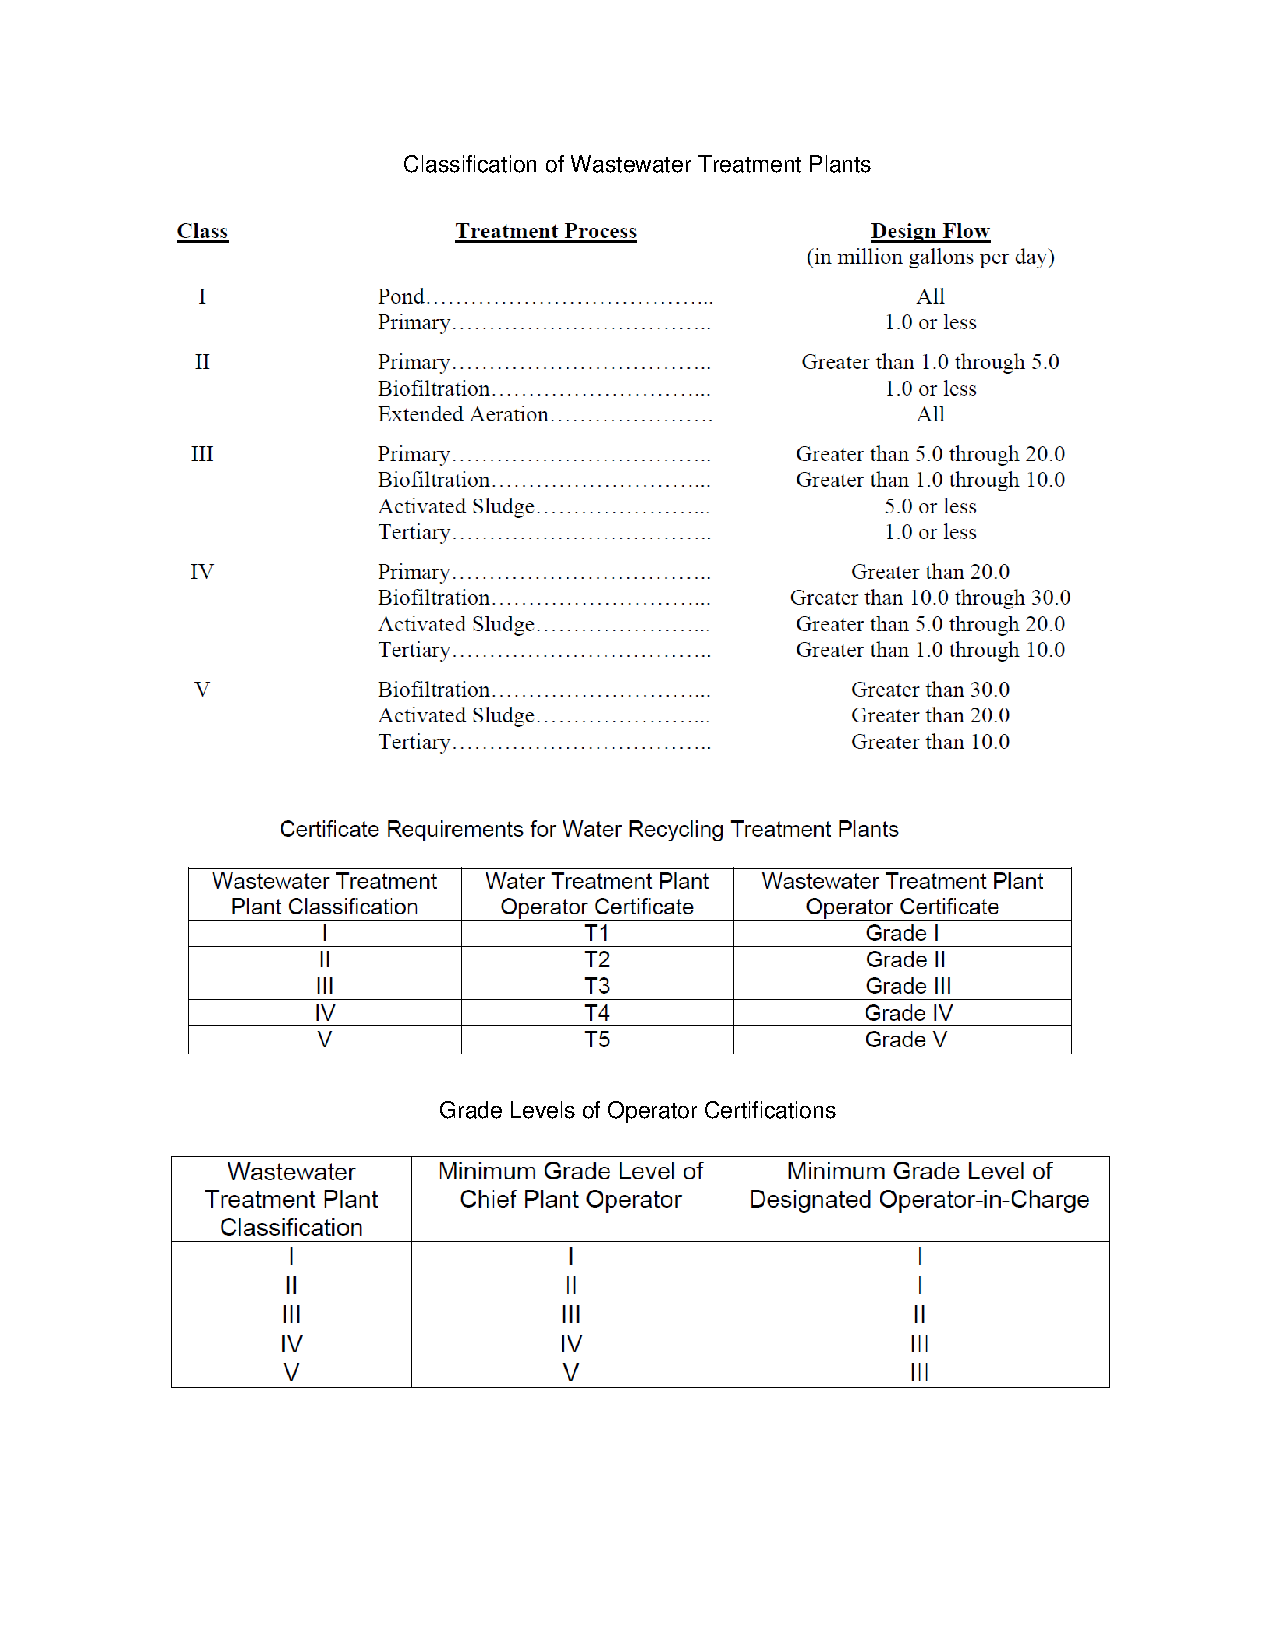
\includepdf[pages=-]{WastewaterPlantOperatorClassificationRequirements.pdf}
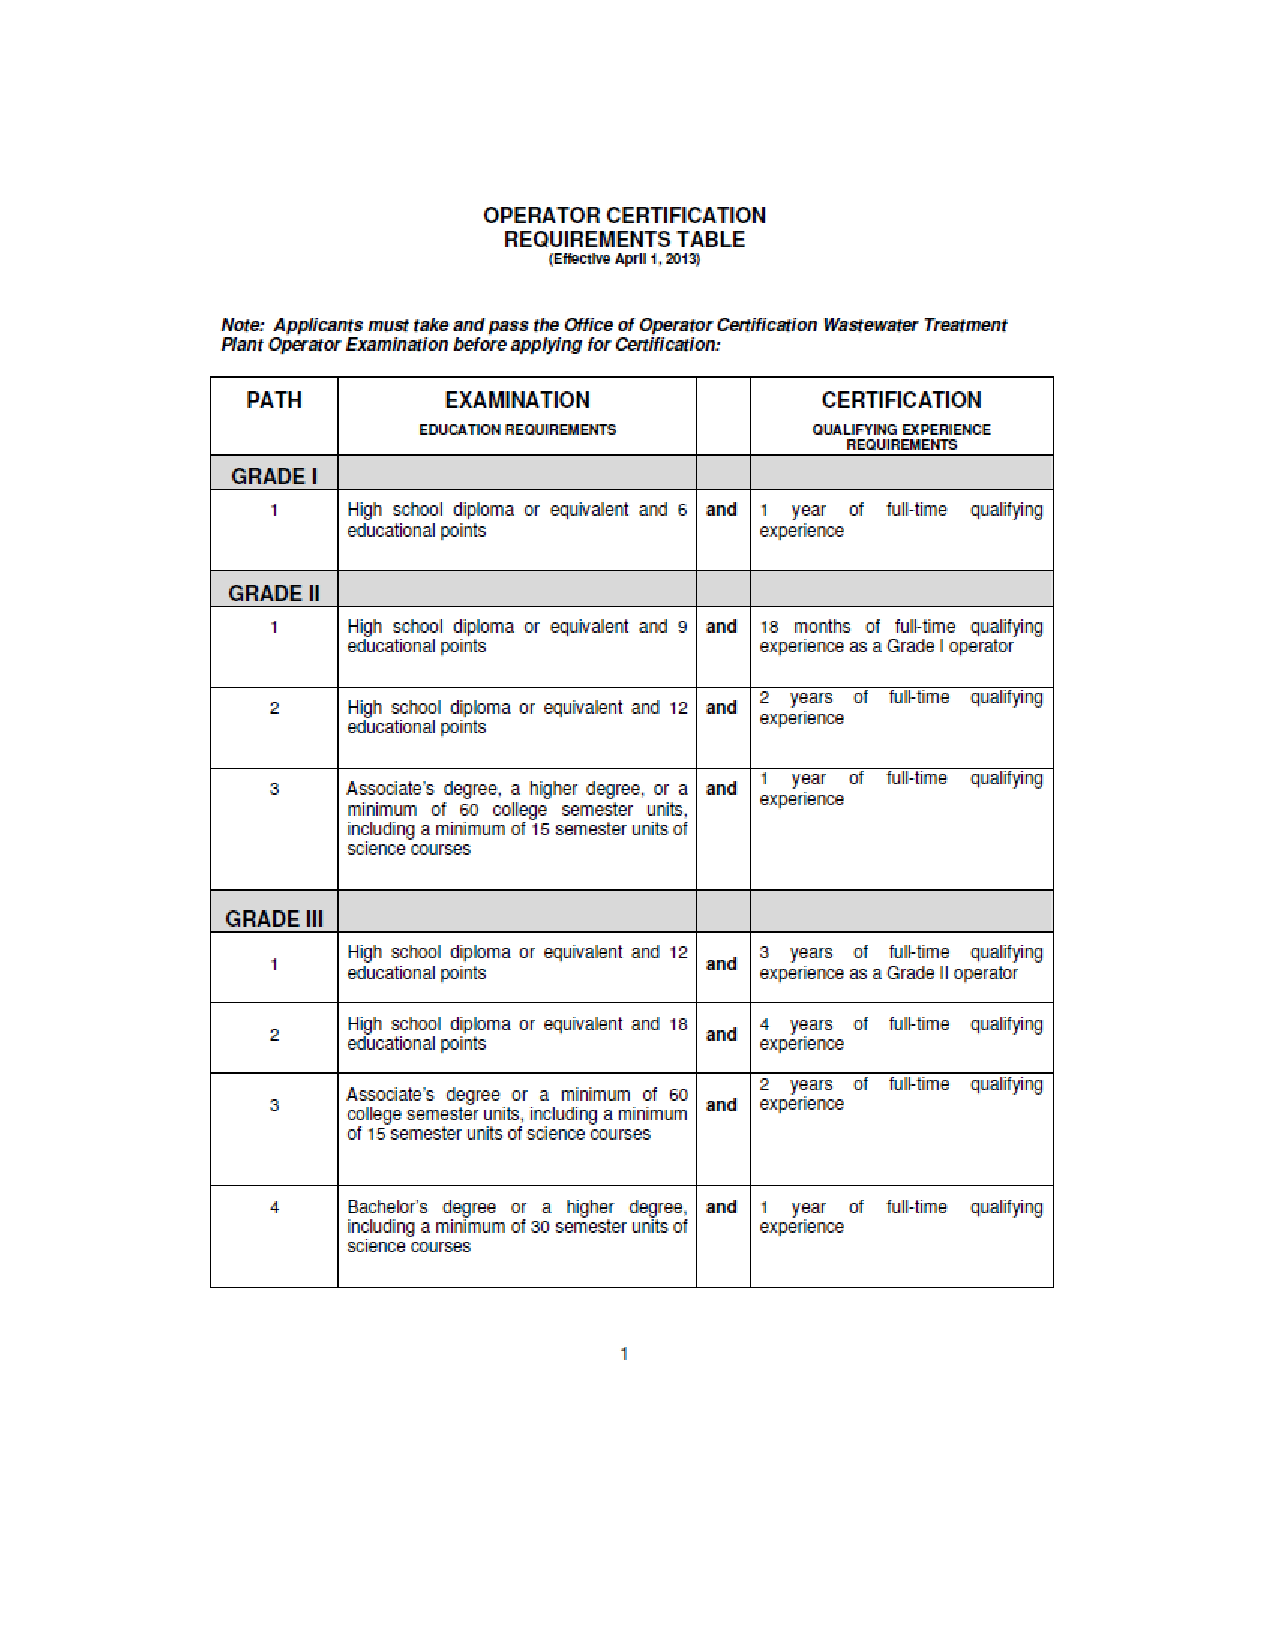
\includepdf[pages=-]{CertificationRequirement.pdf}

\subsection{Worker Safety}\index{Worker Safety}
\begin{itemize}
\item Wastewater treatment facility can be an extremely unsafe occupational field
\item It involves most of the major categories of workplace hazards:  biological, chemical, physical, safety and ergonomic,  accentuated with other factors such as shift work and diverse tasks.
\item Entities including The Occupational Safety and Health Administration(OSHA) National Electrical Code (NEC), National Fire Protection Association (NFPA), Underwriters Laboratory (UL) have recognized these hazards and implemented codes and standards to protect the affected persons and wastewater workers.
\end{itemize}

\chapterimage{Laboratory}

\chapter{Constituents Properties and Analysis}\index{Constituents Properties and Analysis}


\section{Wastewater Constituents} \index{Wastewater Constituents}
		\subsection{Organics}\index{Organics}		
		\begin{itemize}
			\item The main reason for treating domestic wastewater is to remove the organic matter.  
			\item Organics are substances containing carbon, hydrogen and oxygen, and some of which may be combined with nitrogen, sulfur or phosphorous.
			\item About 50 percent of the solids present in wastewater are organic.  This fraction is generally of animal or vegetable life, dead animal matter, plant tissue or organisms, and also include synthetic organic compounds.
			\item The principal organic compounds present in domestic wastewater are proteins, carbohydrates and fats together with the products of their decomposition.
			\item Organics are subject to decay or decomposition through the activity of bacteria and other living organisms.  \hl{Since the organic fraction can be driven off at high temperatures, they are also called \textbf{volatile solids}}.\
			\item \emph{Organics in wastewater is typically quantified in terms of oxygen required to oxidize the carbon based material present} in wastewater using the following methods:\\
\subsubsection{Biochemical Oxygen Demand (BOD)}\index{Biochemical Oxygen Demand (BOD)}

			  %     \begin{enumerate}[i.]
			  %     	\definecolor{shadecolor}{RGB}{220,220,220}
					% %%%%%%%%%%%
					% % LEVEL 4 %
					% %%%%%%%%%%%
			  %     	\begin{snugshade*}
			  %     		\item \noindent\textsc{Biochemical Oxygen Demand (BOD)}%@@@@@@@@@@@@@@@@@@%
			  %     	\end{snugshade*}					
			      	\begin{itemize}
			      		\item Oxygen is required for the consumption of organic matter by aerobic bacteria
			      		\item BOD test measures the depletion of oxygen in a wastewater sample over a five day period
			      		\item BOD measures the organic content in terms of oxygen required for the microorganisms to consume the organic material present

			      		\item BOD is typically measured as BOD$_5$ which is the oxygen demand of the wastewater measured after 5 days of the initiation of the test.
			      		\item The test involves incubating a known dilution of wastewater in a 300 ml bottle for 5 days at 20\si{\degree}C.  The dissolved oxygen (DO) content at the start and end of the incubation period is used for calculating the BOD.
			      		\item For the test to be considered valid, the following criteria need to be met: 1) DO consumption during the test must be at least 2 mg/l, 2) DO remaining at the end of the test must be at least 1 mg/l, and 3) DO consumed in blank should be 0.2 mg/l or less
			      		      			
			      		\item BOD is a parameter to measure the strength of wastewater and the measurement of the wastewater treatment plant or treatment process influent and effluent BOD is standard practice to measure its performance.  Typical domestic wastewater BOD is about 200-250 mg/l.
			      		\item The oxygen consumed by the microorganisms during the BOD test is primarily for: 1) Oxidizing the carbonaceous material (cBOD – carbonaceous BOD), and 2) Oxidizing nitrogenous constituents such as ammonia (nBOD – nitrogenous BOD).
			      		\item Thus, BOD (Total) = cBOD + nBOD.  The cBOD and nBOD is measured by adding certain chemical inhibitors which will inhibit the bacteria responsible for consuming the nitrogenous matter, thus measuring only the cBOD as part of the BOD test.
			      		\item Since not all of the organics is metabolized in the 5 days of the regular BOD test, certain wastewater discharge permits require reporting of the ultimate BOD value (BOD$_U$)\\
			      	\end{itemize}

			    \subsubsection{Chemical Oxygen Demand (COD)}\index{Chemical Oxygen Demand (COD)}
			      	% \begin{snugshade*}
			      	% 	\item \noindent\textsc{Chemical Oxygen Demand (COD)}%@@@@@@@@@@@@@@@@@@%
			      	% \end{snugshade*}		  
			      	\begin{itemize}
			      		\item The COD test involves using chemical oxidizers to measure the oxygen demand of the wastewater.
			      		\item As the chemical oxidizers will oxidize other constituents present, including inorganic matter, the COD value of wastewater will be higher than the BOD.  
			      		\item The COD test can be conducted rather quickly than the 5 day BOD test, it is an effective method to quantify the wastewater strength and process efficiencies and allow operators to make timely process adjustments.
			      	\end{itemize}

			    \subsubsection{Total Organic Carbon (TOC)}
			      	% \begin{snugshade*}
			      	% 	\item \noindent\textsc{Total Organic Carbon (TOC):}\\%@@@@@@@@@@@@@@@@@@%
			      	% \end{snugshade*}
			      	The TOC method utilizes laboratory analytical instruments which directly measure the organic carbon content by quantifying the amount of carbon dioxide produced from the complete combustion of the organics present.
			      % \end{enumerate}
		\end{itemize}
		
		
		
			\hl{Note: BOD measures the amount of oxygen required by the microorganisms present to consume the organic material while COD measures the chemical oxidation required to oxidize all chemicals including organics present in wastewater.  BOD value of typical domestic sewage is about 200 - 250 mg/l while the COD value ranges from 300 - 450 mg/l.  Typical BOD:COD ratio ranges from 0.5-0.8.}\\


\subsection{Solids}\index{Solids}
% 		\pagebreak
% 				\begin{snugshade*}
% 			\item \noindent\textsc{Solids}
% 		\end{snugshade*}	
		Like BOD, wastewater solids is another critical parameter for establishing the wastewater strength and determining treatment process efficiencies. 
		\begin{itemize}
			\item The \texthl{solids can be classified as suspended or dissolved} based upon its ability to pass through a standardized filter paper.
			\item When the wastewater is filtered:
			      \begin{itemize}
			      	\item the residual solids remaining on the filter paper after drying in an oven at 103\si{\degree}C is the \hl{suspended solids} portion, and 
			      	\item the solids remaining after drying the filtrate are the \hl{dissolved solids}.
			      \end{itemize}
			\item Suspended solids include larger floating particles and consist of sand, grit, clay, fecal matter, paper, pieces of wood, particles of food and garbage, and similar materials.
			\item Suspended solids can be categorized based upon its settling characteristics as:
			      \begin{itemize}
			      	\item \hl{Settleable}
			      	\item \hl{Non-settleable}
			      	      \begin{itemize}
			      	      	\item \hl{Colloidial}-small, charged (typically negative) particles which do not settle easily.  Some of the colloidial particles are small enough to pass through the filter paper used for filtering the suspended solids
			      	      	\item \hl{Floatable}-example oil and grease and small plastics
			      	      \end{itemize}
			      \end{itemize}
			\item Dissolved solids in wastewater include organics.  However, the major elements of dissolved solids are inorganic ions such as Ca$^{+2}$, Mg$^{+2}$, Cl$^-$, SO$_4$ $^{-2}$ , HCO$_3$ $^-$, Fe$^{+2}$, PO$_4$ $^{-3}$, NO$_3$ $^-$.  These ions are part of the dissolved salts such as sodium chloride (NaCl), calcium bicarbonate (Ca(HCO$_3$)$_2$), magnesium phosphate (Mg$_3$PO$_4$) and others which are normally present in water and wastewater. 
			      \begin{itemize}
			      	\item Conductivity or electrical conductance (EC) measurement is typically conducted as the wastewater enters the plant as \hl{conductivity provides an indirect and simple measure of the amount of dissolved solids present.}  
			      	\item Conductivity or electrical conductance (EC) is a measure the amount of electrical current that can be conducted by a solution.  
			      	\item The conductance of electricity in a solution is due to the presence of dissolved inorganic ions 
			      	\item The higher the concentration of these ions, the higher is the conductivity. 
			      	\item \underline{Conductivity is measured in the units of mhos/cm or Siemens/cm.}  (Note:  mhos is the reverse of ohm which is a measure of resistance).
			      	\item Typical wastewater conductivities range from 50 to 1500 S/cm
			      \end{itemize}
			\item Both suspended and dissolved solids can be either \hl{volatile (organic)} or \hl{fixed (inorganic)}.
			\item \hl{Total Solids is thus a sum of TSS and dissolved solids or volatile and fixed solids.}
			      \begin{itemize}
			      	\item The volatile solids are typically of plant or animal origin .
			      	\item The fixed solids include sand, gravel and silt as well as the dissolved salts.
			      \end{itemize}
			      \begin{minipage}{0.5\textwidth}
			      	\item The volatile or fixed fractions are quantified by incinerating the solids in a muffler furnace at 550\si{\degree} which removes only the volatile solids leaving only the fixed solids behind.
			      	\item In terms of the size of the solids, the distribution is approximately thirty percent suspended and about seventy percent dissolved solids - which includes the colloidal particles which have passed through the filter paper.\\ 
			      	\item As primary treatment process involve settling of solids, establishing the settleable portion of the suspended solids is important.\\  
			      	\item \hl{The settleable solids are quantified using an Imhoff cone and are reported in ml/L}.  Imhoff cone is a 1 liter, clear cone shaped container, with volume graduations (ml) at the bottom.
			      						
			      \end{minipage}	
			      \begin{minipage}{0.5\textwidth}
			      	\begin{center}
			      		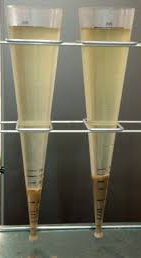
\includegraphics[scale=0.7]{ImhoffCone}\\
			      		Imhoff Cone\\
			      		\textit{Note the ml markings at the bottom of the cone}
			      		
			      		
			      	\end{center}
		      \end{minipage}
%			      \end{minipage}
			      	\item One factor which affects settleability is the conveyance time of the sewage to the treatment plant. 			
			      	\item The settleable component of the suspended solids will decrease as the sewage becomes more septic due to longer conveyance times.
			\item Influent and effluent total suspended solids are measured to establish the overall treatment and individual process efficiencies.  
			\item Volatile solids measurements before and after biological processes such as secondary treatment and digestion provide information on the process efficiency.\\
		\end{itemize}

% 			\end{enumerate}
	\subsubsection{Summary of Wastewater Solids}\index{Summary of Wastewater Solids}		
% 			\begin{snugshade*}
% 				\item \noindent\textsc{Summary of Wastewater Solids}
% 			\end{snugshade*}
			\begin{itemize}
				\item Solids in wastewater can be categorized as dissolved or suspended
				      \begin{itemize}
				      	\item Suspended solids can be further categorized as settleable or unsettleable
				      \end{itemize}
				\item Solids can also be categorized as organic (aka: volatile) or inorganic (aka: fixed)
				\item Colloidial particles are small sized particles some of which pass through the filter and accounted as part of dissolved solids
				\item TSS - Total Suspended Solids are the solids that are captured on the filter paper upon filtration of the wastewater sample.  
				\item Wastewater samples typically analyzed for TSS include:  plant, primary and secondary processes - influent and effluent.  TSS is reported in mg/l
				\item TS - Total Solids are solids content of sludge.  TS of sludge is established by drying a preweighed quantity of sludge in an oven and is typically reported as \% solids - which is how many parts (by weight) of solids per 100 parts (by weight) of sludge.
				\item Volatile solids are solids that are removed when the solids are incinerated at 550C.  The solids that remain after incineration are fixed or non-volatile or inorganic solids.
			\end{itemize}
	\subsubsection{Wastewater Solids Content}\index{Wastewater Solids Content}			
% 			\begin{snugshade*}
% 				\item \noindent\textsc{Typical influent wastewater contains:}
% 			\end{snugshade*}
			\begin{itemize}
				\item Less than 0.1\% total solids.  Total solids concentration in typical wastewater is about 750mg/l
				\item The total solids are 50\% organic (volatile) and 50\% inorganic (fixed)
				\item Of the total solids, dissolved solids constitute about 70\% of the solids and the remaining 30\% solids are suspended solids
				\item 40\% of the dissolved solids are volatile the remaining 60\% are fixed
				\item 70\% of the suspended solids are volatile and the remaining 30\% are fixed
			\end{itemize}
			% \clearpage\thispagestyle{empty}
			\begin{figure}[!htbp]
			\vspace{2cm}
				\begin{center}
					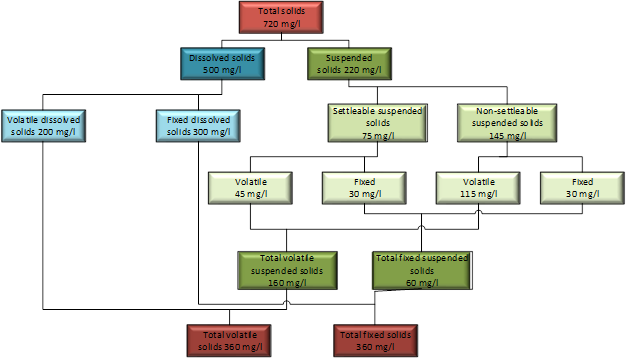
\includegraphics[scale=0.8]{WastewaterSolids}\\
					\caption{Typical Wastewater Solids Concentrations}
				\end{center}
				\end{figure}
% % 			\end{enumerate}
				
\subsection{Nutrients}\index{Nutrients}	
% 			\begin{snugshade*}
% 				\item \noindent\textsc{Nutrients}
% 			\end{snugshade*}	
			\begin{itemize}
				\item Plant nutrients - nitrogen and phosphorous, present in wastewater effluent discharge, promote growth of plant and algal matter in the receiving waters causing destruction of the normal aquatic life mainly due to oxygen depletion - eutrophication.
				      
				\item Because of the potential impacts of the presence of these nutrients in wastewater effluent on the receiving waters,  limits on the levels of these nutrients is typically stipulated in the treatment plant's wastewater discharge permit.
				      
				\item Typically, conventional secondary treatment processes are designed primarily remove the organics from the wastewater.  Secondary treatment process designed to additionally remove nutrients is deemed as tertiary or advanced treatment is termed as Biological Nutrient Removal (BNR).
			\end{itemize}
	\subsubsection{Nitrogen}\index{Nitrogen}				
% 			\begin{enumerate}%@@@@@@@@@@@@@@@@@@%
% 				\definecolor{shadecolor}{RGB}{220,220,220}
% 				\begin{snugshade*}
% 					\item \noindent\textsc{Nitrogen}%@@@@@@@@@@@@@@@@@@%
% 				\end{snugshade*}

	\textbf{Forms of nitrogen:}\\	
% 				\begin{itemize}
% 					\item Forms of nitrogen:\\
					      \begin{itemize}
					      	\item About 60\% of nitrogen in wastewater is present as ammonia nitrogen (about 60\%).  The ammonium nitrogen is present either in the form of ammonia (NH$_3$ ) or as ammonium (NH$_4^+$ ) ion.   These two forms can rapidly change from one to the other depending on pH and temperature.  Under low pH (acidic) or neutral conditions – pH less than or equal to 7, ammonia exists mostly as ammonium.  Ammonia becomes the dominant form as the pH increases to 8 and beyond.
					      	\item The other dominant form of nitrogen, about 40\% of the total nitrogen is as organic nitrogen
					      	\item Nitrogen measured as Total Kjeldahl Nitrogen (TKN) which is the sum of the organic nitrogen and the ammonia nitrogen concentrations.  Total inorganic nitrogen is the total concentration of ammonia nitrogen, NO3-, and NO2-.   Table provides the concentrations and forms of nitrogen in wastewater.
					      \end{itemize}
					      \setlength{\arrayrulewidth}{0.7mm}
					      \setlength{\tabcolsep}{8 pt}
					      \renewcommand{\arraystretch}{0.8}
					      \begin{center}
					      \begin{figure}[!htbp]
					      	\noindent \begin{tabular}[!htbp]{ |p{6cm}|p{2.0cm}|p{2.5cm}|p{2.cm}|}
					      	\hline
					      	\multicolumn{4}{|c|}{\textbf{Forms of Nitrogen in Wastewater}} \\
					      	\hline
					      	%\thead{A Head} & \thead{A Second \\ Head} & \thead{A Third \\ Head} \\
					      	%\hline%
					      	
					      	\hspace{1.8 cm}Forms of Nitrogen & \hspace{0.25 cm} Formula & \hspace{.4 cm} Found in & \hspace{.4 cm} Typical \newline \hspace{.2 cm}Concentration\\
					      	\hline
					      	\small Ammonia/Ammonium & \small NH$_3$/NH$_4^{\enspace +}$ &  \small Influent wastewater & 30-50 mg/l\\
					      	
					      	Total Kjeldahl Nitrogen \newline  \small (Ammonia/Ammonium + Organic Nitrogen) &  \small TKN &  \small Wastewater \newline  \small effluent  & 30-60 mg/l \\
					      	
					      	\small Total Inorganic Nitrogen \newline  \small (Ammonia/Ammonium + Nitrite + Nitrate) & \small TIN &  \small  Wastewater \newline  \small effluent  & 1-40 mg/l \\
					      	
					      	\small Nitrate  & $NO_3^{\enspace -}$ &  \small Nitrified effluent &  \small 1-35 mg/l \\
					      	
					      	\small Nitrate  &  $NO_2^{\enspace -}$ &  \small Partially nitrified effluent &  \small 0.1-2 mg/l \\
					      	
					      	\hline
					      	\end{tabular}
					      	\caption{Forms of Nitrogen}
					      	\end{figure}
					      \end{center}
					      
		\subsubsection{Phosphorous}\index{Phosphorous}			
		\textbf{Forms of phosphorous:}\\
					      \begin{itemize}
					      	\item The principal forms are organically bound phosphorus, polyphosphates, and orthophosphates.
					      	\item Organically bound phosphorus originates from body and food waste and, upon biological decomposition of these solids, is converted to orthophosphates. 
					      	\item Polyphosphates originate from synthetic detergents and are hydrolyzed to orthophosphates. Thus, the principal form of phosphorus in wastewater is assumed to be orthophosphates, although the other forms may exist. Orthophosphates consist of the negative ions PO$_4$$^{3-}$, HPO$_4$$^{2-}$, and H$_2$PO$_4$ $^-$.  These may form chemical combinations with cations (positively charged ions).
					      \end{itemize}

\subsubsection{Oil and Grease}\index{Oil and Grease}	
			Fats, oil and grease in wastewater originate from homes, food establishments and industries.
			\begin{itemize}
				\item Oil and grease content of wastewater is established in the laboratory by extracting it with a solvent - \textit{n}-hexane.  The concentration of oil and grease is reported in mg/l and typical oil and grease content of wastewater ranges from 80 - 120 mg/l
				\item Presence of excessive oils and grease could potentially impact the secondary treatment process
				\item Oils and grease are removed as floatables in primary treatment and sent with the sludge to the digesters
			\end{itemize}

\section{Wastewater Properties and Parameters} \index{Wastewater Properties and Parameters}
			
		Laboratory and field tests are conducted to measure parameters which are critical for monitoring and controlling treatment.  The following are the key parameters that are measured.	
			
\subsection{pH}\index{pH}	
			\hl{pH is a measure of the hydrogen ion (H$^+$) content or the acidity or basicity of a solution.}  pH impacts the chemical and micribiological elements of wastewater treatment processes and thus pH measurement and control is critical.
			\begin{itemize}
				\item Pure water dissociates into equal concentration of hydrogen ions and hydroxide ions:\\ 
				      $H_2O \rightarrow H^+ + OH^-$.
				\item The H$^+$ are responsible for acidic properties and the OH$^-$ ions for the basic properties.  
				\item pH is the inverse of H$^+$ concentration; pH increases when the concentration of H$^+$ decreases relative to the concentration of OH-. 
				\item pH scale ranges from 0 – 14. When the concentration of both H$^+$ and OH$^-$ are equal, as in pure water, it is considered neutral and its pH is 7.0.  \item If the pH of a sample solution is below 7.0, the sample is termed acidic and is alkaline or basic if its pH is above 7.0. 
				\item Each change of 1 pH unit represents a 10 fold change in concentration.  For example, a sample with a pH of 2.0 is 1000 times more acidic than a sample with a pH of 5.0. 
				\item pH is measured by an electrode that is sensitive only to H$^+$ or using a pH strip which is essentially an adsorbent paper which is pre-impregnated with chemicals which change color under different H$^+$ concentrations.
				\item Most organisms involved in biological wastewater treatment processes do well within a a narrow range of pH near neutral (pH of 7).			
			\end{itemize}
			
\subsection{Oxidation Reduction Potential (ORP)}\index{Oxidation Reduction Potential (ORP)}			
			\begin{itemize}
				\item ORP measurements are common in wastewater process control for monitoring conditions and process efficiency
				\item ORP is measured in milivolts (mV) using a probe\\
				\item ORP is a measure of the potential of oxidation/reduction – electron transfer, based chemical reactions to occur 
				\item If the measured ORP value (in mV), is positive it indicates an environment where oxidation will occur and if negative, an environment where reduction reactions will occur
				\item Higher positive value indicates a stronger oxidative environment and likewise, a lower (more negative) ORP value indicates a stronger reductive environment 
				\item For example, during chlorine disinfection, which is an oxidation process, the wastewater will exhibit a positive ORP.  Stronger the oxidative power of chlorine, higher will be the wastewater ORP value
				\item All living matter, including microbes depend upon respiration to generate energy and respiration involves series of chemical oxidation-reduction reactions 
				\item Bacteria grow and thrive only in specific chemical - oxidative-reductive environments which support its inbuilt metabolic pathways
				\item Aerobic bacteria need molecular oxygen as the terminal electron acceptor as part of its cellular respiration proces.  Bacteria adapted to exist in an environment where molecular oxygen is not present (anoxic and anaerobic), rely on electron acceptors such as NO$_3^-$ (denitrification), SO$_4^-$ (sulfide formation) and carbon (methane formers in anaerobic digestion)
				\item Aerobic bacteria responsible for cBOD removal in the secondary treatment process would be inhibited or wiped-out if the wastewater oxidation potential dropped and become reductive.  Likewise, if the wastewater in the sewer pipes which is normally of reductive (negative ORP)  was to become oxidative because of aeration (dissolving oxygen) it would cease the hydrogen slufide activity of the anaerobic bacteria
				\end{itemize}
		
			\setlength{\arrayrulewidth}{0.6mm}
			\setlength{\tabcolsep}{8 pt}
			\renewcommand{\arraystretch}{1.2}
			\begin{center}
			\begin{table}[!htbp]
				\begin{tabular}{ |p{9.5cm}|p{4.0cm}|}
					\hline
					\multicolumn{2}{|c|}{\textbf{Typical Wastewater Process ORPs}} \\
					\hline
					
					\hline
					\small Clorine disinfection & \small +650 to +700 mV  \\
					\small Nitrification & \small +100 to +350 mV   \\
					\small Biological phosphorous removal & \small +20 to +250mV        \\
					\small Activated sludge	cBOD degradation with free molecular oxygen & \small +50 to +250 mV  \\
					\small Denitrification                                              & \small +50 to -50 mV   \\
					\small Influent wastewater                                          & \small - 200 mV  \\ 
					\small Sulfide formation                                & \small -50 to -250 mV  \\
					\small Anaerobic Digestion: Acid formation (Acidogenesis)           & \small -100 to -225 mV \\
					\small Biological phosphorous removal & \small -100 to -250 mV \\
					\small Anaerobic Digestion: Methane production  (Methanogenesis)     & \small -75 to -400 mV  \\
					\hline
				\end{tabular}
	\end{table}			
			\end{center}
			
\subsection{Alkalinity}\index{Alkalinity}	
			\begin{itemize}
				\item \hl{Alkalinity is the ability of a water to neutralize acids.}  
				\item During certain wastewater treatment processes including anaerobic digestion, acids are generated as a result of microbiological activity.  The bacteria and other biological entities which play an active role in wastewater treatment are most effective at a neutral to slightly alkaline pH of 7 to 8.  In order to maintain these optimal pH conditions for biological activity there must be sufficient alkalinity present in the wastewater to neutralize acids generated by the active biomass.
				\item This ability to maintain the proper pH in the wastewater as it undergoes treatment is the reason why alkalinity is so important to the wastewater industry.
				\item The alkalinity is due to the presence of acid neutralizing bases in the water including the hydroxyl (OH$^-$), carbonate (CO$_3$$^-$) and bicarbonate (HCO$_3$$^-$)  ions.  These ions are of mineral origin and are also formed from carbon dioxide which comes from the atmosphere and from the microbial decomposition of organic material.  The resistance to pH change of the water will continue until all the alkalinity contributing ions are neutralized.  
				\item The pH of a water serves as a guide to the types of alkalinity present in the water but is unrelated to the alkalinity content of a water.  Important Note:  Alkalinity is a measure of the ability to neutralize acids whereas a solution is termed alkaline (or basic) if its pH greater than 7. 
				\item Alkalinity is expressed as milligrams per liter of CaCO$_3$
			\end{itemize}
			
\subsection{Dissolved Oxygen}\index{Dissolved Oxygen}	
			\begin{itemize}
				\item Dissolved oxygen (DO) is the concentration of oxygen dissolved in the wastewater sample and is typically measured in the field using a DO probe.  A titration based Winkler Test is used in the laboratory
				\item The \hl{presence of oxygen indicates an aerobic environment} where dissolved, free oxygen is available for aerobic microorganisms to live, BOD removal in the activated sludge process occurs as a result of the activity of aerobic bacteria.  The absence of DO indicates that the environment or condition is either anoxic or anaerobic.  
				\item \hl{In an anoxic environment, free oxygen is not present, but oxygen is available from its combined  forms - nitrate (NO$_3$ $^-$) and sulfate (SO$_4$ $^-$)} for the the consumption of microorganisms.  Example of an anoxic process is denitrification.  In denitrification, the anoxic bacteria in the presence of food (cBOD) consume the combined oxygen in nitrates (NO$_3$ $^-$ ) and convert it to nitrogen gas.
				\item \hl{The complete absence of oxygen including free and combined oxygen is an anaerobic environment.}
				\item Microorganisms are termed as obligate aerobes if they cannot survive without free oxygen.  Facultative aerobes are microorganisms which can survive in both aerobic and anaerobic environments.  
			\end{itemize}
			
\subsection{Microbiological testing and monitoring}\index{Microbiological testing and monitoring}	
			
			Microbes play a critical role in wastewater treatment.  
			\begin{itemize}
				\item Heterotrohic (organisms that consume organic material) microbes are responsible for the biological wastewater treatment processes - secondary treatment process, digestion and nutrient removal; and
				\item Pathogens - agents that cause disease are present in wastewater effluent.
			\end{itemize}
Microbiological testing and monitoring is conducted as part of the wastewater treatment typically for the following:
\begin{enumerate}[1.]
				
				\item Microbiological testing related to monitoring and troubleshooting biological wastewater treatment\\
				
				Microbes involved in biological wastewater treatment processes include:\\
				\begin{itemize}
					\item Fungi - Filamentous fungi occasionally bloom in activated sludge processes due to low pH or nutrient deficiency and cause problems with the settleability.
					\item Protozoa - Protozoas play a important role in the secondary treatment process.  Common protozoas in the activated sludge process include:
					      \begin{itemize}
					      	\item Amoeba
					      	\item Flagellate
					      	\item Cilliate
					      \end{itemize}
					\item Rotifers
					\item Nematodes
					\item Bacteria - Bacteria is the predominant microorganism responsible for the biological wastewater water treatment.  
				\end{itemize}
				\begin{itemize}
					\item The effectiveness of the biological wastewater treatment processes is primarily due to the presence of a microbial ecosystem with a right balance of populations of different microbial species.
					\item Methods used for monitoring the microbial composition include direct monitoring using a light microscope to see which and how many of the different microbial species are present - typically used for activated sludge process.
					\item Indirect method includes monitoring other parameters such as pH and alkalinity which are influenced by microbiological activity.
					\item The microbial monitoring ensures process stability and helps identify potential process upset conditions caused by changes to the microbial population due to other external factors - toxicty, organic loading, temperature etc.
				\end{itemize}

\item Microbiological testing related to monitoring and controlling pathogens in treated wastewater effluent\\

	
				Pathogens in wastewater belong to the following groups:
				\begin{itemize}
					\item Bacteria:  Although, bacteria is present in large numbers in feces, pathogenic or bacteria are present only because of an infection and this pathogenic bacteria can potentially spread the infection to other healthy individuals.  Disease spread by pathogenic bacteria include diarrhea, cholera and typhoid among many others.
					      
					\item Viruses: A large number of viruses may infect humans and are present in feces.  These include enteroviruses (including polioviruses), hepatitis A virus, reoviruses and diarrhea-causing viruses (especially rotavirus).
					      
					\item Protozoa:  Many species of protozoa can infect humans and cause diarrhoea and dysentery. Girardia which casues diarrheal illness is an example of a protozoan pathogen
					      
					\item Helminths:  These are parasitic worms that can infect humans and are transmitted to others through its eggs or larval forms
					      
				\end{itemize}
				
				\begin{itemize}
					\item As one of the main reasons for treating wastewater is to protect public health, microbiological/pathogen testing of the wastewater effluent and the surface water impacted by the wastewater discharge is conducted to meet the requirements of a wastewater discharge permit, to monitor the pathogen impact of treated wastewater discharge and assess the level of contamination of a public body of water.
					\item The bacteriological tests involves detection and quantification of one or more of the following bacteria:  total coliforms, fecal coliforms, E. Coli, and Enterococcus.  
					      \begin{itemize}
					      	\item The main reason why these bacteria such as coliforms and enterococcus are used \hl{as it is not practical to detect and quantify all pathogens associated with wastewater.}  
					      	\item These selected bacteria originate from feces and indicate fecal contamination and thus serve as an indicator organisms for pathogens of wastewater origin.  
					      	\item Also, they are abundant, potentially less harmful, and easy to detect.  E. coli has been shown to be a better predictor of the potential for impacts to human health and therefore many newer wastewater discharge permits require E. Coli testing in lieu of fecal coliform testing requirements.
					      \end{itemize}
					\item The microbiological test sample is always collected as a grab in a clean, sterile borosilicate glass or plastic bottle containing sodium thiosulfate. 
					      \begin{itemize}
					      	\item Sodium thiosulfate is added to remove residual chlorine which will kill coliforms during transit. 
					      	\item If the sample is not preserved or maintained under proper conditions until the test is conducted in the laboratory, the test would provide erroneous results.
					      	\item Samples must be refrigerated if they cannot be analyzed within 1 hour of collection and must be handled with care to prevent contamination and adverse conditions such as prolonged exposure to direct sunlight.
					      	\item The maximum holding time for state or federal permit reporting purposes is 6 hours. 
					      \end{itemize} 
					\item As it is not possible to exactly quantify the number of bacteria present, a statistical based - \hl{Most Probable Number (MPN)} approach is utilized.  The methods for wastewater bacteriological tests include:  multiple-tube fermentation technique, membrane filtration and quanti-tray testing. 
				\end{itemize}
			\end{enumerate}

\subsection{Specific Gravity}\index{Specific Gravity}				
			\begin{itemize}
				\item Specific gravity is a term to express the weight of a solution with respect to that of water
				\item Water weighs 1 kg/L or 8.34 lbs/gallon or 62.4 lbs/ft$^3$
				\item A solution with a specific gravity of 1.2 will weigh 1.2 times the same volume of water.  1 L of that solution will weigh ( 1.2 kg )/L  or  ( 1.2*8.34=10lbs )/gallon.
				\item Typically wastewater and the associated unthickened sludge, for all practical purposes is assumed to have a specific gravity of 1 - implying 8.34 lbs/gallon.
				\item Specific gravity is typically used for calculations related to chemicals used in wastewater treatment.
			\end{itemize}

\section{Wastewater Sampling} \index{Wastewater Sampling}		
		\begin{itemize}
			\item Field or laboratory measurement of a certain parameter is critical in wastewater treatment operations to obtain information about wastewater characteristics in order to either characterize a wastewater stream, or to monitor a treatment process or for permit compliance.  
			\item A sample is a small part of the whole representing the whole.  Thus, a sample needs to be such that it truly represents the entire population – which in a wastewater operations could be either a wastewater stream, wastewater solids or a chemical used.
		\end{itemize}
		
\subsection{Sampling Methods}\index{Sampling Methods}
\subsubsection{Grab Samples}\index{Grab Samples}
				\begin{itemize}
					\item A grab sample is a sample collected at a specific spot at a site over a short period of time.  
					\item Grab sampling allows for instantaneous analysis of parameters such as pH, dissolved oxygen, chlorine residual, temperature and other parameters which change rapidly with time.
					\item A grab sample represents a snapshot of space and time of a process stream.
					\end{itemize}
\subsubsection{Composite Samples}\index{Composite Samples}
				\begin{itemize}
					\item A composite sample is a collection of discrete samples are combined over a certain period or space and therefore represent the average performance of a wastewater treatment plant or a process during the collection period.\\  
					\item Composite sampling can be either based on:
					      
					      1. constant time interval (time proportioned sampling)\\
					      2. constant wastewater volume interval (flow-proportioned sampling), and\\
					      3. treatment process space - includes samples taken at different depths\\
					      
					\item Composite samples are typically collected using automated samplers which can be programmed to collect samples at pre-established time intervals – for time proportional sampling.
					\item Time and space composite samples are collected by adding equal volumes of samples collected from different times or locations.  
					\item Flow proportional composite samples comprise of volume of each subsample based on flow.\\  
				\end{itemize}
				
			\begin{center}
				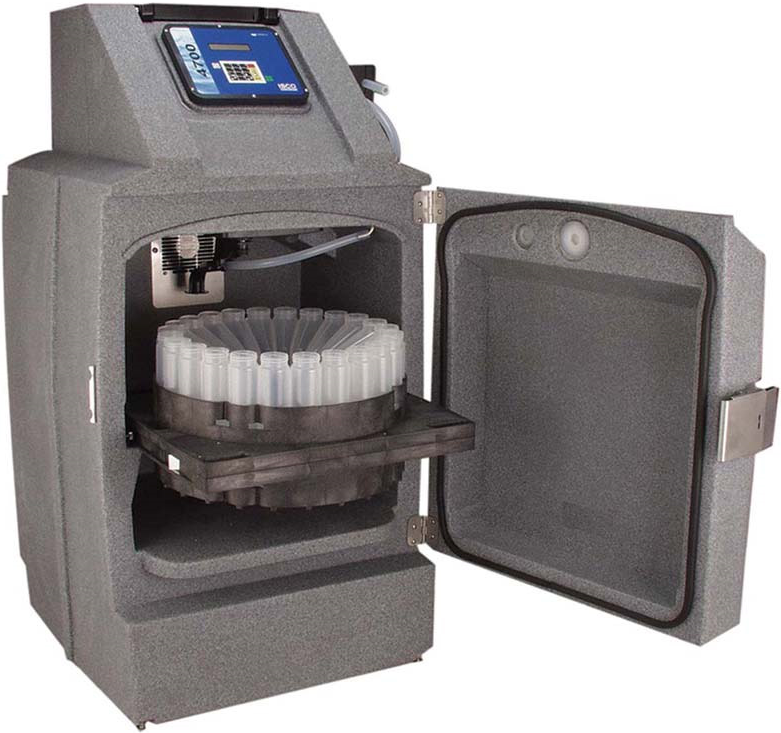
\includegraphics[scale=0.2]{Autosampler} \hspace{2cm} 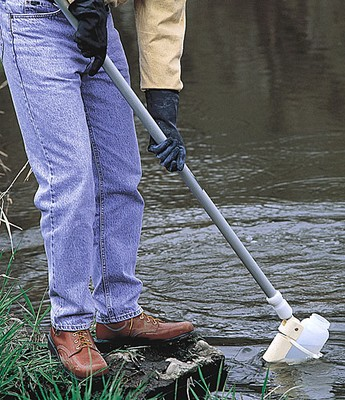
\includegraphics[scale=0.37]{Grabsampler}\\
			\end{center}
			\hspace{2.3cm} Automated Sampler \hspace{2.0cm} \parbox{\textwidth}{Grab Sampling Using a Long Handle Dipper}\\

\subsubsection{Sampling Precautions and Protocols}\index{Sampling Precautions and Protocols}
			\begin{itemize}
				\item Samples should represent the major portion of the process or the process stream and should be taken from places where the mixing is thorough, avoiding dead spots and areas of heavier or lighter loadings. 
				\item The collected sample is invariably exposed to conditions very different from the original source and is subject to change due to chemical and microbiological activity.  
				\item Thus, in order to ensure integrity of sample, sample preservation techniques specific to the analysis to be performed is needed.  
				      \begin{itemize}
				      	\item The preservation technique should not only allow for stabilizing the parameter to be analyzed, it should also not interfere with the analyses.  
				      	\item The common preservation techniques involve use of proper containers, temperature control, addition of chemical preservatives, and observance of the recommended maximum sample holding time.
				      \end{itemize}
			\end{itemize}
			
\subsubsection{Bacteriological Sampling}\index{Bacteriological Sampling}
\begin{itemize}
\item Always collected as a grab
\item A clean, sterile borosilicate glass or plastic bottle containing sodium thiosulfate is used. Sodium thiosulfate is added to remove residual chlorine which will kill coliforms during transit. If the sample is not preserved or maintained under proper conditions until the test is conducted in the laboratory, the test would provide erroneous results
\item Samples must be refrigerated if they cannot be analyzed within 1 hour of collection
\item Samples must be handled with care to prevent contamination and adverse conditions such as prolonged exposure to direct sunlight
\item Maximum holding time for state or federal permit reporting purposes is 6 hours
\end{itemize} 

\subsection{Data Reporting}\index{Data Reporting}	
		\begin{itemize}
			\item Arithmetic mean is typically calculated for reporting data where multiple samples have been collected and analyzed for the same process stream at different times and for reporting average value over a certain time period – daily, monthly etc.\\ \item Arithmetic mean mathematically is calculated by adding all the result values and dividing by the total number of data points.\\
		\end{itemize}
		Mathematically the arithmetic mean is represented as:\\
		$$\bar{x}=\frac{\sum_{i=1}^{n} x^i}{n} = \frac{x_1+x_2+x_3...x_n}{n}$$
		For example:\\
		Arithmetic mean of the following set of data points:  200, 304, 250, 400 is calculated as:\\
		\vspace{10pt}
		Arithmetic Mean = $\frac{200 + 302 + 250 + 400}{4}= 288$\\
		\vspace{10pt}
		For data sets for analysis such as fecal coliform could include values which vary by several orders of magnitudes, using the arithmetic mean to report the average value is not appropriate as the lower or higher values would bias the calculated mean.\\
		\vspace{10pt}
		For example, consider a data set with values:  260, 300, 500, 5,000, 320 and 200.\\
		\vspace{10pt}
		The arithmetic mean = $\frac{260+300+500+5,000+320+200}{6} = 3,444$\\
		Here the 5000 value completely skews the arithmetic mean.
		
		Therefore, for such tests, the geometric mean calculation is used for reporting the average value.\\
		
		
		Mathematically a geometric mean is represented as:\\
		$$\Bigg(\prod_{i=a}^n\Bigg)^{\frac{1}{n}}=\sqrt[n]{a_1*a_2*a_3...a_n}$$
		 
		Calculation method:\\
		1.	Find the product of all the data points (analogous to first calculating the sum of all the data points when calculating the arithmetic mean)\\
		260*300*500*5,000*320*200 = 12,480,000,000,000,000\\
		2.	Raise the product to the inverse of the number of data points\\
		(*Using the power function of a scientific calculator)\\
		Here n (\# data points) = 6 $\implies$ geometric mean = $(12,480,000,000,000,000)^{\frac{1}{6}}   = 482$

\section{Laboratory Analysis}\index{Laboratory Analysis}

		\subsection{BOD Analysis}\index{BOD Analysis}		
\begin{itemize}
\setlength\itemsep{1em}

\item The Biochemical Oxygen Demand (BOD) test estimates the amount of biodegradable material present by measuring the amount of oxygen used by the bacteria to break down the organic waste in the sample incubated at 20 deg. C over a five-day period . The BOD test provides an indication on the strength of wastewater in terms of how much oxygen could be depleted if that wastewater was introduced into another receiving water.  Complete stabilization of a sample may require a period of incubation too long for practical purposes; therefore, 5 days has been accepted as the standard incubation period.

\item As the regular BOD test includes estimation of oxygen nitrifying bacteria consumes in the process of converting inorganic forms of ammonia and nitrogen to nitrite and nitrate, its value represents oxygen used for removing both, organic material and nitrogenous matter.  As this BOD value does not quite represent the organic strength of the wastewater, the normal BOD test is modified by introducing a chemical inhibitor - 3 mg of 2-chloro-6-(trichloro methyl) pyridine (TCMP), which suppresses the growth of the nitrogenous bacteria so that the resultant BOD measured represents the oxygen depletion associated with the depletion of the organic matter only.  This is the Carbonaceous biochemical oxygen demand or cBOD. \\
\vspace{0.4cm}
\textbf{Thus tBOD = nBOD + cBOD}

\item Wastewater BOD measurement involves testing a sample set consisting of several sample dilutions along with a "Blank".  "Blank" is a sample with only the dilution water with no wastewater added. \\


\item The dilutions are made based upon the expected BOD concentration of the sample.  Using the final dilution volume of 300 ml, the initial sample volume can be estimated using the formula:\\

\textbf{$Sample \enspace Volume (ml) = \dfrac{\Big[Oxygen \enspace Depletion \Big(\dfrac{mg}{l}\Big)\Big]}{Anticipated \enspace BOD \Big(\dfrac{mg}{l}\Big)}*300 \enspace ml$}\\

\item For example, if testing an influent wastewater BOD with an expected BOD value of 250 mg/l, a range of sample volumes for dilution around sample volume of $\dfrac{4\dfrac{mg}{l}}{250 \dfrac{mg}{l}}*300 \enspace ml$=5ml.\\
\vspace{0.4cm}
\item The data obtained for each of the dilutions after the 5-day incubation period must meet the following criteria for the sample value to be acceptable for calculating the BOD.\\
\vspace{0.4cm}

\begin{enumerate}[1.]
\setlength\itemsep{1em}

\item A residual DO of at least 1 mg/L,
\item A DO depletion of at least 2 mg/L
\end{enumerate}
\vspace{0.4cm}
\item Additionally, the whole sample set is rejected if the Blank shows an oxygen depletion of >0.2mg/l.\\
\vspace{0.4cm}
\item BOD is calculated for each sample dilution value using the following formula:\\
\vspace{0.4cm}
\textbf{$BOD \Big(\dfrac{mg}{l}\Big) = \dfrac{Initial \enspace DO - DO \enspace Day \enspace 5}{Sample \enspace Volume \enspace (ml)}*300 \enspace ml$}\\



\end{itemize}
\vspace{0.4cm}
\subsection{Wastewater solids}\index{Wastewater solids}

	\subsubsection{Total (TSS) and Volatile (VSS)}\index{Total (TSS) and Volatile (VSS)}
\begin{itemize}
\setlength\itemsep{1em}
					\item A known volume of wastewater sample is filtered through a pre-weighed filter paper
					\item The suspended solids will be retained by the filter
					\item The water with the dissolved solids will pass through the filter
					\item The filter paper with the filter solids is rinsed with distilled water to remove 
					\item The filter paper with the solids is dried in the oven and then weighed
					\item The difference between the weight of the dried filter paper with the solids and the pre-weighed filter paper, measured in mg, will be the suspended solids in: mg per the original quantity of wastewater sample taken.  This value can be converted to give the suspended solids content in mg/l
					\item A filter paper with the dried solids is incinerated in a muffler furnace
					\item The difference in the weight of the solids, before and after incineration is the fixed solids
					\item The difference between the weight of the solids before incineration and the fixed solids is the volatile solids
	\end{itemize}				

\textbf{Total Suspended Solids - TSS}
\vspace{0.4cm}
$TSS \dfrac{mg}{l}=\dfrac{weight \enspace of \enspace solids \enspace \cancel{gms}}{volume \enspace of \enspace sample \enspace \enspace \cancel{ml}}*\dfrac{1000 \enspace \cancel{ml}}{l}*\dfrac{1000 \enspace mg}{\cancel{gms}}$\\
\vspace{0.3cm}
\hspace{1.4cm}$=\dfrac{weight \enspace of \enspace filter \enspace paper  \enspace with \enspace dried  \enspace solids - weight \enspace of \enspace filter \enspace paper}{volume \enspace of \enspace sample \enspace \enspace (ml)}*1,000,000$\\
\vspace{0.4cm}

\vspace{0.4cm}
\textbf{Volatile Suspended Solids - VSS}	
\vspace{0.4cm}

$VSS \dfrac{mg}{l}=\dfrac{weight \enspace of \enspace volatile \enspace solids \enspace \cancel{gms}}{volume \enspace of \enspace sample \enspace \enspace \cancel{ml}}*\dfrac{1000 \enspace \cancel{ml}}{l}*\dfrac{1000 \enspace mg}{\cancel{gms}}$\\
\vspace{0.3cm}
\hspace{1.4cm}$=\dfrac{wt. \enspace of \enspace filter \enspace paper  \enspace with \enspace dried  \enspace solids - wt. \enspace of \enspace filter \enspace paper \enspace incinerated \enspace residue}{volume \enspace of \enspace sample \enspace \enspace (ml)}*1,000,000$\\
\vspace{0.3cm}
$VSS(\%)=\dfrac{weight \enspace (gms) \enspace of \enspace volatile \enspace solids}{100 \enspace gms \enspace total \enspace solids}=\dfrac{gms \enspace volatile \enspace solids}{\cancel{gms \enspace total \enspace solids}}*\dfrac{100 \cancel{\enspace gms \enspace total \enspace solids}}{100 \enspace gms \enspace total \enspace solids}$\\
\vspace{0.3cm}
\hspace{1.5cm}\small{$=\dfrac{wt. \enspace of \enspace filter \enspace paper  \enspace with \enspace dried  \enspace solids - wt. \enspace of \enspace filter \enspace paper \enspace incinerated \enspace residue}{wt. \enspace of \enspace filter \enspace paper  \enspace with \enspace dried  \enspace solids - wt. \enspace of \enspace filter \enspace paper}*100$}\\				

	\subsubsection{Wastewater and Sludge Total \& Volatile Solids}\index{Wastewater and Sludge Total \& Volatile Solids}
\vspace{0.4cm}
\begin{itemize}
\setlength\itemsep{1em}
					\item A certain quantity of wastewater (by volume) or sludge (by weight) is taken in a pre-weighed dish and weighed.  \hl{Note:  the sample is not filtered.}
					\item The dish with the sample is dried in an oven
					\item The difference in the weight of the pre-weighed dish from that of the dish with the dried sample is the total solids
					\item The dried solids are incinerated in a muffler furnace
					\item The difference in the weight of the solids, before and after incineration is the fixed solids
					\item The difference between the fixed solids and the total solids is the volatile solids
					\item Total solids of a sludge sample is reported as a \% of the sludge weight.  A 7\% sludge has 7 lbs of solids for every 100 lbs of sludge.
				\end{itemize}
				
				\hl{For sludge samples, volatile solids is typically reported as the volatile solids fraction in \% of the total solids content of the sludge.  For example, if a 8\% sludge (i.e sludge which has 8\% TS or 80,000mg/l solids), is reported to have 70\% volatile, it means that 70\% of the total solids - 0.7*8\%=5.6\% or 56,000mg/l is the sludge volatile solids content.  \emph{70\% volatile does not meet the sludge has 700,000mg/l volatile solids}}\\	

\vspace{0.4cm}
\textbf{Total Solids - TS}			
\vspace{0.4cm}
$TS(\%)=\dfrac{weight \enspace of \enspace solids \enspace (gms)}{100 \enspace gms \enspace of \enspace sample}=\dfrac{gms \enspace solids}{gms \enspace sample}*100$\\
\vspace{0.3cm}
\hspace{1.2cm}$=\dfrac{weight \enspace of \enspace cruicible \enspace with \enspace dried  \enspace solids - weight \enspace of cruicible}{weight \enspace of \enspace cruicible \enspace with \enspace sample - weight \enspace of cruicible}*100$\\
\vspace{0.4cm}
\textbf{Total Volatile Solids - VS}		
\vspace{0.4cm}
$VS(\%)=\dfrac{weight \enspace of \enspace volatile \enspace solids \enspace (gms)}{100 \enspace gms \enspace of \enspace total \enspace solids}=\dfrac{gms \enspace volatile \enspace solids}{gms \enspace total \enspace solids}*100$\\
\vspace{0.3cm}
\hspace{1.2cm}$=\dfrac{wt. \enspace of \enspace cruicible  \enspace with \enspace dried  \enspace solids - wt. \enspace of \enspace cruicible \enspace incinerated \enspace residue}{wt. \enspace of \enspace cruicible  \enspace with \enspace dried  \enspace solids - wt. \enspace of \enspace cruicible}*100$\\

\newpage
\thispagestyle{empty}
% \begin{landscape}
% \begin{center}
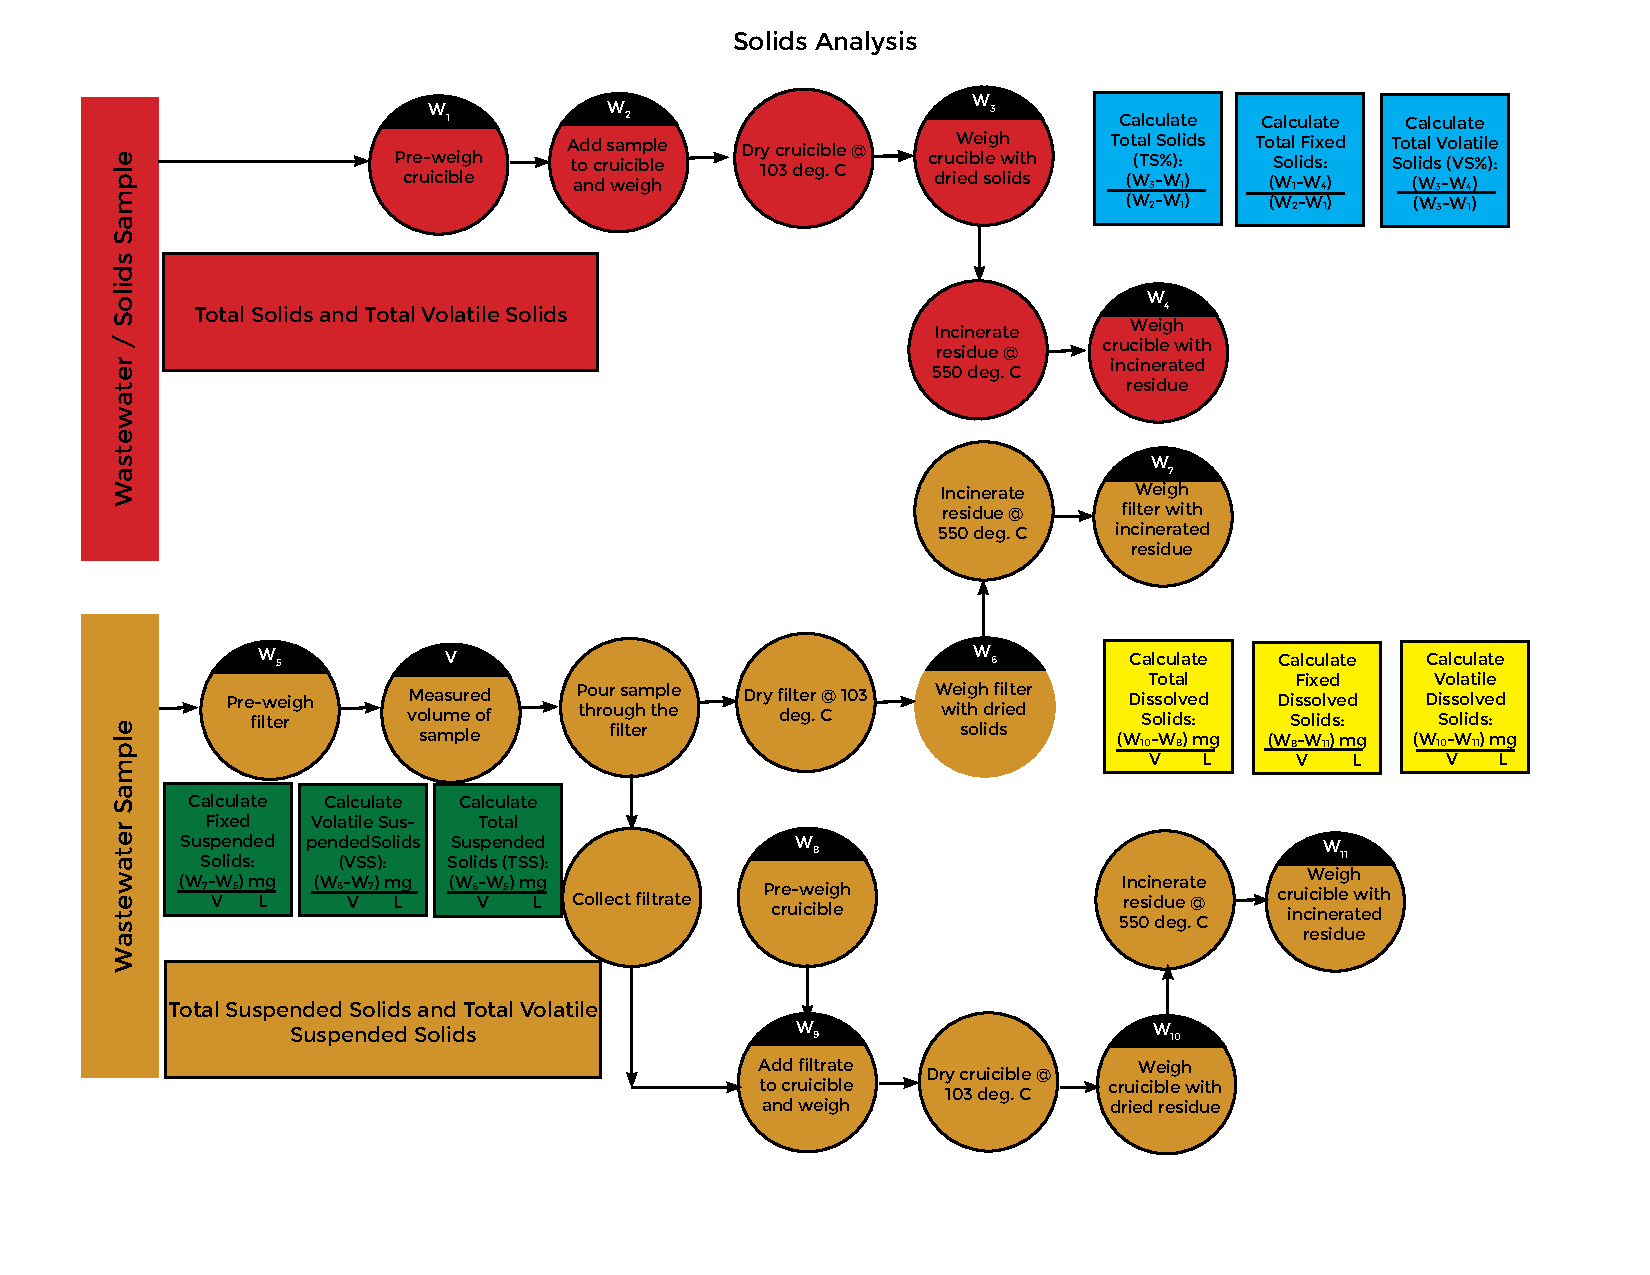
\includepdf[landscape=true]{LaboratorySolidsAnalysis4_01.pdf}
				\newpage
				\thispagestyle{empty}
				\begin{sidewaysfigure}
					\begin{center}
						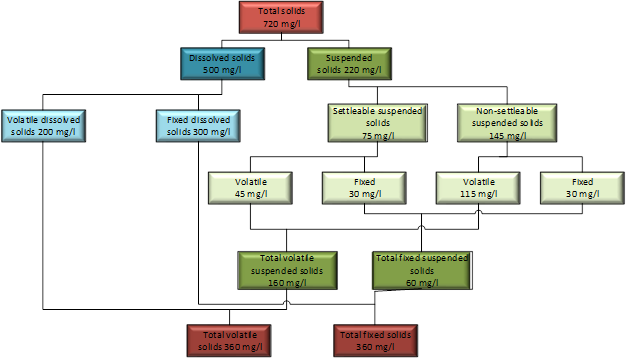
\includegraphics[scale=1.0]{WastewaterSolids}\\
						\caption{Typical Wastewater Solids Concentrations}
					\end{center}
				\end{sidewaysfigure}
%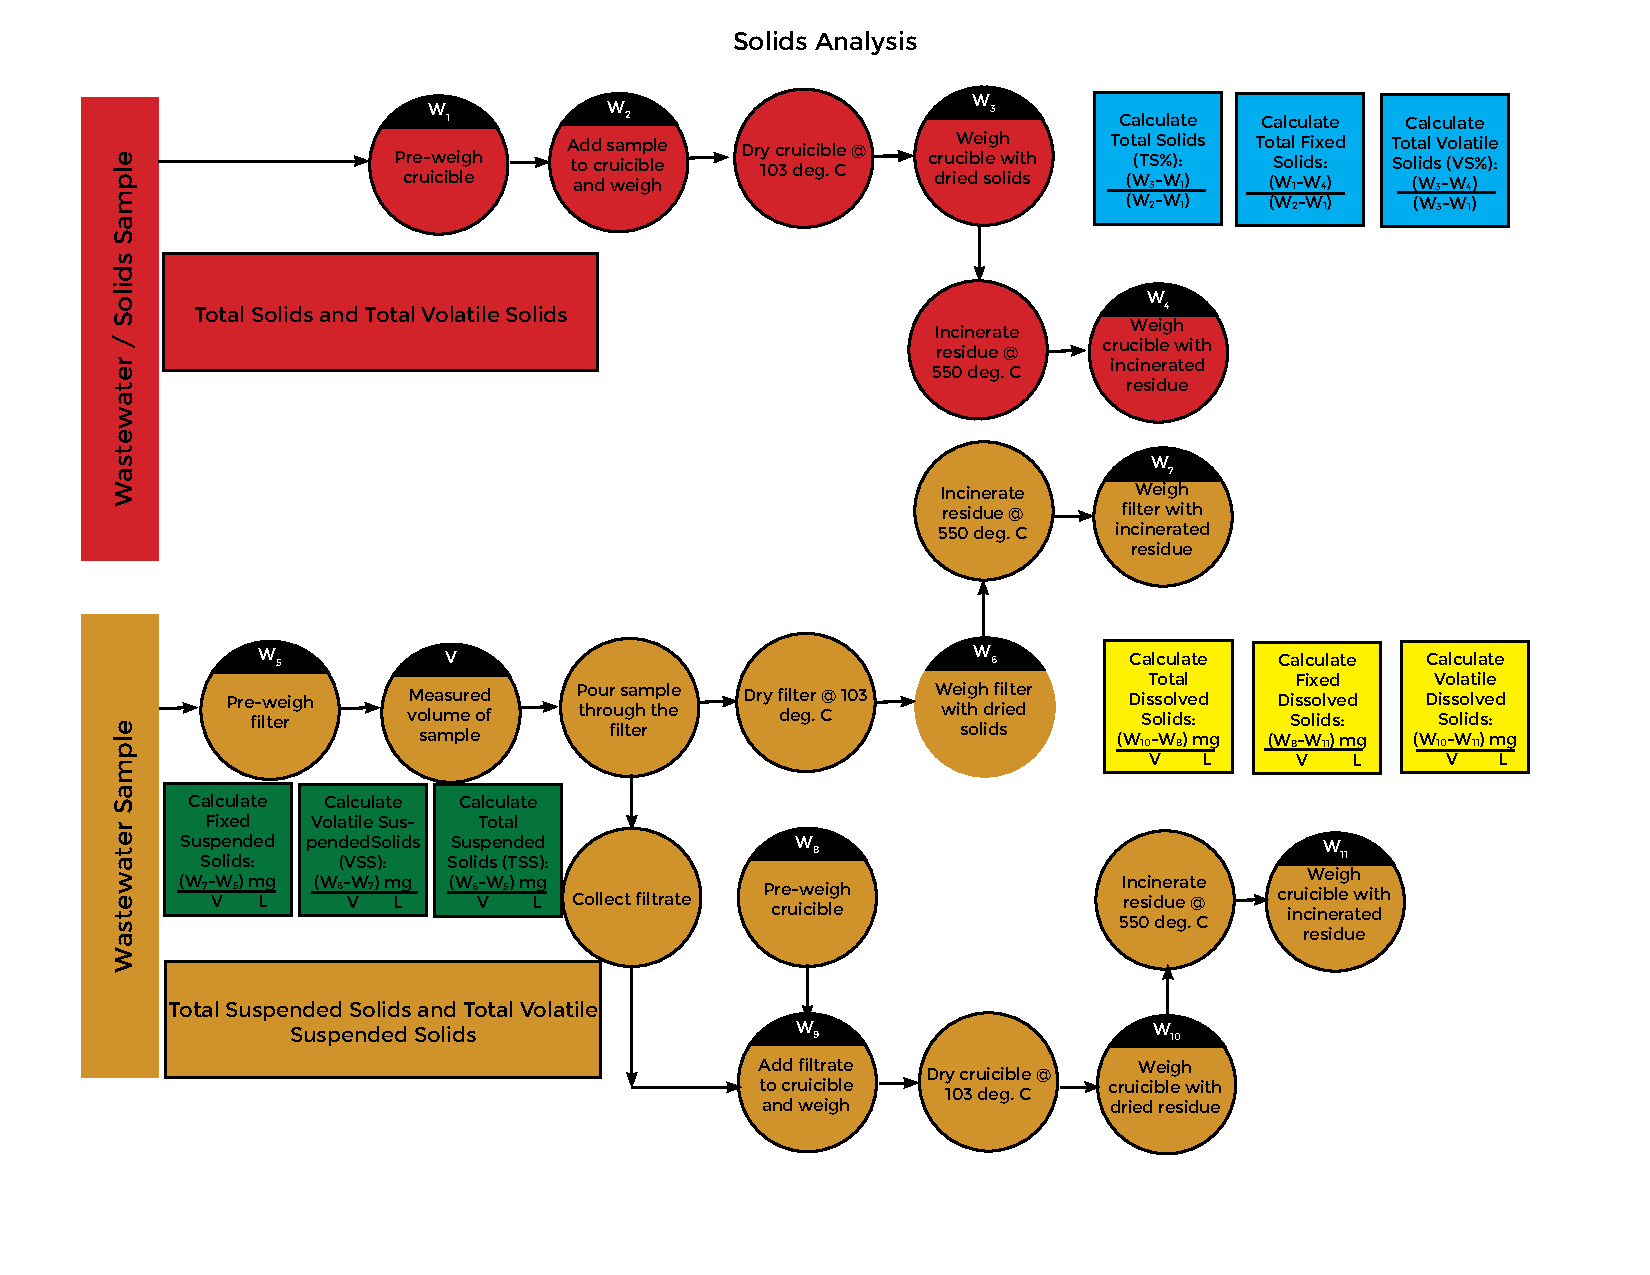
\includegraphics[scale=0.69]{LaboratorySolidsAnalysis4_01.pdf}
% \end{center}
% \end{landscape}
\subsubsection{Sample BOD and solids analysis math problems}\index{Sample BOD and solids analysis math problems}
\begin{enumerate}
\item BOD tests are run on the final effluent from an activated sludge plant with and without the use of a "nitrification inhibitor". Three hundred milliliter bottles (300 ml) are used in these tests. The raw data for these tests are presented below.  What \textbf{percentage of the average total BOD is the average nBOD}?\\
\vspace{0.5cm}
\begin{tabular}{m {4 cm} m {1.5 cm} m  {1.5 cm} m  {1.5 cm} m  {1.5 cm} m {1.5 cm}}
\cline{1-6}
Sample Volume, ml    & 10 & 20 & 30 & 40 & Blank\\
\hline
Initial DO, mg/l 			& 9.0 	& 	8.9 & 8.8  & 9.1 & 9.1\\
Final DO, mg/l 			& 6.9 	& 	4.8 & 2.5 & 1.1 & 9.0
\end{tabular}
\vspace{0.7cm}\\
BOD Test with "inhibitor" added	(cBOD)\\
\vspace{0.5cm}
\begin{tabular}{m {4 cm} m {1.5 cm} m  {1.5 cm} m  {1.5 cm} m  {1.5 cm} m {1.5 cm}}
\cline{1-6}
Sample Volume, ml    & 10 & 20 & 30 & 40 & Blank\\
\hline
Initial DO, mg/l 			& 8.9 	& 	8.9 & 9.0  & 9.0 & 9.1\\
Final DO, mg/l 			& 7.5 	& 	6.2 & 5.0 & 3.3 & 9.0
\end{tabular}
\vspace{0.5cm}\\
Solution:\\
Blanks for both tBOD and cBOD are both <=0.2mg/l - thus sample sets are acceptable\\
\vspace{0.5cm}
\begin{tabular}{m {3 cm} m {2.5 cm} m  {2.5 cm} m  {2.5 cm} m  {2.5 cm} }
\cline{1-5}
Sample Volume, ml    & 10 & 20 & 30 & 40 \\
\hline
tBOD Diff., mg/l    & 2.1 & 4.1 & 6.3 & 8 \\
tBOD, mg/l    & 2.1*300/10 & 4.1*300/20 & 6.3*300/30 & 8.0*300/40\\
    & =63.0 & = 61.5  & = 63.0 & = 60.0 \\
\hline
cBOD Diff., mg/l    & 1.4 & 2.7 & 4.0 & 5.7 \\
cBOD, mg/l    & Reject & 2.7*300/20 & 4.0*300/30 & 5.7*300/40\\
    & Depletion < 2 & = 40.5  & = 40 & = 42.75 \\
\end{tabular}
\vspace{0.5cm}\\

$tBOD (avg) = (63+61.5+63+60)/4=61.9 \hspace{1cm} cBOD (avg) = (40.5+40+42.75)/3=41.1$\\
nBOD = tBOD - cBOD $\implies$ nBOD = 61.9-41.1=20.8 $\implies$ nBOD(\%)=20.8/61.9*100=$\boxed{33.6\%}$
\vspace{0.5cm}
\item Calculate percent total solids and percent volatile solids of a sludge sample given the following data:\\
\begin{tabular}{m {5 cm} m {0.5 cm} m  {3.5 cm}}
Weight of dish &=&  104.55 gms\\
Weight of dish and wet sludge &= & 199.95 gms\\
Weight of dish and dry sludge &= & 108.34 gms\\
Weight of dish and ash &= & 106.37 gms
\end{tabular}\\
\vspace{0.2cm}
Solution:\\
\vspace{0.2cm}
Weight of dish=104.55 gms\\
Weight of dish and wet sludge=199.95 gms\\
Weight of dish and ash = 106.37 gms\\
\vspace{0.2cm}
$ \implies Weight \enspace of \enspace sludge=199.95-104.55=95.40 \enspace gms$\\
$\implies Weight \enspace of \enspace dry \enspace sludge \enspace (solids)=108.34-104.55=3.79 \enspace gms$\\
$\implies Weight \enspace of \enspace volatile \enspace solids=108.34-106.37=1.97 \enspace gms$\\
\vspace{0.2cm}
$Total \enspace solids (TS\%)=\dfrac{gms \enspace solids}{100 \enspace gms \enspace sludge}=\dfrac{3.79}{95.40} \enspace \dfrac{gms \enspace solids}{\cancel{gms \enspace sludge}}*\dfrac{100 \cancel{\enspace gms \enspace sludge}}{100 \enspace gms \enspace sludge}=\boxed{3.97\%}$\\
\vspace{0.2cm}
$Total \enspace volatile \enspace solids (VS\%) =\dfrac{1.97}{3.79} \enspace \dfrac{gms \enspace volatile \enspace solids}{\cancel{gms \enspace total \enspace solids}}*\dfrac{100 \cancel{\enspace gms \enspace total \enspace solids}}{100 \enspace gms \enspace total \enspace solids}=\boxed{52.0\%}$\\


\end{enumerate}

\subsection{Bacteriological Ennumeration}\index{Bacteriological Ennumeration}

\begin{tabular}{|c||l|}
\hline
\multicolumn{1}{|c|}{Pathogen} & \multicolumn{1}{c|}{Disease Caused} \\
\hline
Bacteria: &  \\
\hline\hline
Anthrax & anthrax \\
\hline\hline
Escherichia coli & E. coli infection \\
\hline\hline
Myobacterium & tuberculosis \\
tuberculosis &  \\
\hline\hline
Salmonella & salmonellosis, \\
paratyphoid &  \\
\hline\hline
Vibrio cholerae & cholera \\
\hline\hline
Viruses: &  \\
\hline\hline
Hepatitis Virus & Hepatitis A \\
\hline\hline
Polio Virus & polio \\
\hline\hline
Parasites: &  \\
\hline\hline
Cryptosporidium & cryptosporidiosis \\
\hline\hline
Giardia lamblia & giardiasis \\
\hline\hline
\end{tabular}

\begin{itemize}
	\item Involves bacteriological testing of the wastewater effluent and the surface water impacted by the wastewater discharge
	
	\item Conducted in-order to:
		\begin{enumerate}
			\item Meet the requirements of a wastewater discharge permit
			\item Monitor the pathogen impact of treated wastewater discharge
			\item Assess the level of contamination of a public body of water
			\item Bacteriological tests involves detection and quantification of one or more of the following bacteria:  total coliforms, fecal coliforms, \textit{E. Coli}, and \textit{Enterococci}. 
\begin{center}
\tcbox{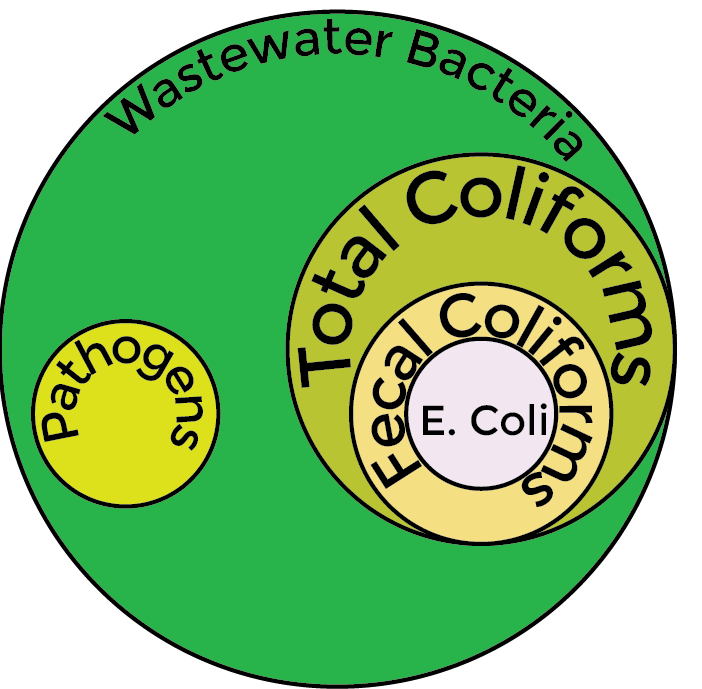
\includegraphics[width=4cm]{LaboratoryWastewaterBacteria}}
Wastewater Bacteria
\end{center}
	
	\item  In wastewater, fecal coliforms originate in the intestines of warm-blooded animals.  Aerobic bacteria including coliforms partake in the metabolization of the organic matter as part of the secondary treatment process
\item Fecal coliforms are seldom pathogenic under normal circumstances and are easily cultured, their presence indicates the potential presence of pathogens

The reason why these bacteria such as coliforms and enterococcus are used:
		\begin{enumerate}
			\item It is not practical to detect and quantify all pathogens associated with wastewater
			\item These bacteria originate from feces and indicate fecal contamination and thus serve as an indicator organisms for pathogens of wastewater origin
			\item They are also:
				\begin{itemize}
					\item abundant
					\item potentially less harmful, and
					\item easy to detect
				\end{itemize}
			\item \textit{E. coli} has been shown to be a better predictor of the potential for impacts to human health and therefore many newer wastewater discharge permits require \textit{E. Coli} testing in lieu of fecal coliform testing requirements.
		\end{enumerate}
		\end{enumerate}

\end{itemize}
 

\subsubsection{Bacteriological Testing Methods}\index{Bacteriological Testing Methods}
The methods for wastewater bacteriological tests include:  multiple-tube fermentation (MTF) technique, membrane filtration (MF) and quanti-tray testing.  When using the MTF and MF methods, it is not possible to exactly quantify the number of bacteria present, a statistical based - Most Probable Number (MPN) approach is utilized\\
\subsubsection{The Multiple-Tube Fermentation (MTF) technique}\index{The Multiple-Tube Fermentation (MTF) technique}
This involves adding three volumes – 10 ml, 1 ml and 0.1 ml of the sample, each to a set of five tubes containing Lauryl Tryptose broth and an inverted tube (Durham tube), followed by incubating the tubes at  for a specified time.  The Lauryl Tryptose broth produces color and/or turbidity change due to the growth of the target bacteria and the inverted tube collects the gas produced by the bacterial respiration.  At the end of the process, the number of tubes showing bacterial growth are counted for each volume of sample and using this information the concentrations of organisms in the original sample are established using Statistical Tables.  The test is conducted in three parts – presumptive, confirmative and completed.  A schematic of the MTF used for quantifying total coliforms and fecal coliforms is provided below.\\
\newpage
\thispagestyle{empty}
% \begin{landscape}
% \begin{center}
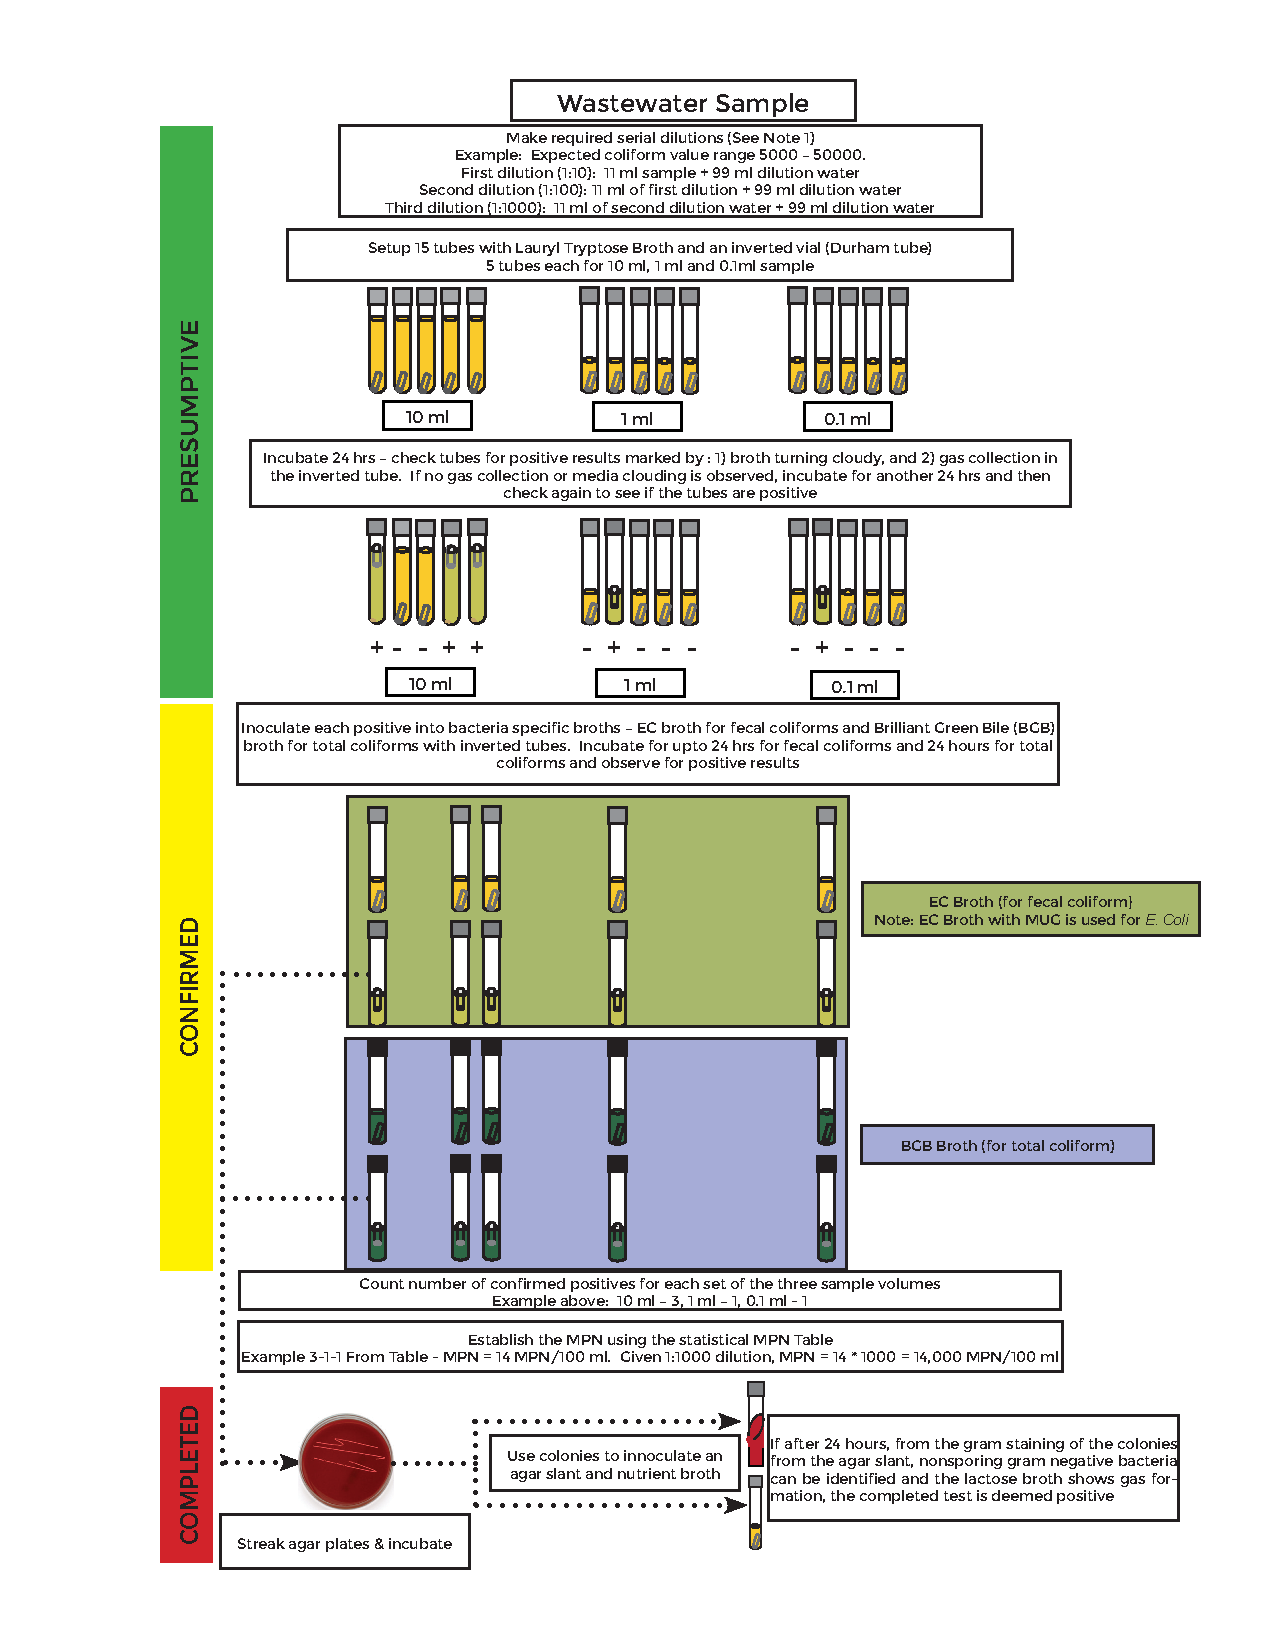
\includepdf[]{MTF.pdf}
%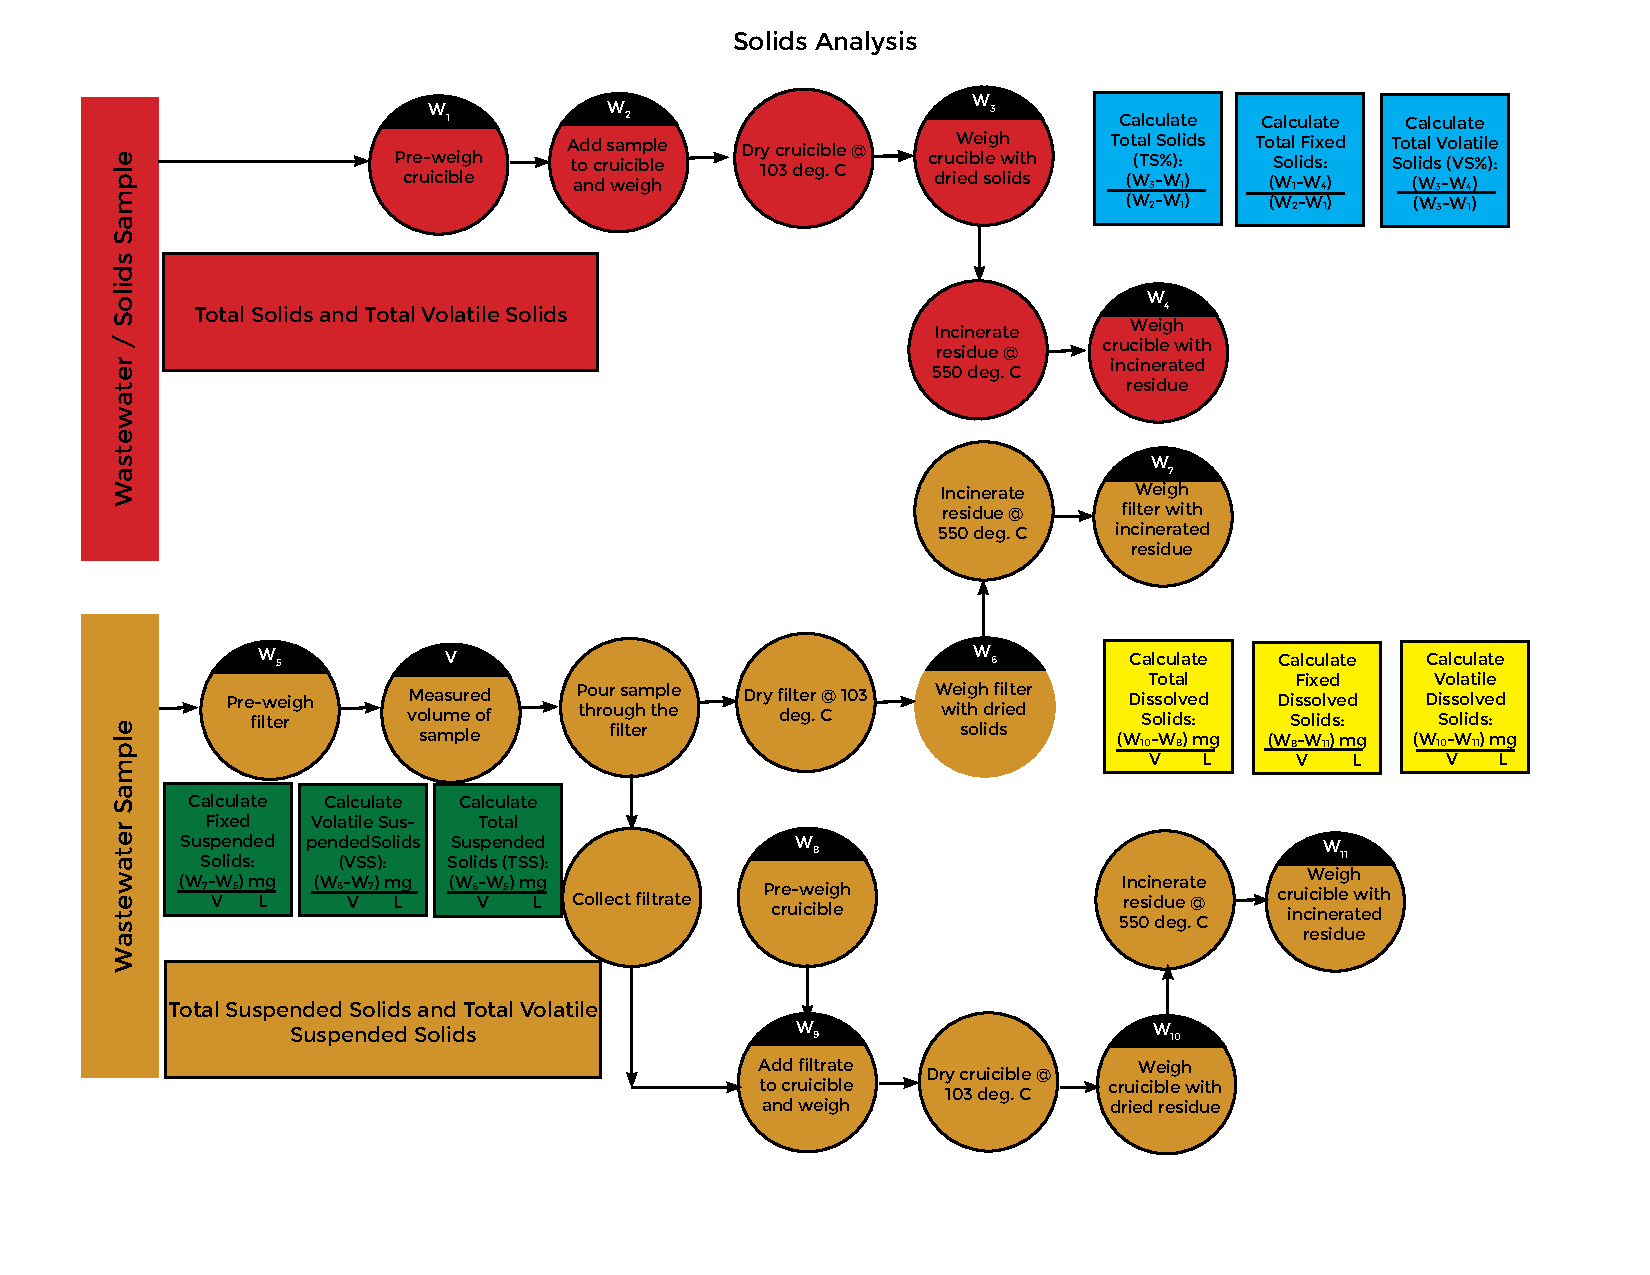
\includegraphics[scale=0.69]{LaboratorySolidsAnalysis4_01.pdf}
% \end{center}
% \end{landscape}
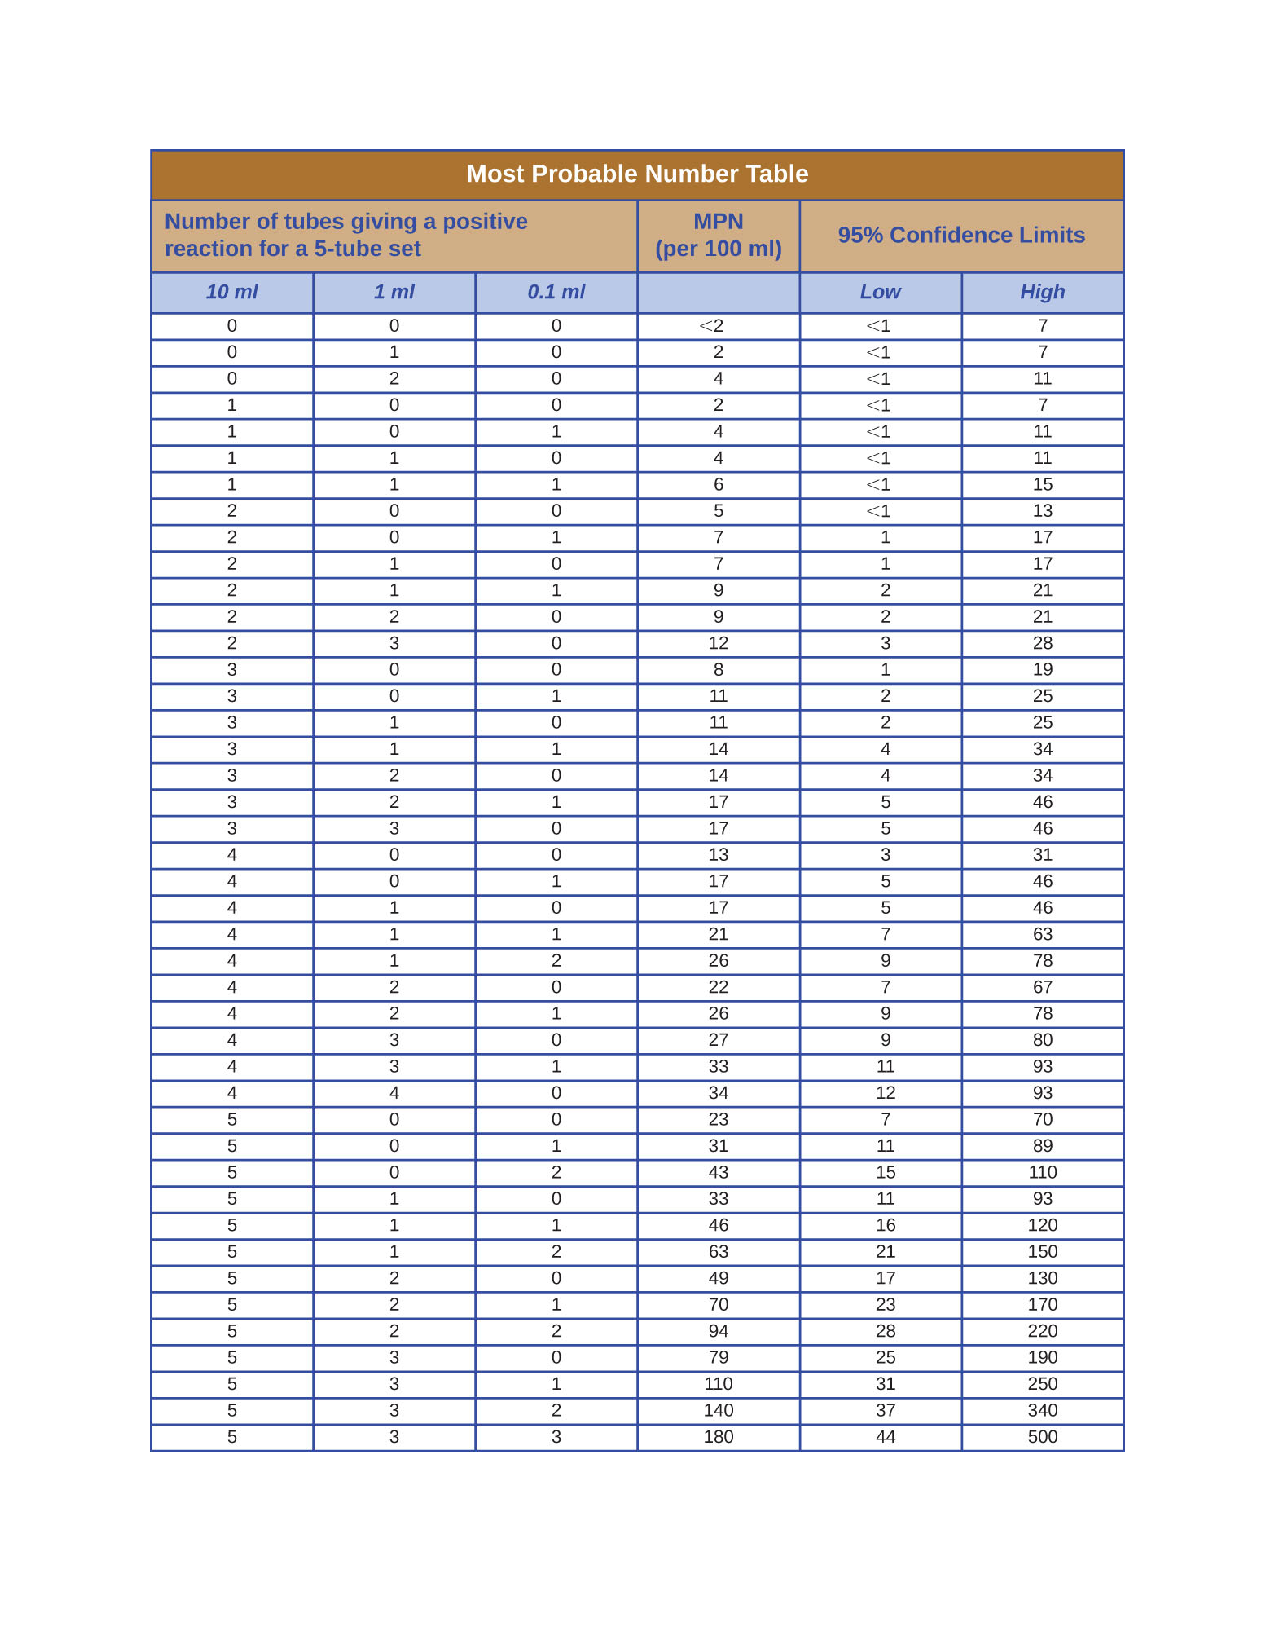
\includepdf[]{MTFTable.pdf}
\newpage
\subsubsection{The Membrane Filtration (MF) method}\index{The Membrane Filtration (MF) method}
This is a faster way to estimate bacterial populations in water.  In this method, an appropriate sample volume is passed through a membrane filter with a pore size small enough (0.45 micron) to retain the bacteria present. The filter is placed on an absorbent pad (in a petri dish) saturated with a culture medium that is selective for coliform growth. The petri dish containing the filter and pad is incubated, upside down, for 24 hours at the appropriate temperature. After incubation, the colonies that have grown are identified and counted using a low power microscope. A MUG medium is used for E- Coli.  If E. Coli is present, it will make the MUG fluorescent when viewed in UV light. 
\begin{center}
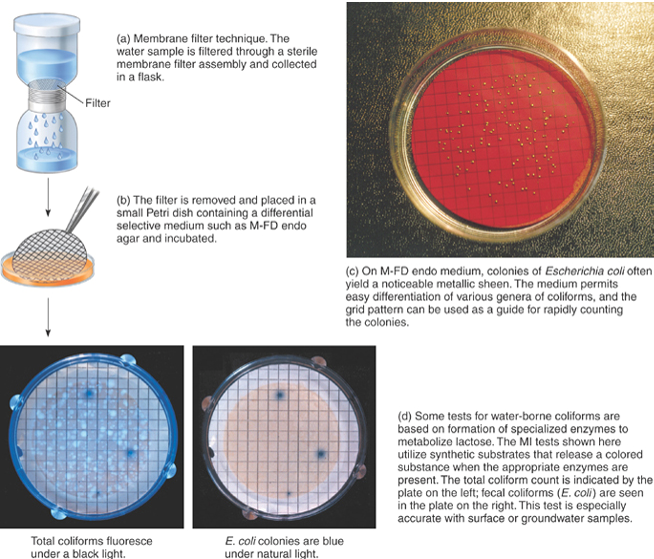
\includegraphics[scale=0.9]{LaboratoryMembraneFiltration}
\end{center}
\pagebreak

\subsubsection{Quanti-trays tests}\index{Quanti-trays tests}

This test used for the detection and quantification of specific microorganisms is being used increasingly mainly because it is a quicker test than the MTF.  Colilert and Enterolert are the quanti tray based tests for E. Coli and Enterococcus.  This method involve the use of specific enzymes and overcomes the drawbacks of the MTF which include false positives and negatives due to the more generic nature of the media used
\begin{center}
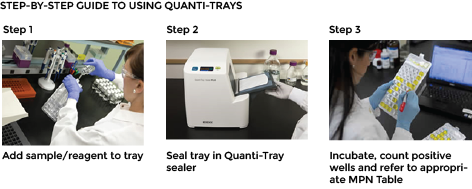
\includegraphics[scale=0.9]{LaboratoryQuantiTray}
\end{center}




%\chapterimage{ElementsofTreatmentImg.png} % Chapter heading image
\chapter{Elements of Wastewater Treatment}

Wastewater cycle is a part of the water cycle where the water consumed as part of the normal human and industrial activity is returned back to the environment after treatment.

Wastewater cycle comprises of the following sequential elements:
\begin{enumerate}
\item Generation
\item Collection
\item Treatment
\item Disposal or reuse
\end{enumerate}

\section{Generation}\index{Generation}

Wastewater originates from domestic, industrial, commercial or agricultural activities. The characteristics of wastewater vary depending on the source. Types of wastewater include: 
\begin{itemize}
\item \hl{Domestic Sewage:}  wastewater derived principally from dwellings, business buildings, institutions, and \\
\item \hl{Industrial Sewage:}  liquid waste from industrial processes\\
\end{itemize}
Typical per person generation of wastewater in the USA is about 70-100 gallons per day

\section{Collections}\index{Collections}

\begin{itemize}
\item Wastewater is collected from its point of origin - home, businesses, industries etc. and conveyed via sewer lines to a centralized wastewater treatment facility.  
\item When the rainwater drainage is made part of the sewer system, the system is termed as \hl{Combined System}.  
\item The system where the sewage is conveyed separately from the stormwater flows is termed as \hl{Separated System}.  
\item In the Separated System, the Sanitary Sewers convey the wastewater and the Stormwater Sewer conveys the storm water flows.  
\item For the Combined System, rainstorms pose the threat of overwhelming the sewers and the treatment plant
\end{itemize}  
\begin{center}
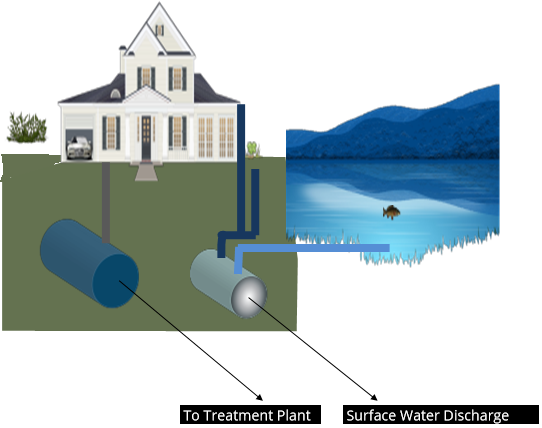
\includegraphics[scale=0.45]{SeperatedSystem1} \hspace{1 cm} 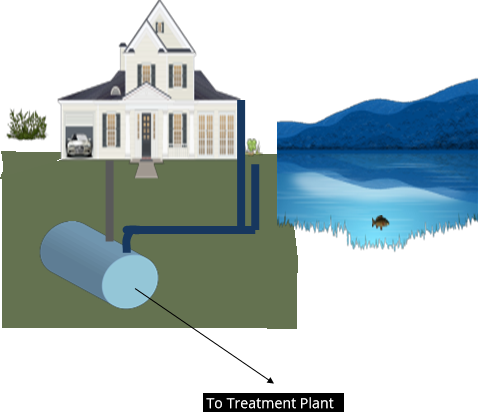
\includegraphics[scale=0.45]{CombinedSystem1}
\end{center}
			\hspace{2.6cm} Separated System \hspace{3.2cm} \parbox{\textwidth}{Combined System}\\

\section{Treatment}\index{Treatment}
\subsection{Liquid Phase Treatment}\index{Liquid Phase Treatment}
\begin{itemize}
\item Wastewater treatment can involve physical, chemical or biological processes or combinations of these processes depending on the required outflow standards. 
\item Wastewater treatment typically involves a series of steps with increasing level of treatment:
\begin{itemize}
\item \hl{Preliminary}:  The preliminary process removes large/coarse solids which include rocks, tree branches, grit and other debris present in wastewater.
\item \hl{Primary}:  The primary process is also a physical process where the separable wastewater solids - solids that float and solids that can settle, are removed.  
\item \hl{Secondary}:  Secondary treatment is a biological treatment process where microorganisms consume the organic matter present in the wastewater. 
\item \hl{Tertiary or Advanced Treatment}:  The tertiary/advanced treatment processes improve the quality of treated water beyond the secondary treatment level.  This process may include nutrient removal and disinfection.
\end{itemize}

\subsection{Treatment of Wastewater Solids}\index{Treatment of Wastewater Solids}
\begin{itemize}
\item Solids are a byproduct of wastewater treatment.  
\item Screenings and grit removed as part of the preliminary treatment is typically disposed in a landfill.
\item Sludge generated from the wastewater treatment processes -  settled solids and scum from primary and secondary treatment processes needs to be treated prior to disposal or reuse to comply with wastewater solids - biosolids regulations.
\end{itemize}

\vspace{0.5cm}
Typical solids treatment is comprised of the following three sequential steps:
\begin{enumerate}
\item Sludge thickening
\item Sludge stabilization
\item Sludge dewatering
\end{enumerate}
\vspace{0.5cm}
\subsubsection{Sludge Thickening}\index{Sludge thickening}
Sludge thickening improves performance of sludge stabilization process and provides capital and operational cost savings due to a lower volume of sludge
\subsubsection{Sludge Stabilization}\index{Sludge Stabilization}
Sludge stabilization process produces solids (biosolids) that meet Part 503 rule requirements. 
\subsubsection{Sludge Dewatering}\index{Sludge Dewatering}
Solids stabilized using digestion process has only a small percentage by weight of solids -less than 5\%.  It therefore becomes necessary to dewater the stabilized sludge prior to hauling off-site for final disposal. 
\vspace{0.5cm}
A generalized layout/process sequencing in a wastewater treatment plant is shown below:
\begin{center}
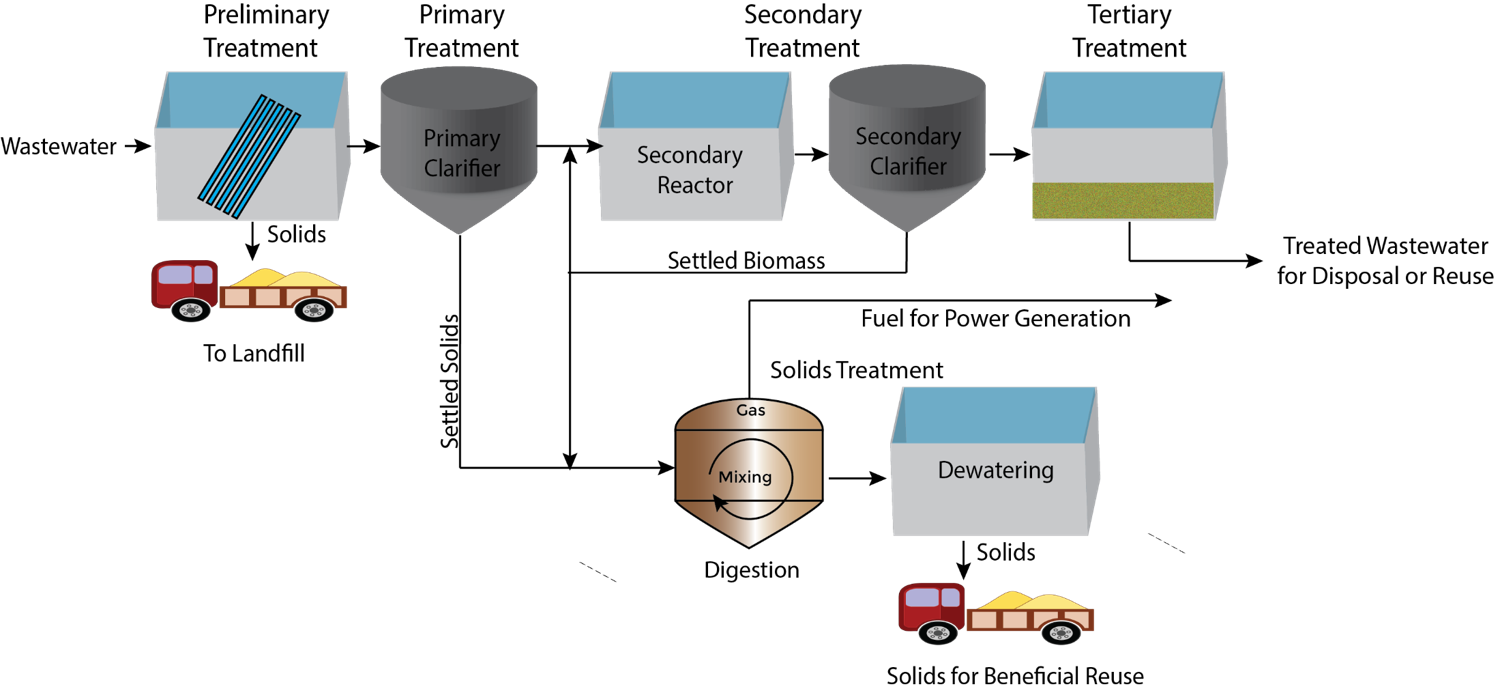
\includegraphics[scale=0.6]{TreatmentFlow}
\end{center}
Individual wastewater treatment processes involve different process options or sequences which are illustrated in the graphic below:
\begin{center}
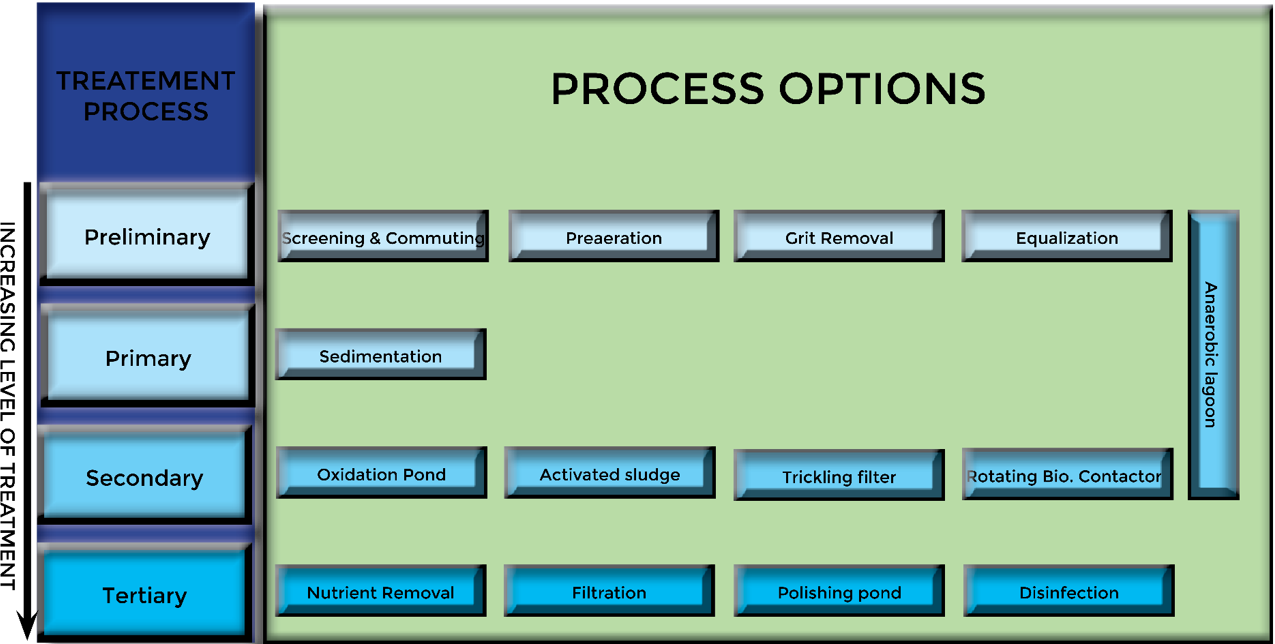
\includegraphics[scale=0.42]{Treatment}
\end{center}
\end{itemize}

\section{Disposal or Reuse}\index{Disposal or Reuse}

\begin{itemize}
\item Wastewater treatment processes can be designed to \hl{dispose} the treated water where the water is reintroduced to the environment or for \hl{reuse} where the treated water is \hl{reclaimed} or \hl{recycled} - for various purposes including irrigation, industrial use or for potable use.
\item Water disposal methods include:\\
\begin{itemize}
\item \hl{Surface water discharge}
\item \hl{Subsurface discharge}
\end{itemize}
\item Water reuse methods include:\\
\begin{itemize}
\item Potable water reuse
\begin{itemize}
\item \hl{Indirect potable reuse:}  Here the treated water is blended with groundwater or surface water and then reclaimed and treated further 
for drinking (potable) water use
\item \hl{Direct potable reuse:}  Here the treated wastewater is subjected to advanced treatment and introduced directly into a municipal water supply system
\end{itemize}
\item Water reclamation for irrigation or industrial use\\
\item Land application for beneficial use\\
\end{itemize}
\item Solids generated from the wastewater treatment process may be removed and disposed to a landfill or subject to further treatment which may allow for energy recovery - from the organic solids and for beneficial reuse due to its plant nutrient content.\\
\end{itemize}


%% \documentclass{article}
% %\usepackage[english]{babel}%
% \usepackage{graphicx}
% \usepackage{tabulary}
% \usepackage{tabularx}
% \usepackage[normalem]{ulem}
% \usepackage{cancel}
% \usepackage{tikz} 
% \usepackage{pdflscape}
% \usepackage{colortbl}
% \usepackage{lastpage}
% \usepackage{multirow}
% \usepackage{enumerate}
% \usepackage[shortlabels]{enumitem}
% \usepackage{color,soul}
% \usepackage{pdflscape}
% \usepackage{hyperref}
% %\usepackage[table]{xcolor}
% \usepackage{rotating}
% \usepackage{amsmath}
% \usepackage{fixltx2e}
% \usepackage{framed}
% \usepackage{mdframed}
% \usepackage[T1]{fontenc}
% \usepackage[utf8]{inputenc}
% \usepackage{textcomp}
% \usepackage{siunitx}
% \usepackage{ifthen}
% \usepackage{fancyhdr}
% \usepackage{gensymb}
% \usepackage{newunicodechar}
% \usepackage[document]{ragged2e}
% \usepackage[margin=1in,top=1.1in,headheight=57pt,headsep=0.1in]
% {geometry}
% \usepackage{ifthen}
% \usepackage{fancyhdr}
% \everymath{\displaystyle}
% \usepackage[document]{ragged2e}
% \usepackage{fancyhdr}
% \everymath{\displaystyle}
% \usepackage{empheq}

% \usepackage[most]{tcolorbox}

% \usepackage{booktabs} % Required for nicer horizontal rules in tables


% \usepackage{enumitem}

% %\usepackage[table,xcdraw]{xcolor}
% \usetikzlibrary{arrows}
% \linespread{2}%controls the spacing between lines. Bigger fractions means crowded lines%
% %\pagestyle{fancy}
% %\usepackage[margin=1 in, top=1in, includefoot]{geometry}
% %\everymath{\displaystyle}
% \linespread{1.3}%controls the spacing between lines. Bigger fractions means crowded lines%
% %\pagestyle{fancy}
% \pagestyle{fancy}
% \setlength{\headheight}{56.2pt}

% \definecolor{myblue}{rgb}{.8, .8, 1}
% \newcommand*\mybluebox[1]{%
% \colorbox{myblue}{\hspace{1em}#1\hspace{1em}}}

% \chead{\ifthenelse{\value{page}=1}{
\includegraphics[scale=0.3]{SCC}\\ \textbf \textbf Wastewater Constituents Analysis \& Laboratory Methods}}
% \rhead{\ifthenelse{\value{page}=1}{}{}}
% \lhead{\ifthenelse{\value{page}=1}{}{Wastewater Constituents Analysis \& Laboratory Methods}}
% \rfoot{\ifthenelse{\value{page}=1}{Module 1: WATR 048 - Spring 2019}{Module 1: WATR 048 - Spring 2019}}

% \lfoot{Shabbir Basrai}
% \cfoot{Page \thepage\ of \pageref{LastPage}}
% \renewcommand{\headrulewidth}{2pt}
% \renewcommand{\footrulewidth}{1pt}
% \begin{document}
% %\begin{empheq}[box=\mybluebox]{align}
% %a&=b\\
% %E&=mc^2 + \int_a^a x\, dx
% %\end{empheq}

% \newlist{steps}{enumerate}{1} % Defines "Steps" for enumerate as Step 1, Step 2 etc.
% \setlist[steps, 1]{label = Step \arabic*:} % Defines "Steps" for enumerate as Step 1, Step 2 etc.

% \setlist{nolistsep} % Reduce spacing between bullet points and numbered lists


%_______________________________________________________________________________________________________________________________________%
\chapterimage{ConstituentsImg.png} % Chapter heading image

\chapter{Wastewater Constituents}
% \begin{enumerate}[1.]
% 	\definecolor{shadecolor}{RGB}{200, 200, 240}

% 	%%%%%%%%%%%
% 	% LEVEL 2 %
% 	%%%%%%%%%%%

% 	\begin{snugshade*}
% 		\item \noindent\textsc{Wastewater Constituents}%$$$$$$$$$$$$$$$$$$$$%
% 	\end{snugshade*}
% 	Solids, organic matter, nutrients, pathogens and oil \& grease are the main target constituents of wastewater treatment operations.
% 	\begin{enumerate}[A.]%___________%
% 			\definecolor{shadecolor}{RGB}{225, 235, 235}

				%%%%%%%%%%%
				% LEVEL 3 %
				%%%%%%%%%%%
		% \begin{snugshade*}
		% 	\item \noindent\textsc{Organic Matter}%###############################%
		% \end{snugshade*}

		\section{Organics}\index{Organics}		
		\begin{itemize}
			\item The main reason for treating domestic wastewater is to remove the organic matter.  
			\item Organics are substances containing carbon, hydrogen and oxygen, and some of which may be combined with nitrogen, sulfur or phosphorous.
			\item About 50 percent of the solids present in wastewater are organic.  This fraction is generally of animal or vegetable life, dead animal matter, plant tissue or organisms, and also include synthetic organic compounds.
			\item The principal organic compounds present in domestic wastewater are proteins, carbohydrates and fats together with the products of their decomposition.
			\item Organics are subject to decay or decomposition through the activity of bacteria and other living organisms.  \hl{Since the organic fraction can be driven off at high temperatures, they are also called \textbf{volatile solids}}.\
			\item \emph{Organics in wastewater is typically quantified in terms of oxygen required to oxidize the carbon based material present} in wastewater using the following methods:\\
\subsection{Biochemical Oxygen Demand (BOD)}\index{Biochemical Oxygen Demand (BOD)}

			  %     \begin{enumerate}[i.]
			  %     	\definecolor{shadecolor}{RGB}{220,220,220}
					% %%%%%%%%%%%
					% % LEVEL 4 %
					% %%%%%%%%%%%
			  %     	\begin{snugshade*}
			  %     		\item \noindent\textsc{Biochemical Oxygen Demand (BOD)}%@@@@@@@@@@@@@@@@@@%
			  %     	\end{snugshade*}					
			      	\begin{itemize}
			      		\item Oxygen is required for the consumption of organic matter by aerobic bacteria
			      		\item BOD test measures the depletion of oxygen in a wastewater sample over a five day period
			      		\item BOD measures the organic content in terms of oxygen required for the microorganisms to consume the organic material present

			      		\item BOD is typically measured as BOD$_5$ which is the oxygen demand of the wastewater measured after 5 days of the initiation of the test.
			      		\item The test involves incubating a known dilution of wastewater in a 300 ml bottle for 5 days at 20\si{\degree}C.  The dissolved oxygen (DO) content at the start and end of the incubation period is used for calculating the BOD.
			      		\item For the test to be considered valid, the following criteria need to be met: 1) DO consumption during the test must be at least 2 mg/l, 2) DO remaining at the end of the test must be at least 1 mg/l, and 3) DO consumed in blank should be 0.2 mg/l or less
			      		      			
			      		\item BOD is a parameter to measure the strength of wastewater and the measurement of the wastewater treatment plant or treatment process influent and effluent BOD is standard practice to measure its performance.  Typical domestic wastewater BOD is about 200-250 mg/l.
			      		\item The oxygen consumed by the microorganisms during the BOD test is primarily for: 1) Oxidizing the carbonaceous material (cBOD – carbonaceous BOD), and 2) Oxidizing nitrogenous constituents such as ammonia (nBOD – nitrogenous BOD).
			      		\item Thus, BOD (Total) = cBOD + nBOD.  The cBOD and nBOD is measured by adding certain chemical inhibitors which will inhibit the bacteria responsible for consuming the nitrogenous matter, thus measuring only the cBOD as part of the BOD test.
			      		\item Since not all of the organics is metabolized in the 5 days of the regular BOD test, certain wastewater discharge permits require reporting of the ultimate BOD value (BOD$_U$)\\
			      	\end{itemize}

			    \subsection{Chemical Oxygen Demand (COD)}\index{Chemical Oxygen Demand (COD)}
			      	% \begin{snugshade*}
			      	% 	\item \noindent\textsc{Chemical Oxygen Demand (COD)}%@@@@@@@@@@@@@@@@@@%
			      	% \end{snugshade*}		  
			      	\begin{itemize}
			      		\item The COD test involves using chemical oxidizers to measure the oxygen demand of the wastewater.
			      		\item As the chemical oxidizers will oxidize other constituents present, including inorganic matter, the COD value of wastewater will be higher than the BOD.  
			      		\item The COD test can be conducted rather quickly than the 5 day BOD test, it is an effective method to quantify the wastewater strength and process efficiencies and allow operators to make timely process adjustments.
			      	\end{itemize}

			    \subsection{Total Organic Carbon (TOC)}
			      	% \begin{snugshade*}
			      	% 	\item \noindent\textsc{Total Organic Carbon (TOC):}\\%@@@@@@@@@@@@@@@@@@%
			      	% \end{snugshade*}
			      	The TOC method utilizes laboratory analytical instruments which directly measure the organic carbon content by quantifying the amount of carbon dioxide produced from the complete combustion of the organics present.
			      % \end{enumerate}
		\end{itemize}
		
		
		
			\hl{Note: BOD measures the amount of oxygen required by the microorganisms present to consume the organic material while COD measures the chemical oxidation required to oxidize all chemicals including organics present in wastewater.  BOD value of typical domestic sewage is about 200 - 250 mg/l while the COD value ranges from 300 - 450 mg/l.  Typical BOD:COD ratio ranges from 0.5-0.8.}\\


\section{Solids}\index{Solids}
% 		\pagebreak
% 				\begin{snugshade*}
% 			\item \noindent\textsc{Solids}
% 		\end{snugshade*}	
		Like BOD, wastewater solids is another critical parameter for establishing the wastewater strength and determining treatment process efficiencies. 
		\begin{itemize}
			\item The \texthl{solids can be classified as suspended or dissolved} based upon its ability to pass through a standardized filter paper.
			\item When the wastewater is filtered:
			      \begin{itemize}
			      	\item the residual solids remaining on the filter paper after drying in an oven at 103\si{\degree}C is the \hl{suspended solids} portion, and 
			      	\item the solids remaining after drying the filtrate are the \hl{dissolved solids}.
			      \end{itemize}
			\item Suspended solids include larger floating particles and consist of sand, grit, clay, fecal matter, paper, pieces of wood, particles of food and garbage, and similar materials.
			\item Suspended solids can be categorized based upon its settling characteristics as:
			      \begin{itemize}
			      	\item \hl{Settleable}
			      	\item \hl{Non-settleable}
			      	      \begin{itemize}
			      	      	\item \hl{Colloidial}-small, charged (typically negative) particles which do not settle easily.  Some of the colloidial particles are small enough to pass through the filter paper used for filtering the suspended solids
			      	      	\item \hl{Floatable}-example oil and grease and small plastics
			      	      \end{itemize}
			      \end{itemize}
			\item Dissolved solids in wastewater include organics.  However, the major elements of dissolved solids are inorganic ions such as Ca$^{+2}$, Mg$^{+2}$, Cl$^-$, SO$_4$ $^{-2}$ , HCO$_3$ $^-$, Fe$^{+2}$, PO$_4$ $^{-3}$, NO$_3$ $^-$.  These ions are part of the dissolved salts such as sodium chloride (NaCl), calcium bicarbonate (Ca(HCO$_3$)$_2$), magnesium phosphate (Mg$_3$PO$_4$) and others which are normally present in water and wastewater. 
			      \begin{itemize}
			      	\item Conductivity or electrical conductance (EC) measurement is typically conducted as the wastewater enters the plant as \hl{conductivity provides an indirect and simple measure of the amount of dissolved solids present.}  
			      	\item Conductivity or electrical conductance (EC) is a measure the amount of electrical current that can be conducted by a solution.  
			      	\item The conductance of electricity in a solution is due to the presence of dissolved inorganic ions 
			      	\item The higher the concentration of these ions, the higher is the conductivity. 
			      	\item \underline{Conductivity is measured in the units of mhos/cm or Siemens/cm.}  (Note:  mhos is the reverse of ohm which is a measure of resistance).
			      	\item Typical wastewater conductivities range from 50 to 1500 S/cm
			      \end{itemize}
			\item Both suspended and dissolved solids can be either \hl{volatile (organic)} or \hl{fixed (inorganic)}.
			\item \hl{Total Solids is thus a sum of TSS and dissolved solids or volatile and fixed solids.}
			      \begin{itemize}
			      	\item The volatile solids are typically of plant or animal origin .
			      	\item The fixed solids include sand, gravel and silt as well as the dissolved salts.
			      \end{itemize}
			      \begin{minipage}{0.5\textwidth}
			      	\item The volatile or fixed fractions are quantified by incinerating the solids in a muffler furnace at 550\si{\degree} which removes only the volatile solids leaving only the fixed solids behind.
			      	\item In terms of the size of the solids, the distribution is approximately thirty percent suspended and about seventy percent dissolved solids - which includes the colloidal particles which have passed through the filter paper.\\ 
			      	\item As primary treatment process involve settling of solids, establishing the settleable portion of the suspended solids is important.\\  
			      	\item \hl{The settleable solids are quantified using an Imhoff cone and are reported in ml/L}.  Imhoff cone is a 1 liter, clear cone shaped container, with volume graduations (ml) at the bottom.
			      						
			      \end{minipage}	
			      \begin{minipage}{0.5\textwidth}
			      	\begin{center}
			      		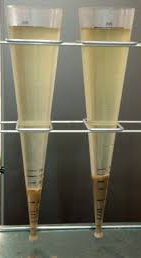
\includegraphics[scale=0.7]{ImhoffCone}\\
			      		Imhoff Cone\\
			      		\textit{Note the ml markings at the bottom of the cone}
			      		
			      		
			      	\end{center}
		      \end{minipage}
%			      \end{minipage}
			      	\item One factor which affects settleability is the conveyance time of the sewage to the treatment plant. 			
			      	\item The settleable component of the suspended solids will decrease as the sewage becomes more septic due to longer conveyance times.
			\item Influent and effluent total suspended solids are measured to establish the overall treatment and individual process efficiencies.  
			\item Volatile solids measurements before and after biological processes such as secondary treatment and digestion provide information on the process efficiency.\\
		\end{itemize}

% 			\end{enumerate}
	\subsection{Summary of Wastewater Solids}\index{Summary of Wastewater Solids}		
% 			\begin{snugshade*}
% 				\item \noindent\textsc{Summary of Wastewater Solids}
% 			\end{snugshade*}
			\begin{itemize}
				\item Solids in wastewater can be categorized as dissolved or suspended
				      \begin{itemize}
				      	\item Suspended solids can be further categorized as settleable or unsettleable
				      \end{itemize}
				\item Solids can also be categorized as organic (aka: volatile) or inorganic (aka: fixed)
				\item Colloidial particles are small sized particles some of which pass through the filter and accounted as part of dissolved solids
				\item TSS - Total Suspended Solids are the solids that are captured on the filter paper upon filtration of the wastewater sample.  
				\item Wastewater samples typically analyzed for TSS include:  plant, primary and secondary processes - influent and effluent.  TSS is reported in mg/l
				\item TS - Total Solids are solids content of sludge.  TS of sludge is established by drying a preweighed quantity of sludge in an oven and is typically reported as \% solids - which is how many parts (by weight) of solids per 100 parts (by weight) of sludge.
				\item Volatile solids are solids that are removed when the solids are incinerated at 550C.  The solids that remain after incineration are fixed or non-volatile or inorganic solids.
			\end{itemize}
	\subsection{Wastewater Solids Content}\index{Wastewater Solids Content}			
% 			\begin{snugshade*}
% 				\item \noindent\textsc{Typical influent wastewater contains:}
% 			\end{snugshade*}
			\begin{itemize}
				\item Less than 0.1\% total solids.  Total solids concentration in typical wastewater is about 750mg/l
				\item The total solids are 50\% organic (volatile) and 50\% inorganic (fixed)
				\item Of the total solids, dissolved solids constitute about 70\% of the solids and the remaining 30\% solids are suspended solids
				\item 40\% of the dissolved solids are volatile the remaining 60\% are fixed
				\item 70\% of the suspended solids are volatile and the remaining 30\% are fixed
			\end{itemize}
			% \clearpage\thispagestyle{empty}
			\begin{figure}[!htbp]
			\vspace{2cm}
				\begin{center}
					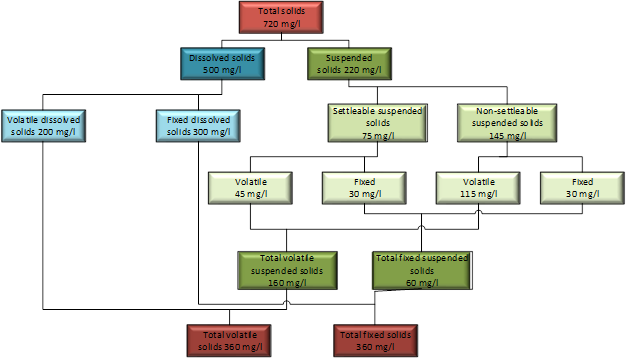
\includegraphics[scale=0.8]{WastewaterSolids}\\
					\caption{Typical Wastewater Solids Concentrations}
				\end{center}
				\end{figure}
% % 			\end{enumerate}
				
\section{Nutrients}\index{Nutrients}	
% 			\begin{snugshade*}
% 				\item \noindent\textsc{Nutrients}
% 			\end{snugshade*}	
			\begin{itemize}
				\item Plant nutrients - nitrogen and phosphorous, present in wastewater effluent discharge, promote growth of plant and algal matter in the receiving waters causing destruction of the normal aquatic life mainly due to oxygen depletion - eutrophication.
				      
				\item Because of the potential impacts of the presence of these nutrients in wastewater effluent on the receiving waters,  limits on the levels of these nutrients is typically stipulated in the treatment plant's wastewater discharge permit.
				      
				\item Typically, conventional secondary treatment processes are designed primarily remove the organics from the wastewater.  Secondary treatment process designed to additionally remove nutrients is deemed as tertiary or advanced treatment is termed as Biological Nutrient Removal (BNR).
			\end{itemize}
	\subsection{Nitrogen}\index{Nitrogen}				
% 			\begin{enumerate}%@@@@@@@@@@@@@@@@@@%
% 				\definecolor{shadecolor}{RGB}{220,220,220}
% 				\begin{snugshade*}
% 					\item \noindent\textsc{Nitrogen}%@@@@@@@@@@@@@@@@@@%
% 				\end{snugshade*}

	\textbf{Forms of nitrogen:}\\	
% 				\begin{itemize}
% 					\item Forms of nitrogen:\\
					      \begin{itemize}
					      	\item About 60\% of nitrogen in wastewater is present as ammonia nitrogen (about 60\%).  The ammonium nitrogen is present either in the form of ammonia (NH$_3$ ) or as ammonium (NH$_4^+$ ) ion.   These two forms can rapidly change from one to the other depending on pH and temperature.  Under low pH (acidic) or neutral conditions – pH less than or equal to 7, ammonia exists mostly as ammonium.  Ammonia becomes the dominant form as the pH increases to 8 and beyond.
					      	\item The other dominant form of nitrogen, about 40\% of the total nitrogen is as organic nitrogen
					      	\item Nitrogen measured as Total Kjeldahl Nitrogen (TKN) which is the sum of the organic nitrogen and the ammonia nitrogen concentrations.  Total inorganic nitrogen is the total concentration of ammonia nitrogen, NO3-, and NO2-.   Table provides the concentrations and forms of nitrogen in wastewater.
					      \end{itemize}
					      \setlength{\arrayrulewidth}{0.7mm}
					      \setlength{\tabcolsep}{8 pt}
					      \renewcommand{\arraystretch}{0.8}
					      \begin{center}
					      \begin{figure}[!htbp]
					      	\noindent \begin{tabular}[!htbp]{ |p{6cm}|p{2.0cm}|p{2.5cm}|p{2.cm}|}
					      	\hline
					      	\multicolumn{4}{|c|}{\textbf{Forms of Nitrogen in Wastewater}} \\
					      	\hline
					      	%\thead{A Head} & \thead{A Second \\ Head} & \thead{A Third \\ Head} \\
					      	%\hline%
					      	
					      	\hspace{1.8 cm}Forms of Nitrogen & \hspace{0.25 cm} Formula & \hspace{.4 cm} Found in & \hspace{.4 cm} Typical \newline \hspace{.2 cm}Concentration\\
					      	\hline
					      	\small Ammonia/Ammonium & \small NH$_3$/NH$_4^{\enspace +}$ &  \small Influent wastewater & 30-50 mg/l\\
					      	
					      	Total Kjeldahl Nitrogen \newline  \small (Ammonia/Ammonium + Organic Nitrogen) &  \small TKN &  \small Wastewater \newline  \small effluent  & 30-60 mg/l \\
					      	
					      	\small Total Inorganic Nitrogen \newline  \small (Ammonia/Ammonium + Nitrite + Nitrate) & \small TIN &  \small  Wastewater \newline  \small effluent  & 1-40 mg/l \\
					      	
					      	\small Nitrate  & $NO_3^{\enspace -}$ &  \small Nitrified effluent &  \small 1-35 mg/l \\
					      	
					      	\small Nitrate  &  $NO_2^{\enspace -}$ &  \small Partially nitrified effluent &  \small 0.1-2 mg/l \\
					      	
					      	\hline
					      	\end{tabular}
					      	\caption{Forms of Nitrogen}
					      	\end{figure}
					      \end{center}
					      
		\subsection{Phosphorous}\index{Phosphorous}			
		\textbf{Forms of phosphorous:}\\
					      \begin{itemize}
					      	\item The principal forms are organically bound phosphorus, polyphosphates, and orthophosphates.
					      	\item Organically bound phosphorus originates from body and food waste and, upon biological decomposition of these solids, is converted to orthophosphates. 
					      	\item Polyphosphates originate from synthetic detergents and are hydrolyzed to orthophosphates. Thus, the principal form of phosphorus in wastewater is assumed to be orthophosphates, although the other forms may exist. Orthophosphates consist of the negative ions PO$_4$$^{3-}$, HPO$_4$$^{2-}$, and H$_2$PO$_4$ $^-$.  These may form chemical combinations with cations (positively charged ions).
					      \end{itemize}

\subsection{Oil and Grease}\index{Oil and Grease}	
			Fats, oil and grease in wastewater originate from homes, food establishments and industries.
			\begin{itemize}
				\item Oil and grease content of wastewater is established in the laboratory by extracting it with a solvent - \textit{n}-hexane.  The concentration of oil and grease is reported in mg/l and typical oil and grease content of wastewater ranges from 80 - 120 mg/l
				\item Presence of excessive oils and grease could potentially impact the secondary treatment process
				\item Oils and grease are removed as floatables in primary treatment and sent with the sludge to the digesters
			\end{itemize}
		



%% \documentclass{article}
% %\usepackage[english]{babel}%
% \usepackage{graphicx}
% \usepackage{tabulary}
% \usepackage{tabularx}
% \usepackage[normalem]{ulem}
% \usepackage{cancel}
% \usepackage{tikz} 
% \usepackage{pdflscape}
% \usepackage{colortbl}
% \usepackage{lastpage}
% \usepackage{multirow}
% \usepackage{enumerate}
% \usepackage[shortlabels]{enumitem}
% \usepackage{color,soul}
% \usepackage{pdflscape}
% \usepackage{hyperref}
% %\usepackage[table]{xcolor}
% \usepackage{rotating}
% \usepackage{amsmath}
% \usepackage{fixltx2e}
% \usepackage{framed}
% \usepackage{mdframed}
% \usepackage[T1]{fontenc}
% \usepackage[utf8]{inputenc}
% \usepackage{textcomp}
% \usepackage{siunitx}
% \usepackage{ifthen}
% \usepackage{fancyhdr}
% \usepackage{gensymb}
% \usepackage{newunicodechar}
% \usepackage[document]{ragged2e}
% \usepackage[margin=1in,top=1.1in,headheight=57pt,headsep=0.1in]
% {geometry}
% \usepackage{ifthen}
% \usepackage{fancyhdr}
% \everymath{\displaystyle}
% \usepackage[document]{ragged2e}
% \usepackage{fancyhdr}
% \everymath{\displaystyle}
% \usepackage{empheq}

% \usepackage[most]{tcolorbox}

% \usepackage{booktabs} % Required for nicer horizontal rules in tables


% \usepackage{enumitem}

% %\usepackage[table,xcdraw]{xcolor}
% \usetikzlibrary{arrows}
% \linespread{2}%controls the spacing between lines. Bigger fractions means crowded lines%
% %\pagestyle{fancy}
% %\usepackage[margin=1 in, top=1in, includefoot]{geometry}
% %\everymath{\displaystyle}
% \linespread{1.3}%controls the spacing between lines. Bigger fractions means crowded lines%
% %\pagestyle{fancy}
% \pagestyle{fancy}
% \setlength{\headheight}{56.2pt}

% \definecolor{myblue}{rgb}{.8, .8, 1}
% \newcommand*\mybluebox[1]{%
% \colorbox{myblue}{\hspace{1em}#1\hspace{1em}}}

% \chead{\ifthenelse{\value{page}=1}{
\includegraphics[scale=0.3]{SCC}\\ \textbf \textbf Wastewater Constituents Analysis \& Laboratory Methods}}
% \rhead{\ifthenelse{\value{page}=1}{}{}}
% \lhead{\ifthenelse{\value{page}=1}{}{Wastewater Constituents Analysis \& Laboratory Methods}}
% \rfoot{\ifthenelse{\value{page}=1}{Module 1: WATR 048 - Spring 2019}{Module 1: WATR 048 - Spring 2019}}

% \lfoot{Shabbir Basrai}
% \cfoot{Page \thepage\ of \pageref{LastPage}}
% \renewcommand{\headrulewidth}{2pt}
% \renewcommand{\footrulewidth}{1pt}
% \begin{document}
% %\begin{empheq}[box=\mybluebox]{align}
% %a&=b\\
% %E&=mc^2 + \int_a^a x\, dx
% %\end{empheq}

% \newlist{steps}{enumerate}{1} % Defines "Steps" for enumerate as Step 1, Step 2 etc.
% \setlist[steps, 1]{label = Step \arabic*:} % Defines "Steps" for enumerate as Step 1, Step 2 etc.

% \setlist{nolistsep} % Reduce spacing between bullet points and numbered lists


%_______________________________________________________________________________________________________________________________________%
\chapterimage{PropertiesandParametersImg.png} % Chapter heading image

\chapter{Wastewater Properties and Parameters}
			
		Laboratory and field tests are conducted to measure parameters which are critical for monitoring and controlling treatment.  The following are the key parameters that are measured.	
			
\subsection{pH}\index{pH}	
			\hl{pH is a measure of the hydrogen ion (H$^+$) content or the acidity or basicity of a solution.}  pH impacts the chemical and micribiological elements of wastewater treatment processes and thus pH measurement and control is critical.
			\begin{itemize}
				\item Pure water dissociates into equal concentration of hydrogen ions and hydroxide ions:\\ 
				      $H_2O \rightarrow H^+ + OH^-$.
				\item The H$^+$ are responsible for acidic properties and the OH$^-$ ions for the basic properties.  
				\item pH is the inverse of H$^+$ concentration; pH increases when the concentration of H$^+$ decreases relative to the concentration of OH-. 
				\item pH scale ranges from 0 – 14. When the concentration of both H$^+$ and OH$^-$ are equal, as in pure water, it is considered neutral and its pH is 7.0.  \item If the pH of a sample solution is below 7.0, the sample is termed acidic and is alkaline or basic if its pH is above 7.0. 
				\item Each change of 1 pH unit represents a 10 fold change in concentration.  For example, a sample with a pH of 2.0 is 1000 times more acidic than a sample with a pH of 5.0. 
				\item pH is measured by an electrode that is sensitive only to H$^+$ or using a pH strip which is essentially an adsorbent paper which is pre-impregnated with chemicals which change color under different H$^+$ concentrations.
				\item Most organisms involved in biological wastewater treatment processes do well within a a narrow range of pH near neutral (pH of 7).			
			\end{itemize}
			
\subsection{Oxidation Reduction Potential (ORP)}\index{Oxidation Reduction Potential (ORP)}			
			\begin{itemize}
				\item ORP measurements are common in wastewater process control for monitoring conditions and process efficiency
				\item ORP is measured in milivolts (mV) using a probe\\
				\item ORP is a measure of the potential of oxidation/reduction – electron transfer, based chemical reactions to occur 
				\item If the measured ORP value (in mV), is positive it indicates an environment where oxidation will occur and if negative, an environment where reduction reactions will occur
				\item Higher positive value indicates a stronger oxidative environment and likewise, a lower (more negative) ORP value indicates a stronger reductive environment 
				\item For example, during chlorine disinfection, which is an oxidation process, the wastewater will exhibit a positive ORP.  Stronger the oxidative power of chlorine, higher will be the wastewater ORP value
				\item All living matter, including microbes depend upon respiration to generate energy and respiration involves series of chemical oxidation-reduction reactions 
				\item Bacteria grow and thrive only in specific chemical - oxidative-reductive environments which support its inbuilt metabolic pathways
				\item Aerobic bacteria need molecular oxygen as the terminal electron acceptor as part of its cellular respiration proces.  Bacteria adapted to exist in an environment where molecular oxygen is not present (anoxic and anaerobic), rely on electron acceptors such as NO$_3^-$ (denitrification), SO$_4^-$ (sulfide formation) and carbon (methane formers in anaerobic digestion)
				\item Aerobic bacteria responsible for cBOD removal in the secondary treatment process would be inhibited or wiped-out if the wastewater oxidation potential dropped and become reductive.  Likewise, if the wastewater in the sewer pipes which is normally of reductive (negative ORP)  was to become oxidative because of aeration (dissolving oxygen) it would cease the hydrogen slufide activity of the anaerobic bacteria
				\end{itemize}
		
			\setlength{\arrayrulewidth}{0.6mm}
			\setlength{\tabcolsep}{8 pt}
			\renewcommand{\arraystretch}{1.2}
			\begin{center}
			\begin{table}[!htbp]
				\begin{tabular}{ |p{9.5cm}|p{4.0cm}|}
					\hline
					\multicolumn{2}{|c|}{\textbf{Typical Wastewater Process ORPs}} \\
					\hline
					
					\hline
					\small Clorine disinfection & \small +650 to +700 mV  \\
					\small Nitrification & \small +100 to +350 mV   \\
					\small Biological phosphorous removal & \small +20 to +250mV        \\
					\small Activated sludge	cBOD degradation with free molecular oxygen & \small +50 to +250 mV  \\
					\small Denitrification                                              & \small +50 to -50 mV   \\
					\small Influent wastewater                                          & \small - 200 mV  \\ 
					\small Sulfide formation                                & \small -50 to -250 mV  \\
					\small Anaerobic Digestion: Acid formation (Acidogenesis)           & \small -100 to -225 mV \\
					\small Biological phosphorous removal & \small -100 to -250 mV \\
					\small Anaerobic Digestion: Methane production  (Methanogenesis)     & \small -75 to -400 mV  \\
					\hline
				\end{tabular}
	\end{table}			
			\end{center}
			
\subsection{Alkalinity}\index{Alkalinity}	
			\begin{itemize}
				\item \hl{Alkalinity is the ability of a water to neutralize acids.}  
				\item During certain wastewater treatment processes including anaerobic digestion, acids are generated as a result of microbiological activity.  The bacteria and other biological entities which play an active role in wastewater treatment are most effective at a neutral to slightly alkaline pH of 7 to 8.  In order to maintain these optimal pH conditions for biological activity there must be sufficient alkalinity present in the wastewater to neutralize acids generated by the active biomass.
				\item This ability to maintain the proper pH in the wastewater as it undergoes treatment is the reason why alkalinity is so important to the wastewater industry.
				\item The alkalinity is due to the presence of acid neutralizing bases in the water including the hydroxyl (OH$^-$), carbonate (CO$_3$$^-$) and bicarbonate (HCO$_3$$^-$)  ions.  These ions are of mineral origin and are also formed from carbon dioxide which comes from the atmosphere and from the microbial decomposition of organic material.  The resistance to pH change of the water will continue until all the alkalinity contributing ions are neutralized.  
				\item The pH of a water serves as a guide to the types of alkalinity present in the water but is unrelated to the alkalinity content of a water.  Important Note:  Alkalinity is a measure of the ability to neutralize acids whereas a solution is termed alkaline (or basic) if its pH greater than 7. 
				\item Alkalinity is expressed as milligrams per liter of CaCO$_3$
			\end{itemize}
			
\subsection{Dissolved Oxygen}\index{Dissolved Oxygen}	
			\begin{itemize}
				\item Dissolved oxygen (DO) is the concentration of oxygen dissolved in the wastewater sample and is typically measured in the field using a DO probe.  A titration based Winkler Test is used in the laboratory
				\item The \hl{presence of oxygen indicates an aerobic environment} where dissolved, free oxygen is available for aerobic microorganisms to live, BOD removal in the activated sludge process occurs as a result of the activity of aerobic bacteria.  The absence of DO indicates that the environment or condition is either anoxic or anaerobic.  
				\item \hl{In an anoxic environment, free oxygen is not present, but oxygen is available from its combined  forms - nitrate (NO$_3$ $^-$) and sulfate (SO$_4$ $^-$)} for the the consumption of microorganisms.  Example of an anoxic process is denitrification.  In denitrification, the anoxic bacteria in the presence of food (cBOD) consume the combined oxygen in nitrates (NO$_3$ $^-$ ) and convert it to nitrogen gas.
				\item \hl{The complete absence of oxygen including free and combined oxygen is an anaerobic environment.}
				\item Microorganisms are termed as obligate aerobes if they cannot survive without free oxygen.  Facultative aerobes are microorganisms which can survive in both aerobic and anaerobic environments.  
			\end{itemize}
			
\subsection{Microbiological testing and monitoring}\index{Microbiological testing and monitoring}	
			
			Microbes play a critical role in wastewater treatment.  
			\begin{itemize}
				\item Heterotrohic (organisms that consume organic material) microbes are responsible for the biological wastewater treatment processes - secondary treatment process, digestion and nutrient removal; and
				\item Pathogens - agents that cause disease are present in wastewater effluent.
			\end{itemize}
Microbiological testing and monitoring is conducted as part of the wastewater treatment typically for the following:
\begin{enumerate}[1.]
				
				\item Microbiological testing related to monitoring and troubleshooting biological wastewater treatment\\
				
				Microbes involved in biological wastewater treatment processes include:\\
				\begin{itemize}
					\item Fungi - Filamentous fungi occasionally bloom in activated sludge processes due to low pH or nutrient deficiency and cause problems with the settleability.
					\item Protozoa - Protozoas play a important role in the secondary treatment process.  Common protozoas in the activated sludge process include:
					      \begin{itemize}
					      	\item Amoeba
					      	\item Flagellate
					      	\item Cilliate
					      \end{itemize}
					\item Rotifers
					\item Nematodes
					\item Bacteria - Bacteria is the predominant microorganism responsible for the biological wastewater water treatment.  
				\end{itemize}
				\begin{itemize}
					\item The effectiveness of the biological wastewater treatment processes is primarily due to the presence of a microbial ecosystem with a right balance of populations of different microbial species.
					\item Methods used for monitoring the microbial composition include direct monitoring using a light microscope to see which and how many of the different microbial species are present - typically used for activated sludge process.
					\item Indirect method includes monitoring other parameters such as pH and alkalinity which are influenced by microbiological activity.
					\item The microbial monitoring ensures process stability and helps identify potential process upset conditions caused by changes to the microbial population due to other external factors - toxicty, organic loading, temperature etc.
				\end{itemize}

\item Microbiological testing related to monitoring and controlling pathogens in treated wastewater effluent\\

	
				Pathogens in wastewater belong to the following groups:
				\begin{itemize}
					\item Bacteria:  Although, bacteria is present in large numbers in feces, pathogenic or bacteria are present only because of an infection and this pathogenic bacteria can potentially spread the infection to other healthy individuals.  Disease spread by pathogenic bacteria include diarrhea, cholera and typhoid among many others.
					      
					\item Viruses: A large number of viruses may infect humans and are present in feces.  These include enteroviruses (including polioviruses), hepatitis A virus, reoviruses and diarrhea-causing viruses (especially rotavirus).
					      
					\item Protozoa:  Many species of protozoa can infect humans and cause diarrhoea and dysentery. Girardia which casues diarrheal illness is an example of a protozoan pathogen
					      
					\item Helminths:  These are parasitic worms that can infect humans and are transmitted to others through its eggs or larval forms
					      
				\end{itemize}
				
				\begin{itemize}
					\item As one of the main reasons for treating wastewater is to protect public health, microbiological/pathogen testing of the wastewater effluent and the surface water impacted by the wastewater discharge is conducted to meet the requirements of a wastewater discharge permit, to monitor the pathogen impact of treated wastewater discharge and assess the level of contamination of a public body of water.
					\item The bacteriological tests involves detection and quantification of one or more of the following bacteria:  total coliforms, fecal coliforms, E. Coli, and Enterococcus.  
					      \begin{itemize}
					      	\item The main reason why these bacteria such as coliforms and enterococcus are used \hl{as it is not practical to detect and quantify all pathogens associated with wastewater.}  
					      	\item These selected bacteria originate from feces and indicate fecal contamination and thus serve as an indicator organisms for pathogens of wastewater origin.  
					      	\item Also, they are abundant, potentially less harmful, and easy to detect.  E. coli has been shown to be a better predictor of the potential for impacts to human health and therefore many newer wastewater discharge permits require E. Coli testing in lieu of fecal coliform testing requirements.
					      \end{itemize}
					\item The microbiological test sample is always collected as a grab in a clean, sterile borosilicate glass or plastic bottle containing sodium thiosulfate. 
					      \begin{itemize}
					      	\item Sodium thiosulfate is added to remove residual chlorine which will kill coliforms during transit. 
					      	\item If the sample is not preserved or maintained under proper conditions until the test is conducted in the laboratory, the test would provide erroneous results.
					      	\item Samples must be refrigerated if they cannot be analyzed within 1 hour of collection and must be handled with care to prevent contamination and adverse conditions such as prolonged exposure to direct sunlight.
					      	\item The maximum holding time for state or federal permit reporting purposes is 6 hours. 
					      \end{itemize} 
					\item As it is not possible to exactly quantify the number of bacteria present, a statistical based - \hl{Most Probable Number (MPN)} approach is utilized.  The methods for wastewater bacteriological tests include:  multiple-tube fermentation technique, membrane filtration and quanti-tray testing. 
				\end{itemize}
			\end{enumerate}

\subsection{Specific Gravity}\index{Specific Gravity}				
			\begin{itemize}
				\item Specific gravity is a term to express the weight of a solution with respect to that of water
				\item Water weighs 1 kg/L or 8.34 lbs/gallon or 62.4 lbs/ft$^3$
				\item A solution with a specific gravity of 1.2 will weigh 1.2 times the same volume of water.  1 L of that solution will weigh ( 1.2 kg )/L  or  ( 1.2*8.34=10lbs )/gallon.
				\item Typically wastewater and the associated unthickened sludge, for all practical purposes is assumed to have a specific gravity of 1 - implying 8.34 lbs/gallon.
				\item Specific gravity is typically used for calculations related to chemicals used in wastewater treatment.
			\end{itemize}

%% \documentclass{article}
% %\usepackage[english]{babel}%
% \usepackage{graphicx}
% \usepackage{tabulary}
% \usepackage{tabularx}
% \usepackage[normalem]{ulem}
% \usepackage{cancel}
% \usepackage{tikz} 
% \usepackage{pdflscape}
% \usepackage{colortbl}
% \usepackage{lastpage}
% \usepackage{multirow}
% \usepackage{enumerate}
% \usepackage[shortlabels]{enumitem}
% \usepackage{color,soul}
% \usepackage{pdflscape}
% \usepackage{hyperref}
% %\usepackage[table]{xcolor}
% \usepackage{rotating}
% \usepackage{amsmath}
% \usepackage{fixltx2e}
% \usepackage{framed}
% \usepackage{mdframed}
% \usepackage[T1]{fontenc}
% \usepackage[utf8]{inputenc}
% \usepackage{textcomp}
% \usepackage{siunitx}
% \usepackage{ifthen}
% \usepackage{fancyhdr}
% \usepackage{gensymb}
% \usepackage{newunicodechar}
% \usepackage[document]{ragged2e}
% \usepackage[margin=1in,top=1.1in,headheight=57pt,headsep=0.1in]
% {geometry}
% \usepackage{ifthen}
% \usepackage{fancyhdr}
% \everymath{\displaystyle}
% \usepackage[document]{ragged2e}
% \usepackage{fancyhdr}
% \everymath{\displaystyle}
% \usepackage{empheq}

% \usepackage[most]{tcolorbox}

% \usepackage{booktabs} % Required for nicer horizontal rules in tables


% \usepackage{enumitem}

% %\usepackage[table,xcdraw]{xcolor}
% \usetikzlibrary{arrows}
% \linespread{2}%controls the spacing between lines. Bigger fractions means crowded lines%
% %\pagestyle{fancy}
% %\usepackage[margin=1 in, top=1in, includefoot]{geometry}
% %\everymath{\displaystyle}
% \linespread{1.3}%controls the spacing between lines. Bigger fractions means crowded lines%
% %\pagestyle{fancy}
% \pagestyle{fancy}
% \setlength{\headheight}{56.2pt}

% \definecolor{myblue}{rgb}{.8, .8, 1}
% \newcommand*\mybluebox[1]{%
% \colorbox{myblue}{\hspace{1em}#1\hspace{1em}}}

% \chead{\ifthenelse{\value{page}=1}{
\includegraphics[scale=0.3]{SCC}\\ \textbf \textbf Wastewater Constituents Analysis \& Laboratory Methods}}
% \rhead{\ifthenelse{\value{page}=1}{}{}}
% \lhead{\ifthenelse{\value{page}=1}{}{Wastewater Constituents Analysis \& Laboratory Methods}}
% \rfoot{\ifthenelse{\value{page}=1}{Module 1: WATR 048 - Spring 2019}{Module 1: WATR 048 - Spring 2019}}

% \lfoot{Shabbir Basrai}
% \cfoot{Page \thepage\ of \pageref{LastPage}}
% \renewcommand{\headrulewidth}{2pt}
% \renewcommand{\footrulewidth}{1pt}
% \begin{document}
% %\begin{empheq}[box=\mybluebox]{align}
% %a&=b\\
% %E&=mc^2 + \int_a^a x\, dx
% %\end{empheq}

% \newlist{steps}{enumerate}{1} % Defines "Steps" for enumerate as Step 1, Step 2 etc.
% \setlist[steps, 1]{label = Step \arabic*:} % Defines "Steps" for enumerate as Step 1, Step 2 etc.

% \setlist{nolistsep} % Reduce spacing between bullet points and numbered lists


%_______________________________________________________________________________________________________________________________________%
\chapterimage{SamplingCoverBW.png}
\chapter{Wastewater Sampling}		
		\begin{itemize}
			\item Field or laboratory measurement of a certain parameter is critical in wastewater treatment operations to obtain information about wastewater characteristics in order to either characterize a wastewater stream, or to monitor a treatment process or for permit compliance.  
			\item A sample is a small part of the whole representing the whole.  Thus, a sample needs to be such that it truly represents the entire population – which in a wastewater operations could be either a wastewater stream, wastewater solids or a chemical used.
		\end{itemize}
		
\section{Sampling Methods}\index{Sampling Methods}
\subsection{Grab Samples}\index{Grab Samples}
				\begin{itemize}
					\item A grab sample is a sample collected at a specific spot at a site over a short period of time.  
					\item Grab sampling allows for instantaneous analysis of parameters such as pH, dissolved oxygen, chlorine residual, temperature and other parameters which change rapidly with time.
					\item A grab sample represents a snapshot of space and time of a process stream.
					\end{itemize}
\subsection{Composite Samples}\index{Composite Samples}
				\begin{itemize}
					\item A composite sample is a collection of discrete samples are combined over a certain period or space and therefore represent the average performance of a wastewater treatment plant or a process during the collection period.\\  
					\item Composite sampling can be either based on:
					      
					      1. constant time interval (time proportioned sampling)\\
					      2. constant wastewater volume interval (flow-proportioned sampling), and\\
					      3. treatment process space - includes samples taken at different depths\\
					      
					\item Composite samples are typically collected using automated samplers which can be programmed to collect samples at pre-established time intervals – for time proportional sampling.
					\item Time and space composite samples are collected by adding equal volumes of samples collected from different times or locations.  
					\item Flow proportional composite samples comprise of volume of each subsample based on flow.\\  
				\end{itemize}
				
			\begin{center}
				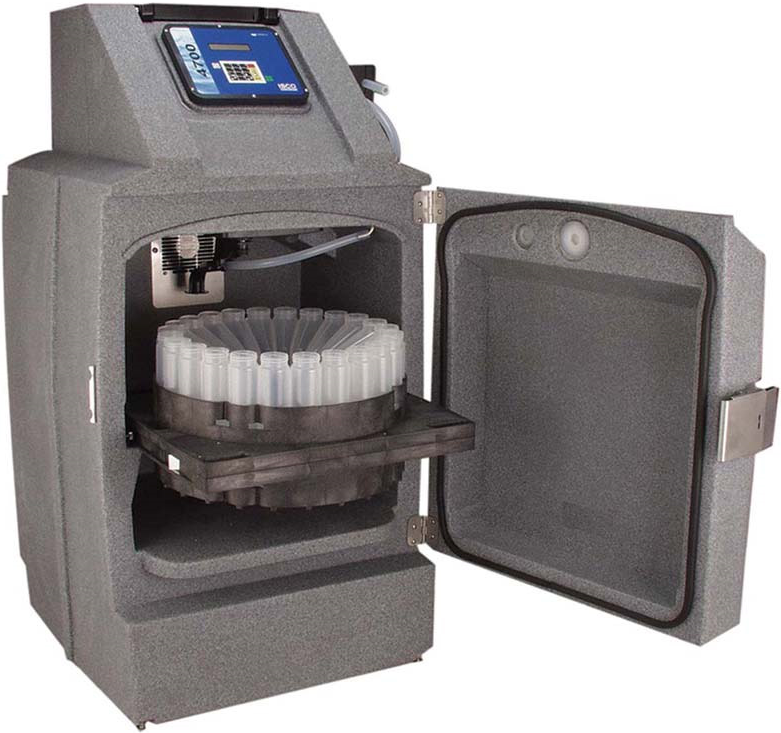
\includegraphics[scale=0.2]{Autosampler} \hspace{2cm} 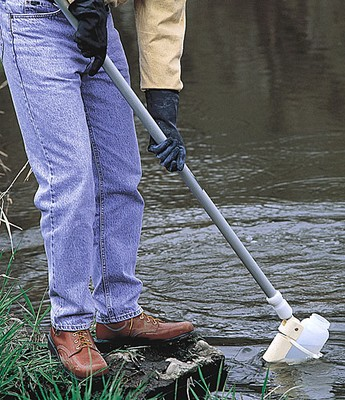
\includegraphics[scale=0.37]{Grabsampler}\\
			\end{center}
			\hspace{2.3cm} Automated Sampler \hspace{2.0cm} \parbox{\textwidth}{Grab Sampling Using a Long Handle Dipper}\\

\subsection{Sampling Precautions and Protocols}\index{Sampling Precautions and Protocols}
			\begin{itemize}
				\item Samples should represent the major portion of the process or the process stream and should be taken from places where the mixing is thorough, avoiding dead spots and areas of heavier or lighter loadings. 
				\item The collected sample is invariably exposed to conditions very different from the original source and is subject to change due to chemical and microbiological activity.  
				\item Thus, in order to ensure integrity of sample, sample preservation techniques specific to the analysis to be performed is needed.  
				      \begin{itemize}
				      	\item The preservation technique should not only allow for stabilizing the parameter to be analyzed, it should also not interfere with the analyses.  
				      	\item The common preservation techniques involve use of proper containers, temperature control, addition of chemical preservatives, and observance of the recommended maximum sample holding time.
				      \end{itemize}
			\end{itemize}
			
\subsection{Bacteriological Sampling}\index{Bacteriological Sampling}
\begin{itemize}
\item Always collected as a grab
\item A clean, sterile borosilicate glass or plastic bottle containing sodium thiosulfate is used. Sodium thiosulfate is added to remove residual chlorine which will kill coliforms during transit. If the sample is not preserved or maintained under proper conditions until the test is conducted in the laboratory, the test would provide erroneous results
\item Samples must be refrigerated if they cannot be analyzed within 1 hour of collection
\item Samples must be handled with care to prevent contamination and adverse conditions such as prolonged exposure to direct sunlight
\item Maximum holding time for state or federal permit reporting purposes is 6 hours
\end{itemize} 

\section{Data Reporting}\index{Data Reporting}	
		\begin{itemize}
			\item Arithmetic mean is typically calculated for reporting data where multiple samples have been collected and analyzed for the same process stream at different times and for reporting average value over a certain time period – daily, monthly etc.\\ \item Arithmetic mean mathematically is calculated by adding all the result values and dividing by the total number of data points.\\
		\end{itemize}
		Mathematically the arithmetic mean is represented as:\\
		$$\bar{x}=\frac{\sum_{i=1}^{n} x^i}{n} = \frac{x_1+x_2+x_3...x_n}{n}$$
		For example:\\
		Arithmetic mean of the following set of data points:  200, 304, 250, 400 is calculated as:\\
		\vspace{10pt}
		Arithmetic Mean = $\frac{200 + 302 + 250 + 400}{4}= 288$\\
		\vspace{10pt}
		For data sets for analysis such as fecal coliform could include values which vary by several orders of magnitudes, using the arithmetic mean to report the average value is not appropriate as the lower or higher values would bias the calculated mean.\\
		\vspace{10pt}
		For example, consider a data set with values:  260, 300, 500, 5,000, 320 and 200.\\
		\vspace{10pt}
		The arithmetic mean = $\frac{260+300+500+5,000+320+200}{6} = 3,444$\\
		Here the 5000 value completely skews the arithmetic mean.
		
		Therefore, for such tests, the geometric mean calculation is used for reporting the average value.\\
		
		
		Mathematically a geometric mean is represented as:\\
		$$\Bigg(\prod_{i=a}^n\Bigg)^{\frac{1}{n}}=\sqrt[n]{a_1*a_2*a_3...a_n}$$
		 
		Calculation method:\\
		1.	Find the product of all the data points (analogous to first calculating the sum of all the data points when calculating the arithmetic mean)\\
		260*300*500*5,000*320*200 = 12,480,000,000,000,000\\
		2.	Raise the product to the inverse of the number of data points\\
		(*Using the power function of a scientific calculator)\\
		Here n (\# data points) = 6 $\implies$ geometric mean = $(12,480,000,000,000,000)^{\frac{1}{6}}   = 482$



%\chapterimage{ChapterImageLaboratory.png} % Chapter heading image

\chapter{Laboratory Analysis}

% \section{Paragraphs of Text}\index{Paragraphs of Text}


% \everymath{\displaystyle}
% \linespread{2}%controls the spacing between lines. Bigger fractions means crowded lines%
% %\pagestyle{fancy}
% %\usepackage[margin=1 in, top=1in, includefoot]{geometry}
% %\everymath{\displaystyle}
% \linespread{2}%controls the spacing between lines. Bigger fractions means crowded lines%
% %\pagestyle{fancy}
% \pagestyle{fancy}
% \setlength{\headheight}{56.2pt}
% \colorlet{Mycolor1}{green!10!orange!90!}

% \chead{\ifthenelse{\value{page}=1}{
\includegraphics[scale=0.3]{SCC}\\ \textbf \textbf Introduction to Wastewater Treatment}}
% \rhead{\ifthenelse{\value{page}=1}{}{}}
% \lhead{\ifthenelse{\value{page}=1}{}{\textbf Introduction to Wastewater Treatment}}
% \rfoot{\ifthenelse{\value{page}=1}{Module 1: WATR 048 - Spring 2019}{Module 1: WATR 048 - Spring 2019}}

% \cfoot{Page \thepage\ of \pageref{LastPage}}
% \lfoot{Shabbir Basrai}
% \renewcommand{\headrulewidth}{2pt}
% \renewcommand{\footrulewidth}{1pt}

% \newcommand{\stkout}[1]{\ifmmode\text{\sout{\ensuremath{#1}}}\else\sout{#1}\fi}
% %Defining colour with different models.
% \definecolor{mypink1}{rgb}{0.858, 0.188, 0.478}
% \definecolor{mypink2}{RGB}{219, 48, 122}
% \definecolor{mypink3}{cmyk}{0, 0.7808, 0.4429, 0.1412}
% \definecolor{mygray}{gray}{0.6}
% \colorlet{LightRubineRed}{RubineRed!70!}
% \colorlet{Mycolor1}{green!10!orange!90!}
% \definecolor{Mycolor2}{HTML}{00F9DE}

% %New command used in the table with all available colour names
% \newcommand{\thiscolor}[1]{\texttt{#1} \hfill \fcolorbox{black}{#1}{\hspace{2mm}}}

% %This changes the row separation in the table
% \renewcommand{\arraystretch}{1.5}




%\noindent\textsc{Area \& Volume Math Problems}
%\definecolor{shadecolor}{RGB}{200,200,240}
% \item \noindent\textsc{Why Treat Wastewater}


		\section{BOD Analysis}\index{BOD Analysis}		
\begin{itemize}
\setlength\itemsep{1em}

\item The Biochemical Oxygen Demand (BOD) test estimates the amount of biodegradable material present by measuring the amount of oxygen used by the bacteria to break down the organic waste in the sample incubated at 20 deg. C over a five-day period . The BOD test provides an indication on the strength of wastewater in terms of how much oxygen could be depleted if that wastewater was introduced into another receiving water.  Complete stabilization of a sample may require a period of incubation too long for practical purposes; therefore, 5 days has been accepted as the standard incubation period.

\item As the regular BOD test includes estimation of oxygen nitrifying bacteria consumes in the process of converting inorganic forms of ammonia and nitrogen to nitrite and nitrate, its value represents oxygen used for removing both, organic material and nitrogenous matter.  As this BOD value does not quite represent the organic strength of the wastewater, the normal BOD test is modified by introducing a chemical inhibitor - 3 mg of 2-chloro-6-(trichloro methyl) pyridine (TCMP), which suppresses the growth of the nitrogenous bacteria so that the resultant BOD measured represents the oxygen depletion associated with the depletion of the organic matter only.  This is the Carbonaceous biochemical oxygen demand or cBOD. \\
\vspace{0.4cm}
\textbf{Thus tBOD = nBOD + cBOD}

\item Wastewater BOD measurement involves testing a sample set consisting of several sample dilutions along with a "Blank".  "Blank" is a sample with only the dilution water with no wastewater added. \\


\item The dilutions are made based upon the expected BOD concentration of the sample.  Using the final dilution volume of 300 ml, the initial sample volume can be estimated using the formula:\\

\textbf{$Sample \enspace Volume (ml) = \dfrac{\Big[Oxygen \enspace Depletion \Big(\dfrac{mg}{l}\Big)\Big]}{Anticipated \enspace BOD \Big(\dfrac{mg}{l}\Big)}*300 \enspace ml$}\\

\item For example, if testing an influent wastewater BOD with an expected BOD value of 250 mg/l, a range of sample volumes for dilution around sample volume of $\dfrac{4\dfrac{mg}{l}}{250 \dfrac{mg}{l}}*300 \enspace ml$=5ml.\\
\vspace{0.4cm}
\item The data obtained for each of the dilutions after the 5-day incubation period must meet the following criteria for the sample value to be acceptable for calculating the BOD.\\
\vspace{0.4cm}

\begin{enumerate}[1.]
\setlength\itemsep{1em}

\item A residual DO of at least 1 mg/L,
\item A DO depletion of at least 2 mg/L
\end{enumerate}
\vspace{0.4cm}
\item Additionally, the whole sample set is rejected if the Blank shows an oxygen depletion of >0.2mg/l.\\
\vspace{0.4cm}
\item BOD is calculated for each sample dilution value using the following formula:\\
\vspace{0.4cm}
\textbf{$BOD \Big(\dfrac{mg}{l}\Big) = \dfrac{Initial \enspace DO - DO \enspace Day \enspace 5}{Sample \enspace Volume \enspace (ml)}*300 \enspace ml$}\\



\end{itemize}
\vspace{0.4cm}
\section{Wastewater solids}\index{Wastewater solids}

	\subsection{Total (TSS) and Volatile (VSS)}\index{Total (TSS) and Volatile (VSS)}
\begin{itemize}
\setlength\itemsep{1em}
					\item A known volume of wastewater sample is filtered through a pre-weighed filter paper
					\item The suspended solids will be retained by the filter
					\item The water with the dissolved solids will pass through the filter
					\item The filter paper with the filter solids is rinsed with distilled water to remove 
					\item The filter paper with the solids is dried in the oven and then weighed
					\item The difference between the weight of the dried filter paper with the solids and the pre-weighed filter paper, measured in mg, will be the suspended solids in: mg per the original quantity of wastewater sample taken.  This value can be converted to give the suspended solids content in mg/l
					\item A filter paper with the dried solids is incinerated in a muffler furnace
					\item The difference in the weight of the solids, before and after incineration is the fixed solids
					\item The difference between the weight of the solids before incineration and the fixed solids is the volatile solids
	\end{itemize}				

\textbf{Total Suspended Solids - TSS}
\vspace{0.4cm}
$TSS \dfrac{mg}{l}=\dfrac{weight \enspace of \enspace solids \enspace \cancel{gms}}{volume \enspace of \enspace sample \enspace \enspace \cancel{ml}}*\dfrac{1000 \enspace \cancel{ml}}{l}*\dfrac{1000 \enspace mg}{\cancel{gms}}$\\
\vspace{0.3cm}
\hspace{1.4cm}$=\dfrac{weight \enspace of \enspace filter \enspace paper  \enspace with \enspace dried  \enspace solids - weight \enspace of \enspace filter \enspace paper}{volume \enspace of \enspace sample \enspace \enspace (ml)}*1,000,000$\\
\vspace{0.4cm}

\vspace{0.4cm}
\textbf{Volatile Suspended Solids - VSS}	
\vspace{0.4cm}

$VSS \dfrac{mg}{l}=\dfrac{weight \enspace of \enspace volatile \enspace solids \enspace \cancel{gms}}{volume \enspace of \enspace sample \enspace \enspace \cancel{ml}}*\dfrac{1000 \enspace \cancel{ml}}{l}*\dfrac{1000 \enspace mg}{\cancel{gms}}$\\
\vspace{0.3cm}
\hspace{1.4cm}$=\dfrac{wt. \enspace of \enspace filter \enspace paper  \enspace with \enspace dried  \enspace solids - wt. \enspace of \enspace filter \enspace paper \enspace incinerated \enspace residue}{volume \enspace of \enspace sample \enspace \enspace (ml)}*1,000,000$\\
\vspace{0.3cm}
$VSS(\%)=\dfrac{weight \enspace (gms) \enspace of \enspace volatile \enspace solids}{100 \enspace gms \enspace total \enspace solids}=\dfrac{gms \enspace volatile \enspace solids}{\cancel{gms \enspace total \enspace solids}}*\dfrac{100 \cancel{\enspace gms \enspace total \enspace solids}}{100 \enspace gms \enspace total \enspace solids}$\\
\vspace{0.3cm}
\hspace{1.5cm}\small{$=\dfrac{wt. \enspace of \enspace filter \enspace paper  \enspace with \enspace dried  \enspace solids - wt. \enspace of \enspace filter \enspace paper \enspace incinerated \enspace residue}{wt. \enspace of \enspace filter \enspace paper  \enspace with \enspace dried  \enspace solids - wt. \enspace of \enspace filter \enspace paper}*100$}\\				

	\subsection{Wastewater and Sludge Total \& Volatile Solids}\index{Wastewater and Sludge Total \& Volatile Solids}
\vspace{0.4cm}
\begin{itemize}
\setlength\itemsep{1em}
					\item A certain quantity of wastewater (by volume) or sludge (by weight) is taken in a pre-weighed dish and weighed.  \hl{Note:  the sample is not filtered.}
					\item The dish with the sample is dried in an oven
					\item The difference in the weight of the pre-weighed dish from that of the dish with the dried sample is the total solids
					\item The dried solids are incinerated in a muffler furnace
					\item The difference in the weight of the solids, before and after incineration is the fixed solids
					\item The difference between the fixed solids and the total solids is the volatile solids
					\item Total solids of a sludge sample is reported as a \% of the sludge weight.  A 7\% sludge has 7 lbs of solids for every 100 lbs of sludge.
				\end{itemize}
				
				\hl{For sludge samples, volatile solids is typically reported as the volatile solids fraction in \% of the total solids content of the sludge.  For example, if a 8\% sludge (i.e sludge which has 8\% TS or 80,000mg/l solids), is reported to have 70\% volatile, it means that 70\% of the total solids - 0.7*8\%=5.6\% or 56,000mg/l is the sludge volatile solids content.  \emph{70\% volatile does not meet the sludge has 700,000mg/l volatile solids}}\\	

\vspace{0.4cm}
\textbf{Total Solids - TS}			
\vspace{0.4cm}
$TS(\%)=\dfrac{weight \enspace of \enspace solids \enspace (gms)}{100 \enspace gms \enspace of \enspace sample}=\dfrac{gms \enspace solids}{gms \enspace sample}*100$\\
\vspace{0.3cm}
\hspace{1.2cm}$=\dfrac{weight \enspace of \enspace cruicible \enspace with \enspace dried  \enspace solids - weight \enspace of cruicible}{weight \enspace of \enspace cruicible \enspace with \enspace sample - weight \enspace of cruicible}*100$\\
\vspace{0.4cm}
\textbf{Total Volatile Solids - VS}		
\vspace{0.4cm}
$VS(\%)=\dfrac{weight \enspace of \enspace volatile \enspace solids \enspace (gms)}{100 \enspace gms \enspace of \enspace total \enspace solids}=\dfrac{gms \enspace volatile \enspace solids}{gms \enspace total \enspace solids}*100$\\
\vspace{0.3cm}
\hspace{1.2cm}$=\dfrac{wt. \enspace of \enspace cruicible  \enspace with \enspace dried  \enspace solids - wt. \enspace of \enspace cruicible \enspace incinerated \enspace residue}{wt. \enspace of \enspace cruicible  \enspace with \enspace dried  \enspace solids - wt. \enspace of \enspace cruicible}*100$\\

\newpage
\thispagestyle{empty}
% \begin{landscape}
% \begin{center}
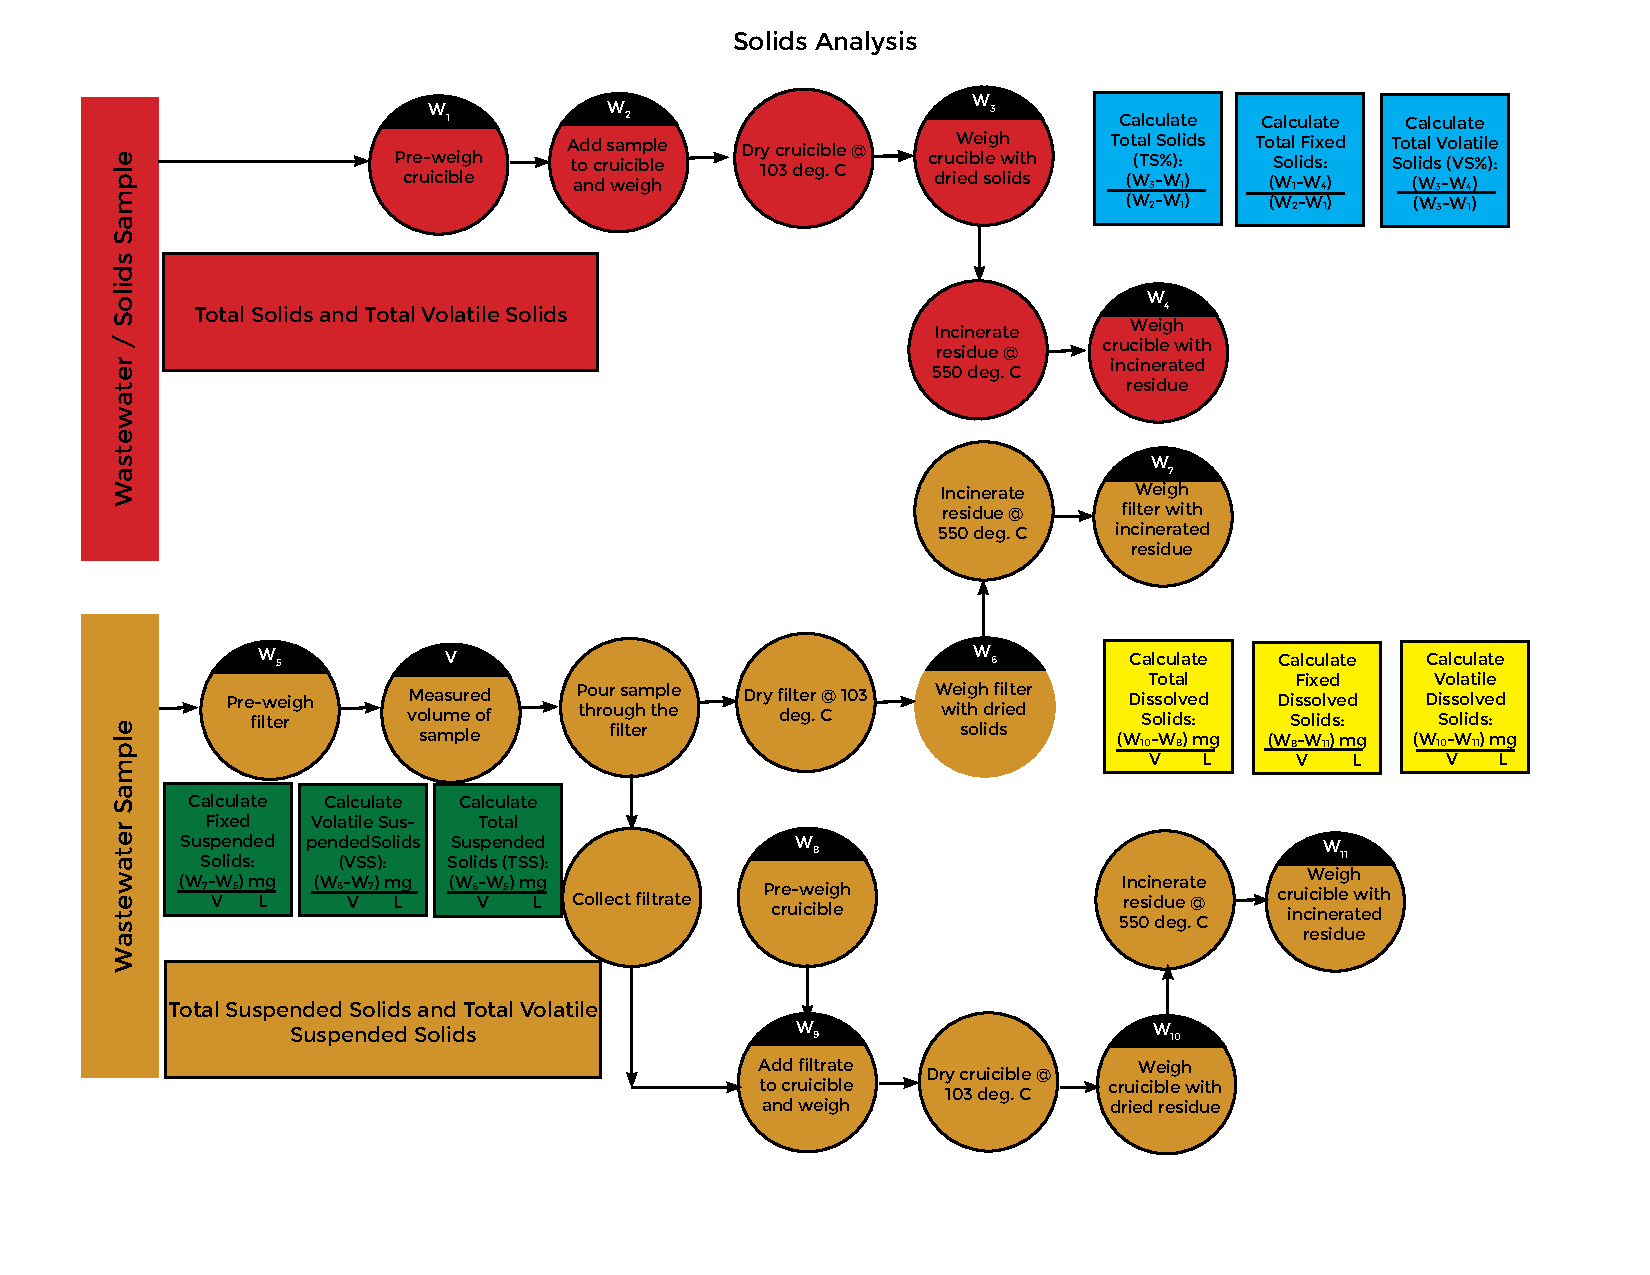
\includepdf[landscape=true]{LaboratorySolidsAnalysis4_01.pdf}
				\newpage
				\thispagestyle{empty}
				\begin{sidewaysfigure}
					\begin{center}
						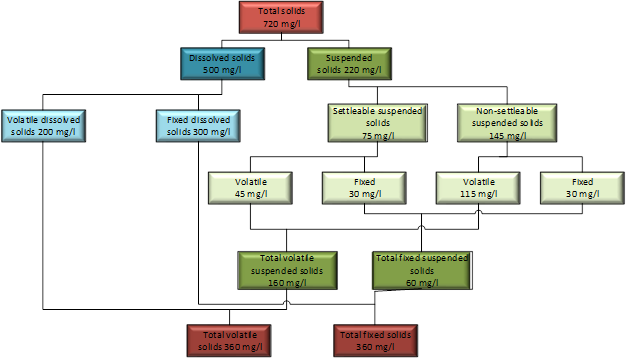
\includegraphics[scale=1.0]{WastewaterSolids}\\
						\caption{Typical Wastewater Solids Concentrations}
					\end{center}
				\end{sidewaysfigure}
%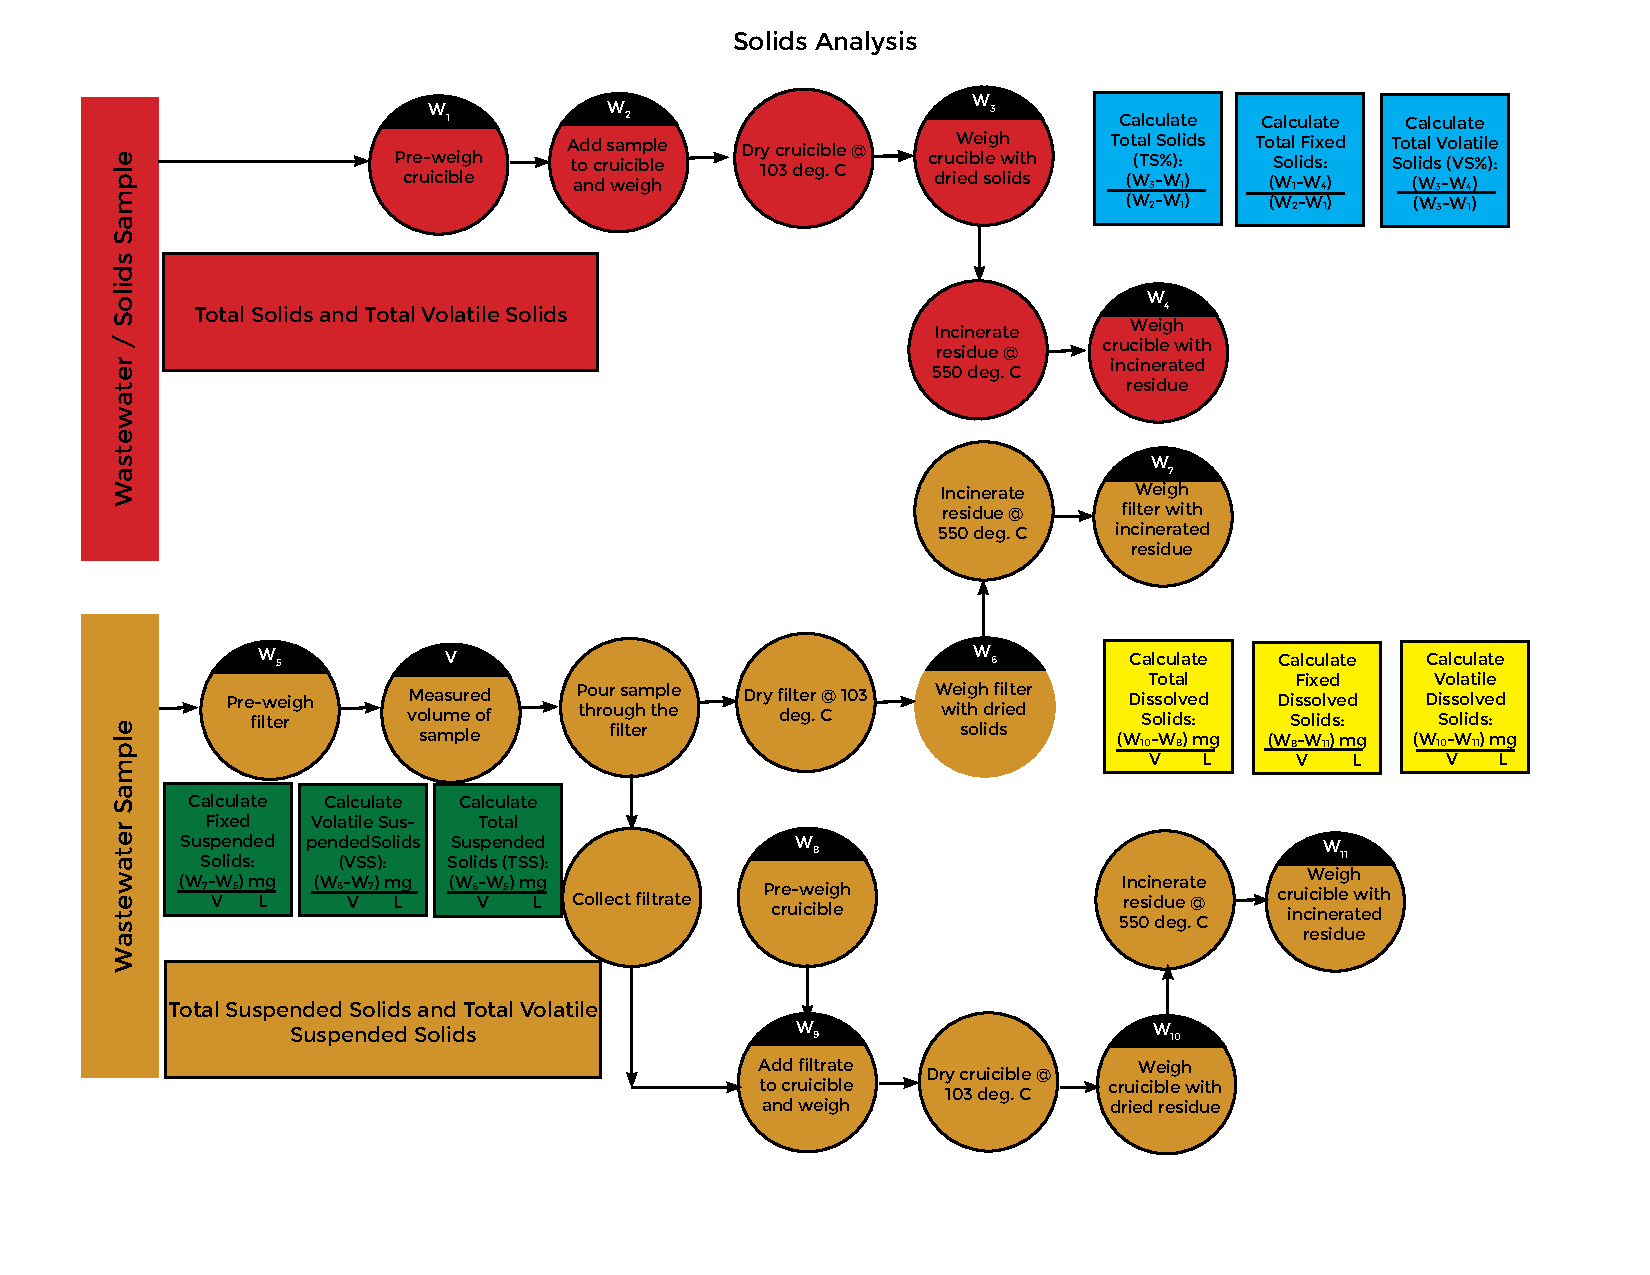
\includegraphics[scale=0.69]{LaboratorySolidsAnalysis4_01.pdf}
% \end{center}
% \end{landscape}
\subsection{Sample BOD and solids analysis math problems}\index{Sample BOD and solids analysis math problems}
\begin{enumerate}
\item BOD tests are run on the final effluent from an activated sludge plant with and without the use of a "nitrification inhibitor". Three hundred milliliter bottles (300 ml) are used in these tests. The raw data for these tests are presented below.  What \textbf{percentage of the average total BOD is the average nBOD}?\\
\vspace{0.5cm}
\begin{tabular}{m {4 cm} m {1.5 cm} m  {1.5 cm} m  {1.5 cm} m  {1.5 cm} m {1.5 cm}}
\cline{1-6}
Sample Volume, ml    & 10 & 20 & 30 & 40 & Blank\\
\hline
Initial DO, mg/l 			& 9.0 	& 	8.9 & 8.8  & 9.1 & 9.1\\
Final DO, mg/l 			& 6.9 	& 	4.8 & 2.5 & 1.1 & 9.0
\end{tabular}
\vspace{0.7cm}\\
BOD Test with "inhibitor" added	(cBOD)\\
\vspace{0.5cm}
\begin{tabular}{m {4 cm} m {1.5 cm} m  {1.5 cm} m  {1.5 cm} m  {1.5 cm} m {1.5 cm}}
\cline{1-6}
Sample Volume, ml    & 10 & 20 & 30 & 40 & Blank\\
\hline
Initial DO, mg/l 			& 8.9 	& 	8.9 & 9.0  & 9.0 & 9.1\\
Final DO, mg/l 			& 7.5 	& 	6.2 & 5.0 & 3.3 & 9.0
\end{tabular}
\vspace{0.5cm}\\
Solution:\\
Blanks for both tBOD and cBOD are both <=0.2mg/l - thus sample sets are acceptable\\
\vspace{0.5cm}
\begin{tabular}{m {3 cm} m {2.5 cm} m  {2.5 cm} m  {2.5 cm} m  {2.5 cm} }
\cline{1-5}
Sample Volume, ml    & 10 & 20 & 30 & 40 \\
\hline
tBOD Diff., mg/l    & 2.1 & 4.1 & 6.3 & 8 \\
tBOD, mg/l    & 2.1*300/10 & 4.1*300/20 & 6.3*300/30 & 8.0*300/40\\
    & =63.0 & = 61.5  & = 63.0 & = 60.0 \\
\hline
cBOD Diff., mg/l    & 1.4 & 2.7 & 4.0 & 5.7 \\
cBOD, mg/l    & Reject & 2.7*300/20 & 4.0*300/30 & 5.7*300/40\\
    & Depletion < 2 & = 40.5  & = 40 & = 42.75 \\
\end{tabular}
\vspace{0.5cm}\\

$tBOD (avg) = (63+61.5+63+60)/4=61.9 \hspace{1cm} cBOD (avg) = (40.5+40+42.75)/3=41.1$\\
nBOD = tBOD - cBOD $\implies$ nBOD = 61.9-41.1=20.8 $\implies$ nBOD(\%)=20.8/61.9*100=$\boxed{33.6\%}$
\vspace{0.5cm}
\item Calculate percent total solids and percent volatile solids of a sludge sample given the following data:\\
\begin{tabular}{m {5 cm} m {0.5 cm} m  {3.5 cm}}
Weight of dish &=&  104.55 gms\\
Weight of dish and wet sludge &= & 199.95 gms\\
Weight of dish and dry sludge &= & 108.34 gms\\
Weight of dish and ash &= & 106.37 gms
\end{tabular}\\
\vspace{0.2cm}
Solution:\\
\vspace{0.2cm}
Weight of dish=104.55 gms\\
Weight of dish and wet sludge=199.95 gms\\
Weight of dish and ash = 106.37 gms\\
\vspace{0.2cm}
$ \implies Weight \enspace of \enspace sludge=199.95-104.55=95.40 \enspace gms$\\
$\implies Weight \enspace of \enspace dry \enspace sludge \enspace (solids)=108.34-104.55=3.79 \enspace gms$\\
$\implies Weight \enspace of \enspace volatile \enspace solids=108.34-106.37=1.97 \enspace gms$\\
\vspace{0.2cm}
$Total \enspace solids (TS\%)=\dfrac{gms \enspace solids}{100 \enspace gms \enspace sludge}=\dfrac{3.79}{95.40} \enspace \dfrac{gms \enspace solids}{\cancel{gms \enspace sludge}}*\dfrac{100 \cancel{\enspace gms \enspace sludge}}{100 \enspace gms \enspace sludge}=\boxed{3.97\%}$\\
\vspace{0.2cm}
$Total \enspace volatile \enspace solids (VS\%) =\dfrac{1.97}{3.79} \enspace \dfrac{gms \enspace volatile \enspace solids}{\cancel{gms \enspace total \enspace solids}}*\dfrac{100 \cancel{\enspace gms \enspace total \enspace solids}}{100 \enspace gms \enspace total \enspace solids}=\boxed{52.0\%}$\\


\end{enumerate}

\section{Bacteriological Ennumeration}\index{Bacteriological Ennumeration}

\begin{tabular}{|c||l|}
\hline
\multicolumn{1}{|c|}{Pathogen} & \multicolumn{1}{c|}{Disease Caused} \\
\hline
Bacteria: &  \\
\hline\hline
Anthrax & anthrax \\
\hline\hline
Escherichia coli & E. coli infection \\
\hline\hline
Myobacterium & tuberculosis \\
tuberculosis &  \\
\hline\hline
Salmonella & salmonellosis, \\
paratyphoid &  \\
\hline\hline
Vibrio cholerae & cholera \\
\hline\hline
Viruses: &  \\
\hline\hline
Hepatitis Virus & Hepatitis A \\
\hline\hline
Polio Virus & polio \\
\hline\hline
Parasites: &  \\
\hline\hline
Cryptosporidium & cryptosporidiosis \\
\hline\hline
Giardia lamblia & giardiasis \\
\hline\hline
\end{tabular}

\begin{itemize}
	\item Involves bacteriological testing of the wastewater effluent and the surface water impacted by the wastewater discharge
	
	\item Conducted in-order to:
		\begin{enumerate}
			\item Meet the requirements of a wastewater discharge permit
			\item Monitor the pathogen impact of treated wastewater discharge
			\item Assess the level of contamination of a public body of water
			\item Bacteriological tests involves detection and quantification of one or more of the following bacteria:  total coliforms, fecal coliforms, \textit{E. Coli}, and \textit{Enterococci}. 
\begin{center}
\tcbox{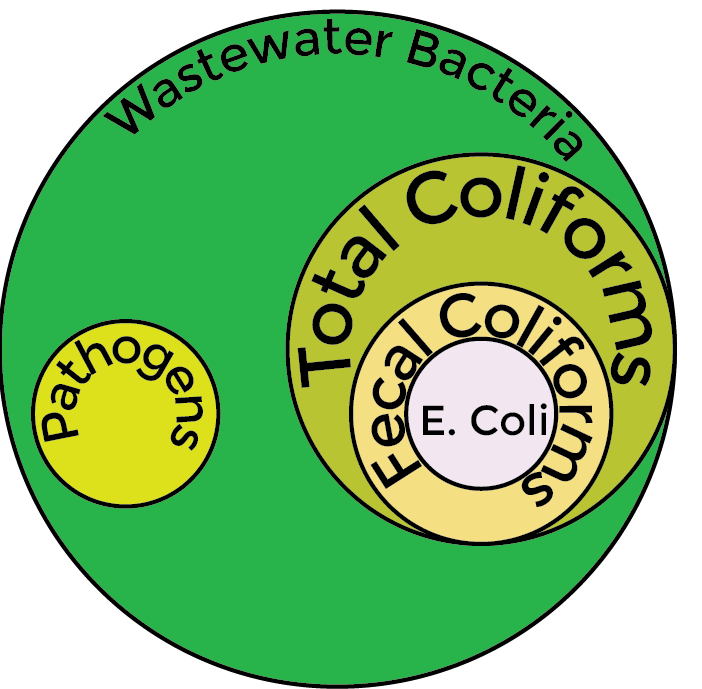
\includegraphics[width=4cm]{LaboratoryWastewaterBacteria}}
Wastewater Bacteria
\end{center}
	
	\item  In wastewater, fecal coliforms originate in the intestines of warm-blooded animals.  Aerobic bacteria including coliforms partake in the metabolization of the organic matter as part of the secondary treatment process
\item Fecal coliforms are seldom pathogenic under normal circumstances and are easily cultured, their presence indicates the potential presence of pathogens

The reason why these bacteria such as coliforms and enterococcus are used:
		\begin{enumerate}
			\item It is not practical to detect and quantify all pathogens associated with wastewater
			\item These bacteria originate from feces and indicate fecal contamination and thus serve as an indicator organisms for pathogens of wastewater origin
			\item They are also:
				\begin{itemize}
					\item abundant
					\item potentially less harmful, and
					\item easy to detect
				\end{itemize}
			\item \textit{E. coli} has been shown to be a better predictor of the potential for impacts to human health and therefore many newer wastewater discharge permits require \textit{E. Coli} testing in lieu of fecal coliform testing requirements.
		\end{enumerate}
		\end{enumerate}

\end{itemize}
 

\subsection{Bacteriological Testing Methods}\index{Bacteriological Testing Methods}
The methods for wastewater bacteriological tests include:  multiple-tube fermentation (MTF) technique, membrane filtration (MF) and quanti-tray testing.  When using the MTF and MF methods, it is not possible to exactly quantify the number of bacteria present, a statistical based - Most Probable Number (MPN) approach is utilized\\
\subsection{The Multiple-Tube Fermentation (MTF) technique}\index{The Multiple-Tube Fermentation (MTF) technique}
This involves adding three volumes – 10 ml, 1 ml and 0.1 ml of the sample, each to a set of five tubes containing Lauryl Tryptose broth and an inverted tube (Durham tube), followed by incubating the tubes at  for a specified time.  The Lauryl Tryptose broth produces color and/or turbidity change due to the growth of the target bacteria and the inverted tube collects the gas produced by the bacterial respiration.  At the end of the process, the number of tubes showing bacterial growth are counted for each volume of sample and using this information the concentrations of organisms in the original sample are established using Statistical Tables.  The test is conducted in three parts – presumptive, confirmative and completed.  A schematic of the MTF used for quantifying total coliforms and fecal coliforms is provided below.\\
\newpage
\thispagestyle{empty}
% \begin{landscape}
% \begin{center}
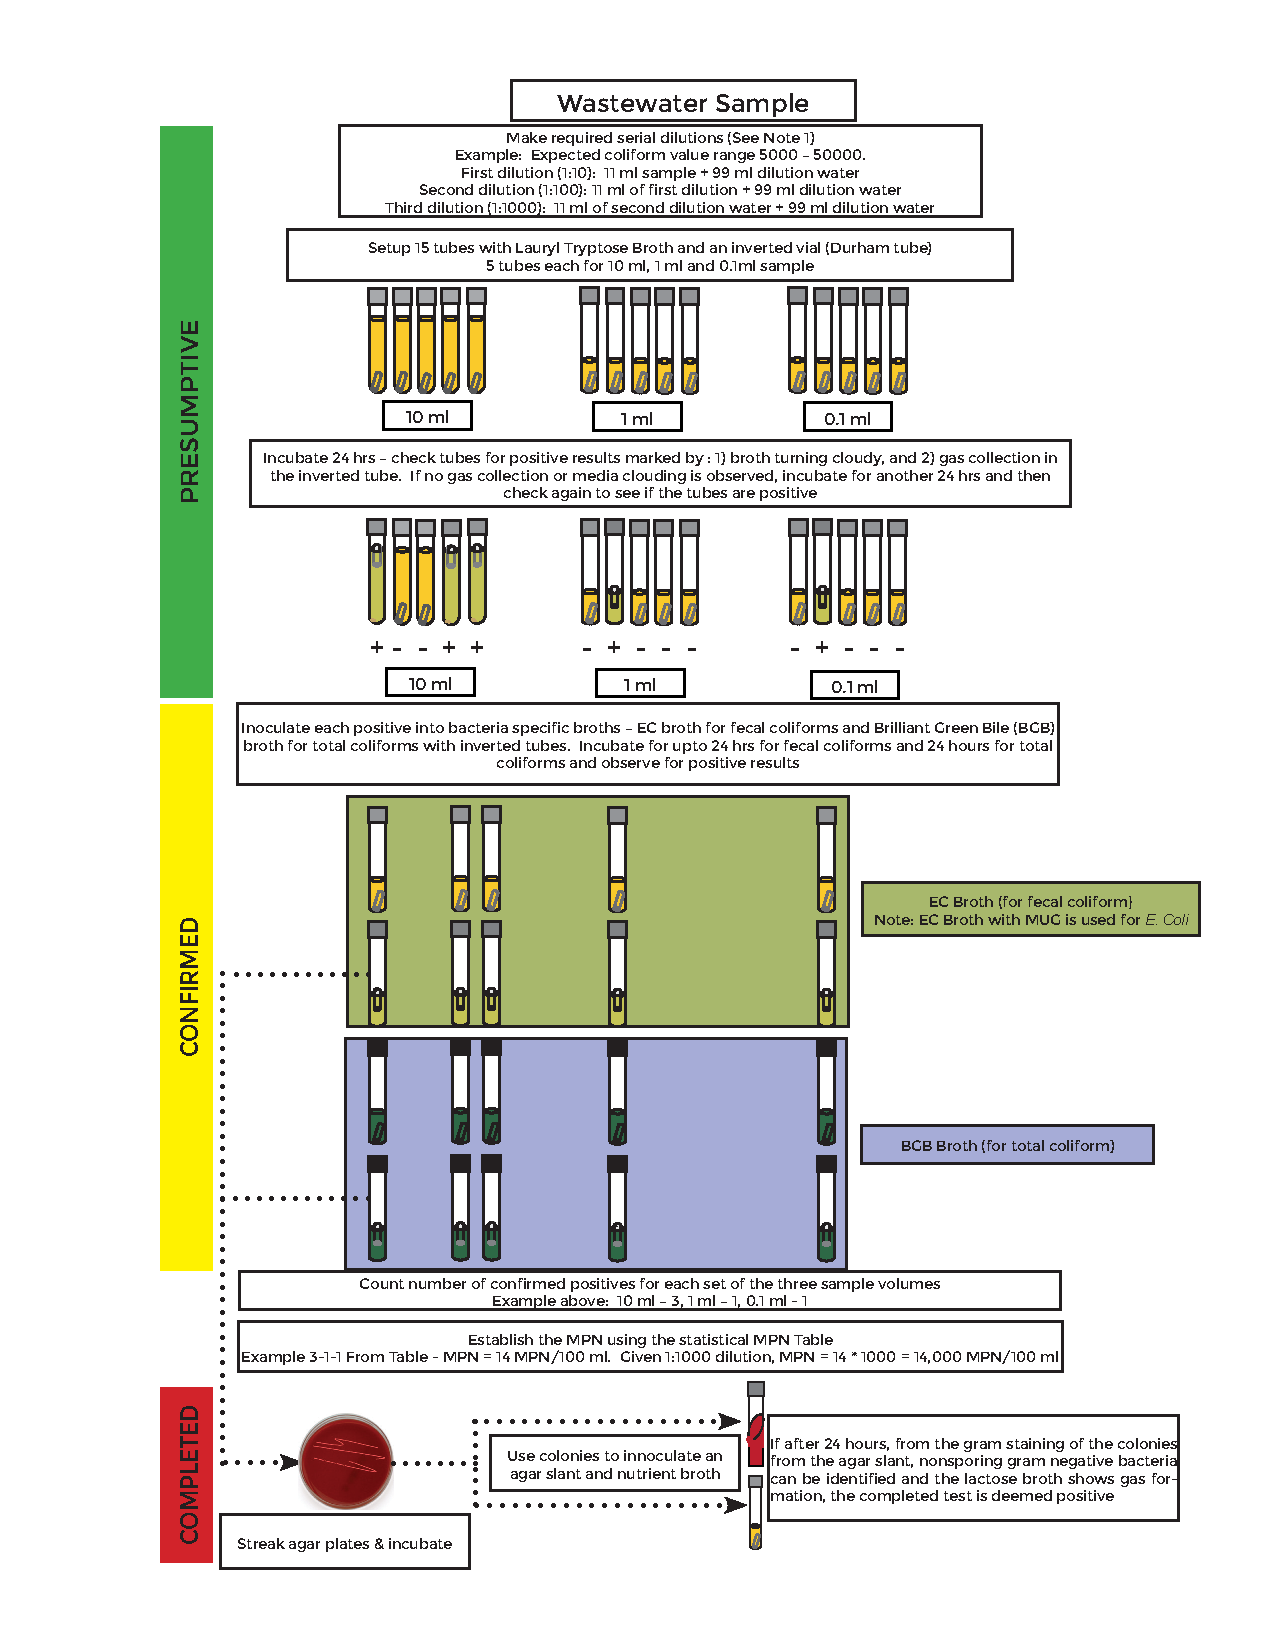
\includepdf[]{MTF.pdf}
%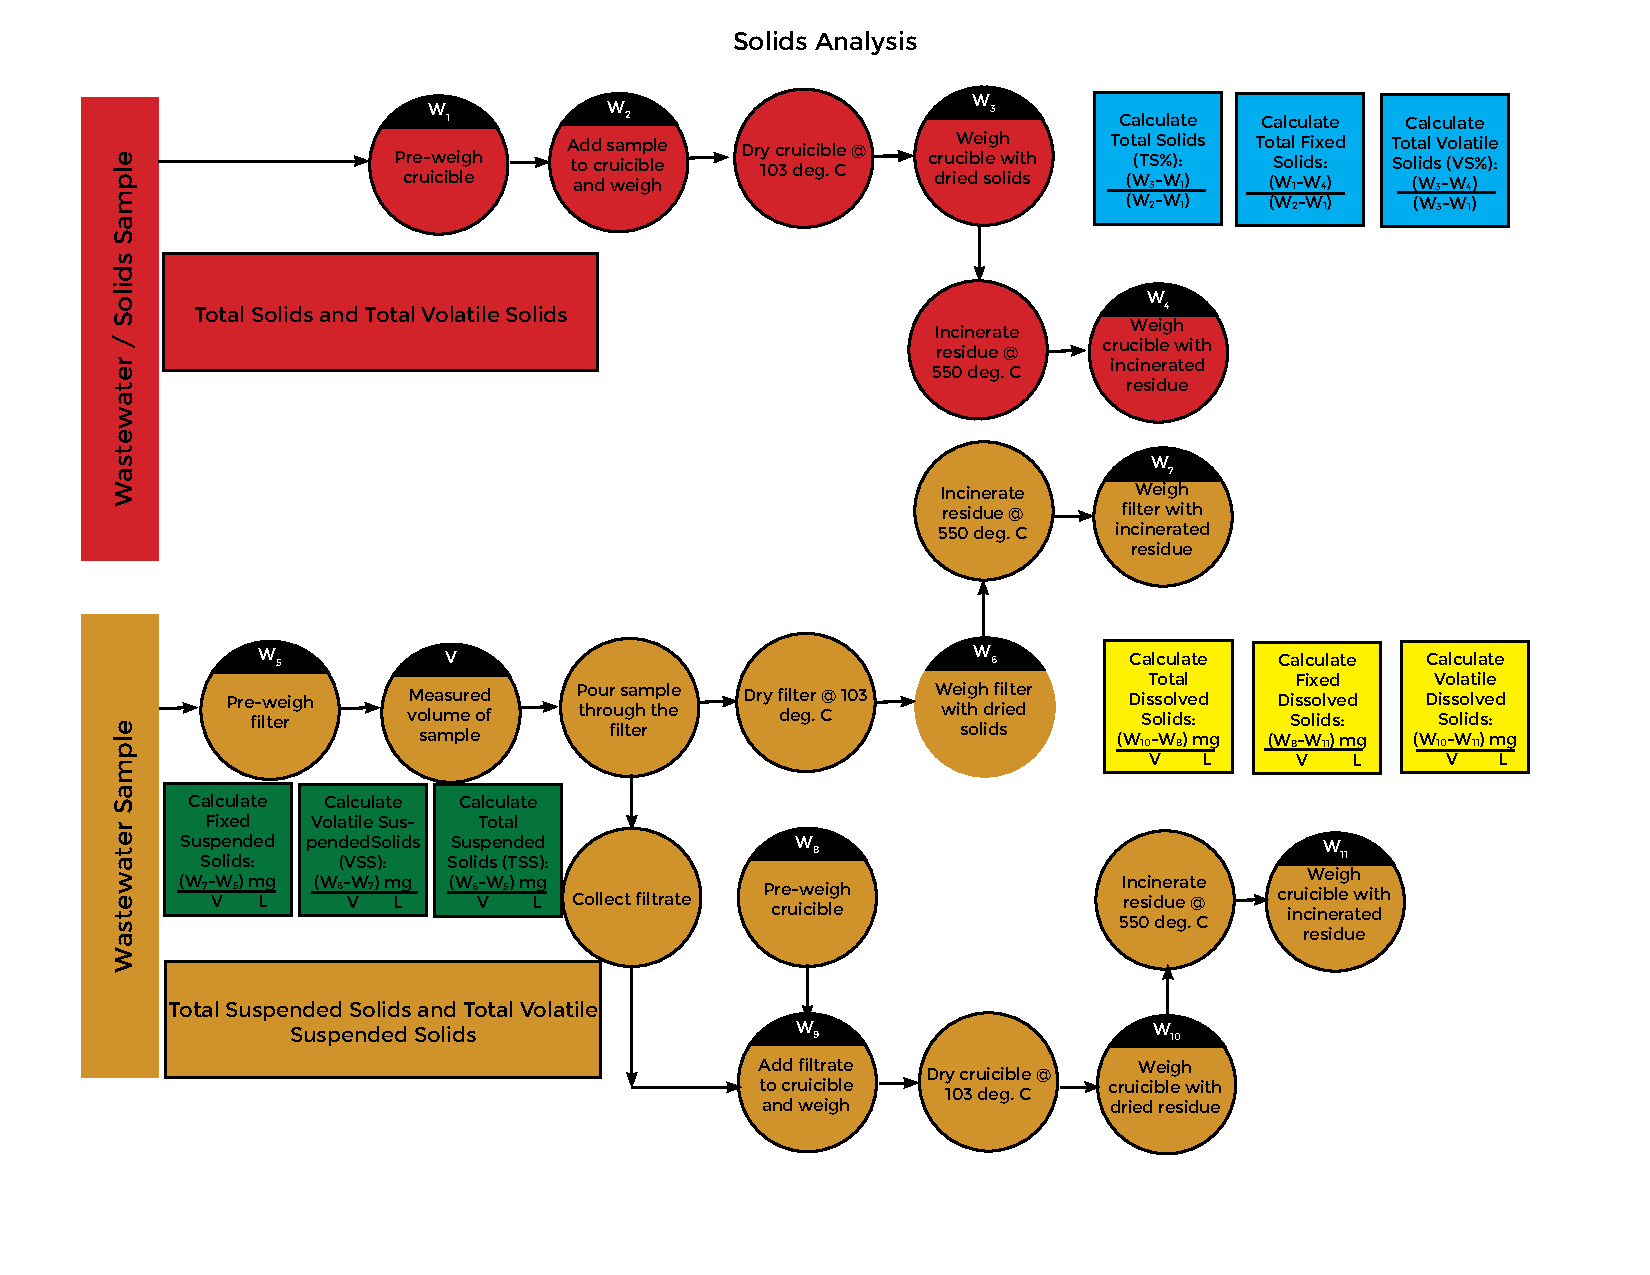
\includegraphics[scale=0.69]{LaboratorySolidsAnalysis4_01.pdf}
% \end{center}
% \end{landscape}
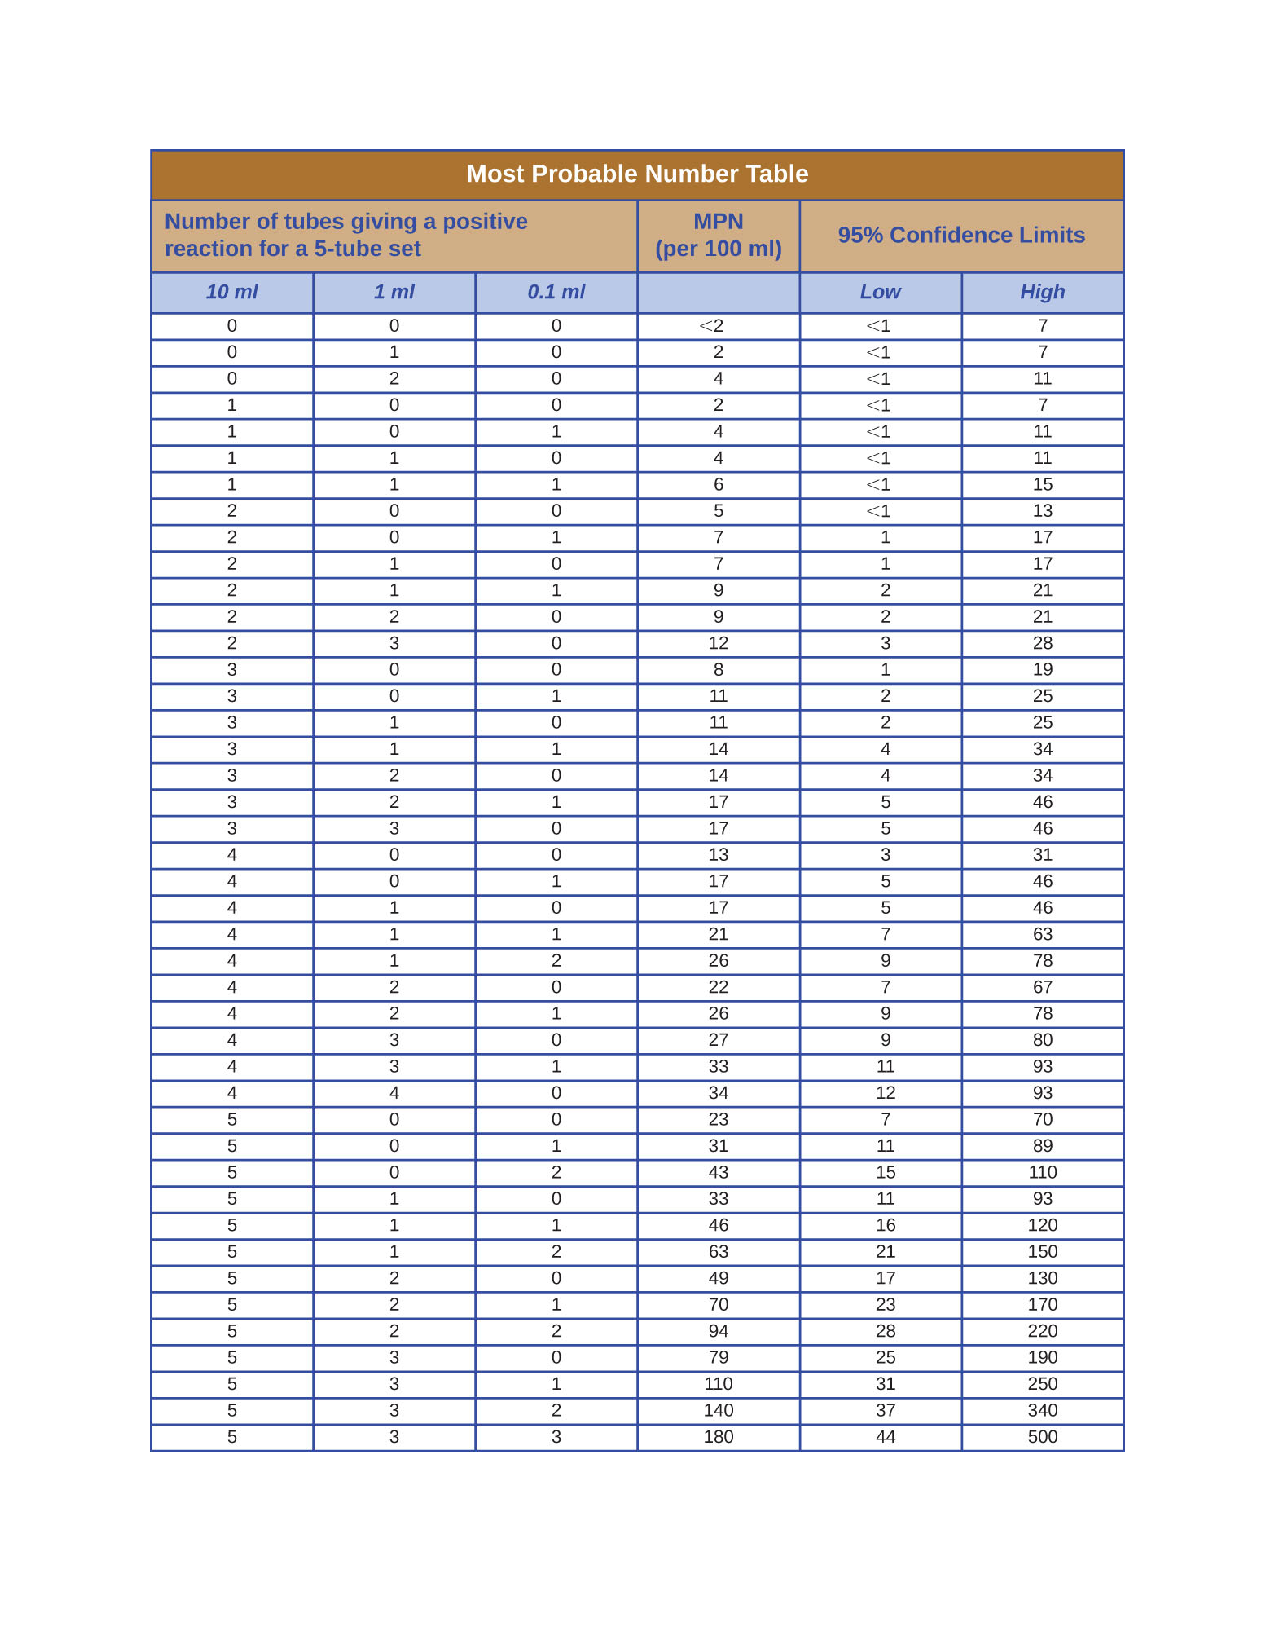
\includepdf[]{MTFTable.pdf}
\newpage
\subsection{The Membrane Filtration (MF) method}\index{The Membrane Filtration (MF) method}
This is a faster way to estimate bacterial populations in water.  In this method, an appropriate sample volume is passed through a membrane filter with a pore size small enough (0.45 micron) to retain the bacteria present. The filter is placed on an absorbent pad (in a petri dish) saturated with a culture medium that is selective for coliform growth. The petri dish containing the filter and pad is incubated, upside down, for 24 hours at the appropriate temperature. After incubation, the colonies that have grown are identified and counted using a low power microscope. A MUG medium is used for E- Coli.  If E. Coli is present, it will make the MUG fluorescent when viewed in UV light. 
\begin{center}
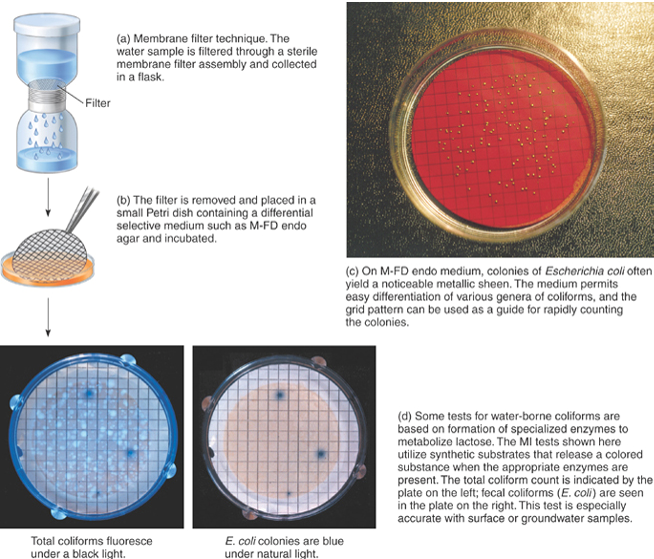
\includegraphics[scale=0.9]{LaboratoryMembraneFiltration}
\end{center}
\pagebreak

\subsection{Quanti-trays tests}\index{Quanti-trays tests}

This test used for the detection and quantification of specific microorganisms is being used increasingly mainly because it is a quicker test than the MTF.  Colilert and Enterolert are the quanti tray based tests for E. Coli and Enterococcus.  This method involve the use of specific enzymes and overcomes the drawbacks of the MTF which include false positives and negatives due to the more generic nature of the media used
\begin{center}
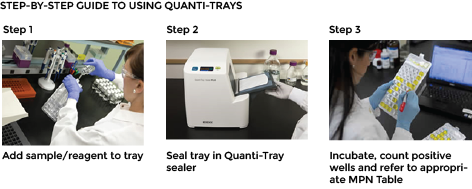
\includegraphics[scale=0.9]{LaboratoryQuantiTray}
\end{center}



%% \documentclass{article}
% %\usepackage[english]{babel}%
% \usepackage{graphicx}
% \usepackage{tabulary}
% \usepackage{tabularx}
% \usepackage[normalem]{ulem}
% \usepackage{cancel}
% \usepackage{tikz} 
% \usepackage{pdflscape}
% \usepackage{colortbl}
% \usepackage{lastpage}
% \usepackage{multirow}
% \usepackage{enumerate}
% \usepackage[shortlabels]{enumitem}
% \usepackage{color,soul}
% \usepackage{pdflscape}
% \usepackage{hyperref}
% %\usepackage[table]{xcolor}
% \usepackage{rotating}
% \usepackage{amsmath}
% \usepackage{fixltx2e}
% \usepackage{framed}
% \usepackage{mdframed}
% \usepackage[T1]{fontenc}
% \usepackage[utf8]{inputenc}
% \usepackage{textcomp}
% \usepackage{siunitx}
% \usepackage{ifthen}
% \usepackage{fancyhdr}
% \usepackage{gensymb}
% \usepackage{newunicodechar}
% \usepackage[document]{ragged2e}
% \usepackage[margin=1in,top=1.1in,headheight=57pt,headsep=0.1in]
% {geometry}
% \usepackage{ifthen}
% \usepackage{fancyhdr}
% \everymath{\displaystyle}
% \usepackage[document]{ragged2e}
% \usepackage{fancyhdr}
% \everymath{\displaystyle}
% \usepackage{empheq}

% \usepackage[most]{tcolorbox}

% \usepackage{booktabs} % Required for nicer horizontal rules in tables


% \usepackage{enumitem}

% %\usepackage[table,xcdraw]{xcolor}
% \usetikzlibrary{arrows}
% \linespread{2}%controls the spacing between lines. Bigger fractions means crowded lines%
% %\pagestyle{fancy}
% %\usepackage[margin=1 in, top=1in, includefoot]{geometry}
% %\everymath{\displaystyle}
% \linespread{1.3}%controls the spacing between lines. Bigger fractions means crowded lines%
% %\pagestyle{fancy}
% \pagestyle{fancy}
% \setlength{\headheight}{56.2pt}

% \definecolor{myblue}{rgb}{.8, .8, 1}
% \newcommand*\mybluebox[1]{%
% \colorbox{myblue}{\hspace{1em}#1\hspace{1em}}}

% \chead{\ifthenelse{\value{page}=1}{
\includegraphics[scale=0.3]{SCC}\\ \textbf \textbf Wastewater Constituents Analysis \& Laboratory Methods}}
% \rhead{\ifthenelse{\value{page}=1}{}{}}
% \lhead{\ifthenelse{\value{page}=1}{}{Wastewater Constituents Analysis \& Laboratory Methods}}
% \rfoot{\ifthenelse{\value{page}=1}{Module 1: WATR 048 - Spring 2019}{Module 1: WATR 048 - Spring 2019}}

% \lfoot{Shabbir Basrai}
% \cfoot{Page \thepage\ of \pageref{LastPage}}
% \renewcommand{\headrulewidth}{2pt}
% \renewcommand{\footrulewidth}{1pt}
% \begin{document}
% %\begin{empheq}[box=\mybluebox]{align}
% %a&=b\\
% %E&=mc^2 + \int_a^a x\, dx
% %\end{empheq}

% \newlist{steps}{enumerate}{1} % Defines "Steps" for enumerate as Step 1, Step 2 etc.
% \setlist[steps, 1]{label = Step \arabic*:} % Defines "Steps" for enumerate as Step 1, Step 2 etc.

% \setlist{nolistsep} % Reduce spacing between bullet points and numbered lists


%_______________________________________________________________________________________________________________________________________%
\chapterimage{MathCover.png} % Chapter heading image
\chapter{Wastewater Math Fundamentals}

\section{Units}\index{Units}

To measure any quantity or compare two physical quantities we need a universally accepted standard called Unit. The most common measurements involve measuring - length, weight and time.   International System of Units (SI), the modern form of the metric system is the globally accepted standard.  In the United States, it is customary to measure the physical quantities in English Engineering Units.\\
\vspace{0.5cm}
\begin{tabular}{c c c }
\hline
\multicolumn{3}{c}{\textbf{Fundamental Units}} \\
\hline
\textbf{Dimension} & \textbf{English Engineering Units} & \textbf{SI}\\
\hline
time & second (s) & second (s) \\
length & foot (ft) & meter (m)\\
mass & pound mass (lb) & kilogram\\
\end{tabular}\\

\vspace{0.5cm}

The measurement of any physical quantity is expressed in terms of a number - which is the quantity and a specific unit.  
Thus, a measurement of 5000 ft is basically 5000 of the of length as measured in ft.

Using the fundamental physical measurements, mathematical calculations can be made to measure other physical quantities such as area (ft$2$), volume (ft$3$), velocity (ft/s), flow (ft$3$/s), density (lbs/ft$3$).

Depending on the what is being measured or quantified, there are appropriate and customary units of measure - for example - miles and inches for length, gallons and acre-ft for volume and milligrams and tons for mass.
% \begin{enumerate}
% \definecolor{shadecolor}{RGB}{200, 200, 240}
% \begin{snugshade*}
%\section{Units and Unit Conversion}\index{Units and Unit Conversion}
% 	\item \noindent\textsc{Units and Unit Conversion}
% \end{snugshade*}
\subsection{Unit Conversions}\index{Unit Conversions}
Unit conversion is a process for changing the units of a measured quantity without changing its value.  It involves 
utilizing a \hl{conversion factor} which expresses the relationship between units that is used to change the units of a measured quantity without changing the value. Examples of conversion factors include:\\

\begin{center}
\renewcommand{\arraystretch}{1.5}
\vspace{0.5cm}
\begin{tabular}{l| c c }
\hline
\multicolumn{2}{c}{\textbf{Fundamental Units}} \\
\hline
\textbf{Dimension} & \textbf{Conversion Factor}\\[0.5cm]

\hspace{0.3cm}
time & $\dfrac{60 \enspace sec}{min}$, $\dfrac{1,440\enspace sec}{day}$\\[0.5cm]
length & $\dfrac{12 \enspace in}{ft}$, $\dfrac{5,280 \enspace ft}{mile}$\\[0.5cm]
mass & $\dfrac{2,000 \enspace lbs}{ton}$, $\dfrac{1000 \enspace gm}{mg}$\\
\end{tabular}\\
\begin{tabular}{l| c c }
\hline
\multicolumn{2}{c}{\textbf{Derived Units}} \\
\hline
\textbf{Dimension} & \textbf{Conversion Factor}\\[0.5cm]

\hspace{0.3cm}
area & $\dfrac{43,560 \enspace ft^2}{acre}$, $\dfrac{60 \enspace sec}{min}$\\[0.5cm]
volume & $\dfrac{27 \enspace ft^3}{yd}$, $\dfrac{7.48 \enspace gal}{ft^3}$\\
\end{tabular}\\
\end{center}
\vspace{0.5cm}

The numerator and the denominator of any conversion factor always equals one, they have the same value expressed in different units.

For converting one measurement unit to another.

Step 1:  Make sure the original unit is for the same measurement as the conversion unit.  So if the original unit is for area, say ft$^2$ the conversion unit can be another area unit such as in$^2$ or acre but it cannot be gallons as gallon is a unit of volume.

Step 2: Write down the conversion formula as:

$Quantity \enspace in \enspace converted \enspace unit = Quantity \enspace (\cancel{Original \enspace Unit}) *   Conversion  \enspace Factor \enspace  \dfrac{Conversion \enspace unit}{\cancel{Original \enspace unit}}$\\
\hspace{0.2cm}
Unit conversions may involve single factor where the original unit value is multiplied by the conversion factor to obtain the measured parameter in the converted (desired) unit.\\
For example:\\  
Converting 1000 $ft^3$ to cu. yards:\\

$1000 \cancel{ft^3}*\dfrac{cu.yards}{27\cancel{ft^3}} = 37 cu.yards$\\

Other unit conversions may require multiplying by known constants along with conversion factors.\\
For example:\\
\begin{enumerate}  

\item Converting 3.5 $ft^3/sec$ to MGD:\\
$\dfrac{3.5 \enspace \cancel{ft^3}}{\cancel{sec}} * \dfrac{7.48\cancel {\enspace gal}}{\cancel{ft^3}} * \dfrac{MG}{\enspace 10^6 \cancel{gal}}* \dfrac{1440*60 \enspace \cancel{sec}}{day}=  2.3 \enspace MGD$\\

\item Converting 1,000 L water to lbs:\\
$1000 \enspace \cancel{L}*\dfrac {\cancel{gal}}{3.785 \enspace \cancel{L}}*\dfrac{8.34 \enspace lbs}{\cancel{gal}}\enspace  = 2,203 \enspace lbs$\\
$(Note:8.34 \enspace lbs/gal \enspace is \enspace density \enspace of \enspace water - a \enspace constant)$\\ 

\end{enumerate}
\section{Fractions}\index{Fractions}
\begin{itemize}
\item A fraction is defined as part of whole.  If in a class there are 20 male students and 30 male students, the fraction of male students is $\dfrac{20}{50} or \dfrac{2}{5}$.
\item It is composed of three items: two numbers and a line.
\item The number on the top is called the numerator, the number on the bottom is called the denominator, and the line in between them means to divide. 
$$
\text { Divide } \longrightarrow \dfrac{3}{4} \quad \begin{aligned}
&\text { Numerator } \\
&\text { Denominator }
\end{aligned}
$$
\item A proper fraction is a fraction that has no whole number part and its numerator is smaller than its denominator. An improper fraction is a fraction that has a larger numerator than denominator and it represents a number greater than one.\\
Proper Fraction Examples: $\dfrac{1}{2}$, $\dfrac{5}{8}$, $\dfrac{11}{12}$\\
\vspace{0.2cm}
Improper Fraction Examples: $\dfrac{12}{2}$, $\dfrac{5}{2}$
\item Any whole number can be expressed as a fraction by placing a "1" in the denominator. For example:

2 is the same as $\dfrac{2}{1}$ and 45 is the same as $\dfrac{45}{1}$

\item Only fractions with the same denominator can be added/subtracted, and only the numerators are added/subtracted. For example:
$$
\dfrac{1}{8}+\dfrac{3}{8}=\dfrac{4}{8}  \enspace  \text {and},  \enspace \dfrac{7}{8}-\dfrac{3}{8}=\dfrac{4}{8}
$$

\item A fraction combined with a whole number is called a mixed number. For example:
$$
4 \dfrac{1}{8}, \enspace 16 \dfrac{2}{3}, \enspace  8 \dfrac{3}{4}, \enspace  45  \dfrac{1}{2} \text { and, } 12\dfrac{17}{32}
$$
These numbers are read, four and one eighth, sixteen and two thirds, eight and three fourths, forty-five and one half, and twelve and seventeen thirty seconds.\\
Mized numbers 

\item A fraction can be changed by multiplying the numerator and denominator by the same number. This does not change the value of the fraction, only how it looks. For instance:
$$
\dfrac{1}{2} \text { is the same as } \dfrac{1}{2} \times \dfrac{2}{2} \text { which is } \dfrac{2}{4}
$$

\item Steps to convert $\dfrac{17}{4}$ to a mixed number:
\begin{enumerate}[Step 1.]
\item How many times can 4 fit into 17? 4 because 4×4=16.  Thus, 4 becomes the whole number part
\item How much is left over in the numerator? 1 because $17-16=1$.  Thus, 1 becomes the numerator of the fractional part
\item $\dfrac{17}{4} = 4\dfrac{1}{4}$
\end{enumerate}
\vspace{0.2cm}
\item To turn a mixed number into an improper fraction, multiply the whole number part by the denominator and add the numerator. This becomes the new numerator over the original denominator.

Example: Converting 1.5 feet to fraction\\
$1.5ft=1\dfrac{1}{2}$\\
\vspace{0.2cm}
$1\dfrac{1}{2}=\dfrac{1*2+1}{2}=\dfrac{2+1}{2}=\dfrac{3}{2}$
\vspace{0.2cm}
\item A mixed value - say a circumference is given in feet and fraction of feet (say $7 \enspace 3/4$), needs to be converted to a fraction for calculation purposes.
\end{itemize}

\newpage
\section{Ratio}\index{Ratio}
\begin{itemize}
\item Ratio is used for comparing the size of two or more quantities.
\item Say if there are 10 red cubes and 5 pink marbles in a bag, the ratio $\dfrac{5}{10}$ is the ratio of pink marbles and red cubes.  It can also be represented by 5:10.
\item 5 lbs of chemical in 10 gallons solution is a ratio.  So is 30 miles per gallon.
\item Unlike fractions, ratio does not compare things that have the same units.
\end{itemize}
\section{Proportion}\index{Proportion}
\begin{itemize}
\item Two quantities are said to be in proportion if one changes, the other changes in a specific way.
\item Two quantities are said to be directly proportion, if the increase in one will \textbf{increase} the other value proportionally.  So if two quantities x and y are directly proportional, its ratio $\dfrac{x}{y}$ will be a fixed value. Thus for x$_1$ and y$_1$ different values of x and y respectively will be related by the equation $\dfrac{x}{y}=\dfrac{x_1}{y_1}$.  

\item This relationship is useful for calculating unknown values in water treatment calculations as in the following example: 

Knowing 200 lbs of bleach is needed to disinfect 5 MG of water at a treatment plant, calculate the lbs of bleach required to disinfect 3.2 MGD flow.

The ratio $\dfrac{200 \enspace pounds \enspace bleach}{5 MG}$ or 40 lbs bleach per MG is a constant.  Using this known proportion the lbs of bleach is needed to disinfect 3.2 MG at this plant can be calculated as follows by setting up the equation as:

$\dfrac{40 \enspace pounds \enspace bleach}{MG}=\dfrac{X}{3.2 \enspace MG}$ where X is the unknown lbs of bleach that is required to disinfect the 3.2 MG flow.

X can be calculated by cross multiplying the above equation: $X=\dfrac{3.2*40}{1}=128 \enspace lbs \enspace bleach$

\item Two quantities are said to be inversely proportional if the increase in one will decrease the second proportionally.  So if two quantities x and y are inversely proportional, its product $x * \text{y}$ will be a fixed value.  Examples of inversely proportional relationship include labor hours required to perform a certain task or time required to pump down a wetwell depending on the size of the pump.  An increase in assignment of labor hours will reduce the time required to perform the task or likewise putting a larger pump will reduce the time to pump down the wetwell.  So if two quantities x and y are inversely proportional, for x$_1$ and y$_1$ different values of x and y respectively will be related by the equation $x *y = x_1 * y_1$.

Application of inversely proportional relationship in water related calculation can be demonstration with the following example:

If it takes 20 minutes to pump a wet well down with one pump pumping at 125 gpm, then how long will it take if a 200 gpm pump is used?

As this is an inversely proportional relationship:

$(20 minutes * 125 gpm)=(X minutes * 200 gpm)$  where X is the unknown time to pump down the wetwell with the 200 gpm pump.

Solving for X: $X=\dfrac{20*125}{200}=12.5 minutes$
\end{itemize}

\newpage
\section{Decimals \& Powers of Ten}\index{Decimals \& Powers of Ten}
\begin{itemize}
\item A decimal is composed of two sets of numbers: the numbers to the left of the decimal are whole numbers, and numbers to the right of the decimal are parts of whole numbers, a fraction of a number.\\

\item The term used to express the fraction component is dependent on the number of characters to the right of the decimal.

\begin{itemize}
  \item The first character after the decimal point is tenths: $0.1$ - tenths

  \item The second character is hundredths: $0.01$ - hundredths

  \item The third character is thousandths: $0.001$ - thousandths
\end{itemize}

\item The term used to express the fraction component is dependent on the number of characters to the right of the decimal.

\begin{itemize}
  \item The first character after the decimal point is tenths: $0.1$ - tenths

  \item The second character is hundredths: $0.01$ - hundredths

  \item The third character is thousandths: $0.001$ - thousandths
\end{itemize}

\item Powers of 10 notation enables us to work with these very large and small quantities efficiently.
\item In water math, the most common application of this concept is related to parts per million (ppm) or parts per billion (ppb).
\item 1 million - 1,000,000 can be represented as 10$^6$.  Likewise, 1 billion - 1,000, 000,000 can be represented as 10$^9$
\item The sequence of powers of ten can also be extended to negative powers.
\item 1 part per million (1/1,000,000) can be written as 10$^-6$
\end{itemize}



\begin{table}[ht]
\begin{tabular}{|l|l|l|l|l|}
\hline
\multicolumn{1}{|c|}{\textbf{Name}} & \multicolumn{1}{c|}{\textbf{Power}} & \multicolumn{1}{c|}{\textbf{Number}} & \multicolumn{1}{c|}{\textbf{SI symbol}} & \multicolumn{1}{c|}{\textbf{SI prefix}} \\ \hline
one                                 & $10^0$& 1                                    &                                         &                                         \\ \hline
ten                                 & $10^1$                                   & 10                                   & da (D)                                  & deca                                    \\ \hline
hundred                             & $10^2$                                   & 100                                  & h (H)                                   & hecto                                   \\ \hline
thousand                            & $10^3$                                  & 1,000                                & k (K)                                   & kilo                                    \\ \hline
million                             & $10^6$                                   & 1,000,000                            & M                                       & mega                                    \\ \hline
billion                             & $10^9$                                  & 1,000,000,000                        & G                                       & giga                                    \\ \hline
tenth                               & $10^{-1}$                                 & 0.1                                  & d                                       & deci                                    \\ \hline
hundredth                           & $10^{-2}$                                  & 0.01                                 & c                                       & centi                                   \\ \hline
thousandth                          & $10^{-3} $                                 & 0.001                                & m                                       & milli                                   \\ \hline
millionth                           &$10^{-6} $                               & 0.000 001                            & $\mu$                                      & micro                                   \\ \hline
billionth                           & $10^{-9} $                               & 0.000 000 001                        & n                                       & nano                                    \\ \hline
\end{tabular}
\end{table}

\newpage

\section{Rounding and Significant Digits}\index{Rounding and Significant Digits}

\begin{itemize}
\item Significant digits (also called Significant Figures) are digits which give us useful information about the accuracy of a measurement and are related to rounding.
\item This concept is used to determine the direction to round a number (answer). The basic idea is that no answer can be more accurate than the least accurate piece of data used to calculate the answer.\\
\item Significant digits is the count of the numerals in a measured quantity (counting from the left) whose values are considered as known exactly, plus one more whose value could be one more or one less.\\
\item Rules for determining the number of significant digits:
\begin{enumerate}
\item All nonzero digits are significant:\\
1.234 g has 4 significant figures, and 1.2 g has 2 significant figures.
\item Zeroes between nonzero digits are significant:
1002 kg has 4 significant figures, 3.07 mL has 3 significant figures.
\item Zeroes to the left of the first nonzero digits are not significant; such zeroes merely indicate the position of the decimal point:
\SI{0.001}{\celsius} has only 1 significant figure, 0.012 g has 2 significant figures.
\item Zeroes to the right of a decimal point in a number are significant:
0.023 mL has 2 significant figures, 0.200 g has 3 significant figures.
\item When a number ends in zeroes that are not to the right of a decimal point, the zeroes are not necessarily significant:
190 miles may be 2 or 3 significant figures, 50,600 calories may be 3, 4, or 5 significant figures. The potential ambiguity in the last rule can be avoided by the use of standard exponential, or ”scientific,” notation. For example, depending on whether 3, 4, or 5 significant figures is correct, we could write 50,6000 calories as: $5.06*10^4$ calories (3 significant figures) $5.060*10^4$ calories (4 significant figures), or
$5.0600*10^4)$ calories (5 significant figures).
\end{enumerate}
\item Examples of significant figures:
% Please add the following required packages to your document preamble:
% \usepackage[normalem]{ulem}
% \useunder{\uline}{\ul}{}
% Please add the following required packages to your document preamble:
% \usepackage[normalem]{ulem}
% \useunder{\uline}{\ul}{}
\begin{table}[h]
\begin{tabular}{|p{16cm}|}
\hline
1000 has   one significant digit: only the 1 is interesting (only it tells us anything   specific); we don't know anything for sure about the hundreds, tens, or units   places; the zeroes may just be placeholders; they may have rounded something   off to get this value.                                     \\ \hline
1000.0 has five significant   digits: the ".0" tells us something interesting about the presumed   accuracy of the measurement being made; namely, that the measurement is   accurate to the tenths place, but that there happen to be zero tenths.                                                                \\ \hline
0.00035 has two significant   digits: only the 3 and 5 tell us something; the other zeroes are   placeholders, only providing information about relative size.                                                                                                                                                     \\ \hline
0.000350 has three significant   digits: the last zero tells us that the measurement was made accurate to that   last digit, which just happened to have a value of zero.                                                                                                                                          \\ \hline
1006 has four significant   digits: the 1 and 6 are interesting, and we have to count the zeroes, because   they're between the two interesting numbers.                                                                                                                                                           \\ \hline
560 has two significant   digits: the last zero is just a placeholder.                                                                                                                                                                                                                                             \\ \hline
560. : notice that   "point" after the zero! This has three significant digits, because   the decimal point tells us that the measurement was made to the nearest unit,   so the zero is not just a placeholder.                                                                                                   \\ \hline
560.0 has four significant   digits: the zero in the tenths place means that the measurement was made   accurate to the tenths place, and that there just happen to be zero tenths;   the 5 and 6 give useful information, and the other zero is between   significant digits, and must therefore also be counted. \\ \hline
\end{tabular}
\end{table}
\item Addition and Subtraction\\
\begin{itemize}
\item When you are \hl{adding or subtracting} a bunch of numbers and need to be concerned with significant figures, first add (or subtract) the numbers given in their entire format, and then round the final answer. \hl{When rounding the final answer after adding or subtracting, the answer must be written with the same significant figures as the least accurate decimal place given}.\\
\textbf{Example:} 13.214 + 234.6 + 7.0350 + 6.38\\
\begin{itemize}
\item 13.214 + 234.6 + 7.0350 + 6.38 = 261.2290\\
\item 234.6 is only accurate to the tenths place making it the least accurate number. My answer must be rounded to the same place as the least accurate number:\\
\item 261.2290 rounds to 261.2 (one decimal place)\\
\end{itemize}
\end{itemize}
\item Multiplication and Division\\
\begin{itemize}
\item When \hl{multiplying or dividing} multiple numbers you would do these calculations as normal. When the answer must be written in the appropriate significant figure your answer must \hl{round to the same number of significant figures as the least number of significant figures.}\\
\textbf{Example 1:}  Simplify, and round, to the appropriate number of significant digits \\
\begin{center}
16.235 x 0.217 x 5\\
\end{center}
\begin{enumerate}[Step 1.]
\item First off, 5 has only one significant figure, thus the final answer needs to be rounded to one significant digit\\
\item 16.235 x 0.217 x 5 = 17.614975\\
\item To round 17.614975 to one digit. I'll start with the 1 in the tens place. Immediately to its right is a 7, which is greater than 5, so 1 is rounded up to 2, and then replacing the 7 with a zero, and dropping the decimal point and everything after it.
\item 17.614975 rounds to 20\\
\end{enumerate}
\textbf{Example 2:}  Simplify, and round, to the appropriate number of significant figures\\
\begin{center}
0.00435 x 4.6
\end{center}
\begin{enumerate}[Step 1.]
\item 4.6 has only 2 significant figures, so the final answer should be rounded to two significant figures.
\item 0.00435 x 4.6 = 0.02001\\
\item 0.02001 would round to 0.020, which has 2 significant figures (0.020). The answer cannot be 0.02, because that value would have only one significant figure.\\
\end{enumerate}
\end{itemize}
\end{itemize}

\begin{itemize}
\item \emph{A number is rounded off by dropping one or more numbers from the right and adding zeroes, if necessary, to maintain the decimal point.} 
\item \emph{If the last figure dropped is 5 or more, increase the last retained figure by 1. If the last digit dropped is less than 5, do not increase the last retained figure.}
\end{itemize}
\newpage
\section{Averages}\index{Averages}
\begin{itemize}
\item Also known as \emph{arithmetic mean}, this value is arrived at by adding the quantities in a series and dividing the total by the number in the series.
\end{itemize}
Example 1: Find the average of the following series of numbers: 12,8,6,21,4,5 , 9 , and 12.\\
Adding the numbers together we get 77.\\
There are 8 numbers in this set.\\
Divide 77 by 8.\\

$\frac{77}{8}=9.6$ is the average of the set\\

Example 2:  Find the average of the set of daily turbidity data - 0.3,0.4,0.3,0.1,and 0.8\\
The total is 1.9.\\
There are 5 numbers in the set.\\
Therefore:
$$
\frac{1.9}{5}=0.38, \text { rounding off }=0.4
$$

\newpage
\section{Working with Percent}\index{Working with Percent}
\begin{itemize}
\item Percent expresses portions of the whole.  
\item \texthl{The whole is considered as 1 or 100\% and a part of the whole can be expressed as a percent.}
\textbf{Example:} If a tank is $1 / 2$ full, we say that it contains $50 \%$ of the original solution.
\item Percentage is written as a whole number with a \% sign after it. 
\item In a calculation, percent is expressed as a decimal. 
\item \texthl{The decimal form of a percent value is obtained by dividing the percent by 100.}\\
 \textbf{Example:} $11 \%$ is expressed as the decimal $0.11$, since $11 \%$ is equal to $11 / 100$. This decimal is obtained by dividing 11 by 100.
\item \texthl{To determine what percentage a part is of the whole, divide the part by the whole.}\\
\textbf{Example:} There are 80 water meters to read, Jim has finished 24 of them. What percentage of the meters have been read?\\
$$24 \div 80=0.30$$\\
The $0.30$ is converted to percent by multiplying the answer by 100.\\
$$0.30 \times 100=30 \%$$\\
Thus $30 \%$ of the 80 meters have been read.\\

\item \texthl{To find the percentage of a number, multiply the number by the decimal equivalent of the percentage given in the problem.}\\
\textbf{Example:}\\
What is $28 \%$ of $286 ?$\\

\begin{enumerate}[Step 1.]
\item Change the $28 \%$ to a decimal equivalent:  $$28 \% \div 100=0.28$$
\item Multiply $286 \times 0.28=80$\\
Thus $28 \%$ of 286 is 80.
\end{enumerate}

\item \texthl{To increase a value by a percent, add the decimal equivalent of the percent percent to " 1 " and multiply it times the number.}

\textbf{Example:} A filter bed will expand $25 \%$ during backwash. If the filter bed is 36 inches deep, how deep will it be during backwash?\\

\begin{enumerate}[Step 1.]
\item Change the percent to a decimal.
$$
25 \% \div 100=0.25
$$
\item Add the whole number 1 to this value.
$$
1+0.25=1.25
$$
\item Multiply times the value.
$$
36 \text { in } \times 1.25=45 \text { inches }
$$
\end{enumerate}
\end{itemize}
\subsection{Percentage Concentrations}
Above concepts are used for chemicals such as fluoride and hypochlorites - the strength of the product as used is commonly expressed as a percentage.

\textbf{Example 1:} A chlorine solution was made to have a $4 \%$ concentration. It is often desirable to determine this concentration in $\mathrm{mg} / \mathrm{L}$. This is relatively simple: the $4 \%$ is four percent of a million.

To find the concentration in $\mathrm{mg} / \mathrm{L}$ when it is expressed in percent, do the following:

\begin{enumerate}
  \item Change the percent to a decimal.
\end{enumerate}
$$
4 \% \div 100=0.04
$$

\begin{enumerate}
  \setcounter{enumi}{2}
  \item Multiply times a million.
\end{enumerate}
$$
0.04 \times 1,000,000=40,000 \mathrm{mg} / \mathrm{L}
$$
We get the million because a liter of water weighs $1,000,000 \mathrm{mg} .1 \mathrm{mg}$ in 1 liter is 1 part in a million parts ( $\mathrm{ppm}) .1 \%=10,000 \mathrm{mg} / \mathrm{L}$.


\textbf{Example 2:} How much $65 \%$ calcium hypochlorite is required to obtain 7 pounds of pure chlorine?\\
$65 \%$ implies that in every lb of calcium hypochlorite has $65 \%$ lbs of available chlorine.\\
\vspace{0.2cm}
Therefore, $\dfrac{0.65 \textrm{ lbs available chlorine}}{\textrm{lb of calcium hypochlorite}} $ or conversely $\dfrac{\textrm{lb of calcium hypochlorite}}{0.65 \textrm{ lbs available chlorine}}$\\
\vspace{0.2cm}
$\implies{\textrm{lbs calcium hypchlorite required}}=\dfrac{\textrm{lb of calcium hypochlorite}}{0.65 \cancel{\textrm{ lbs available chlorine}}}*\dfrac{7\cancel{\textrm{ lb of available chlorine}}}{}$\\
\vspace{0.2cm}
$=\boxed{10.8 \textrm{ lbs of calcium hypochlorite with } 65\%\textrm{available chlorine is required}}$


\newpage
\section{Area \& Volume}\index{Area \& Volume}
% \section{Area \& Volume}\index{Area \& Volume}

% \begin{snugshade*}
% 	\item \noindent\textsc{Area \& Volume}
% \end{snugshade*}

\begin{center}
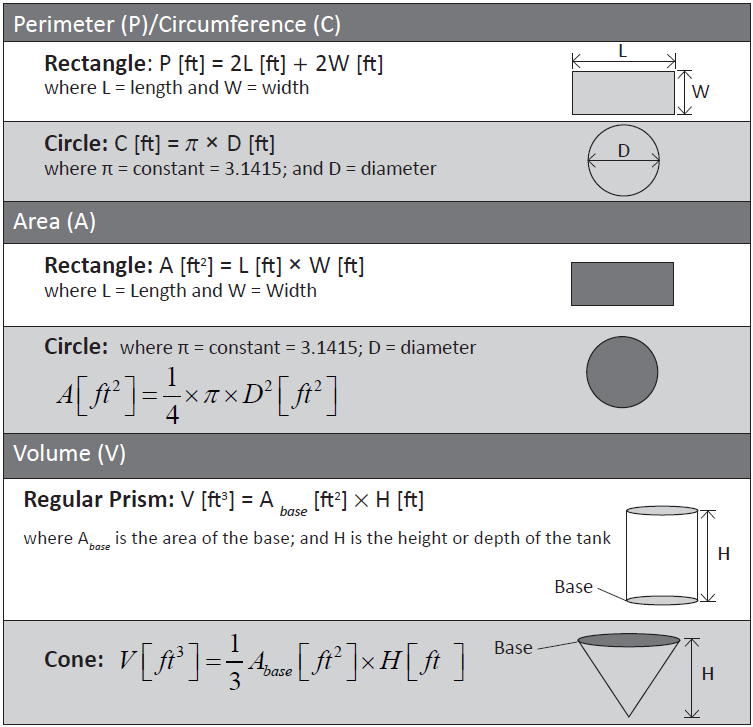
\includegraphics[scale=0.5]{Area&VolumeFormula}
\end{center}
\subsection{Example Problems}
% \hl{Example Problems}\\
\begin{enumerate}

\item The floor of a rectangular building is 20 feet long by 12 feet wide and the inside walls are 10 feet high. Find the total surface area of the inside walls of this building\\
Solution:\\
% \begin{center}
\begin{tikzpicture}
	%%% Edit the following coordinate to change the shape of your
	%%% cuboid
      
	%% Vanishing points for perspective handling
	\coordinate (P1) at (-7cm,1.5cm); % left vanishing point (To pick)
	\coordinate (P2) at (8cm,1.5cm); % right vanishing point (To pick)

	%% (A1) and (A2) defines the 2 central points of the cuboid
	\coordinate (A1) at (0em,0cm); % central top point (To pick)
	\coordinate (A2) at (0em,-2cm); % central bottom point (To pick)

	%% (A3) to (A8) are computed given a unique parameter (or 2) .8
	% You can vary .8 from 0 to 1 to change perspective on left side
	\coordinate (A3) at ($(P1)!.8!(A2)$); % To pick for perspective 
	\coordinate (A4) at ($(P1)!.8!(A1)$);

	% You can vary .8 from 0 to 1 to change perspective on right side
	\coordinate (A7) at ($(P2)!.7!(A2)$);
	\coordinate (A8) at ($(P2)!.7!(A1)$);

	%% Automatically compute the last 2 points with intersections
	\coordinate (A5) at
	  (intersection cs: first line={(A8) -- (P1)},
			    second line={(A4) -- (P2)});
	\coordinate (A6) at
	  (intersection cs: first line={(A7) -- (P1)}, 
			    second line={(A3) -- (P2)});

	%%% Depending of what you want to display, you can comment/edit
	%%% the following lines

	%% Possibly draw back faces

	\fill[gray!40] (A2) -- (A3) -- (A6) -- (A7) -- cycle; % face 6
	\node at (barycentric cs:A2=1,A3=1,A6=1,A7=1) {\tiny Floor=W*L};
	
	\fill[gray!50] (A3) -- (A4) -- (A5) -- (A6) -- cycle; % face 3
	\node at (barycentric cs:A3=1,A4=1,A5=1,A6=1) {\tiny Wall - W*H};
	
	\fill[gray!10, opacity=0.2] (A5) -- (A6) -- (A7) -- (A8) -- cycle; % face 4
	\node at (barycentric cs:A5=1,A6=1,A7=1,A8=1) {\tiny Wall - L*H};
	
	\fill[gray!10,opacity=0.5] (A1) -- (A2) -- (A3) -- (A4) -- cycle; % f2
	\node at (barycentric cs:A1=1,A2=1,A3=1,A4=1) {\tiny Wall - L*H};
	
	\fill[gray!40,opacity=0.2] (A1) -- (A4) -- (A5) -- (A8) -- cycle; % f5
	\node at (barycentric cs:A1=1,A4=1,A5=1,A8=1) {\tiny Ceiling=W*L};	
	
	\draw[thick,dashed] (A5) -- (A6);
	\draw[thick,dashed] (A3) -- (A6);
	\draw[thick,dashed] (A7) -- (A6);

	%% Possibly draw front faces

	%\fill[orange] (A1) -- (A8) -- (A7) -- (A2) -- cycle; % face 1
	\node at (barycentric cs:A1=1,A8=1,A7=1,A2=1) {\tiny Wall - W*H};
	


	%% Possibly draw front lines
	\draw[thick] (A1) -- (A2);

	\draw[<->] (-1.8,0.38) -- (-1.8,-1.3)node [midway, above=-1.8mm] {\hspace{-1.3cm}\tiny Height=10'};
	\draw[<->] (-1.6,-1.4) -- (-.3,-2.1)node [midway, above=-2.6mm] {\hspace{-1.3cm}\tiny Length=20'};
	\draw[<->] (2.6,-1.13) -- (0.2,-2.2)node [midway, below=.6mm] {\hspace{1.2cm}\tiny Width=12'};
	\draw[thick] (A3) -- (A4);
	\draw[thick] (A7) -- (A8);
	\draw[thick] (A1) -- (A4);
	\draw[thick] (A1) -- (A8);
	\draw[thick] (A2) -- (A3);
	\draw[thick] (A2) -- (A7);
	\draw[thick] (A4) -- (A5);
	\draw[thick] (A8) -- (A5);
	
	% Possibly draw points
	% (it can help you understand the cuboid structure)
%	\foreach \i in {1,2,...,8}
%	{
%	  \draw[fill=black] (A\i) circle (0.15em)
%	    node[above right] {\tiny \i};
%	}
	% \draw[fill=black] (P1) circle (0.1em) node[below] {\tiny p1};
	% \draw[fill=black] (P2) circle (0.1em) node[below] {\tiny p2};
\end{tikzpicture}\\
% \end{center}
2 Walls W*H + 2 Walls L*H= $2*12*10ft^2 + 2*20*10ft^2$\\
$=240+400=\boxed{640ft^2}$

2 Walls W*H + 2 Walls L*H + Floor + Ceiling= $2*12*10ft^2 + 2*20*10ft^2 + 2*12*20ft^2$\\
$=240+400+480=\boxed{1,120ft^2}$
\end{enumerate}
\section{Concentration}\index{Concentration}

Concentration is typically expressed as mg/l which is the weight of the constituent (mg) in 1 l (liter) of solution (wastewater).  As 1 l of water weighs 1 million mg, a concentration of 1 mg/l implies 1 mg of constituent per 1 million mg of water or one part per million (ppm).   \textbf{Thus, mg/l and ppm are synonymous.}\\  
Sometimes the constituent concentration is expressed in terms of percentage.\\
\vspace{6pt}
For example:  sludge containing 5\% solids or a 12.5\% chlorine concentration solution.\\
\vspace{6pt}
As one liter of water weighs 1,000,000 mg, one percent of that weight is 10,000 mg.  So 1\% solids implies 10,000 mg of solids per liter or 10,000 mg/l or 10,000 ppm.\\
\vspace{6pt}
$1\% concentration = 10,000 \enspace ppm \enspace or \enspace\dfrac{mg}{l}$\\
\vspace{6pt}
$0.1\% concentration = 1,000 \enspace ppm \enspace or \enspace \dfrac{mg}{l}$\\
\vspace{6pt}
$0.01\% concentration = 100 \enspace ppm \enspace or \enspace \dfrac{mg}{l}$\\
\vspace{6pt}
$10\% concentration = 100,000 \enspace ppm \enspace or \enspace \dfrac{mg}{l}$\\
\vspace{6pt}
$5\% concentration = 50,000 \enspace ppm \enspace or \enspace \dfrac{mg}{l}$\\
\vspace{6pt}
$A \enspace  12.5\% \enspace bleach \enspace solution \enspace contains \enspace 12.5\% \enspace or \enspace 125,000 \enspace \dfrac{mg}{l} \enspace of \enspace \enspace active \enspace chlorine $

\section{Process Removal Efficiency}\index{Process Removal Efficiency}

% \section{Process Removal Efficiency}\index{Process Removal Efficiency}
% \begin{snugshade*}
% 	\item \noindent\textsc{Process Removal Efficiency}
% \end{snugshade*}
\begin{itemize}
\item Process removal rate or removal efficiency is the percentage of the inlet concentration removed.  
\item It is used for quantifying the pollutant removal during wastewater treatment and is established based upon the amount of a particular wastewater constituent entering and leaving a treatment process.

\item $Process \enspace Removal \enspace Rate \enspace (\%) = \dfrac{Pollutant \enspace  In-Pollutant\enspace  Out}{Pollutant \enspace In}*100$\\

\item If 10 units of a pollutant are entering a process and 8 units of pollutant are leaving (process removes 2 units), then the process removal rate for that pollutant is (10-8)/10*100=20\%.  In this example the process is 20\% efficient in removing that particular pollutant.

\item The amount of pollutant can be measured in terms of concentration (mg/l) or in terms of mass loading (lbs).  The pounds formula is used for calculating the mass loadings.  
\end{itemize}
The above example is for calculating the removal efficiency using the inlet and outlet concentrations or mass loading.\\
The methods below can be used for calculating either the inlet or outlet pollutant concentrations, if the removal efficiency and the corresponding inlet or outlet concentrations are given. 


\hl{Case 1:  Calculating outlet conc. (X) given the inlet conc. and removal efficiency (RE\%):}

\tikzstyle{block} = [rectangle, draw, fill=red!40, 
    text width=6em, text centered, rounded corners, minimum height=3em]
\tikzstyle{arrow} = [draw, -latex']
\begin{figure}[!h]
\centering
\begin{tikzpicture}[node distance =1.5cm, auto]
    \draw ++(0,0) node [block] (Process) {Process};
   \node[node distance=1.9in] (dummy_in) [left of=Process] {In};
   \node[node distance=1.9in] (dummy_out) [right of=Process] {Out};
	\node (Removal) [below of=Process, yshift=-0in] {${Removal \enspace Efficiency=RE\% \enspace (Given)}$};
    \path [arrow] (dummy_in)-- (Process)  node [above] {\hspace{-5.8cm}$A \enspace mg/l \enspace (Given) $} node [below] {\hspace{-5.8cm}$100 \enspace mg/l$};
    \path [arrow] (Process) -- (dummy_out)  node [above] {\hspace{-4cm}$X \enspace mg/l \enspace (Unknown)$} node [below] {\hspace{-3.9cm}($100-RE\%)\enspace mg/l$};
   \draw[arrow] (Process) -- (Removal);
\end{tikzpicture}
\end{figure}
Using the fact that if the inlet concentration was 100 mg/l, the outlet concentration would be 100 minus the removal efficiency.\\
Setup the equation as:  $\dfrac{Out}{In}: \enspace \dfrac{X \enspace mg/l}{A \enspace mg/l}=\dfrac{100-RE\%}{100}$\\
Calculate X using cross multiplication - if $\dfrac{A}{B}=\dfrac{C}{D} \implies A=B*\dfrac{C}{D}$:\\
$X \enspace mg/l=A \enspace mg/l*\dfrac{100-RE\%}{100}$\\


\hl{Case 2:  Calculating inlet conc. (X) given the outlet conc. and removal efficiency (RE\%):}

\begin{figure}[!h]
\centering
\begin{tikzpicture}[node distance =1.5cm, auto]
    \draw ++(0,0) node [block] (Process) {Process};
   \node[node distance=1.9in] (dummy_in) [left of=Process] {In};
   \node[node distance=1.9in] (dummy_out) [right of=Process] {Out};
	\node (Removal) [below of=Process, yshift=-0in] {$Removal \enspace Efficiency=RE\% \enspace (Given)$};
    \path [arrow] (dummy_in)-- (Process)  node [above] {\hspace{-5.8cm}$X \enspace mg/l \enspace (Unknown)$} node [below] {\hspace{-5.8cm}$100 \enspace mg/l$};
    \path [arrow] (Process) -- (dummy_out)  node [above] {\hspace{-4cm}$A \enspace mg/l \enspace (Given)$} node [below] {\hspace{-3.9cm}($100-RE\%)\enspace mg/l$};
   \draw[arrow] (Process) -- (Removal);
\end{tikzpicture}
\end{figure}
Using the fact that if the inlet concentration was 100 mg/l, the outlet concentration would be 100 minus the removal efficiency.\\
Setup the equation as:  $\dfrac{In}{Out}: \enspace \dfrac{X \enspace mg/l}{A \enspace mg/l}=\dfrac{100}{100-RE\%}$\\
\vspace{0.3cm}
Calculate X using cross multiplication - if $\dfrac{A}{B}=\dfrac{C}{D} \implies A=B*\dfrac{C}{D}$:\\
$X \enspace mg/l=A \enspace mg/l*\dfrac{100}{100-RE\%}$\\

\vspace{0.4cm}
\subsection{Example Problems}
% \hl{Example Problems:}\\

\begin{enumerate}

\item What is the \% removal efficiency if the influent concentration is 10 mg/L and the effluent concentration is 2.5 mg/L?\\
$Removal \enspace Rate (\%) = \dfrac{In-Out}{In}*100 \implies \dfrac{10-2.5}{10}*100=\boxed{75\%}$



\item Calculate the outlet concentration if the inlet concentration is 80 mg/l and the process removal efficiency is 60\%\\
Solution:\\

\tikzstyle{block} = [rectangle, draw, fill=red!40, 
    text width=6em, text centered, rounded corners, minimum height=3em]
\tikzstyle{arrow} = [draw, -latex']
\begin{figure}[!h]
\centering
\begin{tikzpicture}[node distance =1.5cm, auto]
    \draw ++(0,0) node [block] (Process) {Process};
   \node[node distance=1.5in] (dummy_in) [left of=Process] {In};
   \node[node distance=1.5in] (dummy_out) [right of=Process] {Out};
	\node (Removal) [below of=Process, yshift=-0in] {$Removal \enspace Efficiency=60\%$};
    \path [arrow] (dummy_in)-- (Process)  node [above] {\hspace{-4.39cm}$80mg/l$} node [below] {\hspace{-4.39cm}$100mg/l$};
    \path [arrow] (Process) -- (dummy_out)  node [above] {\hspace{-3.cm}$Xmg/l$} node [below] {\hspace{-3cm}40mg/l};
   \draw[arrow] (Process) -- (Removal);
\end{tikzpicture}
%\caption[MFCC]{Diagrama en bloques del cálculo de las MFCC para un frame.}
%\label{MFCC}
\end{figure}

$\dfrac{Out}{In} \enspace:\enspace\dfrac{Actual \enspace Outlet (X)}{80}=\dfrac{100-60}{100}$\\
$\implies \dfrac{Actual \enspace Outlet (X)}{80} =0.4$\\
$\implies Actual \enspace  Outlet (X) = 0.4 * 80 = \boxed{32 mg/l}$\\


\item Calculate the inlet concentration if the outlet concentration is 80 mg/l and the process removal efficiency is 60\%\\

\tikzstyle{block} = [rectangle, draw, fill=red!40, 
    text width=6em, text centered, rounded corners, minimum height=3em]
\tikzstyle{arrow} = [draw, -latex']
\begin{figure}[!h]
\centering
\begin{tikzpicture}[node distance =1.5cm, auto]
    \draw ++(0,0) node [block] (Process) {Process};
   \node[node distance=1.5in] (dummy_in) [left of=Process] {In};
   \node[node distance=1.5in] (dummy_out) [right of=Process] {Out};
	\node (Removal) [below of=Process, yshift=-0in] {$Removal \enspace Efficiency=60\%$};
    \path [arrow] (dummy_in)-- (Process)  node [above] {\hspace{-4.39cm}$Xmg/l$} node [below] {\hspace{-4.39cm}$100mg/l$};
    \path [arrow] (Process) -- (dummy_out)  node [above] {\hspace{-3.cm}80mg/l} node [below] {\hspace{-3cm}40mg/l};
   \draw[arrow] (Process) -- (Removal);
\end{tikzpicture}
\end{figure}

$\dfrac{In}{Out} \enspace : \enspace \dfrac{Actual \enspace inlet \enspace  (X)}{80}=\dfrac{100}{100-60}\implies \dfrac{Actual \enspace inlet \enspace  (X)}{80}=2.5$\\    
Rearranging the equation:   $Actual \enspace inlet (X)=2.5*80 = \boxed{200 mg/l}$\\

\item If a plant removes 35\% of the influent BOD in the primary treatment and 85\% of the remaining BOD in the secondary system, what is the BOD of the raw wastewater if the BOD of the final effluent is 20mg/l\\
Solution:\\

\begin{figure}[!h]
\centering
\begin{tikzpicture}[node distance =1.5cm, auto]
    \draw ++(0,0) node [block] (Primary) {Primary};
    
   \node[node distance=1.9in] (dummy_in) [left of=Primary] {Influent BOD};
   \node[node distance=1.9in] (dummy_out) [right of=Primary] {Primary BOD Out};
	\node (Removal) [below of=Primary, yshift=-0in] {$Removal \enspace Efficiency=35\% $};
    \path [arrow] (dummy_in)-- (Primary)  node [above] {\hspace{-4.8cm}$X \enspace mg/l \enspace$} node [below] {};
    \path [arrow] (Primary) -- (dummy_out)  node [above] {\hspace{-4.9cm}$0.65X \enspace mg/l$} node [below] {};
   \draw[arrow] (Process) -- (Removal);
\end{tikzpicture}
\end{figure}


\begin{figure}[!h]
\centering
\begin{tikzpicture}[node distance =1.5cm, auto]
    \draw ++(0,0) node [block] (Secondary) {Secondary};
    
   \node[node distance=1.9in] (dummy_in) [left of=Secondary] {Primary BOD Out};
   \node[node distance=1.9in] (dummy_out) [right of=Secondary] {Secondary BOD Out};
	\node (Removal) [below of=Secondary, yshift=-0in] {$Removal \enspace Efficiency=85\% $};
    \path [arrow] (dummy_in)-- (Secondary)  node [above] {\hspace{-4.8cm}$0.65X \enspace mg/l \enspace$} node [below] {\hspace{-5cm}$100 \enspace mg/l$};
    \path [arrow] (Secondary) -- (dummy_out)  node [above] {\hspace{-4.9cm}$20 \enspace mg/l$} node [below] {\hspace{-4.9cm}$15 \enspace mg/l$};
   \draw[arrow] (Process) -- (Removal);
\end{tikzpicture}
\end{figure}
\vspace{0.3cm}
For the Secondary process:\\
$\dfrac{In}{Out}: \enspace \dfrac{0.65X}{20}=\dfrac{100}{15} \implies X \enspace mg/l=\dfrac{100*20}{15*0.65}=\boxed{205 \enspace mg/l}$\\

\vspace{0.3cm}
Alternate Solution \#1

$\xrightarrow[
				\text{X}\dfrac{mg}{l}
			]
			{
			\text{Influent BOD}
			}
 \boxed{Primary}
 \xrightarrow[
 				\text{X-0.35X=X*(1-0.35)=0.65X}\dfrac{mg}{l}
 			]
 			{
 			\text{Primary Effluent BOD}
 			}
 \boxed{Secondary}
 \xrightarrow[
				\text{0.65X-0.5525X=(0.65-0.5525)X=0.0975X }
			 ]
			{
			\text{Secondary Effluent BOD}
			}
$\\
\hspace{2.8cm}$\downarrow$ {\tiny(0.35X)BOD Removed}\hspace{3.2cm}$\downarrow$ {\tiny(0.65*0.85)X = 0.5525X BOD Removed}\\
$\implies 0.0975X=20 \implies X=\dfrac{20}{0.0975}=\boxed{205\dfrac{mg}{l}}$\\

\vspace{0.3cm}

Alternate Solution \#2:\\
$\xrightarrow[\text{X}\dfrac{mg}{l}]{\text{Influent BOD}}\boxed{Primary}\xrightarrow[\text{0.65X}]{\text{Primary Effluent BOD}}\boxed{Secondary}\xrightarrow[\text{(0.65*0.15)X}]{\text{Secondary Effluent BOD}}$\\
\hspace{2.8cm}$\downarrow$ {\tiny(0.35X)BOD Removed}\hspace{2.2cm}$\downarrow$ {\tiny(0.65X*0.85)BOD Removed}\\

Primary Effluent BOD = Influent BOD * (1-Primary BOD Removal), and\\
Secondary Effluent BOD=[Primary Effluent BOD]*(1-Secondary BOD Removal)\\
Secondary Eff. BOD=[Influent BOD * (1-Primary BOD Removal)]*(1-Secondary BOD Removal)\\

Therefore, 20 = [X*(1-0.35)] * (1-0.85)= X*0.65*0.15\\
$\implies 20 \enspace \dfrac{mg}{l}= 0.0975X \implies X=\dfrac{20}{0.0975}=\boxed{205 \enspace \dfrac{mg}{l}}$

\end{enumerate}
\section{Pumping}\index{Pumping}
% \section{Pumping}\index{Pumping}
% \pagebreak
% \begin{snugshade*}
% 	\item \noindent\textsc{Pumping}
% \end{snugshade*}
For Grades I \& II, pumping rate problems include the following:
% \begin{enumerate}
% \definecolor{shadecolor}{RGB}{225, 235, 235}
% \begin{snugshade*}
% \item \noindent\textsc{Calculating volume pumped in a given time interval given the pump flow rate\\}
% \end{snugshade*}
\subsection{Calculating volume pumped given the pump flow rate}\index{Calculating volume pumped given the pump flow rate}

\textbf{Method:\\}
\hspace{1cm}Step 1. Multiply the pump flow rate by the time interval\\
\textbf{Make sure:}
\begin{itemize}
\item The time units - in the given time interval and in the pump flow rate match
\end{itemize}
\subsection{Calculating time to pump a certain volume}\index{Calculating time to pump a certain volume}
% \begin{snugshade*}
% \item \noindent\textsc{Calculating time to pump a certain volume given the pump flow rate\\}
% \end{snugshade*}
\textbf{Method:}
\hspace{1cm}Step 1. Calculate the total volume pumped\\
\hspace{1cm}Step 2.	Divide the total volume by the pump flow rate\\
\textbf{Make sure:}
\begin{itemize}
\item The volume units - in the volume that needs to be pumped and in the pump flow rate match
\item The time unit in the pump flow rate needs to be converted to the time unit that you need the answer in
\end{itemize}
% \end{enumerate}

\section{Example Problems}
% \hl{Example Problems:}\\

\begin{enumerate}

\item A sludge pump is set to pump 5 minutes each hour. It pumps at the rate of 35 gpm. How many gallons of sludge are pumped each day?\\
Solution:\\
$\dfrac{35 \enspace gal \enspace sludge}{\cancel{min}}*\dfrac{5 \enspace \cancel{min}}{\cancel{hr}} *\dfrac{24 \enspace \cancel{hr}}{day}=\boxed{\dfrac{4,200 \enspace gallons}{day}}$\\
\vspace{0.5cm}

\item A sludge pump operates 5 minutes each 15 minute interval.  If the pump capacity is 60 gpm, how many gallons of sludge are pumped daily?

$\dfrac{60 \enspace gal \enspace sludge}{\xcancel{min}}*\dfrac{5 \enspace \xcancel{min}}{15 \enspace \cancel{min}}*1440\dfrac{\cancel{min}}{day}=\boxed{\dfrac {28,800 \enspace gal \enspace sludge }{day}}$\\

\item Given the tank is 10ft wide, 12 ft long and 18 ft deep tank including 2 ft of freeboard when filled to capacity. How much time (minutes) will be required to pump down this tank to a depth of 2 ft when the tank is at maximum capacity using a 600 GPM pump\\
Solution:\\
\vspace{0.5cm}


\begin{tikzpicture}

\pgfmathsetmacro{\cubexx}{4}
\pgfmathsetmacro{\cubeyy}{1.5}
\pgfmathsetmacro{\cubezz}{2}
\pgfmathsetmacro{\cubex}{4}
\pgfmathsetmacro{\cubey}{0.5}
\pgfmathsetmacro{\cubez}{2}
\pgfmathsetmacro{\cubexxx}{4}
\pgfmathsetmacro{\cubeyyy}{4}
\filldraw [fill=cyan!10!white, draw=black] (0,-\cubey,0) -- ++(-\cubexx,0,0) -- ++(0,-\cubeyy,0) -- ++(\cubexx,0,0) -- cycle ;
\filldraw [fill=cyan!0!white, draw=black] (0,-\cubey,0) -- ++(0,0,-\cubezz) -- ++(0,-\cubeyy,0) -- ++(0,0,\cubezz) -- cycle;
\filldraw [fill=cyan!10!white, draw=black] (0,-\cubey,0) -- ++(0,0,-\cubezz) -- ++(0,-\cubeyy,0) -- ++(0,0,\cubezz) -- cycle;
%\filldraw [fill=cyan!10!white, draw=black] (0,-\cubey,0) -- ++(-\cubexx,0,0) -- ++(0,0,-\cubezz) -- ++(\cubexx,0,0) -- cycle;
%%%\draw (0,-0.5,0) -- ++(-\cubex,0,0) -- ++(0,-\cubey,-\cubez) -- ++(\cubex,0,0) -- cycle;
\draw (-\cubex,0,0) -- ++(0,0,-\cubez) -- ++(0,-\cubey,0) -- ++(0,0,\cubez) -- cycle;
\draw (0,-\cubey,0) -- ++(-\cubex,0,0) -- ++(0,0,-\cubez) -- ++(\cubex,0,0) -- cycle;
\filldraw [fill=white, draw=black] (0,0,0) -- ++(-\cubex,0,0) -- ++(0,-\cubey,0) -- ++(\cubex,0,0) -- cycle ;
\filldraw [fill=white, draw=black] (0,0,0) -- ++(0,0,-\cubez) -- ++(0,-\cubey,0) -- ++(0,0,\cubez) -- cycle;
\filldraw [fill=white, draw=black] (0,0,0) -- ++(0,0,-\cubez) -- ++(0,-\cubey,0) -- ++(0,0,\cubez) -- cycle;
\filldraw [fill=white, draw=black] (0,0,0) -- ++(-\cubex,0,0) -- ++(0,0,-\cubez) -- ++(\cubex,0,0) -- cycle;

%\filldraw [fill=RoyalBlue!10!white, draw=black] (0,-1.5,0) -- ++(-\cubex,0,0) -- ++(0,-\cubey,0) -- ++(\cubex,0,0) -- cycle ;

%\filldraw [fill=RoyalBlue!10!white, draw=black] (0,-1.5,0) -- ++(0,0,-\cubez) -- ++(0,-\cubey,0) -- ++(0,0,\cubez) -- cycle;



%%\draw (0,-0.5,0) -- ++(-\cubex,0,0) -- ++(0,0,-\cubez) -- ++(\cubex,0,0) -- cycle;
%%\filldraw [fill=white, draw=black] (-\cubex,0,0) -- ++(0,0,-\cubez) -- ++(0,-\cubey,0) -- ++(0,0,\cubez) -- cycle;
%%\filldraw [fill=white, draw=black] (0,-\cubey,0) -- ++(-\cubex,0,0) -- ++(0,0,-\cubez) -- ++(\cubex,0,0) -- cycle ;

\draw [<->] (-4,-2.3) -- (0,-2.3) node [midway, below] {12' Long};
\draw [<->] (1,-1.3) -- (1,.2) node [midway, midway] {\hspace{4.5cm}16' Water Depth (Initial)};
\draw [<->] (0.4,-1.62) -- (0.4,-1.1) node [midway, midway] {\hspace{-4.8cm} 2' Water Depth (Final)};
\draw [<->] (1,.8) -- (1,.2) node [midway, midway] {\hspace{2.4cm}2' Freeboard};
\draw [<->] (1,-1.3) -- (0,-2.3) node [midway, midway] {\hspace{2.3cm}10' Wide};
\end{tikzpicture}\\
Volume to be pumped=$12 \enspace ft*10 \enspace ft *(16-2)\enspace ft=1,680ft^3$\\
\vspace{0.3cm}
$\implies \dfrac{1,680\cancel{ft^3}*7.48\dfrac{\cancel{gal}}{\cancel{ft^3}}}{600\dfrac{\cancel{gal}}{min}}=\boxed{21min}$
\end{enumerate}
%% \documentclass{article}
% %\usepackage[english]{babel}%
% \usepackage{graphicx}
% \usepackage{tabulary}
% \usepackage{tabularx}
% \usepackage[normalem]{ulem}
% \usepackage{cancel}
% \usepackage{tikz} 
% \usepackage{pdflscape}
% \usepackage{colortbl}
% \usepackage{lastpage}
% \usepackage{multirow}
% \usepackage{enumerate}
% \usepackage[shortlabels]{enumitem}
% \usepackage{color,soul}
% \usepackage{pdflscape}
% \usepackage{hyperref}
% %\usepackage[table]{xcolor}
% \usepackage{rotating}
% \usepackage{amsmath}
% \usepackage{fixltx2e}
% \usepackage{framed}
% \usepackage{mdframed}
% \usepackage[T1]{fontenc}
% \usepackage[utf8]{inputenc}
% \usepackage{textcomp}
% \usepackage{siunitx}
% \usepackage{ifthen}
% \usepackage{fancyhdr}
% \usepackage{gensymb}
% \usepackage{newunicodechar}
% \usepackage[document]{ragged2e}
% \usepackage[margin=1in,top=1.1in,headheight=57pt,headsep=0.1in]
% {geometry}
% \usepackage{ifthen}
% \usepackage{fancyhdr}
% \everymath{\displaystyle}
% \usepackage[document]{ragged2e}
% \usepackage{fancyhdr}
% \everymath{\displaystyle}
% \usepackage{empheq}

% \usepackage[most]{tcolorbox}

% \usepackage{booktabs} % Required for nicer horizontal rules in tables


% \usepackage{enumitem}

% %\usepackage[table,xcdraw]{xcolor}
% \usetikzlibrary{arrows}
% \linespread{2}%controls the spacing between lines. Bigger fractions means crowded lines%
% %\pagestyle{fancy}
% %\usepackage[margin=1 in, top=1in, includefoot]{geometry}
% %\everymath{\displaystyle}
% \linespread{1.3}%controls the spacing between lines. Bigger fractions means crowded lines%
% %\pagestyle{fancy}
% \pagestyle{fancy}
% \setlength{\headheight}{56.2pt}

% \definecolor{myblue}{rgb}{.8, .8, 1}
% \newcommand*\mybluebox[1]{%
% \colorbox{myblue}{\hspace{1em}#1\hspace{1em}}}

% \chead{\ifthenelse{\value{page}=1}{
\includegraphics[scale=0.3]{SCC}\\ \textbf \textbf Wastewater Constituents Analysis \& Laboratory Methods}}
% \rhead{\ifthenelse{\value{page}=1}{}{}}
% \lhead{\ifthenelse{\value{page}=1}{}{Wastewater Constituents Analysis \& Laboratory Methods}}
% \rfoot{\ifthenelse{\value{page}=1}{Module 1: WATR 048 - Spring 2019}{Module 1: WATR 048 - Spring 2019}}

% \lfoot{Shabbir Basrai}
% \cfoot{Page \thepage\ of \pageref{LastPage}}
% \renewcommand{\headrulewidth}{2pt}
% \renewcommand{\footrulewidth}{1pt}
% \begin{document}
% %\begin{empheq}[box=\mybluebox]{align}
% %a&=b\\
% %E&=mc^2 + \int_a^a x\, dx
% %\end{empheq}

% \newlist{steps}{enumerate}{1} % Defines "Steps" for enumerate as Step 1, Step 2 etc.
% \setlist[steps, 1]{label = Step \arabic*:} % Defines "Steps" for enumerate as Step 1, Step 2 etc.

% \setlist{nolistsep} % Reduce spacing between bullet points and numbered lists


%_______________________________________________________________________________________________________________________________________%
\chapterimage{Collections.jpg} % Chapter heading image

\chapter{Collections}

The collection system resembles a tree that branches out from the treatment plant to collect the wastewater from individual sources.

\section{Wastewater Collection Piping}\index{Wastewater Collection Piping}	
	\begin{itemize}
		\item A \hl{lateral} is the piping that connects the public sewer to the building. 
		\item Laterals flow into larger lines called \hl{mains}.
		\item Mains carry the flow into the largest lines in the system, called \hl{trunk lines}. 
		\item A trunk line is the pipe that brings water into the treatment plant.
	\end{itemize}
\section{Sanitary Sewer Systems}\index{Sanitary Sewer Systems}

Sanitary sewer systems collect and convey wastewater from residential, commercial and industrial sources to a centralized wastewater treatment facility for treatment. 

\subsection{Storm-water systems}\index{Storm-water systems}

Storm-water systems are designed solely for the conveyance of storm-waters waters directly to streams, rivers, lakes, or the ocean.
 
\subsection{Combined sewer systems}\index{Combined sewer systems}
\begin{itemize}
\item Combined sewer systems collect and convey sanitary sewage and urban runoff in a common piping system.
\item Combined sewers could potentially cause serious water pollution problems during combined sewer overflow (CSO) events when wet weather flows exceed the sewage treatment plant capacity.
	\end{itemize}
\begin{center}
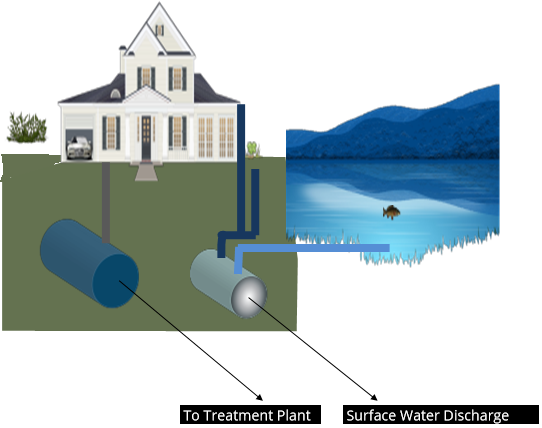
\includegraphics[scale=0.45]{SeperatedSystem1} \hspace{1 cm} 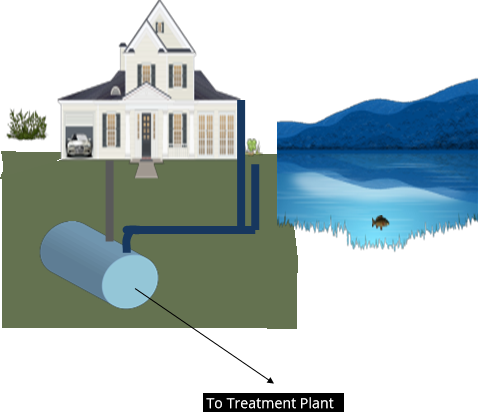
\includegraphics[scale=0.45]{CombinedSystem1}
\end{center}
			\hspace{2.6cm} Separated System \hspace{3.2cm} \parbox{\textwidth}{Combined System}\\

\section{Collections Systems Basics}\index{Collections Systems Basics}
	\begin{itemize}
\item The primary type of a collection system is a \hl{gravity system}. A gravity system is so named because the wastewater flows down gradient in the sewer, driven by forces of gravity. 
\item The collection system includes the gravity sewers, force mains, manholes, pumping equipment, and other facilities that collect and convey the water to a wastewater treatment plant. 
\item Sewers are generally laid at a minimum slope to ensure open channel flow through the pipe at a \hl{minimum velocity of 2.0 feet per second}. The minimum velocity is required to ensure that solids do not settle out in the sewer.  
\item When the sewer lines reach a certain depth, the flow must be lifted back through a lift or pump station.  
\item \hl{Lift stations} are built whenever wastewater must be pumped to a higher altitude, whether it's to lift water up so that it can gravity flow or to pump it over a rise or hill.  
\item The discharge from the pump station may be to another gravity sewer at that location or through a pressurized force main. 
\item Key elements of lift stations include a wastewater receiving well (wet-well), pumps and piping with associated valves.
\item The size of the wet well affects the operating of the station. If a wet well is too small, excessive starting and stopping of the pump motors will occur, resulting in premature failure. If the wet well is too large, solids will tend to settle on the bottom, blocking the pump suction line and leading to the generation of hydrogen sulfide and methane.
\item The dry well is the portion of the dry well/wet well pumping station that houses the necessary equipment required to pump the wastewater. The dry well is so named because it is isolated from the incoming wastewater.
\item Centrifugal pumps are the most common type of pump found in wastewater pumping stations. 
\item In the USA, wastewater generated in a typical home is about 70 gal/day/person
\end{itemize}

\section{Collections Related Operational Issues}\index{Collections Related Operational Issues}
Infiltration and inflow (I/I) is the unwanted flow into the wastewater collections systems.
\subsection{Infiltration}\index{Infiltration}
\begin{itemize} 
\item Groundwater entering sanitary sewers through defective pipe joints and broken pipes is called infiltration. \hl{Remember:  \textbf{ground filters}}
\end{itemize}

\subsection{Inflow}\index{Inflow}
\begin{itemize} 
\item During rainstorms or snow thaws, large volumes of water may flow into the wastewater collections systems through leaky manhole covers or combined storm-water /wastewater connections.  In addition, private residences may have roof, cellar, yard, area, or foundation drains inappropriately connected to sanitary sewers.  These flows are termed as inflows. \hl{Remember: \textbf{rain flow}}
\end{itemize}

\textbf{Implications of I/I:}\\%$$$$$$$$$$$$$$$$$$$$%
\begin{itemize}
\item I/I decrease the efficiency and capacity of wastewater collection systems and treatment systems 
\item I/I can advance the need for capital costs to manage and treat flows
\item I/I contribute to the hydraulic overloading of treatment processes, which can affect public health and the compliance with NPDES permit requirements
\item I/I could cause Sanitary and combined sewer overflows(SSOs and CSOs) when wastewater flow volumes exceed the design capacity of the treatment plant 
\item I/I increase collection system and treatment facility operating costs
\end{itemize}

\subsection{Odors}\index{Odors}
\begin{itemize}
\item Hydrogen sulfide (H$_2$S), its associated compounds and methane are generated due to microbial

 activity in wastewater and the conveyance systems.  The \hl{rotten egg like smell} of hydrogen sulfide causes public nuisance odors, poses a health hazard for collections systems workers and causes corrosion of the system through its conversion to sulfuric acid.  The hydrogen sulfide generation is typically controlled by reducing the potential for septicity in wastewater through proper design of the system -  adequate velocities and adequate air space and through chemical treatment.
 \end{itemize}

\subsection{Fats, Oils and Grease (FOG)}\index{Fats, Oils and Grease (FOG)}
\begin{itemize}
\item FOG from food home, food establishments and industries affect the operation of the collection system
\item FOG has a tendency to accumulate in sewer pipes decreasing its wastewater carrying capacity.
\item Excessive FOG accumulation may cause sewer overflows
 \end{itemize}


%% \documentclass{article}
% %\usepackage[english]{babel}%
% \usepackage{graphicx}
% \usepackage{tabulary}
% \usepackage{tabularx}
% \usepackage[normalem]{ulem}
% \usepackage{cancel}
% \usepackage{tikz} 
% \usepackage{pdflscape}
% \usepackage{colortbl}
% \usepackage{lastpage}
% \usepackage{multirow}
% \usepackage{enumerate}
% \usepackage[shortlabels]{enumitem}
% \usepackage{color,soul}
% \usepackage{pdflscape}
% \usepackage{hyperref}
% %\usepackage[table]{xcolor}
% \usepackage{rotating}
% \usepackage{amsmath}
% \usepackage{fixltx2e}
% \usepackage{framed}
% \usepackage{mdframed}
% \usepackage[T1]{fontenc}
% \usepackage[utf8]{inputenc}
% \usepackage{textcomp}
% \usepackage{siunitx}
% \usepackage{ifthen}
% \usepackage{fancyhdr}
% \usepackage{gensymb}
% \usepackage{newunicodechar}
% \usepackage[document]{ragged2e}
% \usepackage[margin=1in,top=1.1in,headheight=57pt,headsep=0.1in]
% {geometry}
% \usepackage{ifthen}
% \usepackage{fancyhdr}
% \everymath{\displaystyle}
% \usepackage[document]{ragged2e}
% \usepackage{fancyhdr}
% \everymath{\displaystyle}
% \usepackage{empheq}

% \usepackage[most]{tcolorbox}

% \usepackage{booktabs} % Required for nicer horizontal rules in tables


% \usepackage{enumitem}

% %\usepackage[table,xcdraw]{xcolor}
% \usetikzlibrary{arrows}
% \linespread{2}%controls the spacing between lines. Bigger fractions means crowded lines%
% %\pagestyle{fancy}
% %\usepackage[margin=1 in, top=1in, includefoot]{geometry}
% %\everymath{\displaystyle}
% \linespread{1.3}%controls the spacing between lines. Bigger fractions means crowded lines%
% %\pagestyle{fancy}
% \pagestyle{fancy}
% \setlength{\headheight}{56.2pt}

% \definecolor{myblue}{rgb}{.8, .8, 1}
% \newcommand*\mybluebox[1]{%
% \colorbox{myblue}{\hspace{1em}#1\hspace{1em}}}

% \chead{\ifthenelse{\value{page}=1}{
\includegraphics[scale=0.3]{SCC}\\ \textbf \textbf Wastewater Constituents Analysis \& Laboratory Methods}}
% \rhead{\ifthenelse{\value{page}=1}{}{}}
% \lhead{\ifthenelse{\value{page}=1}{}{Wastewater Constituents Analysis \& Laboratory Methods}}
% \rfoot{\ifthenelse{\value{page}=1}{Module 1: WATR 048 - Spring 2019}{Module 1: WATR 048 - Spring 2019}}

% \lfoot{Shabbir Basrai}
% \cfoot{Page \thepage\ of \pageref{LastPage}}
% \renewcommand{\headrulewidth}{2pt}
% \renewcommand{\footrulewidth}{1pt}
% \begin{document}
% %\begin{empheq}[box=\mybluebox]{align}
% %a&=b\\
% %E&=mc^2 + \int_a^a x\, dx
% %\end{empheq}

% \newlist{steps}{enumerate}{1} % Defines "Steps" for enumerate as Step 1, Step 2 etc.
% \setlist[steps, 1]{label = Step \arabic*:} % Defines "Steps" for enumerate as Step 1, Step 2 etc.

% \setlist{nolistsep} % Reduce spacing between bullet points and numbered lists


%_______________________________________________________________________________________________________________________________________%
\chapterimage{Preliminary.jpg} % Chapter heading image

\chapter{Preliminary Treatment}
% \begin{enumerate}[1.]
% 	\definecolor{shadecolor}{RGB}{200, 200, 240}

% 	%%%%%%%%%%%
% 	% LEVEL 2 %
% 	%%%%%%%%%%%

% 	\begin{snugshade*}
% 		\item \noindent\textsc{Wastewater Constituents}%$$$$$$$$$$$$$$$$$$$$%
% 	\end{snugshade*}
% 	Solids, organic matter, nutrients, pathogens and oil \& grease are the main target constituents of wastewater treatment operations.
% 	\begin{enumerate}[A.]%___________%
% 			\definecolor{shadecolor}{RGB}{225, 235, 235}

				%%%%%%%%%%%
				% LEVEL 3 %
				%%%%%%%%%%%
		% \begin{snugshade*}
		% 	\item \noindent\textsc{Organic Matter}%###############################%
		% \end{snugshade*}






			\begin{itemize}
				\item The objective of preliminary treatment is to remove coarse solids and other large materials often found in raw wastewater
				\item Removal of these materials is necessary to enhance the operation and maintenance of subsequent treatment units\\
				\item Preliminary treatment operations typically include a combination of the following processes:
					\begin{itemize}
						\item Screening
						\item Grinding or shredding
						\item Flow measurement
						\item Grit removal
						\item Pre-aeration
						\item Flow equalization
					\end{itemize}
			\end{itemize}

				
		\section{Process Elements of Preliminary Treatment}\index{Process Elements of Preliminary Treatment}	
			
		\subsection{Screening}\index{Screening}
					\begin{itemize}
						\item Screening is typically the first unit in a preliminary treatment
						\item Screening allows for the capture of coarse solids as pieces of cloths garbage so as to protect pumps and other units from clogging. 
						\item Screens may consist of vertical or inclined bars (bar racks or bar screens), wire mesh or perforated plates having either circular or rectangular openings. 
						\item Screens remove the large, entrained, suspended or floating solids such as pieces of wood, cloth, paper, plastics, garbage, etc.
						\item Debris collected on the screen can be cleaned manually or automatically using chain driven rakes 
						\item The retained material at screens - screenings, is collected and hauled to landfill for disposal
						\item The quantity of screenings removed varies by location and is a function of the clear opening of the screen.
						\item Barmuinitors combine the function of a screen and a grinder.  The ground material is returned to the wastewater flow for removal during primary treatment.
					\end{itemize}

\begin{figure}
\begin{center}
    \includegraphics[width=0.7\linewidth]{Barscreen}\\

Barscreen - No rakes
\end{center}
  \end{figure}
  
 \begin{center}
    \includegraphics[scale=0.6]{Blank}\\
\hspace{0cm} Video: Automatic Barscreen
  \end{center}
 
		\subsection{Grinding and Shredding}\index{Grinding and Shredding}

					\begin{itemize}
\begin{minipage}{\textwidth}	\item Comminutor(Grinder) consist of fixed, rotating or oscillating teeth or blades, acting together to reduce the solids to a size which will pass through fixed or rotating screens grind rags into small chunks
\item The comminutors are installed in wastewater channel and they grind the larger solids without actually removing them from the wastewater.  These devices may be installed before the screens or as a combination of screen and cutters (barmunitors).
					\end{minipage}	
					\end{itemize}
					\begin{minipage}{\textwidth}
					\begin{center}
      \includegraphics[width=0.3\linewidth, height=70mm]{Comminutor}\\
      Comminutor\\
\end{center}
    \end{minipage}

\begin{figure}[h]
    \includegraphics[width=\linewidth]{Comminutor1}\\
    \hspace{5cm}Schematic of comminutor placement in a channel\\
%    \caption{Comminutor Schematic}
  \end{figure}
  
		\subsection{Flow Measurement}\index{Flow Measurement}
					\begin{itemize}
						\item Wastewater flow to a treatment plant is not constant but varies in a diurnal (daily) pattern reflecting domestic water use activity.
						\item Continuous flow measurement is necessary in order to monitor diurnal variations in flow which may affect treatment plant efficiency.\\
						\item Devices used for flow measurement as part of the preliminary treatment can be placed in a channel or in a pipe.
					\end{itemize}

		\subsubsection{Devices for Flow Measurement in Channels}\index{Devices for Flow Measurement in Channels}

					\begin{itemize}
						\item Weirs: 
							\begin{itemize}
								\item Typically sharp crested weirs which are essentially metal plates installed perpendicular the flow.  The plate may a straight edge, a V-notch, or a trapezoidal opening.
								\item The weir plate in the channel causes an increase in the depth of the water behind the weir.  which is proportional to the flow rate.
								\item The flow rate can be determined by calculation or by reading the corresponding flow value to the depth of the water, from a chart specific for that weir. 
								
						
\begin{figure}[h!]
  \centering
  \begin{subfigure}[b]{0.4\linewidth}
    \includegraphics[width=\linewidth]{ChannelWeir}
    \caption{Weir in a channel}
  \end{subfigure}
  \hspace{1cm}
  \begin{subfigure}[b]{0.4\linewidth}
    \includegraphics[width=\linewidth]{WierTypes}
    \caption{Weir types}
  \end{subfigure}
\end{figure}
								
								
								
							\end{itemize}
						\item Parshall Flume:
							\begin{itemize}
								\item Parshall flume uses a narrow section in the channel as the restriction rather than the vertical plate of a weir.
								\item Like the weir, the restriction due to the narrow section of the flume, causes an increase in the depth of the water behind the weir (head) which is proportional to the flow rate.
								\item The flow rate can be determined by calculation or by reading the corresponding flow value to the depth of the water, from a chart specific for that Parshall Flume. 
								\end{itemize}

					\end{itemize}
\begin{figure}[h!]
  \centering
  \begin{subfigure}[b]{0.4\linewidth}
    \includegraphics[width=0.75\linewidth]{parshallflume1}
    \caption{Parshall flume}
  \end{subfigure}
  \hspace{1cm}
  \begin{subfigure}[b]{0.4\linewidth}
    \includegraphics[width=\linewidth]{parshallflume2}
    \caption{Parshall flume with level sensor}
  \end{subfigure}
\end{figure}
		\subsubsection{Devices for Flow Measurement in Pipes}\index{Devices for Flow Measurement in Pipes}
					
					\begin{itemize}
						\item Venturi Tube:
							\begin{itemize}
								\item Measures the difference in pressure in the inlet and center section (throat)
								\item This pressure difference can then be mathematically converted to a flow rate.
								\item Works only when a pipe if flowing full
							\end{itemize}
						\item Magnetic Flow Meter (Magmeter):
							\begin{itemize}
								\item Magmeter is a pipe spool which has an electromagnetic coil surrounding it.  As the wastewater - a conducting material, flows through it, an electrical current is created proportional to the velocity of the conducting fluid (wastewater).
								\item Flow is automatically calculated by multiplying the velocity by the cross- sectional area of the pipe.
								\item Similar to the venturi meter, magmeter will read accurately only if the magmeter section of the pipe is flowing full and the wastewater is flowing through it at a certain minimum velocity.
							\end{itemize}
\begin{figure}[h!]
  \centering
  \begin{subfigure}[b]{0.4\linewidth}
    \includegraphics[width=0.9\linewidth]{magmeter1}
    \caption{Magmeter}
  \end{subfigure}
  \hspace{1cm}
  \begin{subfigure}[b]{0.45\linewidth}
    \includegraphics[width=\linewidth]{magmeter}
    \caption{Piping with magmeters}
  \end{subfigure}
\end{figure} 
					\end{itemize}
		\subsection{Grit Removal}\index{Grit Removal}
						\begin{itemize}
							\item Grit includes sand, gravel, cinder, eggshells, bone chips, seeds, coffee grounds, and large organic particles, such as food waste.
							\item Purpose of Grit removal:
								\begin{itemize} 
									\item to protect mechanical equipment from abrasion and abnormal wear 
									\item to reduce clogging caused by deposition of grit particles in pipes and channels, and 
				\item to prevent loading the treatment plant with inert matter that might interfere with the operation of treatment units such as anaerobic digester and aeration tanks.
			\end{itemize}
		\item Removal of organic material along with the grit is undesirable for two reasons:
			\begin{enumerate}
				\item It causes odor issues, and 
				\item Organic matter is a potential source of energy (digester gas)
			\end{enumerate}
		\item Grit Disposal: Grit removed is typically landfilled.
		\item Grit Volume:  The volume of grit collected measured in ft$^3$/MG.
		\item The rate of grit collection can range from 0.5 ft$^3$/MG to 30 ft$^3$/MG.
		\item Wastewater plants having a combined collection system must deal with much larger volumes of grit.
\end{itemize}
\subsubsection{Grit Removal Systems}\index{Grit Removal Systems}



			\begin{itemize}
			
					\item \noindent\textsc{Horizontal grit chambers:}

					\begin{itemize}
						\item These are rectangular channels 30 to 60 feet long and the water detention time is between 45 to 90 seconds
						\item Water passing through these channels is maintained at a relatively constant \hl{velocity of about 1 feet per second (fps)} which allows for the grit to settle while keeping the lighter organic material to stay in suspension and continue on into the primary clarifiers.
					\end{itemize}
	

						\item \noindent\textsc{Aerated grit chambers:}
	
					\begin{itemize}
						\item The 1 fps velocity is maintained by using aerators to create a rolling flow in the tank.
						\item Aeration is achieved using diffusers located on the bottom of one side of the grit chamber.
						\item Aerated grit chambers help create aerobic conditions in septic sewage. Aerobic conditions help improve the settleability of the sludge and increase both BOD and suspended solids removal in the primary clarifiers.
						\item Much larger and deeper than non-aerated units.
						\item The detention times are increased to 3 to 5 minutes.
					\end{itemize}

\begin{figure}[h!]
  \centering
  \begin{subfigure}[b]{0.46\linewidth}
    \includegraphics[width=0.8\linewidth]{HorizontalGritChamber}
    \caption{Horizontal grit chamber}
  \end{subfigure}
  \hspace{0.2cm}
  \begin{subfigure}[b]{0.5\linewidth}
    \includegraphics[width=0.8\linewidth]{AeratedGritChamber}
    \caption{Aerated grit chamber}
  \end{subfigure}
\end{figure} 					


						\item \noindent\textsc{Cyclonic/Vortex grit chamber:}


					\begin{itemize}
						\item The wastewater flows into a cylinder that tapers to a cone at one end.
						\item The flow whirls around the inside of the cylinder like a cyclone which causes the heavy grit to be slinged to the outside and it ultimately settles to the bottom from where it is withdrawn.
					\end{itemize}

\begin{figure}[h!]
  \centering
  \begin{subfigure}[b]{0.47\linewidth}
    \includegraphics[width=0.8\linewidth]{VortexGritChamber1}
    \caption{Vortex grit chamber design}
  \end{subfigure}
  \hspace{0.2cm}
  \begin{subfigure}[b]{0.43\linewidth}
    \includegraphics[width=0.8\linewidth]{VortexGritChamber}
    \caption{Vortex grit chamber installed}
  \end{subfigure}
\end{figure} 
	
\subsubsection{Grit Removal}\index{Grit Removal}		

		
			\begin{itemize}
				\item In the cyclonic/vortex grit chamber, the grit is scoured with water and is removed using pumps
				\item For the horizontal and aerated grit systems:
					\begin{itemize}
						\item Mechanical augers at the bottom of the grit chamber move the grit to one end of the tank where grit slurry pumps can pump it out of the tank to a grit separator.
						\item In some cases steep bottom slope is provided which will collect the grit at Central Point of Removal.
						\item Grit Removal is achieved by air pumps for small aerated grit chambers.
						\item Grit can also be removed by tubular conveyors, buckets type collectors, elevators screws conveyors, grit pumps and clam shell buckets
					\end{itemize}
			\end{itemize}
						\end{itemize}
%		\end{itemize}

\subsection{Flow Control}\index{Flow Control}	
	\begin{itemize} 
		\item Flow control is critical for grit removal, specifically for the horizontal and aerated grit chambers as excessive or inadequate velocities would lead to poor grit removal or cause excessive organic material settling along with the grit, respectively
		\item As the wastewater flows vary diurnally, it is important that velocity of the wastewater in the grit chamber should be maintained nearly constant - near 1 fps.
		
\begin{figure}[h]
    \includegraphics[width=\linewidth]{DiurnalFlow}\\
\begin{center}
Diurnal wastewater flow profile \\
\end{center}
%    \caption{Comminutor Schematic}
  \end{figure}		

		\item Constant velocity in a grit chamber is achieved by providing a \hl{proportional (Sutro) weir} at the outlet end of grit chamber.
		\item The shape of the opening between the plates of a proportional weir is made in such a way that the discharge is directly proportional to liquid depth in grit chamber resulting in maintaining a constant velocity of water even a the flow changes.
	\end{itemize}
\begin{figure}[h!]
  \centering
  \begin{subfigure}[b]{0.5\linewidth}
    \includegraphics[width=0.8\linewidth]{Sutroweir1}
    \caption{Proportional weir design}
  \end{subfigure}
  \hspace{1cm}
  \begin{subfigure}[b]{0.35\linewidth}
    \includegraphics[width=0.8\linewidth]{Sutroweir}
    \caption{Installed Proportional weir}
  \end{subfigure}
\end{figure} 

\subsection{Pre-aeration}\index{Pre-aeration}	
	\begin{itemize}
		\item Pre-aeration of the wastewater as part of the preliminary treatment may be provided as a separate process or increased detention time in an aerated grit chamber.
		\item Pre-aeration provides the follwoing benefits:
			\begin{itemize}
				\item freshens up wastewater by dissolving oxygen thereby reducing the wastewater septicity
				\item reduction of septicity allows for better settling - solids and BOD removal, in the following primary treatment process
				\item promotes grease separation which facilitates its removal during primary treatment
			\end{itemize}
	\end{itemize}
\subsection{Flow Equalization}\index{Flow Equalization}	

	\begin{itemize}
		\item Flow equalization involves storing a portion of peak flows for release during low-flow periods
		\item It prevents surges and allows for the operation of processes at design flows thus allowing for optimal physical, biological and chemical processes to take place.
		\item It results in saving capital costs as the processes may be built with a treatment capacity which is less than the peak flows
	\end{itemize}

\section{Preliminary Treatment Math Problems}\index{Preliminary Treatment Math Problems}

Preliminary Treatment math problems relate to the following:

\subsection{Channel Velocity and Flow Rate}\index{Channel Velocity and Flow Rate}
Flow Rate - Q (volume/time) = velocity (distance or length traveled /time) * surface area\\
Velocity is the speed at which the water is flowing.  It is measured in units of length/time – ft./sec.\\
Velocity of water flowing through can be calculated by dividing the flow rate by area of the flow stream.\\
\vspace{0.5cm}
$Velocity \enspace \dfrac{length}{time}= \dfrac{flow \enspace rate(\dfrac{volume \enspace or \enspace cubic \enspace length}{time})}{surface \enspace area \enspace in \enspace the \enspace direction \enspace of \enspace flow-square \enspace length}$\\
\vspace{0.5cm}
\textbf{For a flow in a channel:}\\
\vspace{0.5cm}
\hl{Example Problems:}\\
\begin{enumerate}[1.]
\item Calculate the velocity of a 14 MGD flow in a 6 ft wide channel with a water depth of two feet.\\
\begin{center}
\includegraphics[scale=0.5]{ChannelFlow3}
\end{center}
$Flow (Q) = Velocity (V) * Area (A)$\\
$\implies 14 \dfrac{MG}{day}* \dfrac{10^6 gal}{MG} * \dfrac{ft^3}{7.48 gal}*\dfrac{day}{24*60*60} = V \dfrac{ft}{sec}* 6 ft * 2 ft \implies 21.7 \dfrac{ft^3}{sec}= 12V\dfrac{ft^3}{sec}$\\
$\implies V \dfrac{ft}{sec}= \dfrac{21.7}{12}= \boxed{1.8\dfrac{ft}{sec}}$\\

\item Calculate the flow, in gpd, that would pass through a grit chamber 2 feet wide, at a depth of 6 inches, with a velocity of 1 ft /sec\\
Solution:\\
\includegraphics[scale=0.5]{ChannelFlow3}\\
$Q=V*A$\\
$Q=1\dfrac{ft}{s}*(2*0.5)ft^2=1\dfrac{ft^3}{s}$\\
$Q=1\dfrac{\cancel{ft^3}}{\cancel{s}}*\dfrac{(1440*60)\cancel{s}}{day}*7.48\dfrac{gal}{\cancel{ft^3}}=\boxed{646,272\dfrac{gal}{day}}$
\vspace{0.5cm}
\item A wastewater channel is 3.25 feet wide and is conveying a wastewater flow of 3.5 MGD. The wastewater flow is 8 inches deep. Calculate the velocity of this flow.\\
Solution:\\
\includegraphics[scale=0.5]{ChannelFlow3}\\
$Q=V*A \implies V=\dfrac{Q}{A}$\\
$\implies V\dfrac{ft}{s}=\dfrac{3.5\dfrac{\cancel{MG}}{\cancel{day}}*\dfrac{1000000\cancel{gal}}{\cancel{MG}}*\dfrac{ft^{\cancel{3}}}{7.48\cancel{gal}}*\dfrac{\cancel{day}}{(1440*60)s}}{(3.25*0.75)\cancel{ft^2}}=\boxed{2.2\dfrac{ft}{s}}$
\vspace{0.5cm}
\item A plastic float is dropped into a wastewater channel and is found to travel 10 feet in 4.2 seconds. The channel is 2.4 feet wide and is flowing 1.8 feet deep. Calculate the flow rate of this wastewater in cubic feet per second.\\
Solution:\\
$Q=V*A$\\
$\implies Q\Big(\dfrac{ft^3}{s}\Big)=\dfrac{10ft}{4.2s}*(2.4*1.8)ft^2=\boxed{10.3\dfrac{ft^3}{s}}$
\end{enumerate}

\subsection{Grit Removal Rates}\index{Grit Removal Rates}
\emph{Typical grit removal ranges from 0.5 to 30 ft$^3$/MG}\\
\vspace{0.3cm}
\hl{Example Problems:}\\
\begin{enumerate}[1.]
\item At a wastewater treatment plant which receives a flow rate of 650,000 gallons per day, a total of 50 cubic feet of grit was removed for the month. Calculate the rate of grit removal assuming 30 days in a month.\\
Solution:\\
$Grit Removal\dfrac{ft^3}{MG}=50\dfrac{ft^3}{ \cancel{month}}*\dfrac{\cancel{month}}{30\cancel{days}}*\dfrac{\cancel{day}}{650,000\cancel{gal}}*1,000,000\dfrac{\cancel{gal}}{MG}=\boxed{2.6\dfrac{ft^3}{MG}}$
\end{enumerate}

%% \documentclass{article}
% %\usepackage[english]{babel}%
% \usepackage{graphicx}
% \usepackage{tabulary}
% \usepackage{tabularx}
% \usepackage[normalem]{ulem}
% \usepackage{cancel}
% \usepackage{tikz} 
% \usepackage{pdflscape}
% \usepackage{colortbl}
% \usepackage{lastpage}
% \usepackage{multirow}
% \usepackage{enumerate}
% \usepackage[shortlabels]{enumitem}
% \usepackage{color,soul}
% \usepackage{pdflscape}
% \usepackage{hyperref}
% %\usepackage[table]{xcolor}
% \usepackage{rotating}
% \usepackage{amsmath}
% \usepackage{fixltx2e}
% \usepackage{framed}
% \usepackage{mdframed}
% \usepackage[T1]{fontenc}
% \usepackage[utf8]{inputenc}
% \usepackage{textcomp}
% \usepackage{siunitx}
% \usepackage{ifthen}
% \usepackage{fancyhdr}
% \usepackage{gensymb}
% \usepackage{newunicodechar}
% \usepackage[document]{ragged2e}
% \usepackage[margin=1in,top=1.1in,headheight=57pt,headsep=0.1in]
% {geometry}
% \usepackage{ifthen}
% \usepackage{fancyhdr}
% \everymath{\displaystyle}
% \usepackage[document]{ragged2e}
% \usepackage{fancyhdr}
% \everymath{\displaystyle}
% \usepackage{empheq}

% \usepackage[most]{tcolorbox}

% \usepackage{booktabs} % Required for nicer horizontal rules in tables


% \usepackage{enumitem}

% %\usepackage[table,xcdraw]{xcolor}
% \usetikzlibrary{arrows}
% \linespread{2}%controls the spacing between lines. Bigger fractions means crowded lines%
% %\pagestyle{fancy}
% %\usepackage[margin=1 in, top=1in, includefoot]{geometry}
% %\everymath{\displaystyle}
% \linespread{1.3}%controls the spacing between lines. Bigger fractions means crowded lines%
% %\pagestyle{fancy}
% \pagestyle{fancy}
% \setlength{\headheight}{56.2pt}

% \definecolor{myblue}{rgb}{.8, .8, 1}
% \newcommand*\mybluebox[1]{%
% \colorbox{myblue}{\hspace{1em}#1\hspace{1em}}}

% \chead{\ifthenelse{\value{page}=1}{\includegraphics[scale=0.3]{SCC}\\ \textbf \textbf Wastewater Constituents Analysis \& Laboratory Methods}}
% \rhead{\ifthenelse{\value{page}=1}{}{}}
% \lhead{\ifthenelse{\value{page}=1}{}{Wastewater Constituents Analysis \& Laboratory Methods}}
% \rfoot{\ifthenelse{\value{page}=1}{Module 1: WATR 048 - Spring 2019}{Module 1: WATR 048 - Spring 2019}}

% \lfoot{Shabbir Basrai}
% \cfoot{Page \thepage\ of \pageref{LastPage}}
% \renewcommand{\headrulewidth}{2pt}
% \renewcommand{\footrulewidth}{1pt}
% \begin{document}
% %\begin{empheq}[box=\mybluebox]{align}
% %a&=b\\
% %E&=mc^2 + \int_a^a x\, dx
% %\end{empheq}

% \newlist{steps}{enumerate}{1} % Defines "Steps" for enumerate as Step 1, Step 2 etc.
% \setlist[steps, 1]{label = Step \arabic*:} % Defines "Steps" for enumerate as Step 1, Step 2 etc.

% \setlist{nolistsep} % Reduce spacing between bullet points and numbered lists


%_______________________________________________________________________________________________________________________________________%
%----------------------------------------------------------------------------------------------%
\chapterimage{Week3Clarifier1.jpg} % Chapter heading image

\chapter{Primary Treatment}

%\section{Background}\index{Background}
\begin{itemize}
\item Synonyms:  primary treatment basin, primary clarifier, sedimentation basin, primaries, clarifier

	
		\item Primary treatment is after preliminary treatment and 				before secondary treatment
		\item Its two main objectives are: 
			\begin{itemize}
				\item Remove settleable solids
				\item Remove floatable solids
			\end{itemize}
		\item This is a physical process which relies on the physical 			properties - how heavy or light the suspended solids particles 		are to effect its separation
		\item Provides quiescent conditions for the influent 					wastewater for the heavier solids to settle and the lighter 			solids to float
		\item Removes settleable solids and floatables
		\item Settled solids are removed as sludge from the bottom of 			the clarifier
		\item Floatable solids including oil and grease are also 				removed, as scum from the surface\\
		\item The shape of the primary clarifier is either rectangular 		or circular
	
		\item Effective solids removal in the primary clarifiers will 			reduce the loading on the expensive secondary treatment 				process.
		\item The amount of solids removed during primary treatment 			may be enhanced by chemical addition - ferric or ferrous 				chloride as a coagulant and anionic polymer as the flocculant.  		This is called Chemically Enhanced Primary Treatment (CEPT).
\item \textbf{Typical Removal Rates:}\\
\begin{itemize}
\item \hspace{10mm} BOD removal – 25\% to 40\% and about 60\% with CEPT
\item \hspace{10mm} Suspended solids (SS) removal – 40\% to 60\% and about 75\% with CEPT
\item \hspace{10mm} Settleable Solids removal - $>$90\%
\end{itemize}
\end{itemize}
\clearpage
			\begin{center}
				\includegraphics[scale=0.9]{RectangularClarifier}\\
				Cross section of a Rectangular Clarifier\\

				\includegraphics[scale=0.1]{Blank}\\
				\includegraphics[scale=0.6]{CircularClarifierAI}\\
				Schematic cross section of a circular clarifier\\
				\includegraphics[scale=0.1]{Blank}\\
				\includegraphics[scale=0.5]{CircularClarifier3}\\
				Cross section of a circular clarifier\\
			\end{center}
				\includegraphics[scale=0.03]{Blank}\\


\section{Clarifier Zones}\index{Clarifier Zones}
				
\subsection{Inlet Zone}\index{Inlet Zone}		
				\begin{itemize}
					\item Inlet Zone is where the water enters the end 					of a rectangular tank, or the center of a circular 					or square tank.
					\item The Inlet Zone is designed to accomplish two 					objectives:
						\begin{enumerate}
							\item Reduce the velocity (dissipate 									energy in the incoming water)
							\item Distribute the flow evenly
						\end{enumerate}
					\item The inlet zone is equipped with a baffle.  					Inlet baffle reduces the velocity of the 							influent flow, prevent short circuiting which 							could cause solids being carried over to secondary 					treatment.  
						\begin{itemize}
							\item Circular tanks are equipped with a 								collar-type circular baffle that directs 								the water down as it enters the center of 								the tank.
							\item Rectangular tanks will have a plate 								baffle in front of the opening for the 									wastewater flow into the clarifier and 									another baffle just upstream - a 										perforated wall or a picket fence type 									baffle that spreads the water laterally 								across the inlet end of the tank.\\

\begin{figure}[h!]
  \centering
  \begin{subfigure}[b]{0.4\linewidth}
    \includegraphics[width=0.8\linewidth]{InfluentBaffle}
    \caption{Rectangular clarifier influent baffle}
  \end{subfigure}
  \hspace{1cm}
  \begin{subfigure}[b]{0.4\linewidth}
    \includegraphics[width=\linewidth]{CircularClarifierInfluentBaffle}
    \caption{Circular clarifier influent baffle}
  \end{subfigure}
\end{figure}	
	
%							\begin{center}
%							\includegraphics[scale=0.65]												{InfluentBaffle}\\
%							Rectangular clarifier influent baffle
%							\end{center}
%							
%														\begin{center}
%							\includegraphics[scale=0.65]												{CircularClarifierInfluentBaffle}\\
%							Circular clarifier influent baffle
%							\end{center}	
						\end{itemize}
				\end{itemize}

\subsection{Settling Zone}\index{Settling Zone}
			\begin{itemize}
				\item This is the largest portion of the tank where 					solids settle.
				\item The water velocity is reduced to 0.03-0.05 fps 					and the detention time is about 1.5 to 2 hours. 
				\item A clarifier is said to be short circuiting if 					the velocity of the water is greater in some sections 					than in others. The water passing through the higher 					velocity region will have a reduced detention time and 				settleable solids will carry through with this water 					as it goes over the weir.  Short circuiting is 							prevented by appropriately designing inlet baffles and weir plates (at the Outlet Zone).
			\end{itemize}

\subsection{Sludge Zone}\index{Sludge Zone}
			\begin{itemize} 
				\item Sludge zone is the bottom of the tank where the 					settled sludge collects and compacts.
				\item Sludge blanket depth should be measured and 						sludge should be removed at least every shift. A 						desirable blanket depth is typically established and 					the sludge pumping rate and regimen is established to 					maintain that desired sludge blanket level.
				\item Sludge rakes push the sludge to one end or the 					center of the tank so that it can be pumped out. 
				\item The rake drive is usually equipped with a torque 				indicator. A shear pin in the drive shaft will break 					to prevent damage to the gearbox or drive shaft. 
				\item Failure to remove sludge often enough will 						result in the sludge becoming septic releasing gas 						bubbles which hinders the sludge settling and also 						result in causing odor problems.
				\item The sludge from the primary clarifiers needs to 					be stabilized prior to its disposal.  The sludge 						(solids) from the primary clarifiers are mixed with 					the solids from the secondary treatment process and 					stabilized typically using a sludge digestion process. 
			\end{itemize}
\subsection{Skimming Zone}\index{Skimming Zone}

			\begin{itemize}
				\item The skimming zone is at the surface of the tank 					for scum removal
				\item Lighter solids and greases float to the surface 					of the clarifier as scum
				\item In Circular Clarifiers:  Floating matter is 						skimmed by a skimmer arm that is supported by the 						sludge rake and rotates with it around the tank. The 					floating matter is pushed over the beach plate by the 					wipers attached to the skimmer arm and into a scum box 				attached to the tank wall.\\
				\item In Rectangular Clarifiers:  The flights act as 							skimmers when the chain brings them to the surface and 				pushes the scum towards the scum troughs.  The scum 					trough may be designed to rotate (tip) periodically 					for the scum to flow in from the water surface.\\
							
				\item The scum collected from the primary clarifiers is sent 				to the digester for treatment along with the sludge 					removed.\\ 

				\vspace{1cm}
									\begin{center}
					\includegraphics[scale=0.06]{RotatingScumTrough}\\
					Rectangular clarifier scum trough\\
									\includegraphics[scale=0.02]{Blank}\\
				\end{center}	

				\item The flights in the rectangular clarifier are supported 				at the top by two parallel rails running along the 						length of the clarifier.\\
				\item There are wear plates (strips) installed at the 						clarifer bottom and on top of the rails to prevent the 				flights from riding directly on those surfaces.  To 					reduce friction, the flights have a wearing shoe 						attached.  
				\item Both the wear strip and the wearing shoe 					are disposable items and are replaced at fixed 							intervals.\\			
				\begin{center}
					\includegraphics[scale=0.07]												{RectangularClarifierComponents}\\
					Rectangular clarifier flights\\
				\end{center}						  
\end{itemize}
\subsection{Outlet Zone}\index{Outlet Zone}
			\begin{itemize}
				\item  This is the part of the clarifier where the 						settled water leaves to go to the secondary treatment 					processes.
				\item A channel called the effluent launder collects 					the effluent flow and directs it to the primary 						effluent piping. 
				\item Weirs are installed along the edge of the effluent launder channel to skim the water evenly off the surface of the tank. The most common type of effluent weir is a V-notch (or saw-tooth) weir.   A V-	notch weir is a plate that has notches, about 2-3 						inches deep, cut in it every 6-8 inches. If the weir is clean and level, it will remove water evenly all 					the way around the edge of the tank. This minimizes 					the upward velocities near the effluent launder and 					improves removal efficiencies. If the weir plate is not level or part of the weir becomes clogged with 				slime or debris, short-circuiting will result because 					more water will pass over the low side or the clean notches of the weir. Short-circuiting will cause poor 					settling and uneven sludge blanket buildup.
				\item In rectangular tanks the water leaves at the end 	opposite the influent.
												  
				\item In circular  tanks the water leaves at the edge of the tank.
				\item Also, in the circular clarifiers, an effluent baffle, just upstream of the weir, 					is installed to prevent floating solids from going 						over the weir.
\clearpage
				\begin{center}
					\includegraphics[scale=0.04]												{CircularClarifierComponents1}\\
					Circular clarifier skimmer arm, effluent baffle and v-notch weir\\
				\end{center}
				
			\vspace{0.8cm}
					\begin{center}
					\includegraphics[scale=0.07]												{RectangularClarifierWeir}\\
					Rectangular clarifier v-notch weir and launder\\
				\end{center}			
												  
			\end{itemize}

\clearpage
\section{Sludge Pumping}\index{Sludge Pumping}

	\begin{itemize}
		\item The sludge pumping from the clarifier must be adequate 			to prevent sludge from going septic. Septic sludges are much 			more difficult to thicken or de-water and cause odor issues. 
		\item Primary sludge normally averages 4-6\% solids. 
		Generally positive displacement pumps are used for primary 				sludge
		\item The pumping cycles must be designed to provide the 				thickest sludge possible.
		\item Excessive pumping or pumping without building solids to 			build up leads to pumping thinner (more water) sludge.
	\end{itemize}
\section{Design Parameters}\index{Design Parameters}
	\begin{itemize}
	\setlength\itemsep{1em}
		\item \textbf{Clarifier depth} – 8 to 12 feet
		\item \textbf{Hydraulic or surface loading}
			\begin{itemize}
			\item This rate is important to ensure good settleable 					solids removal efficiency
			\item It is expressed in terms of gallons per day per 					square foot (gpd/sq ft) of tank surface area
			\item Typical surface loading rate used for the design of 				primary clarifiers range between 300 to 1,400 gpd/sq ft, 				depending on the nature of the solids and the treatment 				requirements. Lower loading rates are frequently used in 				small plants in cold climates. In warm regions, low rates 				may cause excessive detention which could lead to 						septicity.
			\end{itemize}
	\end{itemize}
	
\section{Advance primary treatment (APT)}\index{Advance primary treatment (APT)}
Synonyms:  Advance primary treatment (APT), Chemically enhanced primary treatment (CEPT), Physical-chemical treatment (Phys-chem)
\subsection{Background}\index{Background}     
      
        \begin{itemize}
			\item Suspended solids present in wastewater are typically coated with bacterial slime and biological metabolic products which are negatively charged.  A significant portion of the suspended solids in wastewater do not settle easily due to gravity as:
				\begin{enumerate}
					\item the biological mass and the associated byproduct gases produced makes these particles buoyant, 
					\item the negative electrostatic charges on these particles cause these particles to be in constant state of motion due to electrostatic repulsion
				\end{enumerate}
			\item Advance primary treatment (APT) also known as Chemically enhanced primary treatment (CEPT) or Physical-chemical treatment (Phys-chem), involves chemical addition to the primary influent flow to enhance primary treatment TSS and BOD removal efficiencies
			\item a normal primary treatment process typically removes 40 to 60\% TSS and 25 to 40\% BOD.  TSS and BOD removal efficiencies of over 80\% and 60\% respectively, may be achieved by the use of APT.
			\item additional cost incurred for the chemical addition is in most cases is offsetted by the benefits which include:
				\begin{enumerate}
					\item by removing more BOD in the primary treatment cost associated with secondary treatment is reduced
					\item primary BOD is more easy to digest than the secondary biomass thus the digester gas production is increased and digested solids production is lowered thus saving biosolids hauling cost
					\item residual ferric chloride in the primary sludge provides H$_2$S and struvite control in the solids treatment processes  
				\end{enumerate}
		\end{itemize}
\vspace{0.4 cm}

\subsection{Process/mechanism}\index{Process/mechanism}    

APT is a two step chemical process:

\textbf{Coagulation}
				                \begin{itemize}
									\item Coagulation is the process by which the negative charge on these particles is reduced lowering the repulsion forces, by the use of a chemical such as ferric chloride and alum.\\
									\item The concentration of the coagulant required is dependent on the strength of the wastewater and the conveyance time of the wastewater.
									\item Typically the coagulant is added immediately after the grit chambers so the conveyance from the grit chambers to the primary clarifier provides adequate contact time and mixing.\\
									\item Parameters to ensure optimal coagulation are:
										\begin{itemize}
											\item Appropriate coagulation concentration
											\item Adequate mixing energy, and
											\item Adequate contact time
										\end{itemize}
									\item Overdosing the coagulant will adversely effect the settleability.
									\item Typical ferric chloride dosage for coagulation range from 12 to 22 mg/l.
								\end{itemize}
\textbf{Flocculation}
			                	\begin{itemize}
									\item Flocculation uses an anionic polymer - polymer which has negatively charged groups, to bridge the coagulated particles to a size which will settle in the primary clarifier.  
									\item The flocculated particles are prone to shearing thus the polymer is gently folded in with the coagulated wastewater just prior to entry into the primary clarifier
								\end{itemize}
					

\vspace{0.6cm}
\hspace{6.8 cm} \textbf{CEPT Schematic}\\
\vspace{0.6cm}
\hspace{1.5 cm}\includegraphics[scale=.13]{CEPTInitial} \hspace{0.7 cm}\includegraphics[scale=.13]{CEPTCoagulation}\hspace{0.7 cm}
\includegraphics[scale=.13]{CEPTFlocculation}\\
\hspace{0.8 cm} \textbf{Untreated Primary Inluent}\hspace{1.6 cm}\textbf{Coagulation}\hspace{2.8 cm}\textbf{Flocculation}\\	
	
	
	
	
	
\section{Math Problems}\index{Math Problems}

Types of Math Problems Related to Primary Sedimentation 

%\item Finding the clarifier hydraulic or surface loading rate
%\item Finding the clarifier detention time
%\item Finding the clarifier weir overflow rate
%\item Finding the clarifier removal efficiency
%\item Solids removal calculations
%\end{enumerate}
%\begin{enumerate}

\subsection{Hydraulic or Surface Loading Rate}\index{Hydraulic or Surface Loading Rate}

The hydraulic or surface loading rate measures how rapidly wastewater moves through the primary clarifier.  It is measured in terms of the number of gallons flowing each day through one square foot surface area of the clarifier. 
$$Clarifier \enspace hydraulic \enspace loading \enspace 	\Big(\dfrac{gpd}{ft^2}\Big) =\dfrac{Clarifier \enspace influent 	\enspace flow (gpd)}{Clarifier \enspace surface \enspace area 	(ft^2)}$$ 
		Rectangular clarifier surface area  = width * length\\
		Circular clarifier surface area  = 0.785 * Diameter$^2 $\\
\subsection{Detention Time}\index{Detention Time}

Detention time is the length of time that wastewater stays in the settling tank is called the detention time.  It is also the time it takes for a unit volume of wastewater to pass entirely through a primary clarifier\\
$$Clarifier \enspace detention \enspace time \enspace (hr) = 	\dfrac{ Clarifier \enspace volume (cu.ft \enspace or \enspace gal)}{Influent \enspace flow \enspace (cu.ft \enspace or \enspace gal)/hr)}$$
Rectangular clarifier volume = width * length * depth of water\\
Circular clarifier volume = 0.785 * Diameter$^2$ * depth of water\\
Typically volume is calculated in cu. ft and influent flow is given in gallons.  Use 7.48 gal/ft$^3$ conversion factor to convert volume in cu. ft to gallons.\\

\subsection{Weir Overflow Rate}\index{Weir Overflow Rate}
The weirs at the end of the primary clarifier allow for the even distribution of the the outlet flow across the entire length of the weir.  An adequate length of weir is needed to ensure smooth and even flow of wastewater over the weirs.  Weir overflow rate measures the number of gallons of wastewater per day flowing over one foot of weir. 

		$$Weir \enspace over \enspace flow \enspace rate \Big(\dfrac{gpd}{ft}\Big) =\Big(\dfrac{Clarifier \enspace influent \enspace  flow (gpd)}{Total \enspace effluent 					\enspace weir \enspace length \enspace (ft)}\Big)$$
		Circular clarifier weir length = 3.14 * Diameter\\

\hl{Example problem for (a), (b) and (c) above:}\\
		\vspace{0.2cm}
A circular clarifier receives a flow of 11 MGD.  If the clarifier is 90 ft. in diameter and is 12 ft. deep, what is: a) the hydraulic/surface loading rate, b) clarifier detention time in hours, and c) weir overflow rate?\\
		\vspace{0.2cm}
a) Hydraulic/surface loading rate:\\
$Clarifier \enspace hydraulic \enspace loading \enspace 	\Big(\dfrac{gpd}{ft^2}\Big) ==\dfrac{\dfrac{11\cancel{MG}}{{day}}*\dfrac{10^6gal}{\cancel{MG}}}{0.785*90^2 ft^2}=\boxed{1,730gpd/ft^2}$\\
		\vspace{0.5cm}
b) Clarifier detention time:\\
$Clarifier \enspace detention \enspace time \enspace (hr) = 	\dfrac{ Clarifier \enspace volume (cu.ft \enspace or \enspace gal)}{Influent \enspace flow \enspace (cu.ft \enspace or \enspace gal)/hr)}$\\
		\vspace{0.2cm}
$Clarifier \enspace detention \enspace time \enspace (hr) = 	\dfrac{(0.785*90^2*12)\cancel{ft^3}}{\dfrac{11\cancel{MG}}{\cancel{day}}*\dfrac{10^6\cancel{gal}}{\cancel{MG}}*\dfrac{\cancel{ft^3}}{7.48\cancel{gal}}*\dfrac{\cancel{day}}{24hrs}}=\boxed{1.2hrs}$\\
		\vspace{0.5cm}
c) Weir overflow rate:\\
		\vspace{0.2cm} 
$Weir \enspace overflow \enspace rate \Big(\dfrac{gpd}{ft}\Big) =\dfrac{\dfrac{11\cancel{MG}}{{day}}*\dfrac{10^6gal}{\cancel{MG}}}{3.14*90 ft}=\boxed{38,924gpd/ft}$\\

\subsection{Removal Efficiency}\index{Removal Efficiency}		
Primary sedimentation removes suspended wastewater solids which includes BOD.  The efficiency of the primary is established as the percentage of the amount of parameter removed.  The parameter may quantified as mass (lbs) or as concentration (mg/l).

$$Removal \enspace efficiency (\%) = \dfrac{Parameter  \enspace In - Parameter  \enspace Out}{Parameter \enspace In} * 100$$

For TSS removal:\\
$$TSS \enspace Removal \enspace efficiency (\%) = \dfrac{TSS  _{In} \enspace(mg/l)  - TSS_{Out} \enspace(mg/l)  }{TSS _{In} \enspace(mg/l)  } * 100$$

For BOD removal:\\
$$BOD \enspace Removal \enspace efficiency (\%) = \dfrac{BOD_{In} \enspace(mg/l)  - BOD_{Out} \enspace(mg/l)  }{BOD _{In} \enspace(mg/l)  } * 100$$
\subsection{Solids Removal}\index{Solids Removal}	

\hl{\textbf{Type 1 Problems:}  These involve calculating lbs of solids removed given any two of the following TSS parameters - inlet concentration, outlet concentration and removal efficiency.}\\
a. If the inlet and outlet concentrations are given, calculate the mg/l of TSS removed using: 
$$TSS_{removed} = TSS_{in}(mg/l) - TSS_{out} (mg/l) $$
Then knowing the flow, use the lbs formula to calculate the lbs solids removed.

b. If either inlet or outlet concentration is given along with the clarifier removal efficiency, using the removal efficiency calculate the unknown outlet concentration (if only the inlet is given) or the inlet concentration (if only the outlet is given)\\
i) If inlet and removal efficiency is given, calculate the outlet by subtracting the product of inlet and removal efficiency from the inlet.
$$TSS_{out}=TSS_{in} - (TSS_{in}*\%Removal)$$
Example if the removal efficiency is 60\% and the inlet concentration is 300mg/l: $$TSS_{out}=300 - 300*0.6=120mg/l$$
ii) If outlet and removal efficiency is given, calculate the inlet concentration by dividing the outlet by (1-removal efficiency).\\
$$TSS_{in}=\dfrac{TSS_{out}}{1-\%Removal}$$
Example if the removal efficiency is 60\% and the outlet concentration is 120mg/l: $$TSS_{in}=\dfrac{120}{1-0.6}=300mg/l$$ 

Note:  You may derive the above formulas by algebraically manipulating: $\%Removal=\dfrac{TSS_{in} -TSS_{out}}{TSS_{in}}$\\
\hl{Example Problem:}\\
How many lbs of solids are removed daily by a primary clarifier treating a 6 MGD flow if the average influent TSS concentration is 300 mg/l and the clarifier TSS removal efficiency is 67\%.\\
$TSS_{out}=(300mg/l - 300*0.67)=99mg/l$\\
$lbs \enspace solids \enspace  removed = (300-99)mg/l*8.34*6MGD=\boxed{10,058 \enspace lbs \enspace solids \enspace removed \enspace per \enspace day}$\\
\vspace{0.5cm}
\hl{\textbf{Type 2 Problems:}  These involve calculating the amount of sludge pumping given the solids removed.  The solids removed from the primary clarifier is sludge with a typical solids concentration of about 3\% to 5\%.}\\
Given the amount of total solids removed and given the sludge concentration, the volume of sludge pumping can be calculated as follows:  $$\dfrac{ft^3\enspace sludge\enspace pumped}{ day}= \dfrac{lbs \enspace solids \enspace (removed)}{day} * \dfrac{1 \enspace lb \enspace sludge}{(\%)\enspace lbs \enspace solids}*\dfrac{gal \enspace sludge}{8.34lb \enspace sludge}*\dfrac{ft^3 \enspace sludge}{7.48 \enspace gal} $$
So for the solids removed in the above example, if the primary sludge has 5\% solids, the required sludge pumping can be calculated as:
$$\dfrac{ft^3\enspace sludge}{day}= \dfrac{10,058 \enspace \cancel{lbs \enspace solids}}{day} * \dfrac{1 \enspace \cancel{lb \enspace sludge}}{0.05\enspace \cancel{lbs \enspace solids}}*\dfrac{\cancel{gal \enspace sludge}}{8.34\cancel{lb \enspace sludge}}*\dfrac{ft^3 \enspace sludge}{7.48 \enspace \cancel{gal}}=\boxed{3,224\dfrac{ft^3 \enspace sludge}{day}} $$

%% \documentclass{article}
% %\usepackage[english]{babel}%
% \usepackage{graphicx}
% \usepackage{tabulary}
% \usepackage{tabularx}
% \usepackage[normalem]{ulem}
% \usepackage{cancel}
% \usepackage{tikz} 
% \usepackage{pdflscape}
% \usepackage{colortbl}
% \usepackage{lastpage}
% \usepackage{multirow}
% \usepackage{enumerate}
% \usepackage[shortlabels]{enumitem}
% \usepackage{color,soul}
% \usepackage{pdflscape}
% \usepackage{hyperref}
% %\usepackage[table]{xcolor}
% \usepackage{rotating}
% \usepackage{amsmath}
% \usepackage{fixltx2e}
% \usepackage{framed}
% \usepackage{mdframed}
% \usepackage[T1]{fontenc}
% \usepackage[utf8]{inputenc}
% \usepackage{textcomp}
% \usepackage{siunitx}
% \usepackage{ifthen}
% \usepackage{fancyhdr}
% \usepackage{gensymb}
% \usepackage{newunicodechar}
% \usepackage[document]{ragged2e}
% \usepackage[margin=1in,top=1.1in,headheight=57pt,headsep=0.1in]
% {geometry}
% \usepackage{ifthen}
% \usepackage{fancyhdr}
% \everymath{\displaystyle}
% \usepackage[document]{ragged2e}
% \usepackage{fancyhdr}
% \everymath{\displaystyle}
% \usepackage{empheq}

% \usepackage[most]{tcolorbox}

% \usepackage{booktabs} % Required for nicer horizontal rules in tables


% \usepackage{enumitem}

% %\usepackage[table,xcdraw]{xcolor}
% \usetikzlibrary{arrows}
% \linespread{2}%controls the spacing between lines. Bigger fractions means crowded lines%
% %\pagestyle{fancy}
% %\usepackage[margin=1 in, top=1in, includefoot]{geometry}
% %\everymath{\displaystyle}
% \linespread{1.3}%controls the spacing between lines. Bigger fractions means crowded lines%
% %\pagestyle{fancy}
% \pagestyle{fancy}
% \setlength{\headheight}{56.2pt}

% \definecolor{myblue}{rgb}{.8, .8, 1}
% \newcommand*\mybluebox[1]{%
% \colorbox{myblue}{\hspace{1em}#1\hspace{1em}}}

% \chead{\ifthenelse{\value{page}=1}{\includegraphics[scale=0.3]{SCC}\\ \textbf \textbf Wastewater Constituents Analysis \& Laboratory Methods}}
% \rhead{\ifthenelse{\value{page}=1}{}{}}
% \lhead{\ifthenelse{\value{page}=1}{}{Wastewater Constituents Analysis \& Laboratory Methods}}
% \rfoot{\ifthenelse{\value{page}=1}{Module 1: WATR 048 - Spring 2019}{Module 1: WATR 048 - Spring 2019}}

% \lfoot{Shabbir Basrai}
% \cfoot{Page \thepage\ of \pageref{LastPage}}
% \renewcommand{\headrulewidth}{2pt}
% \renewcommand{\footrulewidth}{1pt}
% \begin{document}
% %\begin{empheq}[box=\mybluebox]{align}
% %a&=b\\
% %E&=mc^2 + \int_a^a x\, dx
% %\end{empheq}

% \newlist{steps}{enumerate}{1} % Defines "Steps" for enumerate as Step 1, Step 2 etc.
% \setlist[steps, 1]{label = Step \arabic*:} % Defines "Steps" for enumerate as Step 1, Step 2 etc.

% \setlist{nolistsep} % Reduce spacing between bullet points and numbered lists


%_______________________________________________________________________________________________________________________________________%
\chapterimage{IntroductionSecondaryTreatmentImage.jpg} % Chapter heading image

\chapter{Introduction to Secondary Treatment}
\begin{itemize}
\item While preliminary and primary treatment processes are designed primarily to remove solids from wastewater, secondary treatment is for the removal of organics.
\item Secondary treatment involves:
\begin{itemize}
\item biological conversion of the dissolved and suspended organics in wastewater into biomass, and
\item physical settling (separation) process where the solids including the biomass formed during secondary treatment is separated and removed from the treated wastewater.
\end{itemize}

\item With the removal of gross solids in the preliminary treatment followed by removable of settleable solids in the primary clarifiers and the removal of dissolved and suspended organics in the secondary treatment processes, the wastewater is considered treated.
\item Secondary treated wastewater is typically disposed or treated further for reuse or disposal (depending upon the end use/application and the NPDES permit stipulations).
\item The solids (biomass) removed from the secondary treatment is typically mixed with the solids from primary treatment and stabilized using a solids treatment process like sludge digestion prior to its disposal.
\end{itemize}
\vspace{1cm}

\textbf{Secondary treatment process incorporates one of the following three approaches:}


\section{Fixed film system}\index{Fixed Film System}	

\begin{itemize}
\item Here the microorganisms responsible for the treatment, grow on substrates such
as rocks, sand or plastic.
\item When the wastewater is spread over the substrate, the microorganisms up-take the organics present in the wastewater
\item Example of this secondary treatment process include trickling filters and rotating biological contactors\\
\end{itemize}

\section{Suspended Growth System}\index{Suspended Growth System}
\begin{itemize}
\item In this type of secondary treatment, the microbes are suspended in the
wastewater flow being treated. 
\item Air or oxygen is supplied to maintain an aerobic environment and to keep the microorganisms in suspension. 
\item Example of this secondary treatment approach include the activated sludge treatment process 
\end{itemize}

\section{Pond System}\index{Pond System}
Similar to the suspended growth, stabilization ponds are large man made bodies of water which treat wastewater using mainly natural processes including sunlight, algae and microorganisms.


%% \documentclass{article}
% %\usepackage[english]{babel}%
% \usepackage{graphicx}
% \usepackage{tabulary}
% \usepackage{tabularx}
% \usepackage[normalem]{ulem}
% \usepackage{cancel}
% \usepackage{tikz} 
% \usepackage{pdflscape}
% \usepackage{colortbl}
% \usepackage{lastpage}
% \usepackage{multirow}
% \usepackage{enumerate}
% \usepackage[shortlabels]{enumitem}
% \usepackage{color,soul}
% \usepackage{pdflscape}
% \usepackage{hyperref}
% %\usepackage[table]{xcolor}
% \usepackage{rotating}
% \usepackage{amsmath}
% \usepackage{fixltx2e}
% \usepackage{framed}
% \usepackage{mdframed}
% \usepackage[T1]{fontenc}
% \usepackage[utf8]{inputenc}
% \usepackage{textcomp}
% \usepackage{siunitx}
% \usepackage{ifthen}
% \usepackage{fancyhdr}
% \usepackage{gensymb}
% \usepackage{newunicodechar}
% \usepackage[document]{ragged2e}
% \usepackage[margin=1in,top=1.1in,headheight=57pt,headsep=0.1in]
% {geometry}
% \usepackage{ifthen}
% \usepackage{fancyhdr}
% \everymath{\displaystyle}
% \usepackage[document]{ragged2e}
% \usepackage{fancyhdr}
% \everymath{\displaystyle}
% \usepackage{empheq}

% \usepackage[most]{tcolorbox}

% \usepackage{booktabs} % Required for nicer horizontal rules in tables


% \usepackage{enumitem}

% %\usepackage[table,xcdraw]{xcolor}
% \usetikzlibrary{arrows}
% \linespread{2}%controls the spacing between lines. Bigger fractions means crowded lines%
% %\pagestyle{fancy}
% %\usepackage[margin=1 in, top=1in, includefoot]{geometry}
% %\everymath{\displaystyle}
% \linespread{1.3}%controls the spacing between lines. Bigger fractions means crowded lines%
% %\pagestyle{fancy}
% \pagestyle{fancy}
% \setlength{\headheight}{56.2pt}

% \definecolor{myblue}{rgb}{.8, .8, 1}
% \newcommand*\mybluebox[1]{%
% \colorbox{myblue}{\hspace{1em}#1\hspace{1em}}}

% \chead{\ifthenelse{\value{page}=1}{\includegraphics[scale=0.3]{SCC}\\ \textbf \textbf Wastewater Constituents Analysis \& Laboratory Methods}}
% \rhead{\ifthenelse{\value{page}=1}{}{}}
% \lhead{\ifthenelse{\value{page}=1}{}{Wastewater Constituents Analysis \& Laboratory Methods}}
% \rfoot{\ifthenelse{\value{page}=1}{Module 1: WATR 048 - Spring 2019}{Module 1: WATR 048 - Spring 2019}}

% \lfoot{Shabbir Basrai}
% \cfoot{Page \thepage\ of \pageref{LastPage}}
% \renewcommand{\headrulewidth}{2pt}
% \renewcommand{\footrulewidth}{1pt}
% \begin{document}
% %\begin{empheq}[box=\mybluebox]{align}
% %a&=b\\
% %E&=mc^2 + \int_a^a x\, dx
% %\end{empheq}

% \newlist{steps}{enumerate}{1} % Defines "Steps" for enumerate as Step 1, Step 2 etc.
% \setlist[steps, 1]{label = Step \arabic*:} % Defines "Steps" for enumerate as Step 1, Step 2 etc.

% \setlist{nolistsep} % Reduce spacing between bullet points and numbered lists


%_______________________________________________________________________________________________________________________________________%
\chapterimage{TFChapterImage1.jpg} % Chapter heading image

\chapter{Trickling Filters}

\section{Theoretical Background}\index{Theoretical Background}
		
Trickling filter is a fixed film secondary treatment process wherein the organic content of the wastewater is removed using biological growth attached to an inert media such as lava rock or plastic\\			
\begin{itemize}
\item In a trickling filter, the wastewater is sprayed evenly on the surface of the media with a rotary type distributor with orifices
\item The wastewater percolates through the media bed, where it comes in contact with biological slime growth – zoogleal film (zooglea)
\item The aerobic biomass - bacteria, protozoa and other microoorganisms in the zooglea capture and consume the suspended and dissolved organics from the wastewater.
\item The microorganisms metabolize the organics and in the process produce more microbial mass resulting in increasing the thickness of the zoogleal layer.
\item The thickness of the zoogleal layer can only increase to a point until the wastewater flow – hydraulic load, shears the slime layer – “sloughs off” and is carried out as part of the effluent flow as sloughing.
\item The treated wastewater cascades from the bottom of the media into the underdrain system – lower portion of the TF comprised of columns which support the media base.  The underdrain has a sloping floor to direct the cascading water into a center channel .
\item The clarifier allows for the separation (settling) of the  of the solids (sloughed off material).  The settled solids is removed - typically pumped to a digester and the clarified effluent flows out of the clarifier.
\item The source of oxygen to support the aerobic growth is from the oxygen dissolved in the wastewater as it is sprayed over the media and from the air currents due to the downward flow of the wastewater and the temperature difference between ambient and the interior of the trickling filter.  Forced ventilation system may be designed as part of the trickling filter

\item Word trickling “filter” is a misnomer - no filtration is involved
\item Advantage includes process simplicity and lower costs
\item Disadvantage include BOD removal efficiency of only about 80-85%
\item The media may be rock, slag, coal, bricks, redwood blocks, molded plastic, or any other sound durable material.
\item The media depth ranges from about three to eight feet for rock media trickling filters and 15 to 30 feet for synthetic media.
\item The media needs to be uniformly sized and have adequate empty spaces (voids) to ensure maintaining aerobic condition necessary for the survival of biomass.  

\item Pre-fabricated (synthetic) media - similar to the one shown below, has an advantage over the "dumped" type media such as lava rock of providing a greater surface area per volume upon which the zoologeal film may grow while providing ample void space for the free circulation of air.

\item Sometimes, due to inadequate hydraulic loading, portions of the zoogleal layer may become too thick and oxygen cannot penetrate its full depth, causing odor issues.

\end{itemize}


\section{Trickling Filter Recirculation}\index{Trickling Filter Recirculation}

Recirculation - where a portion of the treated wastewater is returned back as the feed to the TF.  The parameter recirculation ratio is calculated to quantify the recirculation flow.  Recirculation ratio is a ratio of the recirculated flow - Q$_R$ to the influent flow Q$_I$. Recirculation ratios typically vary from 0.5 to 4.
\begin{center}
\includegraphics[scale=0.3]{TricklingFilterR1RecircRatioFormula}
\end{center}
Recirculation is beneficial for the following reasons:
\begin{itemize}
\item It improves the removal efficiency by increasing the contact time of the zoogleal layer with the wastewater
\item During low flows it prevents the trickling filter from drying out
\item It dilutes any toxic loadings
\item It promotes oxygen transfer and reduces ponding
\item The increased hydraulic loading promotes uniform sloughing, prevents ponding, improves ventilation through the filter and reduces potential for snail and filter fly breeding
\end{itemize}
\section{Operation of Multiple Trickling Filters}\index{Operation of Multiple Trickling Filters}

Multiple trickling filters can be operated in series or in parallel:\\
\begin{itemize}
\item Series operation in which the flow from one flows into the next.
\begin{center}
\includegraphics[scale=1]{TricklingFilterR1Series}
\end{center}  
\begin{itemize}
\item For high strength loading and for nitrification
\end{itemize}
\item Parallel operation in which the trickling filters that are operated side by side.
\begin{center}
\includegraphics[scale=1]{TricklingFilterR1Parallel}
\end{center}
\begin{itemize}
\item For winter operation - prevents freezing in the TF
\end{itemize}
\end{itemize}

\section{Parameters for monitoring and operating trickling filters}\index{Parameters for monitoring and operating trickling filters}



\begin{enumerate}
\item Hydraulic loading is expressed as gpd/$ft^2$
\item BOD Removal (\%)
\item Organic loading lbs BOD/day/ 1000 cu ft
\item Recirculation ratio
\end{enumerate}


\section{Classifying Trickling Filters}\index{Classifying Trickling Filters}			
Trickling filters are classified according to the hydraulic and organic loading applied to the  filter\\

\subsection{Low-rate filter}\index{Low-rate filter}

\begin{itemize}
\item The standard rate or low rate trickling filters (LRTF) are relatively simple treatment units that normally produce a consistent effluent quality even with varying influent strength
\item They are generally not provided with recirculation of effluent
\item Depending upon the dosing system, wastewater is applied intermittently with rest periods which generally do not exceed five minutes at the designed rate of waste flow. 
\item While there is some unloading or sloughing of solids at all times, the major unloadings usually occur several times a year for comparatively short Periods of time.
\end{itemize}

     Hydraulic loading is 25 - 100 gal/day/sq. ft\\
     BOD Removal (\%) 	50 – 80\%\\
     Organic loading is 5 - 25 lbs BOD/day/1000 cu ft\\

\subsection{High-rate filter}\index{High-rate filter}

\begin{itemize}
\item The most important element of a high-rate trickling filter is the provision where a part of the settled treated effluent is pumped to the PST or to the filter.  This is termed as \textbf{Recirculation}
\item High-rate filters are usually characterized by higher hydraulic and organic loadings than low-rate filters
\item The higher BOD loading is accomplished by applying a larger volume of waste per unit surface area of the filter.  \item As a result of the higher flow velocities a more continuous and uniform sloughing of excess zoogleal growth occurs
\end{itemize}

     Hydraulic loading is 100 - 1000 gal/day/sq. ft\\
     BOD Removal (\%) 	65 - 85\%\\
     Organic loading is 25 - 100 lbs BOD/day/ 1000 cu ft\\
			
\subsection{Roughing filter}\index{Roughing filter}

\begin{itemize}
\item Roughing filters are high rate type filters designed with plastic packing
\item In most cases roughing filters are used to treat wastewater prior to secondary treatment
\item One of the advantages of roughing filter is low energy requirement for BOD removal of high strength wastewaters as compared to activated sludge process because the energy required is only for pumping the influent wastewater and recirculation flows
\end{itemize}



\section{Trickling Filter Operational Issues}\index{Trickling Filter Operational Issues}

\subsection{Ponding}\index{Ponding}


If the voids in the media get plugged, flow can collect on the surface in ponds.
Correction:
spraying the surface with high pressure water stream
stopping a rotary distributor over the ponded area
hand-stir the media or open the voids
dose the filter with chlorine for several hours

\subsection{Odors}\index{Odors}


\begin{itemize}
\item Corrective measures should be taken immediately if foul odors develop
\item presence of foul odors indicates anaerobic conditions are predominant
\item Check the under drain system for obstructions or heavy biological growths
\item increase the recirculation rate to provide more oxygen to the filter bed and increase sloughing 
\item keep slime growths off of sidewalks and inside walls of the filter to reduce the odor
\end{itemize}

\subsection{Trickling Filter Flies - Psychoda}\index{Trickling Filter Flies - Psychoda}

\begin{itemize}
\item tiny, gnat-size filter fly, or Psychoda - primary nuisance insect
\item Correction methods include
\begin{itemize}
\item Increase recirculation rate
\item keep orifice openings clear
\item apply insecticides to filter walls
\item dose filter with chlorine
\item keep weeds and tall grass cut around filter
\end{itemize}
\end{itemize}


\subsection{Cold weather problems}\index{Cold weather problems}

\begin{itemize}
\item ice can form on the media of the filter
\item Correction methods include:
\begin{itemize}
\item decrease recirculation to the filter (influent is usually warmer than recycled flows)
\item construct wind screens
\item operate two-stage filters in parallel rather than in series
\end{itemize}
\end{itemize}


\section{Math Problems}\index{Math Problems}

Trickling filter problems involve calculation of the following:

\subsection{Hydraulic or surface loading}\index{Hydraulic or surface loading}

\begin{itemize}
\item Hydraulic or surface loading is expressed as gpd/$ft^2$
\item \hl{The gpd is the total flow (Q$_T$)to the filter - primary influent flow + recirculated flow(Q$_T$= Q$_I$ + Q$_R$)}\\
\end{itemize}
			\hl{Example Problem:}\\
The total influent flow (including recirculation) to a trickling filter is 1.89 MGD. If the trickling filter is 80 ft in diameter, what is the hydraulic loading in gpd/sq ft on the trickling filter?\\
\vspace{0.2cm}
Solution:\\
\vspace{0.2cm}
$Hydraulic \enspace loading \enspace \dfrac{gpd}{ft^2}=\dfrac{(1.89*10^6)gpd}{(0.785*80^2)ft^2} =\boxed{376\dfrac{gpd}{ft^2}}$
			
			
\subsection{BOD and TSS Removal}\index{BOD and TSS Removal}
BOD and  removal is based upon the TF influent and effluent concentrations.\\
\vspace{0.2cm}
$\% Removal=\dfrac{In_{conc}-Out_{conc}}{In_{conc}}*100$\\
			\hl{Example Problem:}\\
The suspended solids concentration entering a trickling filter is 236 mg/l. If the suspended solids concentration of the trickling filter effluent is 33 mg/l, what is the suspended solids removal efficiency of the trickling filter?\\
\vspace{0.2cm}
Solution:\\
\vspace{0.2cm}
$\% Removal=\dfrac{236 mg/l-33 mg/l}{236 mg/l}*100=\boxed{86\%}$

\subsection{Organic Loading}\index{Organic Loading}

			\begin{itemize}
\item Organic loading to a trickling filter is typically expressed as lbs BOD/(day-1000 cu ft).  \item The lbs/day BOD value is the BOD loading from the primary effluent.
\item The 1000 ct. ft is the volume of the media.  
\item The media volume is calculated by multiplying the TF surface area by the media height.  
\item As the dimensions are typically given in ft., calculate the volume in $ft^3$ and then divide the calculated volume by 1000 to give the volume in units of 1000$ft^3$\\
\end{itemize}
\hl{Example Problem:}\\
A trickling filter, 70 ft in diameter with a media depth of 6 ft, receives a flow of 0.78 MGD. If the BOD concentration of the primary effluent is 167 mg/L, what is the organic loading on the trickling filter in lbs BOD/day/1000 cu ft?\\
Solution:  $Organic \enspace loading:\dfrac{lbs \enspace BOD}{day-1000ft^3}=\dfrac{lbs \enspace BOD \enspace feed \enspace to \enspace TF \enspace per \enspace day}{volume \enspace in \enspace 1000ft^3}$\\
$=\dfrac{\dfrac{(0.78*167*8.34)lbs \enspace BOD}{day}}{(0.785*70^2*6)ft^3*\dfrac{1000ft^3}{1000ft^3}}=\boxed{\dfrac{47 lbs \enspace BOD}{day-1000 ft^3}}$

\subsection{Recirculation Ratio}\index{Recirculation Ratio}


$Recirculation \enspace Ratio (R_R)=\dfrac{Recirculated \enspace Flow (Q_R)}{Influent  \enspace  Flow (Q_I)}$\\
\vspace{0.5cm}
$Recirculation \enspace Ratio (R_R)=\dfrac{Total \enspace Flow (Q_T) - Influent \enspace Flow (Q_I)}{Influent  \enspace  Flow (Q_I)}$\\
\vspace{0.5cm}
$Total \enspace Flow (Q_T) = Influent \enspace Flow (Q_I)*(Recirculation \enspace Ratio(R_R) +1)$
Make sure $Q_R$, $Q_T$ and $Q_I$ units are the same in a given problem

\hl{Example Problems:}\\
\begin{enumerate}
\item The influent to the trickling filter is 1.61 MGD. If the recirculated flow is 2.27 MGD, what is the recirculation ratio?\\
\vspace{0.2cm}
Solution:  $R_R=\dfrac{Q_R}{Q_I}=\dfrac{2.27}{1.61}=\boxed{1.4}$\\
\vspace{0.2cm}
\item A trickling filter has a total flow of 32 MGD.  If the recirculation ratio is 0.8, what is the primary effluent flow to the TF?\\
\vspace{0.2cm}
Solution:\\
\vspace{0.2cm}
$Total \enspace Flow (Q_T) = Influent \enspace Flow (Q_I)*(Recirculation \enspace Ratio(R_R) +1)$\\
$\implies 32 MGD=Q_I*(0.8+1)\implies Q_I=\dfrac{32}{1.8}=\boxed{17.8 MGD}$
\end{enumerate}

%% \documentclass{article}
% %\usepackage[english]{babel}%
% \usepackage{graphicx}
% \usepackage{tabulary}
% \usepackage{tabularx}
% \usepackage[normalem]{ulem}
% \usepackage{cancel}
% \usepackage{tikz} 
% \usepackage{pdflscape}
% \usepackage{colortbl}
% \usepackage{lastpage}
% \usepackage{multirow}
% \usepackage{enumerate}
% \usepackage[shortlabels]{enumitem}
% \usepackage{color,soul}
% \usepackage{pdflscape}
% \usepackage{hyperref}
% %\usepackage[table]{xcolor}
% \usepackage{rotating}
% \usepackage{amsmath}
% \usepackage{fixltx2e}
% \usepackage{framed}
% \usepackage{mdframed}
% \usepackage[T1]{fontenc}
% \usepackage[utf8]{inputenc}
% \usepackage{textcomp}
% \usepackage{siunitx}
% \usepackage{ifthen}
% \usepackage{fancyhdr}
% \usepackage{gensymb}
% \usepackage{newunicodechar}
% \usepackage[document]{ragged2e}
% \usepackage[margin=1in,top=1.1in,headheight=57pt,headsep=0.1in]
% {geometry}
% \usepackage{ifthen}
% \usepackage{fancyhdr}
% \everymath{\displaystyle}
% \usepackage[document]{ragged2e}
% \usepackage{fancyhdr}
% \everymath{\displaystyle}
% \usepackage{empheq}

% \usepackage[most]{tcolorbox}

% \usepackage{booktabs} % Required for nicer horizontal rules in tables


% \usepackage{enumitem}

% %\usepackage[table,xcdraw]{xcolor}
% \usetikzlibrary{arrows}
% \linespread{2}%controls the spacing between lines. Bigger fractions means crowded lines%
% %\pagestyle{fancy}
% %\usepackage[margin=1 in, top=1in, includefoot]{geometry}
% %\everymath{\displaystyle}
% \linespread{1.3}%controls the spacing between lines. Bigger fractions means crowded lines%
% %\pagestyle{fancy}
% \pagestyle{fancy}
% \setlength{\headheight}{56.2pt}

% \definecolor{myblue}{rgb}{.8, .8, 1}
% \newcommand*\mybluebox[1]{%
% \colorbox{myblue}{\hspace{1em}#1\hspace{1em}}}

% \chead{\ifthenelse{\value{page}=1}{\includegraphics[scale=0.3]{SCC}\\ \textbf \textbf Wastewater Constituents Analysis \& Laboratory Methods}}
% \rhead{\ifthenelse{\value{page}=1}{}{}}
% \lhead{\ifthenelse{\value{page}=1}{}{Wastewater Constituents Analysis \& Laboratory Methods}}
% \rfoot{\ifthenelse{\value{page}=1}{Module 1: WATR 048 - Spring 2019}{Module 1: WATR 048 - Spring 2019}}

% \lfoot{Shabbir Basrai}
% \cfoot{Page \thepage\ of \pageref{LastPage}}
% \renewcommand{\headrulewidth}{2pt}
% \renewcommand{\footrulewidth}{1pt}
% \begin{document}
% %\begin{empheq}[box=\mybluebox]{align}
% %a&=b\\
% %E&=mc^2 + \int_a^a x\, dx
% %\end{empheq}

% \newlist{steps}{enumerate}{1} % Defines "Steps" for enumerate as Step 1, Step 2 etc.
% \setlist[steps, 1]{label = Step \arabic*:} % Defines "Steps" for enumerate as Step 1, Step 2 etc.

% \setlist{nolistsep} % Reduce spacing between bullet points and numbered lists


%_______________________________________________________________________________________________________________________________________%
\chapterimage{Week5Ponds.jpg} % Chapter heading image

\chapter{Stabilzation Ponds}
% Chapter heading image

\begin{itemize}
\item Stabilization ponds and lagoons are bodies of water which treat wastewater using mainly natural processes including sunlight, algae and microorganisms for treating wastewater\\
\item While ponds are shallow and man-made, lagoons are bodies of water confined within natural boundaries.\\
\end{itemize}


\section{Advantages of ponds}\index{Advantages of ponds}	

\begin{itemize}	
\item Cheap to build and operate
\item Low maintenance and electrical costs
\item Do not require highly trained operational personnel
\item Provide treatment that can be equal to some secondary treatment processes and have fewer sludge handling issues.\\
\end{itemize}


\section{Disadvantages of ponds}\index{Disadvantages of ponds}	
\begin{itemize}	
\item Land intensive
\item Effluent quality varies with seasonal temperature changes
\item Suspended solids levels that can create regulatory problems.
\item System upsets almost always result in odor problems and recovery times may be weeks or months.
\item Not appropriate for colder climates
\end{itemize} 

\section{Types of Ponds}\index{Types of Ponds}	

\subsection{Anaerobic Ponds}\index{Anaerobic Ponds}	

\subsubsection{Anaerobic Ponds}\index{Anaerobic Ponds}	

\begin{itemize}	
\item Typically for treating raw sewage
\item These are deep - 10-14 feet treatment ponds which rely primarily on anaerobic bacteria to break down the organic waste.
\item Designed for BOD removal.
\item High strength wastewater may be treated.
\item Organic matter is broken down releasing releasing methane, carbon dioxide and odorous gases including hydrogen sulfide. 
\item Most of the decomposition is accomplished by acid forming bacteria. 
\item The pH in these lagoons is usually below 6.5. 
\item They are total retention and do not have an effluent discharge. 
\item The anaerobic pond must be de-sludged approximately once every 2 to 5 years
\item Organic loading of 200-1000 lbs. $BOD_5$ per acre per day
\end{itemize}

\subsection{Facultative Ponds}\index{Facultative Ponds}	

\begin{itemize}
\item The depth of facultative ponds is about 4-7 feet which is in-between the depths of anaerobic ponds (10-14 feet) and aerobic ponds 3 feet)
\item The uper layer of facultative pond is aerobic, and bottom layer is mostly anaerobic.
\item Facultative bacteria are responsible for most of the treatment that occurs in these ponds.  Facultative bacteria are bacteria which can live under both aerobic and anaerobic conditions.
\item The algae that grow in the pond are critical to the successful stabilization of the organic load. 
\item The algae will take in carbon dioxide ($CO_2$) and, through photosynthesis, use it to create sugars and release dissolved oxygen ($O_2$) that is used by the aerobic bacteria. Facultative lagoon levels should always maintain at least 4 feet of water in the pond.
\item Typically for secondary treatment - BOD removal
\item 15-50 lbs $BOD_5$ per acre per day.
\item Unused CO$_2$ will react with water to form carbonic acid - which would reduce the pH unless consumed
\item Sludge removal need is rare.  Sludge can be removed by using a raft-mounted sludge pump or by draining and dewatering the pond and removing the sludge with a front-end loader.
\end{itemize} 

				\begin{sidewaysfigure}
\begin{center}
\includegraphics[scale=0.8]{StabilizationPond}\\
Facultative pond schematic
\end{center}
				\end{sidewaysfigure}
				
\subsection{Aerobic Stabilization Ponds}\index{Aerobic Stabilization Ponds}
	
Aerobic stabilization ponds are also known as: \hl{maturation}, \hl{polishing} or \hl{finishing} Pond
\begin{itemize}
\item Contain disssolved oxygen throughout entire depth of the pond.
\item Treatment is accomplished through the stabilization of organic wastes by aerobic bacteria and algae.
\item Typically for tertiary treatment
\item Designed for pathogen removal
\item Shallow - only about 3 feet deep. 
\item They are most often the final cells in a multi-staged pond system
\item They are also used as polishing ponds for tertiary treatment of trickling filter plant effluent.
\item Usually the effluent is directed into a second pond where the sludge can settle 
\item Their shallow depth allows sunlight to penetrate to the bottom of the pond to encourage algae growth and aerobic conditions throughout the pond 
\item The low solids loading found in these tertiary treatment applications means that these ponds normally have no sludge zone
\item These ponds may be mechanically aerated 
\item Aerobic polishing ponds are designed for 15-20 pounds BOD/acre/day
\item Aerobic ponds are typically designed for pathogen removal
\item Aerobic lagoon levels should always maintain at least 18 inches of water in the pond
\end{itemize}



\section{Ponds Operations and Maintenance}\index{Ponds Operations and Maintenance}

\begin{itemize}
\item Ponds and lagoons are designed as continuous discharge, controlled discharge, or no discharge.
\begin{itemize}
\item In controlled discharge ponds the wastewater is held for long periods of time before discharging. 

\item No-discharge ponds the inflow rate needs to be equal or exceed the rates of evaporation and/or percolation. 
\end{itemize}
\item Short-circuiting in a pond may be caused by poor design of inlet and outlet piping arrangements or by uncontrolled growth of water weeds.
\item Stagnant water will breed mosquitoes and can result in anaerobic conditions developing that can cause odor issues 
\item Dikes need to be maintained
\item Aquatic plants and weeds must be removed from the water. 
\item Reeds will create stagnant areas along the edge of the pond and need to be removed
\item To start a new pond, two feet of water is typically added prior to fresh starting wastewater feed. 
\item Sodium nitrate can be used to help recover from an odor-causing upset. The nitrates ($NO_3$) will provide a source of chemically bound oxygen for the bacteria to use instead of dissolved oxygen.
\item Scum control may be required
\end{itemize}

\section{Math Problems}\index{Math Problems}

\subsection{Pond Area}\index{Pond Area}

Formula: \hl{$Pond \enspace Area=Width * Length$}\\
\vspace{0.2cm}
also,     \hl{$Pond \enspace Area=\dfrac{Pond \enspace Volume}{Pond \enspace Depth}$}\\
\vspace{0.2cm}
\hl{Example Problem:}\\
A pond is 260 ft. long and 80 ft. wide. What is the area of this pond in acres?\\ 
\vspace{0.2cm}
Solution:\\
\vspace{0.2cm}
$(260*80)ft^2*\dfrac{acre}{43,560ft^2}=\boxed{0.48acre}$

\subsection{Solids Loading Rate}\index{Solids Loading Rate}


Formula: \hl{$Pond \enspace TSS \enspace loading \enspace rate =  \dfrac{lbs \enspace TSS}{day}$}  \\
\vspace{0.3cm}
\hl{Example Problem:}\\
\vspace{0.3cm}

The influent flow to a pond is 10,000 gallons/hour with a suspended solids concentration of 142mg/L in the raw wastewater.  How many lbs of suspended solids are sent to the pond daily?
\\
Solution:\\
\vspace{0.3cm}
$\dfrac{lbs \enspace TSS}{day}=10,000\dfrac{gal}{hr}*\dfrac{24hrs}{day}*\dfrac{MG}{1,000,000gal}*142\dfrac{mg}{l}*8.34=\boxed{284\dfrac{lbs \enspace TSS}{day}}$

\vspace{0.3cm}

\subsection{Organic Loading Rate}\index{Organic Loading Rate}

\vspace{0.3cm}
Formula: \hl{$Pond \enspace organic \enspace loading \enspace rate =  \dfrac{lbs \enspace BOD/day}{Area (acre)}$}  \\
\vspace{0.3cm}
\hl{Example Problem:}\\
\vspace{0.3cm}
The flow to a pond is 7.2MGD. If the pond diameter is 350 ft and the BOD in the pond influent is 170mg/L, what is the organic loading to this pond in lbs BOD/day/acre?
\\
Solution:\\
\vspace{0.3cm}
$Organic \enspace loading=\dfrac{lbs \enspace BOD \enspace per \enspace day}{area \enspace (acres)}=\dfrac{(7.2MGD \enspace * \enspace 170mg/l \enspace * \enspace 8.34)}{0.785*350^2ft^2}*\dfrac{43,560ft^2}{acre}=\boxed{\dfrac{4,624lbs \enspace BOD}{day-acre}}$

\vspace{0.3cm}

\subsection{Detention time}\index{Detention time}
\vspace{0.3cm}
Formula: \hl{$Pond \enspace detention \enspace time=\dfrac{Volume}{Flow}$}\\ 
\vspace{0.3cm}
\hl{Example Problem:}\\
A 40 acre wastewater treatment pond receives a flow of 0.6 MGD. If the pond is operated at a depth of 4ft. What is the detention time of this pond?\\
Solution:\\
$Pond \enspace detention \enspace time=\dfrac{Volume}{Flow}=\dfrac{(40*4)acre-ft}{0.6*10^6\dfrac{gal}{day}*\dfrac{ft^3}{7.48gal}*\dfrac{acre-ft}{43,560ft^3}}=\boxed{87 \enspace days}$\\
\vspace{0.3cm}


\subsection{Hydraulic Loading Rate}\index{Hydraulic Loading Rate}
Formula:\hl{$Pond \enspace hydraulic \enspace loading \enspace rate \enspace \Bigg[\dfrac{in}{day}\Bigg]=\dfrac{Flow}{Area}$}\\
also, \hl{$Pond \enspace hydraulic \enspace loading \enspace rate \Bigg[\dfrac{in}{day}\Bigg]=\dfrac{Pond \enspace depth \enspace (in)}{Pond \enspace detention  \enspace time \enspace \dfrac{Volume}{Flow}}$ }\\
The second formula above is because:\\
\vspace{0.3cm}
$Hydraulic \enspace Loading \enspace (HL)=\dfrac{Flow}{Area}$\\
\vspace{0.3cm}
$Detention \enspace time \enspace (DT)=\dfrac{Vol}{Flow} \implies Flow=\dfrac{Vol}{DT} $\\
\vspace{0.3cm}
Substituting for flow in  the HL formula above:\\
\vspace{0.3cm}
$HL=\dfrac{\dfrac{Vol}{DT}}{Area}\enspace or \enspace \dfrac{Vol}{Area*DT} \enspace \implies \boxed{HL=\dfrac{Pond \enspace Depth}{DT}} \enspace as \enspace \dfrac{Vol}{Area}=Pond \enspace Depth$\\
\vspace{0.3cm}
\textbf{Example Problems:}\\
\begin{enumerate}

\item Find hydraulic loading in inches/day for a pond given the following:
\begin{itemize}
\item Pond depth = 12ft.
\item Pond volume = 1,400,000ft3
\item Pond flow = 1,000,000gal/day
\end{itemize}
Solution:\\
$Pond \enspace hydraulic \enspace loading \enspace rate \enspace \Bigg[\dfrac{in}{day}\Bigg]=\dfrac{Flow}{Area}$\\
$ \implies\dfrac{1,000,000\dfrac{gal}{day}*\dfrac{ft^3 }{7.48gal}}{\dfrac{1,400,000ft^3}{12ft}}*12\dfrac{in}{ft}=\boxed{13.8\dfrac{in}{day}}$\\
\vspace{0.3cm}
\hl{Note:  The area of the pond was found by dividing the volume (1,000,000$ft^3$) by the pond depth (12ft)}
\vspace{0.3cm}

\item Find pond hydraulic loading in inches/day when the depth of the pond is 6 ft. and the detention time is 30 days.\\
Solution:\\



$Pond \enspace hydraulic \enspace loading \enspace rate=\dfrac{Pond \enspace depth \enspace (in)}{Pond \enspace detention  \enspace time \enspace \dfrac{Volume}{Flow}}$\\
$\implies \dfrac{6*12 \enspace inches}{30 \enspace days}=\boxed{\dfrac{2.4in}{day}}$
\end{enumerate}



%\chapterimage{Week2AS.jpg}
\chapter{Activated Sludge}
		\section{Process overview}\index{Process overview}

Activated sludge is a secondary, biological treatment process used for the removal of suspended and dissolved organic matter from the primary treated wastewater.
\begin{itemize}
\item Utilizes an aeration basin/reactor and a secondary clarifier

\item In the presence of oxygen, aerobic bacteria in the aeration basin consume the organic matter (BOD) in wastewater for their growth and reproduction, converting BOD into bacterial cell mass along with metabolic byproducts including carbon dioxide and water

\item The aerobic bacteria is the predominant microbial life form in the aeration basin.  Other higher microbial life forms — mainly protozoa, are present along with some metazoans.

\item The microorganisms along with their metabolic byproducts and residual dead cell mass form a cluster called floc.

\item The wastewater exiting the aeration basin enters a clarifier where the floc settles.  The clear, treated secondary effluent flows out.

\item A portion of the settled activated sludge floc, is returned from the clarifier to the front of the aeration basin to seed the activated sludge treatment of the incoming primary effluent. The recycled floc is called \textbf{Return Activated Sludge (RAS)}.

\item The remaining settled floc from the clarifier is ”wasted” \textemdash transferred for solids treatment (typically using digestion) prior to its ultimate disposal. The wasted floc is called \textbf{Waste Activated Sludge (WAS)}.

\item The color of healthy activated sludge is tan to brown with an earthy/musty odor.

\begin{center}
\includegraphics[height=4.5cm]{ASProcess}
\end{center}

\item For activated sludge treatment to be effective, it is critical to establish a healthy microbial population which \hl{converts the BOD} into \hl{easily separable biomass.}
\item If the biomass does not settle well in the clarifier, it will be carried out in the treated secondary effluent producing a poor quality effluent with higher solids and organic content.  \\
\end{itemize}

    \begin{mdframed}[backgroundcolor=blue!20] 
\textbf{Mixed liquor}:
\begin{itemize}
\item Mixed liquor is the mixture of raw and/or treated wastewater with the biomass.
\item Mixed liquor sample is typically taken at the end of the aeration reactor.
\item In the mixed liquor, the suspended solids comprised mostly of biomass with some undegraded and non-degradable material is called \textbf{Mixed liquor suspended solids (MLSS)}.  
\item The volatile fraction of the MLSS is termed \textbf{Mixed Liquor Volatile Solids (MLVSS)}.  \item The MLVSS is the amount of biomass as a percentage of the MLSS.  Generally, the MLVSS is 70 - 80\%, implying that 70-80\% of the MLSS is volatile (organic) solids.
\end{itemize}
    \end{mdframed}


		\section{Process parameters}\index{Process parameters}
\subsection{Dissolved oxygen (DO)}\index{Dissolved oxygen}%$$$$$$$$$$$$$$$$$$$$%
Maintaining adequate \textbf{Dissolved oxygen (DO)} is key to the activated sludge process.  DO is typically maintained between 0.5 to 3.0 mg/l in the aeration reactor.\\
\subsection{pH}\index{pH}%$$$$$$$$$$$$$$$$$$$$%
The microbiological population in the activated sludge is very sensitive to pH and needs to be maintained at neutral - 7 pH.
\subsection{Temperature}\index{Temperature}%$$$$$$$$$$$$$$$$$$$$%
Biological activity is temperature dependent.  Microbial activity approximately doubles for every 10$^o$C rise in temperature.\\
\subsection{Oxygen uptake rate (OUR) and specific oxygen uptake rate (SOUR)}\index{Oxygen uptake rate (OUR) and specific oxygen uptake rate (SOUR)}%$$$$$$$$$$$$$$$$$$$$%

Oxygen Uptake Rate (OUR) involves measurement of the amount of oxygen used up by the microorganisms using a DO probe and is expressed in unit time of mg/L-hr (ppm O$_2$ consumed per hour). By knowing the OUR, we can establish the activity of the microorganisms in the aeration tank and know if they are consuming the oxygen provided for removing organic matter.  \hl{For conventional activated sludge process the typical OUR values range from 10 to 30 mg/L-hr}\\

Specific Oxygen Uptake Rate (SOUR) provides the OUR information based on the concentration of microorganisms present. SOUR is obtained by dividing OUR with MLVSS. The value is indicated and measured in terms of unit of $\dfrac{\dfrac{mg}{l-hr}O_2}{\dfrac{mg}{l}MLVSS}*1000\dfrac{mg}{gm}$.\\ \hl{Optimal range of SOUR is usually between 8 to 20.}\\
If a baseline OUR is established for a system - presence of toxic susbstances in that system can be identified by a drop in OUR. SOUR value above the optimal range indicates an increasing F:M - Higher BOD load with less than adequate microorganisms (represented by MLVSS) indicating a young sludge and the potential for straggler floc.  A lower than optimal SOUR value indicates insufficient food to support the microorganisms indicating an older sludge and the potential for pin floc.

\subsection{Food to Mass ratio (F:M)}\index{Food to Mass Ratio (F:M)}
In order to establish the amount of the MLSS to be maintained in the aeration tank, the parameter \textbf{Food to Mass Ratio (F:M)} is used.  F:M is the ratio of the "food" – the mass of primary effluent BOD entering the aeration basin to the mass of the microorganisms in the aeration basin \textemdash MLVSS.  Common ranges for F:M for a conventional activated sludge plant are from 0.15 to 0.5\\
\subsection{Sludge age}\index{Sludge Age}

\begin{itemize}
\item Sludge age is the average time (days) that a sludge particle (cell) spends in the system.  \item Sludge age dictates the presence and predominance of the different types of organisms and is measured as Mean Cell Retention Time (MCRT) or Solids Retention Time (SRT).\\
\item Sludge age is the average time that a sludge particle (cell) spends in the system
\item Conventional AS process - MCRTs are in the range of 5 to 15 days
\item The desired MCRT for a given plant must be found experimentally
\item \hl{F:M and MCRT are inversely related: that is a long MCRT means a low F:M and a short MCRT means a high F:M} 
\item Both, F:M and MCRT values vary from plant to plant and are established through a trial and error process.
\item The MCRT is calculated as:\\ 
\end{itemize}

\vspace{0.2cm}
$MCRT(days) = $\\
$\frac{Total \enspace MLSS \enspace lbs \enspace in \enspace the \enspace aeration \enspace system \enspace (aeration \enspace tank \enspace + \enspace clarifier)}{Total \enspace amount \enspace in \enspace lbs/day \enspace of \enspace suspended \enspace solids \enspace leaving  \enspace the \enspace system \enspace(Effluent\enspace SS+ WAS \enspace solids)}$\\
\vspace{0.4cm} 
$MCRT (days) = \frac{MLSS \enspace in \enspace aeration \enspace tank \enspace (lbs)+MLSS \enspace in \enspace clarifier \enspace (lbs)}{Effluent \enspace suspended \enspace solids \enspace (lbs/day)+\enspace WAS \enspace SS \enspace (lbs/day)}$

\subsection{Sludge settleability}\index{Sludge settleability}
\vspace{5mm}
\begin{itemize}
\item A settleability test is conducted on the mixed liquor from the aeration reactor to  measure the compaction and settleability characteristics of the secondary solids.
\item In the settleability test, a 1-liter mixed liquor sample is allowed to settle for 30-minutes in a graduated cylinder $-$ settleometer. 
\item The \textbf{Sludge Volume Index (SVI)} of the sludge is calculated using results from the 30-minute settleability test and the MLSS value.
\item SVI is expressed in ml/g and it is essentially the volume (ml) of 1 gram of the MLSS after 30 minutes of settling.
\item SVI (ml/g)= $\frac{Settled \enspace sludge \enspace volume \enspace in \enspace ml/l \enspace after \enspace 30 \enspace min}{MLSS \enspace mg/l}*1000 \frac{mg}{g}$
\item SVI provides a more accurate picture of the sludge settling characteristics than settleability or MLSS alone.
\item 50 to 120 ml/g SVI value is considered optimal.
\item Higher SVI values  indicate sludge that is slow to settle and not compacting well.
\item When SVI values are approaching 200 ml/g, activated sludge process is considered to be "bulking".
\item Regular monitoring of SVI help identify changes occurring in the activated sludge process preventing settling problems before they occur.
\item Like F:M and MCRT, the optimal SVI value for each plant varies and is also established by trial and error.
\end{itemize}


		
				
		\section{Microbiology}\index{Microbiology}
		
Bacteria are fundamental microorganisms in the stabilization of organic wastes and therefore of basic importance in the secondary wastewater treatment process.  

Bacteria (singular, bacterium) are single celled organisms and represent the simplest forms of life.  These organisms utilize soluble food and are capable of self-reproduction.  
Bacteria can be classified in many different ways. 

For wastewater bacteria are classified based on nutritive requirement, bacteria are classified as heterotrophic or autotrophic bacteria, although several species may function both.

\begin{enumerate}[1.]
\item \textbf{Heterotrophic bacteria} use carbon based organic compounds for both energy and food source. A term commonly used instead of heterotroph is “saprophyte” which refers to an organism that lives on dead or decaying organic matter. The heterotrophic bacteria are grouped into three classifications, depending upon their action toward free oxygen.

\begin{enumerate}[a.]
\item
Aerobes : Require free dissolved oxygen to live and multiply. 
\item
Anaerobes : Oxidize organic matter in the complete absence of dissolved oxygen.
\item
Facultative : Use free dissolved oxygen when available but can also respire and multiply in its absence, e.g. Escheichia coli.
\end{enumerate}

\item \textbf{Autotrophic bacteria} use carbon dioxide as a carbon source and oxidize inorganic compounds for energy. Autotrophs of greatest significance in wastewater treatment are the nitrifying and sulfur bacteria.

\begin{enumerate}[a.]
\item Nitrifying bacteria : These bacteria are responsible for the oxidation of ammonia in wastewater to nitrates. 
\item Sulfur bacteria : These bacteria are involved in the formation of sulfuric acid from the dissolved sulfides in the sewer conveyance systems.
\end{enumerate}
\end{enumerate}

The activated sludge is a complex ecosystem of aerobic microorganisms predominantly heterotrophic bacteria along with some autotrophic bacteria and other \hl{trophic organisms} including \hl{protozoas, rotifers and nematodes} which feed on the bacteria and particulate matter.

Protozoa are single-celled microscopic organisms, several hundred times larger than bacteria. \hl{It is the protozoa we observe under a microscope since bacteria are actually too small to see.} There are four types of protozoa commonly found in activated sludge systems. They are identified by their method of movement within the wastewater environment. The four types are:

\begin{tabular}{  m {7 cm}  m {7 cm} } 
\begin{center} \includegraphics[scale=0.35]{Amoeba} \end{center} & \begin{center}\includegraphics[scale=0.88]{StalkedCilliate} \end{center}\\
\begin{center} \textbf{Amoeba} \end{center} & \begin{center}\textbf{StalkedCilliate} \end{center}\\
\begin{center} \includegraphics[scale=0.88]{Flagellate} \end{center} & \begin{center}\includegraphics[scale=0.88]{Suctorian} \end{center}\\
\begin{center} \textbf{Flagellate} \end{center} & \begin{center}\textbf{Suctorian} \end{center}\\
\end{tabular}
Other commonly found organisms included the multi-celled organisms - Metazoans such as Rotifers and Nematodes\\
\begin{tabular}{  m {7 cm}  m {7 cm} } 
\begin{center} \includegraphics[scale=0.875]{Rotifer} \end{center} & \begin{center}\includegraphics[scale=0.88]{Nematode} \end{center}\\
\begin{center} \textbf{Rotifer} \end{center} & \begin{center}\textbf{Nematode} \end{center}\\
\end{tabular}\\		
				
\begin{itemize}
\item The essence of the activated sludge system is to develop and and maintain a diverse population of microorganisms (activated sludge) that treats wastewater and which can be managed.
\item The activated sludge should be such that it \hl{not only effectively remove the BOD}, but also \hl{produces a floc that settles and compacts well} in the secondary clarifier thereby producing a secondary effluent with a low BOD content.
\item The floc produced has a porous structure and is essentially an aggregate of bacteria and extracelular material including organic polymers - polysaccharides and other substances secreted by the microorganisms, and remnants of dead microorganisms.  
\item Typically, the trophic organisms such as the protozoas and rotifers which feed on the bacteria and other particulates are generally present on the outer surface of the flocs.
\item A good quality activated sludge is brown in color with some froth and a slight musty odor.  
\item The settleability of the sludge is measured as SVI which is the volume of settled sludge in milliliters occupied by 1 gram of dry sludge solids after 30 minutes of settling in a 1,000 mL graduated cylinder or a settleometer.  
\item SVI of a good settling sludge is typically between 50 - 150 ml/g.\\ 
\item MCRT is the key factor which establishes the organism mix in the activated sludge.  
\item As MCRT increases, the size and complexity of the organisms increases.  
\item The types of organisms predominating in the mixed liquor give an indication as to the age of the sludge.
\begin{enumerate}[1.]  
\item At low MCRT of about less than 4 days the simpler protozoas - amoebae and flagellates dominate. 
\item With an increase in MCRT more complex organisms such as the free swimming ciliates and stalked ciliates appear. 
\item At even higher MCRT, metazoans such as the rotifers and nematodes may be found
\end{enumerate}
\end{itemize}
%Following is a chart showing the relative predominance of the trophic microorganisms with respect to the MCRT and its counterpart F:M.

%\begin{center}
%\includegraphics[scale=0.85]{ASRelativePredominance1}
%\end{center}


		\section{Activated sludge process control}\index{Activated sludge process control}	


\begin{itemize}
\item To ensure optimal treatment in the activated sludge process - maximum BOD removal with a well settling mixed liquor, controlling the inventory of solids (biomass) is a key process control parameter.\\
\item New solids (biomass) are produced in the activated sludge reactors due to the consumption of the BOD by the microorganisms.
\item The solids faction of the mixed liquor which separate (settle) in the secondary clarifier are
\begin{itemize}
\item Either returned to the influent end of the activated sludge reactor as Return Activated Sludge (RAS), or
\item removed from the system as Waste Activated Sludge (WAS). 
\end{itemize}
\item Thus, RAS and WAS pumping controls are used for maintaining the desired amount of solids in the system.
\end{itemize}

		\subsection{Controlling waste activated sludge (WAS) pumping rate}\index{Controlling waste activated sludge (WAS) pumping rate}	

For process stability and control the wasting should be continuous and not intermittent and any increase or decrease in wasting should be made gradually, i.e., 20 - 25 percent per day.  One of the following approaches is utilized to establish the WAS flow control 

		\subsubsection{Constant Mean Cell Residence Time (MCRT)}\index{Constant Mean Cell Residence Time (MCRT)}	


Typical MCRT for conventional AS process ranges from 5 to 15 days and 20 to 30 days for extended aeration and for a given plant, the desired MCRT is established based upon operational experience.  WAS flow control can be established to maintain the desired MCRT range for a given plant. 

		\subsubsection{Constant food:mass (F/M)}\index{Constant food:mass (F/M)}	

This parameter is based upon the ratio of food (influent BOD) fed to the microorganisms each day to the mass of microorganisms held under aeration. WAS flow control can be used for controlling the mass of microorganisms in the system to maintain the desired F/M ratio.

		\subsubsection{Constant Mixed Liquor Suspended Solids (MLSS)}\index{Constant Mixed Liquor Suspended Solids (MLSS)}	

A MLSS concentration which provides the best effluent and highest removal efficiencies is selected and WAS flow control is established to maintain the desired MLSS concentration level.  Wasting is increased when the MLSS concentration is higher and decreased or stopped when the MLSS concentration is lower than the desired level.

		\subsection{Controlling the return activated sludge (RAS) rate}\index{Controlling the Return activated sludge (RAS) rate}	

RAS flow rate affects the concentration and the sludge age.  
Return Activated Sludge Control...
To properly operate the activated sludge process,  For conventional activated sludge operations, the RAS flow is generally about 30 to 100\% of the incoming wastewater flow. Changes in the activated sludge quality will require different RAS flow rates due to settling characteristics of the sludge. The following approaches are used to control the RAS flow rate:

		\subsubsection{Constant RAS flow rate control - RAS pumping independent of influent flow}\index{Constant RAS Flow Rate Control - RAS pumping independent of influent flow}	

\begin{itemize}
\item Results in a continuously varying MLSS concentration that will be at a minimum during peak influent flows and a maximum during minimum influent flows. This occurs because the MLSS are flowing into the clarifier at a lower rate during peak flow when being removed at a constant rate. Similarly, at minimum influent flow rates, the MLSS are being returned to the aeration tank at a higher rate than are flowing into the clarifier
\item Maximum solids loading on the clarifier occurs at the initial start of peak flow periods.
\item The clarifier will have has a constantly changing depth of sludge blanket as the MLSS moves from the aeration tank to the clarifier and vice versa. 
\item This RAS control option is especially advantageous for smaller plants as it entails little effort/minimal automation for RAS pumping control.  
\item A disadvantage of using the constant flow approach is that the F/M is constantly changing. The range of F/M fluctuation due to the effect of short term variation in the MLSS (because of hydraulic loading) is generally small enough so that no significant problems arise due to using this approach.
\end{itemize}

		\subsubsection{Constant percentage RAS flow rate control}\index{Constant percentage RAS flow rate control}
\begin{itemize}
\item This approach requires a programmed method for maintaining a constant percentage of the aeration tank influent wastewater flow rate. The program may consist of an automatic flow measurement device, a programmed system, or frequent manual adjustments.
\item The variations in the MLSS concentration due to the diurnal flow profile are reduced and the F/M varies less.
\item The MLSS will remain in the clarifier for shorter time periods, which may reduce the possibility of denitrification in the clarifier.
\item Clarifier is subjected to maximum solids loading when the clarifier contains the maximum amount of sludge. This may result in solids washout with the effluent.\\
\end{itemize}

		\subsubsection{Establishing RAS flow rate based on a solids balance approach}\index{Establishing RAS flow rate based on a solids balance approach}
%Based upon a solids mass balance around the secondary clarifier, formula to calculate the Q\textsubscript{RAS} given Q, MLSS, and SS\textsubscript{RAS}
%
%$$Q\textsubscript{RAS} =(Q * MLSS - \dfrac{Q\textsubscript{WAS} * SS\textsubscript{RAS}}{(SS\textsubscript{RAS} - MLSS)}$$ 
The following equation can be used for controlling RAS flow rate to maintain a target MLSS concentration given the influent flow and the RAS solids content.\\
\vspace{0.3cm}
\includegraphics[scale=0.75]{RASQ}\\
Applying a mass balance approach to the secondary clarifier:\\
Mass of solids in = Mass of solids Out\\
$(Q + Q_{RAS})* MLSS = Q_{RAS} *SS_{RAS} + Q_{WAS} *SS_{RAS}$\\
Notes:
\begin{itemize}
\item The solids leaving with the effluent - $Q*SS_{EFF}$ is negligible\\
\item Also, $SS_{WAS}=SS_{RAS}$ \\
\end{itemize}
Rearranging:\\
%$ \implies Q*MLSS + Q_{RAS}*MLSS = Q_{RAS}* SS_{RAS} + Q_{RAS} *SS_{RAS}$\\
%$ \implies Q_{RAS}* SS_{RAS} - Q_{RAS}*MLSS =Q*MLSS - Q_{WAS} *SS_{RAS}$\\
%$ \implies Q_{RAS}*(SS_{RAS} - MLSS) = Q*MLSS - Q_{WAS} * SS_{RAS}$\\  
$ \implies Q_{RAS} = \Bigg(\dfrac{Q*MLSS - Q_{WAS} * SS_{RAS}}{SS_{RAS} - MLSS}\Bigg)$\\
As $Q_{WAS}*SS_{RAS}$ << $Q*MLSS$ and can be neglected\\
Rearranging:\\
$Q_{RAS} = \Bigg(\dfrac{Q*MLSS}{SS_{RAS} - MLSS}\Bigg)$ 
%OR $SS_{RAS} = \Bigg(\dfrac{(Q + Q_{RAS} )MLSS}{Q_{RAS}}\Bigg)$\\


		\section{Process trouble shooting}\index{Process trouble shooting}

The most common activated sludge quality issues include:
\begin{enumerate}[1.]
\item Straggler floc:  This condition shows small, light, and fluffy floc particles with poor settling characteristics. It occurs due to young sludge or low MCRT/MLSS levels and may be related to an inadequate microorganism population or an excessive BOD load (high F:M) which causes a log growth situation. The cells become dispersed rather than flocculated, settleability is poor, and the effluent becomes turbid. In this condition oxygen is used up quickly due to the high metabolism rate, and sludge production is high. One tell-tale sign of this condition is the production of huge amounts of a billowing white foam.

\item Pin floc (Dispersed Growth):  Here flocs - pin floc is seen in the effluent. These are larger dimension spherical particles.  The sludge settles well in the settleability test but the supernatant is cloudy. This floc consist mostly of floc-forming bacteria without a filament backbone.  This condition occurs at starvation condition when all of the influent BOD has been used up (low F:M) and the old sludge age organisms are now in endogenous respiration.

\item Rising sludge: Under this condition, sludge settles well, compacts on the bottom of the clarifier, then starts to rise in clumps and patches to the surface.  Rising sludge is typically evidenced as brown in color.  Rising sludge occurs due to either denitrification or sludge septicity due to an excessive detention time in the clarifier.  

\item Bulking and foaming:  Typical bacteria present in activated sludge include spherical, rod shaped and filamentous.  The presence of filamentous bacteria in activated sludge provide the important structural element for the bacterial floc.  Bulking is indicated by SVI > 150 ml/g. However, certain condition cause an excessive growth of filaments which interferes with the settling (bulking) and cause foaming during aeration.   Identifying which filaments are dominating in the system through a microscopic evaluation will help the operator to understand the condition in the treatment system so that corrective changes can be made.
\end{enumerate}
\begin{center}
\includegraphics[scale=1.5]{Filaments}\\
Filaments proliferation
\end{center}


\begin{enumerate}[a.]

\item Bulking:  Activated sludge bulking is marked by poor compaction – high SVI\textsubscript{30} and poor solids-liquid separation evidenced by high effluent TSS.  To resolve bulking issue, it is important to find its cause and take remedial actions.  This is accomplished through a microscopic examination to identify the type of the filament to provide a clue on the cause.  Short term remedy to bulking includes Chlorinating – 2-3 mg/l per 1000 lbs MLVSS or use of polymers.

\item Foaming:  Activated sludge foaming is caused mostly by two filaments: Nocardia spp. and Microthrix parvicella (there are other non-filament causes of foaming - including excessive presence of surfactants. Both of these filaments have three causes in combination: (1) high grease and oil; (2) longer sludge age; and (3) low oxygen conditions or septicity.  Foaming if left uncontrolled could potentially pose a permit compliance issue if the foam spills into the effluent.  Additionally, Nocardia from the secondary sludge could cause digester foaming.
\end{enumerate}


\newpage
\thispagestyle{empty}
\begin{landscape}
\begin{table}[ht]
 % title of Table
\centering % used for centering table
\begin{tabular}{ | m {7 cm} | m {4 cm}| m {12 cm}| } 
 \hline
\begin{center}\textbf{Filament Type}  \end{center} & \begin{center} \textbf{Cause} \end{center} & \begin{center} \textbf{Remedy} \end{center}\\
 \hline
 S.natans, Type 1701 and H.hydrossis &  Low D.O. ( For the applied organic loading )&  Low aeration basin DO concentration for the applied F/M leads to filamentous bulking by several filaments.  Typically a minimum DO of 2 mg/l is required for F:M upto 0.5. The condition may also be remedies by raising the MLSS concentration (decreasing the F/M)\\ 
 \hline
 M.parvicella, Nocardia species, Type 0041, Type 0675, Type 1851 and Type 0803 &  Low Organic Loading Rate ( Low F:M )&  Increase the F:M by reducing the MLSS concentration. When reduction in the MLSS concentration may not be feasible due to impact on nitrification, other suitable methods such as the use of a selector may be considered\\
 \hline
 Thiothrix I and II, Beggiatoa species, N. limicola II, Type 021N, Type 0092, Type 0914, Type 0581, Type 0961 and Type 0411 &  Septic Wastes / Sulfides ( High organic acids ) &  Reduce septicity using pre-aeration and through use of chemicals which prevent septicity and reduce sulfides \\
 \hline
 Thiothrix I and II and Type 021N (N defeciency)
N. limicola III (P defeciency)&  Nutrient Deficiency ( N and / or P ) ( Industrial Wastes Only ) & \\
 \hline
Nocardia species, M.parvicella and Type 1863 & High Grease / Oil & \\
 \hline
 Fungi &  Low pH ( Below pH 6.0 ) / Oil  &  The aeration basin pH should be maintained in the range 6.5 to 8.5. Low pH, <6.5, may cause the growth of fungi and fungal bulking. The aeration basin pH can be adjusted using caustic, lime or magnesium hydroxide.\\
 \hline
\end{tabular}
\caption{Troubleshooting Activated sludge filaments}
\end{table}
\end{landscape}
\newpage
		\section{Process modifications}\index{Process modifications}
		\subsection{Conventional activated sludge process}\index{Conventional activated sludge process}

\subsubsection{Process description}\index{Process description}
\noindent The primary effluent (AS influent) - Q, along with the return activated sludge (RAS) - Q$_{RAS}$, are introduced at the head of the aeration tank.  The oxygen demand is the highest at this point and decreases uniformly as the wastewater travels from one end of the tank to the other.\\  


\begin{figure}[h!]
\begin{center}
\includegraphics[height=5cm]{ConventionalActivatedSludge}
\caption{Conventional Activated Sludge Process}
\end{center}
\end{figure}


\subsubsection{Process advantages and applications}\index{Process advantages and applications}
The conventional activated sludge process is most suitable for low-strength, domestic wastes with minimal peak load considerations as this process is susceptible to failure from shock loads.  Shock Load is elevated strength (higher BOD and contaminant levels) in wastewater for brief period of time.\\

\textbf{Reasons for modifying the Conventional Activated Sludge Process}\\
Several factors contribute to the need for modifying the Conventional Activated Sludge Process:
\begin{itemize}
\item Unique characteristics of the influent flow which may include - high BOD loads, potential toxic loads, storm flows, loads with high carbonaceous BOD but low nitrogen
\item Space constraints
\item Energy and labor (O\&M) constraints
\item Constraints requiring low solids production
\end{itemize}


		\subsection{Conventional step feed process}\index{Conventional step feed process}



\subsubsection{Process description}\index{Process description}
\noindent In this process modification, the primary effluent is fed to the aeration tank at several different locations within the tank.  The distribution of the influent along the length of the aeration reactor allows for distribution of the load (BOD) over the aeration tank and reduce oxygen sags in the aeration tank.  The return sludge is introduced separately from the primary effluent and in many cases is allowed a short re-aeration period  before mixing with primary effluent.\\

\begin{figure}[bth!]
\begin{center}
\includegraphics[height=4cm]{StepFeed}\\
\caption{Conventional step feed}
\end{center}
\end{figure}

\subsubsection{Process advantages and applications}\index{Process advantages and applications}
\begin{itemize}
\item Less aeration volume required to treat the same volume of wastewater compared to the conventional aeration.

\item Better control in handling shock loads

\item There is potential for:
\begin{itemize}
\item lower applied solids to the secondary clarifier
\item lower oxygen requirement
\end{itemize}
\item The step-feed process can be utilized on a variable basis using various modes (varying percent of the influent at the feed points) depending on the influent situation and the selection of the proper mode depends on the influent characteristics and the capabilities of the plant to handle the characteristics

\end{itemize}

\begin{figure}[h!]
\begin{center}
\includegraphics[height=3cm]{StepFeed1}\\
\caption{Step feed modification for Biological Nutrient Removal (BNR)}
\end{center}
\end{figure}

		\subsection{Contact stabilization}\index{Contact stabilization}


\subsubsection{Process description}\index{Process description}
\begin{itemize}
\item This process modification requires two aeration tanks. 
\begin{enumerate}
\item Return Sludge Re-aeration tank:\\
\begin{itemize}
\item This tank is for separate re-aeration of the return activated sludge before it is mixed with the incoming wastewater
\item The residence time in the stabilization tank is typically 4 to 6 hours
\end{itemize}
\item Mixed Liquor Aeration tank (or Contact tank):\\
\begin{itemize}
\item This tank is for mixing of the primary effluent with the re-aerated return activated sludge
\item Here, the organisms quickly take in and store large amounts of food from the primary effluent.
\item The residence time in this tank is approximately 30 to 90 minutes
\end{itemize} 
\end{enumerate}
\end{itemize} 

\begin{figure}[h!]
\begin{center}
\includegraphics[height=6cm]{ContactStabilization}
\caption{Contact Stabilization}
\end{center}
\end{figure}


\subsubsection{Process advantages and applications}\index{Process advantages and applications}
Because the contact stabilization system has a reservoir of microbes in the re-aeration tank, it is better able to withstand solids washouts that accompany major storms and avoid microbial kill-offs related to short-term toxic dumps

		\subsection{Pure oxygen system}\index{Pure oxygen system}


\subsubsection{Process description}\index{Process description}
\noindent Very similar to conventional activated sludge except that high purity oxygen is supplied to aeration tank (reactor) rather than air and this process treats more wastewater in a smaller space in a shorter period of time.  The Aeration tanks (reactors) are enclosed and sealed to prevent the oxygen from escaping from the tanks.  Pure oxygen from an oxygen generation system or is introduced in the headspace of the reactor.  Mechanical surface aerators agitate the mixed liquor (essentially splash the liquid in the headspace) to dissolve the oxygen into the mixed liquor.  High DO levels are maintained in the aeration tanks (4 mg/l to 15 mg/l).  Roughly 90\%-99\% gaseous O$_2$ goes in and 45-70\% gaseous O$_2$ is ventilated at the effluent end of the reactor.\\

\begin{figure}[h!]
\begin{center}
\includegraphics[height=6cm]{PureOx}
\caption{Pure Oxygen System}
\end{center}
\end{figure}

\subsubsection{Process advantages and applications}\index{Process advantages and applications}
\begin{itemize}
\item 
Pure oxygen systems are generally more stable and can treat large volumes of wastewater.  
\item It treats more wastewater in a smaller space in a shorter period of time
\end{itemize}


		\subsection{Sequencing batch reactors}\index{Sequencing batch reactors}



\subsubsection{Process description}\index{Process description}
\noindent Rather than treating a continuous flow through a number of tanks, Sequencing Batch Reactors (SBRs) treat flows in “batches” through a single tank - "reactor" through sequencing stages.  It performs the same treatment steps as a conventional AS plant, but they do it in sequenced stages rather than in a continuous flow stream.  Most commonly preliminary treated wastewater is directly fed to the SBR.

\begin{figure}[h!]
\begin{center}
\tcbox{\includegraphics[height=10cm]{SBR}}
\caption{Sequencing Batch Reactor}
\end{center}
\end{figure}


Typically SBR is operated in five stages: 

\begin{enumerate}




\item Filling:  Influent raw wastewater enters the reactor 

\item Mixing \& Aeration:  This stage is where the BOD consumption and biomass production occurs.  Mixing and aeration may be alternated  to accomplish nitrification (during aeration) and denitrification (during mixing - without aeration - anoxic).

\item Settling - This is the clarification stage.  - to allow for the activated sludge floc to settle.

\item Extraction - in this stage the supernatant treated wastewater is removed (for disposal) and part of the settled sludge is wasted.

\item Idle - This stage is essentially to prepare the reactor and the biomass to receive the raw wastewater - Filling stage.  In this stage some aeration/mixing may be provided.  The biomass in the reactor enters the endogenous phase as the food is absent.  The biomass metabolizes the stored food and the organisms feed on one another.
\end{enumerate}


\subsubsection{Process advantages and applications}\index{Process advantages and applications}
\begin{itemize}
\item SBRs are ideal for small facilities as the process can be easily automated

\item SBRs are very stable due to the high sludge ages maintained and the fact that all treatment takes place in a single tank

\item SBR construction is less costly due to the elimination of secondary clarifiers and sometimes digestion facilities (fewer structures in general)
\end{itemize}

		\subsection{Extended aeration}\index{Extended aeration}

\begin{figure}[h!]
\begin{center}
\includegraphics[height=5.5cm]{ExtendedAeration}
\caption{Extended Aeration}
\end{center}
\end{figure}


\subsubsection{Process description}\index{Process description}
\noindent This process typically directs raw sewage flow (without grit/screenings) into the aeration tank where it undergoes treatment for an extended period (usually 8 hours or more – 15 hours typical) followed by clarification.  Mixed liquor concentrations are usually maintained at high concentrations.  Typical F:M ratios are about 0.05 to 0.15 and MCRT of about 30 days.\\

\subsubsection{Process advantages and applications}\index{Process advantages and applications}
\begin{itemize}
\item This process modification is appropriate for small facilities that have light solids loadings – plants typically treating less than 1 MGD – as the aeration tank volume requirement is larger
\item In addition to consuming all the incoming food, the microbes consume all food stored within cells - endogenous respiration, and other dead microbes in the system
\item Extended aeration does not produce as much waste sludge as other process modifications
\item The oxidation ditch is a variation of the extended aeration process.  In the oxidation ditch, the aeration basin is ring or oval shaped.  Aeration rotors or brushes cause the wastewater to flow around the ring and also aerate the wastewater.
\end{itemize}

\begin{figure}[h!]
\begin{center}
\includegraphics[height=3cm]{OxidationDitch}
\caption{Extended Aeration - Oxidation Ditch}
\end{center}
\end{figure}
\newpage

		\subsection{Krauss process}\index{Krauss process}


\subsubsection{Process description}\index{Process description}
\noindent The process involves use of two aeration tanks.  One aeration tank (Aeration Tank B in the graphic), is for blending return activated sludge (RAS) with anaerobic digester supernatant or sludge and aerating the solution.  The other tank receives primary effluent (Aeration Tank A), return activated sludge, and the aerated mixture of return sludge and digester supernatant/sludge.  Air (oxygen) is added to both aeration tanks.\\

\begin{figure}[h!]
\begin{center}
\includegraphics[height=5.5cm]{Kraus}
\caption{Krauss Process}
\end{center}
\end{figure}

\subsubsection{Process advantages and applications}\index{Process advantages and applications}
This process modification is widely used when wastewater contains a high ratio of carbonaceous to nitrogenous material in the wastewater (nitrogen deficient).  This typically occurs when there is significant contribution of wastewater from canneries or dairies.  When the little nitrogen present in the influent wastewater is consumed, further consumption of carbonaceous material ceases.  The digester supernatant or sludge being typically rich in nitrogenous material provides the required nitrogen for the nitrogen deficient process stream.
\newpage
\section{Sample Math Problems}\index{Sample Math Problems}

\begin{enumerate}

\item An activated sludge plant operates well at an F:M ratio of between 0.23 and 0.28.  Calculate the minimum MLSS concentration, given the following:\\
Q = 0.4 MGD\\
Primary influent BOD = 250 mg/l\\
Primary effluent BOD = 128 mg/l\\
Aeration tank vol. = 350,000 gallons\\
Clarifier vol = 250,000 gallons\\
MLSS has 80\% volatile solids\\
\vspace{0.3cm}
Solution:\\
\vspace{0.3cm}
$F:M=\dfrac{(lbs/day) \enspace primary \enspace effluent  \enspace BOD \enspace entering \enspace the  \enspace aeration \enspace tank}{(lbs) \enspace MLVSS \enspace in \enspace the  \enspace aeration \enspace tank}$\\
\vspace{0.3cm}
$\implies F:M \propto \dfrac{1}{MLSS \enspace concentration}$  $\implies$ F:M is inversely proportional to MLSS\\
\vspace{0.3cm}
So to have minimum MLSS conc. F:M needs to be the maximum of the range provided\\
\vspace{0.3cm}
If the MLSS concentration = x:
$ \implies F:M=0.28=\dfrac{0.4*128*8.34}{0.35*x*0.8}\implies x = \boxed{5,446 mg/l \enspace MLSS}$


\newpage

\item Given that an activated sludge plant with an influent flow of 1.2 MGD is operated at an MCRT of 6 days and the parameters below, calculate the WAS flow rate (wasting rate) in gallon per day.
\\
\vspace{0.3cm}
Solution:\\
\vspace{0.3cm}
\renewcommand{\arraystretch}{1.6}
\begin{tabular}{ | m {7 cm} | m {7 cm}| } 
 \hline
Two aeration tanks – 0.5 MG each & Two final clarifiers – 0.25 MG each \\ 
 \hline
 Final effluent $= 20\dfrac{mg}{l}$ & WAS – 7500 ppm\\ 
 \hline
 MLSS –$3600\dfrac{mg}{L}$ & MLSS volatile solids content = 80\%  \\
 \hline
\end{tabular}
\\
\vspace{0.3cm}
$ MCRT \enspace =\dfrac{lbs \enspace MLSS (system)}{\dfrac{lbs}{day} \enspace Effluent_{SS} + \dfrac{lbs}{day} \enspace WAS_{SS}}  $
\\
\vspace{0.3cm}
\noindent \textbf{Step 1:  Calculate the lbs MLSS (system):}\\
\vspace{0.3cm}
\noindent $lbs \enspace MLSS \enspace (system) \enspace =(2*0.5 + 2*0.25)MG * 3,600\dfrac{mg}{L} * 8.34 = 45,036 \enspace lbs$
\\
\vspace{0.3cm}
\noindent \textbf{Step 2:  Calculate the lbs/day Effluent$_{SS}$:}\\
\vspace{0.3cm}
\noindent $\dfrac{lbs}{day} \enspace Effluent_{SS}= 1.2 MG * 20\dfrac{mg}{L} * 8.34 = 200.2lbs$
\\
\vspace{0.3cm}
\noindent \textbf{Step 3:  Plug in the values in the MCRT formula:}\\
\vspace{0.3cm}
\noindent MCRT: $6 \enspace days=\dfrac{45,036}{200.2 \dfrac{lbs}{day}+ \dfrac{lbs}{day}WAS_{SS}}  $
\\
\vspace{0.3cm}
\noindent \textbf{Step 4:  Solving for WAS$_{SS}$:}\\
\vspace{0.3cm}
\noindent $\dfrac{lbs}{day}WAS_{SS} = \dfrac{45,036}{6} - 200.2 = 7,306 \dfrac{lbs}{day}$
\\
\vspace{0.3cm}
\noindent \textbf{Step 5:  Solving for WAS flow using the lbs formula:}\\
\vspace{0.3cm}
\noindent $7,306 \dfrac{lbs}{day} = WAS \enspace Flow \enspace (MGD) * 7,500 * 8.34$\\
\vspace{0.3cm}
\noindent $ \implies WAS \enspace Flow \enspace (MGD)=\dfrac{7,306}{7,500*8.34}=0.116 MGD = \boxed {116,000 \enspace \dfrac{gal}{day}}  $



\end{enumerate}
%\chapterimage{NutrientRemovalBW.jpg}
\chapter{Nutrient Removal}

\section{Importance of removing nutrients}\index{Importance of removing nutrients}
\begin{itemize}
\item Plant nutrients - nitrogen and phosphorous, if present in wastewater effluent discharge promote growth of plant and algal matter in the receiving waters causing destruction of the normal aquatic life mainly due to oxygen depletion - eutrophication.

\item Because of the potential impacts of the presence of these nutrients in wastewater effluent on the receiving waters,  limits on the levels of these nutrients is typically stipulated in the treatment plant's wastewater discharge permit.

\item Typically, conventional secondary treatment processes are designed primarily remove the organics from the wastewater.  Secondary treatment process designed to additionally remove nutrients is deemed as tertiary or advanced treatment is termed as Biological Nutrient Removal (BNR).
\end{itemize}

\section{Nitrogen Removal}\index{Nitrogen Removal}

Nitrogen exists in many forms and changes from one form to another in the environment as part of the nitrogen cycle below.

	\begin{itemize}
		\item In raw domestic wastewater, nitrogen exists primarily as organic nitrogen (40\%) and ammonia nitrogen (60\%). 
		\item The sum of organic nitrogen and ammonia nitrogen is referred to as “Total Kjeldahl Nitrogen” (TKN).  
		\item The important forms of nitrogen as part of wastewater treatment are: N$_2$ (Nitrogen Gas), NO$_2^{\enspace -}$ (Nitrite), NO$_3^{\enspace -}$ (Nitrate), NH$_3$ (Ammonia), NH$_4^{\enspace +}$ (Ammonium Ion), and Organic Nitrogen. 
	\end{itemize}
%\floatstyle{boxed} 
%\restylefloat{figure}
\begin{figure}[h]
	\begin{center}
	\includegraphics[scale=0.6]{NitrogenCycle}
	\caption{Nitrogen Cycle}
		\end{center}
\end{figure}

	Typical concentrations of the nitrogen constituents in wastewater are tabulated below.\\

\setlength{\arrayrulewidth}{0.6mm}
\setlength{\tabcolsep}{8 pt}
\renewcommand{\arraystretch}{1.2}
	\begin{center}
	\begin{table}
		%{\rowcolors{3}{green!60!yellow!50}{green!30!yellow!40}
		\begin{tabular}{ |p{6.5cm}|p{2.0cm}|p{2.5cm}|p{2.5cm}|}
			\hline
			\multicolumn{4}{|c|}{\textbf{NITROGEN IN WASTEWATER}} \\
			\hline
			%\thead{A Head} & \thead{A Second \\ Head} & \thead{A Third \\ Head} \\
			%\hline%

			\hspace{1.8 cm}Forms of Nitrogen & \hspace{0.25 cm} Formula & \hspace{.4 cm} Found in & \hspace{.4 cm} Typical \newline \hspace{.2 cm}Concentration\\
			\hline
			\small Ammonia/Ammonium & \small NH$_3$/NH$_4^{\enspace +}$ &  \small Influent wastewater & 30-50 mg/l\\

			\small Total Kjeldahl Nitrogen \newline  \small (Ammonia/Ammonium + Organic Nitrogen) &  \small TKN &  \small Wastewater \newline  \small effluent  & 30-60 mg/l \\

			 \small Total Inorganic Nitrogen \newline  \small (Ammonia/Ammonium + Nitrite + Nitrate) & \small TIN &  \small  Wastewater \newline  \small effluent  & 1-40 mg/l \\

			 \small Nitrate  & $NO_3^{\enspace -}$ &  \small Nitrified effluent &  \small 1-35 mg/l \\

			 \small Nitrate  &  $NO_2^{\enspace -}$ &  \small Partially nitrified effluent &  \small 0.1-2 mg/l \\

			\hline

		\end{tabular}
					\caption{Forms of Nitrogen in Wastewater}
		\end{table}
		
	\end{center}
Ammonia (NH$_3$) and ammonium (NH$_4^+$) are both commonly referred to as “Ammonia-nitrogen (NH$_3$-N)” These two forms of nitrogen can rapidly change from one to the other depending on pH and temperature. The figure below illustrates the relative distribution of ammonia (unionized ammonia) and the ammonium ion (ionized ammonia)in water as a function of pH.\\

\begin{figure}
	\begin{center}
		\includegraphics[scale=.35]{AmmoniaAmmoniumEquilibrium}
			\caption{Ammonia-Ammonium Equilibrium}
	\end{center}
	
	\end{figure}
	\begin{itemize}
		\item In biological treatment processes, the organic nitrogen is quickly changed to ammonia nitrogen by natural processes.
		\item Ammonia-nitrogen is toxic to aquatic life and toxicity is affected by both, temperature and pH of water. 
			\begin{itemize}
				\item Toxicity of ammonia nitrogen increases as temperature increases
				\item Ammonia nitrogen is toxic when present as unionized NH$_3$.  This unionized ammonia NH$_3$ is the predominant form of ammonia nitrogen at higher pH.  The ammonia nitrogen (NH$_3$-N) toxicity is lower when present as  ionized ammonia (NH$_4^+$)
				\item Juvenile fish is more susceptible to ammonia toxicity.  Therefore, ammonia toxicity effects will may be more pronounced during the fish breeding season in spring		
			\end{itemize}
	\end{itemize}
	\vspace{0.3cm}
	
	\subsection{Nitrogen Removal Methods}\index{Nitrogen Removal Methods}
	
		\subsubsection{Nitrification and denitrification}\index{Nitrification and denitrification}

This is the most common ammonia removal process and is accomplished during secondary treatment.  It is a two-step process:
			\begin{enumerate}
				\item \textbf{Nitrification} This involves conversion of ammonia to nitrate
				\item \textbf{Denitrification} This involves conversion of nitrate to gaseous nitrogen which escapes from the waster.
			\end{enumerate}


\noindent\textsc{{Nitrification}}%$$$$$$$$$$$$$$$$$$$$%

			\noindent Nitrification is a two step process:
			
			Step 1:  Nitrosomonas and other similar bacteria oxidizes ammonium to nitrite via hydroxylamine.
			$$2NH_4^{+} + O_2 \rightarrow 2NH_2OH + 2H^{+}$$
			$$NH_4^{+} + 1.5 O_2 \rightarrow NO_2^{\enspace -} + 2H^{+}+ H_2O$$
					 
			Step 2:  Conversion of nitrite to nitrate by nitrobacter and other similar bacteria
			$$NO_2^{\enspace -} + 0.5O_2 \rightarrow NO_3^{\enspace -}$$

			\begin{itemize}
				\item The above two reactions are generally coupled and precede rapidly to the nitrate form; therefore, nitrite levels at any given time are usually below 0.5 mg/L.
				\item Nitrifiers (responsible for the consumption of nBOD) compete with the organotrophs which consume the cBOD in the secondary reactor.  
				\item Nitrification occurs at the tail end of the secondary treatment reactor when the cBOD is low and the organotrophs are not as active
				\item Nitrification occurs 3-4 times slower than carbonaceous oxidation
				\item For nitrosomonas to generate 1 part of new cells it needs 30 parts of ammonium ions and nitrobacter needs 100 parts of nitrite ions to generate 1 part new cells.  Due to the high demand of the nitrogen based ions, the reproductive rates of nitrifiers are very low thus plant upsets can take nitrifiers weeks to recover as opposed to days or hours for carbon bacteria.  
				\item For each 1-gram of NH$_3$-N oxidized to NO$_3$, 0.15 grams of new bacteria cells are formed.  Sludge generation from nitrifiers is minimal in a wastewater treatment plant.
			\end{itemize}
				Controlling Factors for Nitrification:
			\begin{enumerate}
				\item Dissolved oxygen
				\noindent Oxygen levels are critical for nitrification. Higher levels of oxygen are required for nitrification than for carbon removal.  While 1 part of O$_2$ is needed for removing 1 part of cBOD, 4.5 parts of O$_2$ are needed for every part of NH$_4^{\enspace +}N$ (nBOD) to be degraded. In order for nitrification to occur, dissolved oxygen levels of 1.0 to 4.0 mg/L are usually maintained in the aeration tanks.  Maximum nitrification occurs at DO levels of about 3.0 mg/L.  Nitrification will therefore result in significantly higher power cost due to the needs for maintaining the higher oxygen level
				\item Alkalinity and pH

				\noindent \textbf{Nitrification leads to a depletion of alkalinity in the activated sludge mixed liquor.}  Nitrosomonas and Nitrobacter use carbonate as their carbon (food) source and the ammonia is just their energy transfer source.  As the total alkalinity of wastewater is due to the individual contributions of carbonate, bicarbonate and hydroxide ions, consumption of carbonate and bicarbonate ions by the nitrifiers results in the depletion of alkalinity.  Alkalinity provides a buffer for pH change.  If the alkalinity is reduced beyond certain levels, further formation of acidic metabolic byproducts of bacterial activity may lead the pH to decline inhibiting bacterial activity. \textbf{7.14 parts of alkalinity are required for each part of ammonia removed.}    Nitrification rates are rapidly depressed as the pH is reduced below 7.0. pH levels of 7.5 to 8.5 are considered optimal.  That is why alkalinity is extremely critical in nitrification.  An alkalinity of 60 mg/L in the secondary treatment reactor (aeration tank, trickling filter, RBC, etc.) is generally required to ensure adequate buffering
	 			\item MCRT, F/M, or Sludge Age
				\noindent \textbf{For nitrification to occur the activated sludge treatment process needs to be operated at higher MCRT as the reproductive rates of nitrfiers is low.}  An MCRT of greater than 8 days is typically considered essential for nitrification to occur.
				\item Wastewater temperature
				\noindent \textbf{Nitrification is inhibited at lower wastewater temperatures in wastewater treatment plants.} To achieve the same level of nitrification, longer detention time may be needed in the winter versus the summer months since the activity drops significantly.  Lower temperature effects on Nitrification may be partially mitigated by increasing MLVSS and MCRT.  The optimal temperature range for nitrification is between 60$^{\circ}$  to 95$^{\circ}$  degrees F. Below 40$^{\circ}$  nitrification will probably not occur.
	
\floatstyle{boxed} 
\restylefloat{figure}
		\begin{figure}
				\begin{center}
					\includegraphics[scale=0.5]{NitrificationCurve}
								\caption{Weather Effects on MCRT Requirements for Nitrification}
				\end{center}
		\end{figure}
				\item Inhibition to nitrification by toxic compounds
				\noindent Many compounds can be toxic to nitrifiers- Nitrosomonas and Nitrobacter.  These include unionized ammonia, heavy metals, solvents and cyanide.  
			\end{enumerate}
			\newpage
\noindent\textsc{{Denitrification}}%$$$$$$$$$$$$$$$$$$$$%
			\begin{itemize}
				\item Dentrification is a microbiological process in which the nitrate formed during nitrification is reduced by bacteria in anoxic conditions to molecular nitrogen which is insoluble in water and escapes into the atmosphere.
				\item A large percentage of the bacteria in the activated sludge process are capable of denitrification. In the absence of free molecular oxygen – under anoxic conditions, these bacteria present in the activated sludge process utilize the nitrate and nitrite to degrade the cBOD.  
				$$NO_3^- + cBOD   \rightarrow NO_2^- + CO_2 + H_2O$$
				$$NO_2^- + cBOD   \rightarrow N_2 + CO_2 + H_2O$$
				\item Approximately 50\% of the alkalinity lost during nitrification is recovered during denitrification.  
				\item The quantity of cBOD available is critical for denitrification to occur.  Complete denitrification usually occurs at a cBOD to nitrate and nitrite ratio of approximately 3:1. Given the need for the presence of adequate cBOD for the denitrification step, a cBOD supplement (a suitable organic compound - example: alcohol) is utilized in certain configurations.  
				\item If the aeration reactor effluent is nitrified, denitrification can occur in clarifier.  The absence of aeration in the clarifier creates anoxic conditions which makes the condition favorable for denitrification to occur.  Denitrification in the secondary clarifier is not desirable as the nitrogen evolved will cause the sludge settling in the clarifier to rise to the surface.
			\end{itemize}
			\noindent Three of the more common methods to denitrify the nitrified effluent are:\\
			\vspace{0.3cm}
\noindent \textbf{Method 1.}The aeration tank is followed by a denitrifying tank which is not aerated but is supplied with organic substrate (cBOD source) such as methanol or acetic acid.  
				
	\begin{figure}[h]			
				\begin{center}
					\includegraphics[scale=0.8]{Option1}
					\caption{Denitrification Method 1:\\Organic substrate addition}
				\end{center}
	\end{figure}	
\noindent \textbf{Method 2.}The mixed liquor along with RAS is recirculated to an anoxic zone at the inlet of the aeration tank where it is mixed with the influent.  The anoxic zone has mixing provided but no aeration.  The influent flow provides the necessary cBOD for the denitrification process.\\

			\begin{figure}[h]	
				\begin{center}
					\includegraphics[scale=0.8]{Option2}
					\caption{Denitrification Method 2:\\Mixed liquor recirculation}
				\end{center}
					\end{figure}
					\newpage
\noindent \textbf{Method 3.}The aeration tank consists of alternating oxic (aerated) and anoxic zones
				
			\begin{figure}[h]		
				\begin{center}
					\includegraphics[scale=0.8]{Option3}
			\caption{Denitrification Method 3:\\Alternating oxic-anoxic zones}
				\end{center}
				\end{figure}

\subsubsection{Breakpoint chlorination}\index{Breakpoint chlorination}
			\begin{itemize}
				\item Breakpoint chlorination is a means of eliminating ammonia using chlorine
				\item As chlorine is added to water containing ammonia, it converts ammonia into chloramines which in the presence of additional free chlorine forms nitrogen gas which is released to the atmosphere
			\end{itemize} 
Chlorination of a water containing ammonia results in the following:
			\begin{itemize}
				\item an initial increase in combined chlorine residual
				\item followed by a decrease in the combined chlorine residual
				along with ammonia concentrations
				\item followed by an increase in free chlorine residual and near complete removal 					of ammonia as nitrogen gas.\\
				\item Chlorine reacts with ammonia to form chloramines\\
				\begin{enumerate}
					\item First the free chlorine in contact with ammonia forms monochloramine and water
						\begin{itemize}
							\item Monochloramine has disinfection properties\\
							\item Dominates when Cl:N mass ratio is 0 to 5:1\\
							\item The breakpoint curve rises at about 1:1 during monochloramine formation\\
						\end{itemize}
					$NH_3 + HOCl   \rightarrow NH_2Cl (monochloramine) + H2O$\\
					\item Monochloramine reacts further with chlorine to give dichloramine and water\\
					$HOCl + NH_2Cl \rightarrow NHCl_2 + H_2O$\\
					Also, monochloramine auto decomposes into dichloramine\\
					$2NH_2Cl \rightarrow NHCl_2 + NH_3$
						\begin{itemize}
							\item Between dichloramine is formed between 5:1 and 7:1 Cl:N mass ratio
							\item When you are getting significant dichloramine, the breakpoint curve will start dropping
						\end{itemize}
						$NH_2Cl + HOCl  \rightarrow NHCl_2 (dichloramine)$\\
						at pH $>$ 7.5, monochloramine is the dominant chloramine species as pH decreases from 7.5, dichloramine becomes the dominant chloramine species increases in the chlorine to nitrogen dose ratio results in corresponding increases of nitrogen trichloride, but only when the pH is $<$ 7.4\\
					\item Formation of nitrogen trichloride from the reaction of chlorine and dichloramine does not typically occur as it is the favored product at low pH - $<$4\\
					$NHCl_2 + HOCl  \rightarrow NCl_3 (nitrogen trichloride)$\\
					\item Additional $free \enspace chlorine \enspace + chloramines \enspace \rightarrow H^+ + H2O + N_2$
				\end{enumerate}
				\item Chloramines have disinfection properties albeit much lower than free chlorine (~5\% of free available chlorine) but last much longer in the system than free chlorine. 
				\item After the breakpoint, free chlorine residuals develop. Free chlorine residuals usually destroy odors, kill microorganisms and oxidize organic matter.
				\item Breakpoint chlorination is the application of sufficient chlorine beyond the chlorine demand to maintain a free available chlorine residual.\\  Theoretically chlorine requirement = Wt. NH$_3$-N x 7.6\\
				in practice (Margin of safety)     = Wt. NH$_3$-N x 10\\
				\item Thus, breakpoint chlorination is possible if ratio of Cl$_2$ to ammonia exceeds 10:1 then free Cl$_2$ may exist. Cl$_2$ demand will be high because the reaction of free Cl$_2$ with nitrite and other organic compounds. 
				\item Theoretically, while microorganisms are killed as the chlorine demand is being satisfied, disinfection is generally the result of chlorine residual or the amount of chlorine remaining after the chlorine demand has been satisfied.
			\end{itemize}
The following chart is a graphical explaination of the concept of Breakpoint Chlorination\\
			\includegraphics[scale=0.24]{BreakpointChlorination}
			\begin{itemize}
				\item Point A is at the beginning of chlorine application
				\item Between Points A and B, the chlorine dosage produces no residual because of an immediate chlorine demand caused by fast-reacting ions from metal salts and H$_2$S.
				\item Point B is the beginning of the reaction between chlorine and ammonia present
				\item Mono and dichloramines are formed between points B and C
				\item Zone 1 - between points A and C, is the combined zone and has mono and di  chloramines and ammonia.  Mono chloramines is a stable disinfectant while dichloramines is a strong disinfectant but unstable.
				\item After the maximum combined residual is reached (point C), further chlorine doses decrease the residual due to chloramine oxidation to dichloramine, occurring between points C and D.  This is Zone 2 - Breakpoint Zone
				\item Point D represents the breakpoint - the point at which chlorine demand has been satisfied and additional chlorine appears as free residuals
				\item Between points D and E, free available residual chlorine increases in direct proportion to the amount of chlorine applied.  This is Zone 3 which is the free chlorine zone and has hypochlorous acid but no ammonia. \\
			\end{itemize}
			\begin{itemize}
				\item Factors that affect breakpoint chlorination are initial ammonia nitrogen concentration, pH, temperature, and demand exerted by other inorganic and organic species
				\item Weight ratio of chlorine applied to initial ammonia nitrogen must be 8:1 or greater for the breakpoint to be reached. If the weight ratio is less than 8:1, there is insufficient chlorine present to oxidize the chlorinated nitrogen compounds initially formed
				\item When instantaneous chlorine residuals are required, the chlorine needed to provide free available chlorine residuals may be 20 or more times the quantity of ammonia present. Reaction rates are fastest at pH 7-8 and high temperatures
			\end{itemize}


\section{Phosphorous removal}\index{Phosphorous removal}
		\begin{itemize}
		\item Limits related to phosphorous concentrations are commonly found in wastewater treatment facilities' NPDES discharge permits.
		\item Phosphorous removal as part of the treatmnent process accomplishes meeting the NPDES requirement also allows for its recovery for agricultural use.
			\item Phosphorous is very reactive and occurs in nature as phosphate (PO$_4^{\enspace -}$).  
			\item In wastewater phosphorous is present mainly in an inorganic form as orthophosphate (typically about 10 ppm) and as organic phosphate (typically 6 mg/l).
			\item The inorganic phosphate is contributed by detergents and household cleaning products such as soaps
			\item Organic phosphate is contributed by human wastes and food residues as phosphate based molecules play a key role in biological (plant and animals) energy and lifecycles and present in sugars, phospholipids, and nucleotides.  The organic phosphates are decomposed to orthophosphate.
		\end{itemize}
	\vspace{0.3cm}
\subsection{Phosphorous removal methods}\index{Phosphorous removal methods}

\subsubsection{Chemical precipitation method}\index{Chemical precipitation method}

			In the chemical based phosphorous removal method, aluminum and iron salts such as ferric/ferrous chloride and aluminum sulfate react with soluble phosphate to form solid precipitates that are removed by solids separation processes including clarification and filtration. 
			
			Typically, the phosphate precipitant is applied in both the primary clarifier feed and also just before the secondary clarifier.


			\begin{figure}[h]	
				\begin{center}
					\includegraphics[scale=0.55]{PhosphorousChemical}
					\caption{Chemical removal of phosphorous}
				\end{center}
					\end{figure}
\subsubsection{Enhanced biological phosphorus removal (EBPR)}\index{Enhanced biological phosphorus removal (EBPR)}
				\begin{itemize}
					\item For the removal of phosphorous as part of the activated sludge treatment process:\\
					\begin{itemize}
					\item The process is designed to promote the growth of specific aerobic microorganisms generally known as phosphorus accumulating organisms (PAOs) the activated sludge process.  
					\begin{itemize}
					\item Examples of these bacteria in activated sludge: Acinetobacter, Rhodocyclus
					\item These bacteria have the ability to store substantial quantities of intracellular (inside the bacterial cell) phosphorus.
					\item PAOs maybe upto 40\% phosphorous by weight.
					\end{itemize}
					
					\item The process is operated by providing alternating anaerobic and aerobic conditions in the aeration basin of the activated sludge treatment process.
				\end{itemize}
				\end{itemize}
			\textbf{EBPR process description:}
				\begin{itemize}
					\item In the anerobic part of the aeration basin, the aerobic bacteria produce VFAs by breaking down organic matter in the influent wastewater.  Thus, the readily biodegradable material - VFAs, is amply available for the PAOs when in the anaerobic environment.  
						\begin{itemize}
							\item Here the PAOs consume the volatile fatty acids (VFAs) produced by the anaerobic fermentation of the organic matter in the anaerobic zone.  Note: This is a fermentation process not anaerobic digestion (in digestion VFAs are destroyed and converted to methane). 
							\item The VFAs are converted into energy rich, carbon based, storable food source.
							\item The energy for this conversion of the VFA into storable food comes from the breakdown of the PAOs polyphosphate reserves.
							\item Ortho phosphate is released during this phase.  
							\item After exposure to enough VFA, the PAOs energy reserves will be depleted and become stressed.  
						\end{itemize}
					\item In the following aerobic phase of the process the PAOs multiply and take up phosphate to replenish the supplies depleted in the anaerobic phase.  
						\begin{itemize}
							\item By oxidizing the carbon reserves built up in the anaerobic phase, PAOs are able to store more phosphate under aerobic conditions than was released under anaerobic conditions because considerably more energy is produced by aerobic oxidation of the stored carbon compounds than was used to store them under anaerobic conditions.
						\end{itemize}
				\end{itemize} 
Eventhough the EPBR requires only a good aeration, its success in removing phosphorous is dependent on the presence of adequate quantities of readily degradable organic material in the secondary influent.


%\chapterimage{SolidsTreatmentOverviewBW.jpg}
\chapter{Solids Treatment Overview}
\section{Why do we need to treat wastewater solids?}\index{Why do we need to treat wastewater solids?}

\begin{itemize}
\item Sludge is generated from the wastewater treatment processes -  settled solids and scum from primary and secondary treatment processes
\item This sludge contain organic compounds and also elements that are beneficial plant nutrients
\item However, the organic solids in the sludge are not stable (i.e. they will decay) and include pathogens.  \item Prior to disposal, sludge has to be treated – stabilized, so that its disposal or reuse does not pose a threat to public health.
\item Sludge treatment is very critical as it is an expensive process and sludge disposal is subject to strict regulatory requirement.
\item Even solids are only a small component of wastewater, the solids treatment and disposal account for a very substantial portion of wastewater treatment costs.  Typically 40 to 60\% of total wastewater treatment operations cost is attributable to sludge treatment and disposal.
\end{itemize}

\textbf{NOTE: Solids removed during Preliminary Treatment, from barscreens and grit chambers are typically not treated as part of the solids treatment process.  These solids are disposed off at a landfill}

\vspace{0.5cm}
\textbf{Typical solids treatment is comprised of the following three sequential steps:
\begin{enumerate}
\item Sludge thickening
\item Sludge stabilization
\item Sludge dewatering
\end{enumerate}}
\vspace{0.5cm}
\section{Sludge thickening}\index{Sludge thickening}
Sludge thickening involves the removal of excess water from the primary and secondary sludge increasing the solids content of the sludge and reducing the volume of sludge to be treated in the sludge stabilization process.
Sludge thickening reduces the volume of sludge that need to be handled in the sludge stabilization step thereby reducing treatment cost.  
\begin{itemize}
\item There is an upper limit of the solids concentration that can be effectively treated (stabilized) as increasing the solids concentration reduces its ability to be mixed and pumped easily.  Typically the sludge thickening process produces sludge with a solids content of less than 10\%.\\
\end{itemize}
Benefits of thickening to the sludge stabilization process include:
\begin{itemize}
\item Improved performance due to a lower volume of sludge
\item Cost savings in the construction of new facilities
\item Reduction in energy requirements as less water has to be heated
\end{itemize}
Typical methods used for sludge thickening include:
\begin{enumerate}
\item Gravity thickener - more suitable for primary sludge
\item Dissolved air floatation thickener - more suitable for lighter, fluffier floc such as the secondary sludge.
\end{enumerate}
\section{Sludge Stabilization}\index{Sludge Stabilization}
\textbf{}\\
Sludge stabilization process produces solids that are deemed safe for eventual disposal.  Federal Part 503 rule establishes requirements for the final use or disposal of sewage sludge.  The solids disposal methods may include: land application, as a crop/vegetation fertilizer, placed on a surface disposal site for final disposal and fired in an incinerator.\\
\textbf{Biosolids is the term used for stabilized sludge which meets regulatory standards for beneficial reuse}\\  

Sludge stabilization process results in the following:
\begin{enumerate}
\item Reduction in amount of solids
\item Pathogen reduction
\item Odor reduction
\item Reduction in vector attraction
\end{enumerate}
The main processes involved in sludge stabilization include:
\begin{itemize}
\item Digestion - Aerobic or anaerobic
\item Lime or alkaline stabilization
\item Composting
\item Long term storage in lagoons
\item Thermal processes
\item Incineration
\end{itemize}

\section{Sludge Dewatering}\index{Sludge Dewatering}
Solids stabilized using digestion process has only a small percentage by weight of solids -less than 5\%.  It therefore becomes necessary to dewater the stabilized sludge prior to hauling off-site for final disposal.  Like thickening, the dewatering process does not treat the sludge.  It increases the solids content to between 15 to 30 percent and the higher solids content of the stabilized sludge makes it easier to handle and reduces costs associated with elements related to accomplishing the end objectives with the sludge – land application, composting, drying, incineration or landfill.\\
Dewatering involves conditioning the sludge with a polymer and subjecting it to a physical process which include:
\begin{enumerate}
\item Belt Filter Press 
\item Centrifuge
\end{enumerate}
%\chapterimage{BiosolidsRegulations.jpg} % Chapter heading image

\chapter{Biosolids Regulations}

\section{Biosolids Definition}\index{Biosolids Definition}

		\begin{itemize}
			\item Biosolids are treated solids produced as part of wastewater treatment
			\item Biosolids can be disposed or recycled beneficially
			\item Biosolids must meet standards established under Title 40 of the Code of Federal Regulations (CFR), Part 503.  
			\item Grit and screenings are not considered as biosolids
		\end{itemize}
	
\section{Biosolids Use/Disposal Methods}\index{Biosolids Use/Disposal Methods}
	
			\begin{enumerate}[1.]
				\item Land application
					\begin{itemize}
						\item This is the most commonly used biosolids management method and is referred as a "recycling" option.
						\item This uses the organic and/or nutrient content of the biosolids to either condition and/or fertilize crops or other vegetation grown in the soil
						\item Land application allows for the beneficial utilization of soil-enhancing constituents such as plant nutrients and organic matter in the biosolids
					\end{itemize}
				\item Surface disposal which requires availability of a large land which is lined with an impermeable material prior to the application of biosolids. 
				\item Incineration where the biosolids is burnt to ash.  This method utilizes its organic content to limit the amount of external fuel required to incinerate.  
			\end{enumerate}

\section{Biosolids Regulations}\index{Biosolids Regulations}

			\begin{itemize}
				\item Part 503 rule applies to any person who applies biosolids to the land or fires biosolids in a biosolids incinerator, and to the owner/operator of a surface disposal site, or to any person who is a preparer or generator of biosolids for use, incineration, or disposal.
				\item Part 503 standard includes:
					\begin{enumerate}
						\item General requirements
						\item Pollutant limits
						\item Management practices
						\item Operational standards, and
						\item Requirements for the frequency of monitoring, record-keeping, and reporting
					\end{enumerate}
			\end{itemize}



\section{Title 40 CFR Part 503 Requirements}\index{Title 40 CFR Part 503 Requirements}

In order to land apply biosolids, \underline{\emph{each} of the following three standards must be met}.

\subsection{Pollutant concentration limits}\index{Pollutant concentration limits}


			\begin{itemize}
				\item The biosolids produced must have concentrations of the 10 heavy metals listed, lower than the \texthl{Ceiling Concentration} thresholds.
				\item Sewage sludge exceeding the ceiling concentration limit for even one of the regulated pollutants is not classified as biosolids and, hence, cannot be land applied.
				\item Biosolids with heavy metal concentrations at or below the limit specified in the \texthl{Pollution Concentration} thresholds are classified as "High Quality Biosolids"
				\item Biosolids meeting pollutant concentration limits are subject to fewer requirements than biosolids meeting ceiling concentration limits
			\end{itemize}

\begin{figure}
	\begin{center}
		\includegraphics[scale=.82]{Table1}\\
			Table 5.1: Pollutant Concentration Limits and Loading Rates for Land Application
	\end{center}
	\end{figure}
\subsection{Pathogen reduction}\index{Pathogen reduction}
			\begin{itemize}
				\item Pathogens are disease causing organisms such as bacteria, viruses and parasites
				\item The treatment method used for treating wastewater solids must meet standards related to pathogen reduction
				\item Based upon the method used for treating wastewater solids, biosolids produced are classified as:
				\end{itemize}
\subsubsection{Class A Biosolids}\index{Class A Biosolids}
					\begin{itemize}
								\item The biosolids produced using the methods and standards identified are free of measurable pathogens.
								\item There are no pathogen related site restrictions for the application of Class A biosolids - including use in home gardens and landscaping
								\item Processes to further reduce pathogens \hl{(PFRP)} treatment, such as those involving high temperature, high pH with alkaline addition, drying, and composting, or their equivalent are most commonly used to demonstrate that biosolids meet Class A requirements
							\end{itemize}
\subsubsection{Class B Biosolids}\index{Class B Biosolids} 
									\begin{itemize}
										\item For Class B biosolids, pathogens have been reduced to levels that are unlikely to cause a threat to public health and the environment under specified use conditions.
										\item Processes to significantly reduce pathogens \hl{(PSRP)}, such as digestion, drying, heating, and high pH, or their equivalent are most commonly used to demonstrate that biosolids meet Class B requirements
										\item Site restrictions are imposed on the application of Class B biosolids to ensure minimizing the potential for human and animal contact with the biosolids until environmental factors reduce the pathogens to below detectable levels.
									\end{itemize}
\subsection{Vector attraction reduction}\index{Vector attraction reduction} 
			\begin{itemize}
				\item Vector reduction standards are for preventing transmission of pathogens via rodents, birds, and insects from the land applied biosolids.
				\item The vector reduction rule requirements are based on the following two approaches: 
					\begin{enumerate}
						\item Specifying organic matter decomposition processes viz., digestion and alkaline addition to mitigate vector attraction
						\item Biosolids sub-surface injection or incorporation within six hours so soil microbes out-competes/eliminates pathogens
					\end{enumerate}
				\item \hl{A minimum of 38\% volatile solids reduction} as part of the solids treatment process is a more common method of demonstrating compliance with vector attraction reduction requirements
			\end{itemize}
		\hl{For biosolids to qualify for Exceptional Quality (EQ) Standards - the application of which is almost unrestricted, it must meet all three of the following:}
		\begin{enumerate}
			\item Pollutant concentration limits
			\item Class A requirements
			\item Vector attraction reduction standards
		\end{enumerate}
		



\begin{sidewaysfigure}[!htp]
	\begin{center}
		\includegraphics[scale=.55]{BiosolidsRegulations}
	\end{center}
\end{sidewaysfigure} 



%\chapterimage{Chapter14.jpg} % Chapter heading image

\chapter{Sludge Thickening}

			Prior to the sludge stabilization process such as anaerobic digestion, the solids content of the sludge is increased by utilizing an appropriate thickening process.\\
			Notes:\\
			1) There is an upper limit of the solids concentration that can be effectively treated as increasing the solids concentration reduces its ability to be mixed and pumped easily. Digesters can effectively treat sludges with upto about maximum 7\% - 9\% solids.\\
			2) If a 5000 mg/l (0.5\%) sludge is thickened to 5\% solids concentration - it will reduce the volume of sludge by 90\%\\

\section{Advantages of sludge thickening}\index{Advantages of sludge thickening}

		\begin{itemize}
			\item Improved digester performance due to a lower volume of sludge
			\item Capital Cost savings associated with less digester volume requirements
			\item Operational costs savings - for sludge heating and mixing
		\end{itemize}
        
\section{Sludge thickening methods}\index{Sludge thickening methods}

		\begin{enumerate}
			\item Gravity thickener - more suitable for primary sludge
			\item Dissolved air floatation thickener - more suitable for lighter, fluffier floc such as the secondary sludge.
		\end{enumerate}
\section{Gravity thickener}\index{Gravity thickener}
The gravity thickener is designed and operated similar to a circular primary and secondary clarifier.
\begin{center}
\includegraphics[scale=0.45]{GravityThickener}\\
\vspace{1cm}
\includegraphics[scale=0.45]{ThickenerGravityThickener}
\vspace{1cm}
\end{center}
\subsection{Principles of gravity thickener operations}\index{Principles of gravity thickener operations}
   
\begin{itemize}
\item Upon entering the tank from the center, the sludge solids settle under the influence of gravity and these settled solids accumulate in the bottom of the gravity thickener as the sludge blanket.  As the sludge becomes thicker it helps squeeze out more water from the sludge increasing the sludge solids content.
\item Typical solids loading rates of a gravity thickener used for thickening primary sludge is 20-30 lbs TS/day-ft$^2$
\item A picket fence-like mechanism which is attached to the bottom sludge rake arms is primarily to release entrapped gases.  The sludge rake arms rotate at a very slow speed to ensure that it does not cause turbulenece causing the sludge to rise.  The sludge is gently raked towards a sump in the center, from where the solids are withdrawn.  The sludge rake encounter much higher torques than the typical primary clarifier rake, and is therefore designed to be more stronger and heftier. 
\item The thickened solids are drawn-off at regular intervals and the liquid fraction is decanted from the top and returned to the primary clarifier.  The typical sludge concentration factor is about 2.
\item The sludge blanket is kept about three feet.  
\item The sludge blanket depth is typically maintained so that the sludge does not turn septic and the effluent is relatively clear and free of solids.  
\item Sludge Volume ratio (SVR) provides a means of regulating the detention time of sludge within the blanket of the thickener
\item SVR is defined as the volume of the sludge blanket divided by the daily volume Of sludge pumped from the thickener. 
\item SVR is a relative measure of the average detention time of solids in the thickener and is calculated in days.
\item Typical SVRs for primary sludge range from 0.5 - 2 days.
\item Scum is removed from the top using a separate scum removal mechanism.

\item Chemical additives may be utilized to enhance settling and control odors.
\end{itemize}

\subsection{Elements of a gravity thickener}\index{Elements of a gravity thickener}

\begin{itemize}
\item center feed column and baffle\\
\item drive assembly\\
\item scum removal system\\
\item thickened sludge pump\\
\item sludge rake with pickets\\
\item effluent weir\\
\item sludge hopper and pump\\
\end{itemize}

\subsection{Gravity thickener operational parameters}\index{Gravity thickener operational parameters}

\begin{itemize}
\item type and quality of sludge\\
\item hydraulic or surface loading rate (GPD/$ft^2$/day)\\
\item solids loading rate (lbs/$ft^2$/day)\\
\item sludge volume ratio - sludge detention time\\
\item solids and hydraulic loading rates, and\\
\item quantity and characteristics of the polymer used\\
\end{itemize}

\section{Dissolved air floatation thickener (DAFT)}\index{Dissolved air floatation thickener (DAFT)}
Opposite to the principle of the gravity thickener where the thickened sludge forms a blanket at the bottom, in the DAFT the thickened sludge forms a blanket on the top surface.  Primary sludge is not generally suitable for thickening using DAFT as its solids are heavier and do not float easily. The WAS from the secondary clarifier which typically has a solids content of about 0.5\% to 0.8\% is thickened to about 4\% to 6\% concentration – thickened WAS (TWAS) using the DAFT.

\begin{center}
\includegraphics[scale=0.3]{DAFTOutside}\\
\vspace{1cm}
\includegraphics[scale=0.4]{DAFT}

\end{center}

\subsection{Principles of DAFT operations}\index{Principles of DAFT operations}

\begin{itemize}
\item WAS is conditioned with cationic polymer and introduced into the DAFT.  DAFTs typically operate at a solids loading rate of 1-2 lbs TSS/hr-ft$^2$.  Polymer feed ranges from 5-15 lbs of polymer/ton of the WAS (feed) solids.
\item Recycled water from the DAFT is pressurized with air in the saturation tank and mixed with polymer treated WAS as it is released at the bottom of the DAFT using the Back Pressure Control Valve.  
\item The dissolved air from the pressurized water is released as minute air bubbles rises upwards carrying with it the polymer flocculated sludge to the surface.  Adequate quantity of air is required to float the WAS solids.  Air:Solids ratio is one of the key operating and control parameter.  Typical air:solids ratios in a DAFT are between 0.03 - 0.05 lb air per lb TS. PS: Density of air used for air:solids ratio calculations - 0.075 lb air/ft$^3$ air - this value is given as part of the problem. 
\item The thickened solids floating on the top are scrapped off the surface of the DAFT by flights into the TWAS sump from where it is pumped to the digesters. The subnatant - water below the solids, part of it is used for the air pressurization in the saturation tank and the remaining is the underflow, which is returned back to the influent flow.
\item The flight speed is critical to the DAFT performance.  Fast flight speed would limit the thickness and density of the sludge blanket while slower flight speed would result in the thickened solids layer getting more dense and thick.  Excessively thick solids layer could result in the solids escaping through the underflow.  

\end{itemize}

\subsection{Elements of a DAFT}\index{Elements of a DAFT}

\begin{itemize}
\item pressurization or saturation tank 
\item thickened sludge skimmer with drive assembly
\item polymer dosing and injection system
\item thickened sludge pump
\item back pressure control valve
\item underflow removal
\item recycled flow system
\end{itemize}

\subsection{DAFT operational parameters}\index{DAFT operational parameters}

\begin{itemize}
\item saturation pressure
\item solids loading rate (lbs TSS/hr-$ft^2$)
\item hydraulic loading rate (GPD/$ft^2$/day)
\item feed solids concentration
\item detention period
\item air-to-solids ratio (lb air: lb solids)
\item type and quality of sludge
\item flight speed
\item solids and hydraulic loading rates, and
\item quantity and characteristics of the polymer used (lbs polymer/dry ton solids)
\end{itemize}



\section{Solids thickening math problems}\index{Solids thickening math problems}

\begin{enumerate}
\item Calculate the air required (SCFM) to meet a 0.04 lb air:lb feed solids ratio for a 100 GPM WAS flow
with a solids content of 6500mg/l? Assume 0.08 lbs air/SCF air.
Solution:
$$\dfrac{lb \enspace air}{lb \enspace solids}=0.04=\dfrac{0.08 \enspace lbs \enspace air \enspace SCF * X \enspace SCF \enspace per \enspace minute}{\dfrac{100}{1,000,000}\dfrac{MG}{min}*6,500\dfrac{mg}{l}*8.34 \enspace lbs \enspace solids}$$

$$\implies x \enspace SCF \enspace per \enspace minute = \dfrac{0.04*5.421}{0.08}=\boxed{2.7 \enspace SCFM}$$

\item A treatment plant receives an influent flow of 30 MGD with a TSS concentration of 280 mg/l.  The primary treatment removes 55\% TS and the primary sludge is pumped to a 40 ft diameter gravity thickener.  Calculate the average solids loading to the thickener in lbs TSS/day-ft$^2$\\
Solution:\\
 
Solids loading to gravity thickener=$\dfrac{(30 \enspace MGD \enspace * \enspace 280*0.55 \enspace mg/l \enspace *8.34) lbs \enspace TSS \enspace per  \enspace day}{0.785*40^2 \enspace ft^2}=\boxed{30.7 \enspace lbs \enspace TSS/day-ft^2}$

\end{enumerate}

%\chapterimage{SolidsStabilizationDigestion.png} % Chapter heading image

\chapter{Solids Stabilization - Digestion}


\begin{itemize}
                \item Sludge digestion is a microbiological process to treat - stabilize, the wastewater solids
                \item As part of digestion, the organic material present is biodegraded by microorganisms.  It is the most common sludge stabilization method.  
                \item There are two major sludge digestion processes - aerobic digestion which utilizes aerobic microorganisms and anaerobic digestion which utilizes anaerobic microorganisms.\\
            \end{itemize}
        \begin{center} Comparison of aerobic and anaerobic digestion:
        \setlength{\arrayrulewidth}{0.2mm}
\setlength{\tabcolsep}{8 pt}
\renewcommand{\arraystretch}{0.6}
        \begin{tabular}{| c| p{10.5cm}|}\hline

        \small Methane production (fuel use potential)& \small Unlike anaerobic digestion, aerobic digestion does not produce methane\\
        \hline

        \small Energy consumption & \small Aerobic digestion has higher energy needs as air supply is required to support the aerobic activity.  The energy needs for an anaerobic digester is limited to mixing the digester and maintaining digester temperatures\\
        \hline

        \small Biomass production & \small Anaerobic digestion produces only about 20\% of the biomass produced by aerobic digestion\\
        \hline

        \small Dewaterability of sludge produced & Compared to anaerobic digestion, aerobic digestion produces sludge with poor dewaterability which leads to producing cake with lower solids content and therefore more expensive to haul\\
        \hline

        \small Ammonia concentration & Siginifcant ammonia is produced as part of anaerobic digestion which imposes additional ammonia removal needs particularly for plants with nitrogen discharge thresholds\\
        \hline

        \small Sludge odors & Aerobic digestion has much less odor issues compared to anerobic digestion \\
        \hline

        \small Capital cost & Initial capital costs are higher for anaerobic digesters due to higher SRT requirements is higher - methanogens are slower growing\\
        \hline

        \small Weather impacts & \small Process efficiency of aerobic digester drops in cold weather.  The anerobic digestion is not affected by weather as the sludge in the digester is maintained at the desired temperature \\
        \hline
            \end{tabular}
             \end{center}

        For this class we will focus only on anaerboic digestion - the most common method - as anaerboic digestion generates digester gas which can be used as fuel and also due to its lower energy demands.
        \vspace{3mm}
\section{Digester design}\index{Digester design}
            
            \begin{itemize}
                \item The anaerobic digester is typically a large cylindrical concrete tank
                \item The digester is operated as a continuous process at a fixed volume
                \item As sludge is fed into the digester it displaces an equal amount of sludge which leaves the digester through the digester overflow system - see the digester overflow system design diagram below
                \item The digester overflow system is designed to allow for selecting the level from which the sludge overflows
                \item The sludge typically occupies 70 - 90\% of the total digester volume and the methane carbon dioxide gas mixture occupies the headspace from where it is withdrawn also on a continuous basis.
                \item The digester can be constructed with either a fixed or floating roof.
            \end{itemize}

\begin{figure}[H]
	\begin{center}
		\includegraphics[scale=0.9]{DigesterFloatingCover}\\
			\caption{Floating Dome Anaerobic Digestion}
	\end{center}
	\end{figure}
	
	
\begin{figure}[H]
	\begin{center}
		\includegraphics[scale=0.43]{DigesterFixedCover}\\
			\caption{Fixed Dome Anaerobic Digestion}
	\end{center}
	\end{figure}
	
	
\begin{figure}[H]
	\begin{center}
		\includegraphics[scale=0.5]{DigesterSupernatantTubes}\\
			\caption{Digestion Overflow System}
	\end{center}
	\end{figure}


\section{Types of anaerobic digestion systems}\index{Types of anaerobic digestion systems}                

\vspace{1cm}
\begin{minipage}{.25\textwidth}
      \includegraphics[width=\linewidth, height=45mm]{DigestionLowRate}
    \end{minipage}
\hspace{1cm}
\begin{minipage}{.35\textwidth}
        \end{minipage}
\begin{minipage}{.50\textwidth}\textbf{Low-Rate}\\
$\bullet$ No mixing provided\\
$\bullet$ Long detention time of 30 to 60 days\\
$\bullet$ Suitable for low organic loading\\
$\bullet$ Intermittent sludge feed\\
$\bullet$ Stabilized solids settle to the bottom and are removed periodically\\
$\bullet$ Suitable for small wastewater treatment plants\\ \end{minipage}

\vspace{1cm}

\begin{minipage}{.25\textwidth}

		\includegraphics[width=\linewidth, height=45mm]{DigesterHighRate_1}\\
    \end{minipage}
    \hspace{1cm}
\begin{minipage}{.35\textwidth}
        \end{minipage}
\begin{minipage}{.50\textwidth}\textbf{High-Rate}\\
$\bullet$ Mixing and external heating provided\\
$\bullet$ Uniform feeding\\
$\bullet$ Typical detention times of 10 to 20 days\\
$\bullet$ Most common\\  \end{minipage}

\vspace{1cm}

\begin{minipage}{.5\textwidth}

		\includegraphics[width=\linewidth, height=45mm]{DigestionTwoStageAnaerobic}\\
    \end{minipage}
\begin{minipage}{.35\textwidth}\textbf{Two-stage}\\
$\bullet$ Digestion occurs in the heated and mixed primary digester vessel\\
$\bullet$ The unheated secondary tank serves as storage for digested solids and as a source of seed\\  \end{minipage}\\
\vspace{1cm}

\vspace{1cm}

\setlength{\arrayrulewidth}{0.1mm}
\setlength{\tabcolsep}{8 pt}
\renewcommand{\arraystretch}{0.8}
%{\rowcolors{2}{green!60!yellow!50}{green!30!yellow!40}
\begin{tabular}{| p{4cm}| p{6cm}|p{6cm}|}\hline
\multicolumn{3}{|c|}{\textbf{Summary Conditions for Anaerobic Sludge Digestion}} \\ \hline

\small Temperature and detention time & \small Psychrophillic \newline Mesophillic - Normal range  \newline Mesophilic Most common \newline Thermophillic & \small 50 - 65 F 50 - 180 days \newline 68 - 113 F \newline 95 - 98 F 15 - 30 days \newline 113 - 135 F 5 - 12 days\\

\small pH & \small Optimal \newline General Range & \small 7.0 to 7.1 \newline 6.4 to 7.4\\

\small VS loading rate (high rate digester) & \small Optimal & 0.1 and 0.2 lbs VS/day/ ft$^3$\\

\small Gas production & \small Per pound volatile solids added \newline Per pound volatile solids destroyed & \small 8-12 cu. ft \newline 16-18 cu. ft.\\
\hline

\small Gas Composition & \small Methane \newline Carbon dioxide \newline Hydrogen sulfide  & \small 65\% \newline 35\% \newline Trace\\
\hline

\small Volatile acid concentration (as acetic acid) & \small Normal \newline Maximum  & \small 200-800 mg/L \newline 2000 mg/L\\
\hline

\small Alkalinity Concentration  & \small Normal & \small 2,000-3,500 mg/L (as calcium carbonate) \newline
3,000-5,000 mg/L (as bicarbonate)\\
\hline

\small Volatile acids to alkalinity ratio & \small Desirable \newline Upset condition & \small $<0.25$ \newline $>0.4$ \\
\hline

	\end{tabular}\\


\section{Digestion parameters and control}\index{Digestion parameters and control}

\subsection{Digestion temperature}\index{Digestion temperature}
                    \begin{itemize}
                        \item The anaerobic digestion is temperature sensitive and temperature of the sludge in the digester needs to be controlled to ensure proper operation.
                        \item The activity and type of bacteria present in the digester is dictated by the operating temperature of the digester.
                        \item Anaerobic digestion can be in the following three temperature ranges, each of which has its own unique microbiology.\\
                            \begin{enumerate}[i.]
                            \definecolor{shadecolor}{RGB}{225, 235, 235}
                          
                                \begin{snugshade*}
                                \item \noindent\textsc{Psychrophilic digestion}
                                \end{snugshade*}
                                If operating in this temperature regime, the digesters are maintained between 50  - 65 F.  This regimen is not commonly used.  Digestion in this range requires 50 to 180 days depending on the target volatile matter reduction\\

                                \begin{snugshade*}
                                \item \noindent\textsc{Mesophilic digestion:}
                                \end{snugshade*}
                                These digesters operate between 68  - 113 F.  Most common operating temperatures for mesophilic digesters is between 95 – 98 F and the typical number of days required for digestion is between 15 to 30 days.\\
                                
                                \begin{snugshade*}
                                \item \noindent\textsc{Thermohillic digestion:}
                                \end{snugshade*}
                                These digesters’ optimal operating temperatures range is between 113 -  135 F and it typically requires 5 to 12 days.\\
                            \end{enumerate}
                        \item A digester does not tolerate temperature fluctuations and need to be maintained at stable temperatures for a significant duration.  
                        \item As a rule of thumb temperature of a digester should not be changed more than 1 per day.
                        \item Temperature fluctuations will destroy the microbiological balance leading to digester failure.
                        \item External heating is provided to maintain sludge temperatures in the digester.
                        \item Temperature fluctuations also can be minimized by feeding the system at frequent intervals.\\
                        \item An external or internal heat exchanger or direct steam injection is typically used for maintaining the sludge temperature
                    \end{itemize}

\subsection{Digestion mixing}\index{Digestion mixing}
            
                    A sludge mixing system is integral to the digester design.  It performs three main functions:  
                        \begin{enumerate}[1.]
                            \item It allows for the bacteria to properly come in contact with the food.  
                            \item It prevents accumulation of grit and scum in the digester which could lead to dead zones.
                            \item It allows for maintaining uniform temperature.  Typical mixing system designs achieve a turnover time of 30 to 45 minutes.
                        \end{enumerate}

\subsection{Digestion feed}\index{Digestion feed}
                    \begin{itemize}
                        \item The sludge feed to the digester has a total solids content of about 3 – 6\%.  
                        \item 70\% of the total solids fed are organic solids.  
                        \item These organic solids are measured as volatile solids (VS)
                        \item Hydraulic or Sludge retention time (SRT) is calculated by dividing the digester volume by the daily sludge flow
                        $$Digester \enspace SRT \enspace (days) =\dfrac{Digester \enspace Volume \enspace (ft^3 \enspace or \enspace gallons)}{Sludge \enspace Feed \enspace (ft^3 \enspace or \enspace gallons \enspace per \enspace day)}$$
                        \item The SRT in an anaerobic digester typically ranges from 10 to 20 days.
                        \item A minimum SRT is essential to the digestion process to ensure that the necessary microorganisms are being produced at the same rate as they are removed from the system each day  \\
                        \item Accumulation of grit in the bottom or scum at the top of the digester would effectively reduce the working volume of the digester
                        \item The amount of digester influent being pumped and the percent VS of the waste are a measure of the digester’s organic loading rate (influent mass per time)
                        \item Control of the amount of volatile solids loading is one of the key critical operational control parameter. 
                        \item Volatile solids loading rate of the digester is the mass of VS added to the digester each day divided by the operating volume of the digester – lbs VS/day/ft$^3$
                        \item Typical high rate digesters VS loading range between 0.1 and 0.2 lbs VS/day/ ft$^3$
                        \item The rate of digestion depends on the type of organic material present.  
                        \item The constituents of the organic material in primary sludge is typically feces, and plant and animal origin material.  This organic material is relatively easy to digest compared to the organics in the secondary sludge which is primarily living and dead microorganisms and metabolic byproducts associated with microbiological growth and decay.
                        \item Typical primary sludge from a treatment plant with preliminary treatment contains approximately 65\% organic material.  80\% of this organic material is typically destroyed in the digester.  Whereas, the secondary sludge typically contains 90\% organics and only 60\% of the secondary sludge organics is destroyed.
                    \end{itemize}

\subsection{Volatile solids breakdown}\index{Volatile solids breakdown}
                        \begin{itemize}
                            \item The volatile solids content of the sludge entering and leaving the digester are measured to quantify the solids removal in the digester
                            \item The expected reduction of volatile solids of a properly operating digester is 40-60\% of the total volatile solids present in raw sludge feed.
                            \item The volatile solids in the feed sludge would be about 70\% to 75\% while the digested sludge would be 45\% to 50\% volatile solids
                            \item The expected reduction of volatile solids of a properly operating digester is 40-60\% of the total volatile solids present in raw sludge feed
                            \item The volatile solids reduction of the digester is provided by the Van Kleeck equation 
                            $$Digester \enspace VS \enspace reduction (\%)=\dfrac{VS_{in}-VS_{out}}{VS_{in}-VS_{in}*VS_{out}}*100$$
                            \item Digester volatile solids concentration is typically expressed as a percentage of the sludge total solids
                            \item 70\% VS which means that 70\% of the total solids is volatile solids
                            \item The value of $VS_{in}$ and $VS_{out}$ for the digester VS reduction (Van Kleek) equation above should be in fraction and not as a percentage.
                            \item For example:  for a 70\% VS content use 0.7 in the equation.  Likewise 0.525 is used for 52.5\% VS concentration\\
                            \item Higher volatile solids reduction implies higher gas production and lower biosolids hauling costs
                            \item Breakdown of volatile matter in the sludge ultimately into methane (CH$_4$) and carbon dioxide (CO$_2$) occurs in multiple steps involving different groups of microorganisms.\\
                            Step 1. This is the hydrolysis step where the complex organic matter in the sludge including carbohydrates, proteins, lignin, and lipids are converted to simpler compounds including sugars, soluble fatty acids and amines.\\
                            Step 2. This involves formation of volatile acids from the products from Step 1.  This is the acid formation step.\\
                            Step 3. The acid formed in Step 2 is converted into methane and carbon dioxide.  This step is accomplished by a group of methane forming bacteria.\\
                            \item The digester conditions are maintained to ensure optimal conditions conducive to the activity of the methane formers.Good digester operations requires ensuring that conditions are kept favorable for the methane formers
                        \end{itemize}
     
\subsection{Digester pH and alkalinity}\index{Digester pH and alkalinity}
                    \begin{itemize}
                        \item The anaerobic digestion requires a symbiotic relationship between the different groups of microorganisms involved. 
                        \item Each group of organisms involved in the anaerobic digestion process have an optimal pH for maximum rate of reaction – \\
                        Hydrolysis: pH 5-7 optimal\\ 
                        Acid formation: pH 5-7 optimal – \\
                        Methane formation: pH 7-8 optimal, pH 6.5-8.5 operational\\
                        \item In a healthy digester the volatile acids produced in Step 2 are used in Step 3 as food by the methane formers at about the same rate as they are produced.  
                        \item As the methane forming microorganisms in the digesters are very sensitive to the digester conditions including organic content, pH, temperature and toxins and also grow very slowly, it is necessary to maintain the digester pH close to neutral
                        \item The conversion of the volatile fatty acids to methane by methane formers allow for controlling the accumulation of volatile acids
                        \item If the activity of methane formers is suppressed due to conditions such as low pH, volatile acids will accumulate potentially causing the digester to become "sour"
                        \item In a normally operating digester, the alkalinity present in the sludge prevents the pH from dropping due to the formation of volatile acids during Step 2.
                        \item The alkalinity consumed due to the acids formed in Step 2 is replenished in Step 3 by the formation of bicarbonate from the CO$_2$ and ammonia produced during digestion.\\
                        $$NH_3+H_2O+CO_2 \to NH_4HCO_3$$  
                         \item Unlike the acid formers,   Thus, if the digester condition such as the pH was to change – drop because of the formation of acids and a lack of alkalinity, Step 3 will not happen resulting in the digester pH dropping even further resulting in a “sour” digester condition.
                        \item When acid formers out produce the methane formers the volatile acids increase sharply
                        \item The methane formers are the key to digester operation and are very vulnerable to low pH There needs to be sufficient alkalinity present to prevent pH changes as the volatile fatty acids are being formed.
                        \item If sufficient alkalinity is not present the pH will drop further inhibiting the activity of methane formers and the digester will turn “sour”
                        \item The bicarbonate ion (HCO$_3^-$ ) is the main source of buffering capacity to maintain the system’s pH in the range of 6.5 – 7.6. The concentration of HCO$_3^-$  in solution is related to the percent of carbon dioxide in the gas phase 
                        \item Alkalinity consumed by the acid production is offset by alkalinity produced as part of the methanogenic activity
                        \item Regular monitoring the digester alkalinity and volatile acids is vital in ensuring a stable digestion process.
                        \item In a well operating digester the volatile acids expressed as acetic acid would be in the range of 50 to 500 mg/L and the alkalinity expressed as calcium carbonate would be in the range of 2,000 to 3,000 mg/L (bicarbonate alkalinity of 2,500mg/L and 5,000mg/L)
                        \item The volatile acid-to-alkalinity ratio indicates if the digester has enough buffering capacity for the volatile acids being produced.
                         \item Increase in volatile acid to-alkalinity ratio will increase the potential for pH decrease which would result in an upset digester.
                         \item In general keeping the volatile acids to alkalinity ratio at 0.25 or less is desirable for good operations.
                        \item Ratios above 0.4 indicate upset and the need for corrective action.\\
                                            \end{itemize}
\subsection{Digester pH control}\index{Digester pH control}                        
    
                            \begin{itemize}
                                \item Following chemicals: calcium oxide, calcium hydroxide, anhydrous ammonia, Ammonia (liquid), ammonium hydroxide, sodium carbonate, sodium bicarbonate, and sodium hydroxide have been used for increasing the pH of a sour digester.
                                \item The use of calcium oxide (quicklime) or calcium hydroxide (slaked or hydrated lime) is probably the most dangerous if mixed with water prior to feeding.   If instead of adding these two chemicals to water for digester feeding, adding water to these chemicals would pose the threat of a violent reaction and splattering of this strong caustic.\\ 

                                Excess lime should be avoided as lime reacts with carbon dioxide to form calcium carbonate.

                                $Ca(OH)_2 + CO_2 \rightarrow CaCO_3 + H_2O$ 

                                If carbon dioxide is removed too rapidly or in too large a quantity from the sludge, then carbon dioxide from the biogas will replace the carbon dioxide lost from the sludge. When carbon dioxide is lost from the biogas, a partial vacuum condition develops under the digester dome. This condition may cause the digester cover to collapse. Also, as the concentration of alkalinity increases in the anaerobic digester, the continued use of quick lime results in the precipitation of calcium carbonate.

                                \item Sodium hydroxide would be the next most dangerous followed by ammonium hydroxide.  
                                \item The use of anhydrous ammonia should be limited to facilities that have the equipment to handle gas cylinders and that have feed connections or the ability to make the necessary feed connections.
                                \item The feeding of lime can only raise the digester pH to about 6.8. When lime is added it reacts with carbon dioxide to form calcium bicarbonate. Excessive feeding of lime causes insoluble calcium carbonate to form. In addition excessive lime may remove too much carbon dioxide which could lower gas pressures or even the formation of a vacuum. This could cause air to be drawn into the digester and cause an explosive gas mixture.
                            \end{itemize}
                

\subsection{Digester gas production}\index{Digester gas production} 

                    \begin{itemize}
                        \item In the anaerobic digestion process microorganisms convert volatile matter into mainly methane (CH$_4$) and carbon dioxide (CO$_2$)
                        \item Typical composition of digester gas is about 58 - 65\% methane and 30 - 35\% CO2 it also includes traces of ammonia nitrogen, hydrogen sulfide, and other gases.
                        \item Monitoring digester gas production is one of the more important operational parameter.  
                        \item Gas production ranges between 10 to 16 cubic feet per pound of volatile matter destroyed and the gas production remains stable over time.
                        \item Low gas production is an indicator of digester issue related to - toxicity, temperature, volatile acid to alkalinity ratio, mixing, or feed rates.
                    \end{itemize}

\subsection{Digester failure}\index{Digester failure}   

                    \begin{itemize}
                        \item Digester failure conditions are marked by conditions which include increases in:
                        \begin{itemize}
                            \item volatile acids
                            \item volatile acids: alkalinity ratio
                            \item drop in pH
                            \item drop in gas production, and 
                            \item an increase in $CO_2$ concentration
                        \end{itemize}
                        \item The failure is typically attributable to factors including overloading, toxicity and temperature control issues.
                        \item Digester failure can be controlled by:
                        \begin{itemize}
                            \item stopping or reducing the sludge feed
                            \item exercising pH controls by adding alkaline chemicals, and 
                            \item through reseeding the digester with sludge from another healthy digester
                        \end{itemize}
                    \end{itemize}
\subsection{Digester toxicity issues}\index{Digester toxicity issues} 

                \begin{itemize}
                \item Toxicity could severely impact a digester performance.
                \item Contributors to toxicity issues include high concentrations of ammonia and toxic metals such as arsenic, cadmium, chromium (hexavalent), copper, nickel, zinc. 
                \item Ammonia toxicity: Ammonia from industrial sources, organic overloading, or from using anhydrous ammonia to correct a digester pH problem can cause a die-off of bacteria; ammonia toxicity begins around 1,500 mg/L and is totally toxic at 3,000 mg/L.  
                \end{itemize}

\subsection{Nutrients and trace constituents requirement}\index{Nutrients and trace constituents requirement}
        The major nutrients required for anaerobic digestion are nitrogen and phosphorus. An average cell contains approximately 12.5 percent nitrogen and 2 percent phosphorus. Sodium, potassium, calcium, magnesium, chloride, and sulfate ions are also required for proper digestion.\\

\section{Digester safety}\index{Digester safety}
\begin{enumerate}[A.]
    \item Pressure \& Vacuum Protection:\\
        \begin{itemize}
            \item In a digester,as the gas production and sludge withdrawal is continuous, there exists a potential to create pressurized or vacuum conditions within the digester which could jeopardize the structural integrity of the digester.  
            \item Typically the gas in the digester dome is maintained at a pressure of 8-9 inches of water column.  
            \item A pressure relief valve is designed into the digester dome which allows to protect the digester from excessive pressure or vacuum conditions.  
            \item In the event of the digester dome being under excessive pressure, the valve will open to relieve the pressure and likewise if the valve senses a low pressure or vacuum condition, it will open up just enough to let in the air to bring the gas in the digester dome back to normal, set pressure.
        \end{itemize}
    \item Fire and Explosion Protection:  \\
        \begin{itemize}
            \item For a fire or explosion to occur, following three conditions must be met simultaneously:\\
                \begin{enumerate} 
                    \item Presence of fuel – combustible material
                    \item Oxygen (air) must exist in certain proportions, and
                    \item Ignition source, such as a spark or flame.
                \end{enumerate}  
            \item Digester gas contains methane which is a combustible gas.  
            \item The ratio of fuel and oxygen that is required varies with each combustible gas or vapor. The Lower Explosive Limit (LEL) and (UEL) for methane is 5\% and 15\% respectively.  
            \item A 5\% LEL implies that a methane concentration in air of less than 5\% is too “lean” to burn and a 15\% UEL implies that a concentration of methane exceeding 15\% in air would be too “rich” to burn.  So for methane, the flammable range is between 5\% and 15\%.  As the digester gas methane content is typically between 60 to 65\%, dilution of digester gas with air has the potential to form an explosive mixture. 
            \item A flame arrestor is typically installed at the outlet of the digester gas piping to protect the digester from any external heat or ignition source.  The flame arrestor is essentially a heat exchanger which cools down the ignition source or flame entering the digester. 
        \end{itemize}
        \newpage
        \begin{center}
            \includegraphics[scale=0.8]{DigesterPressureRelief} \hspace{5cm} \includegraphics[scale=0.5]{DigesterFlameArrestor} \\
        \end{center}
        \hspace{2cm}\textbf{Digester Pressure Relief} \hspace{3cm} \textbf{Digester Flame Arrestor}\\
\end{enumerate}

\section{Digester math problems}\index{Digester math problems}

\subsection{Sludge pumping}\index{Sludge Pumping}

                \hl{Example Problems:}\\
                    \begin{enumerate}
                        \item A primary clarifier receives an average flow of 12 MGD containing 280mg/L of TSS.  This clarifier typically removes 75\% TSS  and produces a 3.5\% sludge and the sludge pump is rated to pump 35 cu.ft/min.
                            \begin{enumerate}[a.]
                                \item How many pounds of TSS is removed in the clarifier?

                                \item How many cu.ft of sludge at the given 3.5\% sludge needs to be pumped per day to remove the solids?

                                \item How many minutes would the sludge pump need to be operational each day to pump the required amount of sludge - calculated from ii.  above?

                                \item For how many minutes each hour the sludge pump should be programmed to operate (Given the number of minutes the pump need to operate per day calculated from iii. above) ?\\
                            \end{enumerate}
                        Solution:\\
                            \begin{enumerate}[a.]
                                \item $lbs \enspace solids \enspace removed=(280*0.75)mg/l*12MGD*8.34=\boxed{21,017 \enspace lbs \enspace solids \enspace per \enspace day}$\\
                                \vspace{0.5cm}
                                \item $\dfrac{21,017 \enspace lbs \enspace solids}{day} = \dfrac{x \enspace ft^3 \enspace sludge}{day} *\dfrac{7.48 \enspace gal \enspace sludge}{ft^3 \enspace sludge}* \dfrac{0.035 \enspace lbs \enspace solids}{1 \enspace  {lb \enspace sludge}}*\dfrac{8.34 \enspace lb \enspace sludge}{gal \enspace sludge}$\\
                                \vspace{0.5cm}
                                $\dfrac{x \enspace ft^3\enspace sludge}{day}= \dfrac{21,017}{0.035*834*7.48}=\boxed{9,626\dfrac{ft^3 \enspace sludge}{day}} $\\
                                \vspace{0.5cm}
                                \item $\dfrac{9,626 \enspace ft^3 \enspace sludge}{day}*\dfrac{min}{35 \enspace ft^3 \enspace sludge}=\boxed{\dfrac{275 \enspace minutes}{day}}$\\
                                \vspace{0.5cm}
                                \item $\dfrac{275 \enspace minutes}{day}*\dfrac{day}{24 \enspace hrs}=\boxed{\dfrac{11.4 \enspace minutes}{hr}}$\\
                            \end{enumerate}
            
                \end{enumerate}
                
                % \definecolor{shadecolor}{RGB}{224, 235, 235}
\subsection{VS or organic loading}\index{VS or organic loading}                

                \hl{Example Problems:}\\

                \begin{enumerate}
                    \item How many pounds of TS and VS are pumped to a digester each day if the digester receives 10,000 gpd of sludge at 5\% solids concentration with an average VS of 75\%?\\
                    Solution:\\

                    Digester TS loading (lbs/day)\\
                    \vspace{0.3cm}
                        $
                            \dfrac{lbs \enspace TS}{day}
                            =
                            \dfrac{10,000 \enspace gal \enspace sludge}{day}
                            *
                            \dfrac{(8.34*0.05) lbs \enspace TS )}{gal \enspace sludge}
                            =4,170
                            \dfrac{lbs \enspace TS}{day}
                        $
                        \\
                        \vspace{0.3cm}
                        Digester VS loading (lbs/day)\\
                        \vspace{0.3cm}
                        $=4,170     \dfrac{lbs \enspace TS}{day}*0.75\dfrac{lbs \enspace VS}{lb \enspace TS}=\boxed{3,128 \dfrac{lbs \enspace VS}{day}}$
                        \vspace{0.5cm}
                        \item An anaerobic digester is 37’ in diameter and 27’ deep with a 5,000 gallon daily sludge flow. The sludge is 6\% solids and 66\% volatile solids.  What is the volatile solids loading in pounds per cubic foot per day?
                            
                            
                        Solution:\\
                        {
                        $
                            Digester \enspace volatile \enspace solids          \enspace loading \enspace rate =                    \dfrac
                            {
                            Digester \enspace Loading 
                                \dfrac
                                {
                                lbs \enspace VS
                                }
                                {
                                day
                                }
                            }
                            {
                            Digester \enspace volume (V)ft^3
                            }
                        $
                        }\\
                        \begin{center}
                        \includegraphics[scale=1]{DigesterWOCDimensions_1}
                        \end{center}

                        {
                        $=\dfrac
                            {
                                5000
                                \dfrac
                                    {gal \enspace sludge}
                                    {day}
                                *(8.34*0.06*0.66) 
                                \dfrac
                                    {lbs \enspace VS}
                                    {gal \enspace  sludge}
                            }
                            {
                                (\dfrac
                                    {\pi}
                                    {4}*37^2*27)ft^3
                            }
                        =\boxed
                            {
                                0.057 \dfrac
                                    {lbs \enspace VS}
                                    {day-ft^3}
                            }
                        $}

                    \item Calculate the VS loading to the digester in lbs/day if 10,000 gallons of sludge containing 5\% TS with and average VS content of 78\%\\
                    Solution:\\
                    Digester VS loading (lbs/day)\\$=\dfrac{10,000 \enspace gallons \enspace sludge}{day}*\dfrac{8.34lbs \enspace sludge}{gal}*\dfrac{0.05*0.78lbs VS}{lb \enspace sludge}=\boxed{3,253lbs \enspace sludge \enspace per \enspace day}$

                    \item Two sludges are blended together as follows: 15,000 gal. primary sludge at 4.1\% solids. 28,000 gal. secondary sludge at 1.3\% solids. What is the combined solids concentration?  If the primary sludge is 68\% VS and the secondary sludge is 63\% VS, what is the VS concentration (\%) in the combined sludge?

                    Solution:

                    Combined solids concentration:
                    $
                    C_1*V_1 + C_2*V_2 = C_3*V_3$\\
                    \vspace{0.3cm}
                    $\implies C_3 = \dfrac{C_1*V_1 + C_2*V_2}{V3}=\dfrac{C_1*V_1 + C_2*V_2}{V_1 + V_2}=\dfrac{4.1*15,000 + 1.3*28,000}{15,000 + 28,000}=\boxed{2.28\%}
                    $\\
                                        \vspace{0.3cm}

                    $
                    C\textsubscript{VS1}*V_1 + C\textsubscript{VS2}*V_2 = C\textsubscript{VS3}*V_3$\\                    \vspace{0.3cm}
                    $\implies C\textsubscript{VS3} = \dfrac{C\textsubscript{VS1}*V_1 + C\textsubscript{VS2}*V_2}{V3}=\dfrac{C\textsubscript{VS1}*V_1 + C\textsubscript{VS1}*V_2}{V_1 + V_2}$\\
                                        \vspace{0.3cm}
                    $\implies C\textsubscript{VS3}
                    =\dfrac{4.1*15,000*0.68 + 1.3*28,000*0.63}{15,000 + 28,000}=\boxed{1.50\%}$
                    \\
                \end{enumerate}
 \subsection{Total volatile solids (VS) reduction}\index{Total volatile solids (VS) reduction}    

                \begin{enumerate}
                    \item Calculate the \% VS reduction in a digester given the volatile solids content of the influent sludge to the digester is 70\% and the volatile solids content of the sludge leaving the digester is 52.5\%\\
                    Solution:  $Digester \enspace VS \enspace reduction (\%)=\dfrac{0.7-0.525}{0.7-0.7*0.525}*100=\boxed{ 53\%}$\\
                    \vspace{0.2cm}


                    \item Find lbs VS destroyed per 1000 gal of digester capacity per day if the digester radius is 55 ft with an operating sludge level of 25 ft.\\

                    \vspace{1cm}
                    Solution:\\
                    Digester Volume: 
                    $
                    {
                            (\pi*55^2*25)ft^3 *7.48 \dfrac{gal}{ft^3}
                        }=1,776,220 gallons=1,776.2 \enspace(1000 \enspace gallons)
                    $
                    \\
                    \vspace{3mm}
                    $
                        \dfrac
                        {
                        lbs \enspace VS \enspace reduction
                        }
                        {
                        day
                        }
                        =
                        \dfrac
                        {
                        80,000 gal * 8.34 \dfrac{lbs}{gal}*(0.045*0.75) \dfrac{lbs VS}{lb}*0.5\dfrac{lbs \enspace VS \enspace  reduction}{lb \enspace VS}
                        }
                        {
                        day
                        }$\\
                    \vspace{0.5cm}
                    $
                        =11,259
                        \dfrac
                        {
                        lbs \enspace VS \enspace reduction
                        }
                        {
                        day 
                        }
                    $
                    \\
                    \vspace{3mm}


                    $
                        \dfrac
                        {
                        lbs \enspace VS \enspace reduction
                        }
                        {
                        1000 \enspace digester \enspace capacity
                        }
                        =
                        \dfrac
                        {
                        11,259 \dfrac
                                {
                                lbs \enspace VS \enspace reduction
                                }
                                {
                                day
                                }
                        }
                        {   
                        1,776.2 \enspace (1000 \enspace gallons)
                        }
                        =\boxed{6.3
                        \dfrac
                        {
                        lbs \enspace VS \enspace reduction
                        }
                        {
                        1000 gallons \enspace digester \enspace volume 
                        }}
                    $
                    \\

                    \vspace{1cm}

                    \item  What is the digester gas production in Btu/day? Assume 14 cu. ft digester gas per lb of VS destroyed and a 650 Btu/cu. ft heating value for the digester gas produced
                    \end{enumerate}
                    \vspace{1cm}
                    Solution:\\

                    $
                        \dfrac 
                        {
                        ft^3 gas \enspace produced
                        }
                        {
                        day
                        }
                        =
                        11,259 \dfrac
                                {
                                lbs \enspace VS \enspace reduced
                                }
                                {
                                day
                                }
                                *
                            \dfrac
                            {
                            14 ft^3 \enspace gas \enspace produced
                            }
                            {
                            lb \enspace VS \enspace reduced
                            }
                            =157,626 \dfrac
                                    {
                                    ft^3 \enspace digester \enspace                     gas \enspace produced
                                    }
                                    {
                                    day
                                    }
                    $
                    \\
                    \vspace{1cm}


                    $
                        \dfrac 
                        {
                        BTU \enspace produced
                        }
                        {
                        day
                        }
                        =
                        157,626 \dfrac
                                {
                                ft^3 \enspace gas \enspace produced
                                }
                                {
                                day
                                }
                                *
                            \dfrac
                            {
                            650 BTU \enspace gas \enspace produced
                            }
                            {
                            ft^3 gas
                            }
                            =\boxed{102,456,900 \dfrac
                                    {
                                    BTU \enspace produced
                                    }
                                    {
                                    day
                                    }}
                    $







%\chapterimage{Dewatering.jpg} % Chapter heading image

\chapter{Solids Dewatering}



        \begin{itemize}
        	\item Dewatering, like thickening does not treat the sludge but it allows for a reduction in sludge volume by removing water.  
        	\item Thickening achieves about 10\% or less solids content while dewatering is typically for increasing the solids content to between 15 to 30 percent. 
        	\item Sludge is dewatered to make it easier to handle and to reduce costs associated with elements related to accomplishing the end objectives with the sludge – land application, composting, drying, incineration or landfill.
        	\item Dewatering involves conditioning the sludge with a polymer and subjecting it to a physical process such as belt filter press or centrifuge to remove the water. 
        	\item Reasons for sludge dewatering are:
				\begin{itemize}
					\item Critical for sludge treatment options such as sludge drying and incineration.
					\item Reduction in the weight of solids to be hauled – reducing hauling cost.
					\item Reduction in the volume of sludge that needs to be handled
				\end{itemize}
			\item More common sludge dewatering methods include:
				\begin{enumerate}
					\item Belt Filter Press 
					\item Centrifuge
				\end{enumerate}
			\item These are both mechanical methods and involve physically removing free water
			\item Both these methods involve conditioning of sludge with a cationic polymer which flocculate the solids - separating it from the water

		\end{itemize}

\section{Belt Filter Press}\index{Belt Filter Press}

The belt filter press dewaters sludge by squeezing polymer conditioned sludge between a pair of belt filter fabric as these belts pass through a system of rollers. Belt filter press produces a dewatered product typically between 12\% to 35\% solids content.


		\begin{center}
		\includegraphics[scale=0.5]{BeltFilterPress}\\
		\vspace{1cm}
		\includegraphics[scale=0.28]{BeltPressPicture}\\
		Belt Filter Press
		\end{center}

\subsection{Principles of belt filter press operations}\index{Principles of belt filter press operations}
					\begin{itemize}
						\item Belt filter press utilizes two endless, porous belts (generally 0.7 to 3 meter wide) made from a synthetic material
						\item Polymer flocculated sludge is first introduced on the horizontal \hl{gravity zone} of the press where free water is removed from the sludge by chicane assisted gravity filtration through the porous belt press fabric.
						\begin{center}
						\includegraphics[scale=0.2]{Chicanes}\\
						Gravity Zone - Chicanes
						\end{center}
						\item From the gravity zone, the sludge enters the \hl{low pressure zone (wedge zone)} in which the sludge is prepared for the upcoming \hl{high-pressure zone} by evenly distributing the solids across the belt and gradually applying pressure
						\item In the high pressure zone the sludge is sandwiched between two belt press fabrics. As the belts with the sandwiched sludge passes over and under 6 to 12 tensioning rollers which progressively decrease in diameter.  The applied pressure squeezes the water out from the sludge and is removed through the porous fabric.
						\item The filtrate is returned back to the front of the plant.
						\item The belts are washed continuously as they pass over \hl{wash boxes}.  The wash boxes are equipped with rotating brushes and water sprays and are primarily for keeping the belt press fabric pores open so water could easily filter through.  
						\item Improper polymer dosage and excessive hydraulic loading can lead to a wetter sludge cake.
						\item The belts are operated at speeds that commensurate with the rate of solids loading and the type of sludge being dewatered. Lower belt speed would allow for better water removal.  However, if if the belts speed is below the threshold for that particular sludge, belt press \hl{washout}, which is characterized by sludge flowing over the sides of the belt can occur .  Thus, the best belt speed is the slowest speed the belt can be operated without causing washout.
						\item The belts can be blinded - loose its porosity causing the water to stagnate/cause washout and not filter through, if excessive polymer is used or due ineffective belt washing.
						\item \hl{Solids capture rate} and \hl{Percent cake solids} produced are the most important belt press efficiency measurement parameters
					\end{itemize}
\subsection{Elements of the belt filter press}\index{Elements of the belt filter press}


 
						\begin{itemize}
							\item belts
							\item wash boxes
							\item guiding and tensioning rollers
							\item chicanes 
							\item doctor blades
							\item drive motor
							\item hydraulic unit
							\item polymer injection and mixing system
						\end{itemize}

\subsection{Belt press operational parameters}\index{Belt press operational parameters}


						\begin{itemize}
							\item belt filter width
							\item belt filter speed
							\item hydraulic loading
							\item belt tension
							\item washout
							\item filtrate quality
							\item solids capture rate
							\item polymer dosing rate (lbs polymer/dry ton solids)
							\item solids and hydraulic loading rates, and
							\item quantity and characteristics of the polymer used
						\end{itemize}

\section{Centrifuge}\index{Centrifuge}
			The centrifuge dewaters the sludge by subjecting a polymer conditioned sludge to strong centrifugal forces by rotating it in a bowl at high speeds.  Centrifuges are used for dewatering solids in many different applications and wastewater solids dewatering being one them.  Centrifuges also come in different configurations.  The scroll conveyor (decanter) centrifuge is the more commonly used centrifuge design for wastewater sludge dewatering.  It produces a dewatered product typically between 20\% to 30\% solids content.  It should be noted that the centrifuge can also be utilized for sludge thickening.

			\begin{center}
				\includegraphics[scale=0.4]{Centrifuge3}\\
				Centrifuge
			\end{center}
\subsection{Principles of centrifuge operations}\index{Principles of centrifuge operations}
				\begin{itemize}
					\item The bowl of the centrifuge is cylindrical shaped with a tapered cone at one end.  The bowl is designed to rotate at speeds of 1200 to 2400 RPM.
						\begin{center}
							\includegraphics[scale=0.40]{Centrifugebowl}\\
							\vspace{1cm}
							\includegraphics[scale=0.2]{CentrifugebowlPicture}\\
							Centrifuge Bowl
						\end{center}
					\item A screw conveyor - scroll is shaped to the bowl  contour and carried on a central shaft or drum and it rotates independently from the bowl.  
						\begin{center}
							\includegraphics[scale=0.50]{Centrifugescroll}\\
							\vspace{1cm}
							\includegraphics[scale=0.2]{CentrifugescrollPicture}\\
							Centrifuge Scroll
						\end{center}
					\item The polymer conditioned sludge is fed into the cylindrical portion of the bowl through a central feed pipe.  Inside the bowl, the sludge is subjected to intense G forces around 3000 Gs by virtue of the bowl rotating at a high speed. 
					\item As the bowl rotates, the water in the flocculated sludge is separated from the solids .  
					\item The scroll rotates at a 5 to 15 rpm differential speed from the bowl.  This differential speed causes the thickened  sludge to be propelled  along the bowl for towards its conical end.  As the sludge is screwed up the cone it emerges from the liquid at the beach, is drained and pushed up to discharge ports.  
					\item The separated water is discharged from the cylindrical (non-conical) end of the bowl.  The depth of the water - \hl{pond depth}, is controlled by adjustable weirs at the discharge end.
					\item The greater the pond depth improves the centrate quality and solids recovery but it reduces the drainage zone at the \hl{beach} end resulting in wetter solids.  The pond depth is altered using adjustable weirs.
					\item The centrate is returned back to the front of the plant 
				\end{itemize}
	
\subsection{Elements of the Centrifuge}\index{Elements of the Centrifuge}	


					\begin{itemize}
						\item bowl
						\item scroll
						\item beach
						\item adjustable weir
						\item differential gear box
						\item drive motor
					\end{itemize}

\subsection{Centrifuge operational parameters}\index{Centrifuge operational parameters}	
					\begin{itemize}
						\item bowl speed
						\item differential speed
						\item pond height
						\item centrate quality
						\item solids capture rate
						\item polymer dosing rate (lbs polymer/dry ton solids)
						\item solids and hydraulic loading rates
					\end{itemize}

\section{Dewatering math problems}\index{Dewatering math problems}

\subsection{Calculation of solids recovery}\index{Calculation of solids recovery}



                \hl{Example Problems:}\\


(a) Calculate amount of solids fed to the dewatering unit\\
(b) Calculate the amount of solids produced as part of the dewatered cake\\
(c) The ratio of the solids in dewatered cake to that in the feed times 100 will give you the solids\\
recovery (solids recovery rate)\\


\subsection{Calculation of dewatered cake volume}\index{Calculation of dewatered cake volume}

(a) First calculate the amount of cake solids produced in terms of weight per time.\\
(b) From the weight of the cake produced calculate the volume - from the cake density which is
normally given\\

\subsection{Hauling cost impact due to solids content change}\index{Hauling cost impact due to solids content change}

(a) First calculate the amount of dry solids produced as part of the original wet cake solids percent\\
(b) Using the value of the dry solids calculate the wet cake weight with the new cake solids percentage\\

General formula for calculating net savings associated with change in cake solids content:\\
\vspace{0.2cm}
$Savings = \dfrac{(New \enspace solids(\%) - Old \enspace Solids(\%)}{Old \enspace solids(\%)}*Old \enspace Cost$\\
So if the average cake dryness goes up from 20\% to 26\% and currently this utility is spending \$ 1,000,000 per
year for biosolids hauling and disposal, their net savings will be:\\
\vspace{0.2cm}
$\dfrac{(26\%-20\%)}{20\%}* 1,000,000 = \$300,000$\\
\vspace{0.2cm}
\hl{Example Problems}\\
\begin{enumerate}[1.]


\item 12,000 $ft^3$ of anaerobically digested sludge containing 2.8\% TS is dewatered in a centrifuge.  The centrifuge yields 37 $yd^3$ of 26\% of dewatered cake with a density of 73 lb/$ft^3$.  Calculate the solids capture rate.\\


 
\vspace{0.1cm}
Solution:\\
\vspace{0.1cm}
$
    lbs \enspace TS \enspace feed \enspace to \enspace centrifuge
    =
    12,000 ft^3 \enspace sludge
    *
    7.48 
    \dfrac
    {
    gal
    }
    {
    ft^3
    }
    *
    \dfrac
    {
    (8.34*0.028 lbs \enspace TS )
    }
    {gal \enspace sludge
    }
    =20,960 {lbs \enspace TS}
$
\vspace{0.2cm}
$
    lbs \enspace TS \enspace feed \enspace from \enspace centrifuge
    =
    37 yd^3 \enspace sludge
    *
    27 
    \dfrac
    {
    ft^3
    }
    {
    yd^3
    }
    *
    \dfrac
    {
    (73 lbs *0.26 \enspace TS )
    }
    {ft^3 \enspace sludge
    }
    =18,961 {lbs \enspace TS}
$
\vspace{0.2cm}
$
    solids \enspace capture \enspace rate
    =
    \dfrac
    {
    18,961 lbs \enspace solids \enspace produced        \enspace by \enspace centrifuge
    }
    {
    20,960 lbs \enspace solids \enspace fed             \enspace from \enspace digester
    }
    *
    100 
    =\boxed
    {
    90.4\% solids \enspace capture
    }
$

\vspace{0.2cm}
\item At a 60 GPM of 2.8\% feed a belt press which has a 90\% solids capture rate produces a 20\% cake at 68 lbs/$ft^3$.  How long would it take to fill a 3 $yd^3$ bin  
\vspace{0.2cm}   
    
Solution:\\
\vspace{0.2cm}
{$\dfrac{cake \enspace TS \enspace produced - lbs}{min}= \dfrac {60 gallons \enspace sludge}{min}*\dfrac {8.34 lbs \enspace sludge \enspace feed}{galllon}*\dfrac{0.028 lbs \enspace TS}{lb \enspace sludge}*0.9$}\\
\vspace{3mm}

{$=\dfrac{12.61lbs \enspace TS}{min}$}\\
\vspace{3mm}

{$\dfrac{ft^3 \enspace cake \enspace produced}{min}=\dfrac{12.61lbs \enspace TS}{min}*\dfrac{100 lbs \enspace cake}{20lbs \enspace TS}*\dfrac{ft^3 \enspace cake}{68 lbs \enspace cake} = \dfrac{0.927ft^3 cake}{min}$}\\
\vspace{3mm}

{$\dfrac{ft^3 \enspace cake \enspace produced}{min}=\dfrac{12.61lbs \enspace TS}{min}*\dfrac{100 lbs \enspace cake}{20lbs \enspace TS}*\dfrac{ft^3 \enspace cake}{68 lbs \enspace cake} = \dfrac{0.927ft^3 cake}{min}$}\\
\vspace{3mm}

{$Time \enspace required \enspace to \enspace fill \enspace the \enspace bin=\dfrac{min}{0.927ft^3}*{3yd^3}*\dfrac{27ft^3}{yd^3}=\boxed{75min}$}\\


\end{enumerate}

%\section{May 17th Online Class Problem }\index{May 17th Online Class Problem }
%
%Two, 110' diameter digesters with a cone depth of 15 ft and operating at a cylindrical liquid level of 28 ft is fed with a blend of primary and secondary sludge.  The 85,000 gal/day primary sludge feed contains 5\% solids with a 65\% VS content.  The secondary sludge flow is 33,000 gallons per day with a 5.5\% solids and 86\% VS content.  
%
%\begin{enumerate}
%\item What is the combined solids concentration?\\
% \vspace{0.4cm}
%Combined solids concentration:\\
%$
%C_1*V_1 + C_2*V_2 = C_3*V_3$\\
% \vspace{0.4cm}
%$\implies C_3 = \dfrac{C_1*V_1 + C_2*V_2}{V3}=\dfrac{C_1*V_1 + C_2*V_2}{V_1 + V_2}=\dfrac{5*85,000 + 5.5*33,000}{88,000 + 33,000}=\boxed{5.14\% \enspace TS \enspace content}
%$\\
%
%\item What is the digester VS loading rate ($lbs \enspace VS / ft^3$)\\
% \vspace{0.4cm}
%Digester VS loading = $\dfrac{lbs \enspace VS}{Digester \enspace volume}$\\
%\vspace{0.3cm}
%$\implies \dfrac{8.34*(Pri. \enspace Sldg \enspace gal/day *Pri. Sldg \enspace TS *\%VS + \enspace Sec. \enspace sludge \enspace gal/day *Sec. \enspace sludge TS *\%VS)}{2*\Big[\dfrac{3.14*D^2*h_1}{12}+0.785*D^2*h\Big]}$
% \vspace{0.4cm}
% 
% 
% 
%$\implies \dfrac{8.34*(88,000 \enspace gal/day *0.05*0.65 \enspace+ \enspace 33,000 \enspace gal/day *0.055*0.86)}{2*\Big[\dfrac{(3.14*110^2*15}{12}+0.785*110^2*28\Big]}$
% \vspace{0.4cm}
%$=\boxed{0.059 \dfrac{lbs \enspace VS}{ft^3}}$
%\vspace{0.4cm}
%\item If the digested sludge has 52\% VS, calculate the digester VS reduction percent\\
%\vspace{0.4cm}
%Calculate VS\% in: $=\dfrac{lbs \enspace VS}{lbs \enspace TS}*100$\\
%$\implies \dfrac{8.34*(Pri. \enspace Sldg \enspace gal/day *Pri. Sldg \enspace TS *\%VS + \enspace Sec. \enspace sludge \enspace gal/day *Sec. \enspace sludge TS *\%VS)}{8.34*(Pri. \enspace Sldg \enspace gal/day *Pri. Sldg \enspace TS  + \enspace Sec. \enspace sludge \enspace gal/day *Sec. \enspace sludge TS *)}$\\
% \vspace{0.4cm}
%$\implies \dfrac{8.34*(88,000 \enspace gal/day *0.05*0.65 \enspace+ \enspace 33,000 \enspace gal/day *0.055*0.86)}{8.34*(88,000 \enspace gal/day *0.05\enspace+ \enspace 33,000 \enspace gal/day *0.055)}*100$\\
%\vspace{0.4cm}
%$=\dfrac{36,870 lbs \enspace VS}{51,833 \enspace lbs \enspace TS}*100=\boxed{71.1 \% VS_{in}}$
%
%$
%Digester \enspace VS \enspace reduction (\%)=
%	\dfrac
%	{0.71 - .52}
%	{0.71 - 0.71 *0.52}
%	*100=\boxed{55.8\% \enspace VS \enspace reduction}
%$\\
%\vspace{0.5cm}
%
%\item What is the gas production (ft$^3$/day) if the digester produces 14 ft$^3$ gas/lb VS destroyed\\
%$36,870 \enspace lbs \enspace VS_{in}*0.558 lbs\enspace VS \enspace destroyed*\dfrac{14ft^3 \enspace gas \enspace produced}{lb \enspace VS \enspace destroyed}=\boxed{288,028 \enspace ft^3 \enspace gas \enspace produced}$
%\\
%\vspace{0.4cm}
%\item How many belt presses are needed to keep up with the digested sludge flow if the belt presses can be operated at a maximum flow of 50 GPM \\
%\vspace{0.4cm}
%$\dfrac{121,000 gal \enspace sludge}{day}*\dfrac{day}{1440min}=84 GPM$\\
%@50 GPM per press - $\boxed{2 \enspace BFP \enspace required}$
%\vspace{0.4cm}
%\item If the digested sludge feed to the belt filter presses is 2.6\% and assuming the belt press feed solids capture is 90\%.  How many lbs of solids (dry) are produced by the BFP \\
%\vspace{0.4cm}
%$121,000\dfrac{gal}{day}*8.34*0.026\dfrac{lbs \enspace solids \enspace feed}{day}*0.9\dfrac{lbs \enspace solids \enspace captured}{lbs \enspace solids \enspace feed}=\boxed{23,028 lbs \enspace solids \enspace per \enspace day}$
%\vspace{0.4cm}
%\item If the belt press produces a 20\% cake at 68 lbs/$ft^3$.  How long would it take to fill a 3 $yd^3$ bin?
%\vspace{0.3cm}
%
%$lbs \enspace cake: 23,028 \enspace \dfrac{lbs \enspace solids}{day}*\dfrac{lb \enspace cake}{0.2 \enspace lb \enspace solids}=115,140 \enspace \dfrac{lbs \enspace cake}{day}$\\
%
%\vspace{0.3cm}
%Volume of cake produced: $115,140 \enspace \dfrac{lbs \enspace cake}{day}*\dfrac{ft^3}{68 \enspace lbs \enspace cake}*\dfrac{yd^3}{27 \enspace ft^3}*\dfrac{day}{24 \enspace hrs} =2.61 \enspace \dfrac{yd^3 \enspace cake}{hr}$
%\vspace{0.4cm}
%Time to fill the 3 cu. yd bin: $3 \enspace yd^3 *\dfrac{hr}{2.61 yd^3 \enspace cake}=\boxed{1.15 \enspace hrs}$

% 
%\end{enumerate}


%%% \documentclass{article}
% %\usepackage[english]{babel}%
% \usepackage{graphicx}
% \usepackage{tabulary}
% \usepackage{tabularx}
% \usepackage[normalem]{ulem}
% \usepackage{cancel}
% \usepackage{tikz} 
% \usepackage{pdflscape}
% \usepackage{colortbl}
% \usepackage{lastpage}
% \usepackage{multirow}
% \usepackage{enumerate}
% \usepackage[shortlabels]{enumitem}
% \usepackage{color,soul}
% \usepackage{pdflscape}
% \usepackage{hyperref}
% %\usepackage[table]{xcolor}
% \usepackage{rotating}
% \usepackage{amsmath}
% \usepackage{fixltx2e}
% \usepackage{framed}
% \usepackage{mdframed}
% \usepackage[T1]{fontenc}
% \usepackage[utf8]{inputenc}
% \usepackage{textcomp}
% \usepackage{siunitx}
% \usepackage{ifthen}
% \usepackage{fancyhdr}
% \usepackage{gensymb}
% \usepackage{newunicodechar}
% \usepackage[document]{ragged2e}
% \usepackage[margin=1in,top=1.1in,headheight=57pt,headsep=0.1in]
% {geometry}
% \usepackage{ifthen}
% \usepackage{fancyhdr}
% \everymath{\displaystyle}
% \usepackage[document]{ragged2e}
% \usepackage{fancyhdr}
% \everymath{\displaystyle}
% \usepackage{empheq}

% \usepackage[most]{tcolorbox}

% \usepackage{booktabs} % Required for nicer horizontal rules in tables


% \usepackage{enumitem}

% %\usepackage[table,xcdraw]{xcolor}
% \usetikzlibrary{arrows}
% \linespread{2}%controls the spacing between lines. Bigger fractions means crowded lines%
% %\pagestyle{fancy}
% %\usepackage[margin=1 in, top=1in, includefoot]{geometry}
% %\everymath{\displaystyle}
% \linespread{1.3}%controls the spacing between lines. Bigger fractions means crowded lines%
% %\pagestyle{fancy}
% \pagestyle{fancy}
% \setlength{\headheight}{56.2pt}

% \definecolor{myblue}{rgb}{.8, .8, 1}
% \newcommand*\mybluebox[1]{%
% \colorbox{myblue}{\hspace{1em}#1\hspace{1em}}}

% \chead{\ifthenelse{\value{page}=1}{\includegraphics[scale=0.3]{SCC}\\ \textbf \textbf Wastewater Constituents Analysis \& Laboratory Methods}}
% \rhead{\ifthenelse{\value{page}=1}{}{}}
% \lhead{\ifthenelse{\value{page}=1}{}{Wastewater Constituents Analysis \& Laboratory Methods}}
% \rfoot{\ifthenelse{\value{page}=1}{Module 1: WATR 048 - Spring 2019}{Module 1: WATR 048 - Spring 2019}}

% \lfoot{Shabbir Basrai}
% \cfoot{Page \thepage\ of \pageref{LastPage}}
% \renewcommand{\headrulewidth}{2pt}
% \renewcommand{\footrulewidth}{1pt}
% \begin{document}
% %\begin{empheq}[box=\mybluebox]{align}
% %a&=b\\
% %E&=mc^2 + \int_a^a x\, dx
% %\end{empheq}

% \newlist{steps}{enumerate}{1} % Defines "Steps" for enumerate as Step 1, Step 2 etc.
% \setlist[steps, 1]{label = Step \arabic*:} % Defines "Steps" for enumerate as Step 1, Step 2 etc.

% \setlist{nolistsep} % Reduce spacing between bullet points and numbered lists


%_______________________________________________________________________________________________________________________________________%
\chapterimage{Week6Chlorination.jpg} % Chapter heading image

\chapter{Chlorination}


\begin{itemize}
\item Treated wastewater effluent is disinfected prior to its discharge into a water body inorder to destroy pathogens primarily to prevent spread of waterborne disease and minimize public health problems
\item Chlorine is a very effective disinfectant and is the most widely used disinfectant for wastewater 
\item Chlorine disinfection is a practical and economical means for disinfecting large quantities of wastewaters which have been treated to various degrees. 
\item However, due to its toxicity, associated risk factors and its rising cost, use of ultraviolet light and ozone for wastewater disinfection is on the rise
\end{itemize}


\section{Forms of Chlorine}\index{Forms of Chlorine}

\begin{itemize}
	\item Due to safety issues related to the use of chlorine gas, 			\textbf{hypochlorites} are often used in lieu of chlorine
	\item Types of hypochlorites
	\begin{itemize}
	\item Sodium hypochlorite (NaOCl) comes in a liquid form which contains up to 12.5\% chlorine
	\item Calcium hypochlorite (Ca(OCl)$_2$), also known as HTH, is a solid which is mixed with water to form a hypochlorite solution. Calcium hypochlorite is 65-70\% concentrated.
	\end{itemize}
	\item Hypochlorites decompose in strength over time while in storage. Temperature, light, and physical energy can all break down hypochlorites before they are able to react with pathogens in water. 

\end{itemize} 

\section{Chlorine Properties}\index{Chlorine Properties}

\begin{itemize}
\item Chlorine is a yellowish-green gas at room temperature and atmosphric pressure
\item Chlorine gas can be pressurized and cooled to its liquid form for making it easy to ship and store. 
\item When liquid chlorine is released, it quickly turns into a gas that stays close to the ground (being heavier than air) and spreads rapidly.
	\item 	While it is not explosive or flammable, as a liquid or gas it can react violently with many substances 
	\item Chlorine is only slightly soluble in water (0.3 to 0.7\% by weight.) 
	\item Chlorine gas has a greenish-yellow color 
	\item It has a characteristic disagreeable and pungent odor, similar to chlorine-based laundry bleaches, and is detectable by smell at concentrations as low as 0.2 to 0.4 ppm
	\item It is about two and a half times as heavy as air
	\item One volume of liquid chlorine yields about 460 volumes of chlorine gas. 
	\item Liquid chlorine is amber in color and is about one and a half times as heavy as water 
	\item Chlorine is an irritant to the eyes, skin, mucous membranes, and the respiratory system 
\end{itemize}


\section{Chlorine Storage and Safety}\index{Chlorine Storage and Safety}


\subsection{Chlorine Delivery}\index{Chlorine Delivery}

\begin{itemize}
\item Typically for smaller plants chlorine gas is shipped in  pressurized steel cylinders - 150 lb or 2000 lb (ton cylinder) size
\item Larger plants may get their chlorine supply in rail tank cars
\item The daily chlorine usage is typically established based upon the weighing of the chlorine containers.
\end{itemize}


\subsection{Chlorine Leak Response}\index{Chlorine Leak Response}
\begin{itemize}
	\item Typically for smaller plants chlorine gas is shipped in  pressurized steel cylinders - 150 lb or 2000 lb (ton cylinder) size.  Larger plants may get their chlorine supply in rail tank cars.  
	\item The daily chlorine usage is typically established based upon the weighing of the chlorine containers.
	\item The withdrawal rates from a chlorine cylinder is based on the temperature of the liquid in the cylinder, and thus the pressure of the gas. 
	\item As chlorine gas is withdrawn from the cylinder, it absorbs the heat from the surroundings.
	\item For low withdrawal rates, heat will be able to be transferred from the surrounding air to the container in time so that there is no drop in temperature or pressure, 
	\item If the chlorine withdrawal is larger, the air will not be able to transfer the heat quickly enough and the temperature (and pressure) of the chlorine will drop, thus resulting in a lower feed rate. 
	\item If high enough and prolonged enough, this can even result in ice formation around the outside of the container, further decreasing the withdrawal rate. 
	\item The most effective way to increase withdrawal rate from a single container is to circulate the surrounding air with a fan. Again, never apply heat to the containers.
	\item If chlorine gas escapes from a container or system, being heavier than air, it will seek the lowest level in the building or area
	\item Only trained staff with access to proper personal protection equipment (PPE) including self-contained breathing apparatus, should handle the chlorine cylinders and address chlorine leak issues 
	\item When a leak is suspected, it is recommended that ammonia vapors be used to find the source. When ammonia vapor using a rag or brush, is directed at a leak, a white cloud will form. To produce ammonia vapor, a plastic squeeze bottle containing about 5 \% ammonia, aqua ammonia (ammonium hydroxide solution) should be used. A weaker solution such as household ammonia may not be concentrated enough to detect minor leaks
	\item All safety equipment should be located outside of the chlorine room and be easily accessed by all personnel
	\item Small leaks around valve stems can usually be corrected by tightening the packing nut or closing the valve. A leak can also be reduced by removing the chlorine as rapidly as possible
	\item If it cannot be added to the process there are several chemicals which can be used to absorb the chlorine gas. For example, chlorine can be absorbed by using 1$frac{1}{4}$ pounds of caustic soda or hydrated line, or 3 pounds of soda ash per pound of chlorine. 
	\item If the leaking container can be moved, it should be transported to an outdoors area where minimal harm will occur. Keep the leaking part the most elevated so that gaseous chlorine will leak rather than liquid chlorine.
	\item If the leak is large, all persons in the adjacent area must be warned and evacuated. Only authorized persons equipped with the proper breathing apparatus, and protective measures to the eyes and body should investigate. 
	\item As water is not an efficient absorbent for chlorine and the fact that chlorine reacts with water to form very corrosive hydrochloric acid, never apply water to a leak or consider submerging a chlorine cylinder (for example, in a pond or tank), since it will probably float.
	\item Remember to keep windward of the leak.
	\item As chlorine cylinders pressure increases with temperature, as a safety measure the chlorine cylinders are fitted with fusible plug which melts between 158$^o$ and 165$^o$ F.
	\item Keep chlorine cylinder or container emergency repair kits available. Be familiar with their use and location.
	\item Leaks at fusible plugs and cylinder valves requires special handling and emergency equipment. The chlorine supplier must be notified immediately
	\item Pin hole leaks in cylinder walls or ton tanks can usually be stopped by mechanical pressure applications (clamps, turnbuckles, etc.). This only temporary and may require your ingenuity.
	\item Leaking containers cannot be shipped.
	\item In general, daily inspection of all chlorine cylinders will avoid major problems
\end{itemize}

\subsection{Chlorine Reactions Related to Disinfection}\index{Chlorine Reactions Related to Disinfection}
\textbf{Chlorine reacts with water to form hypochlorous and hydrochloric acids}\\
Cl$_2$ \hspace{0.8cm}	+ \hspace{0.3 cm}	 H$_2$O		\hspace{0.8cm} $\iff$ 
\hspace{0.8cm} HOCl	\hspace{0.8cm}	 +	\hspace{0.8cm}	 HCl \\
chlorine \hspace{0.8cm}	water \hspace{1.8cm}		 hypochlorous acid	\hspace{0.1cm}	 hydrochloric acid\\ 
	\vspace{0.5cm}
	\begin{itemize}
		\item Hypochlorous acid dissociates in water to form the hydrogen and hypochlorite ions\\
 HOCl \hspace{1.8 cm} $\iff$ \hspace{1.8 cm} H$^+$ \hspace{1.8cm} + 	\hspace{0.8cm}OCl$^-$\\ 
hypochlorous acid  \hspace{1.9 cm}      hydrogen ion   \hspace{1.5cm}           hypochlorite ion

		\begin{itemize}
			\item Hypochlorous acid is the most effective form of chlorine available to kill microorganisms
			\item Hypochlorite ions is much less efficient disinfectant
		\end{itemize}

		\item The concentration of hypochlorous acid and hypochlorite ions in chlorinated water will depend on the water's pH
		\begin{itemize}
			\item A higher pH facilitates the formation of more hypochlorite ions and results in less hypochlorous acid in the water
		\end{itemize}
		\item A significant percentage of the chlorine is still in the form of hypochlorous acid even between pH 8 and pH 9
		\end{itemize}



\section{Chlorine Disinfection}\index{Chlorine Disinfection}

\begin{itemize}
\item When chlorine is added to a wastewater flow, it will first react or combine with certain organic and inorganic substances present, prior to acting on pathogens.  The amount of chlorine used up as part of these reactions is referred to as the \textbf{chlorine demand}\\

\item The \textbf{free chlorine} remaining after the chlorine demand is satisfied, is the strongest form of chlorine available for disinfection.  

\item Chlorine combined with ammonia (as chloramines) and organic compounds (as chloroorganic compounds), known as \textbf{combined chlorine} also exhibit disinfecting properties - albeit weaker than the free chlorine.

\item \text{Total residual chlorine} is the sum of free chlorine and combined chlorine and it is the residual chlorine concentration which represents the amount of chlorine available for disinfection 

\item \textbf{Chlorine Demand = Applied Chlorine Dose - Chlorine Residual}\\ Chlorine residual should be the basis of measuring the effectiveness of chlorine disinfection

\item Chlorine residuals are measured in the field using a colorimeteric method.  In the laboratory, chlorine residuals are measured typically using: 1) Amperometric Titration, or 2) Iodometric Titration

\item Chlorine dosage is typically established from either bench scale laboratory testing, or actual measurement of field results. 

\item Since field conditions, particularly the mixing element, are not as well controlled as laboratory tests, the actual dosage is expected to be generally higher than from that established in the laboratory. 

\item Even though residual chlorine concentration can be used for establishing the effectiveness of disinfection, the ultimate effectiveness of disinfection can be monitored by conducting bacteriological testing.

\end{itemize}

\section{Factors Affecting Chlorine Disinfection Efficiency}\index{Factors Affecting Chlorine Disinfection Efficiency}

The disinfection efficiency of chlorine depends on the following factors:\\
\begin{itemize}
	\item pH:  Disinfection is more efficient at a low pH when large quantities of hypochlorous acid are present than at a high pH when hypochlorite ions is the dominant species in the water
	\item Concentration:  Contact Time Ratio (CT):  For effective chlorine disinfection both sufficient chlorine dosages – concentration (C) as well as contact time (T) are necessary.  There may be a substantial residual but if CT factor is not adequate, disinfection may not be effective. Generally both of these factors must be worked out experimentally for a given system
	\item Temperature:  Colder temperatures are less favorable for disinfection. 
Proper contacting or mixing or agitation:  This is necessary to make sure that the chlorine applied contacts or reaches the microbial cells
	\item Organic and inorganic material present:  The chlorine used by these organic and inorganic reducing substances including metal ions, organic matter and ammonia, is defined as the chlorine demand.  So that the amount of chlorine that has to be added to wastewater for different purposes will also vary.
\item Even though residual chlorine concentration can be used for establishing the effectiveness of disinfection, the ultimate effectiveness of disinfection can be monitored by conducting bacteriological testing.
\end{itemize}
		
\section{Dechlorination}\index{Dechlorination}
\begin{itemize}
\item Dechlorination is the process of removing residual chlorine from disinfected wastewater prior to discharge into the environment
\item Dehlorination is necessary to mitigate the toxic effect of chlorine on the receiving waters.  
\item Sulfur dioxide is most commonly used for dechlorination.
\item Other chemicals used for sodium bisulfite, sodium sulfite and sodium thiosulfate.
\end{itemize}

\section{Math Problems}\index{Math Problems}

\subsection{Establishing Chlorine Dosage}\index{Establishing Chlorine Dosage}

\hl{Example Problems:}
\begin{enumerate}
\item Calculate how many pounds per day of chlorine should be used to maintain a dosage of 12 mg/l at a 5.0 MGD flow.\\
Solution:\\
$lbs/day=conc. (mg/l)*flow(MGD)*8.34$\\
$lbs/day=12*5*8.34=\boxed{500.4lbs/day}$\\

\subsection{Calculating Dosage/Residual/Demand Concentrations}\index{Calculating Dosage/Residual/Demand Concentrations}

\hl{Example Problems:}
\item If 80 pounds of chlorine are applied each day to a flow of 1.5 MGD, what is the dosage in mg/l?\\
Solution:\\
Applying the pounds formula:\\  $lbs/day=conc. (mg/l)*flow(MGD)*8.34$\\
$\implies conc. (mg/l)=\dfrac{lbs/day}{flow(MGD)*8.34}=\dfrac{80}{1.5*8.34}=\boxed{6.4mg/l}$

\item How many pounds per day of chlorine will be required to disinfect a secondary effluent flow of 1.68 MGD if the chlorine demand is found to be 8.5 mg/l and a residual of 3 mg/l is desired?
Chlorine dosage = chlorine demand + chlorine residual\\
$chlorine \enspace dosage=8.5+3=11.5mg/l$\\
$lbs/day=conc. (mg/l)*flow(MGD)*8.34=1.68*11.5*8.34=\boxed{161.2lbs/day}$\\
\end{enumerate}


%\chapterimage{Chapter18.jpg} % Chapter heading image

\chapter{Disinfection}

\begin{itemize}
\item Treated wastewater effluent is disinfected prior to its discharge into a water body inorder to destroy pathogens primarily to prevent spread of waterborne disease and minimize public health problems
\item Disinfection is different from sterilization - which is the destruction of all microorganisms
\item Fecal coliform, Escherichia coli (E. coli) and Enterococci are used as indicator organisms to test the effectiveness of effluent disinfection in a wastewater treatment plant.
\end{itemize}

Elements of an "ideal" disinfectant
\begin{itemize}
\item Versatile:  effective against all types of pathogens
\item Fast-acting:  effective within short contact times
\item Robust: effective in the presence of interfering materials including particulates, suspended solids and other organic and inorganic constituents
\item Handy: easy to handle, generate, and apply (nontoxic, soluble, non-flammable, non-explosive)
\item Compatible with various materials/surfaces in WTPs (pipes, equipments)
\item Economical

\end{itemize}

\section{Chlorine disinfection}\index{Chlorine disinfection}

\begin{itemize}
\item Chlorine is a very effective disinfectant and is the most widely used disinfectant for wastewater 
\item Chlorine disinfection is a practical and economical means for disinfecting large quantities of wastewaters which have been treated to various degrees. 
\item However, due to its toxicity, associated risk factors and its rising cost, use of ultraviolet light and ozone for wastewater disinfection is on the rise
\end{itemize}

\subsection{Forms of chlorine}\index{Forms of chlorine}

\begin{itemize}
	\item Due to safety issues related to the use of chlorine gas, \textbf{hypochlorites} are often used in lieu of chlorine
	\item Types of hypochlorites
	\begin{itemize}
	\item Sodium hypochlorite (NaOCl) comes in a liquid form which contains up to 12.5\% chlorine
	\item Calcium hypochlorite (Ca(OCl)$_2$), also known as HTH, is a solid which is mixed with water to form a hypochlorite solution. Calcium hypochlorite is 65-70\% concentrated.
	\end{itemize}
	\item Hypochlorites decompose in strength over time while in storage. Temperature, light, and physical energy can all break down hypochlorites before they are able to react with pathogens in water. 

\end{itemize} 

\subsection{Chlorine properties}\index{Chlorine properties}
\begin{itemize}
	\item Chlorine is a yellowish-green gas at room temperature and atmosphric pressure
	\item Chlorine gas can be pressurized and cooled to its liquid form for making it easy to ship and store. 
	\item When liquid chlorine is released, it quickly turns into a gas that stays close to the ground (being heavier than air) and spreads rapidly.
	\item While it is not explosive or flammable, as a liquid or gas it can react violently with many substances 
	\item Chlorine is only slightly soluble in water (0.3 to 0.7\% by weight.) 
	\item Chlorine gas has a greenish-yellow color 
	\item It has a characteristic disagreeable and pungent odor, similar to chlorine-based laundry bleaches, and is detectable by smell at concentrations as low as 0.2 to 0.4 ppm
	\item It is about two and a half times as heavy as air
	\item One volume of liquid chlorine yields about 460 volumes of chlorine gas. 
	\item Liquid chlorine is amber in color and is about one and a half times as heavy as water 
	\item Chlorine is an irritant to the eyes, skin, mucous membranes, and the respiratory system 
\end{itemize}


\subsection{Chlorine storage and safety}\index{Chlorine storage and safety}

\begin{itemize}
	\item Typically for smaller plants chlorine gas is shipped in  pressurized steel cylinders - 150 lb or 2000 lb (ton cylinder) size.  Larger plants may get their chlorine supply in rail tank cars.  
	\item The daily chlorine usage is typically established based upon the weighing of the chlorine containers.
	\item The withdrawal rates from a chlorine cylinder is based on the temperature of the liquid in the cylinder, and thus the pressure of the gas. 
	\item As chlorine gas is withdrawn from the cylinder, it absorbs the heat from the surroundings.
	\item For low withdrawal rates, heat will be able to be transferred from the surrounding air to the container in time so that there is no drop in temperature or pressure, 
	\item If the chlorine withdrawal is larger, the air will not be able to transfer the heat quickly enough and the temperature (and pressure) of the chlorine will drop, thus resulting in a lower feed rate. 
	\item If high enough and prolonged enough, this can even result in ice formation around the outside of the container, further decreasing the withdrawal rate. 
	\item The most effective way to increase withdrawal rate from a single container is to circulate the surrounding air with a fan. Again, never apply heat to the containers.
	\item If chlorine gas escapes from a container or system, being heavier than air, it will seek the lowest level in the building or area
	\item Only trained staff with access to proper personal protection equipment (PPE) including self-contained breathing apparatus, should handle the chlorine cylinders and address chlorine leak issues 
	\item When a leak is suspected, it is recommended that ammonia vapors be used to find the source. When ammonia vapor using a rag or brush, is directed at a leak, a white cloud will form. To produce ammonia vapor, a plastic squeeze bottle containing about 5 \% ammonia, aqua ammonia (ammonium hydroxide solution) should be used. A weaker solution such as household ammonia may not be concentrated enough to detect minor leaks
	\item All safety equipment should be located outside of the chlorine room and be easily accessed by all personnel
	\item Small leaks around valve stems can usually be corrected by tightening the packing nut or closing the valve. A leak can also be reduced by removing the chlorine as rapidly as possible
	\item If it cannot be added to the process there are several chemicals which can be used to absorb the chlorine gas. For example, chlorine can be absorbed by using 1$frac{1}{4}$ pounds of caustic soda or hydrated line, or 3 pounds of soda ash per pound of chlorine. 
	\item If the leaking container can be moved, it should be transported to an outdoors area where minimal harm will occur. Keep the leaking part the most elevated so that gaseous chlorine will leak rather than liquid chlorine.
	\item If the leak is large, all persons in the adjacent area must be warned and evacuated. Only authorized persons equipped with the proper breathing apparatus, and protective measures to the eyes and body should investigate. 
	\item As water is not an efficient absorbent for chlorine and the fact that chlorine reacts with water to form very corrosive hydrochloric acid, never apply water to a leak or consider submerging a chlorine cylinder (for example, in a pond or tank), since it will probably float.
	\item Remember to keep windward of the leak.
	\item As chlorine cylinders pressure increases with temperature, as a safety measure the chlorine cylinders are fitted with fusible plug which melts between 158$^o$ and 165$^o$ F.
	\item Keep chlorine cylinder or container emergency repair kits available. Be familiar with their use and location.
	\item Leaks at fusible plugs and cylinder valves requires special handling and emergency equipment. The chlorine supplier must be notified immediately
	\item Pin hole leaks in cylinder walls or ton tanks can usually be stopped by mechanical pressure applications (clamps, turnbuckles, etc.). This only temporary and may require your ingenuity.
	\item Leaking containers cannot be shipped.
	\item In general, daily inspection of all chlorine cylinders will avoid major problems
\end{itemize}

\subsection{Chlorine reactions related to disinfection}\index{Chlorine reactions related to disinfection}


\textbf{Chlorine reacts with water to form hypochlorous and hydrochloric acids}\\
Cl$_2$ \hspace{0.8cm}	+ \hspace{0.3 cm}	 H$_2$O		\hspace{0.8cm} $\iff$ 
\hspace{0.8cm} HOCl	\hspace{0.8cm}	 +	\hspace{0.8cm}	 HCl \\
chlorine \hspace{0.8cm}	water \hspace{1.8cm}		 hypochlorous acid	\hspace{0.1cm}	 hydrochloric acid\\ 
	\vspace{0.5cm}
	\begin{itemize}
		\item Hypochlorous acid dissociates in water to form the hydrogen and hypochlorite ions\\
 HOCl \hspace{1.8 cm} $\iff$ \hspace{1.8 cm} H$^+$ \hspace{1.8cm} + 	\hspace{0.8cm}OCl$^-$\\ 
hypochlorous acid  \hspace{1.9 cm}      hydrogen ion   \hspace{1.5cm}           hypochlorite ion

		\begin{itemize}
			\item Hypochlorous acid is the most effective form of chlorine available to kill microorganisms
			\item Hypochlorite ions is much less efficient disinfectant
		\end{itemize}

		\item The concentration of hypochlorous acid and hypochlorite ions in chlorinated water will depend on the water's pH
		\begin{itemize}
			\item A higher pH facilitates the formation of more hypochlorite ions and results in less hypochlorous acid in the water
		\end{itemize}
		\item A significant percentage of the chlorine is still in the form of hypochlorous acid even between pH 8 and pH 9
		\end{itemize}


\subsection{Chlorine disinfection process}\index{Chlorine disinfection process}

\linespread{1.5}
\begin{itemize}
\item When chlorine is added to a wastewater flow, it will first react or combine with certain organic and inorganic substances present, prior to acting on pathogens.  The amount of chlorine used up as part of these reactions is referred to as the \textbf{chlorine demand}\\

\item The \textbf{free chlorine} remaining after the chlorine demand is satisfied, is the strongest form of chlorine available for disinfection.  

\item Chlorine combined with ammonia (as chloramines) and organic compounds (as chloroorganic compounds), known as \textbf{combined chlorine} also exhibit disinfecting properties - albeit weaker than the free chlorine.

\item \text{Total residual chlorine} is the sum of free chlorine and combined chlorine and it is the residual chlorine concentration which represents the amount of chlorine available for disinfection 
\end{itemize}
\textbf{Chlorine Demand = Applied Chlorine Dose - Chlorine Residual}\\

\subsection{Factors affecting chlorine disinfection}\index{Factors affecting chlorine disinfection}
The disinfection efficiency of chlorine depends on the following factors:\\
\begin{itemize}
	\item pH:  Disinfection is more efficient at a low pH when large quantities of hypochlorous acid are present than at a high pH when hypochlorite ions is the dominant species in the water
	\item Concentration:  Contact Time Ratio (CT):  For effective chlorine disinfection both sufficient chlorine dosages – concentration (C) as well as contact time (T) are necessary.   Generally both of these factors must be worked out experimentally for a given system
	\item Disinfection activity can be expressed as the product of disinfection concentration (C) and contact time (T) - CT
	\item The same CT values will achieve the same amount of inactivation
	\item Temperature:  Colder temperatures are less favorable for disinfection. 
Proper contacting or mixing or agitation:  This is necessary to make sure that the chlorine applied contacts or reaches the microbial cells
	\item Organic and inorganic material present:  The chlorine used by these organic and inorganic reducing substances including metal ions, organic matter and ammonia, is defined as the chlorine demand.  So that the amount of chlorine that has to be added to wastewater for different purposes will also vary.  \\
\end{itemize}
Chlorine dosage is typically established from either bench scale laboratory testing, or actual measurement of field results. Since field conditions, particularly the mixing element, are not as well controlled as laboratory tests, the actual dosage is expected to be generally higher than from that established in the laboratory. 

Even though residual chlorine concentration can be used for establishing the effectiveness of disinfection, the ultimate effectiveness of disinfection can be monitored by conducting bacteriological testing. (There may be a substantial residual but if the time (CT factor discussed above, disinfection may not be adequate)\\

\subsection{Dechlorination}\index{Dechlorination}		

Dechlorination is the process of removing residual chlorine from disinfected wastewater prior to discharge into the environment. Dehlorination is necessary to mitigate the toxic effect of chlorine on the receiving waters.  Sulfur dioxide is most commonly used for dechlorination.  Other chemicals used for sodium bisulfite, sodium sulfite and sodium thiosulfate.\\




\section{Ultraviolet (UV) disinfection}\index{Ultraviolet (UV) disinfection}

\begin{itemize}
	\item UV Disinfection of wastewater is conducted in specially designed reactors fitted with ultraviolet lamps producing energy in the UV-C range (200-400 nm)
	\item The UV lamps produce light photons that attack the microorganisms in wastewater as it flows through the reactor. 
	\item Within only a few seconds of exposure to the UV energy, the DNA of the microorganisms is permanently altered and the bacteria can no longer reproduce or infect those coming in contact with the water. 
	\item UV for wastewater disinfection has been in use for more than 50 years
	\item Increased interest after the discovery in the late 1990's of its remarkable effectiveness against Cryptosporidium parvum and Giardia lamblia - pathogens in surface waters which can find its way into the drinking water supplies
	\item Chlorine based wastewater disinfection is still most common.  However, due to its inherent public and environmental safety issues, UV disinfection is now being adopted more widely
	\item The UV dose expressed as $\frac{mJ-sec}{cm^2}$ or $\frac{\mu W-sec}{cm^2}$ is the product of UV intensity (energy per unit surface area) - mJ/$cm^2$ or $\mu$W/$cm^2$ and residence time - sec.  

\end{itemize}

\subsection{Advantages of UV disinfection}\index{Advantages of UV disinfection}
	\begin{itemize}
		\item Very effective against bacteria, fungi, protozoa
		\item Independent on pH, temperature, and other materials in water
		\item Smaller reactor size requirement compared to chlorination
	\end{itemize}
\subsection{Disadvantages of UV disinfection}\index{Disadvantages of UV disinfection}
\begin{itemize}
	\item Suspended solids, slime growth, turbidity, and color present in wastewater will inhibit the effectiveness of UV
	\item No lasting residuals
	\item UV light tends to ionize compounds and break them apart (i.e. nitrate could become nitrite in UV light), causing toxic effects on the effluent.
	\item Expensive
\end{itemize}

\section{Peracetic acid (PAA)}\index{Peracetic acid (PAA)}

Peracetic acid \chemfig{CH_3-\chemabove{C}{}(=[1]O)-[7]O-O-H} is a strong oxidant
			% \chemfig{CH_3-C=[1]O-[-1]O}\\

\subsection{Advantages of peracetic acid}\index{Advantages of peracetic acid}
			\begin{enumerate}
				\definecolor{shadecolor}{RGB}{224, 235, 235}
				\begin{snugshade*}
					\item \noindent\textsc{Advantages of PAA  include:}\\%$$$$$$$$$$$$$$$$$$$$%
				\end{snugshade*}
					\begin{itemize}
						\item Easy treatment implementation
						\item Efficacy towards a large spectrum of microorganisms even in the presence of organic matter
						\item Absence of residual or toxic and/or mutagenic by-products
						\item Does not require dechlorination
						\item Low pH dependence, and
						\item Short contact time
					\end{itemize}
\subsection{Disadvantages of Peracetic acid}\index{Disadvantages of peracetic acid}
					\begin{itemize}
						\item An increase of organic content in the effluent due to acetic acid - acetic acid is already present in PAA mixtures and is also formed after PAA decomposition, and 
						\item Increased potential for microbial regrowth due to the presence of easily biodegradable acetic acid
					\end{itemize}
		\end{enumerate}
\section{Ozone}\index{Ozone}
		\begin{itemize}
			\item Ozone ($O_3$) is the triatomic form of oxygen - it is composed of three oxygen atoms.
			\item Under normal conditions ozone is unstable and quickly decomposes to the more stable gaseous oxygen, $O_2$. 
			\item Because of its instability, ozone cannot be stored and thus generated at the point of application. 
			\item Ozone is generated by passing air or oxygen through an electrical discharge - the noticeable clean smell in the air after a thunder and lightning storm is likely due to the formation of ozone due to the lightning bolts passing through the atmosphere.
			\item Ozone is thirteen times more soluble in water than oxygen. 
			\item As ozone is introduced into wastewater in a specially designed contactor, it is rapidly consumed, satisfying the ozone demand of inorganic salts and organic matter dissolved in the wastewater.
			\item Ozone disinfects 3100 times faster than chlorine. It has also been found that disinfection occurs within contact times of 3 to 8 seconds.
			\item Dosages between 5 to 15 mg/L are commonly cited for disinfection of secondary wastewater effluents. 
			\item Viricidal properties of ozone is exhibited at longer contact time of about 5 minutes needed. It has also been found that any residual ozone in the effluent of the contactor disappears in a matter of seconds outside the contactor.
		\end{itemize}

\subsection{Advantages of ozonation}\index{Advantages of ozonation}
	The advantages of ozonation include :
		\begin{itemize}
			\item Reduces colors, phenolics, cyanides, oxygen demanding matter, turbidity and surfactants
			\item Increases dissolved oxygen
			\item Does not produce any significant toxic by-products
			\item Increases suspended solids reduction
		\end{itemize}

\subsection{Disadvantages of ozonation}\index{Disadvantages of ozonation}
	The disadvantages of ozonation include :
		\begin{itemize}
			\item High capital cost
			\item High electric consumption
			\item Highly corrosive, especially with steel or iron and even oxidizes Neoprene
		\end{itemize}

%\chapterimage{OCSDHeadworksScrubbersBW.jpg}
\chapter{Odor Control}

\section{Background}\index{Background}

Odors associated with wastewater, result from the release of the following:
\begin{enumerate}
\item compounds which are originally discharged into the sewer – chemicals, wastes, or 
\item by products of biological and chemical reactions occurring in wastewater
\end{enumerate}
Odors are generated from every phase of wastewater treatment.
Odor characteristics, intensity, and volume of foul air generated is dictated by the treatment process and the stage of wastewater treatment.\\
Odors are dependent on:
\begin{itemize}
\item Odor causing compounds present
\item Exposed process surface area
\item External factors including temperature and atmospheric conditions including wind speed and direction.
\item Proximity and sensitivity of odor receptors
\end{itemize}

Key wastewater properties which dictate odors include:
\begin{itemize}
\item pH and Temperature: These affect the rate of biological degradation and the rate at which the odorous compounds are released.
\item ORP: ORP governs the rate of biodegradation activities in the wastewater. Lower (more negative) implies anaerobic conditions.
\item Dissolved/bound/available oxygen: Presence of oxygen will increase the wastewater ORP.
\item Conveyance time: Longer time due to longer distance and lower velocities will promote anaerobic degradation in the wastewater.
\end{itemize}

\section{Drivers for Odor Control}\index{Drivers for Odor Control}
\begin{enumerate}
\item Air Quality Regulations\\
In many instances, the need for odor control systems is driven by local and state air quality regulations including regulations related to prevent public nuisance.
\item Low Odor Thresholds\\
Many of the compounds commonly found in wastewater such as H$_2$S, skatoles have perceptible odors even at very low concentrations at parts per billion levels (ppb).
\item Worker Safety\\
Ventilation requirements to protect workers form health hazard associated with compounds such as H$_2$S and to comply with fire and explosion prevention related regulations including NFPA, will generate foul air requiring treatment prior to discharge.
\item Corrosion Prevention
Severe corrosion potential of wastewater conveyance and treatment infrastructure due to H$_2$S conversion by bacteria to sulfuric acid.
\item Good Neighbor Policy
The location of the treatment plants and sewage conveyance systems in urban areas necessitate treatment plants to adopt a good neighbor policy to establish expectations/limits of the treatment plant vis-a-vis odor, noise, light pollution etc. to ensure harmony with its neighbors.
\end{enumerate}

\afterpage{\clearpage}
%				\thispagestyle{empty}
				\begin{sidewaysfigure}[!hp]
					\begin{center}
						\includegraphics[scale=0.55]{OdorCompounds.jpg}\\
						\caption{Odor Causing Compounds in Wastewater Treatment}
					\end{center}
				\end{sidewaysfigure}
\section{Odor Causing Compounds}\index{Odor Causing Compounds}
Hydrogen sulfide(H$_2$S) is the most common compound which causes odors related to wastewater treatment.  
\begin{itemize}
	\item Hydrogen sulfide is the most common wastewater origin odorous compound
	\item it is produced in wastewater by the activity of sulfate reducing bacteria which live in the slime layer in the sewer pipes.  
	\item hydrogen sulfide characteristics:
	\begin{itemize}
		\item has an offensive smell
		\item it is highly toxic and has the potential to instantly kill  
		\item it is converted into highly corrosive sulfuric acid through microbiological activity in the wastewater systems.  
	\end{itemize}
Thus, the prevention or treatment of odors, in particular hydrogen sulfide provides benefits including:
	\begin{itemize}
		\item safety
		\item preventing public nuisance, and
		\item  corrosion prevention.\\
	\end{itemize}
\vspace{0.5cm}
\item Other common odor pollutants include
\begin{itemize}
\item organic compounds - these are typically associated with the foul air from the preliminary, primary and secondary treatment processes
\item reduced sulfur compounds including mercaptans which are typically byproducts of solids decomposition
\item ammonia - the odor causing constituent of the foul air from dewatering operations associated with anaerobic digested sludge.\\
\end{itemize}
\end{itemize}
\afterpage{\clearpage}
\section{Theory of Odor Control}\index{Theory of Odor Control}

Theory related to the control of the the main odor causing compounds is as follows:

\subsection{Hydrogen Sulfide}\index{Hydrogen Sulfide}
H$_2$S is generated in the wastewater from the biological reduction of dissolved sulfates and some of the H$_2$S present in the wastewater will escape into the gas phase causing odors.  Once formed, H$_2$S control is accomplished using the following principles:
\begin{enumerate}
\item pH Control
\begin{itemize}
\item Amount of H$_2$S escaping into the gas phase is dictated by Henry’s Law and is pH dependent.
\item H$_2$S being a weak acid, when present in an alkaline (>7 pH) solution, will ionize to HS$^-$ (bisulfide) and subsequently to S-(sulfide) ions.
\item H$_2$S odors will not occur as long as H$_2$S remains in solution as HS$^-$ or S$^-$
\item Increasing pH (or OH$^-$ conc.) does not destroy H$_2$S, but keeps it from escaping into the gas phase, as long as an alkaline pH is maintained.
\item By adding alkaline chemicals, a majority of H$_2$S remains in solution in the wastewater and the amount of odorous H$_2$S released in the gas phase is reduced.
\end{itemize}
\item{Chemical Precipitation}\\
H$_2$S can be precipitated using iron salts such as ferric or ferrous chloride.
\item{Chemical Oxidation}\\
Strong oxidants including bleach and hydrogen sulfide can oxidize H$_2$S to elemental sulfur.
%\begin{figure}[htp]
%	\begin{center}
%		\includegraphics[scale=0.5]{OdorH2Sequilibrium1}
%			\caption{H$_2$S - H$_2S^-$ pH Equilibrium Curve}
%	\end{center}
%	
%	\end{figure}
\end{enumerate}

\subsection{Ammonia}\index{Ammonia}
\begin{itemize}
\item Ammonia (NH$_3$) is produced from the bio degradation of nitrogenous material in wastewater including proteins and uric acid.
\item NH$_3$ is soluble in water and when in solution (liquid phase), some NH$_3$ will escape into the gas phase causing odors.
\item Amount of NH$_3$ in the gas phase is dictated by Henry’s Law and is pH dependent
NH$_3$ is a weak base (unlike H$_2$S which is a weak acid) and in the presence of H$^+$, it ionizes to NH$_4^+$ (ammonium).
Under acidic conditions, NH$_3$ is kept in the liquid phase of wastewater, reducing amount of odorous NH$_3$  released in the gas phase.
\item NH$_3$ odors will not occur as long as NH$_3$ remain in solution as NH$_4$+.
pH adjustment only helps to keep the ammonia in solution, it does not remove/destroy the ammonia.
\end{itemize}

\begin{figure}[h!]
  \centering
  \begin{subfigure}[b]{\linewidth}
    \includegraphics[width=\linewidth]{OdorH2Sequilibrium1}
    \caption{H$_2$S - H$_2S^-$ pH Equilibrium Curve}
  \end{subfigure}
  \hspace{1cm}
  \begin{subfigure}[b]{\linewidth}
    \includegraphics[width=\linewidth]{AmmoniaAmmoniumEquilibrium1}
    \caption{NH$_3$ - NH$_4^+$ pH Equilibrium Curve}
  \end{subfigure}
\end{figure}
	
%\begin{figure}[htp]
%	\begin{center}
%		\includegraphics[scale=0.5]{AmmoniaAmmoniumEquilibrium1}
%			\caption{NH$_3$ - NH$_4^+$ pH Equilibrium Curve}
%	\end{center}
%	
%	\end{figure}	

\begin{sidewaysfigure}[!htp]
	\begin{center}
		\includegraphics[scale=.45]{OdorControlOptions}
			\caption{Odor Control Options}
	\end{center}
\end{sidewaysfigure}

\section{Odor Control Technologies}\index{Odor Control Technologies}
The odor control technologies used in wastewater treatment can be classified into two categories:
\begin{enumerate}
\item Liquid Phase Odor Control
\item Vapor Phase Odor Control
\end{enumerate}

\section{Liquid Phase Odor Control Methods}\index{Liquid Phase Odor Control Methods}
\begin{itemize}
	\item typically applied in the collections systems
	\item goal for this treatment is to prevent nuisance odors associated with the production and release of hydrogen sulfide
\end{itemize}
\textbf{Liquid-phase odor control strategies include:}

\begin{enumerate}

			
\item \textbf{Chemical precipitation:}\\
Iron salts react with the hydrogen sulfide present in the wastewater to form insoluble iron sulfide precipitate


\item \textbf{Nitrate addition:}\\
Addition of nitrate salts promotes the activity of certain bacteria such as \textit{Thiobacillus denitrificans}, typically present in wastewater, which oxidize reduced sulfur compounds (like $H_2S$) while denitrifying the nitrate.  Presence of nitrate, also, increases oxidation-reduction potential, inhibiting the production of any odorous compounds such as hydrogen sulfide which are produced under anaerobic conditions.

\item \textbf{pH Control:}\\

Addition of alkaline chemicals including caustic soda or magnesium hydroxide increases the pH of the wastewater, preventing the escape of the hydrogen sulfide to the air phase as under alkaline condition H$_2$S is present as HS$^-$.  


\begin{itemize}
\item By raising the pH of wastewater through the addition of alkaline chemicals—caustic soda (NaOH)  or magnesium hydroxide (Mg(OH)2), minimizes the potential of releasing odorous H$_2$S to the gas phase.
\item This treatment does not destroy the H$_2$S but reduces its potential to return back to the gas phase as long as the alkaline pH is maintained.
Caustic soda also helps remove the slime layer in the collections piping where the anaerobic bacteria responsible for the formation of hydrogen sulfide are present.  

\item Magnesium hydroxide Mg(OH)$_2$ can also be used for raising the pH.
\item Mg(OH)$_2$ is used primarily because of it being environmentally safer compared to NaOH
\item Mg(OH)$_2$ is supplied as specially formulated slurry to improve solubility, keeping the solids in suspension and prevent solids from settling and getting deposited.
\end{itemize}


Advantage of using Mg(OH)$_2$
\begin{itemize}
\item Poses less environmental risk than NaOH due to an accidental release because of its lower pH and corrosivity.
\end{itemize}
\clearpage
Disadvantages of using Mg(OH)2
\begin{itemize}
\item Lower effectiveness range
\item Not effective for higher H$_2$S concentrations
\item Higher cost
\end{itemize}


\item \textbf{Air/oxygen injection}
The injection of air or oxygen in the sewer conveyance systems prevents developing anaerobic condition and thus  formation of hydrogen sulfide.  A Speece Cone allows for the injection of pure oxygen into the sewage.

\begin{figure}
	\begin{center}
		\includegraphics[scale=.35]{SpeeceCone}
			\caption{Speece Cone}
	\end{center}
	
	\end{figure}
\end{enumerate}
\section{Vapor Phase Odor Control Methods}\index{Vapor Phase Odor Control Methods}
\begin{itemize}
	\item is typically applied inside the plant
	\item foul air from the treatment processes is captured and scrubbed using either a packed tower scrubber, a carbon scrubber or a biofilter.
	\end{itemize}
\subsection{Common Vapor Phase Odor Control Methods}\index{Common Vapor Phase Odor Control Methods}

\begin{enumerate}

\item \textbf{Packed Tower Scrubbers}
Packed tower scrubbers are usually rectangular or cylindrical shaped.
\begin{itemize}
\item Foul air is injected from the bottom
\item Chemicals are added to the recirculating water
\item Recirculated liquor from the sump is sprayed from the top
\item Plastic packing media provides the surface to facilitate the transfer of pollutants from the gas phase to the liquid phase.
\item The pollutants transferred to the liquid phase are chemically or biologically removed or stabilized so it does not return back to the gas phase.
\item Recirculation water is wasted periodically by adding make-up water to prevent build-up of the pollutant in the recirculation liquor.
\item Demister prevents the carryover of water with the air leaving the scrubber at top.
\end{itemize}

\begin{figure}[!h]
	\begin{center}
		\includegraphics[scale=1.6]{OdorPackedTowerScrubber1}
			\caption{Packed Tower Scrubber}
	\end{center}
	
	\end{figure}
	



\begin{itemize}
\item Chemical oxidants such as hydrogen peroxide (H$_2$O$_2$) and bleach (NaOCl), added to the recirculation water in the packed tower scrubber, removes the odor causing pollutants chemically.
\item Soluble organics are oxidized to less odorous compounds and reduced sulfur compounds are converted to elemental sulfur.
\item Solubility is the key! Only those pollutants which are soluble in water and transferred from the gas phase to liquid phase in the packed tower scrubber will be oxidized.
\end{itemize}


\subsubsection{Applications of Packed Tower Scrubber}\index{Adaptations of Packed Tower Scrubber}
		\begin{itemize}
			\item \textbf{For controlling organics using oxidants:}\\
\begin{itemize}
\item An oxidant such as hydrogen peroxide or bleach is added to recirculation water.  
\item Organics control is typically exercised for foul air from the preliminary and secondary treatment processes.\\
\item Only organics soluble in water will be removed
\end{itemize}
\item \textbf{For controlling hydrogen sulfide using chemicals:}\\
			
Hydrogen sulfide control in a packed tower scrubber using chemicals is accomplished using either oxidants such as hydrogen peroxide and bleach (which is a solution of sodium hypoclorite in caustic soda) or alkaline chemicals such as caustic soda or bleach can be added to recirculation water. 
Note:  Bleach is both - oxidant and alkaline.

\begin{itemize}
\item H$_2$S transferred from the gas phase to the liquid phase in the packed tower scrubber is kept in the liquid phase by addition of alkaline chemicals—typically bleach (NaOCl) or caustic soda (NaOH).
\item This treatment does not destroy the H$_2$S but reduces its potential to return back to the gas phase.
\item Bleach solution used is typically supplied as a solution contains 12.5\% active chlorine and has a pH of about 11.5.
\item Caustic soda has a pH of 14
\item Bleach is advantageous over caustic for the following reasons:
\begin{itemize}
\item Use of a lower pH bleach reduces the hardness precipitation potential thereby leading to less media blockage and therefore less acid washing need.
\item Oxidizes odorous organics
\end{itemize}
\end{itemize}

\item \textbf{For controlling ammonia using chemicals:}\\
\begin{itemize}
\item NH$_3$ is produced from the bio degradation of nitrogenous material in wastewater including proteins and uric acid.
\item NH$_3$ is soluble in water and when in solution (liquid phase), some NH$_3$ will escape into the gas phase causing odors.
\item Amount of NH$_3$ in the gas phase is dictated by Henry’s Law and is pH dependent
NH$_3$ is a weak base (unlike H$_2$S which is a weak acid) and in the presence of H$^+$, it ionizes to NH$_4^+$ (ammonium).
Under acidic conditions, NH$_3$ is kept in the liquid phase of wastewater, reducing amount of odorous NH$_3$  released in the gas phase.
\item NH$_3$ odors will not occur as long as NH$_3$ remain in solution as NH$_4$+.
pH adjustment only helps to keep the ammonia in solution, it does not remove/destroy the ammonia.
\end{itemize}

\begin{itemize}
\item An acid like sulfuric acid, can be used for lowering the pH of the packed tower recirculation water to convert NH$_3$ to NH$_4$+.
\item In typical wastewater odor control applications, the foul air ammonia concentration does not warrant use of an acid.
\item Solubility of ammonia in water itself is sufficient to provide the control of ammonia.
\end{itemize}

\item \textbf{As a biotrickling filter for controlling H$_2$S and organics:}\\
\begin{itemize} 
\item Packed tower scrubbers can be operated as bioscrubbers, also known as biotrickling filters.
\item Bacteria in the slime layer on the packing and in the recirculation water consume the pollutants.
\item Aerobic process promotes growth of sulfur oxidizing bacteria when treating foul air with H$_2$S
\item When used for controlling H$_2$S, the pH of the recirculation water drops because of the biological conversion of H$_2$S to sulfuric acid.
\end{itemize}
\end{itemize}
\newpage	
\item \textbf{Carbon Scrubbers}
\begin{itemize}
\item This odor scrubber utilizes activated carbon’s natural adsorptive property wherein odor causing compounds are attracted and held to its surface.
\item The carbon adsorbs pollutants from the foul air passing through the scrubber.
Carbon scrubbers can be designed to remove specific target pollutants.
\item Suitable for non-polar organic and inorganic compounds including H$_2$S
\item The carbon may be impregnated with an oxidant such as potassium permanganate or a alkaline substrate to enhance its effectiveness in treating foul air with organics and hydrogen sulfide respectively..
\item When the capacity of the carbon bed is exhausted, the carbon can be cleaned/regenerated or replaced.
\end{itemize}

\begin{figure}[htp]
	\begin{center}
		\includegraphics[scale=.47]{CarbonScrubber}
			\caption{Carbon Scrubber}
	\end{center}
	
	\end{figure}
\newpage	
\item \textbf{Biofilters}
\begin{itemize}
\item Biofilters utilize biological processes wherein microorganisms growing on a slime layer on a packed substrate - biofilter media, consume the odor causing compounds from the foul air which dissolve in the slime layer as it passes through the biofilter
\item Biofilters can remove hydrogen sulfide, organics and ammonia
\item Typical biofilter media includes organic or inert material such as compost or activated carbon.
\item Foul air is passed through the bed from the bottom
\item Irrigation water is provided on the surface and/or the foul air stream is humidified to sustain the biological growth
\end{itemize}
Advantages of biofilters include:
\begin{itemize}
\item Simplicity of design and operation
\item Minimal maintenance requirements
\end{itemize}


\begin{figure}
	\begin{center}
		\includegraphics[scale=0.95]{Biofilter}
			\caption{Biofilter}
	\end{center}
	
	\end{figure}
\newpage	
\item \textbf{Ozonation}
\begin{itemize}
\item Ozone, a strong oxidizing agent, is injected in conjunction with water in the headspace to control odors.
\item Application involves the use of an on-site ozone generator for controlling odors at locations such as a pump station wet well.
\item Effective method to control odors in sensitive environments near residential neighborhoods.
\item The ozone based oxidation of compounds including H$_2$S and organics requires a very short contact time.
\end{itemize}

\begin{figure}[!htp]
	\begin{center}
		\includegraphics[scale=0.95]{OzoneInjection}
			\caption{Ozone Injection Unit}
	\end{center}
	
	\end{figure}

\end{enumerate}


\clearpage












%\chapterimage{Chapter17.jpg} % Chapter heading image

\chapter{Wastewater Chemicals}

\section{Wastewater treatment chemicals - by use/category}\index{Wastewater treatment chemicals - by use/category}

\setlength{\arrayrulewidth}{0.1mm}
\setlength{\tabcolsep}{8 pt}
\renewcommand{\arraystretch}{1.3}
%{\rowcolors{2}{green!60!yellow!50}{green!30!yellow!40}
\begin{tabular}{ |p{5.5cm}|p{4.5cm}|p{5cm}|  }
\hline
% \multicolumn{3}{|c|}{\textbf{WASTEWATER TREATMENT CHEMICALS - BY USE/CATEGORY}} \\
% \hline
%\thead{A Head} & \thead{A Second \\ Head} & \thead{A Third \\ Head} \\
%\hline%

\hspace{0.5cm}USE/CATEGORY & \hspace{1.2 cm} PROCESS & \hspace{1.2 cm} CHEMICALS USED \\
\hline
pH Control/ \newline Alkalinity Supplement & Odor Control \newline Secondary Treatment \newline Digestion & Caustic soda \newline Magnesium hydroxide \newline Calcium oxide \newline Ammonia \newline Sodium carbonate \newline Muriatic acid\\
\hline
Oxidant & Odor Control \newline Disinfection & Chlorine \newline Sodium hypochlorite (NaOCl) \newline Calcium hypochlorite (HTH) \newline Hydrogen Peroxide\\
\hline
Advance Primary Treatment/ \newline Chemically Enhanced Primary Treatment (CEPT)/Phys-Chem & Primary Treatment & Ferric Chloride \newline Anionic Polymer\\
\hline
Filament Control & Secondary  & Bleach \newline Cationic Polymer\\
\hline
Phosphorous Removal  & Primary Treatment \newline Secondary Treatment & Iron Salts \newline Alum (Precipitant)\\
\hline
Nitrogen Removal  & Breakpoint Chlorination & Chlrorine \newline Sodium Hypochlorite\\
Dechlorination  & Disinfection & Sodium bisulfite  \newline Sulfur dioxide   \\
\hline
Flocculation/Solids Separation & Sludge Dewatering \newline Sludge Thickening & Cationic Polymer \\
\hline
Descaling & Odor Control Scrubber & Muriatic Acid \\
\hline
\end{tabular}

\newpage
\section{Wastewater treatment chemicals - by use/category}\index{Wastewater treatment chemicals - by use/category}
%{\rowcolors{2}{green!60!yellow!50}{green!30!yellow!40}
\begin{tabular}{ |p{4cm}|p{4.5cm}|p{6.5cm}|  }
\hline
% \multicolumn{3}{|c|}{\textbf{WASTEWATER TREATMENT CHEMICALS - BY PROCESS}} \\
% \hline
%\thead{A Head} & \thead{A Second \\ Head} & \thead{A Third \\ Head} \\
%\hline%

\hspace{1 cm}PROCESS & \hspace{1.2 cm} ACTION & \hspace{1.2 cm} CHEMICAL USED (ROLE) \\
\hline
Collections & Odor Control & Caustic Soda (pH control) \newline Magnesium Hydroxide (pH control) \newline Hydrogen Peroxide (Oxidant) \newline Sodium Nitrate (Biological Degradation)\newline Iron Salts (Precipitant)\\
\hline
Primary & CEPT & Ferric Chloride (Coagulant) \newline Anionic Polymer (Flocculant) \\
\hline
Secondary    &Filament Control \newline \textsf{} \newline WAS Thickening & Bleach \newline Cationic Polymer \newline Cationic Polymer (Flocculant)\\
\hline
Nutrient Removal & Phosphorous Removal \newline \textsl{} \newline
Alkalinity Supplementation & Iron Salts (Precipitant) \newline Alum (Precipitant)\newline Calcium Oxide \newline Ammonia \newline Sodium Carbonate \\
\hline
Tertiary Treatment & Disinfection  \newline 
Dechlorination & Chlorine/Bleach \newline Sodium Bisulfite  \newline Sulfur Dioxide   \\
\hline
Dewatering & Flocculation & Cationic Polymer \\
\hline
Plant Odor Control & Foul Air Scrubbing & Hydrogen Peroxide (Oxidant) \newline Bleach (Oxidant) \newline Caustic Soda (pH Control) \newline Muriatic Acid (pH Control \& Scrubber Descaling)\\
\hline
Anaerobic Digestion & Hydrogen Sulfide Control \newline Alkalinity Supplementation & Iron Salts (Precipitant) \newline Calcium Oxide \newline Ammonia \newline Sodium Carbonate \\
\hline
\end{tabular}


\subsection{Polymers in wastewater treatment}\index{Polymers in wastewater treatment} 
        	\begin{itemize}
        		\item Polymer use in wastewater treatment includes:
        			\begin{itemize}
        				\item For enhancing primary removal efficiencies
        				\item For sludge thickening - to increase the solids content of the sludge feed to the digester
        				\item For solids dewatering - to reduce the digested solids hauling cost and to make the final solids product more manageable
        				\item For filament control in activated sludge treatment
        			\end{itemize}
        	\end{itemize}
  

\vspace{0.6cm}
Both anionic and cationic polymers used in wastewater treatment are available in the following forms: 
\begin{enumerate}
\item Dry Polymers:  These are available in granular, flake or bead form and have an active polymer as high as 95\%.  Prior to use, the dry polymers have to be dissolved in water using specialized mixing units 
\item Emulsion Polymer:  This water soluble version consists of water droplets dispersed in oil.  They have 25\% to 50\% active polymer content and require a specialized system to disperse it in water prior to use.
\item Solution polymers:  These are water soluble polymers in water. These polymers are relatively easy to put into dilute solution.  However, the lower active polymer content increases the shipping cost of this type of polymer.
\item Cationic polymer is also available as a low cost solution type polymer - Mannich Polymer (mannich is a type of chemical reaction involving formalydehyde which is used for making this polymer).  However, it has certain drawbacks which include: 
\begin{enumerate}
\item Presence of formaldehyde which lends its offensive odor
\item Higher viscosity which imposes operational challenges related to its use, and
\item High pH which leads to formation of hardness deposits in the associated piping and equipment.
\end{enumerate}
\end{enumerate}

The polymers use is primarily a function of the process stream.  Each system is different and there are no hard and fast rules regarding which products will work and therefore jar tests and pilot tests are conducted as part of the product selection process.\\

\section{Chemical dosing math problems}\index{Chemical dosing math problems}
\subsection{lbs chemicals needed given flow and dosing rate}\index{lbs chemicals needed given flow and dosing rate}

\begin{itemize}
\item Use lbs formula to calculate the lbs of chemicals required\\
\item Using the calculated lbs chemical required value, calculate the amount of that chemical at the concentration available
\end{itemize}

So for example, if asked how much many gallons per day of bleach solution (SG 1.2)containing 12.5\% available chlorine is required to disinfect a 10 MGD flow of water given the required chlorine dosage of 7 mg/l.\\
\begin{enumerate}
\item calculate the lbs of chlorine required using the lbs formula:\\
\vspace{0.5cm}
=$10 MGD \enspace * \enspace 7 \dfrac{mg}{l} \enspace * \enspace 8.34\enspace=\enspace 583.8 \enspace lbs \enspace chlorine \enspace per \enspace day$\\
\vspace{0.5cm}
\item calculate the gallons of bleach which will provide the 583.3 lbs chlorine\\
\vspace{0.5cm}
Applying the lbs formula - note that 8.34 * SG will give the actual lbs/gal of bleach.  If SG is not provided, use only 8.34 lbs per gallon:\\
\vspace{0.5cm}
$583.3 \dfrac{lbs \enspace bleach}{day}\enspace=\enspace x \dfrac{gal}{day} \enspace * \enspace 8.34 * 1.2 \dfrac{lbs \enspace bleach}{gal} \enspace * \enspace 0.0125 \dfrac{lbs \enspace chlorine}{lb \enspace bleach} \enspace $\\
\vspace{0.5cm}
$ \implies x \dfrac{gal}{day}\enspace = \enspace \dfrac{583.3}{8.34*1.2*0.125} \enspace = \boxed{466 \dfrac{gal}{day}}$
\end{enumerate}

\subsection{Chemical batching and dilution}\index{Chemical batching and dilution}

These problems include questions such as:  \textit{How much initial volume of a 4\% polymer solution is needed to make 3500 gallons of polymer at 0.25\% concentration?}\\
\begin{itemize}
\item These type of problems are solved using C*V relationship where C is the concentration and V is the volume.

\item As C is expressed in weight/volume, C*V will equal to weight.  The weight of the chemical will be same before and after the dilution

\item If C$_1$ is the concentration of the chemical before dilution and V$_1$ is the volume of that initial concentration that is needed and C$_2$ is the final concentration that you want to make and V$_2$ is the volume that you are making of the final concentration, C$_1$ * V$_1$ = C$_2$ * V$_2$.

\item Knowing C$_1$, C$_2$ and V$_2$, we can calculate V$_1$ as: $$V_1 = \dfrac{C_2 * V_2}{C_1}$$

$$V_{4\%} = \dfrac{C_{.25\%} * V_{.25\%}}{C_{4\%}} = \dfrac{0.25 \enspace * \enspace 3500}{4}= 219 gal $$ 

Take 219 gallons of the 4\% polymer and dilute to 3,500 gallons to give a 0.25\% polymer solution.

\end{itemize}
%\chapterimage{Pumping.jpg} % Chapter heading image

\chapter{Pumping Efficiencies and Costs}

% \section{Paragraphs of Text}\index{Paragraphs of Text}


% \everymath{\displaystyle}
% \linespread{2}%controls the spacing between lines. Bigger fractions means crowded lines%
% %\pagestyle{fancy}
% %\usepackage[margin=1 in, top=1in, includefoot]{geometry}
% %\everymath{\displaystyle}
% \linespread{2}%controls the spacing between lines. Bigger fractions means crowded lines%
% %\pagestyle{fancy}
% \pagestyle{fancy}
% \setlength{\headheight}{56.2pt}
% \colorlet{Mycolor1}{green!10!orange!90!}

% \chead{\ifthenelse{\value{page}=1}{\includegraphics[scale=0.3]{SCC}\\ \textbf \textbf Introduction to Wastewater Treatment}}
% \rhead{\ifthenelse{\value{page}=1}{}{}}
% \lhead{\ifthenelse{\value{page}=1}{}{\textbf Introduction to Wastewater Treatment}}
% \rfoot{\ifthenelse{\value{page}=1}{Module 1: WATR 048 - Spring 2019}{Module 1: WATR 048 - Spring 2019}}

% \cfoot{Page \thepage\ of \pageref{LastPage}}
% \lfoot{Shabbir Basrai}
% \renewcommand{\headrulewidth}{2pt}
% \renewcommand{\footrulewidth}{1pt}

% \newcommand{\stkout}[1]{\ifmmode\text{\sout{\ensuremath{#1}}}\else\sout{#1}\fi}
% %Defining colour with different models.
% \definecolor{mypink1}{rgb}{0.858, 0.188, 0.478}
% \definecolor{mypink2}{RGB}{219, 48, 122}
% \definecolor{mypink3}{cmyk}{0, 0.7808, 0.4429, 0.1412}
% \definecolor{mygray}{gray}{0.6}
% \colorlet{LightRubineRed}{RubineRed!70!}
% \colorlet{Mycolor1}{green!10!orange!90!}
% \definecolor{Mycolor2}{HTML}{00F9DE}

% %New command used in the table with all available colour names
% \newcommand{\thiscolor}[1]{\texttt{#1} \hfill \fcolorbox{black}{#1}{\hspace{2mm}}}

% %This changes the row separation in the table
% \renewcommand{\arraystretch}{1.5}




%\noindent\textsc{Area \& Volume Math Problems}
%\definecolor{shadecolor}{RGB}{200,200,240}
% \item \noindent\textsc{Why Treat Wastewater}
\section{Important conversions and formulas}\index{Important conversions and formulas}

Total dynamic head = Friction head + Static head\\
\vspace{0.3cm}
$1Hp=0.746kW$\\
\vspace{0.3cm}
$1Hp=\dfrac{33,000 \enspace ft-lb}{min}$\\
\vspace{0.3cm}
$1Hp=3,960 \enspace GPM-ft$\\
\vspace{0.3cm}
$1psi=2.31ft$\\
\vspace{0.3cm}
\includegraphics[scale=0.08]{PumpProblem}\\
\vspace{0.3cm}
$Water \enspace Hp \enspace = \enspace Flow \enspace *  \enspace Head$\\
\vspace{0.3cm}
$Brake  \enspace Hp \enspace = \enspace Input \enspace Hp*Motor \enspace efficiency$\\
\vspace{0.3cm}
$Water  \enspace Hp \enspace = \enspace Brake \enspace Hp \enspace * \enspace Pump  \enspace efficiency,  \enspace and$\\
\vspace{0.3cm}
$\implies Water  \enspace  Hp \enspace = \enspace Input  \enspace  Hp \enspace * \enspace Motor  \enspace efficiency \enspace * \enspace Pump  \enspace efficiency$\\

\newpage
\thispagestyle{empty}
% \begin{landscape}
% \includegraphics[scale=0.52]{PumpsandPumpingR1_01.pdf}
% \end{landscape}
\includepdf[landscape=true]{PumpsandPumpingR1_01.pdf}
\newpage

\thispagestyle{empty}
% \begin{landscape}
% \includegraphics[scale=0.52]{PumpsandPumpingR1_02.pdf}
\includepdf[landscape=true]{PumpsandPumpingR1_02.pdf}
% \end{landscape}
\newpage

\section{Practice Problems}\index{Practice Problems}

\begin{enumerate}[1.]
\item 1 MGD is pumped against a 14’ head.  What is the water Hp?  The pump mechanical efficiency is 85\%.  What is the brake horsepower?\\
\vspace{0.4cm}
water Hp = flow * head\\
\vspace{0.4cm}
$\dfrac{1,000,000 \enspace gal}{day}*\dfrac{day}{1440 \enspace min}*14 \enspace ft*\dfrac{Hp}{3,960 \enspace GPM-ft}=\boxed{Water \enspace Hp = 2.46 \enspace Hp}$\\
\vspace{0.4cm}
pump Hp = brake Hp * pump efficiency\\
\vspace{0.4cm}
$Brake \enspace Hp = \dfrac{2.46}{0.85}=\boxed{Brake \enspace Hp=2.89Hp}$\\

\vspace{0.4cm}

\item A 8 ft diameter cylindrical wetwell receives an average incoming flow if 135 gpm and is pumped down with a pump that delivers 450 gpm again a total dynamic head of 120 ft.  The pump is controlled using two floats; a stop float located at 2.5 ft and a start float located at 16 ft.  If the pump motor is rated at 88\% and the pump at 77\%, what is the monthly (30 days/month) for running this pump if power costs are \$0.11/Kwh?\\


\vspace{0.4cm}
When the pump is on, the volume of wetwell that will be pumped down with the 450 gpm pump and a 135 gpm flow to the wetwell:\\
\vspace{0.4cm}
$\dfrac{450 \enspace gal}{min}-\dfrac{135 \enspace gal}{min}=\dfrac{315 \enspace gal}{min}$\\
\vspace{0.4cm}
Minutes required to pump down the wetwell :\\
\vspace{0.4cm}
$0.785*8^2*(16-2.5)ft^3*\dfrac{7.48 \enspace gal}{ft^3}*\dfrac{min}{315 \enspace gal}=16.1 \enspace min$\\
\vspace{0.4cm}
Time to fill wetwell with pump off @135gal/min influent flow:
\\
\vspace{0.4cm}
$[0.785*8^2*(16-2.5)]ft^3*\dfrac{7.48 \enspace gal}{ft^3}*\dfrac{min}{135 \enspace gal}=37.6min$\\
\vspace{0.4cm}
\# of cycles per day:\\
\vspace{0.4cm}
$\dfrac{cycle}{(16.1+37.6) \enspace min}*\dfrac{1440 \enspace min}{day}=\dfrac{26.8 \enspace cycles}{day}$\\
\vspace{0.4cm}
\# of hrs pump operational:\\
\vspace{0.4cm}
$\dfrac{16.1 \enspace min}{cycle}*\dfrac{26.8 \enspace cycles}{day}*\dfrac{hrs}{60 \enspace min}=\dfrac{7.19 \enspace hours}{day}$\\
\vspace{0.4cm}
Monthly electrical cost:\\
\vspace{0.4cm}
$\dfrac{450 \enspace gpm*120 \enspace ft}{0.88*0.77}*\dfrac{Hp}{3,960 \enspace gpm-ft}*\dfrac{0.746 \enspace kW}{Hp}*\dfrac{7.19hrs}{day}*\dfrac{30 \enspace days}{month}*\dfrac{\$0.11}{kWh}=\boxed{\dfrac{\$356}{month}}$\\
\vspace{0.4cm}

\item A 6-year old pump motor is to be replaced at a net cost of \$15,800. The new motor, just like the old one, would run 65\% of the time. Both existing and replacement motors would operate at 125 output Hp. The existing motor efficiency is 86\% while the replacement motor would be guaranteed at 94\% efficiency. Electricity currently averages \$0.088 per kWh.\\
\vspace{0.4cm}
(a) Calculate the energy cost savings per year (to the nearest dollar) if the existing motor is replaced with the new motor (neglect any consideration of impact upon demand charges or interest on capital).\\
\vspace{0.4cm}
(b) What is payback period to the nearest tenth of a year.\\
\vspace{0.4cm}
Solution:\\
\vspace{0.4cm}
Calculate energy cost savings per year:\\
\vspace{0.4cm}
Input Hp for old motor:$\dfrac{125}{0.86}=145.35Hp$\\
\vspace{0.4cm}
Input Hp for old motor:$\dfrac{125}{0.94}=132.98Hp$\\
\vspace{0.4cm}
Energy cost savings:\\$(145.35-132.98)Hp*\dfrac{0.746 \enspace kW}{Hp}*\dfrac{(365*24*0.65)hrs}{yr}*\dfrac{\$0.088}{kWh}=\boxed{\dfrac{\$4,624}{yr}}$\\
\vspace{0.4cm}
Calculate payback:\\
\vspace{0.4cm}
$\$15,800*\dfrac{yr}{\$4,623.94}=\boxed{3.4yr}$

\end{enumerate}
%\chapterimage{Week7Safety.png} 
\chapter{Safety}
\section{Hazard Control Approaches}\index{Hazard Control Approaches}
There are many hazards encountered in wastewater treatment operations.  
The three principal approaches for hazard control are:
\begin{itemize}
\item Engineering Controls:  Engineering controls include incorporating safety elements during engineering design and include considerations related to selecting a less hazardous alternatives, establishing  physical barriers and elements related to ventilation.
\item Administrative Controls:  Administrative controls are used to improve safety within the workplace by putting in place policies and rules that reduce the occupational risk faced by workers via altering the way their work is performed.  These include: housekeeping, materials handling and transfer procedures, training, providing facilities to support personal hygiene practices and medical surveillance.
\item Personal Protective Equipment: Personal protective equipment (PPE)is equipment worn to minimize exposure to hazards that cause serious workplace injuries and illnesses.  PPE includes respiratory protection and protective clothing - hard hats, safety
glasses/goggles, work gloves, chemical resistant gloves and safety shoes.

\end{itemize}


\section{Wastewater Treatment Hazards}\index{Wastewater Treatment Hazards}
\subsection{Hazardous Chemicals}\index{Hazardous Chemicals}
\begin{itemize}
\item Hazardous chemicals are used throughout wastewater treatment plants and in collection systems. 
\item To understand the dangers of these chemicals and to take adequate steps OSHA requires that the chemical manufacturer, distributor, or importer provide Safety Data Sheets (SDSs) (formerly MSDSs or Material Safety Data Sheets) for each hazardous chemical to downstream users to communicate information on hazards related to that particular chemical or product.
\item Employers must ensure that the SDSs are available and readily accessible to employees for all hazardous chemicals in their workplace.
\item The SDS includes information such as the properties of each chemical; the physical, health, and environmental health hazards; protective measures; and safety precautions for handling, storing, and transporting the chemical.\\
\end{itemize}


\subsubsection{Effects of Chemical Hazards}\index{Effects of Chemical Hazards}

Hazardous chemicals can cause:
\begin{itemize}
\item Headaches, rashes and burns
\item Respiratory problems
\item Lung and liver damage
\item Reproductive damage
\item Cancer
\item Death
\end{itemize} 


\subsubsection{Protection from chemicals}\index{Protection from chemicals}
Chemical manufacturers, distributors, or importers are required to provide Safety Data Sheets (SDSs) (formerly MSDSs or Material Safety Data Sheets) for each hazardous chemical to downstream users to communicate information on these hazards.
\begin{itemize}
\item Reading and understanding the associated Safety Data Sheets
\item Wearing appropriate Personal Protective Equipment
\item Implementing safe work practices by:
\begin{itemize}
\item \textbf{NEVER:} Eating, drinking or smoking when working with hazardous chemicals, and washing or storing PPE with personal clothing.
\item \textbf{ALWAYS:}Washing hands, arms and face with soap and water after use, ensuring integrity of PPE before and after use and also very importantly ensuring  readiness to deal with chemical exposure or spill.
\end{itemize}
\end{itemize}
\newpage
\hspace{0pt}
\vfill
\begin{center}
Safety Data Sheets Content - OSHA Guidance Document
\end{center}
\vfill
\hspace{0pt}
\pagebreak
\hspace{0pt}
\vfill
\begin{center}
\end{center}
\vfill
\hspace{0pt}
\pagebreak



\includepdf[pages=-]{oshasds.pdf}
\newpage
\hspace{0pt}
\vfill
\begin{center}
Sample SDS
\end{center}
\vfill
\hspace{0pt}
\pagebreak
\hspace{0pt}
\vfill
\begin{center}
\end{center}
\vfill
\hspace{0pt}
\pagebreak
\includepdf[pages=-]{anhydammoniasds.pdf}

\subsection{Hazardous Gasses}\index{Hazardous Gasses}
\begin{itemize}
\item A summary of the properties and effects of hazardous gases found in wastewater operations is provided in the table below.
\item To safeguard against the potential impacts of these gases, employees are required to follow practices including donning appropriate Personal Protective Equipment (PPE) and utilizing respiratory protection\\
\end{itemize}
\begin{center}
\includegraphics[scale=0.6]{SafetyHazardousGases4}\\ 
\end{center}






\subsection{Falls}\index{Falls}
\begin{itemize}
\item Falls are one of the leading causes of injuries and deaths on the job.  Fall protection is a combination of methods and devices used to protect workers from falling off, onto, or through working levels. 
\item Fall protection methods and devices are typically divided into two categories: those that prevent falls and those that arrest falls. 
\item Examples of fall protection methods and devices include rails, guards, guardrails, barriers, fall-arrest systems, safety nets, hole covers, and various work practices and procedures.
\end{itemize}
\begin{center}
\includegraphics[scale=0.8]{SafetyFallProtection1}\hspace{1cm} \includegraphics[scale=0.8]{SafetyFallProtection2}\\
\end{center}
\subsection{Noise}\index{Noise}
\begin{itemize}
\item Noise as a hazard is sound that is especially loud or impacting. 
\item A wastewater treatment plant has equipment that produces high noise levels both continuously and intermittently. 
\item As such, it is important to be aware of this hazard and to take preventive steps to reduce exposure to damaging noise levels by wearing effective hearing protection and to minimize the duration of the exposure to the noise.
\end{itemize}

\subsection{Electrical Hazards}\index{Electrical Hazards}
\begin{itemize}
\item Ordinary 120-V electricity can be fatal; most wastewater facility electrical systems operate at 120 to 4000 V or more.  
\item All voltages should be considered dangerous and potentially life threatening.  
\item Safe working rules and practices that should be followed when working on electrical systems
\item Before working on an electrical system, perform a job hazard analysis to determine any potential hazards and methods of abating those hazards
\end{itemize}

\subsection{Trenching \& Excavation Hazards}\index{Trenching \& Excavation Hazards}
\begin{itemize}
\item Trenching and excavation related to construction and repair activities are common to wastewater operations.  
\item These hazards include: cave-ins or trench collapses, falls and falling loads, mobile/construction equipment accidents and hitting utility lines.
\end{itemize}

\subsection{Rotating and Moving Equipment}\index{Rotating and Moving Equipment}

\begin{itemize}
\item All rotating and moving equipment should be guarded. 
\item The best method for preventing machinery-related injuries is through use of equipment guards enforced through engineering and administrative controls.   
\item The best way to prevent this type of injury is to install point-of-operation guards that prevent contact with ingoing nip points, pinch points, rotating parts, flying chips, and sparks.
\end{itemize}
\begin{center}
\includegraphics[scale=0.6]{SafetyMachineGuarding}\\
\end{center}

\subsection{Heat Stress}\index{Heat Stress}
\begin{itemize}
\item Heat stress falls into two categories: heat illness and heat stroke. 
\item Both are serious conditions and should not be taken lightly. 
\item Heat stress can result from: 
\begin{itemize}
\item High temperature and humidity, dehydration from low fluid consumption
\item Direct sun exposure (with no shade) or extreme heat, 
\item Limited air movement (no breeze or wind), 
\item Physical exertion, Use of bulky protective clothing and equipment, 
\item Poor physical condition or ongoing health problems, 
\item Some medications
\item Pregnancy
\end{itemize}
\end{itemize} 

\subsection{Biohazards}\index{Biohazards}
\begin{itemize}
\item Biological hazards including pathogens, associated with wastewater treatment may result from either direct contact with wastewater or through air dispersion.
\item Biohazards associated with wastewater treatment include:
\begin{itemize}
\item Bacteria - including \textit{E. coli, salmonella, legionella, shigellosis, cholera and typhus}.
\item Viruses such as hepatitis.
\item Fungi - these include aspergillus which can grow in compost.
\item Parasites - Giardia and roundworm are a couple of examples.
\end{itemize}
\item Practices to safeguard operators and other treatment plant workers include:
\begin{itemize}
\item Wash hands thoroughly with soap and water frequently.
\item Avoid touching face, mouth, eyes, nose, genitalia, or open sores and cuts while
working in the wastewater treatment environment.
\item Washing hands before eating, drinking, or smoking and before and after using the
bathroom.
\item Eating in designated areas.
\item Using barriers between skin and surfaces exposed to wastewater.
\item Keeping wounds covered with clean, dry bandages.
\item Changing into clean work clothing on a daily basis and reserve footgear for use at
worksite.
\item Not wearing work clothes home or outside the work environment.
\item Use gloves to prevent skin abrasion.
\end{itemize}
\item Periodic training on standard hygiene practices for wastewater treatment workers should be conducted by qualified safety and health professionals.
\item Appropriate PPE  including goggles, splash-proof face shields, respirators, liquid-repellent coveralls, and gloves should be provided.
\item Ensuring all employees are up-to-date on the mandated or recommended immunizations.
\end{itemize}

\subsection{Material Handling Ergonomics}\index{Material Handling Ergonomics}
\begin{itemize}
\item Wastewater operators are potentially subject to risk of musculoskeletal injuries associated with handling heavy or unwieldy objects including tools and supplies as part of their daily work routine.
\item The risk and severity of these injuries can be mitigated through utilizing proper ergonomic techniques which include:
\begin{itemize}
\item Use mechanical means (e.g. hand trucks, pushcarts, etc.) when possible for heavier or awkward loads.
\item It is easier and safer to push than to pull.
\item Keep loads as close to the body as possible and do not twist while lifting, carrying, or setting down a load. Nose, shoulders, hips, and toes should all be facing the same direction.
\item Minimize reaching.
\item As a general rule, bend at the knees, not the hips.
\item Get help when needed. Do not lift or carry things you don’t feel comfortable with, no matter how light the load.
\item Plan ahead for all parts of the lift: lifting, carrying, and setting down.
\item Use personal protective equipment where needed, such as gloves with good grip and steel-toed boots where appropriate.
\item Implement rest breaks and job rotation for frequent and/or heavy lifting.
\end{itemize}
\end{itemize}



\section{Safety Practices}\index{Safety Practices}


\subsection{Lockout - Tagout (LOTO)}\index{Lockout - Tagout (LOTO)}

When conducting routine inspections, repairs and maintenance activities, requires meeting the mandates of \hl{Occupational Safety  Hazard Administration(OSHAs) Lock-Out/Tag-Out (LOTO) program}\\
which is designed to prevent injury or fatalities.  It involves preventing an equipment from accidentally starting up and release of all stored energy.  Hazardous energy sources include: 
\begin{itemize}
\item Electrical 
\item Mechanical
\item Hydraulic
\item Pneumatic 
\item Chemical 
\item Thermal  
\item Other energy
\end{itemize}

The LOTO involves established and documented procedures specific to an equipment or machinery.  It typically comprises of:\\
\begin{itemize}
\item Notifying affected employees
\item Stopping and isolating the equipment
\item Releasing stored energy
\item Verification of the isolation and de-energization
\item Placing lock-out devices which use a positive means such as a lock, either key or combination type, to hold an energy isolating device in the safe position and prevent the energizing of a machine or equipment
\item Appropriately tagging the devices to indicate its non-operation and that it may not be operated until the tagout device is removed
\end{itemize}

\subsection{Personal Protective Equipment (PPE)}\index{Personal Protective Equipment (PPE)}
Employees depend on personal protective equipment to protect themselves from hazards and perform daily duties. PPE includes but is not limited to safety glasses, face shields, hard hats, gloves, foot protection, and durable and disposable chemical-protective clothing. Respirators and fall protection might also be required. However, respirators and fall protection fall under separate OSHA standards. \\

\subsection{Confined Space Entry}\index{Confined Space Entry}
OSHA defines a confined space as an area that:
\begin{itemize} 
\item is large enough and so configured that an employee's body can enter and perform assigned work
\item has limited or restricted means for entry or exit; and
\item is not designed for continuous employee occupancy.
\end{itemize}
Potentially dangerous conditions which can exist in confined spaces include: 
\begin{itemize}
\item Oxygen level: Some gasses are heavier than air and so will fill up a confined space, which forces oxygen out.  The oxygen concentration must not fall below 19.5\% at any time.  In plants where pure oxygen is used there is a potential hazard due to high the oxygen concentration.  Oxygen concentration greater than 23\% increases the risk of ignition and fire
\item Explosive conditions:  Many gasses are explosive when present in certain ratios with oxygen. These ratios are defined by the upper explosive limit(UEL) and the lower explosive limit (LEL).  The minimum concentration of a particular combustible gas or vapor necessary to support its combustion in air is defined as the Lower Explosive Limit (LEL) for that gas. Below this level, the mixture is too “lean” to burn. The maximum concentration of a gas
or vapor that will burn in air is defined as the Upper Explosive Limit (UEL). Above this level, the mixture is too “rich” to burn.  The range between the LEL and UEL is known as the flammable range for that gas or vapor.  
\item Toxic conditions:  This condition could potentially exist due to the presence of gasses such as carbon dioxide, chlorine and hydrogen sulfide.
\item Engulfment by liquids
\item Electrical hazards
\item Mechanical Hazards associated with equipment including mixers
\end{itemize}

A permit-required confined space is defined as a confined space that:
\begin{itemize} 
\item contains or has a potential to contain a hazardous atmosphere
\item contains a material that potentially could engulf an entrant
\item has an internal configuration that could trap or asphyxiate an entrant through inwardly converging walls or a floor that slopes downward and tapers to a smaller cross-section
\item contains any serious safety or health hazard
\end{itemize}






%\chapterimage{FutureChapterImage2.png}
\chapter{Wastewater Treatment - Future}

\section{Water Resource Recovery Facility - WRRF}\index{Water Resource Recovery Facility - WRRF}
\begin{itemize}
\item Originally, the function of a wastewater treatment plant was collection, treatment and disposal which was driven solely by the need to reduce human disease and to protect the environment.
\item It was soon realized that wastewater contains valuable elements like organic matter, phosphorus, nitrogen, rare metals and thermal energy
\item The scope of wastewater treatment has now evolved to encompass recovering valuable resources contained in the wastewater.
\item The wastewater treatment plant is now known as a water resource recovery facility (WRRF). 
\item This change reflects the new focus on the products and benefits of treatment rather than its original and only objective - treating water for sanitation.
\item The WRRF is being adapted into the concept of the circular economy in which products, materials (and raw materials) remain in the economy for as long as possible, and waste is treated as secondary raw materials that can be recycled to process and re-used.  This distinguishes it from a linear economy which is based on the: "take-make-use-dispose" system, in which waste is usually the last stage of the product life cycle.

\end{itemize}

\subsection{Water}\index{Water}
\begin{itemize}
\item Municipal wastewater reuse offers the potential to significantly increase the nation’s total available water resources. Of the 32 billion gallons of treated wastewater discharged nationally, approximately 12 billion gallons of treated wastewater is discharged each day to an ocean or estuary.
\item WRRF is key to the use of treated wastewater, or “reclaimed” water, for beneficial purposes such as drinking, irrigation, or industrial uses—is one option that has helped some communities significantly expand their water supplies.
\item Wastewater can be treated to various qualities to satisfy demand from different sectors, including industry and agriculture. It can be used to maintain the environmental flow, or even reused as drinking water. 
\item Wastewater treatment is one solution to the water scarcity issue, and also to the problem of water security, freeing water resources for other uses or for preservation.
\end{itemize}




\subsection{Energy}\index{Energy}
\begin{itemize}
\item In the US, municipal wastewater treatment plants consume 30 terawatt-hours per year of electricity which is about 0.1\% of the total electrical consumption.  
\item WRRFs have the potential to be energy neutral or even net energy producers through comprehensive energy management approaches, incorporating efficient practices, and generating renewable energy from their by-products, such as biosolids.

\item By making the treatment processes more energy efficient and through the recovery of chemical or calorific energy in the wastewater play a key role in reducing the carbon foot print of the WRRF. 

\item Given the amount of chemical or calorific energy contained in wastewater, the goal is for the WRRFs to be energy neutral or even energy positive - which is to produce same or more energy than the energy needed for treatment.
\end{itemize}


\subsection{Nutrients}\index{Nutrients}
\begin{itemize}
\item Nutrient recovery is the practice of recovering nutrients such as nitrogen and phosphorus from used water streams that would otherwise be discarded/disposed and converting them into fertilizer used for ecological and agricultural purposes. 
\item Phosphate used in fertilizers is manufactured from phosphate rock using a very environmentally detrimental mining process.  Recovery/reuse of phosphate from wastewater mitigates dependence on this mined mineral.
\end{itemize} 
Nutrient recovery at a WRRF is accomplished using one of following two methods:
\begin{enumerate}[1.] 
\item By precipitating phosphorous as struvite crystals using a dedicated reactor. The struvite crystals are collected and resold as fertilizer which has a resale value ranging from \$100-\$600 per dry ton.  Benefits of this method include:
\begin{itemize}
\item Generation of revenue from the fertilizer produced
\item Reduces fouling of equipment due to precipitation of struvite formed during the solids treatment process
\item Allows for meeting NPDES nutrients discharge limits
\end{itemize}
\item Nutrient recovery can also be achieved through the land application of biosolids. Benefits of land application of biosolids include:
\begin{itemize}
\item Provide primary nutrients - nitrogen and phosphorous and secondary nutrients such as calcium, iron, magnesium and zinc for crops.
\item The organic carbon and organic matter in the biosolids help build better soils. 
\item Allows for sequestering carbon in the soil.
\end{itemize}
\end{enumerate}


\section{Challenges to WRRF}\index{Challenges to WRRF}

\subsection{Constituents of Emerging Concern}\index{Constituents of Emerging Concern}
\begin{itemize}
\item Constituents of Emerging Concern (CECs) include a variety of substances such as medicines, personal care products, flame retardants, algal toxins, micorplastics, and many others that are not currently federally regulated but known to occur in water.
\item Some of these CECs, incuding hormones, PFAS, and endocrine disruptors are known to pose health risks to humans and aquatic life.
\item Although some CECs that reach WRRFs are destroyed through wastewater treatment and solids processing, some recalcitrant microconstituents and their metabolites may pass through the treatment process intact and may end up in the effluent or biosolids. 
\item Both, the dose (concentration) of the CEC present and frequency/duration of exposure is important for interpreting possible risk to ecological and human health.
\item The CECs move in their complex cycling through surface and groundwaters across the planet - from potable water to wastewater and viceversa as potable water is converted into wastewater followed by uptake of the treated wastewater by the potable water supply system through groundwater contaminated by the percolation of these CECs in land applied wastewater biosolids or through the CECs in the treated wastewater discharge to surface water such as a lake or river.
\item The CECs concentrations in the plant influent range typically in nano-g/L to micro-g/L , in effluent from non-detect to nano-g/L, and in biosolids the concentrations vary from micro-g/kg to mg/kg.
\end{itemize}


\subsection{Decentralized and Distributed Systems}\index{Decentralized and Distributed Systems}
\begin{itemize}
\item To make the wastewater treatment systems more sustainable and to overcome the issues of a centralized system where wastewater is collected from various areas and cities in urban areas and conveyed to a centrally located plant for treatment, it is imperative to consider 
\item \textbf{Distributed systems} are in different geographical locations, but are linked to a central system either physically, or by management. \textbf{Decentralized systems} can be located in a different geographical location, but are not linked physically, or are not managed under the umbrella of a centralized system.
\item Through the selection of correct locations and appropriate technologies, distributed or decentralized systems can:
\begin{itemize}
\item Provide environmental benefits, such as nutrient and pathogen removal
\item Provide water for direct potable reuse and non-potable water in both rural and urban settings for purposes such as flushing, cooling and heating, landscaping, and subsurface irrigation drip.
\end{itemize}
\end{itemize}


\subsection{Climate Change}\index{Climate Change} 
\begin{itemize}
\item Climate change has directly impacted water resources by altering precipitation patterns, severe drought and floods, snowpack amount, elevation, stream flow, and rising sea levels. 
\item This has created a direct need for utilities to manage local water resources to lessen the potential impact of climate change. 
\item By increasing water reuse, developing resiliency and other actions, WRRFs can be a leader in fighting and preparing for climate change effects.
\item Driven largely by climate change factors, lower carbon footprint - the amount of carbon dioxide and other carbon compounds emitted due to the consumption of fossil fuels (energy), and lower energy demands are now being factored in when assessing wastewater treatment options.
\end{itemize}
\newpage
\begin{center}
\includegraphics[scale=0.55]{WBWasteWaterResourceinfographic.png}\\
\emph{Source:  Waste to Resource - World Bank}\\
\end{center}









%\chapter{Abbreviations and Glossary}
\begin{center}
\Huge{ACRONYMS}
\end{center}
\vfill

AA - Activated alumina
\vspace{0.3cm}\\
ABR - Anaerobic baffled reactor - improved septic tank with baffles
\vspace{0.3cm}\\
ABR:  Anaerobic baffled reactor:  improved septic tank with baffles
\vspace{0.3cm}\\
AC:  Alternating current
\vspace{0.3cm}\\
ACP - Anaerobic contact process
\vspace{0.3cm}\\
ACP:  Anaerobic contact process
\vspace{0.3cm}\\
AD - Anaerobic digestion
\vspace{0.3cm}\\
AD:  Anaerobic digestion
\vspace{0.3cm}\\
ADI:  Acceptable daily intake
\vspace{0.3cm}\\
ADWF:  Average Dry Weather Flow
\vspace{0.3cm}\\
AF - Anaerobic filters
\vspace{0.3cm}\\
Ag:  Silver
\vspace{0.3cm}\\
AOC:  Assimilable Organic Carbon
\vspace{0.3cm}\\
AOS:  Adult onsite exposure
\vspace{0.3cm}\\
AQMD:  Air Quality Management District
\vspace{0.3cm}\\
As - Arsenic
\vspace{0.3cm}\\
AS:  Activated Sludge
\vspace{0.3cm}\\
As:  Arsenic
\vspace{0.3cm}\\
ATS - Aerobic treatment system
\vspace{0.3cm}\\
ATS:  Aerobic treatment system
\vspace{0.3cm}\\
AWT, AWWT:  Advanced Wastewater Treatment
\vspace{0.3cm}\\
AWWA:  American Water Works Association
\vspace{0.3cm}\\
AWWARF:  American Water Works Association Research Foundation
\vspace{0.3cm}\\
AWWF:  Average Wet Weather Flow
\vspace{0.3cm}\\
BAC:  Biological Activated Carbon (water treatment)
\vspace{0.3cm}\\
BACT:  Best Available Control Technology (Air Quality)
\vspace{0.3cm}\\
BAF:  Biological Aerated Filter (wastewater treatment)
\vspace{0.3cm}\\
BATNEEC:  Best Available Techniques Not Entailing Excessive Costs
\vspace{0.3cm}\\
BHP:  Brake Horse Power
\vspace{0.3cm}\\
BMP:  Best Management Practices
\vspace{0.3cm}\\
BOD :  Biochemical Oxygen Demand
\vspace{0.3cm}\\
BOD or BOD5 - Biological oxygen demand (measured for five days)
\vspace{0.3cm}\\
BOD:  Biochemical Oxygen on Demand:  
\vspace{0.3cm}\\
BOD:  Biological oxygen demand
\vspace{0.3cm}\\
BOD5:  Biochemical Oxygen Demand (over a 5 day period)
\vspace{0.3cm}\\
CAA:  Clean air act (EPA)
\vspace{0.3cm}\\
CBOD:  Carbonaceous biochemical oxygen demand 
\vspace{0.3cm}\\
Cd:  Cadmium
\vspace{0.3cm}\\
CFC:  Chlorofluorocarbons
\vspace{0.3cm}\\
CFM:  Cubic feet per minute
\vspace{0.3cm}\\
CFR:  Code of Federal Regulations
\vspace{0.3cm}\\
CFS:  Cubic feet per second
\vspace{0.3cm}\\
CFU - Colony-forming unit
\vspace{0.3cm}\\
cfu:  Colony Forming Unit (Microbiology)
\vspace{0.3cm}\\
CHP:  Combined Heat and Power
\vspace{0.3cm}\\
CIP:  Capital Improvement Program
\vspace{0.3cm}\\
CJD:  Creutzfeld-Jakob's Disease
\vspace{0.3cm}\\
Cl$_2$:  Chlorine
CN:  Cyanide
\vspace{0.3cm}\\
COD: Chemical oxygen demand
\vspace{0.3cm}\\
COD - Controlled open defecation
\vspace{0.3cm}\\
COD:  Chemical oxygen demand 
\vspace{0.3cm}\\
Cr: Chromium
\vspace{0.3cm}\\
CSI:  Conveyance system improvement
\vspace{0.3cm}\\
CSO: - Combined sewer overflow 
\vspace{0.3cm}\\
LTCP:  Long-term control plan
\vspace{0.3cm}\\
CSO:  Combined sewer overflow
\vspace{0.3cm}\\
Cu: Copper
\vspace{0.3cm}\\
CVOC:  Chlorinated volatile organic compound
\vspace{0.3cm}\\
CW - Constructed wetland
\vspace{0.3cm}\\
DAFT:  Dissolved air flotation thickener
\vspace{0.3cm}\\
DAS:  Data Acquisition System
\vspace{0.3cm}\\
DBP:  Disinfection By-Product
\vspace{0.3cm}\\
DEWATS - Decentralized wastewater treatment system
\vspace{0.3cm}\\
DEWATS:  Decentralized wastewater treatment system
\vspace{0.3cm}\\
DFM:  Decennial flow monitoring
\vspace{0.3cm}\\
DMR:  Discharge Monitoring Report
\vspace{0.3cm}\\
DNA:  Deoxyribonucleic acid
\vspace{0.3cm}\\
DO: Dissolved Oxygen
\vspace{0.3cm}\\
DOC:  Dissolved organic carbon
\vspace{0.3cm}\\
EBCT:  Empty bed contact time
\vspace{0.3cm}\\
EC - Electrical conductivity
\vspace{0.3cm}\\
EDI: Electro deionization
\vspace{0.3cm}\\
Eh:  Redox potential
\vspace{0.3cm}\\
EIA:  Environmental impact assessment
\vspace{0.3cm}\\
EIS:  Environmental impact statement
\vspace{0.3cm}\\
EPA:  United States Environmental Protection Agency
\vspace{0.3cm}\\
EQO:  Environmental quality objective
\vspace{0.3cm}\\
EQS:  Environmental quality standard
\vspace{0.3cm}\\
ESA:  Endangered Species Act
\vspace{0.3cm}\\
ESA:  Environmentally sensitive area
\vspace{0.3cm}\\
ESDV:  Emergency shutdown valves
\vspace{0.3cm}\\
$^{\circ}$F:  Fahrenheit
\vspace{0.3cm}\\
F/M Ratio:  Food to microorganism ratio
\vspace{0.3cm}\\
FAC:  Florida Administrative Code
\vspace{0.3cm}\\
FAO:  Food and Agriculture Organization of the United Nations
\vspace{0.3cm}\\
FAQ:  Frequently asked questions
\vspace{0.3cm}\\
FC:  Fecal coliforms
\vspace{0.3cm}\\
FeCl2: Ferrous chloride
\vspace{0.3cm}\\
FeCl3:  Ferric chloride
\vspace{0.3cm}\\
FECR:  Fecal egg count reduction
\vspace{0.3cm}\\
FOG: Fats, Oils, \& Grease
\vspace{0.3cm}\\
FS:  Fecal (or fecal) sludge
\vspace{0.3cm}\\
FSM:  Fecal (or fecal) sludge management
\vspace{0.3cm}\\
FSSM:  Fecal sludge and septage management
\vspace{0.3cm}\\
FSTP:  Fecal sludge treatment plant
\vspace{0.3cm}\\
FTI:  Fecally transmitted infections
\vspace{0.3cm}\\
GAC:  Granular Activated Carbon
\vspace{0.3cm}\\
GAP:  Good agricultural practices
\vspace{0.3cm}\\
GC:  Gas chromatography
\vspace{0.3cm}\\
GCMS:  Gas chromatograph + mass spectrometer
\vspace{0.3cm}\\
GFD:  Gals per foot of membrane per day 
\vspace{0.3cm}\\
GHG:  Greenhouse gases
\vspace{0.3cm}\\
GIS:  Geographical information system
\vspace{0.3cm}\\
GLV:  Guideline value (water quality standards)
\vspace{0.3cm}\\
GMO:  Genetically modified organism
\vspace{0.3cm}\\
gpcd:  Gallons per capita per day
\vspace{0.3cm}\\
GPD:  Gallons Per Day
\vspace{0.3cm}\\
gpcd:  Gallons per capita per day
\vspace{0.3cm}\\
gped:  Gallons per employee per day
\vspace{0.3cm}\\
GPM:  Gallons per minute
\vspace{0.3cm}\\
GPS - Global positioning system
\vspace{0.3cm}\\
GSA:  Gould Sludge Age
\vspace{0.3cm}\\
GSF - Global sanitation fund, closest page is Water Supply and Sanitation Collaborative Council
\vspace{0.3cm}\\
GSI:  Green stormwater Infrastructure
\vspace{0.3cm}\\
HACCP:  Hazard analysis and critical control points
\vspace{0.3cm}\\
HC:  hydrocarbons
\vspace{0.3cm}\\
HDPE:  High density polyethylene
\vspace{0.3cm}\\
HEDF:  Human excreta derived fertilizer
\vspace{0.3cm}\\
HIA:  Health impact assessment
\vspace{0.3cm}\\
HMI:  Human machine interface  
\vspace{0.3cm}\\
HP:  Horsepower
\vspace{0.3cm}\\
HRWS: Human right to water and sanitation
\vspace{0.3cm}\\
HWF - Handwashing facility
\vspace{0.3cm}\\
I/I:  Infiltration/Inflow
\vspace{0.3cm}\\
I/O:  Input/Output
\vspace{0.3cm}\\
IPC :  Inclined plate clarifier
\vspace{0.3cm}\\
IPC:  Integrated pollution control
\vspace{0.3cm}\\
IPPC:  Integrated pollution prevention and control
\vspace{0.3cm}\\
IPS:  Influent pump station
\vspace{0.3cm}\\
IWA:  International Water Association
\vspace{0.3cm}\\
IWSA:  International Water Supply Association
\vspace{0.3cm}\\
IWW:  Industrial wastewater
\vspace{0.3cm}\\
JTU:  Jackson Turbidity Unit
\vspace{0.3cm}\\
kL (or Kl):  Kilo liters (or 1000 liters, same as 1 cubic meter)
\vspace{0.3cm}\\
KM:  Knowledge management
\vspace{0.3cm}\\
L:  Liter
\vspace{0.3cm}\\
LDPE:  Low density polyethylene
\vspace{0.3cm}\\
LMH:  Liters of permeate per square meter of membrane per hour
\vspace{0.3cm}\\
lpcd:  Liters per capita per day (liters per person per day)
\vspace{0.3cm}\\
M\&E:  Monitoring and evaluation
\vspace{0.3cm}\\
MAC:  Maximum admissible concentration
\vspace{0.3cm}\\
MB:  Mixed Bed
\vspace{0.3cm}\\
MBBR:  Moving bed biofilm reactor
\vspace{0.3cm}\\
MBR:  Membrane bioreactor
\vspace{0.3cm}\\
MCC:  Motor control center
\vspace{0.3cm}\\
MCL:  Maximum contaminant level
\vspace{0.3cm}\\
MCRT:  Mean cell residence time
\vspace{0.3cm}\\
MFC:  Microbial fuel cell
\vspace{0.3cm}\\
MFI:  Microfinance institution
\vspace{0.3cm}\\
mg - Milligram
\vspace{0.3cm}\\
MG/L:  Milligrams Per Liter
\vspace{0.3cm}\\
mg:  Milligram
\vspace{0.3cm}\\
MG:  Million Gallons
\vspace{0.3cm}\\
MGD:  Million Gallons Per Day
\vspace{0.3cm}\\
MHM:  Menstrual hygiene management; closest article is Menstrual hygiene day
\vspace{0.3cm}\\
ML:  Megaliter or 1 million liter or 1000 cubic meters
\vspace{0.3cm}\\
mld:  Megalitres per day
\vspace{0.3cm}\\
MLD:  Million liters per day
\vspace{0.3cm}\\
MLSS:  Mixed liquor suspended solids
\vspace{0.3cm}\\
MLVSS:  Mixed liquor Volatile suspended solids
\vspace{0.3cm}\\
MOA:  Memorandum of Agreement
\vspace{0.3cm}\\
MOR:  Monthly Operating Report
\vspace{0.3cm}\\
MoU:  Memorandum of understanding
\vspace{0.3cm}\\
MSW:  Municipal solid waste
\vspace{0.3cm}\\
MTBE:  Methyl-tert-butyl ether
\vspace{0.3cm}\\
NACWA:  National Association of Clean Water Agencies
\vspace{0.3cm}\\
NAPL:  Non Aqueous phase liquid
\vspace{0.3cm}\\
NBS:  National Bureau of Standards.
\vspace{0.3cm}\\
ND:  Not detected
\vspace{0.3cm}\\



NEC:  National Electrical Code.
\vspace{0.3cm}\\



NEMA:  National Electrical Manufacturers Association Standard
\vspace{0.3cm}\\
NIMBY:  Not In My Back Yard
\vspace{0.3cm}\\

NF:  Nanofiltration
\vspace{0.3cm}\\
NGO:  Non-governmental organization
\vspace{0.3cm}\\

NH$_3$-N:  Ammonia Nitrogen
\vspace{0.3cm}\\
NIMBY:  Not In My Back Yard
\vspace{0.3cm}\\
NIST:  National Institute of Standards and Technology.
\vspace{0.3cm}\\
NO2-N:  Nitrite Nitrogen 
\vspace{0.3cm}\\
NO$_3$-N:  Nitrate Nitrogen
\vspace{0.3cm}\\
NOx:  Nitrogen Oxide
\vspace{0.3cm}\\
NPDES:  National Pollutant Discharge Elimination System
\vspace{0.3cm}\\
NPSH:  Net Positive Suction Head
\vspace{0.3cm}\\
NPT:  National Pipe Thread Standard
\vspace{0.3cm}\\

NRW:  Non-revenue water
\vspace{0.3cm}\\
NSS:  Non-sewered sanitation (similar term to fecal sludge management)
\vspace{0.3cm}\\
NTU:  Nephelometer Turbidity Units
\vspace{0.3cm}\\
O \& G:  Oil and Grease
\vspace{0.3cm}\\
O\&M:  Operation and maintenance
\vspace{0.3cm}\\
OD:  Open defecation
\vspace{0.3cm}\\
ODF:  Open defecation free, i.e. a community without open defecation taking place
\vspace{0.3cm}\\

OPEX:  Operating Expenditure on a recurring annual basis
\vspace{0.3cm}\\
OPEX:  Operational expenditure (or operating expense)
\vspace{0.3cm}\\
ORP:  Oxidation reduction potential
\vspace{0.3cm}\\
OSEC:  On-Site electrolytic chlorination
\vspace{0.3cm}\\
OUR:  Oxygen uptake rate
\vspace{0.3cm}\\
P\&ID: Process and Instrumentation Diagram
\vspace{0.3cm}\\
PAC:  Powdered Activated Carbon
\vspace{0.3cm}\\
PAH:  Polycyclic aromatic hydrocarbons
\vspace{0.3cm}\\
PC :  Personal computer
\vspace{0.3cm}\\
PCV:  Prescribed concentration or value
\vspace{0.3cm}\\
pe:  Population Equivalent
\vspace{0.3cm}\\
PFD:  Process flow diagram
\vspace{0.3cm}\\
pH:  Hydrogen potential
\vspace{0.3cm}\\
pH: Potential Hydrogen
\vspace{0.3cm}\\
PLC :  Programmable Logic Controller
\vspace{0.3cm}\\
POTW:  Publicly Owned Treatment Works
\vspace{0.3cm}\\
ppb: Parts Per Billion
\vspace{0.3cm}\\
PPE :  Personal protective equipment  
\vspace{0.3cm}\\
ppm - Parts per million
\vspace{0.3cm}\\
PPP - Public private partnership
\vspace{0.3cm}\\
ppt:  Parts per trillion
\vspace{0.3cm}\\
PRV:  Pressure Reducing Valve (water distribution)
\vspace{0.3cm}\\
PSI:  Pounds Per Square Inch
\vspace{0.3cm}\\
PTE:  Potentially toxic element
\vspace{0.3cm}\\
PVC:  Polyvinyl chloride
\vspace{0.3cm}\\
QA/QC:  Quality assurance / quality control
\vspace{0.3cm}\\
R\&D:  Research and development
\vspace{0.3cm}\\
RAS:  Return activated sludge
\vspace{0.3cm}\\
RBC: Rotating Biological contactor
\vspace{0.3cm}\\
RBF:  Results-based financing, see also Output based aid or Payment by Results
\vspace{0.3cm}\\
RBTS:  Reed Bed Treatment System (wastewater treatment)
\vspace{0.3cm}\\
RCT:  Randomized controlled trial
\vspace{0.3cm}\\
RNA:  Ribonucleic acid
\vspace{0.3cm}\\
RO:  Reverse Osmosis
\vspace{0.3cm}\\
RRR:  Resource Recovery and Reuse
\vspace{0.3cm}\\
RTC:  Real Time Control
\vspace{0.3cm}\\
RTI:  Reproductive tract infection
\vspace{0.3cm}\\
RTTC:  Reinvent the Toilet Challenge, an R\&D funding scheme by the Bill and Melinda Gates Foundation
\vspace{0.3cm}\\
SA:  Sludge Age
\vspace{0.3cm}\\
SAR:  Sodium adsorption ratio
\vspace{0.3cm}\\
SBR:  Sequencing batch reactor
\vspace{0.3cm}\\
SCADA:  Supervisory control and data acquisition
\vspace{0.3cm}\\
SDG:  Sustainable development goal
\vspace{0.3cm}\\
SDG6:  Sustainable Development Goal Number 6: "Clean Water and Sanitation"
\vspace{0.3cm}\\
SDI:  Sludge Density Index
\vspace{0.3cm}\\
SDWA:  Safe Drinking Water Act (US legislation)
\vspace{0.3cm}\\
SHG:  Self-help group
\vspace{0.3cm}\\
SI:  International system of Units
\vspace{0.3cm}\\
SLA:  Service-level agreement
\vspace{0.3cm}\\
SLB:  Service-level benchmarking
\vspace{0.3cm}\\
SME:  Small and Medium Sized Enterprises
\vspace{0.3cm}\\
SMS:  Short message service
\vspace{0.3cm}\\
SOP:  Standard operating procedure
\vspace{0.3cm}\\
SOUR:  Specific Oxygen Uptake Rate
\vspace{0.3cm}\\
Sox:  Sulfur Oxides
\vspace{0.3cm}\\
SPC:  Supervisory process control
\vspace{0.3cm}\\
SRT:  Solids retention time, see also Activated sludge
\vspace{0.3cm}\\
SRT:  Solids Retention Time
\vspace{0.3cm}\\
SS:  Suspended Solids (wastewater treatment)
\vspace{0.3cm}\\
SSSI:  Site of Special Scientific Interest
\vspace{0.3cm}\\
STP:  Sewage treatment plant
\vspace{0.3cm}\\
STW:  Sewage Treatment Works
\vspace{0.3cm}\\
SVI:  Sludge Volume Index
\vspace{0.3cm}\\
T90:  Time at which 90 percent reduction in pathogens is achieved
\vspace{0.3cm}\\
TAD:  Thermophilic Aerobic Digestion (wastewater sludge treatment)
\vspace{0.3cm}\\
TDS:  Total dissolved solids
\vspace{0.3cm}\\
THM:  Trihalomethane
\vspace{0.3cm}\\
ThOD - Theoretical oxygen demand
\vspace{0.3cm}\\
ThOD:  Theoretical oxygen demand
\vspace{0.3cm}\\
TKN: Total Kjeldahl Nitrogen
\vspace{0.3cm}\\
TMDL:  Total Maximum Daily Load
\vspace{0.3cm}\\
TOC:  Total Organic Carbon
\vspace{0.3cm}\\
TOC: Total Organic Carbon
\vspace{0.3cm}\\
TOMP: Toxic Organic Management Plan
\vspace{0.3cm}\\
TP:  Total Phosphorous 
\vspace{0.3cm}\\
TSS:  Total suspended solids 
\vspace{0.3cm}\\
TSS: Total Suspended Solids
\vspace{0.3cm}\\
TTHMs:  Total Trihalomethanes
\vspace{0.3cm}\\
TTO: Total Toxic Organics
\vspace{0.3cm}\\
TWL:  Top Water level
\vspace{0.3cm}\\
UASB:  Upflow anaerobic sludge blanket reactor
\vspace{0.3cm}\\
UCD:  User-centered design
\vspace{0.3cm}\\
UDDT:  Urine-diverting dry toilet
\vspace{0.3cm}\\
UDFT:  Urine Diverting Flush Toilet
\vspace{0.3cm}\\
UDT:  Urine diversion toilet
\vspace{0.3cm}\\
UF: Ultrafiltration
\vspace{0.3cm}\\
UL:  Underwriters Laboratories, Inc
\vspace{0.3cm}\\
umho/cm:  Micromho per centimeter
\vspace{0.3cm}\\
uS/cm:  Microsiemens per centimeter
\vspace{0.3cm}\\
USEPA:  United States Environmental Protection Agency
\vspace{0.3cm}\\
UV:  Ultraviolet
\vspace{0.3cm}\\
UV: Ultraviolet
\vspace{0.3cm}\\
UVGI:  Ultraviolet germicidal irradiation
\vspace{0.3cm}\\
VFA:  Volatile fatty acid
\vspace{0.3cm}\\
VFD:  Variable frequency drive
\vspace{0.3cm}\\
VIP:  Ventilated improved pit latrine
\vspace{0.3cm}\\
VOC:  Volatile organic carbon
\vspace{0.3cm}\\
WAS:  Waste activated sludge
\vspace{0.3cm}\\
WASH or WaSH:  water, sanitation and hygiene
\vspace{0.3cm}\\
WASH2:  Water, sanitation, hygiene and health
\vspace{0.3cm}\\
WC:  Water closet
\vspace{0.3cm}\\
WC:  Water column
\vspace{0.3cm}\\
WEF:  Water-Energy-Food nexus
\vspace{0.3cm}\\
WERF:  Water Environment Research Foundation
\vspace{0.3cm}\\
WHO:  World Health Organization
\vspace{0.3cm}\\
WPM:  Water point mapping
\vspace{0.3cm}\\
WRF:  Water reclamation facility
\vspace{0.3cm}\\
WRRF:  Water recycle and reclamation facility
\vspace{0.3cm}\\
WSH:  Water, sanitation, hygiene
\vspace{0.3cm}\\
WSSCC:  Water Supply and Sanitation Collaborative Council
\vspace{0.3cm}\\
WSUP:  Water and sanitation for the urban poor
\vspace{0.3cm}\\
WTD:  World Toilet Day
\vspace{0.3cm}\\
WTP:  Water treatment plant
\vspace{0.3cm}\\
WWD:  World Water Day
\vspace{0.3cm}\\
WWTF:  Wastewater treatment facility
\vspace{0.3cm}\\
WWTP:  Wastewater treatment plant
\vspace{0.3cm}\\
WYSIWYG:  What you see is what you get
\vspace{0.3cm}\\
Zn:  Zinc


\newpage
\vfill
\begin{center}
\Huge{GLOSSARY}
\end{center}
\vfill
ACID
A substance that: tends to lose a proton, dissolves in water with the formation of hydrogen ions (H+), contains hydrogen which may be replaced by metals to form salts. Highly corrosive.
\vspace{0.3cm}\\
ACIDITY
The capacity of water or wastewater to neutralize bases. Acidity is expressed in milligrams per liter of equivalent calcium carbonate.
\vspace{0.3cm}\\
ACRE FOOT
A volume of water one (1) foot deep and one (1) acre in area, or 43,560 cubic feet.
\vspace{0.3cm}\\
ACTIVATED CARBON
Form of carbon processed to have small, low-volume pores that increase the surface area available for adsorption or chemical reactions.
\vspace{0.3cm}\\
ACTIVATED SLUDGE PROCESS
An aerobic biological treatment process for removing the BOD content of domestic or industrial wastewater.
\vspace{0.3cm}\\
ACTUATOR
Device used to operate a valve using electric, pneumatic or hydraulic means. Often used for remote control or sequencing of valve operations.
\vspace{0.3cm}\\
ADAPTER SPOOL
An extension which is added to a short face-to-face valve, to conform to standard API 6D face-to-face dimensions.
\vspace{0.3cm}\\
AERATION
The process of adding air to wastewater to provide dissolved oxygen for aerobic bacterial treatment, to freshen wastewater (remove septic condition) and to keep solids in suspension.
\vspace{0.3cm}\\
AERATION TANK
A chamber for injecting air into water.
\vspace{0.3cm}\\
AEROBES
Bacteria that must have molecular (dissolved) oxygen (DO) to survive.
\vspace{0.3cm}\\
AEROBIC
A biological environment in which molecular oxygen is present in the aquatic (water) environment. 
\vspace{0.3cm}\\
AEROBIC BACTERIA
Bacteria that requires free (elementary) oxygen for respiration.
\vspace{0.3cm}\\
AIR AERATION
A diffused air activated sludge plant takes air, compresses it, and then discharges the air below the water surface of the aerator through some type of air diffusion device.
\vspace{0.3cm}\\
AIR END
A term referring to the side (or parts) of the pump that come into contact with shop/compressed air or natural gas. This applies to any air operated pump including Air Operated Diaphragm Pumps, air operated piston pumps and air operated drum pumps.
\vspace{0.3cm}\\
AIR LIFT
A type of pump. This device consists of a vertical riser pipe in the wastewater or sludge to be pumped. Compressed air is injected into a tall piece at the bottom of the pipe.   Fine air bubbles mix with the wastewater or sludge to form a mixture lighter than the surrounding water which causes the mixture to rise in the discharge pipe to the outlet. An air-lift pump works like the center of a stand in a percolator coffee pot.
\vspace{0.3cm}\\
AIR TEST
A method of inspecting a sewer pipe for leaks. Inflatable or similar plugs are placed in the line, and the space between these plugs is pressurized with air. A drop in pressure indicates the line or run being tested has leaks. 
\vspace{0.3cm}\\
ALGAE
A class of microscopic plant life that contain chlorophyll, live floating (suspended) in water or are attached to rocks, walls and other surfaces, and grow and multiply through photosynthesis. Algae produce oxygen during sunlight hours, use oxygen during darkness and affect the pH and DO levels in water.
\vspace{0.3cm}\\
ALGAL BLOOM
Sudden, massive growths of algae that develop in lagoons, lakes and reservoirs.
\vspace{0.3cm}\\
ALIQUOT
Portion of a sample. Often an equally divided portion of a sample.
\vspace{0.3cm}\\
ALKALINITY
The capacity of water to neutralize acids, a property imparted by the water’s content of carbonates, bicarbonates, hydroxides, and occasionally borates, silicates, and phosphates.  Typically measured as ppm (mg/l) of CaCO3.
\vspace{0.3cm}\\
ALL WELDED CONSTRUCTION
Pertains to a valve construction in which the body is completely welded and cannot be disassembled and repaired in the field.
\vspace{0.3cm}\\
ANAEROBIC
A biological environment that is deficient in all forms of oxygen, especially molecular oxygen, nitrates and nitrites. The biological decomposition of organic matter in wastewater in the absence of dissolved oxygen is classed as anaerobic.
\vspace{0.3cm}\\
ANAEROBIC DIGESTION
Process of decomposing wastewater solids (complex organic material) by anaerobic bacteria.
\vspace{0.3cm}\\
ANCHOR PIN
A pin welded onto the body of ball valves. This pin aligns the adapter plate and restrains the plate and gear operator from moving while the valve is being operated.
\vspace{0.3cm}\\
ANGLE VALVE
A variation of the globe valve, in which the end connections are at right angles to each other, rather than being inline.
\vspace{0.3cm}\\
ANIONIC FLOCCULANT
Negatively charged flocculant. Used in water treatment to aid solid / liquid separation
\vspace{0.3cm}\\
ANOXIC
A biological environment that is deficient in molecular oxygen, but may contain chemically bound oxygen, such as nitrates and nitrites.
\vspace{0.3cm}\\
ANTISCALENT
Material used to control scale formation in water systems such as boiler or cooling water systems.
\vspace{0.3cm}\\
AOD
Air Operated Diaphragm (pump). These types of pumps are powered by compressed air or gas, making them ideal for hazardous applications such as petroleum based products and other flammable materials. With certain materials of construction, such as steel or conductive plastics, they are easily converted into fully explosion proof (Ex-Proof) pumps. Additionally, they can pull a suction lift and are submersible when installed properly. AOD’s can also handle slurries with solids concentrations up to 30\% and can be run against a closed suction or “dead head” situation.
\vspace{0.3cm}\\
AODD
Air Operated Double Diaphragm (pump). These types of pumps are powered by compressed air or gas, making them ideal for hazardous applications such as petroleum based products and other flammable materials. With certain materials of construction, such as steel or conductive plastics, they are easily converted into fully explosion proof (Ex-Proof) pumps. Additionally, they can pull a suction lift and are submersible when installed properly. AOD’s can also handle slurries with solids concentrations up to 30\% and can be run against a closed suction or “dead head” situation.
\vspace{0.3cm}\\
AQUIFER
A natural underground layer of porous materials usually capable of yielding a supply of water.
\vspace{0.3cm}\\
ARSENIC
A heavy metal commonly regulated by wastewater discharge permits, but not commonly found in industrial wastewaters. Other heavy metals include: Cadmium (Cd), Chromium (Cr), Copper (Cu), Lead (Pb), Nickel (Ni), and Zinc (Zn).
\vspace{0.3cm}\\
ASPHYXIATION
An extreme condition often resulting in death due to a lack of oxygen and excess carbon dioxide in the blood from any cause. 
\vspace{0.3cm}\\
AVAILABLE CHLORINE
The amount of chlorine available in compound chlorine sources compared with that of elemental (liquid or gaseous) chlorine.
\vspace{0.3cm}\\
AVERAGE MONTHLY DISCHARGE LIMITATION
The highest allowable discharge over a calendar month 
\vspace{0.3cm}\\
AVERAGE WEEKLY DISCHARGE LIMITATION
The highest allowable discharge over a calendar week. 
\vspace{0.3cm}\\
BACK WASH
Part of water filter, ion exchange or softener cycle that lifts up media bed to release and wash away dirt and other foulants.
\vspace{0.3cm}\\
BACKFILL
(1) Material used to full in a trench or excavation. (2) The act of filling a trench or excavation, usually after a pipe or some type of structure has been placed in the trench or excavation. 
\vspace{0.3cm}\\
BACKFILL COMPACTION
(1) Tamping, rolling or otherwise mechanically compressing material used as backfill for a trench of excavation. Backfill is compressed to increase its density so that it will support the weight of machinery or other loads after the material is in place. 
\vspace{0.3cm}\\
BACKFLOW
A reverse flow condition, created by a difference in water pressures, which causes water to flow back into the distribution pipes of a potable water supply from any source or sources other than an intended source. Also see BACKSIPHONAGE.
\vspace{0.3cm}\\
BACKFLUSHING
A procedure used to wash settled waste matter off upstream to prevent odors from developing after a main line stoppage has been cleared. 
\vspace{0.3cm}\\
BACKSEAT
A Shoulder on the stem of a valve which seals against a mating surface inside the bonnet to permit replacement, under pressure, of stem seals or packing.
\vspace{0.3cm}\\
BACKSIPHONAGE
A form of backflow caused by a negative or below atmospheric pressure within a water system. Also see BACKFLOW.
\vspace{0.3cm}\\
BACTERIA
Single-celled, living, microscopic organisms which use organic matter for food and produce waste products.
\vspace{0.3cm}\\
BACTERIAL COUNT
Number of bacteria developed under controlled conditions after 25 hours incubation period. In unpolluted waters count is frequently less than 10 per milliliter.
\vspace{0.3cm}\\
BAFFLE
A flat board or plate, deflector, guide or similar device constructed or placed in flowing water, wastewater, or slurry systems to cause more uniform flow velocities, to absorb energy, and to divert, guide, or agitate liquids (water, chemical solutions, slurry).
\vspace{0.3cm}\\
BALL
The spherical closure element of a ball valve.
\vspace{0.3cm}\\
BALL CHECK
A fitting with a small ball that seals against a seat preventing flow in one direction and allowing flow in the other direction.
\vspace{0.3cm}\\
BALL VALVE
A valve using a spherical closure element (ball) which is rotated thru 90$^{\circ}$ to open and close the valve.
\vspace{0.3cm}\\
BALLING
A method of hydraulically cleaning a sewer or storm drain by using the pressure of a water head to create a high cleansing velocity of water around the ball. In normal operation, the ball is restrained by a cable while water washes past the ball at high velocity. Special sewer cleaning balls have an outside tread that causes them to spin or rotate, resulting in a “scrubbing” action of the flowing water along the pipe wall. 
\vspace{0.3cm}\\
BAR RACK
A screen composed of parallel bars, either vertical or inclined, placed in a sewer or other waterway to catch debris. The screenings may be raked from it. 
\vspace{0.3cm}\\
BARREL
(1) The cylindrical part of a pipe that may have a bell on one end. (2) The cylindrical part of a manhole between the cone at the top and the shelf at the bottom. 
\vspace{0.3cm}\\
BASE
A substance that takes up or accepts protons, dissociates in water to produce hydroxyl (OH-) ions, reacts with metals and is corrosive.
\vspace{0.3cm}\\
BEDDING
The prepared base or bottom of a trench or excavation on which a pipe or other underground structure is supported. 
\vspace{0.3cm}\\
BEDDING COMPACTION
(1) Tamping, rolling or otherwise mechanically compressing material used as bedding for a pipe or other underground structure to a density that will support expected loads. (2) Bedding compaction can be expressed as a percentage of the maximum load capacity of the bedding material. (3) Bedding compaction also can be expressed in load capacity or pounds per square foot. 
\vspace{0.3cm}\\
BEDDING GRADE
(1) In a gravity-flow sewer system, pipe bedding is constructed and compacted to the design grade of the pipe. This is usually expressed in a percentage. A 0.5 percent grade would be a drop of one-half of foot per hundred feet of pipe. (2) Bedding grade for a gravity-flow sewer pipe can also be specified as elevation above mean sea level at specific points. 
\vspace{0.3cm}\\
BELL
(1) In pipe fitting, the enlarged female end of a pipe into which the male end fits. (2) In plumbing, the expanded female end of a wiped joint. 
\vspace{0.3cm}\\
BELLEVILLE SPRING
A spring resembling a dished washer, used in some ball valves to push the seats against the ball.
\vspace{0.3cm}\\
BERM
The earthen dike that surrounds ponds, lagoons and containment areas for hazardous material.
\vspace{0.3cm}\\
BEVEL GEAR OPERATOR
Device facilitating operation of a gate or globe valve by means of a set of bevel gears having the axis of the pinion gear at right angles to that of the larger ring gear. The reduction ratio of this gearset determines the multiplication of torque achieved.
\vspace{0.3cm}\\
BRAKE HORSE POWER
It is the actual amount of horsepower being consumed by the pump as measured on a pony brake or dynamometer.
\vspace{0.3cm}\\
BIOCHEMICAL OXYGEN ON DEMAND
An indirect reading of the organic content present in wastewater. Specifically, it refers to the amount of oxygen consumed to biologically degrade the organic material. It’s very expensive to treat, typically requiring a biological treatment technology like activated sludge.
\vspace{0.3cm}\\
BIOCIDE
Chemical substance designed for killing living organisms in water. Often characterized by type of organism killed: bactericide, fungicide or algaecide.
\vspace{0.3cm}\\
BIOLOGICAL OXIDAITON
The process by which bacteria and other types of micro-organisms consume dissolved oxygen and organic substances in wastewater, using the energy released to convert organic carbon into carbon dioxide and cellular material.
\vspace{0.3cm}\\
BIOLOGICAL OXIDATION
The process by which bacteria and other types of microorganisms consume dissolved oxygen and organic substances in biological wastewater.  The energy released is then used to convert organic carbon into carbon dioxide and cellular material. 
\vspace{0.3cm}\\
BIOMASS
A mass or clump of living organisms feeding on wastes in wastewater, dead organisms and other debris. 
\vspace{0.3cm}\\
BIOSOLIDS
Biosolids are stabilized wastewater solids which may be beneficially reused.
\vspace{0.3cm}\\
BIOSOLIDS CAKE
Solid discharge from the apparatus such as a centrifuge or a belt filter press used for dewatering stabilized wastewater solids. 
\vspace{0.3cm}\\
BIT
(1) Cutting blade used in rodding (pipe cleaning) operations. (2) Cutting teeth on the auger head of a sewer boring tool. 
\vspace{0.3cm}\\
BLANK
A bottle containing only dilution water or distilled water, but the sample being tested is not added. Tests are frequently run on a SAMPLE and a BLANK and the differences are compared.
\vspace{0.3cm}\\
BLOCK AND BLEED
The capability of obtaining a seal across the upstream and downstream seat rings of a valve when the body pressure is bled off to atmosphere through blow down valves or vent plugs. Useful in testing for integrity of seat seals and in accomplishing minor repairs under pressure.
\vspace{0.3cm}\\
BLOCKAGE
(1) Partial or complete interruption of flow as a result of some obstruction in a sewer. (2) When a collection system becomes plugged and the flow backs up, “blockage.” 
\vspace{0.3cm}\\
BOD
Biochemical oxygen demand (BOD) represents the amount of oxygen consumed by bacteria and other microorganisms while they decompose organic matter under aerobic (oxygen is present) conditions at a specified temperature.
\vspace{0.3cm}\\
BLOW DOWN VALVE (BDV)
A small ball valve that is installed on the above ground end of an extended drain line. This valve also serves to vent body cavity pressure in the "block and bleed" mode.
\vspace{0.3cm}\\
BODY
The principal pressure containing part of a valve, in which the closure element and seats are located.
\vspace{0.3cm}\\
BODY RELIEF VALVE
A relief valve (optional) installed on ball valves used in liquid service to provide for the relief of excess body pressure caused by thermal expansion.
\vspace{0.3cm}\\
BOLTED BONNET
A bonnet which is connected to a valve body with bolts or studs and nuts.
\vspace{0.3cm}\\
BOLTED CONSTRUCTION
Describes a valve construction in which the pressure shell elements are bolted together, and thus can be taken apart and repaired in the field.
\vspace{0.3cm}\\
BONNET
The top part of a valve, attached to the body, which contains the packing gland, guides the stem, and adapts to extensions or operators.
\vspace{0.3cm}\\
BOWLUS FLUME
A flow measuring device consisting of a preformed flume.
\vspace{0.3cm}\\
BRANCH MANHOLE
A sewer or drain manhole which has more than one pipe feeding into it. A standard manhole will have one outlet and one inlet. A branch manhole will have one outlet and two or more inlets. 
\vspace{0.3cm}\\
BRANCH SEWER
A sewer that receives wastewater from a relatively small area and discharges into a main sewer servicing more than one branch sewer area. 
\vspace{0.3cm}\\
BUCKET
(1) A special device designed to be pulled along a sewer for the removal of debris from the sewer. The bucket has one end open with the opposite end having a set of jaws. When pulled from the jaw end, the jaws are automatically opened. When pulled from the other end, the jaws close. In operation, the bucket is pulled into the debris from the jaw end and to a point where some of the debris has been forced into the bucket. The bucket is then pulled out of the sewer from the other end, causing the jaws to close and retain the debris. Once removed from the manhole, the bucket is emptied and the process repeated. (2) A conventional pail or bucket used in BUCKETING OUT and also for lowering and raising tools and materials from manholes and excavations. 
\vspace{0.3cm}\\
BUCKET BAIL
The pulling handle on a bucket machine. 
\vspace{0.3cm}\\
BUCKETING OUT
An expression used to describe removal of debris from a manhole with a pail on a rope. In balling or high-velocity cleaning of sewers, debris is washed into the downstream manhole. Removal of this debris by scooping it into pails and hauling debris out is called “bucketing out.” 
\vspace{0.3cm}\\
BUFFER
A substance or solution that resists changes in pH. 
\vspace{0.3cm}\\
BULKING
Clouds of billowing sludge that occur throughout secondary clarifiers and sludge thickeners when the sludge does not settle properly.   In the activated sludge process bulking is usually caused by filamentous bacteria or bound water.
\vspace{0.3cm}\\
BULKING SLUDGE
A phenomenon that occurs in activated sludge plants whereby the sludge occupies excessive volumes and will not concentrate readily. This condition refers to a decrease in the ability of the sludge to settle and consequent loss over the settling tank weir. Bulking in activated sludge aeration tanks is caused mainly by excess suspended solids (SS) content. Sludge bulking in the final settling tank of an activated sludge plant may be caused by improper balance of the BOD load, SS concentration in the mixed liquor, or the amount of air used in aeration.
\vspace{0.3cm}\\
BURIED SERVICE
An application in which valves are installed in lines which are buried below ground level.
\vspace{0.3cm}\\
BUTTERFLY VALVE
A short face-to-face valve which has a movable vane, in the center of the flow stream, which rotates 90 degrees as the butterfly valve opens and closes.
\vspace{0.3cm}\\
BVR
BALL VALVE REGULATOR:  An automatic throttling valve controlling flow or pressure in a pipeline; comprising a package involving al ball valve actuator, positioner, and controlling instrument.
\vspace{0.3cm}\\
BYPASS
A pipe, valve, gate, weir, trench or other device designed to permit all or part of a wastewater flow to be diverted from usual channels or flow. Sometimes refers to a special line which carries the flow around a facility or device that needs maintenance or repair. 
\vspace{0.3cm}\\
BYPASSING
The act of causing all or part of a flow to be diverted from its usual channels. In a wastewater treatment plant, overload flows should be bypassed into a holding pond for future treatment. 224 
\vspace{0.3cm}\\

CADMIUM
A heavy metal commonly regulated by wastewater discharge permits and typically found in the metal finishing industry.  Other heavy metals include: Arsenic (As), Chromium (Cr), Copper (Cu), Lead (Pb), Nickel (Ni), and Zinc (Zn).
\vspace{0.3cm}\\


CALIBRATION
The comparison of a measuring device (an unknown) against an equal or better standard.
\vspace{0.3cm}\\
CALIBRATION OFFSET
An adjustment to eliminate the difference between the indicated value and the actual value.
\vspace{0.3cm}\\











CARBON DIOXIDE
A common gas, CO2, found abundantly in air, is a product of bacterial respiration and used by algae in photosynthesis. The concentration of carbon dioxide in the lagoon water governs the pH of the lagoon.
\vspace{0.3cm}\\


CARCINOGEN
Any substance that tends to produce cancer in an organism.
\vspace{0.3cm}\\

CASCADE CONTROL
Control in which the output of one controller is the setpoint for another.  In this system two (or more) controllers are configured such that the output of the "Master" controller is the setpoint for the "Slave" controller. Cascade control is commonly used to control level, with the slow "Master" loop controlling the level by demanding more or less flow from the faster "Slave" loop which regulates flow into the vessel. This allows the "Slave" loop to quickly counteract any changes in flow due to pressure variations etc., rather than having to wait until they affect the level.
\vspace{0.3cm}\\

CASING
The body of the pump which encloses the impeller. Primarily used in reference to centrifugal pumps.
\vspace{0.3cm}\\
CAST
The form of a particular part of a valve, where the basic shape is formed by molding rather than fabricating.
\vspace{0.3cm}\\
CASTING
A product or the act of producing a product made by pouring molten metal into a mold and allowing it to solidify, thus taking the shape of the mold.
\vspace{0.3cm}\\
CATCH BASIN
A chamber or well used with storm or combined sewers as a means of removing grit which might otherwise enter and be deposited in sewers. 
\vspace{0.3cm}\\
CATIONIC FLOCCULANT
Positively charged high molecular weight polyelectrolyte water soluble organic polymer designed to agglomerate solids in water substrates.
\vspace{0.3cm}\\
CAVITATION
The formation and collapse of a gas pocket or bubble on the blade of an impeller or the gate of a valve. The collapse of this gas pocket or bubble drives water into the impeller or gate with a terrific force that can cause pitting on the impeller or gate surface. Cavitation is accompanied by loud noises that sound like someone is pounding on the impeller or gate with a hammer.
\vspace{0.3cm}\\
CENTRIFUGAL FORCE
A force associated with a rotating body. In the case of a pump, the rotating impeller pushes fluid on the back of the impeller blade, imparting motion. Since the motion is circular there is a centrifugal force associated with it. The force pushes the fluid against a fixed pump casing thereby pressurizing the fluid and forcing it through the outlet.
\vspace{0.3cm}\\
CENTRIFUGAL PUMP
A centrifugal pump is a rotodynamic pump that uses a rotating impeller to increase the velocity of a fluid. Centrifugal pumps are commonly used to move liquids through a piping system. The fluid enters the pump impeller along or near to the rotating axis and is accelerated by the impeller, flowing radially outward into a diffuser or volute chamber, from there it exits into the downstream piping system. .
\vspace{0.3cm}\\
CENTRIFUGE
A mechanical device that uses centrifugal or rotational forces to separate solids from liquids.
\vspace{0.3cm}\\
CHAIN WHEEL OPERATED VALVE
An overhead valve operated by a chain drive wheel instead of a handwheel.
\vspace{0.3cm}\\
CHARACTERIZED GATE OR BALL
A ball or gate, the shape of whose port has been specially altered to provide a specific throttling capability.
\vspace{0.3cm}\\
CHECK VALVE
A one-directional valve which is opened by the fluid flow in one direction and closed automatically when the flow stops or is reversed.
\vspace{0.3cm}\\
CHEMICAL GROUT
Two chemical solutions that form a solid when combined. Solidification time is controlled by the strength of the mixtures used and the temperature. 
\vspace{0.3cm}\\
CHEMICAL OXYGEN DEMAND
An indirect reading of the organic content of wastewater. Specifically, it refers to the amount of oxygen that’s required to chemically degrade the organic material.
\vspace{0.3cm}\\
CHLORINATION
The application of chlorine to water or wastewater, generally for the purpose of disinfection, but frequently for accomplishing other biological or chemical results.
\vspace{0.3cm}\\
CHLORINATOR
A metering device which is used to add chlorine to water.
\vspace{0.3cm}\\
CHLORINE CONTACT UNIT
A baffled basin that provides sufficient time for disinfection to occur.
\vspace{0.3cm}\\
CHLORINE DEMAND
Chlorine demand is the difference between the amount of chorine added to wastewater and the amount of residual chlorine remaining after a given contact time. Chlorine demand may change with dosage, time temperature, pH, and nature and amount of the impurities in the water.
\vspace{0.3cm}\\
CHLORINE REQUIREMENT
The amount of chlorine which is needed for a particular purpose. Some reasons for adding chlorine are reducing the number of coliform bacteria (Most Probable Number), obtaining a particular chlorine residual, or oxidizing some substance in the water. In each case a definite dosage of chlorine will be necessary. This dosage is the chlorine requirement.
\vspace{0.3cm}\\
CHLORINE RESIDUAL
The amount of free chlorine remaining after meeting chlorine demand under given conditions and is necessary to complete disinfection.
\vspace{0.3cm}\\
CHOPPER PUMP
A chopper pump is a centrifugal pump, which is equipped with a cutting system to facilitate chopping/maceration of solids that are present in the pumped liquid. The main advantage of this type of pump is that it prevents clogging of the pump itself and of the adjacent piping, as all the solids and stringy materials are macerated by the chopping system. Chopper pumps exist in various configurations, including submersible and dry-installed design and they are typically equipped with an electric motor to run the impeller and to provide torque for the chopping system. Due to its high solids handling capabilities, the chopper pump is often used for pumping sewage, sludge, manure slurries, and other liquids that contain large or tough solids.
\vspace{0.3cm}\\
CHROMIUM
A heavy metal commonly regulated by wastewater discharge permits and found in metals-related industries and products (including stainless steel). It is typically regulated in two forms: total chromium and hexavalent chromium. Other heavy metals include: Arsenic (As), Cadmium (Cd), Copper (Cu), Lead (Pb), Nickel (Ni), and Zinc (Zn).
\vspace{0.3cm}\\
CIRCUITING
A condition that occurs in tanks or basins when some of the water travels faster than the rest of the flowing water. This is usually undesirable since it may result in shorter contact, reaction, or settling times in comparison with the theoretical (calculated) or presumed detention times.
\vspace{0.3cm}\\

CLAPPER
The hinged closure element of a swing check valve.
\vspace{0.3cm}\\
CLARIFICATION
Any process or processes used to reduce the concentration of suspended matter in a liquid, such as quiescent settling or sedimentation. Lagoons provide clarification across the cells and in quiescent zones in aerated systems, allowing solids to settle into a sludge layer
\vspace{0.3cm}\\
CLARIFIER
Settling Tank, Sedimentation Basin. A large, circular or rectangular tank or basin in which wastewater is held for a period of time during which the heavier solids settle to the bottom and the lighter material will float to the water surface.
\vspace{0.3cm}\\
CLEAN WATER ACT
Federal legislation passed in 1972 creating the Environmental Protection Agency, requiring a nationwide system for controlling pollutant discharges and providing for construction and regulation of publicly owned treatment works.
\vspace{0.3cm}\\
CLEANING
Sewer line cleaning, commonly done by high-velocity cleaners, that is done prior to the TV inspection of a pipeline to remove grease, slime, and grit to allow for a clearer and more accurate identification of defects and problems. 235 
\vspace{0.3cm}\\
CLEANOUT
An opening (usually covered or capped) in a wastewater collection system or conveyance piping used for inserting tools, rods or snakes while cleaning a pipeline or clearing a stoppage. 
CLOSED LOOP CONTROL
A control system in which all adjustments necessary to maintain the system occur automatically through a feedback signal from the sensor.
\vspace{0.3cm}\\

CLOSURE ELEMENT
The moving part of a valve, positioned in the flowstream which controls flow thru the valve. Ball. Gate, Plug, Clapper, Disc, etc., are specific names for closure elements.
\vspace{0.3cm}\\
COAGULANT
Positively charged electrolytes (chemicals) most commonly associated with coagulation. Coagulants are generally categorized as inorganic (alum, aluminum chloride, polyaluminum chloride, ferric chloride) or organic (epiamines, polyamines or DADMACs – diallyl dimethyl ammonium chloride).
\vspace{0.3cm}\\
COAGULANTS
Chemicals that cause very fine particles to clump (floc) together into larger particles. This makes it easier to separate the solids from the water by settling, skimming, draining or filtering.
\vspace{0.3cm}\\
COAGULATION
The agglomeration of colloidal or suspended matter brought about by the addition of some chemical to the liquid, by contact, or by other means.
\vspace{0.3cm}\\
COLIFORM
A type of bacteria. The presence of coliform-group bacteria is an indication of possible pathogenic bacterial contamination. The human intestinal tract is one of the main habitats of coliform bacteria. They may also be found in the intestinal tracts of warm-blooded animals, and in plants, soil, air, and the aquatic environment. Fecal coliforms are those coliforms found in the feces of various warm-blooded animals; whereas the term “coliform” also includes various other environmental sources.
\vspace{0.3cm}\\
COLIFORM INDEX
Escherichia Coli is an organism normally found in the intestinal tract of man and animals but rare elsewhere.  Indicators of this organism family most reliable as index of pollution, purification efficiency and potability of water.
\vspace{0.3cm}\\
COLIFORM ORGANISMS
A group of bacteria recognized as indicators of fecal pollution (see also escherichia coliform).
\vspace{0.3cm}\\
COLLECTION SYSTEM
A network of pipes, manholes, cleanouts, traps, siphons, lift stations and other structures used to collect all wastewater and wastewater-carried wastes of an area and transport them to a treatment plant or disposal system. The collection system includes land, wastewater lines and appurtenances, pumping stations and general property. 
\vspace{0.3cm}\\
COLORIMETRIC MEASUREMENT
A means of measuring unknown chemical concentrations in water by MEASURING A SAMPLE’S COLOR INTENSITY. The specific color of the sample, developed by addition of chemical reagents, is measured with a photoelectric colorimeter or is compared with “color standards” using, or corresponding with, known concentrations of the chemical.
\vspace{0.3cm}\\
COMBINED SEWER
A sewer designed to carry both sanitary wastewater and storm or surface-water runoff.
\vspace{0.3cm}\\
COMMINUTOR
A device used to reduce the size of the solid chunks in wastewater by shredding (comminuting). The shredding action is like many scissors cutting or chopping to shreds all the large influent solids material in the wastewater.
\vspace{0.3cm}\\
COMPOSITE
A composite sample is a collection of individual samples obtained at regular intervals, usually every one or two hours during a 24-hour time span. Each individual sample is combined with the others in proportion to the rate of flow when the sample was collected. The resulting mixture (composite sample) forms a representative sample and is analyzed to determine the average conditions during the sample period.
\vspace{0.3cm}\\
COMPOSITE SAMPLE
To have significant meaning, samples for laboratory tests on wastewater should be representative of the wastewater. The best method of sampling is proportional composite sampling over several hours during the day. Composite samples are collected because the flow and characteristics of the wastewater are continually changing. A composite sample will give a representative analysis of the wastewater conditions.
\vspace{0.3cm}\\
COMPUTED TOTAL CONTRIBUTION
The total anticipated load on a wastewater treatment plant or the total anticipated flow in any collection system area based on the combined computed contributions of all connections to the system. 
\vspace{0.3cm}\\
CONCENTRATE
The high TDS discharge from a reverse osmosis filtration process.
\vspace{0.3cm}\\
CONCRETE CRADLE
A device made of concrete that is designed to support sewer pipe. 225 
\vspace{0.3cm}\\
CONDENSATE
steam that has lost heat and condensed into water.
\vspace{0.3cm}\\
CONDUCTIVITY
Transmittance of an electric current through water. Usually measured in microsiemens per centimeter (uS/cm) or micromho per centimeter (umho/cm).
\vspace{0.3cm}\\
CONDUIT
An expression characterizing valves when in the open position, wherein the bore presents a smooth uninterrupted interior surface across seat rings and thru the valve port, thus affording minimum pressure drop. There are no cavities or large gaps in the bore between seat rings and body closures or between seat rings and ball/gate. Consequently, there are no areas that can accumulate debris to impede pipeline cleaning equipment or restrict the valve's motion.
\vspace{0.3cm}\\


CONFINED SPACE
A confined space is a space with limited entry and egress and not suitable for continuous occupancy.
\vspace{0.3cm}\\
CONNECTION
A connection between a drinking water system and an unapproved system.
\vspace{0.3cm}\\
CONTAMINATION
The introduction into water of microorganisms, chemicals, toxic substances, wastes, or wastewater in a concentration that makes the water unfit for its next intended use.
\vspace{0.3cm}\\

CONTROL MODE
The output form or type of control action used by a controller to control temperature process, i.e. on/off, time proportioning, PI, PID, or manual.
\vspace{0.3cm}\\

CONTROL VALVE
A valve that controls a process variable, such as pressure, flow or temperature by modulating its opening in response to a signal from a controller.
\vspace{0.3cm}\\
CONTROL VOLUME
Limits imposed for the theoretical study of a system. The limits are usually set to intersect the system at locations where conditions are known.
\vspace{0.3cm}\\

CONTROLLER
A device that measures a controlled variable, compares it with a predetermined setting and signals the actuator to read just the opening of the valve in order to re-establish the original control setting.
\vspace{0.3cm}\\
COPPER
A heavy metal commonly regulated by wastewater discharge permits. It is found in the metal finishing and electrical industries. Other heavy metals include: Arsenic (As), Cadmium (Cd), Chromium (Cr), Lead (Pb), Nickel (Ni), and Zinc (Zn).
\vspace{0.3cm}\\
CORROSION
The gradual decomposition or destruction of a material due to chemical action, often due to an electrochemical reaction. Corrosion starts at the surface of a material and moves inward, such as the chemical action upon manholes and sewer pipe materials. 
\vspace{0.3cm}\\
CORROSION INHIBITOR
chemical additive designed to control / minimize metal corrosion in water system.
\vspace{0.3cm}\\
COULISSE
Of or using runners or slides as a guiding mechanism; as in a "Coulisse" style gate valve.
\vspace{0.3cm}\\
COUPLING
(1) A threaded sleeve used to connect two pipes. (2) A device used to connect two adjacent parts, such as pipe coupling, hose coupling or drive coupling. 
\vspace{0.3cm}\\
COUPON
A steel specimen inserted into wastewater to measure the corrosiveness of the wastewater. The rate of corrosion is measured as the loss of weight of the coupon or change in its physical characteristics. Measure the weight loss (in milligrams) per surface area (in square decimeters) exposed to the wastewater per day. 
\vspace{0.3cm}\\
CREST
The bottom edge of a weir plate.
\vspace{0.3cm}\\
CROSS CONNECTION
A connection between a drinking (potable) water system and an unapproved water supply. For example, if you have a pump moving non-potable water and hook into the drinking water system to supply water for the pump seal, a cross connection or mixing between the two water systems can occur. This mixing may lead to contamination of the drinking water.
\vspace{0.3cm}\\
CRUSTACEANS
A class of microscopic water animals that consume large quantities of bacteria and algae.
\vspace{0.3cm}\\
CRYOGENIC VALVE
A valve capable of functioning at cryogenic temperatures.
\vspace{0.3cm}\\
CYANIDE
A toxic element often found in wastewater from metal finishing industries. It’s commonly regulated by wastewater permits.
\vspace{0.3cm}\\
CYCLE
A single complete operation or process returning to the starting point. A valve, stroked from full open to full close and back to full open, has undergone one cycle.
\vspace{0.3cm}\\
CYCLES OF CONCENTRATION
Ratio of boiler or cooling water to make up (feed water). Typically measured by monitoring total dissolved solids, conductivity, silica or chlorides.
\vspace{0.3cm}\\
CYLINDER OPERATOR
A power-piston valve operator using either hydraulic or pneumatic pressure. A sealed piston converts applied pressure into a linear piston rod (stem) motion.
\vspace{0.3cm}\\
DAPHNIA
A crustacean commonly found in wastewater lagoons.
\vspace{0.3cm}\\
DATA ACQUISITION SYSTEM (DAS)
Converts physical conditions into digital form, for further storage and analysis. Typically, signals from sensors (sometimes processed by sensor conditioners) are sampled, converted to digital, and stored by a computer, or by a standalone device.
\vspace{0.3cm}\\

DATUM PLANE
A reference plane.   A conveniently accessible known surface from which all vertical measurements are taken or referred to.
\vspace{0.3cm}\\
DEADEND MANHOLE
A manhole located at the upstream end of a sewer and having no inlet pipe. 
\vspace{0.3cm}\\
DEBRIS
Any material in wastewater found floating, suspended, settled, or moving along the bottom of a sewer. This material may cause stoppages by getting hung up on roots or settling out in a sewer. Debris includes grit, paper, rubber, silt, and all materials except liquid. 
\vspace{0.3cm}\\
DECHLORINATION
The removal of chlorine from the effluent of a treatment plant.
\vspace{0.3cm}\\
DENITRIFICATION
A biological process by which nitrate is converted to nitrogen gas.
\vspace{0.3cm}\\
DETENTION TIME
The time required to fill a tank at a given flow or the theoretical time required for a given flow of wastewater to pass through a tank.  Usually expressed in days of time or in hours.
\vspace{0.3cm}\\
DETRITUS
The heavy, coarse mixture of grit and organic material carried by wastewater. (also called grit).
\vspace{0.3cm}\\
DEWATER
To drain or remove water from an enclosure. A structure may be dewatered so that it can be inspected or repaired. Dewater also means draining or removing water from sludge to increase the solids concentration. 226 
\vspace{0.3cm}\\
DEWATERING
Removing free water from a sludge or slurry to form a high solids cake. belt filter presses, centrifuges, rotary fan presses and vacuum presses are dewatering devices.
\vspace{0.3cm}\\
DEWATERING PUMP
Any pump capable of removing water from an unwanted area. They are usually small, portable pumps that run on single phase power, compressed air or a small engine, but can be large permanently installed units as well.
\vspace{0.3cm}\\
DIAPHRAGM
A round, thin flexible sealing device secured and sealed around its outer edge - and sometimes around a central hole in the diaphragm - with its unsupported area free to move by flexing.
\vspace{0.3cm}\\
DIFFERENTIAL CONTROL
A control algorithm where the set point represents a desired difference between two processes. The control then manipulates the second process and holds it at the set value relative to the first.
\vspace{0.3cm}\\

DIFFUSED AIR
Method of aeration.
\vspace{0.3cm}\\
DIFFUSER
A device used to break the air stream from the blower system into fine bubbles in an aeration tank or reactor.
\vspace{0.3cm}\\
DIGESTER
A tank in which sludge is placed to allow decomposition by microorganisms. Digestion may occur under anaerobic (more common) or aerobic conditions.
\vspace{0.3cm}\\
DIGESTION
The biochemical decomposition of organic matter that results in the formation of mineral and simpler organic compounds.
\vspace{0.3cm}\\
DIP
A point in the sewer pipe where a drain grade defect results in a puddle of standing water when there is no flow. 
\vspace{0.3cm}\\
DIP TUBE
Extending the blow down valve on large gate valves requires a tube which is located inside of the valve. The tube is called the "dip tube" and extends through the bonnet to the bottom of the body cavity.
\vspace{0.3cm}\\
DISC
The closure element of a globe angle or small regulator valve. The disc (sometimes referred to as "valve," "poppet" or "plug") moves to and from the seat in a direction perpendicular to the seat face. Depends on stem force for tight shutoff.
\vspace{0.3cm}\\
DISCHARGE STATIC HEAD
The difference in elevation between the liquid level of the discharge tank and the centerline of the pump. This head also includes any additional head that may be present at the discharge tank fluid surface.
\vspace{0.3cm}\\

DISCRETE I/O
Senses or sends either "on or off" signals to the field. For example a discrete input would sense the position of a switch. A discrete output would turn on a pump or light.
\vspace{0.3cm}\\

DISINFECTION
The process designed to kill most microorganisms in water, including the destruction or inactivation of pathogenic bacteria. Disinfection differs from sterilization which destroys all living forms.
\vspace{0.3cm}\\
DISPERSANT
A non-surface active compound or an active substance added to a suspension, usually a mix, to increase the separation of particles and to prevent subsiding or clumping.
\vspace{0.3cm}\\
DISSOLVED AIR FLOTATION
Method of removing oil and suspended solids.
\vspace{0.3cm}\\
DISSOLVED AIR FLOTATION
A physical/chemical wastewater treatment technology that can be cost-effectively used by industry to remove FOG (fats, oils and grease), suspended solids, and some metals.
\vspace{0.3cm}\\
DISSOLVED OXYGEN
Molecular (atmospheric) oxygen dissolved in water or wastewater, usually abbreviated as DO.
\vspace{0.3cm}\\
DISSOLVED SOLIDS
The salts and other residues left after evaporation of water that has been passed through a laboratory filter. Dissolved solids cannot be filtered out. Some colloidal solids may not be in true solution, but if they pass through the standard membrane filter, they are considered dissolved solids. (See suspended solids)
\vspace{0.3cm}\\
DIURNAL
Having a daily cycle; usually a 24-hour period from 12:00am to 12:00am-next day.
\vspace{0.3cm}\\
DO
Dissolved Oxygen:  An indication of how much oxygen is present in water. If a facility discharges directly to a stream or river, it will usually have a permit limit related to dissolved oxygen.
\vspace{0.3cm}\\
DRAGLINE
A machine that drags a bucket down the intended line of a trench to dig or excavate the trench. Also used to dig holes and move soil or aggregate. 
\vspace{0.3cm}\\
DRAIN PLUG
A fitting at the bottom of a valve, the removal of which permits draining and flushing the body cavity.
\vspace{0.3cm}\\
DREDGE PUMP
A dredge pump is a submersible, centrifugal pump capable of handling high solids concentrations and is typically used for clearing out and/or deepening harbors and waterways. The material being moved (i.e.) sand, dirt, soil, etc.) is carried away along with the water it is suspended in.
\vspace{0.3cm}\\
DRIFT
A change in reading or value that occurs over long periods. Changes in ambient temperature, component aging, contamination, humidity and line voltage may contribute to drift.
\vspace{0.3cm}\\
DRIVE PINS
The two pins which fit into the bottom of a ball valve stem and engage corresponding holes in the ball. As the operator turns the stem, the drive pins turn the ball.
\vspace{0.3cm}\\
DROOP
A drop in set (outlet) pressure of a regulator or control valve due to the travel of its valve or poppet, as the required flow increases from low to maximum. A slight change in the control spring length due to the valve travel, will result in spring force variations, translating into a change of set (outlet) pressure.
\vspace{0.3cm}\\
DROP MANHOLE
A main line or house service line lateral entering a manhole at a higher elevation than the main flow line or channel. If the higher elevation flow is routed to the main manhole channel outside of the manhole, it is called an “outside drop.” If the flow is routed down through the manhole barrel, the pipe down to the manhole channel is called an “inside drop.” 
\vspace{0.3cm}\\
DRY WELL
A dry room or compartment in a lift station, near or below the water level, where the pumps are located. 
\vspace{0.3cm}\\
DUCKWEED
A water plant with single small leaf that floats and accumulates on the surface of lagoons.
\vspace{0.3cm}\\
EASEMENT
Legal right to use the property of others for a specific purpose. For example, a utility company may have a five-foot easement along the property line of a home. This gives the utility the legal right to install and maintain a sewer line within the easement. 
\vspace{0.3cm}\\
EFFICIENCY
A ratio of total power output to the total power input, expressed as a percent.
\vspace{0.3cm}\\
EFFLUENT
Wastewater or other liquid—raw (untreated), partially, or completely treated—flowing from a reservoir, basin, treatment process, or treatment plant. 
\vspace{0.3cm}\\
ELASTOMER
A natural or synthetic elastic material, often used for o-ring seals. Typical materials are viton, buna-n, EPDM (ethylene propylene dimonomer), etc.
\vspace{0.3cm}\\
ELECTRO DEIONIZATION
Water treatment technology that utilizes an electricity, ion exchange membranes and resin to deionize water and separate dissolved ions (impurities) from water.
\vspace{0.3cm}\\
ELEVATION
The height to which something is elevated, such as the height above sea level. 
\vspace{0.3cm}\\
ELUTRIATION
The washing of digested sludge with fresh water, plant effluent or other wastewater. The goal is to remove fine particles and/or the alkalinity in the sludge. This process reduces the demand for conditioning chemicals and improves settling or filtering characteristics of the sludge.
\vspace{0.3cm}\\
EMERGENCY SEAT SEAL
To obtain tight shut off in an emergency situation, a sealant can be injected into a specially designed groove in the seat rings. Available for most ball valves and gate valves.
\vspace{0.3cm}\\
EMBEDDED SYSTEM
A combination of computer hardware and software, and perhaps additional mechanical or other parts, designed to perform a dedicated function. In some cases, embedded systems are part of a larger system or product, as is the case of an anti-lock braking system in a car. Contrast with general-purpose computer.
\vspace{0.3cm}\\

ENTHALPY
A thermodynamic property of a fluid. The enthalpy of a fluid consist of the energy associated with the fluid at a microscopic level (related to the temperature of the fluid) plus the energy present in the form of pressure at the inlet and outlet of a system.
\vspace{0.3cm}\\
EODD
EODD stands for Electrically Operated Double Diaphragm (pumps). These are diaphragm pumps driven either directly or indirectly with an electric motor. Offering many of the same advantages as AOD/AODD pumps with less noise and no compressed air/gas requirements. They cannot run against a closed discharge, which air operated models can, except Graco’s e-Series models.
\vspace{0.3cm}\\
EPA
United States Environmental Protection Agency. 
\vspace{0.3cm}\\
EQUALIZING BASIN
A holding basin in which variations in flow and composition of a liquid are averaged. Such basins are used to provide a flow of reasonably uniform volume and composition to a treatment unit.  Also called a balancing reservoir.
\vspace{0.3cm}\\
ESCHERICHIA COLIFORM
A species of bacteria found in large numbers in the intestinal tract of warm-blooded animals.
\vspace{0.3cm}\\
ESDV (EMERGENCY SHUT DOWN VALVES)
A valve or a system of valves which, when activated, initiate a shut-down of the plant, process, or platform they are tied to.
\vspace{0.3cm}\\
ESTUARY
Bodies of water that are located at the lower end of a river and are subject to tidal fluctuations.
\vspace{0.3cm}\\
ETHERNET
The standard for local communications networks developed jointly by Digital Equipment Corp., Xerox, and Intel. Ethernet baseband coaxial cable transmits data at speeds up to 10 megabits per second. Ethernet is used as the underlying transport vehicle by several upper-level protocols, including TCP/IP.
\vspace{0.3cm}\\

EUTROPHICATION
The increase of nutrient levels of a lake or other body of water; this usually causes in increase in the growth of aquatic animal and plant life.
\vspace{0.3cm}\\
EXFILTRATION
Liquid wastes and liquid-carried wastes which unintentionally leak out of a sewer pipe system and into the environment. 
\vspace{0.3cm}\\
EXPANDING GATE VALVE
A gate valve that is comprised of a separate gate and segment that as the valve operates the gate and segment move without touching the seats, permitting the valve to be opened and closed without wear. In the closed position the gate and segment are forced against the seat. Continued downward movement of the gate causes the gate and segment to expand against the seats. When the valve reaches its full open position, the gate and segment seal off against the seats while the flow is isolated from the valve body.
\vspace{0.3cm}\\
EXPLOSION-PROOF ENCLOSURE
An enclosure designed to withstand an explosion of gases inside, to isolate sparks inside from explosive or flammable substance outside, and to maintain an external temperature that will not ignite surrounding flammable gases or liquids.
\vspace{0.3cm}\\

EXTENDED AERATION
A modification of the activated sludge process which provides for aerobic sludge digestion within the aeration system.
\vspace{0.3cm}\\
EXTENSIONS
The equipment applied to buried valves to provide above grade accessibility to operating gear, blowdown and seat lubrication systems.
\vspace{0.3cm}\\
FACE
The overall dimension from the inlet face of a valve to the outlet face of the valve (one end to the other). This dimension is governed by ASME B16.10 and API-6D to ensure that such valves are mutually inter changeable, regardless of the manufacturer.
\vspace{0.3cm}\\
FACULTATIVE
A combination of both aerobic and anaerobic conditions. Facultative cells have both aerobic and anaerobic zones. Facultative bacteria are able to exist in both aerobic and anaerobic conditions. A facultative pond is commonly used to treat wastewater flows in small communities, It has an upper aerobic zone, a lower anaerobic zone, and algae provide most of the oxygen for the bacteria.
\vspace{0.3cm}\\
FACULTATIVE ORGANISMS
Organisms that can survive and function in the presence or absence of free, elemental oxygen. Basically, organisms that can switch from aerobic or anaerobic depending on its environment. 
\vspace{0.3cm}\\
FAIL SAFE VALVE
A valve designed to fail in a preferred position (open or closed) in order to avoid an undesirable consequence in a piping system.
\vspace{0.3cm}\\
FAIR LEAD PULLEY
A pulley that is placed in a manhole to guide TV camera electric cables and the pull cable into the sewer when inspecting pipelines. 
\vspace{0.3cm}\\
FERMENTATION
A process of decomposition of organic solid materials by bacteria and other biological actions.
\vspace{0.3cm}\\
FERRIC CHLORIDE
Metal salt (FeCl3) commonly used as an coagulant in water clarification and as etching agent in chemical-etching.
\vspace{0.3cm}\\
FIELD SERVICEABLE
A statement indicating that normal repair of the valve or replacement of operating parts can be accomplished in the field without return to the manufacturer.
\vspace{0.3cm}\\
FILAMENTOUS
The property of growing in long strings, or filaments. Algae and bacteria have filamentous forms. Algae filaments can clog up equipment and be a nuisance in receiving waters. Bacterial filaments area common cause of bulking in activated sludge.
\vspace{0.3cm}\\
FILAMENTOUS ORGANISMS
Organisms that grow in a thread or filamentous form. Common types are Thiothrix and Actinomycetes. A common cause of sludge bulking in the activated sludge process.
\vspace{0.3cm}\\
FILTER PRESS
Solids dewatering device that uses pressure differential applied to sludge within a series of plates with filter clothes. The plates (with clothes in them) are arranged in a plate pack with the sludge filling chambers created by recesses within each plate. Filter presses are often called Plate and Frame or Recessed Chamber Filter Presses.
\vspace{0.3cm}\\
FIRE GATE
A gate or ball valve which is positioned in a pipeline at the entrance to a compressor station. This valve is closed in case of fire in the compressor station. Closing the valve prevents the gas in the pipeline from feeding the fire.
\vspace{0.3cm}\\
FIRE SAFE
A statement associated with a valve design which is capable of passing certain specified leakage and operational tests after exposure to fire. Must be referenced to a particular specification.
\vspace{0.3cm}\\
FLEXIBLE TUBE VALVE
A special valve using a flexible sleeve or tube which acts as the closure element. Pressure applied to the jacket space surrounding the outside of the tube, controls the opening and closing of the valve.
\vspace{0.3cm}\\
FLOAT LINE
A length of rope or heavy twine attached to a float, plastic jug or parachute to be carried by the flow in a sewer from one manhole to the next. This is called “stringing the line” and is used for pulling through winch cables, such as for a bucket machine work or closed-circuit television work. 
\vspace{0.3cm}\\
FLOAT VALVE
A valve which automatically opens or closes as the level of a liquid changes. The valve is operated mechanically by a float which rests on the top of the liquid.
\vspace{0.3cm}\\
FLOATING BALL
A ball valve having a non-trunnion mounted ball. The ball is free to float between the seat rings, and thus causes higher torques.
\vspace{0.3cm}\\
FLOC
The agglomeration of smaller particles in a gelatinous mass - typically bacteria and particulate impurities that have come together and formed a cluster that can be more easily removed from the liquid than the individual small particles.
\vspace{0.3cm}\\
FLOCCULANT
high molecular weight polyelectrolyte water soluble organic polymer designed to agglomerate solids in water substrates. Characteristics of flocculants in water treatment are determined by their molecular weight, charge type (anionic, nonionic or cationic) and charge density.
\vspace{0.3cm}\\
FLOCCULATION
The agglomeration of settleable solids through a bridging mechanism to produce larger particle that is more easily separated from water.
\vspace{0.3cm}\\
FLOODED SUCTION
In a flooded suction system, the liquid flows to the pump inlet from an elevated source by means of gravity. This is generally recommended for centrifugal pumps.
\vspace{0.3cm}\\
FLOTATION
(1) The stress or forces on a pipeline or manhole structure below a water table which tend to lift or float the pipeline or manhole structure. (2) The process of raising suspended matter to the surface of the liquid in a tank where it forms a scum layer that can be removed by skimming. The suspended matter is raised by aeration, the evolution of gas, the use of chemicals, electrolysis, heat or bacterial decomposition. 
\vspace{0.3cm}\\
FLOW
The continuous movement of a liquid from one place to another. It is measured in the unit of volume per time - gallons per minute/hour (gpm, gph), liters per minute/hour (L/min, L/hour), milliliters per minute (mL/min), cubic meters per hour (m3/h). 
\vspace{0.3cm}\\
FLOW ISOLATION
A procedure used to measure inflow and infiltration (I/I). A section of sewer is blocked off or isolated and the flow from the section is measured. 
\vspace{0.3cm}\\
FLUSHER BRANCH
A line built specifically to allow the introduction of large quantities of water to the collection system so the lines can be “flushed out” with water. Also installed to provide access for equipment to clear stoppages in a sewer. 
\vspace{0.3cm}\\
FLUSHING
The removal of deposits of material which have lodged in sewers because of inadequate velocity of flows. Water is discharged into the sewers at such rates that the larger flow and higher velocities are sufficient to remove the material. 
\vspace{0.3cm}\\
FLUX
the permeate rate per unit area of membrane surface. Typical units are gals per foot of membrane per day (gfd) or liters of permeate per square meter of membrane per hour (lmh).
\vspace{0.3cm}\\
FORCE MAIN
A pipe that carries wastewater under pressure from the discharge side of a pump to a point of gravity flow downstream.
\vspace{0.3cm}\\
FREE AVAILABLE RESIDUAL CHLORINE
That portion of the total available chlorine residual composed of dissolved chlorine gas (Cl$_2$), hypochlorous acid (HOCl), and/or hypochlorite ion (OCl$^-$) remaining in water after chlorination.
\vspace{0.3cm}\\
FREE OXYGEN
Oxygen can be dissolved in water as the soluble gas O$_2$ when it is called free oxygen and measured as dissolved oxygen.
\vspace{0.3cm}\\
FREEBOARD
The vertical distance from the normal water surface to the top of the confining wall.
\vspace{0.3cm}\\
FRICTION
The force produced as a reaction to movement. All fluids produce friction when they are in motion. The higher the fluid viscosity, the higher the friction force for the same flow rate. Friction is produced internally as one layer of fluid moves with respect to another and also at the fluid/surface interface.
\vspace{0.3cm}\\
FRICTION HEAD
The pressure expressed in pounds per square inch or feet of liquid needed to overcome the resistance to the flow in pipes and fittings.
\vspace{0.3cm}\\
FRICTION HEAD DIFFERENCE
The difference in head required to move a mass of fluid from one position to another at a certain flow rate.
\vspace{0.3cm}\\
FRICTION LOSS
The head lost by water flowing in a stream or conduit as the result of the disturbances set up by the contact between the moving water and its containing conduit and by intermolecular friction. 
\vspace{0.3cm}\\
FULL OPENING
Describes a valve whose bore (port) is nominally equal to the bore of the connecting pipe.
\vspace{0.3cm}\\

GATE
The closure element of a gate valve (sometimes called wedge or disc).
\vspace{0.3cm}\\
GATE VALVE
A straight-thru pattern valve whose closure element is a wedge or parallel-sided slab, situated between two fixed seating surfaces, with means to move it in or out of the flow stream in a direction perpendicular to the pipeline axis.
\vspace{0.3cm}\\
GLAND FOLLOWER OR GLAND FLANGE
The component used to hold down or retain the gland in the stuffing box.
\vspace{0.3cm}\\
GLAND OR GLAND BUSHING
That part of a valve which retains or compresses the stem packing in a stuffing box (where used) or retains a stem O-ring, lip seal, or stem O-ring bushing. Sometimes manually adjustable.
\vspace{0.3cm}\\
GLAND PLATE
The plate in a valve which retains the gland, gland bushing or stem seals and sometimes guides the stem.
\vspace{0.3cm}\\
GLOBE VALVE
A valve whose closure element is a flat disc or conical plug sealing on a seat which is usually parallel to the flow axis. Can be used for throttling services.
\vspace{0.3cm}\\
GO
GEAR OPERATED:  The actuation of a valve thru a - ear set which multiplies the torque applied to the valve stem.
\vspace{0.3cm}\\
GRAB SAMPLE
A single sample of water collected at a particular time and place which represents the composition of the water only at that time and place.
\vspace{0.3cm}\\
GRADE
(1) The elevation of the invert (or bottom) of a pipeline, canal, culvert, sewer, or similar conduit. (2) The inclination of slope of a pipeline, conduit, stream channel, or natural ground surface; usually expressed in terms of the ratio or percentage of number of units of vertical rise or fall per unit of horizontal distance. A 0.5 percent grade would be a drop of one-half foot per hundred feet of pipe. 
\vspace{0.3cm}\\
Granular Activated Carbon (GAC)
A material used to absorb organics from wastewater. This charcoal-like material can be used in filtration systems to remove solvent contamination.
\vspace{0.3cm}\\
GRAVITY FLOW
Water or wastewater flowing from a higher elevation to a lower elevation due to the force of gravity. The water does not flow due to energy provided by a pump. Wherever possible, wastewater collection systems are designed to use the force of gravity to convey waste liquids and solids. 
\vspace{0.3cm}\\
GREASE
In wastewater, a group of substances, including fats, waxes, free fatty acids, calcium and magnesium soaps, mineral oils, and certain other non-fatty materials.
\vspace{0.3cm}\\
GREASE BUILDUP
Any point in a collection system where coagulated and solidified greases accumulate and build up. Many varieties of grease have high adhesive characteristics and collect other solids, forming restrictions and stoppages in collection systems. 
\vspace{0.3cm}\\
GREASE FITTING
A fitting through which lubricant or sealant is injected.
\vspace{0.3cm}\\
GREASE TRAP
A receptacle designed to collect and retain grease and fatty substances usually found in kitchens or from similar wastes. It is installed in the drainage system between the kitchen or other point of production of the waste and the building wastewater collection line. Commonly used to control grease from restaurants. 
\vspace{0.3cm}\\
GREEN ALGAE
The common forms of algae essential for treatment in an facultative stabilization pond/lagoon.
\vspace{0.3cm}\\
GRINDER PUMP
A grinder pump is a waste management device. Waste from water-using household appliances (toilets, bathtubs, washing machines, etc.) flows through the home’s pipes into the grinder pump’s holding tank. Once the waste inside the tank reaches a certain level, the pump will turn on, grind the waste into fine slurry, and pump it to the central sewer system.
\vspace{0.3cm}\\
GRIT
The heavy inorganic solids material present in wastewater such as sand, coffee grounds, eggshells, gravel and cinders. Grit tends to settle out at flow velocities below 2 ft. /sec, 
\vspace{0.3cm}\\
GRIT CATCHER
A chamber usually placed at the upper end of a depressed collection line or at other points on combined or storm water collection lines where wear from grit is possible. The chamber is sized and shaped to reduce the velocity of flow through it and thus permit the settling out of grit. 
\vspace{0.3cm}\\
GRIT REMOVAL
Grit removal is accomplished by providing an enlarged channel or chamber which causes the flow velocity to be reduced and allows the heavier grit to settle to the bottom of the channel where it can be removed.
\vspace{0.3cm}\\
GRIT TRAP
A permanent structure built into a manhole (or other convenient location in a collection system) for the accumulation and easy removal of grit. 
\vspace{0.3cm}\\
HAND WHEEL
A wheel-shaped valve operating device intended to be grasped with one or both hands which allows turning the valve stem or operator shaft to which it is attached.
\vspace{0.3cm}\\
HARD FACING
A surface preparation in which an alloy is deposited on a metal surface usually by weld overlay to increase resistance to abrasion and or corrosion.
\vspace{0.3cm}\\
HARD WATER
Water having a high concentration of calcium and magnesium ions.
\vspace{0.3cm}\\
HARDNESS
It is typically the concentration of calcium and magnesium salts in water. However, it may include other metal salts such as Al, Mn, Sr and Zn. Normally measured as CaCO3 equivalents.
\vspace{0.3cm}\\
HEAD
Refers to the pressure produced by a vertical column of fluid.  It is a measure of pressure, expressed in feet of head for pumps. Water is used as the default where 10 meters (33.9 ft.) of water equals one atmosphere (14.7 psi. or 1 bar).
\vspace{0.3cm}\\
HEADWORKS
The facilities where wastewater enters a wastewater treatment plant. Preliminary treatment occurs at the Headworks.
\vspace{0.3cm}\\
HETEROTROPH
a type of bacteria that uses organic matter for energy and can use free oxygen, nitrates or sulfates as and oxygen source for respiration.
\vspace{0.3cm}\\
HUBS
The end connection tubes on a gate valve.
\vspace{0.3cm}\\
HUMAN MACHINE INTERFACE (HMI)
Software and hardware that allows human operators to monitor the state of a process under control, modify control settings to change the control objective, and manually override automatic control operations in the event of an emergency. The HMI also allows a control engineer or operator to configure set points or control algorithms and parameters in the controller. The HMI also displays process status information, historical information, reports, and other information to operators, administrators, managers, business partners, and other authorized users. Operators and engineers use HMIs to monitor and configure set points, control algorithms, send commands, and adjust and establish parameters in the controller. The HMI also displays process status information and historical information.
\vspace{0.3cm}\\
HYDRAULIC LOADING
The flow of water per acre of surface area.
\vspace{0.3cm}\\
HYDROGEN SULFIDE
A very odorous and poisonous gas. Commonly known as rotten egg gas. It is a combined form of hydrogen and sulfur with the formula H$_2$S.
\vspace{0.3cm}\\
HYDROLOGIC CYCLE
The process of evaporation of water into the air and its return to earth by precipitation. (Also called the WATER CYCLE)
\vspace{0.3cm}\\
HYPOCHLORINATORS
Chlorine pumps, chemical feed pumps or devices used to dispense chlorine solutions made from hypochlorites into the water being treated.
\vspace{0.3cm}\\
IMPELLER
The rotating element of a centrifugal pump which imparts movement and pressure to a fluid.
\vspace{0.3cm}\\
INCLINED PLATE CLARIFIER
a solids / liquid separation device (clarifier) that is filled with parallel (sometimes called Lamella) plates that are inclined at an angle between 45 and 55 degrees. The plates reduce (compared to a gravity clarifier) the foot-print required to properly settle solids.
\vspace{0.3cm}\\
INCREMENTAL SEAT TEST
The leakage testing of valve seats in an assembled valve by increasing the applied pressure in prescribed pressure steps.
\vspace{0.3cm}\\
INFILTRATION
The seepage of groundwater into a sewer system, including service connections. Seepage frequently occurs through defective or cracked pipes, pipe joints, connections, or manhole walls. 
\vspace{0.3cm}\\
INFILTRATION HEAD
The distance from a point of infiltration leaking into a collection system to the water table elevation. This is the pressure of the water being forced through the leak in the collection system. 
\vspace{0.3cm}\\
INFLATABLE PIPE STOPPER
An inflatable ball or bag used to form a plug to stop flows in a sewer pipe. 
\vspace{0.3cm}\\
INFLOW
Water discharged into a sewer system and service connections from sources other than regular connections. This includes flow from yard drains, foundation drains and around manhole covers. Inflow differs from infiltration in that it is a direct discharge into the sewer rather than a leak in the sewer itself.
\vspace{0.3cm}\\
INFLUENT
Wastewater or other liquid—raw (untreated) or partially treated—flowing into a reservoir, basin, treatment process, or treatment plant. 
\vspace{0.3cm}\\
INLET
(1) A surface connection to a drain pipe. (2) A chamber for collecting storm water with no well below the outlet pipe for collecting grit. Often connected to a CATCH BASIN or a “basin manhole” with a grit chamber. 
\vspace{0.3cm}\\
INLET PORT
That end of a valve which is connected to the upstream pressure zone of a fluid system.
\vspace{0.3cm}\\
INNER SEAT RING
The inner part of a two-piece valve seat assembly.
\vspace{0.3cm}\\
INORGANIC
Material such as sand, salt, iron, calcium salts and other mineral materials and other than of plant or animal origin or of carbon compounds (ORGANIC).
\vspace{0.3cm}\\
INSERTION PULLER
A device used to pull long segments of flexible pipe material into a sewer line when sliplining to rehabilitate a deteriorated sewer. 
\vspace{0.3cm}\\
INSITUFORM
A method of installing a new pipe within an old pipe without excavation. The process involves the use of a polyester-fiber felt tube, lined on one side with polyurethane and fully impregnated with a liquid thermal setting resin. 
\vspace{0.3cm}\\
INSPECTION TELEVISION EQUIPMENT
Television equipment that is superior to standard commercial quality, providing 600 to 650 lines of resolution, and designed for industrial inspection applications. 
\vspace{0.3cm}\\
INTERNAL PRESSURE RELIEF
A self relieving feature in non-independent seating valves that automatically relieves excessive internal body pressure caused by sudden changes in line pressures. By means of the piston effect principal the excessive body pressure will move the seat away from its seating surface and relieve it to the lower pressure side.
\vspace{0.3cm}\\
INVERT
The lowest point of the channel inside a pipe or manhole. 
\vspace{0.3cm}\\
INVERTED SIPHON
A pressure pipeline used to carry wastewater flowing in a gravity collection system under a depression such as a valley or roadway or under a structure such as a building.
\vspace{0.3cm}\\
ION EXCHANGE
Process that removes dissolved ions from solution of a certain charge by absorption onto a resin that releases (exchanges) an ion of the same charge.
\vspace{0.3cm}\\
ISRS
Inside screw, rising stem - common term for any valve design in which the stem threads are exposed to the fluid below the packing and the stem rises up through the packing when the valve is opened.
\vspace{0.3cm}\\
KEY MANHOLE
In collection system evaluation, a key manhole is one from which reliable or specific data can be obtained. 
\vspace{0.3cm}\\
KEY STOP
A method of restricting the travel of a ball valve from fully open to fully closed. The stem key bears against the ends of an arc machined in the adaptor plate.
\vspace{0.3cm}\\
KILOWATT (kW)
Unit of electrical power equal to 1000 watts or 3412 BTU per hour when the power factor equals 1.0.
\vspace{0.3cm}\\
KILOWATT HOUR (kWh)
Unit of electrical energy, or work, expended by one kilowatt in one hour. Also expressed as 1000 watt hours.
\vspace{0.3cm}\\
KITE
A device for hydraulically cleaning sewer lines. Resembling an airport wind sock and constructed of canvas-type material, the kite increases the velocity of a flow at its outlet to wash debris ahead of it. 
\vspace{0.3cm}\\
LAG
The delay between the output of a signal and the response of the instrument to which the signal is sent.
\vspace{0.3cm}\\

LAMINAR
A distinct flow regime that occurs at low Reynolds number (Re < 2000). It is characterized by particles in successive layers moving past one another in a well behaved manner (little to no turbulence).
\vspace{0.3cm}\\
LAMPING
Using reflected sunlight or a powerful light beam to inspect a sewer between two adjacent manholes. The light is directed down the pipe from one manhole. If it can be seen from the next manhole, it indicates that the line is open and straight. 
\vspace{0.3cm}\\
LATERAL
(See LATERAL SEWER) 
\vspace{0.3cm}\\
LATERAL CLEANOUT
A capped opening in a building lateral, usually located on the property line, through which the pipelines can be cleaned. 
\vspace{0.3cm}\\
LATERAL SEWER
A sewer that discharges into a branch or other sewer and has no other common sewer tributary to it. Sometimes called a “street sewer” because it collects wastewater from individual homes. 
\vspace{0.3cm}\\
LEAD
A heavy metal commonly regulated by wastewater discharge permits. Other heavy metals include: Arsenic (As), Cadmium (Cd), Chromium (Cr), Copper (Cu), Nickel (Ni), and Zinc (Zn).
\vspace{0.3cm}\\
LEVER
A handle type operating device for quarter-turn valves.
\vspace{0.3cm}\\
LIFT STATION
A wastewater pumping station that lifts the wastewater to a higher elevation when continuing the sewer at reasonable slopes would involve excessive depths of trench. Also, an installation of pumps that raise wastewater from areas too low to drain into available sewers. These stations may be equipped with air-operated ejectors or centrifugal pumps. Sometimes called a PUMP STATION, but this term is usually reserved for a similar type of facility that is discharging into a long FORCE MAIN, while a lift station has a discharge line or force main only up to the downstream gravity sewer. 
\vspace{0.3cm}\\
LIFTING LUGS
Lugs provided on large ball, gate, and check valves, for lifting and positioning valves. Also called lifting eyes.
\vspace{0.3cm}\\

LIMIT OR LIMIT CONTROLLER
A highly reliable, discrete safety device (redundant to the primary controller) that monitors and limits the temperature of the process, or a point in the process. When temperature exceeds or falls below the limit set point, the limit controller interrupts power through the load circuit. A limit controller can protect equipment and people when it is correctly installed with its own power supply, power lines, switch and sensor.
\vspace{0.3cm}\\

LIMIT SWITCH
An electrical device providing a signal to a remote observation station indicating when the valve is in the fully open or fully closed position. Usually a component of a valve operator.
\vspace{0.3cm}\\
LIQUID END
A term referring to the side (or parts) of the pump that come into contact with the process fluid. This applies to any air operated pump including Air Operated Diaphragm Pumps, air operated piston pumps and air operated drum pumps.
\vspace{0.3cm}\\
MAGNETIC DRIVE
Also referred to as a Mag-drive. This is a method of connecting the motive force to the pump which uses a series of magnets coupled together, with a containment chamber separating them. Magnetic Drives keep the fluid sealed from atmosphere and other environmental factors and eliminate the need for seals and seal maintenance. Special considerations must be taken into account when specifying a Mag-Drive pump or mixer. Ask Springer Pumps for more information.
\vspace{0.3cm}\\
MAIN LINE
Branch or lateral sewers that collect wastewater from building sewers and service lines. 
\vspace{0.3cm}\\
MAIN SEWER
A sewer line that receives wastewater from many tributary branches and sewer lines and serves as an outlet for a large territory or is used to feed an intercepting sewer. 
\vspace{0.3cm}\\
MAN MACHINE INTERFACE (MMI)
Refers to the software that the process operator "sees" the process with. An example MMI screen may show you a tank with levels and temperatures displayed with bar graphs and values. Valves and pumps are often shown and the operator can "click" on a device to turn it on, off or make a setpoint change.
\vspace{0.3cm}\\

MANDREL
(1) A special tool used to push bearings in or to pull sleeves out. (2) A gage used to measure for excessive deflection in a flexible conduit. 
\vspace{0.3cm}\\
MANHOLE
An opening in a sewer provided for the purpose of permitting operators or equipment to enter or leave a sewer. 
\vspace{0.3cm}\\
MANHOLE ELEVATION
The height (elevation) of the invert or lowest point in the bottom of a manhole above mean sea level. 
\vspace{0.3cm}\\
MANHOLE FLOW
(1) The depth or amount of wastewater flow in a manhole as observed at any selected time. (2) The total or the average flow through a manhole in gallons on any selected time interval.
\vspace{0.3cm}\\
MANHOLE INFLOW
Surface waters flowing into a manhole, usually through the vent holes in the manhole lid. 
\vspace{0.3cm}\\
MANHOLE INVERT
The lowest point in a trough or flow channel in the bottom of a manhole. 
\vspace{0.3cm}\\
MANHOLE LID
The heavy cast-iron or forged-steel cover of a manhole. The lid may or may not have vent holes. 
\vspace{0.3cm}\\
MANHOLE LID DUST PAN
A sheet metal or cast-iron pan located under a manhole lid. This pan serves to catch and hold pebbles and other debris falling through vent holes, preventing them from getting into the pipe system. 
\vspace{0.3cm}\\
MANHOLE VENTS
One or a series of one-inch diameter holes through a manhole lid for purposes of venting dangerous gases found in sewers. 
\vspace{0.3cm}\\
MASKING AGENTS
Substances used to cover up or disguise unpleasant odors. Liquid masking agents are dripped into the wastewater, sprayed into the air, or evaporated (using heat) with the unpleasant fumes or odors and then discharged into the air by blowers to make an undesirable odor less noticeable.
\vspace{0.3cm}\\
MBR
Membrane Bio Reactor:  A wastewater treatment technology that combines biological treatment with physical treatment involving membrane filtration. It’s used primarily to treat BOD, COD, and suspended solids to very low levels where effluent may be able to be reused or recycled.
\vspace{0.3cm}\\
MECHANICAL AERATION
The use of machinery including surface mixers to mix air and water inorder to dissolve oxygen into the water.
\vspace{0.3cm}\\
MECHANICAL CLEANING
Clearing pipe by using equipment that scrapes, cuts, pulls or pushes the material out of the pipe. Mechanical cleaning devices or machines include bucket machines, power rodders and hand rods. 
\vspace{0.3cm}\\
MECHANICAL PLUG
A pipe plug used in sewer systems that is mechanically expanded to create a seal. 
\vspace{0.3cm}\\
MECHANICAL SEAL
In a valve, a shut off that is accomplished by a mechanical means rather than with fluid or line pressure. The wedging action of a gate against the seats or the seat springs pushing the seat against the ball or gate are examples of mechanical seals in a valve.
\vspace{0.3cm}\\
MEMBRANE
Material layer that is a selective barrier between two phases and remains impermeable to specific particles, molecules or substances.
\vspace{0.3cm}\\
MEMBRANE BIO REACTOR
Aerobic biological wastewater treatment process that utilizes membrane filtration (rather than clarification) for solids / liquid separation. The membrane filters (ultra filters) can be either submerged or external to the biological mixed liquor tanks.
\vspace{0.3cm}\\
METAL SEAL
The seal produced by metal-to-metal contact between the sealing face of the seat ring and the closure element, without benefit of a synthetic seal.
\vspace{0.3cm}\\
METERING PUMP
Pumps used for precise introductions of chemicals into a tank, existing fluid stream or some other liquid handling equipment. Types of pumps for these include Diaphragm Pumps (AOD or EOD), Peristaltic Pumps, Hose Pumps, Gear Pumps, Bellows Pumps, Piston Pumps and other less commonly used pump types.
\vspace{0.3cm}\\
METHANE
A combustible gas produced during anaerobic fermentation of organic matter, such as by anaerobic digestion of wastewater solids.
\vspace{0.3cm}\\
MGO
MANUAL GEAR OPERATOR:  A gear operator that is operated manually (with a handwheel).
\vspace{0.3cm}\\
MICRO FILTRATION
Type of membrane filtration that separates suspended solids and solutes of high molecular from a liquid and low molecular weight solutes. This separation process is used in industry processes, water treatment and research for purifying and concentrating macromolecular solutions.
\vspace{0.3cm}\\
MICROORGANISMS
Microscopic living organisms. Microorganisms, specifically bacteria are utilized as part of the biological treatment of wastewater.
\vspace{0.3cm}\\
MIL
One thousandth of an inch, or 0.001 inches in decimal form.
\vspace{0.3cm}\\

MIXED BED ION EXCHANGE
Anion exchange process that uses a mixture of cation and anion resin combined in a single ion exchange column. With proper pretreatment, product water purified from a single pass through a mixed bed ion exchange column is the purest that can be made.
\vspace{0.3cm}\\
MIXED LIQUOR
The combination of primary effluent and active biological solids (return sludge) in the activated sludge process that is fed into the aeration tank.
\vspace{0.3cm}\\
MIXED MEDIA GRAVITY FILTER
A filter using more than one filtering media (such as coal and sand.)
\vspace{0.3cm}\\
MONITORING WELL
Wells used to collect groundwater samples for analysis to determine the amount, type, and spread of contaminants in groundwater.
\vspace{0.3cm}\\
MOVING BED BIO REACTOR
Aerobic biological wastewater treatment process that utilizes the fixed film (media) process. High surface area media is suspended in biological mixed liquor and bacteria grow on the media (attached growth) surface. A clarifier is typically used downstream for solid / liquid separation.
\vspace{0.3cm}\\

NATIONAL ELECTRICAL CODE (NEC)
A set of specifications devised for the safe application and use of electric power and devices in the United States.
\vspace{0.3cm}\\
NATIONAL ELECTRICAL MANUFACTURERS ASSOCIATION (NEMA)
A United States association that establishes specifications and ratings for electrical components and apparatuses. Conformance by manufacturers is voluntary.
\vspace{0.3cm}\\
NATIONAL INSTITUTE OF STANDARDS AND TECHNOLOGY (NIST)
A United States government agency responsible for establishing scientific and technical standards. Formerly the National Bureau of Standards.
\vspace{0.3cm}\\
NEEDLE VALVE
A type of small valve, used for flow metering, having a tapered needle-point plug or closure element and a seat having a small orifice.
\vspace{0.3cm}\\
NEGATIVE PRESSURE
Pressure that is less than the pressure in the external environment.
\vspace{0.3cm}\\
NEPHELOMETRIC TURBIDITY UNIT
The standard unit to measure turbidity or how cloudy water is. It’s used as a visual indicator for how well a wastewater treatment system is working.
\vspace{0.3cm}\\
NEWTONIAN FLUID
A fluid where the relation between shear stress and shear rate is linear, related to viscosity.
\vspace{0.3cm}\\
NICKEL
A heavy metal commonly regulated by wastewater discharge permits. It can be found in metals-related industries and products, including stainless steel. Other heavy metals include: Arsenic (As), Cadmium (Cd), Chromium (Cr), Copper (Cu), Lead (Pb), and Zinc (Zn).
\vspace{0.3cm}\\
NITRIFICATION
An aerobic process in which bacteria change ammonia and organic nitrogen into nitrite and nitrate forms of nitrogen.
\vspace{0.3cm}\\
NITRIFYING BACTERIA
Bacteria that change the ammonia and organic nitrogen in wastewater into oxidized nitrogen (usually nitrate).
\vspace{0.3cm}\\
NITROGEN
Nitrogen is present in wastewater in many forms: total Kjeldahl nitrogen, ammonia nitrogen, organic nitrogen.
\vspace{0.3cm}\\
NITROGEN CYCLE
The cycle of life, death, and decay involving organic nitrogenous matter is known as the nitrogen cycle. In the nitrogen cycle ammonia is produced from proteins.
\vspace{0.3cm}\\
NONIONIC
Neutral charged high molecular weight polyelectrolyte water soluble organic polymer designed to agglomerate solids in water substrates.
\vspace{0.3cm}\\
NONPOINT DISCHARGE
A source of wastewater that comes from a relatively large area and would have to be controlled by a management or conservation practice. Storm waters and most agricultural waters are nonpoint sources.
\vspace{0.3cm}\\
NONPOTABLE
Water that is considered unsafe and/or unpalatable for drinking.
\vspace{0.3cm}\\
NORMALLY CLOSED SOLENOID VALVE
An electrically operated valve whose inlet orifice is closed when the solenoid coil is not energized. Energize to open.
\vspace{0.3cm}\\
NPDES PERMIT
National Pollutant Discharge Elimination System permit is the regulatory agency document issued by either a federal or state agency which is designed to control all discharges of pollutants from all point sources and storm water runoff into U.S. waterways. A treatment plant that discharges to a surface water will have a NPDES permit.
\vspace{0.3cm}\\
NRS
NON-RISING STEM:  A gate valve having its stem threaded into the gate. As the stem turns the gate moves but the stem does not rise. Stem threads are exposed to the line fluid.
\vspace{0.3cm}\\
NUTRIENTS
Substances required by living plants and organisms. Forms of nitrogen and phosphorous are nutrients that can cause problems in receiving waters.
\vspace{0.3cm}\\
OBSTRUCTION
Any solid object in or protruding into a wastewater flow in a collection line that prevents a smooth or even passage of the wastewater. 
\vspace{0.3cm}\\

OCCUPATIONAL SAFETY AND HEALTH ACT. OR THE OCCUPATIONAL SAFETY AND HEALTH ADMINISTRATION
The act/United States governmental agency that establishes and enforces safety standards in the workplace.
\vspace{0.3cm}\\

OFF
A phrase used in describing the sealing ability of a valve. During air pressure testing of a new valve in the closed position, leakage past the seats is collected and bubbled thru water. To qualify as "bubble tight," no bubbles should be observed in a prescribed time span.
\vspace{0.3cm}\\
OFF HEAD
The Total Head corresponding to zero flow on the pump performance curve.
\vspace{0.3cm}\\
OFF VALVE
A valve designed only for on/off service. Not a throttling valve. Sometimes referred to as a "block valve."
\vspace{0.3cm}\\
OFFSET
(1) A combination of elbows or bends which brings one section of a line of pipe out of line with, but into a line parallel with, another section. (2) A pipe fitting in the approximate form of a reverse curve, made to accomplish the same purpose. (3) A pipe joint that has lost its bedding support and one of the pipe sections has dropped or slipped, thus creating a condition where the pipes no longer line up properly. 
\vspace{0.3cm}\\
ON/OFF CONTROL
A method of temperature control in which the controller acts as a switch, turning the final control element either "on" or "off," depending on the value of the setpoint.
\vspace{0.3cm}\\

OPERATING POINT
The point on the system curve corresponding to the flow and head required to meet the process requirements.
\vspace{0.3cm}\\
OPERATOR
A device which converts manual, hydraulic, pneumatic or electrical energy into mechanical motion to open and close a valve.
\vspace{0.3cm}\\
ORGANIC
Material which comes from mainly animal or plant sources and contains carbon. 
\vspace{0.3cm}\\
ORGANIC ACIDS
Weak acids formed from organic compounds, such as acetic acid and citric acid. These acids form first in anaerobic digesters and then are converted to methane. The organic acids in wastewater lagoons are much more complex and generally weaker.
\vspace{0.3cm}\\
ORGANIC MATERIAL
Material that can be broken down by bacteria (fats, meats, plant life).
\vspace{0.3cm}\\
ORGANIC MATTER
The waste from homes or industry of plant or animal origin. Volatile fraction of solids.
\vspace{0.3cm}\\
ORGANISMS
Microscopic plants and animals such as bacteria, molds, protozoa, algae, and small metazoa.
\vspace{0.3cm}\\
ORTHOPHOSPHATE
A simple, most common form of phosphorous in wastewater.
\vspace{0.3cm}\\
OSANDY
OUTSIDE SCREW AND YOKE:  A valve in which the fluid does not come in contact with the stem threads. The stem sealing elements is between the valve body and the stem threads.
\vspace{0.3cm}\\
OUT AIR SEAT TEST
A pressure test that can be performed only on independent seating trunnion mounted ball valves. By closing the valve and pressurizing the body cavity, all of the seals in an independent seating ball valve can then be pressure tested.
\vspace{0.3cm}\\
OUTFALL
(1) The point, location or structure where wastewater or drainage discharges from a sewer, drain, or other conduit. (2) The conduit leading to the final disposal point or area. 
\vspace{0.3cm}\\
OUTFALL SEWER
A sewer that receives wastewater from a collection system or from a wastewater treatment plant and carries it to a point of ultimate or final discharge in the environment. 
\vspace{0.3cm}\\
OUTLET
Downstream opening or discharge end of a pipe, culvert, or canal. 
\vspace{0.3cm}\\
OVERFLOW MANHOLE
A manhole which fills and allows raw wastewater to flow out onto the street or ground. 
\vspace{0.3cm}\\
OVERFLOW RELIEF LINE
Where a system has overload conditions during peak flows, an outlet may be installed above the invert and leading to a less loaded manhole or part of the system. This is usually called an “overflow relief line.” 
\vspace{0.3cm}\\
OXIC
A biological environment which is aerobic.
\vspace{0.3cm}\\
OXIDATION
The conversion of organic material to a more stable form using bacteria, chemicals, or oxygen.
\vspace{0.3cm}\\
OXIDATION
Oxidation is the addition of oxygen, removal of hydrogen, or the removal of electrons from an element or compound. In wastewater treatment, organic matter is oxidized to more stable substances.
\vspace{0.3cm}\\
OXIDATION POND
A term often used interchangeably with lagoon. Oxidation ponds are used after other treatment processes.
\vspace{0.3cm}\\
OXIDATION PONDS OR LAGOONS
Holding ponds designed to allow the decomposition of organic wastes by aerobic or anaerobic means.
\vspace{0.3cm}\\
OXYGEN REDUCTION POTENTIAL
A measure that indicates the capacity of wastewater to gain or reduce electrons during a chemical reaction. It is used as a control parameter for treating hexavalent chromium wastewater in the metal finishing industry.
\vspace{0.3cm}\\
PACKAGE TREATMENT PLANT
A small wastewater treatment plant often fabricated at the manufacturer’s factory, hauled to the site, and installed as one facility. The package may be either a small primary or a secondary wastewater treatment plant.
\vspace{0.3cm}\\
PACKING
The deformable sealing material inserted into a valve stem stuffing box, which, when compressed by a gland, provides a tight seal about the stem.
\vspace{0.3cm}\\
PARACHUTE
A device used to catch wastewater flow to pull a float line between manholes. 
\vspace{0.3cm}\\
PARSHALL FLUME
A flow measuring device consisting of a preformed flume with restrictive area called the throat. The head of water at a stilling well just upstream from the narrow part of the throat is measured and a chart is used to obtain flow rate.
\vspace{0.3cm}\\
PARTS PER BILLION
A unit of concentration for pollutants in the wastewater. It’s the equivalent of one microgram in 1 liter (ug/l).
\vspace{0.3cm}\\
PARTS PER MILLION
A unit of concentration for pollutants in the wastewater. It’s the equivalent of 1 milligram in 1 liter (mg/l).
\vspace{0.3cm}\\
PATHOGENIC ORGANISMS
Organisms including bacteria, viruses or cysts, which can cause disease (typhoid, cholera, dysentery) in a host such as a human.  Also called Pathogens.
\vspace{0.3cm}\\
PEAKING FACTOR
Ratio of a maximum flow to the average flow, such as maximum hourly flow or maximum daily flow to the average daily flow. 
\vspace{0.3cm}\\
PERCOLATION
The movement or flow of waster through soil or rocks.
\vspace{0.3cm}\\
PERFORMANCE CURVE
A curve of flow vs. Total Head for a specific pump model and impeller diameter.
\vspace{0.3cm}\\
pH
A convenient scale ranging from 0-14 used for expressing differences in the acidity or alkalinity of solutions. Liquid is considered neutral at a pH of 7; values lower than 7 indicate increasing acidity while values higher values greater than 7 indicate increasing alkalinity.
\vspace{0.3cm}\\
PHOTOGRAPHIC INSPECTIONS
A method of obtaining photographs of a pipeline by pulling a time-lapse motion picture camera through the line. 
\vspace{0.3cm}\\
PHOTOSYNTHESIS
A complex process in all green plants that contain chlorophyll. The process uses sunlight as energy to convert carbon dioxide into plant growth. As a by-product oxygen is released.
\vspace{0.3cm}\\
PID (PROPORTIONAL, INTEGRAL, DERIVATIVE) CONTROL
Controllers are designed to eliminate the need for continuous operator attention. A three-mode control action in which the controller has proportioning, integral (reset), and derivative (rate) action. Proportional action dampens the system response; integral corrects the offset; and derivative prevents over- and undershoot.  The output of PID controllers will change in response to a change in process variable or set-point.
\vspace{0.3cm}\\


PIG
Refers to a poly pig which is a bullet-shaped device made of hard rubber or similar material. 
\vspace{0.3cm}\\
PIPE CAPACITY
In a gravity-flow sewer system, pipe capacity is the total amount in gallons a pipe is able to pass in a specific time period. 
\vspace{0.3cm}\\
PIPE CLEANING
Removing grease, grit, roots and other debris from a pipe run by means of one of the hydraulic cleaning methods. 
\vspace{0.3cm}\\
PIPE DIAMETER
The nominal or commercially designated inside diameter of a pipe, unless otherwise stated. 
\vspace{0.3cm}\\
PIPE DISPLACEMENT
The cubic inches of soil or water displaced by one foot or one section of pipe. 
\vspace{0.3cm}\\
PIPE FRICTION LOSS
The positive head loss from the friction resistance between the pipe walls and the moving liquid.
\vspace{0.3cm}\\
PIPE GRADE
The angle of a sewer or a single section of a sewer as installed. Usually expressed in a percentage figure to indicate the drop in feet or tenths of a foot per hundred feet. For example, 0.5 percent grade means a drop of one-half foot per 100 feet of length. 
\vspace{0.3cm}\\
PIPE JOINT
A place where two sections of pipe are coupled or joined together. 
\vspace{0.3cm}\\
PIPE JOINT SEAL
(1) The tightness or lack of leakage at a pipe joint. (2) The method of sealing a pipe coupling. 
\vspace{0.3cm}\\
PIPE LINER
A plastic liner pulled or pushed into a pipe to eliminate excessive infiltration or exfiltration. Other solutions to the problem of infiltration/exfiltration 
\vspace{0.3cm}\\
PIPE PLUG
(1) A temporary plug placed in a sewer pipe to stop a flow while repair work is being accomplished or other functions are performed. (2) In construction of a new sewer system, service saddles are sometimes installed before a building or a building lateral is in existence. Under such circumstances, a plug will be placed in the off-lead of the saddle of a “Y.” 
\vspace{0.3cm}\\
PIPE RODDING
A method of opening a plugged or blocked pipe by pushing a steel rod or snake, or pulling same, through the pipe with a tool attached to the end of the rod or snake. Rotating the rod or snake with a tool attached increases effectiveness.
\vspace{0.3cm}\\
PIPE ROUGHNESS
A measurement of the average height of peaks producing roughness on the internal surface of pipes. Roughness is measured in many locations, and is usually defined in micro-inches RMS (root mean square).
\vspace{0.3cm}\\
PIPE RUN
(1) The length of sewer pipe reaching from one manhole to the next. (2) Any length of pipe, generally assumed to be in a straight line. 
\vspace{0.3cm}\\
PIPE SECTION
A single length of pipe between two joints or couplers. 
\vspace{0.3cm}\\
PISTON EFFECT
The sealing principle involved in utilizing line pressure to effect a seal across the floating seats of some valves.
\vspace{0.3cm}\\
PISTON PUMP
The piston pump is a positive displacement type of pump. As the piston is pulled back it draws in the fluid, and then as it’s pushed forward it pushes the liquid out. A piston pump can have up to four pistons depending on the application. They should only be used for clear liquids as any solids and/or abrasives in the fluid can damage the pump. Piston pumps are for low flow, high head applications. Frequently used for high-accuracy metering applications.
\vspace{0.3cm}\\
PLAN
A drawing showing the TOP view of sewers, manholes and streets. Also means approved contract drawings, town standards, working drawings, detail sheets or exact reproductions thereof, which show the location, character, dimensions and details of the work to be done. 
\vspace{0.3cm}\\


PLUG
The rotating closure element of a plug valve. Also a threaded fitting used to close off and seal an opening into a pressure containing chamber, e.g., pipe plug.
\vspace{0.3cm}\\
PLUG VALVE
A quarter turn valve whose closure element is usually a tapered plug having a rectangular port.
\vspace{0.3cm}\\
PNEUMATIC EJECTOR
A device for raising wastewater, sludge or other liquid by compressed air. The liquid is alternately admitted through an inward-swinging check valve into the bottom of an airtight pot. When the pot is filled compressed air is applied to the top of the liquid. The compressed air forces the inlet valve closed and forces the liquid in the pot through an outward-swinging check valve, thus emptying the pot. 
\vspace{0.3cm}\\
POLISHING POND
A final lagoon cell after other treatment which completes the treatment, or "polishes" the effluent.
\vspace{0.3cm}\\
POLY PAK STEM SEAL
An O-ring energized lip-seal which replaces O-ring stem seals in certain gate valves. Also used for stem seals in some ball valves.
\vspace{0.3cm}\\
POLYELECTROLYTES
Synthetic chemicals used as a coagulant aid.
\vspace{0.3cm}\\
PRIMARY TREATMENT
Physical (by gravity) separation of solids, grease, and scum from wastewater. With the aid of flocculating agents, primary treatment can eliminate 50 to 65\% of the suspended solids. Solids removed by primary treatment may comprise as much as 30 to 40\% of the original BOD of the water.
\vspace{0.3cm}\\
POLYMER
Polymers are used with other chemical coagulants to aid in binding small suspended particles to larger chemical flocs for their removal from water.
\vspace{0.3cm}\\
POLYPHOSPHATE
A large compound formed of several orthophosphate molecules connected by phosphate-storing microorganisms.
\vspace{0.3cm}\\
POLYVINYL CHLORIDE
The most common material used for wastewater piping. It is a type of plastic.
\vspace{0.3cm}\\
PONDING
A condition occurring on trickling filters when the hollow spaces (voids) become plugged to the extent that water passage through the filter is inadequate. Ponding may be the result of excessive slime growths, trash, or media breakdown.
\vspace{0.3cm}\\
POPULATION EQUIVALENT
An average BOD contribution by each person to a domestic sewage. The accepted population equivalent is 0.17 pounds of BOD per person per day.
\vspace{0.3cm}\\
PORCUPINE
A sewer cleaning tool the same diameter as the pipe being cleaned. The tool is a steel cylinder having solid ends with eyes cast in them to which a cable can be attached and pulled by a winch. Many short pieces of cable or bristles protrude from the cylinder to form a round brush. 
\vspace{0.3cm}\\
POTABLE WATER
Water that is considered satisfactory for human consumption.
\vspace{0.3cm}\\
POTENTIAL ENERGY
A thermodynamic property. The energy associated with the mass and height of a body above a reference plane.
\vspace{0.3cm}\\
POTENTIAL HYDROGEN
A measurement of how acidic or basic wastewater is on a scale of 0 to 14.
\vspace{0.3cm}\\
POUNDS PER SQUARE INCH
A measurement of pressure. It’s often used when discussing physical wastewater treatment technologies involving filtration, but is also used with pumps. Filtration system PSI can indicate when it’s time to backwash or change a filter.
\vspace{0.3cm}\\
POWDER PUMP
Powder pumps are normally of the Air Operated Diaphragm type and really can pump just powder and powder like materials such as flour and other fine grained, low bulk, dry-density powders in a dust free operation.
\vspace{0.3cm}\\
POWER OPERATOR
Powered valve operators are of the following general types.. Electric motor, pneumatic or hydraulic motor, pneumatic or hydraulic cylinder. Operators can either be adapted directly to the valve stem or side mounted on existing gear or scotch-yoke operators.
\vspace{0.3cm}\\
POWER RODDER
A sewer cleaning machine fitted with auger rods which are inserted in a sewer line to dislodge and cut roots and debris. 
\vspace{0.3cm}\\
PPM
Abbreviation for Parts Per Million. See MILLIGRAMS PER LITER (mg/L)
\vspace{0.3cm}\\
PRECIPITATION
(1) The total measurable supply of water received directly from clouds as rain, snow, hail, or sleet; usually expressed as depth in a day, month, or year, and designated as daily, monthly, or annual precipitation. (2) Term to describe compound used in water treatment to aid precipitation of substances normally soluble under the conditions employed. Common co-precipitants used in water are iron, aluminum, calcium and magnesium.
\vspace{0.3cm}\\
PRESSURE
The application of external or internal forces to a body producing tension or compression within the body. This tension divided by a surface is called pressure.
\vspace{0.3cm}\\
PRESSURE DROP
Referring to the loss of pressure between two points in a pipeline system. Generally, this occurs because of pipe friction loss or differences in elevation between the two points.
\vspace{0.3cm}\\
PREVENTIVE MAINTENANCE
Crews assigned the task of cleaning sewers (for example, balling or high-velocity cleaning crews) to prevent stoppages and odor complaints. Preventive maintenance is performing the most effective cleaning procedure, in the area where it is most needed, at the proper time in order to prevent failures and emergency situations. 
\vspace{0.3cm}\\
PRIMARY CELL
The first cell in a series, generally receiving raw wastewater.
\vspace{0.3cm}\\
PRIMARY CONTAMINANTS
The contaminants identified by the EPA as harmful to human health. In order to protect public health, the primary contaminants must not exceed certain specified levels known as Maximum Contaminant Levels (MCL). 
\vspace{0.3cm}\\
PRIMARY TREATMENT
A wastewater treatment process that takes the place in a rectangular or circular tank and allows those substances in wastewater that readily settle or float to be separated from the water being treated.
Primary treatment can eliminate 50\% t 65\% of the suspended solids. Solids removed by the primary treatment may comprise as much as 30\% to 40\% of the original BOD of the water.
\vspace{0.3cm}\\
PRIMING PUMP
Self-priming pumps are centrifugal pumps with an abnormally large and specially shaped volute. The purpose of the large volute is to allow the pump to pull or “lift” liquid up to the impeller. Initially the pump volute (casing), must be filled with liquid manually to “pre-prime” the pump. As the pump starts it pumps out the liquid that was manually put into it while also drawing up the air in the suction pipe along with pulling up the liquid to be pumped. As the lifted liquid enters the volute the final volume of air is pumped out of the discharge and through an air release valve. Once the liquid hits the air valve, it closes and the pump now operates as a standard centrifugal pump.
\vspace{0.3cm}\\
PROCESS AND INSTRUMENTATION DIAGRAM
An engineering drawing for a wastewater treatment system. It’s a schematic flow diagram that shows the relationship between different instrumentation and equipment.
\vspace{0.3cm}\\
PROCESS CONTROL
An engineering discipline that deals with architectures, mechanisms and algorithms for maintaining the output of a specific process within a desired range.
\vspace{0.3cm}\\
PROCESS FLOW DIAGRAM
A diagram commonly used in engineering to indicate the general flow of plant processes and equipment. The PFD displays the relationship between major equipment of a plant facility and does not show minor details.
\vspace{0.3cm}\\
PROFILE
A drawing showing the SIDE view of sewers and manholes. 
\vspace{0.3cm}\\
PROGRAMMABLE CONTROLLER
A solid-state control system that has a user-programmable memory for storage of instructions to implement specific functions such as I/O control, logic, timing, counting, report generation, communication, arithmetic, and data file manipulation. A controller consists of a central processor, input/output interface, and memory. A controller is designed as an industrial control system.
\vspace{0.3cm}\\

PROGRAMMABLE LOGIC CONTROLLER (PLC)
These computers replace relay logic and usually have PID controllers built into them. PLCs are very fast at processing discrete signals (like a switch condition).
\vspace{0.3cm}\\
PROGRESSIVE CAVITY PUMP
A pump that uses a stator and rotor in a screw shape. The rotor turning inside the stator causes cavities to move in the direction of flow. Progressive Cavity Pumps cannot run dry for any amount of time.
\vspace{0.3cm}\\
PROOF PPRESSURE
A hydrostatic test pressure, usually 1.5 times the rated working pressure, applied to an assembled valve to verify the structural integrity of the pressure containing parts. Synonymous with hydrostatic shell test. (Table 5.1, API-6D).
\vspace{0.3cm}\\
PROPELLER PUMP
Propeller pumps are similar to other centrifugal impeller pumps, but the fluid being pumped is not sent in a circular path. Rather, it proceeds more or less in a straight direction up to the discharge. The motor sits above the discharge shaft. The propeller can be placed below the surface of the liquid, where it will always be primed. Propeller pumps are generally low-speed but low heads. They can be quite large, measuring over a dozen feet in diameter and moving over 50,000 gallons per minute. Some have adjustable-pitch blades.
\vspace{0.3cm}\\
PROTECTIVE SLEEVES
A circular "pipe like" sleeve inserted in place of the ball and seats of a top entry ball valve. This protective sleeve remains in place inside the valve during valve installation and ultimate pigging of a pipeline to clear debris from the line before placing the pipeline into service. Once the pipeline has been purged of all debris, the protective sleeve is removed entirely from the ball valve cavity and operating trim (i.e. ball and seats) is then installed for normal service conditions.
\vspace{0.3cm}\\
PUBLIC SEWER
Sewer provided by or subject to the jurisdiction of the City. It includes sewers within or outside the City boundaries that ultimately discharge into the City sanitary sewer or combined sewer system, even though those sewers may not have been constructed with City funds.
\vspace{0.3cm}\\
PUBLICLY OWNED TREATMENT WORK
A term to describe a city or municipal sewage treatment facility. Since most industries discharge wastewater to these facilities, they’re typically regulated by these POTWs.
\vspace{0.3cm}\\
PUMP
A mechanical device for causing flow, for raising or lifting water or other fluid, or for applying pressure to fluids. 
\vspace{0.3cm}\\
PUMP CONTROL VALVE
A ball valve that is not meant for on-off service, but whose specific function is to control flow and prevent cavitation in pumps on liquid pipelines.
\vspace{0.3cm}\\
PUMP IMPELLER
The moving element in a centrifugal pump that drives the fluid.
\vspace{0.3cm}\\
PUMP PIT
A dry well, chamber or room below ground level in which a pump is located. 
\vspace{0.3cm}\\
PUMP STATION
Installation of pumps to lift wastewater to a higher elevation in places where flat land would require excessively deep sewer trenches. Also used to raise wastewater from areas too low to drain into available collection lines. These stations may be equipped with 
\vspace{0.3cm}\\
RACHET DRIVE
A shaft or valve that is operated by means of a ratchet mechanism. The ratchet delivers an intermittent stepped rotation through a gear in one direction only.
\vspace{0.3cm}\\
RAP
Erosion control by placement of large rocks along an embankment.
\vspace{0.3cm}\\
RAW WASTEWATER
Plant influent or wastewater BEFORE any treatment.
\vspace{0.3cm}\\
REACTOR
A tank where a wastewater stream is mixed with bacterial sludge and biochemical reactions occur.
\vspace{0.3cm}\\
RECEIVING WATER
A stream, river, lake, ocean or other surface or groundwater into which treated or untreated wastewater is discharged.
\vspace{0.3cm}\\
RECEIVING WATERS
Rivers, lakes, or other water sources that receive treated or untreated wastewaters.
\vspace{0.3cm}\\
RECIRCULATION
The return of part of the effluent from a treatment process to the incoming flow.
\vspace{0.3cm}\\
RELATIVE HUMIDITY (RH)
The moisture content of air, in relation to the maximum it can contain at that same pressure and temperature.
\vspace{0.3cm}\\

REDUCED PORT
A valve port opening that is smaller than the line size or the valve end connection size.
\vspace{0.3cm}\\
REGULAR PORT VALVE
A term usually applied to plug valves. The "regular" port of such a valve is customarily about 40\% of the line pipe area.
\vspace{0.3cm}\\
REGULATOR
A throttling valve which exercises automatic control over some variable (usually pressure). Not an on-off valve.
\vspace{0.3cm}\\
RELIEF VALVE
A quick acting, spring loaded valve that opens (relieves) when the pressure exceeds the spring setting. Often installed on the body cavity of ball and gate valves to relieve thermal overpressure in liquid services.
\vspace{0.3cm}\\
REMOTE CONTROL
The operation of a valve or other flow control device from a point at a distance from the device being controlled. Can be accomplished by electrical, pneumatic or hydraulic means.
\vspace{0.3cm}\\
RESILIENT SEAT
A valve seat containing a soft seal, such as an o-ring, to assure tight shut-off.
\vspace{0.3cm}\\
RETENTION
(1) That part of the precipitation falling on a drainage area which does not escape as surface stream flow during a given period. It is the difference between total precipitation and total runoff during the period, and represents evaporation, transpiration, subsurface leakage, infiltration, and when short periods are considered, temporary surface or underground storage on the area. (2) The delay or holding of the flow of water and water carried wastes in a pipe system. This can be due to a restriction in the pipe, a stoppage or a dip. Also, the time water is held or stored in a basin or wet well. 
\vspace{0.3cm}\\
RETENTION TIME
The time water, sludge or solids are retained or held in a clarifier or sedimentation tank.
\vspace{0.3cm}\\
RETURN ACTIVATED SLUDGE
Activated return sludge is normally returned continuously to the aeration tank. Recycling of activated sludge back to the aeration tank provides bacteria for incoming wastewater. Its should be brown in color with no obnoxious odor and is often also returned in small portions to the primary settling tanks to aid sedimentation. Settled activated sludge is generally thinner than raw sludge. Some activated sludge will be wasted to prevent excessive solids build up.
\vspace{0.3cm}\\
RETURN SLUDGE
Settled activated sludge returned to mix with incoming raw or primary settled wastewater. When the return sludge rate in the activated sludge process is too low, there will be insufficient organisms to meet the waste load entering the aerator.
\vspace{0.3cm}\\
REVERSE OSMOSIS
A physical treatment technology based around the use of a semipermeable membrane for removing dissolved solids, molecules and larger particles from water. Applied pressure is used to overcome osmotic pressure and produce high purity water. Reverse osmosis is used to produce ultra pure water for a variety of applications.
\vspace{0.3cm}\\
RIM PULL
The force required at the edge of the handwheel to generate the required torque at the center of the handwheel.
\vspace{0.3cm}\\
RISING SLUDGE
Rising sludge occurs in the secondary clarifiers of activated sludge plants when the sludge settles to the bottom of the clarifier, is compacted, and then starts to rise to the surface, usually as a result of denitrification.
\vspace{0.3cm}\\
RISING STEM
A valve stem which rises as the valve is opened.  A valve stem with threads arranged so that as the stem turns, the threads engage a stationary threaded area and lift the stem along with the closure element attached to it.
\vspace{0.3cm}\\
RISING STEM BALL VALVE
A single seated ball valve that is designed to seal by using the valves stem to mechanically wedge the valves ball into a stationary seat effecting a bubble tight seal. The valves stem operates through a guide sleeve assembly that guides the stem through a quarter turn of rotation as the stem is raised or lowered by a handwheel (or actuator). The mechanical action of the stem moves the ball away from the seat prior to the 90$^{\circ}$ rotation of the ball. This design provides lower operating torques and longer seat life while assuring bubble tight shut off.
\vspace{0.3cm}\\
ROD GUIDE
A bent pipe inserted in a manhole to guide hand and power rods into collection lines so the rods can dislodge obstructions. 
\vspace{0.3cm}\\
RODDING MACHINE
A machine designed to feed a rod into a pipe while rotating the rod.
\vspace{0.3cm}\\
RODDING TOOLS
Special tools attached to the end of a rod or snake to accomplish various results in pipe rodding. 
\vspace{0.3cm}\\
ROOF LEADER
A downspout or pipe installed to drain a roof gutter to a storm drain or other means of disposal. 
\vspace{0.3cm}\\
ROOT MOP
When roots from plant life enter a sewer system, the roots frequently branch to form a growth that resembles a string mop. 
\vspace{0.3cm}\\
ROOT SEWER
Any part of a root system of a plant or tree that enters a collection system. 
\vspace{0.3cm}\\
ROTARY GEAR PUMP
A Gear pump uses the meshing of gears to pump fluid by displacement. They are one of the most common types of pumps for hydraulic fluid power applications. Gear pumps are also widely used in chemical installations to pump fluid with a certain viscosity. There are two main variations; external gear pumps which use two external spur gears and internal gear pumps which use an external and an internal spur gear. Gear pumps are fixed displacement, meaning they pump a constant amount of fluid for each revolution. Some gear pumps are designed to function as either a motor or pump.
\vspace{0.3cm}\\
ROTATING BIOLOGICAL CONTACTOR
A biological treatment technology most often used in city treatment systems to reduce BOD.
\vspace{0.3cm}\\
ROTIFER
A form of microscopic animal that feeds on algae and bacteria. The free swimming protozoa are common in lagoons. Rotifers require aerobic conditions.
\vspace{0.3cm}\\
SADDLE
A fitting mounted on a pipe for attaching a new connection. This device makes a tight seal against the main pipe by use of a clamp, adhesive, or gasket and prevents the service pipe from protruding into the main. 
\vspace{0.3cm}\\
SADDLE CONNECTION
A building service connection made to a sewer main 
\vspace{0.3cm}\\
SAFETY VALVE
A quick opening, pop action valve used for fast relief of excessive pressure.
\vspace{0.3cm}\\
SAMPLE
A collection of individual samples obtained at regular intervals during a 24-hour period. Each individual sample is combined with the others in proportion to the rate of flow when the sample was collected. The resulting mixture, or composite, forms a representative sample and is analyzed to determine the average conditions during the sampling period.
\vspace{0.3cm}\\
SAND TRAP
A device which can be placed in the outlet of a manhole to cause a settling pond to develop in the manhole invert, thus trapping sand, rocks and similar debris heavier than water. Also may be installed in outlets from car wash areas. 
\vspace{0.3cm}\\
SANITARY COLLECTION SYSTEM
The pipe system for collecting and carrying liquid and liquid-carried wastes from domestic sources to a wastewater treatment plant. 
\vspace{0.3cm}\\
SANITARY PUMP
Sanitary pumps describe the materials used for construction of how a pump is built and if they meet specific criteria set forth by certifying agencies. Typical describing words are “FDA Compliant”, “Food Grade” and “CIP (Clean in Place)” and EHEDG. Sanitary pumps are normally built from stainless steel, PTFE, EPDM and other “clean” materials.
\vspace{0.3cm}\\
SANITARY SEWER
A pipe or conduit (sewer) intended to carry wastewater or waterborne wastes from homes, businesses, and industries to the POTW. Storm water runoff or unpolluted water should be collected and transported in a separate system of pipes or conduits (storm sewers) to natural water courses. 
\vspace{0.3cm}\\
SATURATION
Oxygen saturation is the concentration of free dissolved oxygen in water that is in equilibrium with atmospheric oxygen. It is measured in milligrams per liter (mg/l). It varies with both temperature and atmospheric pressure.
\vspace{0.3cm}\\

SCADA (SUPERVISORY CONTROL AND DATA ACQUISITION)
The level of applications that monitor and control devices such as programmable controllers. These systems are usually PC or workstation based.
\vspace{0.3cm}\\

SCOOTER
A sewer cleaning tool whose cleansing action depends on the development of high water velocity around the outside edge of a circular shield. The metal shield is rimmed with a rubber coating and is attached to a framework on wheels (like a child’s scooter). The angle of the shield is controlled by a chain-spring system which regulates the head of water behind the scooter and thus the cleansing velocity of the water flowing around the shield. 
\vspace{0.3cm}\\
SCREEN
A device used to retain or remove suspended or floating objects in wastewater. The screen has openings that are generally uniform in size. It retains or removes objects larger than the openings. A screen may consist of bars, rods, wires, gratings, wire mesh, or perforated plates.
\vspace{0.3cm}\\
SCREW CENTRIFUGAL PUMP
A pump which uses an open channel impeller with a screw shape. These pumps are ideal for sludges, large/stringy solids laden fluids, shear sensitive fluids and delicate or highly abrasive materials. Offering true non-clog performance and a steep head curve make these pumps ideal for wastewater and other sludge applications. They also handle solids more gently than other pumps. They are specifically used for transporting live fish without harm and delicate foodstuffs without bruising.
\vspace{0.3cm}\\
SCUM
(1) A layer or film of foreign matter (such as grease, oil) that has risen to the surface of water or wastewater. (2) A residue deposited on the ledge of a sewer, channel, or wet well at the water surface. (3) A mass of solid matter that floats on the surface. 
\vspace{0.3cm}\\
SEAT
That part of a valve against which the closure element (gate, ball) effects a tight shut-off. In many ball valves and gate valves, it is a floating member containing a soft seating element (usually an o-ring).
\vspace{0.3cm}\\
SECONDARY
The second in a series of cells.
\vspace{0.3cm}\\
SECONDARY CONTAMINANTS
Contaminants in drinking water that are not harmful to human health but are unpleasant. Secondary contaminants include substances that cause unpleasant tastes and odors or color the water. A Recommended Maximum Level (RCM) has been set for each of the secondary contaminants in order to make sure the water is pleasant to drink.
\vspace{0.3cm}\\
SECONDARY TREATMENT
Processing by various types of systems that employ aeration and biological oxidation stages to decompose dissolved and colloidal organic contaminants (inorganic plant nutrients may also be partially removed). . Usually follows primary sedimentation treatment and uses biological processes to convert wastes to solids that settle in secondary clarifiers. Also occurs in lagoon systems.
\vspace{0.3cm}\\

SEDIMENT
Solid material settled from suspension in a liquid. 
\vspace{0.3cm}\\
SEDIMENTATION
The process of settling and depositing of suspended matter carried by wastewater. Sedimentation usually occurs by gravity when the velocity of the wastewater is reduced below the point at which it can transport the suspended material. 
\vspace{0.3cm}\\
SEDIMENTATION TANKS
Provide a period of quiescence during which suspended waste material settles to the bottom of the tank and is scraped into a hopper and pumped out for disposal. During this period, floatable solids (fats, oils) rise to the surface of the tank and are skimmed off into scum pipes for disposal.
\vspace{0.3cm}\\
SELECT BACKFILL
Material used in backfilling of an excavation, selected for desirable compaction or other characteristics. 
\vspace{0.3cm}\\
SELECT BEDDING
Material used to provide a bedding or foundation for pipes or other underground structures. This material is of specified quality for desirable bedding or other characteristics and is often imported from a different location. 
\vspace{0.3cm}\\
SELF RELIEVING
The process whereby excessive internal body pressure, in some valves, is automatically relieved either into the upstream or downstream line by forcing the seats away from the closure element.
\vspace{0.3cm}\\
SEPTIC
A condition that exists when there is no dissolved oxygen (see anaerobic). Anaerobic bacteria and other microorganisms continue to use parts of the waste for food, but produce foul odors and black colored water. The waste in the common septic tank is typical of this condition.
\vspace{0.3cm}\\
SEQUENCING BATCH REACTORS
A biological treatment technology based on the activated sludge process. It is sometimes used in small municipalities and at food processing facilities who discharge directly to streams or rivers.
\vspace{0.3cm}\\
SERVICE ROOT
A root entering the sewer system in a service line and growing down the pipe and into the sewer main. 
\vspace{0.3cm}\\
SETPOINT
The desired value of a controlled variable.
\vspace{0.3cm}\\

SEWAGE
Largely the water supply of a community after it has been fouled by various uses. From the standpoint of course, it may be a combination of the liquid or water-carried wastes from residences, business buildings, and institutions, together with those from industrial establishments, and with such ground water, surface water, and storm water as may be present.
\vspace{0.3cm}\\
SEWER
A pipe or conduit that carries wastewater or drainage water. 
\vspace{0.3cm}\\
SEWER BALL
A spirally grooved, inflatable, semi-hard rubber ball designed for hydraulic cleaning of sewer pipes. 
\vspace{0.3cm}\\
SEWER CLEANOUT
A capped opening in a sewer main that allows access to the pipes for rodding and cleaning. Usually such cleanouts are located at terminal pipe ends or beyond terminal manholes. 
\vspace{0.3cm}\\
SEWER GAS
(1) Gas in collection lines (sewers) that results from the decomposition of organic matter in the wastewater. When testing for gases found in sewers, test for lack of oxygen and also for explosive and toxic gases. (2) Any gas present in the wastewater collection system, even though it is from such sources as gas mains, gasoline, and cleaning fluid. 
\vspace{0.3cm}\\
SEWER JACK
A device placed in manholes which supports a yoke or pulley that keeps wires or cables from rubbing against the inlet or outlet of a sewer. 
\vspace{0.3cm}\\
SEWER MAIN
A sewer pipe to which building laterals are connected. 
\vspace{0.3cm}\\
SEWER USE DISCHARGE PERMIT
Permit required or issued jointly by the Authority and a Municipality for the discharge of industrial waste.
\vspace{0.3cm}\\
SEWERAGE
System of piping with appurtenances for collecting, moving and treating wastewater from source to discharge. 
\vspace{0.3cm}\\
SEWERAGE SYSTEM
Any device, equipment or works used in the transportation, pumping, storage, treatment, recycling, and reclamation of Wastewater and Industrial Wastes. 
\vspace{0.3cm}\\
SEWERS
A system of pipes used for collecting domestic and industrial waste, as well as storm water run-off. Lateral sewers connect homes and industries to trunk sewers, which channel waste into interceptor sewers for delivery to sewage treatment plants. Sanitary sewers carry only domestic and industrial wastewater. Storm sewers carry only storm water run-off. Combined sewers carry both.
\vspace{0.3cm}\\
SHORING
Material such as boards, planks or plates, and jacks used to hold back soil around trenches and to protect workers in a trench from cave-ins. 
\vspace{0.3cm}\\
SHORT GATE
A gate valve whose seat rings contact the gate only in the closed position. Such valves are not through conduit, as the gate is completely withdrawn from the flow area in the open position.
\vspace{0.3cm}\\
SHORT PATTERN VALVE
A valve whose face-to-face dimension is less than the API-6D standard.
\vspace{0.3cm}\\
SILT DENSITY INDEX
Measurement of silt, colloids, bacteria and other foulants of Reverse Osmosis (RO) membranes. SDI is used to help determine the suitability of water or other liquids for the RO process.
\vspace{0.3cm}\\
SILTING
Silting takes place when the pressure of infiltrating waters is great enough to carry silt, sand and other small particles from the soil into the sewer system. Where lower velocities are present in the sewer pipes, settling of these materials results in silting of the sewer system. 
\vspace{0.3cm}\\
SILVER
A metal element regulated by wastewater discharge permits and common in metal finishing wastewater.
\vspace{0.3cm}\\
SINGLE-POLE, SINGLE THROW (SPST)
Refers to the function of an electrical switch often used in the control system of electric valve operators.
\vspace{0.3cm}\\
SIPHON
Is a system of piping or tubing where the exit point is lower than the entry point.
\vspace{0.3cm}\\
SLAB GATE
A gate having flat, finely finished, parallel faces - as opposed to a wedge gate. Such a closure element slides across the seats and does not depend on stem force to achieve tight shut off.
\vspace{0.3cm}\\
SLAM RETARDER
A device designed to prevent the clapper of a check valve from slamming as it closes upon flow reversal. Hydraulic damping cylinders, rotary vanes, and torsional springs are all used for this purpose.
\vspace{0.3cm}\\
SLEEVE
A pipe fitting for joining two pipes of the same nominal diameter in a straight line. 
\vspace{0.3cm}\\
SLIPLINING
A sewer rehabilitation technique accomplished by inserting flexible polyethylene pipe into an existing deteriorated sewer. 
\vspace{0.3cm}\\
SLOPE
The slope or inclination of a sewer trench excavation is the ratio of the vertical distance to the horizontal distance or “rise over run.” The inclination of a trench bottom or a trench sidewall, expressed as a ratio of vertical distance to the horizontal distance. For example, a 3:1 slope shall rise or fall 3’ vertical feet in a distance of 1’ horizontal foot. 
\vspace{0.3cm}\\
SLUDGE
The settleable solids separated from wastewater during treatment.
\vspace{0.3cm}\\
SLUDGE AGE
In the activated sludge process, a measure of the length of time a particle of suspended solids has been undergoing aeration, expressed in day. It is usually computed by dividing the weight of the suspended solids in the aeration tank by the weight of excess activated sludge discharged from the system per day.
\vspace{0.3cm}\\
SLUDGE DIGESTION
The process of changing organic matter in sludge into a gas or liquid or a more stable solid form. These changes take place as microorganisms feed on sludge in anaerobic (more common) or aerobic digesters.
\vspace{0.3cm}\\
SLUDGE INDEX
Properly called sludge volume index (SVI). It is the volume in millimeters occupied by 1 g of activated sludge after settling of the aerated liquid for 30 minutes.
\vspace{0.3cm}\\
SLUDGE JUDGE
A clear tubular device used to measure sludge depth in clarifiers or other tanks.
\vspace{0.3cm}\\
SLUDGE REAERATION
The continuous aeration of sludge after initial aeration for the purpose of improving or maintaining its condition.
\vspace{0.3cm}\\
SLURRY
Slurry is defined as a suspension of solids in a liquid. Typically, the liquid is water and the solids can be anything from soft materials such as sewage and food processing waste (potato skins, fish parts) to abrasive solids like sand, fly ash and coal. Keep in mind a typical centrifugal pump really can’t handle more than 3\% solids by weight.
\vspace{0.3cm}\\
SMOKE TEST
A method of blowing smoke into a closed-off section of a sewer system to locate sources of surface inflow. 
\vspace{0.3cm}\\
SNAKE
A stiff but flexible cable that is inserted into sewers to clear stoppages. 
\vspace{0.3cm}\\
SOAP CAKE OR SOAP BUILDUP
A combination of detergents and greases that accumulate in sewer systems, build up over a period of time, and may cause severe flow restrictions. 
\vspace{0.3cm}\\
SOIL POLLUTION
The leakage (exfiltration) of raw wastewater into the soil or ground area around a sewer pipe. 
\vspace{0.3cm}\\
SOLENOID VALVE
A small electrically operated valve used in the control piping of powered by hydraulic or pneumatic cylinder operators.
\vspace{0.3cm}\\
SOLIDS HANDLING PUMP
Many types of pumps can be used for solids handling. The size and concentration of solids in the fluid will determine the best type of pump for the application. For sewage applications such as lift stations where the solids concentration does not exceed 3\% but the solids size can reach 3" or 4", a centrifugal pump is usually the best choice. For solids concentration above 3\%, Air Operated Diaphragm, Progressive Cavity or even specialty centrifugal pumps, like Hydrostal Pumps, can be used.
\vspace{0.3cm}\\
SOLUBLE BOD
Soluble BOD is the BOD of water that has been filtered in the standard suspended solids test.
\vspace{0.3cm}\\
SOLUTION
A liquid mixture of dissolved substances. In a solution it is impossible to see all the separated parts.
\vspace{0.3cm}\\
SOUNDING ROD
A T-shaped tool or shaft that is pushed or driven down through the soil to locate underground pipes and utility conduits. 
\vspace{0.3cm}\\
SPECIFIC GRAVITY
The ratio of the density of a fluid to that of water at standard conditions
\vspace{0.3cm}\\
SPECIFIC SPEED
A formula that describes the shape of a pump impeller. The higher the specific speed the less N.P.S.H. required.
\vspace{0.3cm}\\
SPIGOT JOINT
A form of joint used on pipes which have an enlarged diameter or bell at one end, and a spigot at the other which fits into and is laid in the bell. The joint is then made tight by lead, cement, rubber O-ring, or other jointing compounds or materials. 
\vspace{0.3cm}\\
SPLIT CASE PUMP
The split case is almost synonymous with multi-stage and can be either horizontal or vertical. Used where high pressures are needed such as boiler feed.
\vspace{0.3cm}\\
SPLITTER BOX
A division box that splits the incoming flow into two or more streams. A device for splitting and directing discharge from the head box to two separate points of application.
\vspace{0.3cm}\\
SPOIL
Excavated material such as soil from the trench of a sewer. 
\vspace{0.3cm}\\

SPUR GEAR
The simplest of gears. In a gear set, the input spur gear and output spur gear are aligned on parallel shafts. An idler gear may be used to the direction of rotation on the two shafts is in the same direction.
\vspace{0.3cm}\\
SQUARE OPERATING NUT
A nut, usually 2" x 2", which is attached to a valve stem or the pinion shaft of a gear operator allowing use of wrenches to quickly operate the valve.
\vspace{0.3cm}\\
STABILIZATION
The conversion of biodegradable materials into more stable solids. Stabilization is the primary function of wastewater lagoons and treatment plants. Lagoons are often called stabilization ponds.
\vspace{0.3cm}\\
STAGE PUMP
The multi-stage pump is used for clean, clear liquids requiring significant discharge pressure. A multi-stage pump is nothing more than a standard centrifugal pump with the discharge of the initial volute discharging directly into the suction of the next volute. The numerous “volutes” are all internal to the pump and many times the volutes are hard to spot individually. The number of stages is dependent on the desired Total Discharge Head required by the application. These types of pump can be either horizontal or vertical configuration. Commonly used for boiler feed.
\vspace{0.3cm}\\
STATION
A point of reference or location in a pipeline is sometimes called a “station.” As an example, a building service is located 51 feet downstream from a manhole could be reported to be at “station 51.” 
\vspace{0.3cm}\\
STEM
A rod or shaft used to transmit motion from an operator to the closure element of a valve.
\vspace{0.3cm}\\
STEM NUT
A one or two-piece nut which engages the stem threads of a valve and transmits torque from an operator to the valve stem.
\vspace{0.3cm}\\
STILLING WELL
A well or chamber which is connected to the main flow channel by a small inlet. Waves and surges in the main flow stream will not appear in the well due to the small diameter inlet. The liquid surface in the well will be quiet, but will follow all of the steady fluctuations of the open channel. The liquid level in the well is measured to determine the flow in the main channel. 
\vspace{0.3cm}\\
STOP COLLAR
The collar on a ball valve which restricts the ball to 90$^{\circ}$ of rotation from the fully open to the fully closed position.
\vspace{0.3cm}\\
STOPPAGE
(1) Partial or complete interruption of flow as a result of some obstruction in a sewer. (2) When a sewer system becomes plugged and the flow backs up, it is said to have a “stoppage.” 
\vspace{0.3cm}\\
STORM COLLECTION SYSTEM
A system of gutters, catch basins, yard drains, culverts and pipes for the purpose of conducting storm waters from an area, but intended to exclude domestic and industrial wastes. 
\vspace{0.3cm}\\
STORM SEWER
A separate pipe, conduit or open channel (sewer) that carries runoff from storms, surface drainage, and street wash, but does not include domestic and industrial wastes. Storm sewers are often the recipients of hazardous or toxic substances due to the illegal dumping of hazardous wastes or spills created by accidents involving vehicles and trains transporting these substances. 
\vspace{0.3cm}\\
STRAIN
The ratio between the absolute displacements of a reference point within a body to a characteristic length of the body.
\vspace{0.3cm}\\
STRATIFICATION
The formation of indistinct layers of slightly variable density of waters. Often caused by warming of the surface with an absence of mixing.
\vspace{0.3cm}\\
STRESS
In this case refers to tangential stress or the force between the layers of fluid divided by the surface area between the layers.
\vspace{0.3cm}\\
STRETCH
Length of sewer from manhole to manhole.
\vspace{0.3cm}\\
STUFFING BOX
The annular chamber provided around a valve stem in a sealing system into which deformable packing is introduced.
\vspace{0.3cm}\\
SUBMERSIBLE
A submersible mixer is a mechanical device that is used to mix sludge tanks and other liquid volumes. Submersible mixers are often used in sewage treatment plants to keep solids in suspension in the various process tanks and/or sludge holding tanks. The submersible mixer is operated by an electric motor, which is coupled to the mixer’s propeller, either direct-coupled or via a planetary gear-reducer. The propeller rotates and creates liquid flow in the tank, which in turn keeps the solids in suspension. The submersible mixer is typically installed on a guide rail system, which enables the mixer to be retrieved for periodic inspection and preventive maintenance.
\vspace{0.3cm}\\
SUBMERSIBLE PUMP
Just like it sounds, these guys operate within the fluid they are pumping. Submersible pumps can be either centrifugal or AOD type pumps. The centrifugal versions are common used in sewage lift stations, while the AODs are used in chemical transfers.
\vspace{0.3cm}\\
SUCKER RODS
Rigid, coupled sewer rods of metal or wood used for clearing stoppages. Usually available in 3-ft, 39-in, 4-ft, 5-ft and 6-ft lengths. 
\vspace{0.3cm}\\
SUCTION HEAD
1) The POSITIVE pressure (in feet or pounds per square inch (psi)) on the suction side of a pump. The pressure can be measured from the centerline of the pump UP TO the elevation of the hydraulic grade line on the suction side of the pump. 2)  Condition that occurs when the liquid source is above the centerline of the pump.
\vspace{0.3cm}\\
SUCTION LIFT
1) The NEGATIVE pressure (in feet or inches of mercury vacuum) on the suction side of the pump. The pressure can be measured from the centerline of the pump DOWN TO (lift) the elevation of the hydraulic grade line on the suction side of the pump. 2) Condition that occurs when the liquid source is below the centerline of the pump.
\vspace{0.3cm}\\
SUCTION STATIC HEAD
The difference in elevation between the liquid level of the source of supply and the centerline of the pump. This head also includes any additional head that may be present at the suction tank fluid surface.
\vspace{0.3cm}\\
SUCTION STATIC LIFT
The same definition as the Suction Static head. This term is only used when the pump centerline is above the suction tank fluid surface.
\vspace{0.3cm}\\
SUPERNATANT
Liquid removed from settling sludge. Supernatant commonly refers to the liquid between the sludge on the bottom and the scum on the surface of an anaerobic digester. The liquid is usually returned to the influent wet well or to the primary clarifier.
\vspace{0.3cm}\\
SUPERVISORY PROCESS CONTROL (SPC)
The use of a single processing entity to generate setpoints for a control system. Often the generation is based on data from many sources, for example the control system itself, laboratory results, and production schedules. Note that the entity implementing SPC can have a backup in case of failure.
\vspace{0.3cm}\\

SURCHARGE
Sewers are surcharged when the supply of water to be carried is greater than the capacity of the pipes to carry the flow. The surface of the wastewater in manholes rises above the top of the sewer pipe, and the sewer is under pressure or a head, rather than at atmospheric pressure. 
\vspace{0.3cm}\\
SURCHARGED MANHOLE
A manhole in which the rate of the water entering is greater than the capacity of the outlet under gravity flow conditions. When the water in the manhole rises above the top of the outlet pipe, the manhole is said to be “surcharged.” 
\vspace{0.3cm}\\
SURFACE LOADING
Lagoon loading is rated organically in pounds of BOD per acre of surface area per day. Northern climates require lower loading rates than warmer areas, because cold weather slows down the stabilization processes of microorganisms. Treatment plants clarifiers are rated hydraulically in flow (gpd) per surface area (sq ft).
\vspace{0.3cm}\\
SURFACTANT
Compounds that lower the surface tension (or interfacial tension) between two liquids or between a liquid and a solid. Surfactants may act as detergents, wetting agents, emulsifiers, foaming agents, and dispersants.
\vspace{0.3cm}\\
SUSPENDED SOLID
Solids that either float on the surface or are suspended in water, wastewater, or other liquids, and which are largely removable by laboratory filtering.
\vspace{0.3cm}\\
SUSPENDED SOLIDS
(1) Solids that either float on the surface or are suspended in water, wastewater, or other liquids, and which are largely removable by laboratory filtering. (2) The quantity of material removed from wastewater in a laboratory test, as prescribed in STANDARD METHODS FOR THE EXAMINATION OF WATER AND WASTEWATER, and referred to as Total Suspended Solids 
\vspace{0.3cm}\\
SWAB
A circular sewer cleaning tool almost the same diameter as the pipe being cleaned. As a final cleaning procedure after a sewer line has been cleaned with a porcupine, a swab is pulled through the sewer and the flushing action of water flowing around the tool cleans the line. 
\vspace{0.3cm}\\
SWING CHECK VALVE
A check valve in which the closure element is a hinged clapper which swings or rotates about a supporting shaft.
\vspace{0.3cm}\\
SYSTEM
Systems, as far as pumps are concerned, include all the piping with or without a pump, starting at the inlet point (often the fluid surface of the suction tank) and ending at the outlet point (often the fluid surface of the discharge tank).
\vspace{0.3cm}\\
SYSTEM CURVE
Is a plot of flow vs. Total Head that satisfies the system requirements.
\vspace{0.3cm}\\
SYSTEM EQUATION
The equation for Total Head vs. flow for a specific system.
\vspace{0.3cm}\\
SYSTEM REQUIREMENTS
Friction and system inlet and outlet conditions (i.e. velocity, elevation and pressure).
\vspace{0.3cm}\\
TAG LINE
A line, rope or cable that follows equipment through a sewer so that equipment can be pulled back out if it encounters an obstruction or becomes stuck. Equipment is pulled forward with a pull line. 
\vspace{0.3cm}\\
TAP
A small hole in a sewer where a wastewater service line from a building is connected (tapped) into a lateral or branch sewer. 
\vspace{0.3cm}\\
TELEVISION INSPECTION
An inspection of the inside of a sewer pipe made by pulling a closed-circuit television camera through the pipe. 
\vspace{0.3cm}\\
TERTIARY WASTE TREATMENT
It is the treatment following secondary treatment, where the secondary treated effluent is subjected to additional aeration and/or other chemical treatment for oxidation of the residual BOD, destroy bacteria remaining from the secondary treating stage, and/or to remove nitrogen and phosphorous. 
\vspace{0.3cm}\\
THROTTLING
The intentional restriction of flow by partially closing or opening a valve. A wide range of throttling is accomplished automatically in regulators and control valves.
\vspace{0.3cm}\\
THRUST
The net force applied to a part in a particular direction - e.g., on the end of a valve stem.
\vspace{0.3cm}\\
TOP ENTRY
The design of a particular valve or regulator where the unit can be serviced or repaired by leaving its body in the line, and its internals can be accessed by removing a top portion of the unit.
\vspace{0.3cm}\\
TORQUE
The turning effort required to operate a valve. Usually expressed in "pound-feet" and referred to the stem nut, handwheel or operator pinion shaft.
\vspace{0.3cm}\\
TORQUE SWITCH
An electrical device on a motor operator which cuts off power to the operator when allowable torque is exceeded, thus preventing damage to the valve and/or the operator.
\vspace{0.3cm}\\
TORSIONAL SPRING
A coiled spring which exerts a force by twisting about its axis rather than by compression or elongation. The spring in a check valve slam retarder which is restrained at one end and fastened to the clappershaft on the other end. As the clapper opens, the spring resists the motion creating a closing force. During a rapid decrease in flow rate, the clapper is urged toward the closed position and is virtually closed just prior to the instant of actual flow reversal - thus slamming is avoided.
\vspace{0.3cm}\\
TOTAL DISSOLVED SOLIDS
Total dissolved solids are inorganic molecules of metals, minerals or salts present in water at such a small size that you can’t see them. Because of their very small size, they can be difficult to remove with any technology other than fine membrane filtration technologies such as Reverse Osmosis (RO).
\vspace{0.3cm}\\
TOTAL DYNAMIC HEAD
The amount of head produced by the pump. Calculated by summing the static head, friction head, pressure head, and velocity head.
\vspace{0.3cm}\\
TOTAL KJELDAHL NITROGEN
A pollutant found in domestic sewage that is typically a surcharge parameter for industries.
\vspace{0.3cm}\\
TOTAL ORGANIC CARBON
A direct measurement of how much organic matter is in wastewater.
\vspace{0.3cm}\\
TOTAL SOLIDS
The total amount of solids in solution and suspension.
\vspace{0.3cm}\\
TOTAL STATIC HEAD
The difference between the discharge and suction static head including the difference between the surface pressure of the discharge and suction tanks.
\vspace{0.3cm}\\
TOTAL SUSPENDED SOLIDS
Visible solids present in wastewater that can be filtered out through traditional physical treatment technologies. In the metal finishing industry, for example, FOG (fats, oils and grease) and dirt particles might make up part of the total suspended solids.
\vspace{0.3cm}\\
TOTAL TOXIC ORGANICS
A wastewater parameter that refers to the entire amount of toxic organic compounds present.   EPA has developed a specific list of chemicals that are defined as toxic organic compounds.
\vspace{0.3cm}\\
TOXIC
A substance which is poisonous to a living organism.
\vspace{0.3cm}\\
TOXIC ORGANIC MANAGEMENT PLAN
A spill plan federally required for specific industries, including metal finishing. It outlines what specific toxic organic compounds are used and how they are disposed in a manner that prevents discharge to the sewer system.
\vspace{0.3cm}\\
TOXICITY
The relative degree of being poisonous or toxic. A condition which may exist in wastes and will inhibit or destroy the growth or function of certain organisms.
\vspace{0.3cm}\\
TRANSPIRATION
See Evapotranspiration.
\vspace{0.3cm}\\
TRICKLING FILTER
An aerobic biological wastewater treatment process used as secondary treatment of sewage. Effluent from the primary clarifier is distributed over a bed of rocks. As the liquid trickles over the rocks, a biological growth on the rocks breaks down the organic matter in the sewage. The effluent is then taken to a clarifier to remove biological matter coming from the filter.
\vspace{0.3cm}\\
TRIM
Commonly refers to the valve's working parts and to their materials. Usually includes seat ring sealing surfaces, closure element sealing surfaces, stems, and back seats. Trim numbers which specifythe materials are defined in API 600 and API 602.
\vspace{0.3cm}\\
TRUNNION
That part of a ball valve which holds the ball on a fixed vertical axis and about which the ball turns. The torque requirement of a trunnion mounted ball valve is significantly less than that for a floating ball design.
\vspace{0.3cm}\\
TSS
Abbreviation for TOTAL SUSPENDED SOLIDS, a test measuring the amount of filterable solids in wastewater.
\vspace{0.3cm}\\
TURBIDITY
The cloudy appearance of water caused by the presence of suspended and colloidal matter. A turbidity measurement is used to indicate the clarity of water.
\vspace{0.3cm}\\
TURBULENT
A type of flow regime characterized by the rapid movement of fluid particles in many directions as well as the general direction of the overall fluid flow.
\vspace{0.3cm}\\
TURNS TO OPERATE
The number of complete revolutions of a handwheel or the pinion shaft of a gear operator required to stroke a valve from fully open to fully closed or vice versa.
\vspace{0.3cm}\\
ULTRAFILTRATION
A type of membrane filtration that’s similar to reverse osmosis, that separates suspended solids and solutes of high molecular from a liquid and low molecular weight solutes, but not as restrictive. It will not remove the smallest dissolved solids from water (for example salt) unless they can be chemically treated first.
\vspace{0.3cm}\\
ULTRAVIOLET
In some industries, ultraviolet light is used to sterilize water treated wastewater prior to reuse or recycling. UV light keeps algae and other bacteria from growing in the recycled wastewater.
\vspace{0.3cm}\\
UNION BONNET
A type of valve construction in which the bonnet is held on by a union nut with threads on the body.
\vspace{0.3cm}\\
UV
Ultraviolet light. UV is useful as a method of disinfection. It leaves no residual and is often used where no chlorine residual (or a very low residual) is allowed to be discharged.
\vspace{0.3cm}\\
VALVE
A device used to control the flow of fluid contained in a pipe line.
\vspace{0.3cm}\\
VALVE DATA SHEET (VDS)
A data sheet defining the minimum level of a valve design, including the materials, testing, inspection, and certification requirements.
\vspace{0.3cm}\\
VAPOR PRESSURE
The pressure at which a liquid boils at a specified temperature.
\vspace{0.3cm}\\
VARIABLE FREQUENCY DRIVE
A variable-frequency drive (VFD) is a system for controlling the rotational speed of an alternating current (AC) electric motor by controlling the frequency of the electrical power supplied to the motor. A variable frequency drive is a specific type of adjustable-speed drive. Variable-frequency drives are also known as adjustable-frequency drives (AFD), variable-speed drives (VSD), AC drives, micro drives or inverter drives. Since the voltage is varied along with frequency, these are sometimes also called VVVF (variable voltage variable frequency) drives. Variable-frequency drives are widely used. For example, in water booster stations, pump speed is controlled by the VFD based on system demand.
\vspace{0.3cm}\\
VARIABLE ORIFICE
A small variable profile valve put in a flow line and used with a pilot to restrict the flow into the pilot and make the pilot more or less sensitive to changing conditions.
\vspace{0.3cm}\\

VELOCITY HEAD DIFFERENCE
The difference in velocity head between the outlet and inlet of the system.
\vspace{0.3cm}\\
VENT PLUG/VENT PLUG ASSEMBLY/SAFETY VENT PLUG
A special pipe plug having a small allen-wrench operated vent valve. These special plugs are located at the bottom of most ball valves. With the line valve closed (and under pressure) the body cavity pressure can be vented through this small valve to check tightness of seat seals or to make minor repairs. Having vented the body pressure, the vent plug may be removed to blow out debris and foreign material or to flush the body cavity. On some gate valves, the vent plug is installed on the bonnet for the sole purpose of venting the body. Such valves have separate drain valves.
\vspace{0.3cm}\\
VENTURI VALVE
A reduced bore valve. A valve having a bore smaller in diameter than the inlet or outlet. For example, an 8"x 6" x 8" ball valve has 8" inlet and outlet connections while the ball and seats are 6". The flow through a venture valve will be reduced because of the smaller port. Venturi valves can often be economically substituted for plug valves.
\vspace{0.3cm}\\
VERTICAL
This style of mixer uses an extended shaft between the motor and mixing blade such that the motor is above and out of the liquid. These also incorporate a gear reducer to slow the speed of the mixing blades to achieve the desired mixing/tank turnover rate. Vertical mixers are often used in reactor vessels to ensure thorough chemical reactions or to mix different ingredients together in food/beverage applications.
\vspace{0.3cm}\\
VERTICAL TURBINE PUMP
A vertical turbine pump is a centrifugal type pump, often with multiple stages, where the motor is set at ground level and connect via shaft to the pump below. Used as well pumps for irrigation, they can also pump from rivers, lakes and other bodies of water.
\vspace{0.3cm}\\
VISCOSITY
A property, which measures a fluid’s resistance to movement. The resistance is caused by friction between the fluid and the boundary wall and internally by the fluid layers moving at different velocities.
\vspace{0.3cm}\\
VOLATILE ORGANIC COMPOUNDS
In wastewater, VOCs typically show up as cleaning solvents. These chemicals can kill the microbes in POTWs (publicly owned treatment work) if they are discharged in large quantities, so they are carefully regulated. 
\vspace{0.3cm}\\
VOLATILE SOLIDS
Those solids in water, wastewater, or other liquids that are lost on ignition of the dry solids at 550oC.
\vspace{0.3cm}\\
VPI (VISIBLE POSITION INDICATOR)
A position indicating rod supplied with gate valves. It extends from the top of the valve stem and serves to indicate the relative position of the gate.
\vspace{0.3cm}\\
WALL THICKNESS
The thickness of the wall of the pressure vessel or valve. For steel valves, minimum thickness requirements are defined in ASME B16.34, API 600, and API 602.
\vspace{0.3cm}\\
WASTE ACTIVATED SLUDGE
That portion of sludge from the secondary clarifier in the activated sludge process that is wasted to avoid a buildup of solids in the system.
\vspace{0.3cm}\\
WASTE TREATMENT SLUDGE
A series of tanks, screens, filters, and other processes by which most pollutants are removed from water.
\vspace{0.3cm}\\
WASTEWATER
The used water and solids from a community that flow to a treatment plant. Storm water, surface water, and groundwater infiltration also may be included in the wastewater that enters a wastewater treatment plant. The term “sewage” usually refers to household wastes, but this word is being replaced by the term “wastewater.”
\vspace{0.3cm}\\
WASTEWATER TREATMENT PLANT
A city, municipal or industrial facility that’s treating wastewater.
\vspace{0.3cm}\\
WATER HAMMER
The physical effect, often accompanied by loud banging, produced by pressure waves generated within the piping by rapid change of velocity in a liquid system.
\vspace{0.3cm}\\
WATER POLLUTION
A general term signifying the introduction into water of micro-organisms, chemicals, wastes, or sewage which renders the water unfit for its intended use.
\vspace{0.3cm}\\
WATER SYSTEM
Means a public water system that is not a community water system and that regularly serves at least 25 of the same persons over six months per year, including schools, day care centers, factories, restaurants and hospitals.
\vspace{0.3cm}\\
WATER TREATMENT FACILITY
A city or municipal water treatment facility that’s treating water you drink or use in an industrial process.
\vspace{0.3cm}\\
WEDGE GATE
A gate whose seating surfaces are inclined to the direction of closing thrust so that mechanical force on the stem produces tight contact with the inclined seat rings.
\vspace{0.3cm}\\
WEIR
(1) A wall or plate placed in an open channel and used to measure the flow of water. The depth of the flow over the weir can be used to calculate the flow rate, or a chart or conversion table may be used. (2) A wall or obstruction used to control flow (from settling tanks and clarifiers) to assure uniform flow rate and avoid short-circuiting.
\vspace{0.3cm}\\
WELL PUMP
Well pumps are a centrifugal, submersible type of pump used for bringing underground water up to the surface for domestic use. They can consist of one or several “stages” depending on the well depth and desired discharge pressure. Electrically powered the motor is typically on the bottom of the pump with the suction in the middle and the water is pumped upwards through the impeller(s) and upwards toward the surface.
\vspace{0.3cm}\\
WET OXIDATION
A method of treating or conditioning sludge before the water is removed. Compressed air is blown into the sludge; the air and sludge mixture is fed into a pressure vessel where the organic material is stabilized.
\vspace{0.3cm}\\
WET WELL
A compartment or tank in which wastewater is collected. The suction pipe of a pump may be connected to the wet well or a submersible pump may be located in the wet well.
\vspace{0.3cm}\\
WETTED PARTS
A term used for any part that comes into contact with the process fluid. These parts must be checked for chemical compatibility with the process fluid.
\vspace{0.3cm}\\
WORK
The energy required to drive the fluid through the system.  A measure of a liquid’s resistance to flow. Essentially it’s a how thick the liquid is. The viscosity determines the type of pump used, the speed it can run at, and with gear pumps, the internal clearances required.
\vspace{0.3cm}\\
WRENCH OPERATED
The operation of a valve by means of a handle or lever. Used on smaller size and lower pressure class valves.
\vspace{0.3cm}\\
YOKE
That part of a gate valve which serves as a spacer between the bonnet and the operator or actuator.
\vspace{0.3cm}\\
ZINC
A heavy metal commonly regulated by wastewater permits. It is widely present in all industries and can be difficult to treat to low levels through typical physical/chemical treatment technologies.  It is very important to determine the sources of zinc in process wastewater in order to adequately control discharge levels.  Other heavy metals include: Arsenic (As), Cadmium (Cd), Chromium(Cr), Copper (Cu), Lead (Pb), and Nickel (Ni).
\vspace{0.3cm}\\
ZOOGLEAL MASS
Jelly like masses of bacteria found in both the trickling filter and activated sludge processes. See also Biomass.
\vspace{0.3cm}\\





\end{document}



\end{document}

\end{document}
